% -*- Mode:TeX -*-
% \documentclass[nobib,justified,titlepage]{tufte-book}

\documentclass[nobib,justified,titlepage,nofonts,a4paper]{tufte-book}

% nofonts - does not load fonts, define manually here
\usepackage{amsmath,amssymb,amsfonts} % math symbols
% \usepackage{bm}

\usepackage{Alegreya}
\usepackage[sc]{mathpazo} % pretty math font: or option osf
\usepackage{newpxmath}
% % \usepackage[scaled=0.95]{helvet}
\usepackage[scaled=0.85]{beramono}
\usepackage{textcomp}
% % rmfamily
% % \DeclareFontFamilySubstitution{T1}{\rmdefault}{mathpazo} 
\renewcommand{\ttdefault}{fvm}
\renewcommand{\sfdefault}{fvm}
\renewcommand{\rmdefault}{pplx}


% allow cyrilics
\usepackage[T2A,T1]{fontenc} 
\usepackage[russian, english]{babel}

\usepackage[scaled=0.85]{droidserif}
\DeclareFontFamilySubstitution{T2A}{\rmdefault}{droidserif} 
% iwona
% antt
% kurier

% Define font substitute to get rid of the warning
\sbox0{\ttfamily X}
\DeclareFontShape{T1}{fvm}{m}{sc}{<-> ssub * fvm/m/n}{}


\usepackage{lgrind}
\usepackage{graphicx}
\usepackage{lipsum}
%\usepackage[margin=1pt,font=small]{caption}
\usepackage[caption=false]{subfig}
\usepackage[margin=1pt,font=small]{caption}
\usepackage{booktabs}
\usepackage{multirow}
\usepackage{moreverb}
\usepackage{alltt}
%\usepackage{parskip}
\usepackage{url}
\usepackage{array}
\usepackage{pdfpages}
\usepackage{wrapfig}
\usepackage{geometry}
\usepackage{afterpage}
\usepackage{capt-of}
\usepackage{pdflscape}
\usepackage{natbib}
\usepackage{longtable}
\usepackage[symbol]{footmisc}
\usepackage{enumitem}
% tikz
\usepackage{tikz}
\usetikzlibrary{arrows.meta, shapes.geometric, calc, positioning, decorations.pathreplacing, calc, 3d}
% \usetikzlibrary{decorations.pathreplacing, positioning, calc, 3d}
% \usetikzlibrary{decorations.pathreplacing, positioning, shapes.geometric}
% modification to natbib citations
\setcitestyle{numbers,square,citesep={;},aysep={,},yysep={;}}
% \setcitestyle{authoryear,round,citesep={;},aysep={,},yysep={;}}
% \let\cite\citep  

% \makeatother

\setcounter{secnumdepth}{2}
\setcounter{tocdepth}{1}


% Back referencing (jump back to the text)
\usepackage[hyperpageref]{backref}
\usepackage{hyperref}       % hyperlinks
%\usepackage[pagebackref=true]{hyperref} 
\renewcommand*\backref[1]{\ifx#1\relax \else (Cited on #1) \fi}


\usepackage{nicefrac}       % compact symbols for 1/2, etc.
% \usepackage{microtype}      % microtypography

\usepackage{algorithm}
\usepackage{algpseudocode}

\usepackage{xfrac}
\usepackage[export]{adjustbox}
%\usepackage{subcaption}
\newcommand{\STAB}[1]{\begin{tabular}{@{}c@{}}#1\end{tabular}}

% DVP Packages
\usepackage{tikz}
\usetikzlibrary{bayesnet}
\usetikzlibrary{calc}
\usetikzlibrary{arrows.meta}
\usepackage{pifont}

% Intro pckages
\usepackage{pgfplots}
\pgfplotsset{compat=1.18} 
% \usetikzlibrary{shapes.geometric, calc, positioning}

%%
% Prints an asterisk that takes up no horizontal space.
% Useful in tabular environments.
\newcommand{\hangstar}{\makebox[0pt][l]{*}}

%%
% Prints a trailing space in a smart way.
\usepackage{xspace}

% custom page numbering
\fancypagestyle{plain}{
	\fancyhead[LE]{\thepage\quad\smallcaps}% 
	\fancyhead[RO]{\smallcaps\quad\thepage}%
}
\usepackage[parfill]{parskip}


%% This bit allows you to either specify only the files which you wish to
%% process, or `all' to process all files which you \include.
% \setcounter{secnumdepth}{0}
% \includeonly{chap2}

%%% Notes, comments, todos
% 
\usepackage{xargs}
\usepackage[colorinlistoftodos,prependcaption,textsize=tiny]{todonotes}
\newcommandx{\unsure}[2][1=]{\todo[linecolor=red,backgroundcolor=red!25,bordercolor=red,#1]{#2}}

% \newcommandx{\anna}[2][1=]{\todo[linecolor=red,backgroundcolor=red!25,bordercolor=red,#1]{#2}}

\newcommand{\anna}[1]{\todo[color=RoyalBlue!40, size=\small]{[AK] #1}}
\newcommand{\jakub}[1]{\todo[color=ForestGreen!40, size=\normalsize]{[JT] #1}}
\newcommand{\addpart}[1]{\todo[inline, color=RedOrange!40, size=\normalsize]{[Add] #1}}



% INFO : used in the titlepage, copyright and stuff.
\author[Anna Kuzina]{Anna Kuzina}
\title{Mapping the Invisible}
\subtitle{Insights into Deep Latent Variable Generative Models}
% Mining Hidden Gems
% Mapping the Invisible
% Under the Hood 

% Insights into Latent Variable Generative Models
% Unlocking the Potential of Latent Variable Generative Models / Latent Variables
% A Deep Dive into Latent Spaces


% hidden gem
% break cover
% hidden in plain sight

% "Exploring the Hidden Realms: Unveiling Latent Spaces in Generative Models"


% Some ideas on the cover:
% Use some nature inspired image
% Something hidden (aka latent)
% Maybe as if somthing important hidden in the deep forest e.g. 
% Or it should be more on a patter side of things rather than specific object is hidden
% что-то возможно спрятано в листве \ цветочках \ что-нить зеленое ))

% A Map of moscow and Amsterdam: circles
% A gaussian mixture model
% A diffusion process



\university{Vrije Universiteit Amsterdam}

\rector{prof.dr.~J.J.G.~Geurts}
\phdfaculty{Faculteit der Bètawetenschappen}
\defensedate{donderdag 17 september 2023 om 13.45 uur}
\defenselocation{bijeenkomst}
\birthplace{Moscow, Russia}
%%%%% NEW MATH DEFINITIONS %%%%%

\usepackage{amsmath,amsfonts,bm}

% Mark sections of captions for referring to divisions of figures
\newcommand{\figleft}{{\em (Left)}}
\newcommand{\figcenter}{{\em (Center)}}
\newcommand{\figright}{{\em (Right)}}
\newcommand{\figtop}{{\em (Top)}}
\newcommand{\figbottom}{{\em (Bottom)}}
\newcommand{\captiona}{{\em (a)}}
\newcommand{\captionb}{{\em (b)}}
\newcommand{\captionc}{{\em (c)}}
\newcommand{\captiond}{{\em (d)}}

% Highlight a newly defined term
\newcommand{\newterm}[1]{{\bf #1}}


% Figure reference, lower-case.
\def\figref#1{figure~\ref{#1}}
% Figure reference, capital. For start of sentence
\def\Figref#1{Figure~\ref{#1}}
\def\twofigref#1#2{figures \ref{#1} and \ref{#2}}
\def\quadfigref#1#2#3#4{figures \ref{#1}, \ref{#2}, \ref{#3} and \ref{#4}}
% Section reference, lower-case.
\def\secref#1{section~\ref{#1}}
% Section reference, capital.
\def\Secref#1{Section~\ref{#1}}
% Reference to two sections.
\def\twosecrefs#1#2{sections \ref{#1} and \ref{#2}}
% Reference to three sections.
\def\secrefs#1#2#3{sections \ref{#1}, \ref{#2} and \ref{#3}}
% Reference to an equation, lower-case.
\def\eqref#1{equation~\ref{#1}}
% Reference to an equation, upper case
\def\Eqref#1{Equation~\ref{#1}}
% A raw reference to an equation---avoid using if possible
\def\plaineqref#1{\ref{#1}}
% Reference to a chapter, lower-case.
\def\chapref#1{chapter~\ref{#1}}
% Reference to an equation, upper case.
\def\Chapref#1{Chapter~\ref{#1}}
% Reference to a range of chapters
\def\rangechapref#1#2{chapters\ref{#1}--\ref{#2}}
% Reference to an algorithm, lower-case.
\def\algref#1{algorithm~\ref{#1}}
% Reference to an algorithm, upper case.
\def\Algref#1{Algorithm~\ref{#1}}
\def\twoalgref#1#2{algorithms \ref{#1} and \ref{#2}}
\def\Twoalgref#1#2{Algorithms \ref{#1} and \ref{#2}}
% Reference to a part, lower case
\def\partref#1{part~\ref{#1}}
% Reference to a part, upper case
\def\Partref#1{Part~\ref{#1}}
\def\twopartref#1#2{parts \ref{#1} and \ref{#2}}

\def\ceil#1{\lceil #1 \rceil}
\def\floor#1{\lfloor #1 \rfloor}
\def\1{\bm{1}}
\newcommand{\train}{\mathcal{D}}
\newcommand{\valid}{\mathcal{D_{\mathrm{valid}}}}
\newcommand{\test}{\mathcal{D_{\mathrm{test}}}}

\def\eps{{\epsilon}}


% Random variables
\def\reta{{\textnormal{$\eta$}}}
\def\ra{{\textnormal{a}}}
\def\rb{{\textnormal{b}}}
\def\rc{{\textnormal{c}}}
\def\rd{{\textnormal{d}}}
\def\re{{\textnormal{e}}}
\def\rf{{\textnormal{f}}}
\def\rg{{\textnormal{g}}}
\def\rh{{\textnormal{h}}}
\def\ri{{\textnormal{i}}}
\def\rj{{\textnormal{j}}}
\def\rk{{\textnormal{k}}}
\def\rl{{\textnormal{l}}}
% rm is already a command, just don't name any random variables m
\def\rn{{\textnormal{n}}}
\def\ro{{\textnormal{o}}}
\def\rp{{\textnormal{p}}}
\def\rq{{\textnormal{q}}}
\def\rr{{\textnormal{r}}}
\def\rs{{\textnormal{s}}}
\def\rt{{\textnormal{t}}}
\def\ru{{\textnormal{u}}}
\def\rv{{\textnormal{v}}}
\def\rw{{\textnormal{w}}}
\def\rx{{\textnormal{x}}}
\def\ry{{\textnormal{y}}}
\def\rz{{\textnormal{z}}}

% Random vectors
\def\rvepsilon{{\mathbf{\epsilon}}}
\def\rvtheta{{\mathbf{\theta}}}
\def\rva{{\mathbf{a}}}
\def\rvb{{\mathbf{b}}}
\def\rvc{{\mathbf{c}}}
\def\rvd{{\mathbf{d}}}
\def\rve{{\mathbf{e}}}
\def\rvf{{\mathbf{f}}}
\def\rvg{{\mathbf{g}}}
\def\rvh{{\mathbf{h}}}
\def\rvu{{\mathbf{i}}}
\def\rvj{{\mathbf{j}}}
\def\rvk{{\mathbf{k}}}
\def\rvl{{\mathbf{l}}}
\def\rvm{{\mathbf{m}}}
\def\rvn{{\mathbf{n}}}
\def\rvo{{\mathbf{o}}}
\def\rvp{{\mathbf{p}}}
\def\rvq{{\mathbf{q}}}
\def\rvr{{\mathbf{r}}}
\def\rvs{{\mathbf{s}}}
\def\rvt{{\mathbf{t}}}
\def\rvu{{\mathbf{u}}}
\def\rvv{{\mathbf{v}}}
\def\rvw{{\mathbf{w}}}
\def\rvx{{\mathbf{x}}}
\def\rvy{{\mathbf{y}}}
\def\rvz{{\mathbf{z}}}

% Elements of random vectors
\def\erva{{\textnormal{a}}}
\def\ervb{{\textnormal{b}}}
\def\ervc{{\textnormal{c}}}
\def\ervd{{\textnormal{d}}}
\def\erve{{\textnormal{e}}}
\def\ervf{{\textnormal{f}}}
\def\ervg{{\textnormal{g}}}
\def\ervh{{\textnormal{h}}}
\def\ervi{{\textnormal{i}}}
\def\ervj{{\textnormal{j}}}
\def\ervk{{\textnormal{k}}}
\def\ervl{{\textnormal{l}}}
\def\ervm{{\textnormal{m}}}
\def\ervn{{\textnormal{n}}}
\def\ervo{{\textnormal{o}}}
\def\ervp{{\textnormal{p}}}
\def\ervq{{\textnormal{q}}}
\def\ervr{{\textnormal{r}}}
\def\ervs{{\textnormal{s}}}
\def\ervt{{\textnormal{t}}}
\def\ervu{{\textnormal{u}}}
\def\ervv{{\textnormal{v}}}
\def\ervw{{\textnormal{w}}}
\def\ervx{{\textnormal{x}}}
\def\ervy{{\textnormal{y}}}
\def\ervz{{\textnormal{z}}}

% Random matrices
\def\rmA{{\mathbf{A}}}
\def\rmB{{\mathbf{B}}}
\def\rmC{{\mathbf{C}}}
\def\rmD{{\mathbf{D}}}
\def\rmE{{\mathbf{E}}}
\def\rmF{{\mathbf{F}}}
\def\rmG{{\mathbf{G}}}
\def\rmH{{\mathbf{H}}}
\def\rmI{{\mathbf{I}}}
\def\rmJ{{\mathbf{J}}}
\def\rmK{{\mathbf{K}}}
\def\rmL{{\mathbf{L}}}
\def\rmM{{\mathbf{M}}}
\def\rmN{{\mathbf{N}}}
\def\rmO{{\mathbf{O}}}
\def\rmP{{\mathbf{P}}}
\def\rmQ{{\mathbf{Q}}}
\def\rmR{{\mathbf{R}}}
\def\rmS{{\mathbf{S}}}
\def\rmT{{\mathbf{T}}}
\def\rmU{{\mathbf{U}}}
\def\rmV{{\mathbf{V}}}
\def\rmW{{\mathbf{W}}}
\def\rmX{{\mathbf{X}}}
\def\rmY{{\mathbf{Y}}}
\def\rmZ{{\mathbf{Z}}}

% Elements of random matrices
\def\ermA{{\textnormal{A}}}
\def\ermB{{\textnormal{B}}}
\def\ermC{{\textnormal{C}}}
\def\ermD{{\textnormal{D}}}
\def\ermE{{\textnormal{E}}}
\def\ermF{{\textnormal{F}}}
\def\ermG{{\textnormal{G}}}
\def\ermH{{\textnormal{H}}}
\def\ermI{{\textnormal{I}}}
\def\ermJ{{\textnormal{J}}}
\def\ermK{{\textnormal{K}}}
\def\ermL{{\textnormal{L}}}
\def\ermM{{\textnormal{M}}}
\def\ermN{{\textnormal{N}}}
\def\ermO{{\textnormal{O}}}
\def\ermP{{\textnormal{P}}}
\def\ermQ{{\textnormal{Q}}}
\def\ermR{{\textnormal{R}}}
\def\ermS{{\textnormal{S}}}
\def\ermT{{\textnormal{T}}}
\def\ermU{{\textnormal{U}}}
\def\ermV{{\textnormal{V}}}
\def\ermW{{\textnormal{W}}}
\def\ermX{{\textnormal{X}}}
\def\ermY{{\textnormal{Y}}}
\def\ermZ{{\textnormal{Z}}}

% Vectors
\def\vzero{{\bm{0}}}
\def\vone{{\bm{1}}}
\def\vmu{{\bm{\mu}}}
\def\vtheta{{\bm{\theta}}}
\def\vepsilon{{\bm{\varepsilon}}}
\def\vzero{{\bm{0}}}
\def\vone{{\bm{1}}}
\def\vmu{{\bm{\mu}}}
\def\vtheta{{\bm{\theta}}}
\def\va{{\bm{a}}}
\def\vb{{\bm{b}}}
\def\vc{{\bm{c}}}
\def\vd{{\bm{d}}}
\def\ve{{\bm{e}}}
\def\vf{{\bm{f}}}
\def\vg{{\bm{g}}}
\def\vh{{\bm{h}}}
\def\vi{{\bm{i}}}
\def\vj{{\bm{j}}}
\def\vk{{\bm{k}}}
\def\vl{{\bm{l}}}
\def\vm{{\bm{m}}}
\def\vn{{\bm{n}}}
\def\vo{{\bm{o}}}
\def\vp{{\bm{p}}}
\def\vq{{\bm{q}}}
\def\vr{{\bm{r}}}
\def\vs{{\bm{s}}}
\def\vt{{\bm{t}}}
\def\vu{{\bm{u}}}
\def\vv{{\bm{v}}}
\def\vw{{\bm{w}}}
\def\vx{{\bm{x}}}
\def\vy{{\bm{y}}}
\def\vz{{\bm{z}}}

% Elements of vectors
\def\evalpha{{\alpha}}
\def\evbeta{{\beta}}
\def\evepsilon{{\epsilon}}
\def\evlambda{{\lambda}}
\def\evomega{{\omega}}
\def\evmu{{\mu}}
\def\evpsi{{\psi}}
\def\evsigma{{\sigma}}
\def\evtheta{{\theta}}
\def\eva{{a}}
\def\evb{{b}}
\def\evc{{c}}
\def\evd{{d}}
\def\eve{{e}}
\def\evf{{f}}
\def\evg{{g}}
\def\evh{{h}}
\def\evi{{i}}
\def\evj{{j}}
\def\evk{{k}}
\def\evl{{l}}
\def\evm{{m}}
\def\evn{{n}}
\def\evo{{o}}
\def\evp{{p}}
\def\evq{{q}}
\def\evr{{r}}
\def\evs{{s}}
\def\evt{{t}}
\def\evu{{u}}
\def\evv{{v}}
\def\evw{{w}}
\def\evx{{x}}
\def\evy{{y}}
\def\evz{{z}}

% Matrix
\def\mA{{\bm{A}}}
\def\mB{{\bm{B}}}
\def\mC{{\bm{C}}}
\def\mD{{\bm{D}}}
\def\mE{{\bm{E}}}
\def\mF{{\bm{F}}}
\def\mG{{\bm{G}}}
\def\mH{{\bm{H}}}
\def\mI{{\bm{I}}}
\def\mJ{{\bm{J}}}
\def\mK{{\bm{K}}}
\def\mL{{\bm{L}}}
\def\mM{{\bm{M}}}
\def\mN{{\bm{N}}}
\def\mO{{\bm{O}}}
\def\mP{{\bm{P}}}
\def\mQ{{\bm{Q}}}
\def\mR{{\bm{R}}}
\def\mS{{\bm{S}}}
\def\mT{{\bm{T}}}
\def\mU{{\bm{U}}}
\def\mV{{\bm{V}}}
\def\mW{{\bm{W}}}
\def\mX{{\bm{X}}}
\def\mY{{\bm{Y}}}
\def\mZ{{\bm{Z}}}
\def\mBeta{{\bm{\beta}}}
\def\mPhi{{\bm{\Phi}}}
\def\mLambda{{\bm{\Lambda}}}
\def\mSigma{{\bm{\Sigma}}}

% Tensor
\DeclareMathAlphabet{\mathsfit}{\encodingdefault}{\sfdefault}{m}{sl}
\SetMathAlphabet{\mathsfit}{bold}{\encodingdefault}{\sfdefault}{bx}{n}
\newcommand{\tens}[1]{\bm{\mathsfit{#1}}}
\def\tA{{\tens{A}}}
\def\tB{{\tens{B}}}
\def\tC{{\tens{C}}}
\def\tD{{\tens{D}}}
\def\tE{{\tens{E}}}
\def\tF{{\tens{F}}}
\def\tG{{\tens{G}}}
\def\tH{{\tens{H}}}
\def\tI{{\tens{I}}}
\def\tJ{{\tens{J}}}
\def\tK{{\tens{K}}}
\def\tL{{\tens{L}}}
\def\tM{{\tens{M}}}
\def\tN{{\tens{N}}}
\def\tO{{\tens{O}}}
\def\tP{{\tens{P}}}
\def\tQ{{\tens{Q}}}
\def\tR{{\tens{R}}}
\def\tS{{\tens{S}}}
\def\tT{{\tens{T}}}
\def\tU{{\tens{U}}}
\def\tV{{\tens{V}}}
\def\tW{{\tens{W}}}
\def\tX{{\tens{X}}}
\def\tY{{\tens{Y}}}
\def\tZ{{\tens{Z}}}


% Graph
\def\gA{{\mathcal{A}}}
\def\gB{{\mathcal{B}}}
\def\gC{{\mathcal{C}}}
\def\gD{{\mathcal{D}}}
\def\gE{{\mathcal{E}}}
\def\gF{{\mathcal{F}}}
\def\gG{{\mathcal{G}}}
\def\gH{{\mathcal{H}}}
\def\gI{{\mathcal{I}}}
\def\gJ{{\mathcal{J}}}
\def\gK{{\mathcal{K}}}
\def\gL{{\mathcal{L}}}
\def\gM{{\mathcal{M}}}
\def\gN{{\mathcal{N}}}
\def\gO{{\mathcal{O}}}
\def\gP{{\mathcal{P}}}
\def\gQ{{\mathcal{Q}}}
\def\gR{{\mathcal{R}}}
\def\gS{{\mathcal{S}}}
\def\gT{{\mathcal{T}}}
\def\gU{{\mathcal{U}}}
\def\gV{{\mathcal{V}}}
\def\gW{{\mathcal{W}}}
\def\gX{{\mathcal{X}}}
\def\gY{{\mathcal{Y}}}
\def\gZ{{\mathcal{Z}}}

% Sets
\def\sA{{\mathbb{A}}}
\def\sB{{\mathbb{B}}}
\def\sC{{\mathbb{C}}}
\def\sD{{\mathbb{D}}}
% Don't use a set called E, because this would be the same as our symbol
% for expectation.
\def\sF{{\mathbb{F}}}
\def\sG{{\mathbb{G}}}
\def\sH{{\mathbb{H}}}
\def\sI{{\mathbb{I}}}
\def\sJ{{\mathbb{J}}}
\def\sK{{\mathbb{K}}}
\def\sL{{\mathbb{L}}}
\def\sM{{\mathbb{M}}}
\def\sN{{\mathbb{N}}}
\def\sO{{\mathbb{O}}}
\def\sP{{\mathbb{P}}}
\def\sQ{{\mathbb{Q}}}
\def\sR{{\mathbb{R}}}
\def\sS{{\mathbb{S}}}
\def\sT{{\mathbb{T}}}
\def\sU{{\mathbb{U}}}
\def\sV{{\mathbb{V}}}
\def\sW{{\mathbb{W}}}
\def\sX{{\mathbb{X}}}
\def\sY{{\mathbb{Y}}}
\def\sZ{{\mathbb{Z}}}

% Entries of a matrix
\def\emLambda{{\Lambda}}
\def\emA{{A}}
\def\emB{{B}}
\def\emC{{C}}
\def\emD{{D}}
\def\emE{{E}}
\def\emF{{F}}
\def\emG{{G}}
\def\emH{{H}}
\def\emI{{I}}
\def\emJ{{J}}
\def\emK{{K}}
\def\emL{{L}}
\def\emM{{M}}
\def\emN{{N}}
\def\emO{{O}}
\def\emP{{P}}
\def\emQ{{Q}}
\def\emR{{R}}
\def\emS{{S}}
\def\emT{{T}}
\def\emU{{U}}
\def\emV{{V}}
\def\emW{{W}}
\def\emX{{X}}
\def\emY{{Y}}
\def\emZ{{Z}}
\def\emSigma{{\Sigma}}

% entries of a tensor
% Same font as tensor, without \bm wrapper
\newcommand{\etens}[1]{\mathsfit{#1}}
\def\etLambda{{\etens{\Lambda}}}
\def\etA{{\etens{A}}}
\def\etB{{\etens{B}}}
\def\etC{{\etens{C}}}
\def\etD{{\etens{D}}}
\def\etE{{\etens{E}}}
\def\etF{{\etens{F}}}
\def\etG{{\etens{G}}}
\def\etH{{\etens{H}}}
\def\etI{{\etens{I}}}
\def\etJ{{\etens{J}}}
\def\etK{{\etens{K}}}
\def\etL{{\etens{L}}}
\def\etM{{\etens{M}}}
\def\etN{{\etens{N}}}
\def\etO{{\etens{O}}}
\def\etP{{\etens{P}}}
\def\etQ{{\etens{Q}}}
\def\etR{{\etens{R}}}
\def\etS{{\etens{S}}}
\def\etT{{\etens{T}}}
\def\etU{{\etens{U}}}
\def\etV{{\etens{V}}}
\def\etW{{\etens{W}}}
\def\etX{{\etens{X}}}
\def\etY{{\etens{Y}}}
\def\etZ{{\etens{Z}}}

% The true underlying data generating distribution
\newcommand{\pdata}{p_{\rm{data}}}
% The empirical distribution defined by the training set
\newcommand{\ptrain}{\hat{p}_{\rm{data}}}
\newcommand{\Ptrain}{\hat{P}_{\rm{data}}}
% The model distribution
\newcommand{\pmodel}{p_{\rm{model}}}
\newcommand{\Pmodel}{P_{\rm{model}}}
\newcommand{\ptildemodel}{\tilde{p}_{\rm{model}}}
% Stochastic autoencoder distributions
\newcommand{\pencode}{p_{\rm{encoder}}}
\newcommand{\pdecode}{p_{\rm{decoder}}}
\newcommand{\precons}{p_{\rm{reconstruct}}}

% \newcommand{\laplace}{\mathrm{Laplace}} % Laplace distribution

\newcommand{\E}{\mathbb{E}}
\newcommand{\Ls}{\mathcal{L}}
\newcommand{\R}{\mathbb{R}}
\newcommand{\emp}{\tilde{p}}
\newcommand{\lr}{\alpha}
\newcommand{\reg}{\lambda}
\newcommand{\rect}{\mathrm{rectifier}}
\newcommand{\softmax}{\mathrm{softmax}}
\newcommand{\sigmoid}{\sigma}
\newcommand{\softplus}{\zeta}
% \newcommand{\KL}{D_{\mathrm{KL}}}
\newcommand{\Var}{\mathrm{Var}}
\newcommand{\standarderror}{\mathrm{SE}}
\newcommand{\Cov}{\mathrm{Cov}}
% Wolfram Mathworld says $L^2$ is for function spaces and $\ell^2$ is for vectors
% But then they seem to use $L^2$ for vectors throughout the site, and so does
% wikipedia.
\newcommand{\normlzero}{L^0}
\newcommand{\normlone}{L^1}
\newcommand{\normltwo}{L^2}
\newcommand{\normlp}{L^p}
\newcommand{\normmax}{L^\infty}

\newcommand{\parents}{Pa} % See usage in notation.tex. Chosen to match Daphne's book.

\DeclareMathOperator*{\argmax}{arg\,max}
\DeclareMathOperator*{\argmin}{arg\,min}
\DeclareMathOperator{\diag}{diag}

\DeclareMathOperator{\sign}{sign}
% \DeclareMathOperator{\Tr}{Tr}
\let\ab\allowbreak


\newcommand{\TV}[2]{{\mathrm{TV}\left[#1 ,#2 \right]}}
\newcommand{\Enc}[2]{{q_{\phi}(#1|#2)}}
\newcommand{\HEnc}[2]{{q_{\theta, \phi}(#1|#2)}}
\newcommand{\Dec}[2]{{p_{\theta}(#1|#2)}}
\newcommand{\KL}[2]{D_{\mathrm{KL}}\left[#1\|#2\right]}
\newcommand{\KLsym}[2]{D_{\mathrm{KL}_{\text{sym}}}\left[#1\|#2\right]}

\newtheorem{theorem}{Theorem}[section]
% \theoremstyle{definition}
\newtheorem{definition}[theorem]{Definition}
\newtheorem{lemma}[theorem]{Lemma}

\newcommand*{\inner}[2]{\left\langle#1,#2\right\rangle}
\newcommand*{\norm}[1]{\left\|#1\right\|}
\newcommand*{\card}[1]{\left|#1\right|}
\newcommand*{\abs}[1]{\left|#1\right|}
\newcommand*{\prob}[1]{\mathbb{P}}
\usepackage{todonotes}
\def\st{\text{ subject to }}

\def\conv{\circledast}
\def\gconv{\circledast_{G}}
\def\srec{\text{S-REC}}



\shoutouts{
\foreignlanguage{russian}{Когда б вы знали, из какого сора}\\
\foreignlanguage{russian}{Растут стихи, не ведая стыда...} \\
\foreignlanguage{russian}{А. Ахматова} \\ \vskip 10pt
If you could know what gibberish empowers\\
The verse that grows, from all abashment freed...\\
Anna Akhmatova
}

\newcommand\ours{{DAED}}

% Research questions
\newcommand{\rqs}[1]{
\begin{quote}
% \begin{verse}
\normalsize\itshape \noindent 
\marginnote[-0.25\baselineskip]{\large\itshape Research Question #1}
\ifthenelse{\equal{#1}{1}}
    {
    How to use Variational Mixture of Posteriors Prior to improve density estimation in continual learning?
    }{}
\ifthenelse{\equal{#1}{2}}
    {
    \textit{How to approximate VampPrior for hierarchical VAEs in a scalable way and improve latent space utilization?}
    }{}
\ifthenelse{\equal{#1}{3}}
    {
    \textit{How to decouple denoising and generative abilities of the diffusion generative models?}
    }{}
\ifthenelse{\equal{#1}{4}}
    {
    \textit{How  to make latent representations robust to adversarial attacks?}
    }{} 
\ifthenelse{\equal{#1}{5}}
    {
    \textit{How to learn equivariant latent representations using VAE?}
    }{} 
\end{quote}
}
% \newcommand{\rq1}{\defrq{1}{How to use Variational Mixture of Posteriors Prior to improve density estimation in continual learning?}}





%%%%%%%%%%%%%%%%%%%%%%%%%%%%%%%%%%%%%%%%
%%%%%%%%%%%%%%%%%%%%%%%%%%%%%%%%%%%%%%%%
%%                    BEGIN DOCUMENT                                %%
%%%%%%%%%%%%%%%%%%%%%%%%%%%%%%%%%%%%%%%%
%%%%%%%%%%%%%%%%%%%%%%%%%%%%%%%%%%%%%%%%
\begin{document}

%%%%% Front Matter
\frontmatter
\maketitlepage
\pagestyle{plain}
\tableofcontents
\begin{abstractpage}
%% The text of your abstract and nothing else (other than comments) goes here.
%% It will be single-spaced and the rest of the text that is supposed to go on
%% the abstract page will be generated by the abstractpage environment.  This
%% file should be \input (not \include 'd) from cover.tex.

This thesis contributes to the field of deep latent variable generative models.
We provide a comprehensive background on deep generative modeling, covering different model types, neural network parameterization, and learning algorithms in the Introduction. 
Advancements in latent variable models are suggested by enhancing both their density estimation capabilities and the quality of their learned representations.
Based on these contributions, the thesis is structured into two parts. 

The first part addresses research questions related to enhancing density estimation performance by exploring better probabilistic modeling approaches. 
First, we focus on a trainable prior distribution and an optimal prior defined by the prior works. Based on this concept, we develop a training framework for continual learning of the variational autoencoders and propose a deep hierarchical VAE which exhibits superior performance and better training stability. We next analyze diffusion models, another class of latent variable models. We study it's generative and denoising abilities and propose DAED, a combination of the diffusion model and denoising autoencoder, where these two functions are explicitly decoupled. 

The second part explores properties of the learned latent representations. We show how the hidden data representation learned by the model can be made robust to adversarial attack. Lastly, we explore the ability of the latent variable model to preserve symmetries of the data and show how these can benefit downstream applications.




\end{abstractpage}

\chapter*{Acknowledgements}\label{chapter:acknowledge}
\addcontentsline{toc}{chapter}{\nameref{chapter:acknowledge}}

% \newpage
% \listoffigures
% \newpage
% \listoftables

%%%%% Introduction
\mainmatter
% \chapter*{List of Publications}\label{chapter:papers}
\addcontentsline{toc}{chapter}{\nameref{chapter:papers}}

The following publications form the basis of this thesis:
\begin{itemize}[leftmargin=20pt, rightmargin=10pt]
% \setlength{\itemindent}{0pt}
% \setlength{\leftmargin}{2cm}
% \setlength{\rightmargin}{2cm}
% \setlength\itemsep{15pt}
    \item \textbf{Anna Kuzina}\footnote[1]{Shared first authorship}, Evgenii Egorov\footnotemark[1], Evgeny Burnaev. \\
    BooVAE: Boosting approach for continual learning of VAE. \\
    \textit{Advances in Neural Information Processing Systems, 2021.}
    \item \textbf{Anna Kuzina},  Jakub M Tomczak. \\ 
    Hierarchical VAE with a Diffusion-based VampPrior.\\
    \textit{Transactions on Machine Learning Research, 2024.}
    \item \textbf{Anna Kuzina}, Kumar Pratik, Fabio V Massoli, Arash Behboodi.\\ 
    Equivariant priors for compressed sensing with unknown orientation. \\
    \textit{International Conference on Machine Learning, 2022.}
    \item \textbf{Anna Kuzina}, Max Welling, Jakub M Tomczak.  \\
    Diagnosing vulnerability of variational auto-encoders to adversarial attacks. \\
    \textit{International Conference on Learning Representations. Workshop on Robust Machine Learning, 2021}
    \item \textbf{Anna Kuzina}, Max Welling, Jakub M Tomczak.  \\
    Alleviating adversarial attacks on variational autoencoders with MCMC. \\
    \textit{Advances in Neural Information Processing Systems, 2022.}
    \item \textbf{Anna Kuzina}\footnotemark[1], Kamil Deja\footnotemark[1], Tomasz Trzcinski, Jakub M Tomczak. \\
    On analyzing generative and denoising capabilities of diffusion-based deep generative models. \\
    \textit{Advances in Neural Information Processing Systems, 2022.}

\end{itemize}

As a first author, I have contributed to the publications listed above in all aspects, namely, formulating the problem, designing the solution, running the experiments, and writing the text. 
Two articles were written in an equal contribution with the other coauthors.  
In these articles, the formulation of problems and solutions was developed in collaboration. Furthermore, we contributed equally to running experiments and writing text.
% these coauthors also contributed substantially to the 
% conception of the ideas or experiments.
% Jakub Tomczak, Max Welling, and Arash Behboodi provided supervision, guidance, insight, and technical advice.

%In the two papers were first authorship is shared me and the other first author contributed equally to the 
% In "MDP Homomorphic Networks: Group Symmetries in Reinforcement Learning." Daniel Worrall proposed the Symmetrizer, which was implemented by us jointly.
% In "Contrastive Learning of Structured World Models." Thomas Kipf
% contributed in all aspects. I provided reinforcement learning insights,
% proposed the use of action factorization and the evaluation method,
% and ran baseline experiments. Figures and tables reproduced with permission. In "Geometric and Physical Quantities improve E(3) Equivariant Message Passing.", Johannes Brandstetter, Rob Hesselink, and Erik
% Bekkers contributed in all aspects. I provided the original architectural
% idea and took an advisory role. Figures reproduced with permission.

% Below, we list other papers that are not included in this thesis, but that I have contributed to during my PhD.
The papers below are not included in this thesis, but I have contributed to the during my PhD.
\begin{itemize}[leftmargin=20pt, rightmargin=10pt]
    \item David W Romero, \textbf{Anna Kuzina}, Erik J Bekkers, Jakub M Tomczak, Mark Hoogendoorn. \\
    CKConv: Continuous Kernel Convolution For Sequential Data. \\
    \textit{International Conference on Learning Representations, 2022.}
     \item Michał Zając, Kamil Deja, \textbf{Anna Kuzina}, Jakub M Tomczak, Tomasz Trzciński, Florian Shkurti, and Piotr Miłoś. \\
     Exploring continual learning of diffusion models. \\
     \textit{Conference on Computer Vision and Pattern Recognition. Workshop on Continual Learning in Computer Vision, 2023}
    \item \textbf{Anna Kuzina}\footnotemark[1], Haotian Chen\footnotemark[1], Babak Esmaeili, Jakub M Tomczak. \\
    Variational Stochastic Gradient Descent for Deep Neural Networks. \\
    \textit{International Conference on Machine Learning. Workshop on Advancing Neural Network Training, 2024.}
    \item \textbf{Anna Kuzina}\footnotemark[1], \footnotemark[1], . \\
    Edgified model: scalable efficient transformer for intricate atomic interactions. \\
    \textit{Pre-print, 2025.}
\end{itemize}
\chapter{Introduction and Background}

% \begin{quote}
% \textit{This will be the introduction}
% \end{quote}

%%%%%%%%%%%%%%%%%%%%%%%%%%%%%%%%%5
% Gneral Introduction, some talkson how deep generative mdoels are cool goes here
%%%%%%%%%%%%%%%%%%%%%%%%%%%%%%%%%5
In recent years, deep learning has seen significant advances, particularly in the field of generative models. Two of the most successful applications of Deep Generative Models (DGMs) are natural language processing and computer vision. In natural language processing, Large Language Models (LLMs), which usually constitute autoregressive generative models~\citep{graves2013generating} with a transformer-based architecture~\citep{vaswani2017attention}, have demonstrated impressive text generation capabilities~\citep{brown2020language,chowdhery2023palm}. They have produced long and coherent texts across various contexts and gained popularity in the form of chat bots~\citep{achiam2023gpt}. In computer vision, diffusion models are achieving impressive results in generating photorealistic images~\citep{dhariwal2021diffusion} and videos~\citep{ho2022video}.

% Bayesian inference and human learning \cite{xu2007word}

Practically, modeling the probability distribution of the data offers two main functionalities to the underlying model: sampling and likelihood estimates. A lot of attention is paid to the sampling functionality, as it can be used to produce completely novel datapoints, e.g. images that look like real ones but were not observed by the model during training. Furthermore, conditional sampling from the distribution can be used to provide forecast or prediction in the situation when only part of the variables is observed. Access to the likelihood, if present, might also offer many benefits. This includes, but is not limited to, the estimation of uncertainty and the detection of out-of-distribution \cite{havtorn2021hierarchical, kadavath2022language}, as well as handling the missing data \cite{mattei2019miwae} and anomalies \citep{an2015variational}.

Despite enormous successes, many challenges still remain in the field of deep generative modeling~\citep{manduchi2024challenges}. The present thesis focuses on one type of generative models, namely, Latent Variable Generative Models (LVMs). We consider two general aspects in which deep LVMs can be improved. The first aspect is presented in Part~\ref{part:1} of the thesis and it concerns the choice of the prior distribution and the way it affects model performance in the different scenarios. The second aspect covered in Part~\ref{part:2} focuses on the various properties of the resulting latent representations, which can be especially important for the downstream applications of the generative models. 

In this chapter, we discuss all the background crucial for understanding the contributions of the thesis and present the research questions. 


%%%%%%%%%%%%%%%%%%%%%%%%%%%%%%%%%5
% Main Seciton: Generative models Definition
%%%%%%%%%%%%%%%%%%%%%%%%%%%%%%%%%5
\section{Deep Generative Modeling}
We formulate Deep Generative Modeling as a problem of density estimation and deep neural network parametrization. 
The task is to model a distribution of the random variable $\rvx$ given a finite set of independent and identically distributed (\textit{iid}) random samples $\{x_n\}_{n=1}^N$. 
We will denote this finite set of samples as an empirical data distribution $p_e(\rvx) = \frac1N \sum_n \delta\left(\rvx - x_n\right)$. 
There are three components of the model that need to be specified:
\begin{itemize}
\item Probabilistic model. \newline 
\marginnote{We use $p_{\theta}(\rvx)$ to denote probability density function of random variable $\rvx$, which is defined by (possibly unknown) parameters $\theta$.}
The probabilistic model $p_{\theta}(\rvx)$ formalizes the assumption about the generative process of the observed data. 
We seek to have flexible and expressive model to capture complex dependencies in the observed data, while as the same time keeping the method scalable.


\item Parametrization.\\
In deep generative models, the probabilistic model from above is parameterized by the deep neural network. 
The choice of architecture depends on the type of data and should respect any constraints implied by the probabilistic framework (e.g. we expect variance of the distribution to be always positive).

\item Learning algorithm. \\
Finally, one has to choose how to tune unknown parameters $\theta$. The goal is to make sure that $p_{\theta}(\rvx)$ approximates a true data distribution for which only a finite number of samples is observed. For this purpose, we will formulate learning as an optimization problem and solve it using gradient-based methods. 
\end{itemize}

%%%%%%%%%%%%%%%%%%%%%%%%%%%%%%%%%5
% Types of generative models
%%%%%%%%%%%%%%%%%%%%%%%%%%%%%%%%%5
\section{Generative Models Zoo}\label{sec:gen_zoo}
Deep generative models are usually differentiated by the probabilistic model. 
There are multiple ways in which these models can be grouped. In this chapter, we chose to distinguish the models with prescribed and implicit density \citep{diggle1984monte}. In the former case, the density function can be evaluated at least up to a normalization constant, while in the latter case only the sampling procedure from the distribution is defined. 
In Figure \ref{fig:into_model_types} we schematically present the dichotomy with the examples of modern deep generative models given for each type.

This thesis contributes to the field of prescribed density models with auxiliary variables. To put the work in a more broad context, we will now discuss different types of prescribed density generative models.

\begin{figure}[t]
\begin{tikzpicture}[
node distance=1.5cm and 2cm,
box/.style={rectangle, draw, rounded corners, text centered, text width=4cm, minimum height=1cm, fill=RoyalBlue!10},
example/.style={rectangle, draw=none, text centered, rounded corners, text width=4cm, minimum height=0.5cm,fill=ForestGreen!10},
arrow/.style={->, thick, >=Stealth}
]

% Main block at the top center
\node[box, fill=RedOrange!20] (dgms) {Generative Model};

% Subcategories in one horizontal line below the main block
\node[box, below=of dgms, xshift=-3cm, text width=3.5cm] (full) {Prescribed density};
\node[box, below=of dgms, xshift=3cm, text width=3.5cm] (implicit) {Implicit density\\ $\tilde{\rvx} \sim p_{\theta}(\rvx)$};
\node[example, below=0.1cm of implicit, text width=3.5cm] (impl-x) {GAN};
%% Arrows connecting main block to subcategories
\draw[arrow] (dgms) -- (implicit);
\draw[arrow] (dgms) -- (full);


%\node[example, below=0cm of full, text width=4cm] (full-x) {Normalizing Flows};
\node[box, below=of full, xshift=-2cm, text width=3.5cm] (tractable) {Fully Tractable \\ $p_{\theta}(\rvx)$};
\node[box, below=of full, xshift=2cm, text width=3.5cm] (norm) {Unnormalized \\ $ p_{\theta}(\rvx) \propto f_{\theta}(\rvx) $};
\node[box, below=of full, xshift=6.2cm, text width=3.9cm] (aux) {Auxiliary Variables \\ $p_{\theta}(\rvx) = \int p_{\theta}(\rvx| \rvz)p_{\theta}(\rvz)d\rvz$};
\draw[arrow] (full) -- (tractable);
\draw[arrow] (full) -- (norm);
\draw[arrow] (full) -- (aux);

\node[example, below=0.1cm of tractable, text width=3.5cm] (tractable-x) {Normalizing Flow};
\node[example, below=0.1cm of norm, text width=3.5cm] (norm-x) {Energy-based Model};
\node[example, below=0.1cm of aux, text width=3.9cm] (aux-x) {Variational Autoencoder};

%\node[box, below=of aux, xshift=-2cm, text width=3.5cm] (latent) {Latent \\ $ p(\rvz) $};
%\node[box, below=of aux, xshift=2cm, text width=3.5cm] (observed) {Non-latent \\ $q(\rvz|\rvx){}$};
%\draw[arrow] (aux) -- (latent);
%\draw[arrow] (aux) -- (observed);

\end{tikzpicture}
\caption{
Different way to model a probability distribution of the observed random variable $\rvx$.
% Different types of generative models based on the underlying probabilistic model.
}
\label{fig:into_model_types}
\end{figure}


\subsection{Fully Tractable Likelihood}
\marginnote[\baselineskip]{\citet{papamakarios2021normalizing} provide a comprehensive review and details on how to construct normalizing flows.}
\textit{Normalizing flow} is an example of a generative model with fully tractable likelihood. Here, the distribution of interest is produced by pushing a simple base distribution $\pi(\cdot)$ through a bijective transformation $f_{\theta}(\cdot)$. This allows to compute the likelihood exactly using change of variables formula:
\begin{equation}\label{eq:intro_nf}
    p_{\theta}(\rvx) = \pi(f^{-1}_{\theta}(\rvx)) \left|\text{det}\mJ_{f_{\theta}}  \right|^{-1}.
\end{equation}
These models allow for fast sampling and exact likelihood calculations. However, the bijectivity requirement introduces a constraint on the parameterization and may influence the expressivity of the model. 

Another way to define a fully tractable probabilistic model over a high dimensional input $\rvx$ is to use the product rule of probability, which gives rise to \textit{Autoregressive Models} (ARMs).  
\begin{equation}\label{eq:intro_arm}
    p_{\theta}(\rvx) = \prod_{i}p_{\theta}(\rvx_i | \rvx_{<i}),
\end{equation}

where $\rvx_{<i} = (\rvx_1, \dots, \rvx_{i-1})$ and assume $\rvx_{<1} = \varnothing$. Usually, all conditional distributions in Eq.~\ref{eq:intro_arm} are parameterized by a shared model, and likelihood can be efficiently computed by evaluating all terms in parallel. The bottleneck of this model is the speed of sampling, which can only be done sequentially one dimension at a time.

\subsection{Unnormalized Likelihood}
The most flexible prescribed-density generative models define the distribution up to an unknown normalization constant.
This is achieved via energy function in the \textit{Energy-based models} (EBMs): 
\begin{equation}
    \log p_{\theta}(\rvx) = -f_{\theta}(\rvx) + \text{const},
\end{equation}

or, alternatively, via a score function in \textit{Score-based models}:
\begin{equation}\label{eq:intro_score}
    \nabla_{\rvx} p_{\theta}(\rvx) = f_{\theta}(\rvx).
\end{equation}
In both cases, one can use Markov Chain Monte Carlo (MCMC) techniques to sample from the resulting generative model.   Furthermore, it is not possible to obtain exact likelihood values because of the unknown normalization constant. 



\subsection{Auxiliary variables}
This class of models introduces additional random variables (usually denoted $\rvz$) into a probabilistic model and assumes that the joint distribution $p_{\theta}(\rvx, \rvz) = p_{\theta}(\rvx| \rvz)p_{\theta}(\rvz)$ is fully tractable. The auxiliary variables can be treated merely as a way to increase the expressivity of the model, or one may expect $\rvz$ to capture underlying structure of the data. 

There are fewer restrictions on the parameterization of the model compared to, e.g., normalizing flows, and, at the same time, a fast sampling procedure is defined. However, the exact likelihood is not tractable. 
\begin{equation}\label{eq:intro_lvm_def}
     p_{\theta}(\rvx) = \int  p_{\theta}(\rvx| \rvz)p_{\theta}(\rvz) d\rvz
\end{equation}

When the auxiliary variables are treated as fully unobserved, we call them \textit{latent} and refer to the corresponding generative model as \textit{latent variable model}. 
Variational Autoencoder (VAE) \citep{kingma2014autoencoding, rezende2014stochastic} is a popular neural network parameterized latent variable model. 
\marginnote[-10pt]{Some generative models are hard to assign to a single category. For example, score-base diffusion models \cite{song2020score} introduce \textit{auxiliary} "noisy" random variables indexed by time and use the \textit{score} function to parameterize their distributions.}
In some cases, more assumptions about $\rvz$'s are made. For example, in Diffusion-based Generative Models (DGMs)~\citep{sohl2015deep, ho2020denoising} auxiliary variables are defined as noisy versions of the input $\rvx$. Despite the demonstrated correspondence between latent variables and the forward diffusion process \cite{huang2021variational, kingma2021variational, tzen2019neural} in DGMs, we find the term \textit{auxiliary} more suitable for this class of models. 


In Section \ref{sec:into_deep_generative_models}, we discuss all components of generative models with auxiliary variables in more detail, as well as the research questions addressed in this thesis.

% The combination of latent and auxiliary variables \todo{iVAE and maybe some versions of learnable diffusion}

% The three most popular approaches to generative models are: generative adversarial networks (GAN) (Goodfellow et al., 2014), autoregressive models such as
% the PixelRNN (van den Oord et al., 2016b), and probabilistic deep generative
% models such as the variational auto-encoder (VAE) (Kingma and Welling, 2014;
% Rezende et al., 2014).


%%%%%%%%%%%%%%%%%%%%%%%%%%%%%%%%%5
% Architecture
%%%%%%%%%%%%%%%%%%%%%%%%%%%%%%%%%5
\section{Parametrization}
Deep generative models have a wide range of applications, from image generation to material design. The key difference between these models and earlier generative models in machine learning is that deep generative models use neural networks for parameterization. 
For example, an invertible transformation in the Normalizing Flows or Score function in Score-based model is usually a specifically parametrized Neural Network, which we denoted as $f_{\theta}$ in Eq.~\ref{eq:intro_nf} and Eq.~\ref{eq:intro_score}. Due to the flexibility of neural networks, this allows us to obtain very flexible probability distributions. 

In autoregressive and latent variable models, on the other hand, we usually assume "easy to work with" conditional distributions, like Gaussian. However, we use neural networks to map the conditions to the parameters of these distributions. 
For example, consider a conditional distribution $p_{\theta}(\rvx|\rvz)$. Here, we would usually assume that there is a function $f_{\theta}$, which maps $\rvz$ (e.g., a realization of the random variable $\rvz$) into parameters of the probability distribution $p_{\theta}(\rvx|\rvz)$. For example, if $\rvx$ is a continuous random variable with infinite support, one can use Gaussian distribution:
\begin{equation}
    p_{\theta}(\rvx|\rvz) = \mathcal{N}(\rvx| \mu_{\theta}(\rvz), \sigma^2_{\theta}(\rvz) \text{I}),
\end{equation}
where both $\mu_{\theta}(\cdot)$ and $\sigma^2_{\theta}(\cdot)$ are Neural Networks (NNs) and $\theta$ are the trainable parameters of these NNs. 
% Other conditional distributions that are commonly used are Bernoulli, Discretized Logistic and Categorical. 
\anna{Mention exponential family here}

The specific application and type of generative model determine the required inductive biases and, consequently, the appropriate model architecture.
Convolutional neural networks (CNNs)~\citep{krizhevsky2012imagenet}, such as ResNet~\citep{he2016deep} and U-Net~\citep{ronneberger2015u}, were initially developed for discriminative computer vision tasks such as classification. These CNNs have now been widely used to parametrize deep generative models. For text-based tasks, the transformer architecture~\citep{vaswani2017attention} is the most popular choice. Molecules are often represented as point clouds embedded in 3D Euclidean space. To process these molecular representations, Equivariant Graph Neural Networks (GNNs)~\citep{satorras2021n} are commonly used. \anna{Comment more on specific inductive biases these architecture impose?}

%%%%%%%%%%%%%%%%%%%%%%%%%%%%%%%%%5
% Inference methods
%%%%%%%%%%%%%%%%%%%%%%%%%%%%%%%%%5
\section{Learning Algorithm}
The learning algorithm is the final component of the deep generative model formulation. 
It implies setting up a loss function, which we can evaluate on a given dataset and to which we can apply backpropagation~\citep{rumelhart1986learning} to optimize unknown parameters $\theta$. 

In this Section, we will discuss gradient-based optimization used throughout the thesis and objective functions used to train the deep generative models. 

\subsection{Stochastic Gradient Descent}
Consider a loss function $\mathcal{L}(\rvx, \theta)$. 
\marginnote[-0.1\baselineskip]{A function that should be minimized with respect to model parameters will be called \textit{loss function}, \textit{cost function} and \textit{objective} interchangeably.}
Assume also that we can also compute the gradient $\nabla_\theta \mathcal{L}(\rvx, \theta)$. Note that this is computed for a single datapoint, while we observe the dataset, containing $N$ independent points, therefore the expected loss that we want to minimize is the following:
\begin{equation}\label{eq:intro_loss}
\E_{p_e(\rvx)} \mathcal{L}(\rvx, \theta) = \frac1N \sum_n \mathcal{L}(\rvx_n, \theta) \rightarrow \min_{\theta}.
\end{equation}

We can then apply \textit{gradient descent}, a first-order iterative optimization algorithm. Under certain mild conditions on the loss function (e.g. convexity), this algorithm converges to the optimum. At each iteration of the method, we make a step in the direction of the fastest decrease of the loss function, we will also adjust the step size using a hyperparameter called \textit{learning rate}, that we will denote as $\eta_t$.
\begin{equation}\label{eq:intro_gd}
    \theta^{t+1} = \theta^{t} - \eta_{t} \frac1N \sum_n \nabla_{\theta}\mathcal{L}(\rvx_n, \theta^{t}).
\end{equation}

However, for large datasets, this method can be quite expensive to use, as the computation of the gradient computation scales linearly with the number of points in the dataset. Therefore, the \textit{stochastic} version of the gradient descent is used. The idea is to use Monte Carlo estimate of the loss function (Eq.~\ref{eq:intro_loss}) when computing a gradient:
\begin{equation}
\E_{p_e(\rvx)} \mathcal{L}(\rvx, \theta) \approx \frac1M \sum_m \mathcal{L}(\rvx_, \theta), \quad M << N.
\end{equation}

In other words, we use a different subset of the dataset at each iteration. We refer to this subset as \textit{mini-batch}. We then compute a noisy gradient using only this mini-batch and use it to update the model parameters. The resulting algorithm, called \textit{stochastic gradient descent} (SGD) is presented in Algorithm~\ref{alg:sgd_train}. The algorithm is guaranteed to converge to a local minima for a certain learning rate schedule~\citep{robbins1951stochastic}.

\begin{algorithm}
	\caption{Training a Model with SGD}
	\label{alg:sgd_train}
	\begin{algorithmic}
  \\\hrulefill
\State \hskip-3mm  {\bfseries Input:} { Dataset $\mathcal{D}: \,\{x_n\}_{n=1}^N$}
\State \hskip-3mm  {\bfseries Input:} { Loss function $\mathcal{L}(\rvx, \theta)$}
		\While{not converged}
            \State Sample a mini-batch $\mathcal{M} \subset \mathcal{D}$
            \State Compute loss: $ \tilde{\mathcal{L}} = \frac1M \sum_{\rvx_i \in \mathcal{M}} \mathcal{L}(\rvx_i, \theta)$
		\State Compute gradient: $\hat{g}_t = \frac1M \sum_{\rvx_i \in \mathcal{M}} \nabla_{\theta} \mathcal{L}(\rvx_i, \theta^t)$
		\State Update parameters: $\theta^{t+1} = \theta^{t} - \eta_t \hat{g}_t $
		\EndWhile
            \State \hskip-3mm  {\bfseries Output:} $\theta^*$
	\end{algorithmic}
\end{algorithm}
\marginnote[-10\baselineskip]{We consider standard SGD update rule. Other first-order optimization methods (e.g. Adam~\citep{kingma2015adam}) use momentum to adjust the noisy gradient and second momentum to scale learning for each parameter.}

\subsection{Maximum Likelihood}
We will now derive objective functions that are used to train deep generative models. We often want to minimize a divergence between the model and the empirical data distribution:

\begin{equation}\label{eq:intro_divergence}
\begin{aligned}
\text{D}\left(p_{e}(\rvx), p_{\theta}(\rvx)\right) \rightarrow \min_{\theta}
\end{aligned}
\end{equation} 

\marginnote[\baselineskip]{KL divergence is an example of $f$-Divergence that measures the distance between two distributions. Examples of other $f$-divergences are Jensen-Shannon Divergence and Total Variation distance. Other types of distance are the integral probability metric, of which a popular one is the Wasserstein distance.}
By definition, divergence is non-negative and equals zero if and only if two distributions are the same. 
A very common divergence used in generative modeling is the Kulbak-Leibler divergence (KL divergence). KL divergence between two distribution is defined as follows:
\begin{equation}
\begin{aligned} \label{eq:into_kl_def}
 \KL{p(\rvx)}{q(\rvx)} = \E_{p(\rvx)} \log \frac{p(\rvx)}{q(\rvx)}.
\end{aligned}
\end{equation}

Since it is not symmetric, it is convenient to distinguish forward and reverse KL divergences. We say that KL divergence is forward when the expectation in Eq.~\ref{eq:into_kl_def} is taken with respect to the \textit{target} distribution (which is an empirical data distribution in our case). Minimizing forward KL divergence between empirical distribution and a generative model corresponds to a widely used maximum likelihood objective:
\marginnote[\baselineskip]{Here we use definition of KL divergence and the fact that entropy of the empirical data distribution does not depend on the parameters $\theta$.}
\begin{equation}
\begin{aligned}
\KL{p_{e}(\rvx)}{p_{\theta}(\rvx)} & =  \E_{p_{e}(\rvx)}\left[ \log p_{e}(\rvx) - \log p_{\theta}(\rvx)\right] \\
& =  - \E_{p_{e}(\rvx)} \log p_{\theta}(\rvx) + \text{const}=\\
& =  - \tfrac1N \sum_n \underbrace{\log p_{\theta}(\rvx_n)}_{\text{Log-likelihood }}  + \text{const}.
% & = \mathcal{L}^{ML}(\theta),
\end{aligned}
\end{equation}
Thus, maximum likelihood objective:
\begin{equation}
    \mathcal{L}(\rvx, \theta) = -\log p_{\theta}(\rvx)
\end{equation}

Nevertheless, this approach is only directly applicable to models with fully tractable densities, e.g. normalizing flows and ARMs. For generative models with unnormalized density or unobserved latent variables, other approaches are used. 
We will now briefly discuss the most popular ones and show how they are connected to maximum likelihood.


\subsection{Score Matching}
Score matching~\citep{hyvarinen2005estimation} was proposed as a way to train EBMs and was later applied to Score-based generative models~\citep{song2019generative}. The idea is to use Fisher divergence instead of KL divergence in Eq.~\ref{eq:intro_divergence}:
\begin{equation}\label{eq:score_divergence}
\begin{aligned}
D_{\text{F}}\left[p_{e}(\rvx)||p_{\theta}(\rvx)\right]  =  \E_{p_{e}(\rvx)}\|\nabla_{\rvx} \log p_{e}(\rvx) - \nabla_{\rvx}\log p_{\theta}(\rvx)\|^2
\end{aligned}
\end{equation}

In EBMs, the model score $\nabla_{\rvx}\log p_{\theta}(\rvx)$ can be computed as a gradient of the energy function via backpropagation, while in the score-based generative models it is parametrized directly. However, the score of the empirical data distribution is not known. 
\citet{hyvarinen2005estimation} showed that the Fisher divergence can be further expressed without the intractable term $\nabla_{\rvx} \log p_{e}(\rvx)$: 
% \begin{fullwidth}
\begin{align}
\E_{p_{e}(\rvx)}&\|\nabla_{\rvx} \log p_{e}(\rvx) - \nabla_{\rvx}\log p_{\theta}(\rvx)\|^2 \notag \\
 = \int& p_e(\rvx) \Big(\|\nabla_{\rvx}\log p_{\theta}(\rvx)\|^2 - 2 \frac{\nabla_{\rvx}p_{e}(\rvx)^T}{p_{e}(\rvx)} \nabla_{\rvx}\log p_{\theta}(\rvx)  + \|\nabla_{\rvx} \log p_{e}(\rvx)\|^2 \Big)d\rvx \notag \\
= \int& p_e(\rvx) \|\nabla_{\rvx}\log p_{\theta}(\rvx)\|^2d\rvx 
    - 2 \int \nabla_{\rvx}p_{e}(\rvx)^T \nabla_{\rvx}\log p_{\theta}(\rvx)d\rvx  + \text{const}  \label{eq:sm_2}\\
= \int & p_e(\rvx) \|\nabla_{\rvx}\log p_{\theta}(\rvx)\|^2d\rvx 
    + 2 \int p_{e}(\rvx) \text{Tr}\left(\nabla^2_{\rvx}\log p_{\theta}(\rvx)\right)d\rvx  + \text{const} \label{eq:sm_3} \\
= \,\,&\,\,\E_{p_e(\rvx)} \Big[ \|\nabla_{\rvx}\log p_{\theta}(\rvx)\|^2 
    + 2 \text{Tr}\left(\nabla^2_{\rvx}\log p_{\theta}(\rvx)\right)\Big]  + \text{const}. \label{eq:sm_4}     
\end{align}
% \end{fullwidth}
\marginnote[-7\baselineskip]{Eq.~\ref{eq:sm_2} is the result of opening the brackets and noticing that the last term does not depend on the parameters $\theta$ and the integration by parts is applied to the second term of Eq.~\ref{eq:sm_2} to obtain Eq.~\ref{eq:sm_3}. }
As a result, we obtain the following \textit{score matching} objective:
\begin{equation}\label{eq:score_matching}
\begin{aligned}
\mathcal{L}^{SM}(\rvx, \theta)   =  \|\nabla_{\rvx}\log p_{\theta}(\rvx)\|^2 + 2\text{Tr}\left(\nabla^2_{\rvx}\log p_{\theta}(\rvx_n)\right).
\end{aligned}
\end{equation}
The connection between maximum likelihood and score matching was further explored through the connection between Fisher and Kulback-Leibler divergences~\cite{lyu2009interpretation}.

\subsection{Variational Inference}\label{sec:intro_vi}
Latent Variable Models also cannot be trained directly with the maximum likelihood or score matching approaches due to the intractability of marginal likelihood (Eq.~\ref{eq:intro_lvm_def}) or posterior distribution. \marginnote[-3\baselineskip]{The score of the latent variable model can be computed as follows:
$\nabla_{\rvx}\log p_{\theta}(\rvx) = \mathbb{E}_{p_{\theta}(\rvz|\rvx)} \nabla_{\rvx}\log p_{\theta}(\rvx, \rvz)$.
However, in most cases, the posterior $p_{\theta}(\rvz|\rvx)$ is not tractable.}
Note that the approximations of intractable posterior and marginal likelihood are two connected tasks as the two quantities are related:
\begin{equation}
    p_{\theta}(\rvz|\rvx) = \frac{p_{\theta}(\rvz, \rvx)}{p_{\theta}(\rvx)}
\end{equation}

Variational inference~\citep{jordan1999introduction} is the widely used method to train Deep Latent Variable models. 
The Markov chain Monte Carlo~\citep{neal1993probabilistic} is another way to approximate the unknown posterior distribution. 
We will now focus on the former method, derive the objective to learn both approximate posterior and unknown parameters $\theta$ and show how it is connected to maximum likelihood. 


Consider any probability distribution over the latent variable $q(\rvz)$. We can use it to obtain a lower bound on the log-likelihood objective function:
\marginnote[2\baselineskip]{We multiply the integrand by one in Eq.~\ref{eq:intro_elbo_def_2} and apply Jensen's inequality in Eq.~\ref{eq:intro_elbo_def_4}.  Jensen's inequality states that for a random variable $\rvx$ and a convex function $f$ it holds that $f(\E[\rvx]) \leq \E[f(\rvx)]$.}
% \begin{equation}
\begin{align}
    \log p_{\theta}(\rvx) &=  \log \int p_{\theta}(\rvx|\rvz)p_{\theta}(\rvz)d\rvz \label{eq:intro_elbo_def_1}\\
   &=  \log \int \frac{q(\rvz)}{q(\rvz)} p_{\theta}(\rvx|\rvz)p_{\theta}(\rvz)d\rvz \label{eq:intro_elbo_def_2}\\
   &=  \log \E_{q(\rvz)} \frac{p_{\theta}(\rvx|\rvz)p_{\theta}(\rvz)}{q(\rvz)} \label{eq:intro_elbo_def_3}\\
   &\geq  \E_{q(\rvz)}\log  \frac{p_{\theta}(\rvx|\rvz)p_{\theta}(\rvz)}{q(\rvz)} \label{eq:intro_elbo_def_4}\\
   &\overset{def}{=} \mathcal{F}(\rvx, q, \theta). \notag
\end{align}
% \end{equation} 

\begin{marginfigure}[7\baselineskip]
\begin{tikzpicture}
  % Plot settings
  \begin{axis}[
    xlabel=$\theta$, 
    % ylabel={Log likelihood}, 
    axis lines=left, 
    enlargelimits, 
    height=4.5cm, 
    width=5.4cm,
    % legend pos=north west + (0, -0.5cm),
    % legend pos=south,
    yticklabels={},
    ytick=\empty,   % Remove y-axis ticks
    xlabel style={at={(axis description cs:1.0,+0.2)},anchor=south},
    legend style={at={(0,.86)}, anchor=south west, draw=none, fill=none},
    % title={Variational Lower Bound Visualization}
  ]
    
    % True log likelihood (log p(x|theta))
      \addplot[domain=-3:3, samples=100, very thick, RoyalBlue] {ln(2*exp(-(x-1)^2) + 0.1*exp(-(x+1.75)^2))};
    \addlegendentry{$\log p_{\theta}(\rvx)$}

    % Variational lower bound option 1
    \addplot[domain=-1:3., samples=100, very thick, RedOrange, dashed] {ln( 100 * exp(-(x-1.5)^2/0.5) + exp(-(x)^2)) - 4.7};
    \addlegendentry{$\mathcal{F}(\rvx, q^{(1)}, \theta)$}
    % Variational lower bound option 2
    \addplot[domain=-3:1, samples=100, very thick, ForestGreen, dashed] {ln( 10 * exp(-(x+1.5)^2/0.75) + exp(-(x)^2)) - 5.};
    \addlegendentry{$\mathcal{F}(\rvx, q^{(2)}, \theta)$}

    % KL Divergence (gap between the curves)
    % \node at (axis cs:-1, -2) [anchor=north] {KL Divergence};
    % \draw[<->, thick] (axis cs:0, -0.7) -- (axis cs:0, -1.7);

  \end{axis}
\end{tikzpicture}
\caption{Illustration of the log likelihood (solid line) and two variational lower bounds (dashed lines) corresponding to different variational distributions $q$.}\label{fig:intro_bound}
\end{marginfigure}
This is a variational lower bound, which is also known as Evidence Lower BOund (ELBO) with \textit{variational} parameter $q$ is visualized in Figure~\ref{fig:intro_bound}. Different variational distributions $q$ will correspond to different lower bounds (e.g. green and red dashed lines in Figure~\ref{fig:intro_bound}), while different values of parameters $\theta$, will correspond to different points on the curve. 
% ELBO can be more or less tight depending on this variational distribution $q$
% to the shifts of the red curve in figure \ref{fig:intro_bound}.

To see how ELBO relates to maximum likelihood and posterior approximation,  consider the following decomposition:
\begin{equation}
\begin{aligned}
    \mathcal{F}(\rvx, q, \theta) &= \E_{q(\rvz)}\log  \frac{p_{\theta}(\rvx,\rvz)}{q(\rvz)} \\
    & = \E_{q(\rvz)}\log  \frac{p_{\theta}(\rvz|\rvx)p_{\theta}(\rvx)}{q(\rvz)} \\
    & = \E_{q(\rvz)}\log  \frac{p_{\theta}(\rvz|\rvx)}{q(\rvz)} +  \log p_{\theta}(\rvx)\\
    & = - \KL{q(\rvz)}{p_{\theta}(\rvz|\rvx)} + \log p_{\theta}(\rvx).\\
\end{aligned}
\end{equation}

This shows that ELBO is equal to the sum of marginal likelihood and the negative KL divergence between the introduced distribution $q(\rvz)$ and the true posterior.
% and makes it clear that the bound is tight when $q(\rvz) = p(\rvz|\rvx)$. 
As \citet{neal1998view} showed,  maximizing ELBO with respect to the distribution $q$ is identical to minimizing the KL divergence. When $q(\rvz) = p(\rvz|\rvx)$ the divergence is zero and the ELBO matches the log likelihood.
Moreover, \citet{neal1998view} showed that if $\mathcal{F}(\rvx, q, \theta) $ has a maximum at $q^*, \, \theta^*$, then $\log p_{\theta}(\rvx)$ has a maximum at $\theta^*$. That is, ELBO has the same optimum as the maximum likelihood objective. 

\paragraph{Expectation Maximization}
Expectation Maximization Algorithm, also known as a EM-algorithm~\citep{dempster1977maximum} is an iterative algorithm to infer posterior over the latent variables and the maximum likelihood estimate of the parameters.
It is usually applied to a class of problems, where $p_{\theta}(\rvz|\rvx)$ is tractable if we fix parameters of the generative model $\theta$. At each iteration, 

\begin{equation}
\begin{aligned}
    \text{\textbf{E-step:  }} &q^{t+1}_n(\rvz) = p_{\theta^t}(\rvz|\rvx_n) = \arg\max_{q_n} \mathcal{F}(\rvx_n, q_n, \theta^t),\;\;\forall n \in \{1\dots N\}\\
    \text{\textbf{M-step:  }} &\theta^{t+1} = \arg\max_{\theta} \E_{p_e(\rvx)}\mathcal{F}(\rvx, q^{t+1}_n, \theta)\\
\end{aligned}
\end{equation}

The expectation step computes the posterior distribution given the model parameters from the previous step. Maximization step uses this posterior to optimize the ELBO with respect to parameters $\theta$. From the formulation above, we also see that both steps of the EM-algorithm solve the same optimization problem: maximizing the ELBO.  This observation allows us to generalize this to a wider class of problems where the posterior distribution is not tractable. 

\paragraph{Variational Inference}
When EM-algorithm is intractable, one can still use ELBO as a training objective. 
In order to do that, assume that $q_n$,  variational posterior distribution for a datapoint $\rvx_n$ belongs to a parametric family of distributions defined by parameters $\phi_n$:
\begin{equation}
    \mathcal{Q} = \{q_{\phi_n}(\rvz) | \phi_n \in \Phi\}
\end{equation}

Note that we will assume that each of $q_{\phi_n}(\rvz)$ is independent of each other, which is known as a \textit{mean-field assumption} and we call $\phi_n$ local parameters, since they are learned separately for each datapoint, as opposed to global parameters $\theta$. The resulting Variational Inference (VI) objective is: 
\begin{equation}
     \mathcal{L}^{VI}(\rvx_n, \phi_n, \theta) =  \E_{q_{\phi_n}(\rvz)}\log  \frac{p_{\theta}(\rvx_n|\rvz)p_{\theta}(\rvz)}{q_{\phi_n}(\rvz)}
\end{equation}
\begin{marginfigure}
\begin{tikzpicture}
    % Draw the circle representing the variational family
    \draw[very thick, ForestGreen, rotate=35] (0,0) ellipse (1.8cm and 0.87cm) node[above, yshift=0.3cm, xshift=-0.2cm]  {\large$\mathcal{Q}$};
    
    % Point for the true posterior outside the circle
    \node[RedOrange] (trueposterior) at (2.8, -1.1) {\Large$\bullet$};
    \node[below] at (trueposterior) {\normalsize$ p_{\theta}(z \mid x) $};
    
    % Point for the variational distribution on the border of the circle
    \node[RoyalBlue!50] (varfamily_init) at (-0.23, -.5) {\Large$\bullet$};
    \node[below left] at (varfamily_init) {\normalsize $q^{\text{init}}_{\phi_n}(z) $};
    
    \node[RoyalBlue] (varfamily) at (1.23, -.1) {\Large$\bullet$};
    \node[above left] at (varfamily) {\normalsize $q^*_{\phi_n}(z) $};

     % Curvy line between varfamily_init and varfamily
    \draw[thick, RoyalBlue!50, ->, dashed, bend left=20] (varfamily_init) to (varfamily);
    
    % Arrow from variational family to true posterior
    \draw[-, dashed, thick] (varfamily) -- (trueposterior) node[midway, above, sloped] {$\KL{q}{p}$};

    % Labeling the circle
    % \node at (0, -3.5) {Parameter space of \( \lambda \)};

\end{tikzpicture}
\caption{When posterior distribution $ p_{\theta}(z \mid x) $ lies outside of variational family $\mathcal{Q}$, variational inference seeks to find the approximation $q^*_{\phi_n}(z) $ which is closest to the true posterior in terms on KL divergence} \label{fig:intro_vi}
\end{marginfigure}
Optimizing this objective function yields $q_{\phi_n}$ from a chosen family of distributions, which is closest to the true posterior in terms of KL divergence (see Figure~\ref{fig:intro_vi} for illustration). Similarly to the stochastic version of the gradient descent, stochastic Variational Inference (SVI) was proposed~\citep{hoffman2013stochastic}, where at each iteration only a subset of data is used and thus only a subset of local variational parameters $\phi_n$ is updated. 
However, there are still multiple aspects that hinder the scalability of the VI objective. We will now address each of these in detail. 


\paragraph{Amortized Variational Inference}
Even with stochastic VI, having separate local parameters for each data point can be very expensive. 
A common way to overcome it is to use amortization. This approach restricts the family of variational distributions even further, assuming that all the $q_n$ are parametrized with the same Neural Network $f_{\phi}$ which maps datapoints $\rvx_n$ to the corresponding parameters of the distribution: 
\begin{equation}
    % \mathcal{Q}_{\text{A}} = \Big\{ q: \prod_n q_{\phi}(\rvz | \rvx_n) \Big\}
    q_{\phi_n}(\rvz) = q_{\phi}(\rvz |\rvx_n).
\end{equation}

The amortized family is a subset of the mean-field variational family and the difference in the quality of the resulting approximations is known as \textit{Amortization Gap}~\citep{cremer2018inference}. It was also shown that a middle ground between AVI and SVI achieves better performance~\citep{kim2018semi}. However, in a large scale, even a small computational overhead can be detrimental. Therefore, throughout this thesis, we will use amortized variational inference objective:
\begin{equation}\label{eq:intro_avi}
     \mathcal{L}^{AVI}(\rvx, \phi, \theta) =  \E_{q_{\phi}(\rvz)}\log  \frac{p_{\theta}(\rvx|\rvz)p_{\theta}(\rvz)}{q_{\phi}(\rvz|\rvx)}
\end{equation}

\paragraph{Reparametrization trick and doubly stochastic variational inference}
Finally, in order to learn both generative parameters $\theta$ and variational parameters $\phi$, we need to know how to compute the gradients. First, the parametric form of $p_{\theta}(\rvx|\rvz)$, $p_{\theta}(\rvz)$ and $q_{\phi}(\rvz|\rvx)$ allows us to compute the corresponding gradients $\nabla_{\theta}\log p_{\theta}(\rvx|\rvz)$, $\nabla_{\theta}\log p_{\theta}(\rvz)$ and $\nabla_{\theta}\log q_{\phi}(\rvz|\rvx)$ using backpropagation. Given that, the gradient of the Evidence Lower Bound w.r.t $\theta$ is straightforward:
\begin{equation}
    \begin{aligned}
      \nabla_{\theta}\mathcal{L}^{AVI}(\rvx, \phi, \theta) 
      &= \E_{q_{\phi}(\rvz|\rvx)} \nabla_{\theta} \log  \frac{p_{\theta}(\rvx|\rvz)p_{\theta}(\rvz)}{q_{\phi}(\rvz)} \\
      &= \E_{q_{\phi}(\rvz|\rvx)} \nabla_{\theta} \log p_{\theta}(\rvx|\rvz)p_{\theta}(\rvz)
    \end{aligned}
\end{equation}

This quantity can be efficiently computed using Monte-Carlo estimation. In practice, even one-sample estimation works well:

\begin{equation}
    \nabla_{\theta}\mathcal{L}^{AVI}(\rvx, \phi, \theta) \approx \nabla_{\theta} \log p_{\theta}(\rvx|\tilde{\rvz})p_{\theta}(\tilde{\rvz}),\, \tilde{\rvz} \sim q_{\phi}(\rvz|\rvx)
\end{equation}

However, since in Eq.~\ref{eq:intro_avi} the expectation is taken with respect to $q_{\phi}(\rvz|\rvz)$, the gradient computation is less straightforward. It can be computed using REINFORCE~\citep{williams1992simple} or using the reparameterization trick.  The former uses log-derivative trick to represent the gradient as an expectation; however, it tends to have a high variance and is not often used in generative modeling. The reparameterization trick, on the other hand, makes use of the change of variable formula and is very widespread. This method was independently proposed for latent variable generative models \cite{kingma2014autoencoding, rezende2014stochastic} and for Bayesian inference \citep{titsias2014doubly}. 

Consider a random variable $\varepsilon \sim p(\varepsilon)$ and a deterministic transformation $g_{\phi}(\varepsilon, \rvx)$, such that:
\begin{equation}
    \tilde{\rvz} = g_{\phi}(\varepsilon, \rvx)\quad \Rightarrow \quad  \tilde{\rvz} \sim q_{\phi}(\rvz|\rvz)
\end{equation}

We can now use this deterministic transformation to apply change of variable formula to the Eq.~\ref{eq:intro_avi}:
\begin{equation}
\begin{aligned}
     \mathcal{L}^{AVI}(\rvx, \phi, \theta) &=  \E_{p(\varepsilon)}\log  \frac{p_{\theta}(\rvx|\tilde{\rvz})p_{\theta}(\tilde{\rvz})}{q_{\phi}(\tilde{\rvz}|\rvx)},\\
     \text{where}\; \tilde{\rvz} &= g_{\phi}(\varepsilon, \rvx).
\end{aligned}
\end{equation}

In this way, the gradient with respect to $\phi$ can be computed similarly, using the Monte Carlo estimate:

\begin{equation}
\begin{aligned}
    \nabla_{\phi}\mathcal{L}^{AVI}(\rvx, \phi, \theta) &\approx  \nabla_{\phi}\log  \frac{p_{\theta}(\rvx|\tilde{\rvz})p_{\theta}(\tilde{\rvz})}{q_{\phi}(\tilde{\rvz}|\rvx)}, \\
    \text{where}\; \tilde{\rvz} &= g_{\phi}(\tilde{\varepsilon}, \rvx)\,\text{ and }\, \tilde{\varepsilon} \sim p(\varepsilon).
\end{aligned}
\end{equation}

Note that this approach now has two sources of stochasticity. At each step, we use a subsample of the data points (a mini-batch) $\{\rvx_i\}_{i \in \mathcal{M}}$ to estimate the expectation with respect to the empirical distribution $p_{e}(\rvx)$ and we sample from the variational posterior (by the mean of the Reparametrization trick) to estimate the expectation $\E_{q_{\phi}(\rvz|\rvx)}$. \citet{titsias2014doubly} referred to such method as \textit{Doubly Stochastic Variational Inference} (DDVI). 
However, this term is more common in Bayesian inference rather than in Deep Generative Modeling. Therefore, throughout this thesis, we will mostly refer to it as Amortized Variational Inference with Reparametrization trick.


%%%%%%%%%%%%%%%%%%%%%%%%%%%%%%%%%5
% Auxiliarly variables: latent and non-latent
%%%%%%%%%%%%%%%%%%%%%%%%%%%%%%%%%5
\section{Variational Autoencoder}\label{sec:into_deep_generative_models}
%- Latent variable generative models: from PPCA to Diffusion models
%- $$p(x) = p(x|z)p(z)$$
%- Lower dimentional manifold assumption
%- Oldies but goldies: PPCA -> Helmholtz machines / Boltzman machines 
%- Modern heros: Variational Autoencoders, Diffusion Models
%- Amortization and voila, we have variational posterior $$q(z|x)$$


This thesis contributes to the field of Variational Autoencoders (VAE) and Diffusion Models. These are deep generative models with auxiliary variables and are trained with the Amortized Variational Inference. We consider the application of these models to the problem of modeling the distribution of images in different scenarios. The thesis is split into two parts, part~\ref{part:1} focuses on the improved density estimation. Part~\ref{part:2}, on the other hand, takes a closer look at the properties of learned data representations.\anna{Maybe this should go to the end of the introduction}

% Next, there exist several design choces that influnce the 
% This generative model can be interpreted as an infinite mixture model \cite{mattei2018leveraging}. VAEs are trained with the amortized variational inference described in Section~\ref{sec:intro_vi}.


% Here \cite{mattei2018leveraging}, this interpretation allowed to obtain an upper bound on the likelihood. 

% \subsection{ELBO as a training objective}
Consider the Evidence Lower Bounds (Eq.~\ref{eq:intro_avi}) that is used to train VAEs. There are multiple ways to rewrite this objective which give rise to different intuitions regarding the model. We start from the following decomposition:
\begin{equation}\label{eq:intro_elbo_again}
\mathcal{L}(\theta, \phi) = \E_{p_e(\rvx)}\Big[ \underbrace{\E_{q_{\phi}(\rvz|\rvx)} \log p_{\theta}(\rvx| \rvz)}_{\text{Reconstruction}} - \underbrace{\KL{q_{\phi}(\rvz|\rvx)}{p_{\theta}(\rvz)}}_{\text{KL term}} \Big]% \rightarrow \max_{\phi, \theta}
\end{equation}

\paragraph{Reconstruction}
\marginnote[\baselineskip]{Variational posterior $q_{\phi}(\rvz|\rvx)$ is commonly called \textit{encoder} and the conditional likelihood $p_{\theta}(\rvx|\rvz)$ \textit{decoder}. Thus, when both distributions are learned together, the resulting model can be seen as a probabilistic version of the Autoencoder model.} 
The first part of the ELBO in Eq.~\ref{eq:intro_elbo_again} ensures that the model is able to reconstruct the input $\rvx$. If we consider it's Monte Carlo estimator for a single datapoint, it is computed by first sampling $\tilde{\rvz}_n$ for a given datapoint from the variational posterior
and then computing the conditional log-likelihood using this sample:
% \begin{equation}
% \begin{aligned}
\begin{align}
    \tilde{\rvz}_n &\sim q_{\phi}(\cdot|\rvx_n), \label{eq:intro_encode}\\
    \text{Re}(\rvx_n) &= \log p_{\theta}(\rvx_n|\tilde{\rvz}_n).\label{eq:intro_decode}
\end{align}
%     \end{aligned}
% \end{equation}
In other words, we \textit{encode} data into the latent space in Eq.~\ref{eq:intro_encode} and then \textit{reconstruct} it (or get parameters of the conditional likelihood given the latent variable) to compute the reconstruction in Eq.~\ref{eq:intro_decode}.

\paragraph{KL term}
\marginnote[\baselineskip]{
The name \textit{prior} often suggests that this distribution is given to us \textit{apriori}. However, we will often employ an approach in which the distribution $p_{\theta}(\rvz)$ has learnable parameters and is learned together with the conditional likelihood. This is analogous to the empirical Bayes \cite{wang2019comment} approach, where prior is estimated from the data. 
}
The second term in Eq.~\ref{eq:intro_elbo_again} can be seen as a regularizer. It ensures that the variational posterior is close to the distribution $p_{\theta}(\rvz)$, which is usually called \textit{prior}
Thus, after training a model, one can sample latent code from the prior \textit{unconditionally} and then decode using the conditional likelihood. 

\paragraph{Constrained Optimization Framework}
One can also consider ELBO objective form the constrained optimization point of view \citep{higgins2017beta, rezende2018taming}. \citet{higgins2017beta} introduce $\beta$-VAE, where additional hyperparameters $\beta$ it used to re-weight the KL-term in Eq.~\ref{eq:intro_elbo_again}. \citet{rezende2018taming} introduce Generalized ELBO with Constrained Optimization, where they treat the VAE objective as the minimization of the KL-divergence subject to the reconstruction constrain. The Lagrangian for this problem becomes ELBO with the additional parameters $\lambda$ (the Lagrange multiplier). They propose using the moving average of the constraint to update the Lagrange multiplier.
\citet{klushyn2019learning} proposes a different rule to update $\lambda$, which ensures that model optimizes ELBO once the reconstruction constraint is met. 

\paragraph{Approximating Likelihood with Importance Sampling}

As we have already mentioned, estimating likelihood exactly is hard for the latent variable model, due to the intractability of the integral. However, we can still estimate it using important sampling technique. For each datapoint $\rvx$ we could use the variational posterior distribution as a proposal. We should then sample $K$ timed from the proposal and compute the weighted average:
\begin{equation}
\begin{aligned}
    \log p_{\theta}(\rvx) = \int p_{\theta}(\rvx|\rvz)p_{\theta}(\rvz)d\rvz &\approx \log \frac1K \sum_k\frac{p_{\theta}(\rvx|\tilde{z}_k)p_{\theta}(\tilde{z}_k)}{q_{\phi}(\tilde{z}_k|\rvx)}\\
    &\tilde{z}_k \sim q_{\phi}(\rvz|\rvx).
\end{aligned}
\end{equation}

This is known as an \textit{importance weighted} log likelihood estimate. Notice that for $K=1$ it is equal to the ELBO. Furthermore, as we increase $K$ the bound on the log likelihood becomes tighter and approaches $\log p_{\theta}(\rvx)$ as $K \rightarrow \infty$ \citep{burda2015importance}. In practice $K=500$ or $K=1000$ is commonly used to report the test log-likelihood results and compare performance of different models. \citet{burda2015importance} proposed to use this as a training objective, a model known as \textit{Importance Weighted Autoencoder} (IWAE). 

% \paragraph{Information Theoretic Point of View}
% \addpart{fixing the broken ELBO}

% \paragraph{VAE limitations}
% \begin{itemize}
%     \item Blurry samples \cite{Rybkin2020-je}
%     \item Posterior Collapse \\
%     \cite{kingma2016improved} proposed free bits to solve posterior collapse    
%     \item Holes in the latent space\\
%     A more flexible prior to cover the aggregated posterior better
% \end{itemize}
 

% Auxiliary Deep Generative Models \cite{maaloe2016auxiliary}

In this section, we focus in more details on the deep Latent Variable model (Eq.~\ref{eq:intro_lvm_def}). We assume continuous random variable $\rvz$ corresponding to each datapoint. 

\subsection{Conditional Likelihood}
\paragraph{Modeling pixel values}
Images are usually considered as continuous objects, where each pixel is assigned with the corresponding intensity $\nu$. 
However, the observed value $\rvx$ is usually discretized (e.g. intensity rounded to the nearest 8-bit representation). 
Therefore, using continuous distribution might be sub-optimal.
One option in this case would be to use Categorical distribution with 256 possible values for each pixel (in case of the 8-bit representation). However, this will ignore the fact that the nearby pixel values are correlated. 
Instead, a common approach is to model the pixel intensity as a continuous random variable and then discretize its distribution to calculate the actual likelihood. 
% Generally, there are two ways to implement this discretization which we will consider now. 

We will assume that all pixel across spacial and channel dimensions are conditionally independent:
\begin{align}
    p_{\theta}(\rvx|\rvz) &= \prod_i p_{\theta}(\rvx_i|\rvz),\\
    p_{\theta}(\rvx_i|\rvz) &= \sum_{k} P_{\theta}(\rvx_i = k|\rvz).
\end{align}
Where $\rvx_i$ is a single pixel of an image in an 8-bit representation and $k$ is a particular pixel value. 
Assume that pixel intensity has a continuous distribution with the probability density function $f_{\nu}$ and cumulative distribution function (CDF) $F_{\nu}$. We can discretize it in two ways. 

The first option is to split the support of the intensity random variable into bins and compute probability of each bin via integration:
\begin{equation}\label{eq:intro_int_discr}
\begin{aligned}
    &P_{\theta}(\rvx_i = k|\rvz) = \int_{\delta_{-}(\rvx_i)}^{\delta_{+}(\rvx_i)} f_{\nu}(\nu|\rvz)d\nu,\\
    &\delta_{-}(\rvx_i) =
    \begin{cases}
        \infty,\quad &\text{if } \rvx_i = 0\\
        \rvx_i + \frac12,\quad&\text{otherwise}
    \end{cases};  \quad
    \delta_{+}(\rvx_i) =
    \begin{cases}
        -\infty,\quad &\text{if } \rvx_i = 255\\
        \rvx_i - \frac12,\quad&\text{otherwise}
    \end{cases}.
\end{aligned}
\end{equation}

Assuming that we know the CDF of the intensity, we ca compute the value of the integral:
\begin{equation}
    P_{\theta}(\rvx_i = k|\rvz) =\begin{cases}
    F_{\nu}(\rvx_i + \frac{1}{2}) - F_{\nu}(\rvx_i - \frac{1}{2}),\quad &\text{if } k \in (1, \dots, 254) \\
    F_{\nu}(\rvx_i + \frac{1}{2}) - 0,\quad &\text{if } k = 0 \\
    1 - F_{\nu}(\rvx_i - \frac{1}{2}),\quad &\text{if } k = 255 \\
    \end{cases}
\end{equation}
It is convenient to use logistic distribution~\cite{kingma2016improved}, as it's CDF can be easily computed:
\begin{equation}
    F^{\text{logistic}}(x; \mu, \sigma) = \frac{1}{1 + \exp (- \frac{x - \mu}{\sigma})}
\end{equation}
\begin{marginfigure}
\begin{tikzpicture}
  \begin{axis}[
  name=plot1,
    domain=0:12, 
    samples=100, 
    xlabel=\normalsize$\nu$, 
    ylabel=\normalsize$f_{\nu}$, 
    axis lines=middle, 
    enlargelimits, 
    % title={Intensity}, 
    % height=4cm, 
    width=5.5cm,
    yticklabels={},
    ytick=\empty,   % Remove y-axis ticks
    ylabel style={at={(axis description cs:+0.15,1.05)},anchor=north},
  ]
    \addplot[very thick, RoyalBlue] {1/(sqrt(2*pi*6.25)) *  exp(-0.5 * (x-3)^2/6.25};
  \end{axis}

  \begin{axis}[
  name=plot2,
  at={(0,-4cm)},
    % domain=0:15, 
    % samples=100, 
    xlabel=\normalsize $ k $, 
    ylabel={\normalsize$ P(\rvx=k)$}, 
    axis lines=middle, 
    enlargelimits, 
    % title={Pixel Values}, 
    % height=4cm, 
    width=5.5cm,
    ybar,
    bar width=0.2,
    yticklabels={},
    ytick=\empty,   % Remove y-axis ticks
    ylabel style={at={(axis description cs:+0.25,1.05)},anchor=north},
  ]
   % Discrete points from the Gaussian distribution
    \addplot[RedOrange!60, fill=RedOrange!60] coordinates {
(0.2, 0.1588)
(1.2, 0.1155)
(2.2, 0.1464)
(3.2, 0.1585)
(4.2, 0.1464)
(5.2, 0.1155)
(6.2, 0.0779)
(7.2, 0.0450)
(8.2, 0.0222)
(9.2, 0.0093)
(10.2, 0.0033)
(11.2, 0.0009)
(12.2, 0.0002)
    };
     \addlegendentry{Eq.~\ref{eq:intro_int_discr}}
    % Discrete points from the Gaussian distribution
    \addplot[ForestGreen!60, fill=ForestGreen!60] coordinates {
(0.15, 0.0844)
(1.15, 0.1259)
(2.15, 0.1600)
(3.15, 0.1733)
(4.15, 0.1600)
(5.15, 0.1259)
(6.15, 0.0844)
(7.15, 0.0482)
(8.15, 0.0235)
(9.15, 0.0097)
(10.15, 0.0034)
(11.15, 0.0010)
(12.15, 0.0003)
    };
    \addlegendentry{Eq.~\ref{eq:intro_softmax_discr}}
    % \addplot[blue, thick] {1/(sqrt(2*pi*0.5)) *  exp(-0.5 * (x-5)^2/0.5};
  \end{axis}
    % Arrow from the first plot to the second plot
  % \draw[->, thick](plot1.south east) -- (plot2.north west) node[midway, right] {};

\end{tikzpicture}
\caption{Probability Density Function for the pixel intensity (top) and discretized probabilities (bottom)}
\end{marginfigure}
\citet{salimans2016improved} proposed to use a mixture of discretized logistic distributions to improve the flexibility the distribution. It was later used in deep hierarchical VAEs \citep{vahdat2020nvae, Child2020-ze}.

The second option is to re-normalize the probability of each bin:
\begin{equation}\label{eq:intro_softmax_discr}
\begin{aligned}
    P_{\theta}(\rvx_i = k|\rvz) = \frac{f_{\nu}(k|\rvz)}{\sum_{i=0}^K f_{\nu}(i|\rvz)}
\end{aligned}
\end{equation}

Note that in this case, we only need to know the PDF of the pixel intensity up to a normalization constant. For example, we can assume Gaussian distribution of the pixel intensity and re-normalize using softmax:

\begin{equation}
\begin{aligned}
    P_{\theta}(\rvx_i = k|\rvz) = \frac{\exp\left(-\frac12 \left(\frac{\mu_{\theta}(\rvz) - k}{\sigma_{\theta}(\rvz)}\right)^2\right)}{\sum_{i=0}^{255} \exp\left(-\frac12 \left(\frac{\mu_{\theta}(\rvz) - i}{\sigma_{\theta}(\rvz)}\right)^2\right)}
\end{aligned}
\end{equation}

There is one important difference between two approaches. The first discretization option assigns higher probability to the pixels 0 and 255. \citet{salimans2016improved} motivated this by the empirical observation that these values have higher frequency in real data. However, this has an effect that in order to learn confident prediction of the pixel values that are close to 0 or 255, the model has to learn a smaller variance of the intensity. Re-normalization, on the other hand, divide all bins by the same normalization constant.

% So the experiments
% Make the variance separatele learned parameter, initilize at zero. 

% Likelihood Options:
    % Gaussian tail CDF
    % Logistic tail CDF
    % Gaussian softmax

% Variance Otions:
    % No Limit
    % Clip 1/sigma at 1000
    % Clip 1/sigma at 500




\subsection{Learnable Prior}
\marginnote[2\baselineskip]{Note that this way prior does not have any trainable parameters, therefore, $\theta$ subscript is removed.}
Early VAE works used isotropic Gaussian with zero mean as a prior over the latent variables.
\begin{equation}
    p(\rvz) = \mathcal{N}(\rvz | 0, \text{I}).
\end{equation}

However, this can be too restrictive for a model to have and might cause a problem known in the VAE literature as \textit{holes} in the latent space. Intuitively, we can think of it as regions in the latent space with high prior probability but that are not covered by any of the variational posterior distributions. 

To understand the problem of holes in the latent space, consider a toy example with the 2-dimensional latent space in Figure~\ref{fig:intro_prior_mismatch}. The top plot depicts standard Gaussian prior and darkens of the color represent the probability of the sample. Let us also define the \textit{aggregated posterior} as a variational posterior averaged over the entire dataset: $q_{\phi}(\rvz) = \E_{p_{e}(\rvx)}q_{\phi}(\rvz|\rvx)$. For example, the bottom part of the Figure~\ref{fig:intro_prior_mismatch} presents a mixture of several Gaussian distributions that spread around the same area of the 2-d plane as the prior above it. However, there are several places where the aggregated posterior has a very low probability, namely, no real data point $\rvx$ is ever encoded in this part of the latent space. At the same time, the prior distribution assigns a high probability to this region. One such region is denoted by a red circle in the figure. 
This motivated the use of more complicated prior distributions, which are capable of \textit{adapting} to the aggregated posterior and are flexible enough to avoid the holes. 

\begin{marginfigure}
\vspace*{-4\baselineskip}
\subfloat[Prior \label{subfig:intro_prior}]{
\begin{tikzpicture}
\begin{axis}[
    width=5.5cm,
    height=5.5cm,
    % title={\normalsize Prior},
    axis lines=none,
    colormap={greenmap}{color(0cm)=(ForestGreen!1); color(1cm)=(ForestGreen!99)},
    point meta min=0, point meta max=1,
    view={0}{90}
]
\addplot3[
    surf,
    shader=interp,
    samples=30,
    domain=-2:2,
    domain y=-2:2
]{exp(-0.5*(x^2 + y^2) / 0.9^2) / 0.9};
\draw[very thick, RedOrange] (-0.7,0.2) circle (0.3cm); 
% node[above, yshift=0.3cm, xshift=-0.2cm]  {};
\end{axis}
\end{tikzpicture}
}
\vskip 5pt
\subfloat[Aggregated Posterior \label{subfig:intro_agg_posterior}]{%\subfigure{
\begin{tikzpicture}
\begin{axis}[
    % at={(0cm,-4.8cm)},
    width=5.5cm,
    height=5.5cm,
    % title={\normalsize Aggregated Posterior},
    axis lines=none,
    colormap={greenmap}{color(0cm)=(ForestGreen!1); color(1cm)=(ForestGreen!99)},
    point meta min=0, point meta max=1,
    view={0}{90}
]
\addplot3[
    surf,
    shader=interp,
    samples=30,
    domain=-1.5:1.5,
    domain y=-1.5:1.5
]
{
(1/6 * exp(-0.5*((x-1)^2 + y^2) / 0.35^2) / 0.35 
+ 1/6 * exp(-0.5*(x^2 + (y-1)^2) / 0.3^2) / 0.3 
+ 1/6 * exp(-0.5*((x-0.9)^2 + (y-1.1)^2) / 0.28^2) / 0.28 
+ 1/6 * exp(-0.5*((x)^2 + y^2) / 0.4^2) / 0.4 
+ 1/6 * exp(-0.5*((x-0.5)^2 + (y+0.8)^2) / 0.21^2) / 0.15
+ 1/6 * exp(-0.5*((x+0.75)^2 + (y-0.8)^2) / 0.21^2) / 0.25
+ 1/6 * exp(-0.5*((x+0.5)^2 + (y+0.5)^2) / 0.25^2) / 0.25 ) * (0.8 + 0.4*sin(100*x)*cos(100*y) + 0.5*cos(90*x*y))
};
\draw[very thick, RedOrange] (-0.7,0.2) circle (0.3cm); 
\end{axis}
\end{tikzpicture}
}
\caption{Example of the mismatch between the prior (top plot) and aggregated posterior (bottom)}\label{fig:intro_prior_mismatch}
\end{marginfigure}

A prior flexibility can be achieved if we use a deep generative model for $p_{\theta}(\rvz)$. 
Note that we need to choose models with fully tractable densities to ensure the tractability of the ELBO objective.
% However, we need to have access the density to keel the ELBO objective tractable. 
\citet{chen2016variational} proposed to employ Autoregressive Normalizing Flows as a learnable prior in the VAEs. As we discussed in Section~\ref{sec:gen_zoo}, this class of models employs a change-of-variable formula to explicitly compute the model density. 

Even with a deep generative model as prior, we might still ask ourselves, what is the optimal prior that would maximize the Evidence Lower bound. 
To answer this question, we will follow \citet{hoffman2016elbo} and decompose the KL-term of the ELBO:
\marginnote[2\baselineskip]{We first apply definition of the KL-divergence and multiply the integrand by $1$. Then using the property of the logarithm, we split equation into two terms. }
\begin{align}
&\KL{q_{\phi}(\rvz|\rvx)}{p_{\theta}(\rvz)} = \int q_{\phi}(\rvz|\rvx) \log \frac{q_{\phi}(\rvz|\rvx)}{p_{\theta}(\rvz)}\frac{q_{\phi}(\rvz)}{q_{\phi}(\rvz)}d\rvz\\
 &\quad=\int q_{\phi}(\rvz|\rvx) \log \frac{q_{\phi}(\rvz)}{p_{\theta}(\rvz)}d\rvz  + \int  q_{\phi}(\rvz|\rvx) \log \frac{q_{\phi}(\rvz|\rvx)}{q_{\phi}(\rvz)}d\rvz  \\
 &\quad=\int q_{\phi}(\rvz|\rvx) \log \frac{q_{\phi}(\rvz)}{p_{\theta}(\rvz)}d\rvz  + \int  q_{\phi}(\rvz|\rvx) \log \frac{q_{\phi}(\rvz, \rvx)}{q_{\phi}(\rvz) p_e(\rvx)}d\rvz. 
\end{align}
Now, we can take an expectation with respect to the data distribution.
% to  get the sum up we get the following decomposition of the KL-term:

\marginnote[2\baselineskip]{We notice that both terms can be defined as a KL divergences. Furthermore, the second term is equal to the Mutual Information between observation and latent code, since it is defined as a KL divergence between the joint distribution and a product of marginal distributions: $\text{MI}\left[\rvx, \rvy \right] = \KL{p(\rvx, \rvy)}{p(\rvx)p(\rvy)}$.}
\begin{align}\label{eq:intro_kl_to_vamp}
\E_{p_e(\rvx)} \KL{q_{\phi}(\rvz|\rvx)}{p_{\theta}(\rvz)} = &\int \underbrace{\E_{p_e(\rvx)} q_{\phi}(\rvz|\rvx)}_{q_{\phi}(\rvz)} \log \frac{q_{\phi}(\rvz)}{p_{\theta}(\rvz)}d\rvz  \\
&\quad\quad+ \iint  \underbrace{q_{\phi}(\rvz|\rvx)p_e(\rvx)}_{q_{\phi}(\rvz, \rvx)} \log \frac{q_{\phi}(\rvz, \rvx)}{q_{\phi}(\rvz) p_e(\rvx)}d\rvz d\rvx \notag\\
= &\KL{q_{\phi}(\rvz)}{p_{\theta}(\rvz)}
+ \text{MI}\left[\rvz; \rvx\right].
\end{align}

% \marginnote{It is very common to use Gaussian distribution for $q_{\phi}(\rvz|\rvx)$. In this case, aggregated posterior is a Gaussian mixture.}
Note that the prior distribution is only present in the first term: KL-divergence between the aggregated posterior and prior. Therefore, the prior that minimizes the ELBO is equal to the aggregated posterior, the \textit{mixture} of encoders:
\begin{equation}
    p^*(\rvz) = \arg\max_{p(\rvz)}\mathcal{L}(\theta, \phi) = \E_{p_e(\rvx)}q_{\phi}(\rvz|\rvx).
\end{equation}
Therefore, this decomposition highlights the importance of multimodal priors. 
Motivated by this observation, \citet{tomczak2018vae} proposed a VampPrior, a trainable prior for VAEs, which is defined as a mixture of variational posteriors. In order to avoid overfitting and make the model computationally tractable, this mixture is parameterized by $K$ pseudoinputs instead of the whole training dataset:
\begin{equation}
    p_{\theta}(\rvz) = \frac1K \sum_k q_{\phi}(\rvz|u_k) \approx p_{\theta}^*(\rvz).
\end{equation}
In this case, the pseudoinputs themselves are the trainable part of the prior. In this thesis, we explore how VampPrior can be used to improve density estimation in a dynamic \textit{continual learning} setting. 

 % Not only does the VampPrior introduces a more flexible prior, but also it is implicitly forces to "memorize" training data. 

\begin{marginfigure}
\begin{tikzpicture}[>=Stealth, every node/.style={scale=1.0}, line width=1.2pt]
    % Task 1 x=0, label = 1    
    \foreach \y in {-1, 0, 1} {
        \node[circle, draw, fill=white, minimum size=0.3cm] (input0\y) at (-0.25, 0.5*\y+0.5) {};
        \node[circle, draw, fill=ForestGreen!50, minimum size=0.3cm] (output0\y) at (.25, 0.4*\y+0.5) {};
    }
    \foreach \y in {-1, 0, 1} {
        \foreach \z in {-1, 0, 1} {
            \draw[thick] (input0\y) -- (output0\z);
        }
    }
    \node[] (train0) at (0, -.9)  {\normalsize\color{ForestGreen}\(\mathcal{D}^{(1)}_{\text{train}}\)};
    
    % Task 1 x=1.5, label = 2    
    \foreach \y in {-1, 0} {
        \node[circle, draw, fill=white, minimum size=0.3cm] (input1\y) at (1.25, 0.5*\y+0.5) {};
        \node[circle, draw, fill=RoyalBlue!50, minimum size=0.3cm] (output1\y) at (1.75, 0.4*\y+0.5) {};
    }
    \node[circle, draw, fill=white, minimum size=0.3cm] (input11) at (1.25, 0.5*1+0.5) {};
    \node[circle, draw, fill=ForestGreen!50, minimum size=0.3cm] (output11) at (1.75, 0.4*1+0.5) {};
    
    \foreach \y in {-1, 0, 1} {
        \foreach \z in {-1, 0, 1} {
            \draw[thick] (input1\y) -- (output1\z);
        }
    }
    \node[] (train1) at (1.5, -.9)  {\normalsize \color{RoyalBlue}\(\mathcal{D}^{(2)}_{\text{train}}\)};

    % Task 1 x=3, label = 2    
    \node[circle, draw, fill=white, minimum size=0.3cm] (input2-1) at (2.75, -0.5*1+0.5) {};
    \node[circle, draw, fill=RedOrange!50, minimum size=0.3cm] (output2-1) at (3.25, -0.4*1+0.5) {};
    \node[circle, draw, fill=white, minimum size=0.3cm] (input20) at (2.75, 0.5) {};
    \node[circle, draw, fill=RoyalBlue!50, minimum size=0.3cm] (output20) at (3.25, 0.5) {};

    \node[circle, draw, fill=white, minimum size=0.3cm] (input21) at (2.75, 0.5*1+0.5) {};
    \node[circle, draw, fill=ForestGreen!50, minimum size=0.3cm] (output21) at (3.25, 0.4*1+0.5) {};
    \foreach \y in {-1, 0, 1} {
        \foreach \z in {-1, 0, 1} {
            \draw[thick] (input2\y) -- (output2\z);
        }
    }
    \node[] (train2) at (3, -.9)  {\normalsize \color{RedOrange}\(\mathcal{D}^{(3)}_{\text{train}}\)};
    
    % Timeline
    \draw[->, very thick] (-0.5, -1.5) -- (4, -1.5) node[above right] {\(t\)};
    \foreach \x/\label in {0/1, 1.5/2, 3/3} {
        \draw[very thick] (\x, -1.7) -- (\x, -1.3) node[below=0.3cm] {\(\label\)};
    }
\end{tikzpicture}
\caption{Illustration of the continual learning, where a model is trained on three different tasks sequentially and is expected to generalize on the data from all the tasks. }\label{fig:intro_cl_plot}
\end{marginfigure}

% \addpart{Explain More on Continual Learning}
Continual learning is a challenging problem of training deep neural networks in an adaptive manner. We assume a sequence of tasks $t=1,\dots,T$ that have to be solved by a single model.
Subsets of the data for each task $\train^1, \dots ,\train^T$ arrive sequentially, and we have access to only one chunk of data at a time (e.g. $\train^t$ at time $t$). In Figure \ref{fig:intro_cl_plot}, we show this setup schematically for the 3 tasks. At each timestamp, we train our model on a new chunk of data (\textcolor{ForestGreen}{Task1}, \textcolor{RoyalBlue}{Task2} and \textcolor{OrangeRed}{Task3}). In the end, we expect it to generalize well on the data from all three tasks. Or, in other words, we expect to obtain a generative model that is approximating the data distribution that covers data from all three tasks.   

DNNs are known to reduce their quality on previously learned tasks when trained on data from a new one \citep{kirkpatrick2017overcoming}. This phenomenon was called \textit{catastrophic forgetting} \citep{mccloskey1989catastrophic} in the literature. Since both inference $\Enc{\rvz}{\rvx}$ and generative $\Dec{\rvx}{\rvz}$ models are parameterized by neural networks, the problem is also relevant for VAEs.  

In addition to being a flexible prior distribution, VampPrior also learns a compact representation of the training dataset. If the model is well trained, VampPrior approximates the full dataset, using $K$ pseudoinputs. 
Furthermore, it is straightforward to expand the expressivity of the mixture distribution by adding a new component.
This motivates the use of this mixture prior in continual learning and raises the first research question in this thesis:

\begin{quote}
        \marginnote[-0\baselineskip]{\normalsize Research Question 1}
	\textit{How to use Variational Mixture of Posteriors Prior to improve density estimation in continual learning?}
\end{quote}
This research question is addressed in Chapter~\ref{chap:boovae}, where we derive an optimal prior objective for the continual learning setting and propose a greedy algorithm to add components to the mixture when new data arrive. 


\subsection{Hierarchical VAEs}
In the previous section, we have discussed how to improve the VAE model using more flexible and trainable priors.
A similar idea can be developed if we present the distribution in the latent space using a product rule of probability, similarly to the autoregressive models discussed in Section~\ref{sec:into_deep_generative_models}. Let us split the latent space into $L$ groups and assume the the prior distribution has the following autoregressive structure:
\begin{equation}
    p_{\theta}(\rvz) = \prod_{l=1}^L p_{\theta}(\rvz_l|\rvz_{>l}),
\end{equation}
where $\rvz_{<l} = (\rvz_1, \dots, \rvz_{l-1})$ and assume $\rvz_{<1} = \varnothing$. We will call each group of latent variables $\rvz_l$ a \textit{stochastic layer}. This decomposition imposes a structure on the latent space, which is often referred to as hierarchy, and the corresponding generative model is called \textit{Hierarchical VAE}. 

With the hierarchical structure in the prior, it is reasonable to assume the variational posterior to have an autoregressive structure as well. Depending on the order in which variational posterior is decomposed, we will distinguish BottomUp and TopDown Hierarchical VAEs. In Figure~\ref{fig:intro_hierarchical_schema} we 

\paragraph{BottomUp Inference}
We start with the Bottom Up model, where the variational posterior is defined in the following way:
\begin{equation}
    q_{\phi}(\rvz|\rvx) = \prod_{l=1}^L q_{\phi}(\rvz_l|\rvz_{<l}, \rvx)
\end{equation}

Let us consider the ELBO for this model:
\begin{align}
    \mathcal{L}(\rvx, \theta, \phi) &= \E_{q_{\phi}(\rvz_{1:L}|\rvx)}\log p_{\theta}(\rvx|\rvz_{1:L}) + \E_{q_{\phi}(\rvz_{1:L}|\rvx)} \log \frac{\prod_{l=1}^L q_{\phi}(\rvz_l|\rvz_{<l}, \rvx)}{\prod_{l=1}^L p_{\theta}(\rvz_l|\rvz_{>l})} \\
    &=\E_{q_{\phi}(\rvz_{1:L}|\rvx)}\log p_{\theta}(\rvx|\rvz_{1:L}) +  \sum_{l=1}^L \E_{q_{\phi}(\rvz_{1:L}|\rvx)}\log \frac{ q_{\phi}(\rvz_l|\rvz_{<l}, \rvx)}{p_{\theta}(\rvz_l|\rvz_{>l})}.
\end{align}

Note that even though the KL term is divided into the sum of $L$ terms, each of them has an expectation over all the stochastic layers $\rvz_1\dots\rvz_L$. That being said, we would still need to sample all the latent variables to get a Monte Carlo estimation of each of the terms. 
\addpart{Say that we will fix it in the diffusion model}


\begin{marginfigure}
\subfloat[Bottom Up VAE
 \label{subfig:introbottom_up_vae}]{
     \begin{tikzpicture}[node distance=.4cm]
    \node[obs, minimum size=0.75cm] (X) {$\rvx$};
  \node[latent, minimum size=0.75cm, above=0.2cm of X] (z1) {$\rvz_1$};
  \node[latent, minimum size=0.75cm, above=0.4cm of z1] (z2) {$\rvz_2$};
  \node[latent, minimum size=0.75cm, above=0.4cm of z2] (z3) {$\rvz_3$};
  
  \node[inner sep=0,minimum size=0.5cm, left=0.05cm of z1] (k1) {}; % invisible node
  \node[inner sep=0,minimum size=0.5cm, right=0.1cm of X] (k2) {}; % invisible node
  \node[inner sep=0,minimum size=0.5cm, left=0.05cm of z3] (k3) {}; % invisible node
  % ENCODER:ALL ARROWS 
  \draw[-Latex, black] (X) -- (k2.center) |- node[above]{} (z3);
  \draw[-Latex, black] (X) -- (k2.center) |- node[above]{} (z2);
  \draw[-Latex, black] (X) -- (k2.center) |- node[above]{} (z1);
  \draw[-Latex, black] (z1) -- (k1.center) |- node[above]{} (z3);
  \edge[-Latex, black] {z2} {z3};
  \edge[-Latex, black] {z1} {z2};
  \end{tikzpicture}
  \quad
  \begin{tikzpicture}[node distance=.4cm]
   \node[obs, minimum size=0.75cm] (X_gen) {$\rvx$};
  \node[latent, minimum size=0.75cm, above=0.2cm of X_gen] (z1_gen) {$\rvz_1$};
  \node[latent, minimum size=0.75cm, above=0.4cm of z1_gen] (z2_gen) {$\rvz_2$};
  \node[latent, minimum size=0.75cm, above=0.4cm of z2_gen] (z3_gen) {$\rvz_3$};
  
    \node[inner sep=0,minimum size=0.5cm, left=0.05cm of z3_gen] (k4) {}; % invisible node

    \node[inner sep=0,minimum size=0.5cm, right=0.05cm of z3_gen] (k5) {}; % invisible node
    \node[inner sep=0,minimum size=0.5cm, right=0.05cm of z2_gen] (k6) {}; % invisible node
    \node[inner sep=0,minimum size=0.5cm, right=0.05cm of z1_gen] (k7) {}; % invisible node
    
    % \node[inner sep=0,minimum size=0.5cm, left=0.2cm of zL_gen] (k8) {}; % invisible node
    
    % shared path
    \edge[-Latex, black] {z3_gen} {z2_gen};
    \edge[-Latex, black] {z2_gen} {z1_gen};
    \draw[-Latex, black] (z3_gen) -- (k4.center) |- node[above]{} (z1_gen);

    % conditional likelihood
    \draw[-Latex, black] (z3_gen) -- (k5.center) |- (X_gen);
    \draw[-Latex, black] (z2_gen) -- (k6.center) |- (X_gen);
    \draw[-Latex, black] (z1_gen) -- (k7.center) |- (X_gen);
\end{tikzpicture}}
\vskip 5pt
\centering
\subfloat[Top Down VAE \label{subfig:intro_top_down}]{%\subfigure{
    \begin{tikzpicture}[node distance=.4cm]
  % ENCODER: ALL RV
  \node[obs, minimum size=0.75cm] (X) {$\rvx$};
  \node[latent, minimum size=0.75cm, above=0.2cm of X] (z1) {$\rvz_1$};
  \node[latent, minimum size=0.75cm, above=0.4cm of z1] (z2) {$\rvz_2$};
  \node[latent, minimum size=0.75cm, above=0.4cm of z2] (z3) {$\rvz_3$};
  
  \node[inner sep=0,minimum size=0.5cm, right=0.1cm of X] (k2) {}; % invisible node
  \node[inner sep=0,minimum size=0.5cm, left=0.05cm of z3] (k3) {}; % invisible node
  % ENCODER:ALL ARROWS 
  \draw[-Latex, black] (X) -- (k2.center) |- node[above]{} (z3);
  \draw[-Latex, black] (X) -- (k2.center) |- node[above]{} (z2);
  \draw[-Latex, black] (X) -- (k2.center) |- node[above]{} (z1);
  \draw[-Latex, RoyalBlue, thick] (z3) -- (k3.center) |- node[above]{} (z1);
  \edge[-Latex, RoyalBlue, thick] {z3} {z2};
  \edge[-Latex, RoyalBlue, thick] {z2} {z1};
  \end{tikzpicture}
  \quad
  \begin{tikzpicture}[node distance=.4cm]
   \node[obs, minimum size=0.75cm] (X_gen) {$\rvx$};
  \node[latent, minimum size=0.75cm, above=0.2cm of X_gen] (z1_gen) {$\rvz_1$};
  \node[latent, minimum size=0.75cm, above=0.4cm of z1_gen] (z2_gen) {$\rvz_2$};
  \node[latent, minimum size=0.75cm, above=0.4cm of z2_gen] (z3_gen) {$\rvz_3$};
  
    \node[inner sep=0,minimum size=0.5cm, left=0.05cm of z3_gen] (k4) {}; % invisible node
    \node[inner sep=0,minimum size=0.5cm, right=0.05cm of z3_gen] (k5) {}; % invisible node
    \node[inner sep=0,minimum size=0.5cm, right=0.05cm of z2_gen] (k6) {}; % invisible node
    \node[inner sep=0,minimum size=0.5cm, right=0.05cm of z1_gen] (k7) {}; % invisible node
        
    % shared path
    \edge[-Latex, RoyalBlue, thick] {z3_gen} {z2_gen};
    \edge[-Latex, RoyalBlue, thick] {z2_gen} {z1_gen};
    \draw[-Latex, RoyalBlue, thick] (z3_gen) -- (k4.center) |- node[above]{} (z1_gen);

    % conditional likelihood
    \draw[-Latex, black] (z3_gen) -- (k5.center) |- (X_gen);
    \draw[-Latex, black] (z2_gen) -- (k6.center) |- (X_gen);
    \draw[-Latex, black] (z1_gen) -- (k7.center) |- (X_gen);
\end{tikzpicture}}
\caption{A graphical model for hierarchical VAEs with three stochastic levels. (a) BottomUp VAE has different traversal order for the variational posterior (left) and for the generative model (right). (b) Top Down VAE has the same traversal order for the variational posterior (left) and for the generative model (right), which allows for parameter sharing (blue arrows).}\label{fig:intro_hierarchical_schema}
\end{marginfigure}

\paragraph{TopDown Inference}
A different decomposition, which allows a more efficient implementation, was proposed by \citet{sonderby2016ladder}.  The idea is to choose the same traversal order as in the prior:

\begin{equation}
    q_{\phi}(\rvz|\rvx) = \prod_{l=1}^L q_{\phi}(\rvz_l|\rvz_{>l}, \rvx)
\end{equation}
The first advantage of this decomposition is the possibility for parameter sharing. For example, if we consider example in Figure~\ref{subfig:intro_top_down}, in both prior and variational posterior $\rvz_2$ depends on $\rvz_3$, but not on $\rvz_1$, this we can share the parameters of the Neural Network that takes as input $\rvz_3$ and extract the features relevant to model the distribution of the $\rvz_2$. This shared paths are depicted with \textcolor{RoyalBlue}{blue arrows}.

Let us now consider the ELBO for this model:
\begin{align}
    \mathcal{L}(\rvx, \theta, \phi) &= \E_{q_{\phi}(\rvz_{1:L}|\rvx)}\log p_{\theta}(\rvx|\rvz_{1:L}) + \E_{q_{\phi}(\rvz_{1:L}|\rvx)} \log \frac{\prod_{l=1}^L q_{\phi}(\rvz_l|\rvz_{>l}, \rvx)}{\prod_{l=1}^L p_{\theta}(\rvz_l|\rvz_{>l})} \\
    &=\E_{q_{\phi}(\rvz_{1:L}|\rvx)}\log p_{\theta}(\rvx|\rvz_{1:L}) +  \sum_{l=1}^L \E_{q_{\phi}(\rvz_{1:L}|\rvx)}\log \frac{ q_{\phi}(\rvz_l|\rvz_{>l}, \rvx)}{p_{\theta}(\rvz_l|\rvz_{>l})} \\
    &=\E_{q_{\phi}(\rvz_{1:L}|\rvx)}\log p_{\theta}(\rvx|\rvz_{1:L}) +  \sum_{l=1}^L \E_{q_{\phi}(\rvz_{l},\rvz_{>l}| \rvx)}\log \frac{ q_{\phi}(\rvz_l|\rvz_{>l}, \rvx)}{p_{\theta}(\rvz_l|\rvz_{>l})} \\
    &=\E_{q_{\phi}(\rvz_{1:L}|\rvx)}\log p_{\theta}(\rvx|\rvz_{1:L}) \notag\\
    &\quad\quad\quad\quad\quad +  \sum_{l=1}^L \E_{q_{\phi}(\rvz_{>l}| \rvx)}\KL{q_{\phi}(\rvz_l|\rvz_{>l}, \rvx)}{p_{\theta}(\rvz_l|\rvz_{>l})} 
\end{align}

\addpart{Comment how this is a bit better that bottom up}
There is still plenty of room to choose different types of parametrization in this type of probabilistic models. 
\citet{sonderby2016ladder} choose to have Gaussian distributions with Neural Network parametrization. 
\citet{kingma2016improved} proposed using the normalization flow as each stochastic layer. 
More large-scale experiments conducted by \citet{vahdat2020nvae} and \citet{Child2020-ze}, demonstrated the scalability of deep hierarchical VAEs and their ability to model density of high-dimensional and complex objects.
However, they can still exhibit training instabilities and tend to have a problem of posterior collapse, where some parts of the latent space do not carry information about the data. 

Another advantage of the TopDown structure is that it allows one to straightforwardly obtain the decomposition similar to Eq.~\ref{eq:intro_kl_to_vamp} for deep hierarchical VAEs and thus formulate the optimal prior for each stochastic layer as a corresponding mixture of variational posteriors. 
However, directly applying the VampPrior approximation with $K$ pseudoinputs becomes a very expensive approach, especially for the high-dimensional data on which these models are trained. This brings us to the next research question.
\begin{quote}
        \marginnote[0\baselineskip]{\normalsize Research Question 2}
	\textit{How to approximate VampPrior for hierarchical VAEs in a scalable way and improve latent space utilization?}
\end{quote}
This research question is addressed in Chapter~\ref{chap:dvp}, where we use the idea of amortization from variational inference literature to obtain a scalable approximation of the VampPrior. 

\subsection{Diffusion Models}
Up to this point, we considered latent variable models, where we had to infer the posterior distribution from the data. Another option could be when auxiliary variables are observed or we know their conditional distribution $\rvz|\rvx$. For example, diffusion-based generative models introduce $T$ auxiliary variables which constitute noisy versions of the input $\rvx$ with different level of noise. We then apply maximum likelihood over the joint model:
\begin{equation}
p_{\theta}(\rvx, \rvz_1, \dots, \rvz_T)
\end{equation}

Interestingly, the MLE objective above is nothing more than a special case of the ELBO (Eq.~\ref{eq:intro_elbo}), where the variational posterior is not learnable. This connection between diffusion and latent variable models was observed by \citet{huang2021variational, kingma2021variational, tzen2019neural}.

The most popular way to define such non-latent auxiliary variable is by using diffusion process, which gradually destroys the initial signal by adding more and mode noise to it. Then, generative model is essentially is trained to "undo" the harm. Such generative models are called Denoising Diffusion Generative Model.


\subsection{Is Variational Posterior Distribution an Encoder?}
As a probabilistic version of the Autoencoder model, which aims to learn a lower dimensional representation of the data, we may be interested in learning useful data representations with the VAEs. However, there is nothing in the training objective function which enforces the learned latent representation to be useful, for example, for downstream application. This does not mean that learned representations are useless, but rather that we cannot argue that they are necessarily useful. Furthermore, usefulness is a very vague term. In this section, we discuss several directions in which representation can be useful. 

\addpart{
What it has to do with the encoder 
}

\paragraph{Adversarial Robustness}
The first property that we will cover is robustness to adversarial attacks. 

\begin{quote}
\marginnote[0\baselineskip]{\normalsize Research Question 3}
	How  to make latent representations robust to adversarial attacks?
\end{quote}
This research question is addressed in Chapter~\ref{chap:adv_att}.

\paragraph{Equivariant Latent Representation}
\addpart{
Furthermore, we want to be able to impose properties that downstream tasks require. 
For example, one may need to preserve the symmetries of the data when obtaining its latent representation. 
}

\begin{quote}
\marginnote[0\baselineskip]{\normalsize Research Question 4}
	How to train VAE with the equivariant latent space and use it as a prior for compressed sensing with unknown rotation.
\end{quote}
This research question is addressed in Chapter~\ref{chap:eqvae}.


% \subsection{Hierarchical VAEs and Diffusion Model}
\paragraph{Denoising}
\begin{quote}
\marginnote[0\baselineskip]{\normalsize Research Question 5}
	How to decouple denoising and generative abilities of the diffusion generative models
\end{quote}
This research question is addressed in Chapter~\ref{chap:daed}.


% \newpage
\section{Dissertation Structure and Contributions}
In the process of answering the research questions above, we have contributed to different aspects of generative modeling. In Table \ref{tab:papers_and_contributions} we provide the matrix of contributions, so that the reader interested in a particular aspect can refer to the 
\begin{table}[!ht]
	\caption[][\baselineskip]{Contributions to Different Aspects of Generative Modeling .}
	\label{tab:papers_and_contributions}
	\begin{center}
%		\resizebox{\textwidth}{!}{
			\begin{tabular}{ll|cccc}
				\toprule
				& &         & Downstream & Latent                & Architecture \\
				& & Prior & Application  & Space Properties &                      \\ \midrule
				\multirow{2}{*}{\STAB{\rotatebox[origin=c]{90}{Part 1}}}
				& Chapter \ref{chap:boovae} & $\checkmark$ & $\checkmark$ & \\
				& Chapter \ref{chap:dvp} & $\checkmark$ & & & $\checkmark$\\ \midrule
				\multirow{3}{*}{\STAB{\rotatebox[origin=c]{90}{Part 2}}}
				& Chapter \ref{chap:eqvae}&  &$\checkmark$ & $\checkmark$ & $\checkmark$\\
				& Chapter \ref{chap:adv_att} & &$\checkmark$ & $\checkmark$ &\\
				& Chapter \ref{chap:daed} &  & & $\checkmark$ &\\
				 \midrule
				\bottomrule
				% \end{tabularx}
			\end{tabular}
%		}
	\end{center}
	\vspace*{\baselineskip}
\end{table}
%\section{Research Questions}
%
%\begin{enumerate}
%\item Approximate optimal prior improves the VAE performance. How to adjust it to be applicable to continual learning setting and be scalable to deep hierarchical VAEs?
%\item How to make sure that latent representation exhibit predictable performance under certain input transformations, such as specifically constrcuted noise or action of the symmetry group?
%\item  What are the banifits of using VAEs as generative prior in continual learning and compressed sensing
%\item  Can we decouple denoising and generative functions of the diffusion latent space?
%\item  How to improve latent space utilization in deep hierarchical VAEs?
%\end{enumerate}

\paragraph{How to read this dissertation}
Each chapter in this dissertation is based on one or more published papers.
We have chosen to keep paper consistent with the original publication, which allows reading each chapter as independent unit. 
Each paper is accompanied with Appendix, which is located at the end of the dissertation.



%%%%%%%%%%%%%%%%%%%%%%%%%%%%%%%%%5
% Main Seciton: Generative models Definition
%%%%%%%%%%%%%%%%%%%%%%%%%%%%%%%%%5
\chapter{Background and Research Questions}\label{ch:background}
\begin{quote}
\normalsize\itshape
\begin{flushright}
\foreignlanguage{russian}{А вопросы… Вопросы не знают ответа —}\\
\foreignlanguage{russian}{Налетят, разожгут и умчатся, как корь.} \\
\foreignlanguage{russian}{Саша Черный} \\ \vskip 20pt
 % And the questions...  The questions lack answers, still missing:\\
 % They'll come and they'll burn, fade like measles, unkind.\\
 % Sasha Chorny
\end{flushright}
\end{quote}


In this chapter, we discuss all the background crucial for understanding the contributions of the thesis and present the research questions in a broad and detailed context. We formalize the generative modeling task and discuss the variety of model types based on the different probabilistic assumptions in Section~\ref{sec:intro_generative_models_types}, talk about neural network parametrization of probabilistic models in Section~\ref{sec:intro_parametrization} and discuss learning algorithms used to fit unknown parameters to the data in Section~\ref{sec:intro_learning_algo}. Finally, we take a closer look at the Latent Variable Generative models in Section~\ref{sec:into_latent_variable_models}, where we cover open questions and challenges and formulate the research questions addressed in this thesis.

\section{Deep Generative Modeling}\label{sec:intro_generative_models_types}
We formulate Deep Generative Modeling as a problem of density estimation and deep neural network parameterization. 
The task is to model a distribution of the random variable $\rvx$ given a finite set of \textit{independent and identically distributed} (iid) random samples $\{x_n\}_{n=1}^N$. 
We will denote this finite set of samples as an empirical data distribution $p_e(\rvx) = \frac1N \sum_n \delta\left(\rvx - x_n\right)$\footnote{We write $p(\rvx)$ as shorthand for $\text{Pr}(X = \rvx)$.}. 
There are three components of the model that need to be specified:
\begin{itemize}
\item Probabilistic model. 
\marginnote{We use $p_{\theta}(\rvx)$ to denote probability density function of random variable $\rvx$, which is defined by (possibly unknown) parameters $\theta$.}\\
The probabilistic model $p_{\theta}(\rvx)$ formalizes the assumption about the generative process of the observed data. 
We seek to have flexible and expressive model to capture complex dependencies in the observed data, while at the same time keeping the method scalable.

\item Parametrization.\\
In deep generative models, the probabilistic model from above is parameterized by the deep neural network. 
The choice of architecture depends on the type of data and should respect any constraints implied by the probabilistic framework (e.g. we expect variance of the distribution to be always positive).

\item Learning algorithm. \\
Finally, one has to choose how to tune unknown parameters $\theta$. The goal is to make sure that $p_{\theta}(\rvx)$ approximates a true data distribution for which only a finite number of samples is observed. For this purpose, we will formulate learning as an optimization problem and solve it using gradient-based methods. 
\end{itemize}

%%%%%%%%%%%%%%%%%%%%%%%%%%%%%%%%%5
% Types of generative models
%%%%%%%%%%%%%%%%%%%%%%%%%%%%%%%%%5
\section{Generative Models Zoo}\label{subsec:intro_gen_zoo}
Deep generative models are usually differentiated by the probabilistic model. 
There are multiple ways in which these models can be grouped. In this chapter, we chose to distinguish the models with prescribed and implicit density \citep{diggle1984monte}. In the former case, the density function can be evaluated at least up to a normalization constant, while in the latter case only the sampling procedure from the distribution is defined. 
In Figure \ref{fig:into_model_types} we schematically present the dichotomy with the examples of modern deep generative models given for each type.

This thesis contributes to the field of prescribed density models with latent variables. To put the work in a more broad context, we will now discuss different types of prescribed density generative models.

\begin{figure}[t]
\begin{tikzpicture}[
node distance=1.5cm and 2cm,
box/.style={rectangle, draw, rounded corners, text centered, text width=4cm, minimum height=1cm, fill=RoyalBlue!10},
example/.style={rectangle, draw=none, text centered, rounded corners, text width=4cm, minimum height=0.3cm, fill=ForestGreen!10},
arrow/.style={->, thick, >=Stealth}
]
% Main block at the top center
\node[box, fill=RedOrange!20] (dgms) {Generative Model};

% Subcategories in one horizontal line below the main block
\node[box, below=0.7cm of dgms, xshift=-3cm, text width=3.5cm] (full) {Prescribed density};
\node[box, below=0.7cm of dgms, xshift=3cm, text width=3.5cm] (implicit) {Implicit density\\ $\tilde{\rvx} \sim p_{\theta}(\rvx)$};
\node[example, below=0.1cm of implicit, text width=3.5cm] (impl-x) {GAN};
%% Arrows connecting main block to subcategories
\draw[arrow] (dgms) -- (implicit);
\draw[arrow] (dgms) -- (full);
\node[box, below=1cm of full, xshift=-2cm, text width=3.5cm] (tractable) {Fully Tractable \\ $p_{\theta}(\rvx)$};
\node[box, below=1cm of full, xshift=2cm, text width=3.5cm] (norm) {Unnormalized \\ $ p_{\theta}(\rvx) \propto f_{\theta}(\rvx) $};
\node[box, below=1cm of full, xshift=6.2cm, text width=3.9cm] (aux) {Latent Variables \\ $p_{\theta}(\rvx) = \int p_{\theta}(\rvx| \rvz)p_{\theta}(\rvz)d\rvz$};
\draw[arrow] (full) -- (tractable);
\draw[arrow] (full) -- (norm);
\draw[arrow] (full) -- (aux);

\node[example, below=0.1cm of tractable, text width=3.5cm] (tractable-x) {Normalizing Flow};
\node[example, below=0.1cm of norm, text width=3.5cm] (norm-x) {Energy-based Model};
\node[example, below=0.1cm of aux, text width=3.9cm] (aux-x) {Variational Autoencoder};
\end{tikzpicture}
% \vskip -5pt
\caption{
Different ways to model a probability distribution of the observed random variable $\rvx$ with examples of generative models.
}
\label{fig:into_model_types}
\end{figure}


\subsection{Fully Tractable Likelihood}
As the name suggests, this class of models provides direct access to the likelihood, without any approximation needed. This is beneficial for tasks where density estimation is the main goal.

\marginnote[1.5\baselineskip]{\citet{papamakarios2021normalizing} provide a comprehensive review and details on how to construct normalizing flows.} 
\textit{Normalizing flow} is an example of a generative model with fully tractable likelihood. Here, the distribution of interest is produced by pushing a simple base distribution $\pi(\cdot)$ through a bijective transformation $f_{\theta}(\cdot)$. This allows to compute the likelihood exactly using change of variables formula:
\marginnote[0.5\baselineskip]{Here, $\mJ_{f_{\theta}}$ denotes the Jacobian of the function $f_{\theta}$.}
\begin{equation}\label{eq:intro_nf}
    p_{\theta}(\rvx) = \pi\left(f^{-1}_{\theta}(\rvx)\right) \left|\text{det}\mJ_{f_{\theta}}  \right|^{-1}.
\end{equation}
These models allow for fast sampling and exact likelihood calculations. However, the bijectivity requirement introduces a constraint on the parameterization and may influence the expressivity of the model. 

Another way to define a fully tractable probabilistic model over a high-dimensional input $\rvx$ is to use the product rule of probability, which gives rise to \textit{Autoregressive Models} (ARMs).  
\marginnote[\baselineskip]{We denote $\rvx_{<i} = (\rvx_1, \dots, \rvx_{i-1})$ and assume $\rvx_{<1} = \varnothing$. }
\begin{equation}\label{eq:intro_arm}
    p_{\theta}(\rvx) = \prod_{i}p_{\theta}(\rvx_i | \rvx_{<i}).
\end{equation}
Usually, all conditional distributions in Eq.~\ref{eq:intro_arm} are parameterized by a shared model, and likelihood can be efficiently computed by evaluating all terms in parallel. The bottleneck of this model is the speed of sampling, which can only be done sequentially, one dimension at a time.

\subsection{Unnormalized Likelihood}
The most flexible prescribed density generative models define the distribution up to an unknown normalization constant. 
This is achieved via energy function in the \textit{Energy-based models} (EBMs): 
\begin{equation}
    \log p_{\theta}(\rvx) = -f_{\theta}(\rvx) + \text{const},
\end{equation}
or, alternatively, via a score function in \textit{Score-based models}:
\begin{equation}\label{eq:intro_score}
    \nabla_{\rvx} p_{\theta}(\rvx) = f_{\theta}(\rvx).
\end{equation}
In both cases, one can use Markov Chain Monte Carlo (MCMC) to sample from the generative model.   Furthermore, it is not possible to obtain exact likelihood values because of the unknown normalization constant. 



\subsection{Latent variables}
This class of models introduces additional random variables (usually denoted $\rvz$) into a probabilistic model and assumes that the joint distribution $p_{\theta}(\rvx, \rvz) = p_{\theta}(\rvx| \rvz)p_{\theta}(\rvz)$ is fully tractable. These auxiliary variables can be treated merely as a way to increase the expressivity of the model, or one may expect $\rvz$ to capture the underlying structure of the data. 

There are fewer restrictions on the parameterization of the model compared to, e.g., normalizing flows, and, at the same time, a fast sampling procedure is defined. However, the exact likelihood is not tractable. 
\begin{equation}\label{eq:intro_lvm_def}
     p_{\theta}(\rvx) = \int  p_{\theta}(\rvx| \rvz)p_{\theta}(\rvz) d\rvz.
\end{equation}
When the auxiliary variables are treated as fully unobserved, we call them \textit{latent} and refer to the corresponding generative model as \textit{latent variable model}. 
Variational Autoencoder (VAE) \citep{kingma2014autoencoding, rezende2014stochastic} is a popular latent variable model parameterized by neural networks. 
In some cases, more assumptions about $\rvz$'s are made. For example, in Diffusion-based Generative Models (DGMs)~\citep{sohl2015deep, ho2020denoising} latent variables are defined as noisy versions of the input $\rvx$. 
\marginnote[-\baselineskip]{Note that some generative models are hard to assign to a single category. For example, score-base diffusion models \cite{song2020score} introduce \textit{auxiliary} "noisy" random variables indexed by time and use the \textit{score} function to parameterize their distributions.}

In Section \ref{sec:into_latent_variable_models}, we discuss all components of latent variable generative models in more detail, as well as the research questions addressed in this thesis.


% The three most popular approaches to generative models are: generative adversarial networks (GAN) (Goodfellow et al., 2014), autoregressive models such as
% the PixelRNN (van den Oord et al., 2016b), and probabilistic deep generative
% models such as the variational auto-encoder (VAE) (Kingma and Welling, 2014;
% Rezende et al., 2014).


%%%%%%%%%%%%%%%%%%%%%%%%%%%%%%%%%5
% Architecture
%%%%%%%%%%%%%%%%%%%%%%%%%%%%%%%%%5
\section{Parametrization}\label{sec:intro_parametrization}
Deep generative models have a wide range of applications, from image generation to material design. The key difference between these models and earlier generative models in machine learning is that deep generative models use neural networks for parameterization. 
For example, an invertible transformation in the Normalizing Flows or Score function in Score-based model is usually a specifically parametrized Neural Network, which we denoted as $f_{\theta}$ in Eq.~\ref{eq:intro_nf} and Eq.~\ref{eq:intro_score}. Due to the flexibility of neural networks, this allows us to obtain very flexible probability distributions. 

In autoregressive and latent variable models, on the other hand, we usually assume "easy to work with" conditional distributions, like Gaussian. However, we use neural networks to map the conditions to the parameters of these distributions. 
For example, consider a conditional distribution $p_{\theta}(\rvx|\rvz)$. Here, we would usually assume that there is a function $f_{\theta}$, which maps $\rvz$ (e.g., a realization of the random variable $\rvz$) into parameters of the probability distribution $p_{\theta}(\rvx|\rvz)$. For example, if $\rvx$ is a continuous random variable with infinite support, one can use Gaussian distribution:
\begin{equation}
    p_{\theta}(\rvx|\rvz) = \mathcal{N}\left(\rvx| \mu_{\theta}(\rvz), \sigma^2_{\theta}(\rvz) \text{I}\right),
\end{equation}
\marginnote[-2\baselineskip]{Both $\mu_{\theta}(\cdot)$ and $\sigma^2_{\theta}(\cdot)$ are Neural Networks and $\theta$ denotes all the trainable parameters of these NNs. }\\
The specific application and type of generative model determine the required inductive biases and, consequently, the appropriate model architecture.
In this thesis, we focus on computer vision applications. We often use convolutional neural networks (CNNs)~\citep{krizhevsky2012imagenet}, such as ResNet~\citep{he2016deep} and U-Net~\citep{ronneberger2015u} in this domain. 
These architectures were initially developed for discriminative computer vision tasks such as classification, but have since been widely used to parameterize deep generative models. An alternative approach is to treat images as a sequence of patches and use transformer architecture~\citep{dosovitskiy2021an} as the backbone.

Applications of deep generative models are not limited to computer vision. Other domains include sequence modeling, such as texts, audio, or even DNA sequences. Here, transformers~\citep{vaswani2017attention, hoffmann2022empirical} and state space models~\citep{gu2021combining, nguyen2024hyenadna} are often employed. 
In scientific applications, such as molecule generation, graph neural networks~\citep{bruna2013spectral, kipf2016semi} (GNNs) are common. Molecules are often represented as point clouds embedded in 3D Euclidean space, and are modeled using Equivariant Graph Neural Networks (GNNs)~\citep{kohler2020equivariant, satorras2021n}. 

%%%%%%%%%%%%%%%%%%%%%%%%%%%%%%%%%5
% Inference methods
%%%%%%%%%%%%%%%%%%%%%%%%%%%%%%%%%5
\begin{algorithm}[t]
	\caption{Stochastic Gradient Descent}
	\label{alg:sgd_train}
	\begin{algorithmic}
  \\\hrulefill
\State \hskip-3mm  {\bfseries Input:} { Dataset $\mathcal{D}: \,\{x_n\}_{n=1}^N$}
\State \hskip-3mm  {\bfseries Input:} { Loss function $\mathcal{L}(\rvx, \theta)$}
		\While{not converged}
            \State Sample a mini-batch $\mathcal{M} \subset \mathcal{D}$
            \State Compute loss: $ \tilde{\mathcal{L}} = \frac1M \sum_{\rvx_i \in \mathcal{M}} \mathcal{L}(\rvx_i, \theta)$
		\State Compute gradient: $\hat{g}_t = \frac1M \sum_{\rvx_i \in \mathcal{M}} \nabla_{\theta} \mathcal{L}(\rvx_i, \theta^t)$
		\State Update parameters: $\theta^{t+1} = \theta^{t} - \eta_t \hat{g}_t $
		\EndWhile
            \State \hskip-3mm  {\bfseries Output:} $\theta^*$
	\end{algorithmic}
\end{algorithm}
\section{Learning Algorithm}\label{sec:intro_learning_algo}
\marginnote[-13\baselineskip]{Algorithm~\ref{alg:sgd_train} presents the standard SGD update rule. Other first-order optimization methods (e.g. Adam~\citep{kingma2015adam}) substitute noisy gradient with its moving average and scale the learning rate for each parameter using the second moments.}
The learning algorithm is the final component of the deep generative model formulation. 
It involves setting up a loss function that measures how well a given model fits the data.
We use first-order gradient-based optimization methods to minimize the loss function. 
Therefore, we require that the loss function be differentiable with respect to the unknown parameters, allowing us to use backpropagation~\citep{rumelhart1986learning} to compute the gradients.

In this section, we first discuss the gradient-based optimization method used in deep learning and throughout this thesis. 
Next, we derive the objective functions that are used to train the generative models.

\subsection{Stochastic Gradient Descent}
\marginnote[1\baselineskip]{A function that should be minimized with respect to model parameters will be called \textit{loss function}, \textit{cost function} and \textit{objective} interchangeably.}
Consider a loss function $\mathcal{L}(\rvx, \theta)$ and assume that we can compute its gradient $\nabla_\theta \mathcal{L}(\rvx, \theta)$. Note that this objective is defined for a single datapoint, while we observe the dataset that contains $N$ independent points. 
The total loss we want to minimize is the expected loss over the dataset:
\begin{equation}\label{eq:intro_loss}
\E_{p_e(\rvx)} \mathcal{L}(\rvx, \theta) = \frac1N \sum_n \mathcal{L}(\rvx_n, \theta) \rightarrow \min_{\theta}.
\end{equation}
We can apply \textit{gradient descent}, a first-order iterative optimization algorithm, to solve this task. This algorithm converges to the optimum under certain mild conditions on the loss function (e.g. convexity). At each iteration, we make a step in the direction of the fastest decrease of the loss function. We will also adjust the step size using a hyperparameter called \textit{learning rate}, denoted as $\eta_t$.
\begin{equation}\label{eq:intro_gd}
    \theta^{t+1} = \theta^{t} - \eta_{t} \frac1N \sum_n \nabla_{\theta}\mathcal{L}(\rvx_n, \theta^{t}).
\end{equation}
However, for large datasets, this method can be quite expensive to use, as the complexity of the gradient computation scales linearly with the number of points in the dataset. 
Therefore, we can use \textit{stochastic} gradient descent (SGD), which computes the gradient using a Monte Carlo estimate of the loss function (Eq.~\ref{eq:intro_loss}):
\begin{equation}
\E_{p_e(\rvx)} \mathcal{L}(\rvx, \theta) \approx \frac1M \sum_m \mathcal{L}(\rvx_, \theta), \quad M << N.
\end{equation}
In other words, at each iteration, we use a small subset of the dataset (\textit{mini-batch}). Then, we compute a noisy gradient using only this mini-batch and use it to update the model parameters. The resulting algorithm, called \textit{stochastic gradient descent} (SGD), is presented in Algorithm~\ref{alg:sgd_train}. It is guaranteed to converge to a local minima for a certain learning rate schedule~\citep{robbins1951stochastic}.

\subsection{Maximum Likelihood}
We will now derive the objective functions that are used to train deep generative models. 
Recall that the generative model aims to learn a distribution $p_{\theta}(\rvx)$ that approximates the empirical distribution given to us in the form of a dataset $p_e(\rvx) = \frac1N \sum_n \delta\left(\rvx - x_n\right)$. 
The objective then is a divergence between these two distributions:
\begin{equation}\label{eq:intro_divergence}
\begin{aligned}
\text{D}\left[p_{e}(\rvx), p_{\theta}(\rvx)\right] \rightarrow \min_{\theta}.
\end{aligned}
\end{equation} 
By definition, divergence is nonnegative and equals zero if and only if two distributions are the same. 
A very common divergence used in generative modeling is the Kulbak-Leibler divergence (\textit{KL divergence}):
\begin{equation}
\begin{aligned} \label{eq:into_kl_def}
 \KL{p(\rvx)}{q(\rvx)} = \E_{p(\rvx)} \log \frac{p(\rvx)}{q(\rvx)}.
\end{aligned}
\end{equation}
\marginnote[-4\baselineskip]{KL divergence is an example of $f$-divergence that measures the distance between two distributions. Examples of other $f$-divergences are Jensen-Shannon Divergence and Total Variation distance. Other types of distance are integral probability metric, of which a popular one is the Wasserstein distance.}\newline
Since KL divergence is not symmetric, it is convenient to distinguish the forward and reverse version. In forward KL divergence the expectation in Eq.~\ref{eq:into_kl_def} is taken with respect to the \textit{target} distribution (empirical data distribution in our case). Minimizing forward KL divergence between empirical distribution and a generative model is the same as maximizing the log-likelihood objective:
\marginnote[1.5\baselineskip]{Here we use the definition of KL divergence and the fact that entropy of the empirical data distribution does not depend on the parameters $\theta$.}
\begin{equation}
\begin{aligned}
\KL{p_{e}(\rvx)}{p_{\theta}(\rvx)} & =  \E_{p_{e}(\rvx)}\left[ \log p_{e}(\rvx) - \log p_{\theta}(\rvx)\right] \\
& =  - \E_{p_{e}(\rvx)} \log p_{\theta}(\rvx) + \text{const}=\\
& =  - \tfrac1N \sum_n \underbrace{\log p_{\theta}(\rvx_n)}_{\text{Log-likelihood }}  + \text{ const}.
% & = \mathcal{L}^{ML}(\theta),
\end{aligned}
\end{equation}
Thus, the loss function corresponding to maximum likelihood is the following:
\begin{equation}
    \mathcal{L}^{ML}(\rvx, \theta) = -\log p_{\theta}(\rvx).
\end{equation}
This approach is directly applicable to models with fully tractable densities, e.g. normalizing flows and ARMs. However, for generative models with unnormalized density or latent variables, other approaches are used. 
We will now discuss the most popular ones and show how they are connected to maximum likelihood.

\subsection{Score Matching}
Score matching~\citep{hyvarinen2005estimation} was proposed as a way to train EBMs and was later applied to Score-based generative models~\citep{song2019generative}. The idea is to use Fisher divergence instead of KL divergence in Eq.~\ref{eq:intro_divergence}:
\begin{equation}\label{eq:score_divergence}
\begin{aligned}
D_{\text{F}}\left[p_{e}(\rvx)||p_{\theta}(\rvx)\right]  =  \E_{p_{e}(\rvx)}\|\nabla_{\rvx} \log p_{e}(\rvx) - \nabla_{\rvx}\log p_{\theta}(\rvx)\|^2.
\end{aligned}
\end{equation}
In EBMs, the model's score $\nabla_{\rvx}\log p_{\theta}(\rvx)$ can be computed as a gradient of the energy function via backpropagation, while in the score-based generative models it is parametrized directly. However, the score of the empirical data distribution is not known. 
\citet{hyvarinen2005estimation} showed that the Fisher divergence can be further expressed without the intractable term $\nabla_{\rvx} \log p_{e}(\rvx)$: 
\marginnote[2\baselineskip]{Eq.~\ref{eq:sm_2} is the result of opening the brackets and noticing that the last term does not depend on the parameters $\theta$. In Eq.~\ref{eq:sm_3}, integration by parts is applied to the second term of Eq.~\ref{eq:sm_2}. Lastly, we use the definition of the expectation to write the objective in a standard form in Eq.~\ref{eq:sm_4}.}
\begin{align}
&\E_{p_{e}(\rvx)}\|\nabla_{\rvx} \log p_{e}(\rvx) - \nabla_{\rvx}\log p_{\theta}(\rvx)\|^2 \notag \\
 &\;= \int p_e(\rvx) \Big(\|\nabla_{\rvx}\log p_{\theta}(\rvx)\|^2 - 2 \frac{\nabla_{\rvx}p_{e}(\rvx)^T}{p_{e}(\rvx)} \nabla_{\rvx}\log p_{\theta}(\rvx)  + \|\nabla_{\rvx} \log p_{e}(\rvx)\|^2 \Big)d\rvx \notag \\
&\;= \int p_e(\rvx) \|\nabla_{\rvx}\log p_{\theta}(\rvx)\|^2d\rvx 
    - 2 \int \nabla_{\rvx}p_{e}(\rvx)^T \nabla_{\rvx}\log p_{\theta}(\rvx)d\rvx  + \text{const}  \label{eq:sm_2}\\
&\;= \int  p_e(\rvx) \|\nabla_{\rvx}\log p_{\theta}(\rvx)\|^2d\rvx 
    + 2 \int p_{e}(\rvx) \text{Tr}\left(\nabla^2_{\rvx}\log p_{\theta}(\rvx)\right)d\rvx  + \text{const} \label{eq:sm_3} \\
&\;= \E_{p_e(\rvx)} \Big[ \|\nabla_{\rvx}\log p_{\theta}(\rvx)\|^2 
    + 2 \text{Tr}\left(\nabla^2_{\rvx}\log p_{\theta}(\rvx)\right)\Big]  + \text{const}. \label{eq:sm_4}     
\end{align}
As a result, we obtain the following \textit{score matching} objective:
\begin{equation}\label{eq:score_matching}
\begin{aligned}
\mathcal{L}^{SM}(\rvx, \theta)   =  \|\nabla_{\rvx}\log p_{\theta}(\rvx)\|^2 + 2\text{Tr}\left(\nabla^2_{\rvx}\log p_{\theta}(\rvx_n)\right).
\end{aligned}
\end{equation}
Intuitively, the first term in the score matching objective is closely related to maximum likelihood. It is equal to zero, it's minimal value, at the point of local extremum of the log-likelihood function. The second term in Eq.~\ref{eq:score_matching} is responsible for the type of this extremum. When it is negative, the extremum is a minimum. Minimization of this term motivates the model to find as steep a minimum as possible. 

For the Gaussian model $p_{\theta}(\rvx)$, score matching was shown to produce the same parameters estimated as maximum likelihood~\citep{hyvarinen2005estimation}. However, we are more interested in the cases where a model has a more complex distribution. \citet{lyu2009interpretation} studied this more general case considering a so-called \textit{scale space}, where noise is added to the original data $\rvy = \rvx + \sqrt{t}\varepsilon$. The following connection between KL and Fisher divergences exists in this space:
\begin{equation}
    \frac{\partial}{\partial t} \KL{p_e(\rvy)}{p_{\theta}(\rvy)} = -\frac12 D_{\text{F}}\left[p_{e}(\rvy)||p_{\theta}(\rvy)\right].
\end{equation}
\marginnote[-2\baselineskip]{Here, $\rvy$ is a noisy version of the data point $\rvx$, and $t \geq 0$ controls the amount of added noise.}\newline
Therefore, Score Matching in Eq.~\ref{eq:score_matching} seeks the solution where the derivative of the KL divergence at $t=0$ is equal to zero.
This potentially results in more \textit{stable} solutions, where adding small noise to the training data results in small changes in the KL divergence between empirical and model distributions. 


\subsection{Variational Inference}\label{sec:intro_vi}
Further background is required to derive the objective for Latent Variable Models, since in the general case they cannot be trained with maximum likelihood or score matching approaches. The intractability of the marginal likelihood is evident from Eq.~\ref{eq:intro_lvm_def}. The score of the latent variable model requires the access to the posterior distribution, which is also intractable in general case:
\begin{equation}
\nabla_{\rvx}\log p_{\theta}(\rvx) = \mathbb{E}_{p_{\theta}(\rvz|\rvx)} \nabla_{\rvx}\log p_{\theta}(\rvx, \rvz).    
\end{equation}
Note that the approximations of intractable posterior and marginal likelihood are two connected tasks as the two quantities are related:
\begin{equation}
    p_{\theta}(\rvz|\rvx) = \frac{p_{\theta}(\rvz, \rvx)}{p_{\theta}(\rvx)}.
\end{equation}
\marginnote[-3\baselineskip]{The joint distribution in the numerator is a fully tractable part of the latent variable model. However, the marginal likelihood in the denominator is intractable.} \newline
There are two main instruments available when dealing with an intractable posterior distribution. One is variational inference~\citep{jordan1999introduction}, which turns the posterior inference problem into an optimization problem. It provides a way to obtain a tractable approximation of the posterior distribution. And, as we will show below, defines an objective to tune the parameters of the generative model.
% , making it very appealing for deep learning applications. 
% which allows to get an approximation of the intractable posterior. 
Another approach is Markov chain Monte Carlo~\citep{neal1993probabilistic}, a technique to sample from the unnormalized density. 
It can thus be applied to obtain samples from the posterior distribution. 
However, being able to sample from the unnormalized posterior distribution, we still require an objective to train the generative model. 

We will now focus on variational inference, derive the objective to learn both the approximate posterior and unknown parameters $\theta$, and show how it is related to the maximum likelihood approach. 
Consider any probability distribution over the latent variable $q(\rvz)$. 
We can use it to obtain a lower bound on the log-likelihood objective function:
\marginnote[2\baselineskip]{We multiply the integrand by one in Eq.~\ref{eq:intro_elbo_def_2} and apply Jensen's inequality in Eq.~\ref{eq:intro_elbo_def_4}.  Jensen's inequality states that for a random variable $\rvx$ and a convex function $f$ it holds that $f(\E[\rvx]) \leq \E[f(\rvx)]$.}
% \begin{equation}
\begin{align}
    \log p_{\theta}(\rvx) &=  \log \int p_{\theta}(\rvx|\rvz)p_{\theta}(\rvz)d\rvz \label{eq:intro_elbo_def_1}\\
   &=  \log \int \frac{q(\rvz)}{q(\rvz)} p_{\theta}(\rvx|\rvz)p_{\theta}(\rvz)d\rvz \label{eq:intro_elbo_def_2}\\
   &=  \log \E_{q(\rvz)} \frac{p_{\theta}(\rvx|\rvz)p_{\theta}(\rvz)}{q(\rvz)} \label{eq:intro_elbo_def_3}\\
   &\geq  \E_{q(\rvz)}\log  \frac{p_{\theta}(\rvx|\rvz)p_{\theta}(\rvz)}{q(\rvz)} \label{eq:intro_elbo_def_4}\\
   &\overset{def}{=} \mathcal{F}(\rvx, q, \theta). \notag
\end{align}
This is a variational lower bound with \textit{variational} parameter $q$. It is also known as Evidence Lower BOund (ELBO), as it constitutes a bound on the loglikelihood (evidence) of the model. 
We visualize ELBO in Figure~\ref{fig:intro_bound}. Different variational distributions $q$ will correspond to different lower bounds (e.g. green and red dashed lines in Figure~\ref{fig:intro_bound}), while different values of parameters $\theta$, will correspond to different points on the curve. 
\begin{marginfigure}[-0.1\baselineskip]
\begin{tikzpicture}
  % Plot settings
  \begin{axis}[
    xlabel=$\theta$, 
    % ylabel={log-likelihood}, 
    axis lines=left, 
    enlargelimits, 
    height=4.5cm, 
    width=5.4cm,
    % legend pos=north west + (0, -0.5cm),
    % legend pos=south,
    yticklabels={},
    ytick=\empty,   % Remove y-axis ticks
    xlabel style={at={(axis description cs:1.0,+0.2)},anchor=south},
    legend style={at={(0,.86)}, anchor=south west, draw=none, fill=none},
    % title={Variational Lower Bound Visualization}
  ]
    
    % True log-likelihood (log p(x|theta))
      \addplot[domain=-3:3, samples=100, very thick, RoyalBlue] {ln(2*exp(-(x-1)^2) + 0.1*exp(-(x+1.75)^2))};
    \addlegendentry{$\log p_{\theta}(\rvx)$}

    % Variational lower bound option 1
    \addplot[domain=-1:3., samples=100, very thick, RedOrange, dashed] {ln( 100 * exp(-(x-1.5)^2/0.5) + exp(-(x)^2)) - 4.7};
    \addlegendentry{$\mathcal{F}(\rvx, q^{(1)}, \theta)$}
    % Variational lower bound option 2
    \addplot[domain=-3:1, samples=100, very thick, ForestGreen, dashed] {ln( 10 * exp(-(x+1.5)^2/0.75) + exp(-(x)^2)) - 5.};
    \addlegendentry{$\mathcal{F}(\rvx, q^{(2)}, \theta)$}
  \end{axis}
\end{tikzpicture}
\caption{Loglikelihood (solid line) and two variational lower bounds (dashed lines) corresponding to different variational distributions $q$.}\label{fig:intro_bound}
\end{marginfigure}

To see how ELBO relates to maximum likelihood and posterior approximation,  consider the following decomposition:
\begin{equation}
\begin{aligned}
    \mathcal{F}(\rvx, q, \theta) &= \E_{q(\rvz)}\log  \frac{p_{\theta}(\rvx,\rvz)}{q(\rvz)} \\
    & = \E_{q(\rvz)}\log  \frac{p_{\theta}(\rvz|\rvx)p_{\theta}(\rvx)}{q(\rvz)} \\
    & = \E_{q(\rvz)}\log  \frac{p_{\theta}(\rvz|\rvx)}{q(\rvz)} +  \log p_{\theta}(\rvx)\\
    & = - \KL{q(\rvz)}{p_{\theta}(\rvz|\rvx)} + \log p_{\theta}(\rvx).\\
\end{aligned}
\end{equation}
This shows that ELBO is equal to the sum of marginal likelihood and the negative KL divergence between the introduced distribution $q(\rvz)$ and the true posterior.
% and makes it clear that the bound is tight when $q(\rvz) = p(\rvz|\rvx)$. 
Thus,  maximizing ELBO with respect to the distribution $q$ is identical to minimizing this KL divergence. When $q(\rvz) = p(\rvz|\rvx)$ the divergence is zero and the ELBO matches the log-likelihood.
Moreover, \citet{neal1998view} showed that if $\mathcal{F}(\rvx, q, \theta) $ has a maximum at $q^*, \, \theta^*$, then $\log p_{\theta}(\rvx)$ has a maximum at $\theta^*$. That is, ELBO has the same optimum as the maximum likelihood objective. 

\paragraph{Expectation Maximization}
Expectation Maximization Algorithm~\citep{dempster1977maximum} (EM-algorithm for short) is an iterative algorithm to infer posterior over the latent variables and the maximum likelihood estimate of the parameters.
It is usually applied to a class of problems, where $p_{\theta}(\rvz|\rvx)$ is tractable if we fix parameters of the generative model $\theta$. Each iteration consists of \textit{expectation step} (E-step) and \textit{maximization step} (M-step) defined below.
\begin{equation}
\begin{aligned}
    \text{\textbf{E-step:  }} &q^{t+1}_n(\rvz) = p_{\theta^t}(\rvz|\rvx_n) = \arg\max_{q_n} \mathcal{F}(\rvx_n, q_n, \theta^t),\;\;\forall n \in \{1\dots N\};\\
    \text{\textbf{M-step:  }} &\theta^{t+1} = \arg\max_{\theta} \E_{p_e(\rvx)}\mathcal{F}(\rvx, q^{t+1}_n, \theta).\\
\end{aligned}
\end{equation}
The expectation step computes the posterior distribution given the model parameters from the previous step. Maximization step uses this posterior to optimize the ELBO with respect to parameters $\theta$. From the formulation above, we also see that both steps of the EM-algorithm solve the same optimization problem: maximizing the ELBO.  This observation allows us to generalize this to a wider class of problems where the posterior distribution is not tractable. 

\paragraph{Variational Inference}
% When EM-algorithm is intractable, one can still use ELBO as a training objective. 
As we said before, Variational Inference essentially turns the posterior inference problem into the optimization problem.
Assume that $q_n$,  variational posterior distribution for a datapoint $\rvx_n$ belongs to a parametric family of distributions defined by parameters $\phi_n$:
\begin{equation}
    \mathcal{Q} = \{q_{\phi_n}(\rvz) | \phi_n \in \Phi\}.
\end{equation}
Note that we assume that each of $q_{\phi_n}(\rvz)$ is independent of each other, which is known as a \textit{mean-field assumption}. We call $\phi_n$ local parameters, since they are learned separately for each datapoint, as opposed to global parameters $\theta$. The resulting objective is: 
\begin{equation}
     \mathcal{L}^{VI}(\rvx_n, \phi_n, \theta) =  \E_{q_{\phi_n}(\rvz)}\log  \frac{p_{\theta}(\rvx_n|\rvz)p_{\theta}(\rvz)}{q_{\phi_n}(\rvz)}.
\end{equation}
Optimizing this objective function yields $q_{\phi_n}$ from a chosen family of distributions, which is closest to the true posterior in terms of KL divergence (see Figure~\ref{fig:intro_vi} for illustration). Similarly to the stochastic version of the gradient descent, stochastic Variational Inference (SVI) was proposed~\citep{hoffman2013stochastic}, where at each iteration only a subset of data is used and thus only a subset of local variational parameters $\phi_n$ is updated. 
However, there are still multiple aspects that hinder the scalability of the VI objective. We will now address each of these in detail. 
\begin{marginfigure}[-8\baselineskip]
\begin{tikzpicture}
    % Draw the circle representing the variational family
    \draw[very thick, ForestGreen, rotate=35] (0,0) ellipse (1.8cm and 0.87cm) node[above, yshift=0.3cm, xshift=-0.2cm]  {\large$\mathcal{Q}$};
    
    % Point for the true posterior outside the circle
    \node[RedOrange] (trueposterior) at (2.8, -1.1) {\Large$\bullet$};
    \node[below] at (trueposterior) {\normalsize$ p_{\theta}(z \mid x) $};
    
    % Point for the variational distribution on the border of the circle
    \node[RoyalBlue!50] (varfamily_init) at (-0.23, -.5) {\Large$\bullet$};
    \node[below left] at (varfamily_init) {\normalsize $q^{\text{init}}_{\phi_n}(z) $};
    
    \node[RoyalBlue] (varfamily) at (1.23, -.1) {\Large$\bullet$};
    \node[above left] at (varfamily) {\normalsize $q^*_{\phi_n}(z) $};

     % Curvy line between varfamily_init and varfamily
    \draw[thick, RoyalBlue!50, ->, dashed, bend left=20] (varfamily_init) to (varfamily);
    
    % Arrow from variational family to true posterior
    \draw[-, dashed, thick] (varfamily) -- (trueposterior) node[midway, above, sloped] {$\KL{q}{p}$};
\end{tikzpicture}
\caption{Posterior distribution $ p_{\theta}(z \mid x) $ lies outside of variational family $\mathcal{Q}$. Variational inference seeks to find the approximation $q^*_{\phi_n}(z) $ which is closest to the true posterior in terms of KL divergence} \label{fig:intro_vi}
\end{marginfigure}


\paragraph{Amortized Variational Inference}
Having separate local parameters for each data point can be very expensive. 
A common way to overcome it is to use amortization. This approach restricts the family of variational distributions even further, assuming that each of the $q_n$'s is parametrized with the same Neural Network $f_{\phi}$, which maps a datapoint $\rvx_n$ to the corresponding parameters of the distribution: 
\begin{equation}
    % \mathcal{Q}_{\text{A}} = \Big\{ q: \prod_n q_{\phi}(\rvz | \rvx_n) \Big\}
    q_{\phi_n}(\rvz) = q_{\phi}(\rvz |\rvx_n).
\end{equation}
The amortized family is a subset of the mean-field variational family and the difference in the quality of the resulting approximations is known as \textit{Amortization Gap}~\citep{cremer2018inference}. It was also shown that a middle ground between AVI and SVI achieves better performance~\citep{kim2018semi}. However, on a large scale, even a small computational overhead can be detrimental. Therefore, throughout this thesis, we will use amortized variational inference objective:
\begin{equation}\label{eq:intro_avi}
     \mathcal{L}^{AVI}(\rvx, \phi, \theta) =  \E_{q_{\phi}(\rvz)}\log  \frac{p_{\theta}(\rvx|\rvz)p_{\theta}(\rvz)}{q_{\phi}(\rvz|\rvx)}.
\end{equation}

\paragraph{Reparametrization trick and doubly stochastic variational inference}
Finally, in order to learn both the generative parameters $\theta$ and the variational parameters $\phi$, we need an efficient way to compute the gradients. 
Assume first that the parametric form of $p_{\theta}(\rvx|\rvz)$, $p_{\theta}(\rvz)$ and $q_{\phi}(\rvz|\rvx)$ allows us to compute the corresponding gradients $\nabla_{\theta}\log p_{\theta}(\rvx|\rvz)$, $\nabla_{\theta}\log p_{\theta}(\rvz)$, and $\nabla_{\theta}\log q_{\phi}(\rvz|\rvx)$ using backpropagation. 
Then the gradient of the evidence lower bound w.r.t. $\theta$ is straightforward to calculate.
\begin{equation}\label{eq:avi_grad_theta}
    \begin{aligned}
      \nabla_{\theta}\mathcal{L}^{AVI}(\rvx, \phi, \theta) 
      &= \E_{q_{\phi}(\rvz|\rvx)} \nabla_{\theta} \log  \frac{p_{\theta}(\rvx|\rvz)p_{\theta}(\rvz)}{q_{\phi}(\rvz)} \\
      &= \E_{q_{\phi}(\rvz|\rvx)} \nabla_{\theta} \log p_{\theta}(\rvx|\rvz)p_{\theta}(\rvz).
    \end{aligned}
\end{equation}
This quantity can be efficiently computed using Monte Carlo estimation. In practice, even one-sample estimation works well:
\begin{equation}
\begin{aligned}
    \nabla_{\theta}\mathcal{L}^{AVI}(\rvx, \phi, \theta) &\approx \nabla_{\theta} \log p_{\theta}(\rvx|\tilde{\rvz})p_{\theta}(\tilde{\rvz}),\\
    \tilde{\rvz} &\sim q_{\phi}(\rvz|\rvx).
    \end{aligned}
\end{equation}
However, since the expectation in Eq.~\ref{eq:intro_avi} is taken with respect to $q_{\phi}(\rvz|\rvz)$, computing the gradient with respect to the parameters of the variational distribution is less straightforward.
It can be computed using the method called REINFORCE~\citep{williams1992simple} or with the help of the reparameterization trick. 

REINFORCE uses the log-derivative trick to convert the gradient of the expectation into the expectation of the gradient, of the form similar to Eq.~\ref{eq:avi_grad_theta}. 
However, it tends to have a high variance and is not often used in generative modeling. 
\marginnote[-3\baselineskip]{Log-derivative uses the definition of the gradient of the logarithm which gives: $$\nabla_{\phi}q_{\phi}(\rvz) = q_{\phi}(\rvz)\nabla_{\phi}\log q_{\phi}(\rvz)$$.}

A more commonly used method, the reparameterization trick, was independently proposed for latent variable generative models~\cite{kingma2014autoencoding, rezende2014stochastic} and for Bayesian inference~\citep{titsias2014doubly}. 
Consider a random variable $\varepsilon \sim p(\varepsilon)$ and a deterministic transformation $g_{\phi}(\varepsilon, \rvx)$, such that:
\begin{equation}
    \tilde{\rvz} = g_{\phi}(\varepsilon, \rvx)\quad \Rightarrow \quad  \tilde{\rvz} \sim q_{\phi}(\rvz|\rvx).
\end{equation}
We can now use this deterministic transformation to apply change of variable formula to the Eq.~\ref{eq:intro_avi}:
\begin{equation}
\begin{aligned}
     \mathcal{L}^{AVI}(\rvx, \phi, \theta) &=  \E_{p(\varepsilon)}\log  \frac{p_{\theta}(\rvx|\tilde{\rvz})p_{\theta}(\tilde{\rvz})}{q_{\phi}(\tilde{\rvz}|\rvx)},\\
     \text{where}\; \tilde{\rvz} &= g_{\phi}(\varepsilon, \rvx).
\end{aligned}
\end{equation}
In this way, we move all trainable parameters inside the expectation, and the Monte Carlo estimate of the gradient with respect to $\phi$ can be easily computed. 
\begin{equation}
\begin{aligned}
    \nabla_{\phi}\mathcal{L}^{AVI}(\rvx, \phi, \theta) &\approx  \nabla_{\phi}\log  \frac{p_{\theta}(\rvx|\tilde{\rvz})p_{\theta}(\tilde{\rvz})}{q_{\phi}(\tilde{\rvz}|\rvx)}, \\
    \text{where}\quad \tilde{\rvz} &= g_{\phi}(\tilde{\varepsilon}, \rvx)\,\text{ and }\, \tilde{\varepsilon} \sim p(\varepsilon).
\end{aligned}
\end{equation}
Note that with this approach, we have two sources of stochasticity. 
At each training step, we use a subsample of the data points (a mini-batch) $\{\rvx_i\}_{i \in \mathcal{M}}$ to estimate the expectation with respect to the empirical distribution $p_{e}(\rvx)$, and we sample the latent variable (by the mean of the Reparameterization trick) to estimate the expectation with respect to the variational distribution $q_{\phi}(\rvz|\rvx)$. 
For this reason, \citet{titsias2014doubly} referred to such method as \textit{Doubly Stochastic Variational Inference} (DDVI). 
However, this term is more common in Bayesian inference rather than in Deep Generative Modeling. 
Therefore, throughout this thesis, we will mostly refer to it as Amortized Variational Inference with Reparametrization trick.


%%%%%%%%%%%%%%%%%%%%%%%%%%%%%%%%%5
% Auxiliarly variables: latent and non-latent
%%%%%%%%%%%%%%%%%%%%%%%%%%%%%%%%%5
\section{Latent Variable Models}\label{sec:into_latent_variable_models}
%- Latent variable generative models: from PPCA to Diffusion models
%- $$p(x) = p(x|z)p(z)$$
%- Lower dimentional manifold assumption
%- Oldies but goldies: PPCA -> Helmholtz machines / Boltzman machines 
%- Modern heros: Variational Autoencoders, Diffusion Models
%- Amortization and voila, we have variational posterior $$q(z|x)$$
This thesis contributes to the field of Variational Autoencoders (VAEs) and Diffusion Models. These are deep generative models with latent variables and are trained with the Amortized Variational Inference discussed above. We will now discuss both of these models in more detail.
% We consider the application of these models to the problem of modeling the distribution of images in different scenarios. 

\subsection{Variational Autoencoder}
Variational Autoencoder is the first generative model that we will consider. 
First, let us take a closer look at the Evidence Lower Bound (Eq.~\ref{eq:intro_avi}) that is used to train VAEs. There are multiple ways to rewrite this objective which give rise to different intuitions regarding the model. We start from the following decomposition:
\begin{equation}\label{eq:intro_elbo_again}
\mathcal{L}(\theta, \phi) = \E_{p_e(\rvx)}\Big[ \underbrace{\E_{q_{\phi}(\rvz|\rvx)} \log p_{\theta}(\rvx| \rvz)}_{\text{Reconstruction}} - \underbrace{\KL{q_{\phi}(\rvz|\rvx)}{p_{\theta}(\rvz)}}_{\text{KL term}} \Big].
\end{equation}
% This generative model can be interpreted as an infinite mixture model \cite{mattei2018leveraging}. 
% Here \cite{mattei2018leveraging}, this interpretation allowed to obtain an upper bound on the likelihood. 
\paragraph{Reconstruction}
The first part of the ELBO in Eq.~\ref{eq:intro_elbo_again} ensures that the model is able to reconstruct the input $\rvx$. If we consider it's Monte Carlo estimator for a single datapoint, it is computed by first sampling $\tilde{\rvz}_n$ for a given datapoint from the variational posterior
and then computing the conditional log-likelihood using this sample: 
\begin{align}
    \tilde{\rvz}_n &\sim q_{\phi}(\cdot|\rvx_n), \label{eq:intro_encode}\\
    \text{Re}(\rvx_n) &= \log p_{\theta}(\rvx_n|\tilde{\rvz}_n).\label{eq:intro_decode}
\end{align}
\marginnote[-4\baselineskip]{Variational posterior $q_{\phi}(\rvz|\rvx)$ is commonly called \textit{encoder} and the conditional likelihood $p_{\theta}(\rvx|\rvz)$ \textit{decoder}. Thus, when both distributions are learned together, the resulting model can be seen as a probabilistic \textit{autoencoder}, hence the model's name.}
In other words, we \textit{encode} data into the latent space in Eq.~\ref{eq:intro_encode} and then \textit{reconstruct} it (or in other words, we obtain parameters of the conditional likelihood given the latent variable) to compute the reconstruction term in Eq.~\ref{eq:intro_decode}.

\paragraph{KL term}
The second term in Eq.~\ref{eq:intro_elbo_again} can be seen as a regularizer. It ensures that the variational posterior is close to the distribution $p_{\theta}(\rvz)$, which is usually called \textit{prior}.
Thus, after training a model, one can sample latent code from the prior \textit{unconditionally} and then decode it using the conditional likelihood. 
\marginnote[-4\baselineskip]{
The name \textit{prior} often suggests that this distribution is given to us \textit{apriori}. However, we will often employ an approach in which the distribution $p_{\theta}(\rvz)$ has learnable parameters and is learned together with the conditional likelihood. This is analogous to the empirical Bayes \cite{wang2019comment} approach, where prior is estimated from the data. 
}

\paragraph{Constrained Optimization Framework}
One can also consider the objective ELBO from the constrained optimization point of view \citep{higgins2017beta, rezende2018taming}. \citet{higgins2017beta} introduce $\beta$-VAE, where additional hyperparameter $\beta$ is used to re-weight the KL-term in Eq.~\ref{eq:intro_elbo_again}. \citet{rezende2018taming} introduce Generalized ELBO with Constrained Optimization, where they treat the VAE objective as the minimization of the KL divergence subject to the reconstruction constraint. The Lagrangian for this problem becomes ELBO with the additional parameters $\lambda$ (the Lagrange multiplier). They propose using the moving average of the constraint to update the Lagrange multiplier.
\citet{klushyn2019learning} proposes a different rule for updating $\lambda$, which ensures that the model optimizes ELBO once the reconstruction constraint is met. 

\paragraph{Approximating Likelihood with Importance Sampling}
As we have already mentioned, estimating the likelihood exactly is difficult for the latent variable model, due to the intractability of the integral. However, we can still approximate it using important sampling (IS). For each datapoint $\rvx$, we use the variational posterior distribution as a proposal. IS likelihood estimate is obtained by sampling $K$ times from the proposal and computing the weighted average:
\begin{equation}
\begin{aligned}
    \log p_{\theta}(\rvx) = \int p_{\theta}(\rvx|\rvz)p_{\theta}(\rvz)d\rvz \approx &\log \frac1K \sum_k\frac{p_{\theta}(\rvx|\tilde{z}_k)p_{\theta}(\tilde{z}_k)}{q_{\phi}(\tilde{z}_k|\rvx)},\\
    &\tilde{z}_k \sim q_{\phi}(\rvz|\rvx).
\end{aligned}
\end{equation}
This is known as an \textit{importance weighted} log-likelihood estimate. Notice that for $K=1$ it is equal to the ELBO. Furthermore, as we increase $K$ the bound on the log-likelihood becomes tighter, and it approaches $\log p_{\theta}(\rvx)$ as $K \rightarrow \infty$~\citep{burda2015importance}. In practice $K=500$ or $K=1000$ is commonly used to report the test log-likelihood results and to compare the performance of different models. \citet{burda2015importance} proposed to use this as a training objective, a model known as \textit{Importance Weighted Autoencoder} (IWAE). 

\paragraph{Model Components}
Latent Variable model, including a VAE, consists of three main components. The conditional likelihood $p_{\theta}(\rvx|\rvz)$, which models the distribution of the data given its latent representation. The prior $p_{\theta}(\rvz)$, which is the marginal distribution over the latent space. And finally, the variational posterior $q_{\phi}(\rvz|\rvx)$, which models a conditional distribution of the latent variable given the data. We will now discuss each of these three components.
% \paragraph{Information Theoretic Point of View}
% \addpart{fixing the broken ELBO}
% Auxiliary Deep Generative Models \cite{maaloe2016auxiliary}
% \paragraph{VAE limitations}
% \begin{itemize}
%     \item Blurry samples \cite{Rybkin2020-je}
%     \item Posterior Collapse \\
%     \cite{kingma2016improved} proposed free bits to solve posterior collapse    
%     \item Holes in the latent space\\
%     A more flexible prior to cover the aggregated posterior better
% \end{itemize}

\subsection{Conditional Likelihood}
The choice of conditional likelihood is usually determined by the type of data. For example, we may use the Gaussian distribution for continuous data with infinite support. Another common option is the Bernoulli distribution for discrete binary-valued data. 

\paragraph{Modeling pixel values}
In this thesis we mainly conduct experiments in the computer vision domain, modeling distribution of images.
Each pixel of an image can be seen as a continuous random variable representing the intensity $\nu$. 
However, the observed value $\rvx$ is usually discretized (e.g. intensity rounded to the nearest 8-bit representation). 
Therefore, using a continuous distribution might be suboptimal.
An option in this case would be to use the categorical distribution with 256 possible values for each pixel (in the case of the 8-bit representation). However, this will ignore the fact that the nearby pixel values are correlated. 
Instead, a common approach is to model the pixel intensity as a continuous random variable and then discretize its distribution to calculate the actual likelihood. 


We will assume that all pixels across spacial and channel dimensions are conditionally independent:
\begin{align}
    p_{\theta}(\rvx|\rvz) &= \prod_i p_{\theta}(\rvx_i|\rvz),\\
    p_{\theta}(\rvx_i|\rvz) &= \sum_{k} P_{\theta}(\rvx_i = k|\rvz).
\end{align}
Here $\rvx_i$ is a single pixel of an image in an 8-bit representation and $k$ is a particular pixel value. 
Assume that the intensity of the pixels has a continuous distribution with the probability density function (PDF) $f_{\nu}$ and the cumulative distribution function (CDF) $F_{\nu}$. We can discretize it in two ways, which we will refer to as CDF-based and PDF-based. 
\paragraph{CDF-based discretization}
The first option is to split the support of the intensity random variable into bins and compute probability of each bin via integration:
\begin{equation}\label{eq:intro_int_discr}
\begin{aligned}
    &P_{\theta}(\rvx_i = k|\rvz) = \int_{\delta_{-}(\rvx_i)}^{\delta_{+}(\rvx_i)} f_{\nu}(\nu|\rvz)d\nu,\\
    &\delta_{-}(\rvx_i) =
    \begin{cases}
        \infty,\quad &\text{if } \rvx_i = 0\\
        \rvx_i + \frac12,\quad&\text{otherwise}
    \end{cases};  \quad
    \delta_{+}(\rvx_i) =
    \begin{cases}
        -\infty,\quad &\text{if } \rvx_i = 255\\
        \rvx_i - \frac12,\quad&\text{otherwise}
    \end{cases}.
\end{aligned}
\end{equation}
Assuming that we know the CDF of the intensity, we can compute the value of the integral as follows:
\begin{equation}
    P_{\theta}(\rvx_i = k|\rvz) =\begin{cases}
    F_{\nu}(\rvx_i + \frac{1}{2}) - F_{\nu}(\rvx_i - \frac{1}{2}),\quad &\text{if } k \in (1, \dots, 254) \\
    F_{\nu}(\rvx_i + \frac{1}{2}) - 0,\quad &\text{if } k = 0 \\
    1 - F_{\nu}(\rvx_i - \frac{1}{2}),\quad &\text{if } k = 255 \\
    \end{cases}.
\end{equation}
It is convenient to use logistic distribution~\cite{kingma2016improved}, as it's CDF can be easily computed:
\begin{equation}
    F^{\text{logistic}}(x; \mu, \sigma) = \frac{1}{1 + \exp (- \frac{x - \mu}{\sigma})}.
\end{equation}
\citet{salimans2016improved} proposed to use a mixture of discretized logistic distributions to improve the flexibility of the distribution.
\begin{marginfigure}
\begin{tikzpicture}
  \begin{axis}[
  name=plot1,
    domain=0:12, 
    samples=100, 
    xlabel=\normalsize$\nu$, 
    ylabel=\normalsize$f_{\nu}$, 
    axis lines=middle, 
    enlargelimits, 
    % title={Intensity}, 
    % height=4cm, 
    width=5.5cm,
    yticklabels={},
    ytick=\empty,   % Remove y-axis ticks
    ylabel style={at={(axis description cs:+0.15,1.05)},anchor=north},
  ]
    \addplot[very thick, RoyalBlue] {1/(sqrt(2*pi*6.25)) *  exp(-0.5 * (x-3)^2/6.25};
  \end{axis}

  \begin{axis}[
  name=plot2,
  at={(0,-4cm)},
    % domain=0:15, 
    % samples=100, 
    xlabel=\normalsize $ k $, 
    ylabel={\normalsize$ P(\rvx=k)$}, 
    axis lines=middle, 
    enlargelimits, 
    % title={Pixel Values}, 
    % height=4cm, 
    width=5.5cm,
    ybar,
    bar width=0.2,
    yticklabels={},
    ytick=\empty,   % Remove y-axis ticks
    ylabel style={at={(axis description cs:+0.25,1.05)},anchor=north},
  ]
   % Discrete points from the Gaussian distribution
    \addplot[RedOrange!60, fill=RedOrange!60] coordinates {
(0.2, 0.1588)
(1.2, 0.1155)
(2.2, 0.1464)
(3.2, 0.1585)
(4.2, 0.1464)
(5.2, 0.1155)
(6.2, 0.0779)
(7.2, 0.0450)
(8.2, 0.0222)
(9.2, 0.0093)
(10.2, 0.0033)
(11.2, 0.0009)
(12.2, 0.0002)
    };
     \addlegendentry{Eq.~\ref{eq:intro_int_discr}}
    % Discrete points from the Gaussian distribution
    \addplot[ForestGreen!60, fill=ForestGreen!60] coordinates {
(0.15, 0.0844)
(1.15, 0.1259)
(2.15, 0.1600)
(3.15, 0.1733)
(4.15, 0.1600)
(5.15, 0.1259)
(6.15, 0.0844)
(7.15, 0.0482)
(8.15, 0.0235)
(9.15, 0.0097)
(10.15, 0.0034)
(11.15, 0.0010)
(12.15, 0.0003)
    };
    \addlegendentry{Eq.~\ref{eq:intro_softmax_discr}}
    % \addplot[blue, thick] {1/(sqrt(2*pi*0.5)) *  exp(-0.5 * (x-5)^2/0.5};
  \end{axis}
    % Arrow from the first plot to the second plot
  % \draw[->, thick](plot1.south east) -- (plot2.north west) node[midway, right] {};

\end{tikzpicture}
\caption{Probability Density Function for the pixel intensity (top) and discretized probabilities (bottom)}
\label{fig:discretizetion_examples}
\end{marginfigure}
\paragraph{PDF-based discretization}
The second option is to re-normalize the probability of each bin:
\begin{equation}\label{eq:intro_softmax_discr}
\begin{aligned}
    P_{\theta}(\rvx_i = k|\rvz) = \frac{f_{\nu}(k|\rvz)}{\sum_{i=0}^K f_{\nu}(i|\rvz)}.
\end{aligned}
\end{equation}
Note that in this case, we only need to know the PDF of the pixel intensity up to a normalization constant. 
Thus, it is convenient when we want to use the Gaussian distribution:
\begin{equation}
\begin{aligned}
    P_{\theta}(\rvx_i = k|\rvz) = \frac{\exp\left(-\frac12 \left(\frac{\mu_{\theta}(\rvz) - k}{\sigma_{\theta}(\rvz)}\right)^2\right)}{\sum_{i=0}^{255} \exp\left(-\frac12 \left(\frac{\mu_{\theta}(\rvz) - i}{\sigma_{\theta}(\rvz)}\right)^2\right)}.
\end{aligned}
\end{equation}
There is one more difference between the two approaches. The first tends to assign a higher probability to the pixel values 0 and 255. \citet{salimans2016improved} motivated this by the observation that these values have a higher frequency in real data. Renormalization, on the other hand, divides all bins by the same normalization constant. This is illustrated in Figure~\ref{fig:discretizetion_examples}.
In practice, both discretizations are used. 
For example, logistic distribution~\citep{vahdat2020nvae, Child2020-ze} discretized with CDF, Gaussian distribution~\citep{ho2020denoising} discretized with CDF, and renormalized Gaussian distribution~\citep{kingma2021variational}. 
In our experiments, we found all three options to perform similarly. 

\subsection{Learnable Prior}
Another important component of the latent variable generative models is the prior over the latent variables $p_{\theta}(\rvz)$.
It can be used to impose structure or specific inductive biases. 
Early VAE works used the most uninformative version of the prior, an isotropic Gaussian with zero mean.
\begin{equation}
    p(\rvz) = \mathcal{N}(\rvz | 0, \text{I}).
\end{equation}
\marginnote[-3\baselineskip]{Note that this way prior does not have any trainable parameters; therefore, the $\theta$ subscript is removed.}\newline
However, this prior can be too restrictive and can cause a problem known in the VAE literature as \textit{holes} in the latent space. Intuitively, we can think of a hole as regions in the latent space with high prior probability, which is not covered by any of the variational posterior distributions. 

To better understand the problem of holes in the latent space, consider a toy example with the 2-dimensional latent space in Figure~\ref{fig:intro_prior_mismatch}. 
The top plot depicts a standard Gaussian prior, and the darkness of the color represents the probability of the sample. 
Let us also define the \textit{aggregated posterior} as a variational posterior averaged over the entire dataset: $q_{\phi}(\rvz) = \E_{p_{e}(\rvx)}q_{\phi}(\rvz|\rvx)$. 
The bottom plot of Figure~\ref{fig:intro_prior_mismatch} presents a mixture of Gaussian distributions that is spread around the same area of the 2-d plane as the prior above it. 
However, there are several places where the aggregated posterior has a very low probability, namely, no real data point $\rvx$ is ever encoded in this part of the latent space. 
At the same time, the prior distribution assigns a high probability to this region. One such area is denoted by a red circle in the figure. 
This motivates the use of more complicated prior distributions, which are capable of \textit{adapting} to the aggregated posterior and are flexible enough to avoid holes. 
\begin{marginfigure}
\vspace*{-4\baselineskip}
\subfloat[Prior \label{subfig:intro_prior}]{
\begin{tikzpicture}
\begin{axis}[
    width=5.5cm,
    height=5.5cm,
    axis lines=none,
    colormap={greenmap}{color(0cm)=(ForestGreen!1); color(1cm)=(ForestGreen!99)},
    point meta min=0, point meta max=1,
    view={0}{90}
]
\addplot3[
    surf,
    shader=interp,
    samples=30,
    domain=-2:2,
    domain y=-2:2
]{exp(-0.5*(x^2 + y^2) / 0.9^2) / 0.9};
\draw[very thick, RedOrange] (-0.7,0.2) circle (0.3cm); 
\end{axis}
\end{tikzpicture}
}
\vskip 5pt
\subfloat[Aggregated Posterior \label{subfig:intro_agg_posterior}]{
\begin{tikzpicture}
\begin{axis}[
    width=5.5cm,
    height=5.5cm,
    axis lines=none,
    colormap={greenmap}{color(0cm)=(ForestGreen!1); color(1cm)=(ForestGreen!99)},
    point meta min=0, point meta max=1,
    view={0}{90}
]
\addplot3[
    surf,
    shader=interp,
    samples=30,
    domain=-1.5:1.5,
    domain y=-1.5:1.5
]
{
(1/6 * exp(-0.5*((x-1)^2 + y^2) / 0.35^2) / 0.35 
+ 1/6 * exp(-0.5*(x^2 + (y-1)^2) / 0.3^2) / 0.3 
+ 1/6 * exp(-0.5*((x-0.9)^2 + (y-1.1)^2) / 0.28^2) / 0.28 
+ 1/6 * exp(-0.5*((x)^2 + y^2) / 0.4^2) / 0.4 
+ 1/6 * exp(-0.5*((x-0.5)^2 + (y+0.8)^2) / 0.21^2) / 0.15
+ 1/6 * exp(-0.5*((x+0.75)^2 + (y-0.8)^2) / 0.21^2) / 0.25
+ 1/6 * exp(-0.5*((x+0.5)^2 + (y+0.5)^2) / 0.25^2) / 0.25 ) * (0.8 + 0.4*sin(100*x)*cos(100*y) + 0.5*cos(90*x*y))
};
\draw[very thick, RedOrange] (-0.7,0.2) circle (0.3cm); 
\end{axis}
\end{tikzpicture}
}
\caption{Example of the mismatch between the prior (top plot) and aggregated posterior (bottom)}\label{fig:intro_prior_mismatch}
\end{marginfigure}
A flexible prior with trainable parameters can be viewed as a generative model in itself. 
Note that we need to choose a model with fully tractable likelihood to ensure the tractability of the ELBO.
For example, \citet{chen2016variational} proposed to employ Autoregressive Normalizing Flows as a learnable prior in the VAEs. This class of models employs a change-of-variable formula to compute the model density, as we discussed in Section~\ref{subsec:intro_gen_zoo}. 

Even with a highly flexible prior, the question remains which prior is optimal with respect to ELBO maximization.
To answer this question, we will follow \citet{hoffman2016elbo} and decompose the KL-term of the ELBO into two components.
\begin{align}
&\KL{q_{\phi}(\rvz|\rvx)}{p_{\theta}(\rvz)} = \int q_{\phi}(\rvz|\rvx) \log \frac{q_{\phi}(\rvz|\rvx)}{p_{\theta}(\rvz)}\frac{q_{\phi}(\rvz)}{q_{\phi}(\rvz)}d\rvz \label{eq:elbo_prior_1}\\
 &\quad=\int q_{\phi}(\rvz|\rvx) \log \frac{q_{\phi}(\rvz)}{p_{\theta}(\rvz)}d\rvz  + \int  q_{\phi}(\rvz|\rvx) \log \frac{q_{\phi}(\rvz|\rvx)}{q_{\phi}(\rvz)}d\rvz   \label{eq:elbo_prior_2} \\
 &\quad=\int q_{\phi}(\rvz|\rvx) \log \frac{q_{\phi}(\rvz)}{p_{\theta}(\rvz)}d\rvz  + \int  q_{\phi}(\rvz|\rvx) \log \frac{q_{\phi}(\rvz, \rvx)}{q_{\phi}(\rvz) p_e(\rvx)}d\rvz.  \label{eq:elbo_prior_3}
\end{align}
\marginnote[-7\baselineskip]{First, we apply the definition of the KL divergence and multiply the integrand by $1$ in Eq.~\ref{eq:elbo_prior_1}. Then, using the logarithm property, we split the equation into two terms in Eq.~\ref{eq:elbo_prior_2}. Finally, we apply Bayes formula in the second term to get Eq.~\ref{eq:elbo_prior_3}.}\newline
Now, we can take an expectation with respect to the data distribution.
\begin{align}\label{eq:intro_kl_to_vamp}
&\E_{p_e(\rvx)} \KL{q_{\phi}(\rvz|\rvx)}{p_{\theta}(\rvz)}  \\
&\quad\quad=\int \underbrace{\E_{p_e(\rvx)} q_{\phi}(\rvz|\rvx)}_{q_{\phi}(\rvz)} \log \frac{q_{\phi}(\rvz)}{p_{\theta}(\rvz)}d\rvz  
+ \iint  \underbrace{q_{\phi}(\rvz|\rvx)p_e(\rvx)}_{q_{\phi}(\rvz, \rvx)} \log \frac{q_{\phi}(\rvz, \rvx)}{q_{\phi}(\rvz) p_e(\rvx)}d\rvz d\rvx \notag\\
&\quad\quad= \KL{q_{\phi}(\rvz)}{p_{\theta}(\rvz)}
+ \text{MI}\left[\rvz; \rvx\right].
\end{align}
\marginnote[-7\baselineskip]{Both terms can be defined as KL divergences. Furthermore, the second one is equal to Mutual Information between observation and latent code, since it is defined as a KL divergence between the joint distribution and a product of marginal distributions: $$\text{MI}\left[\rvx, \rvy \right] = \KL{p(\rvx, \rvy)}{p(\rvx)p(\rvy)}.$$}\newline
Note that the prior distribution is only present in the first term: KL divergence between the aggregated posterior and prior. Therefore, the prior that maximizes the ELBO is equal to the aggregated posterior, the \textit{mixture} of encoders:
\begin{equation}
    p^*(\rvz) = \arg\max_{p(\rvz)}\mathcal{L}(\theta, \phi) = \E_{p_e(\rvx)}q_{\phi}(\rvz|\rvx).
\end{equation}
This decomposition highlights the significance of multimodal priors. 
Motivated by this observation, \citet{tomczak2018vae} proposed VampPrior, a trainable prior for the VAE, defined as a mixture of variational posteriors. 
To avoid overfitting and make the model computationally tractable, this mixture is parameterized by $K$ pseudoinputs instead of the whole training dataset:
\begin{equation}
    p_{\theta}(\rvz) = \frac1K \sum_k q_{\phi}(\rvz|u_k) \approx p_{\theta}^*(\rvz).
\end{equation}
In this case, the pseudoinputs themselves are the trainable part of the prior. In this thesis, we explore how VampPrior can be used to improve density estimation in a dynamic \textit{continual learning} setting. 

Continual learning is a challenging problem of training deep neural networks in an adaptive manner. We assume a sequence of tasks $t=1,\dots,T$ that must be solved by a single model.
The subsets of the data for each task $\train^1, \dots ,\train^T$ arrive sequentially and we have access to only one chunk at a time (e.g. $\train^t$ at time $t$). 
In Figure \ref{fig:intro_cl_plot}, we show this setup schematically for the 3 tasks. 
At each timestamp, we train our model on a new chunk of data (\textcolor{ForestGreen}{Task1}, \textcolor{RoyalBlue}{Task2} and \textcolor{OrangeRed}{Task3}). 
Ultimately, we expect it to generalize well on the data from all three tasks. 
In other words, we expect to obtain a generative model that approximates the distribution covering data from all three tasks.   
\begin{marginfigure}
\vspace*{-4\baselineskip}
\begin{tikzpicture}[>=Stealth, every node/.style={scale=1.0}, line width=1.2pt]
    % Task 1 x=0, label = 1    
    \foreach \y in {-1, 0, 1} {
        \node[circle, draw, fill=white, minimum size=0.3cm] (input0\y) at (-0.25, 0.5*\y+0.5) {};
        \node[circle, draw, fill=ForestGreen!50, minimum size=0.3cm] (output0\y) at (.25, 0.4*\y+0.5) {};
    }
    \foreach \y in {-1, 0, 1} {
        \foreach \z in {-1, 0, 1} {
            \draw[thick] (input0\y) -- (output0\z);
        }
    }
    \node[] (train0) at (0, -.9)  {\normalsize\color{ForestGreen}\(\mathcal{D}^{(1)}_{\text{train}}\)};
    
    % Task 1 x=1.5, label = 2    
    \foreach \y in {-1, 0} {
        \node[circle, draw, fill=white, minimum size=0.3cm] (input1\y) at (1.25, 0.5*\y+0.5) {};
        \node[circle, draw, fill=RoyalBlue!50, minimum size=0.3cm] (output1\y) at (1.75, 0.4*\y+0.5) {};
    }
    \node[circle, draw, fill=white, minimum size=0.3cm] (input11) at (1.25, 0.5*1+0.5) {};
    \node[circle, draw, fill=ForestGreen!50, minimum size=0.3cm] (output11) at (1.75, 0.4*1+0.5) {};
    
    \foreach \y in {-1, 0, 1} {
        \foreach \z in {-1, 0, 1} {
            \draw[thick] (input1\y) -- (output1\z);
        }
    }
    \node[] (train1) at (1.5, -.9)  {\normalsize \color{RoyalBlue}\(\mathcal{D}^{(2)}_{\text{train}}\)};

    % Task 1 x=3, label = 2    
    \node[circle, draw, fill=white, minimum size=0.3cm] (input2-1) at (2.75, -0.5*1+0.5) {};
    \node[circle, draw, fill=RedOrange!50, minimum size=0.3cm] (output2-1) at (3.25, -0.4*1+0.5) {};
    \node[circle, draw, fill=white, minimum size=0.3cm] (input20) at (2.75, 0.5) {};
    \node[circle, draw, fill=RoyalBlue!50, minimum size=0.3cm] (output20) at (3.25, 0.5) {};

    \node[circle, draw, fill=white, minimum size=0.3cm] (input21) at (2.75, 0.5*1+0.5) {};
    \node[circle, draw, fill=ForestGreen!50, minimum size=0.3cm] (output21) at (3.25, 0.4*1+0.5) {};
    \foreach \y in {-1, 0, 1} {
        \foreach \z in {-1, 0, 1} {
            \draw[thick] (input2\y) -- (output2\z);
        }
    }
    \node[] (train2) at (3, -.9)  {\normalsize \color{RedOrange}\(\mathcal{D}^{(3)}_{\text{train}}\)};
    
    % Timeline
    \draw[->, very thick] (-0.5, -1.5) -- (4, -1.5) node[above right] {Time};
    \foreach \x/\label in {0/1, 1.5/2, 3/3} {
        \draw[very thick] (\x, -1.7) -- (\x, -1.3) node[below=0.3cm] {\(\label\)};
    }
\end{tikzpicture}
\caption{Illustration of continual learning framework, where a model is trained on three different tasks sequentially and is expected to generalize on the data from all the tasks.}\label{fig:intro_cl_plot}
\end{marginfigure}
DNNs are known to reduce their quality on previously learned tasks when trained on data from a new one \citep{kirkpatrick2017overcoming}. 
This phenomenon is called \textit{catastrophic forgetting} \citep{mccloskey1989catastrophic} in the literature. 
Since both inference $\Enc{\rvz}{\rvx}$ and generative $\Dec{\rvx}{\rvz}$ models are parameterized by neural networks, the problem is also relevant for VAEs.  

VampPrior is not only a flexible prior distribution, but it also learns a compact representation of the training dataset. 
If the model is well trained, VampPrior approximates the full dataset using $K$ pseudoinputs. 
Furthermore, it is straightforward to expand the expressivity of the mixture distribution by adding a new component.
This motivates the use of this mixture prior in continual learning and raises the first research question.
\rqs{1}
Chapter~\ref{chap:boovae} addresses this research question.
We derive an optimal prior objective for the continual learning setting and propose a greedy algorithm to add components to the mixture when new data is observed. 

\subsection{Hierarchical VAEs}
In the previous section, we discussed the benefits of flexible priors in VAEs.
In this section, we define Hierarchical VAEs, where the prior over the latent space is defined using the product rule of probability, similar to the autoregressive models discussed in Section~\ref{sec:intro_generative_models_types}. 
Let us split the latent space into $L$ groups $\rvz = (\rvz_1, \dots, \rvz_L)$. We assume that the prior distribution has the following autoregressive structure:
\begin{equation}
    p_{\theta}(\rvz) = \prod_{l=1}^L p_{\theta}(\rvz_l|\rvz_{>l}),
\end{equation}
\marginnote[-2\baselineskip]{We denote $\rvz_{<l} = (\rvz_1, \dots, \rvz_{l-1})$ and assume that $\rvz_{<1} = \varnothing$. }\newline
We will call each group of latent variables $\rvz_l$ a \textit{stochastic layer}. This decomposition imposes a structure on the latent space, referred to as a hierarchy. Therefore, the corresponding generative model is called \textit{Hierarchical VAE}. 
With the hierarchical structure in the prior, it is reasonable to assume that the variational posterior has an autoregressive structure as well. We will distinguish BottomUp and TopDown Hierarchical VAEs depending on the order in which it is decomposed. 

\paragraph{BottomUp Inference}
We start with the BottomUp model, where the variational posterior is defined as follows:
\begin{equation}
    q_{\phi}(\rvz|\rvx) = \prod_{l=1}^L q_{\phi}(\rvz_l|\rvz_{<l}, \rvx).
\end{equation}
Figure~\ref{fig:intro_bottom_up_vae} depicts an example of such a model with three stochastic layers.
\begin{marginfigure}
     \begin{tikzpicture}[node distance=.4cm]
    \node[obs, minimum size=0.75cm] (X) {$\rvx$};
  \node[latent, minimum size=0.75cm, above=0.2cm of X] (z1) {$\rvz_1$};
  \node[latent, minimum size=0.75cm, above=0.4cm of z1] (z2) {$\rvz_2$};
  \node[latent, minimum size=0.75cm, above=0.4cm of z2] (z3) {$\rvz_3$};
  \node[inner sep=0,minimum size=0.5cm, above=0.05cm of z3] (k_top) {$q_{\phi}(\rvz|\rvx)$};
  
  \node[inner sep=0,minimum size=0.5cm, left=0.05cm of z1] (k1) {}; % invisible node
  \node[inner sep=0,minimum size=0.5cm, right=0.1cm of X] (k2) {}; % invisible node
  \node[inner sep=0,minimum size=0.5cm, left=0.05cm of z3] (k3) {}; % invisible node
  % ENCODER:ALL ARROWS 
  \draw[-Latex, black] (X) -- (k2.center) |- node[above]{} (z3);
  \draw[-Latex, black] (X) -- (k2.center) |- node[above]{} (z2);
  \draw[-Latex, black] (X) -- (k2.center) |- node[above]{} (z1);
  \draw[-Latex, black] (z1) -- (k1.center) |- node[above]{} (z3);
  \edge[-Latex, black] {z2} {z3};
  \edge[-Latex, black] {z1} {z2};
  \end{tikzpicture}
  % \quad
  \begin{tikzpicture}[node distance=.4cm]
   \node[obs, minimum size=0.75cm] (X_gen) {$\rvx$};
  \node[latent, minimum size=0.75cm, above=0.2cm of X_gen] (z1_gen) {$\rvz_1$};
  \node[latent, minimum size=0.75cm, above=0.4cm of z1_gen] (z2_gen) {$\rvz_2$};
  \node[latent, minimum size=0.75cm, above=0.4cm of z2_gen] (z3_gen) {$\rvz_3$};
  \node[inner sep=0,minimum size=0.5cm, above=0.05cm of z3_gen] (k333) {$p_{\theta}(\rvx, \rvz)$};
  
    \node[inner sep=0,minimum size=0.5cm, left=0.05cm of z3_gen] (k4) {}; % invisible node

    \node[inner sep=0,minimum size=0.5cm, right=0.05cm of z3_gen] (k5) {}; % invisible node
    \node[inner sep=0,minimum size=0.5cm, right=0.05cm of z2_gen] (k6) {}; % invisible node
    \node[inner sep=0,minimum size=0.5cm, right=0.05cm of z1_gen] (k7) {}; % invisible node
    
    % shared path
    \edge[-Latex, black] {z3_gen} {z2_gen};
    \edge[-Latex, black] {z2_gen} {z1_gen};
    \draw[-Latex, black] (z3_gen) -- (k4.center) |- node[above]{} (z1_gen);

    % conditional likelihood
    \draw[-Latex, black] (z3_gen) -- (k5.center) |- (X_gen);
    \draw[-Latex, black] (z2_gen) -- (k6.center) |- (X_gen);
    \draw[-Latex, black] (z1_gen) -- (k7.center) |- (X_gen);
\end{tikzpicture}
\caption{A graphical model for hierarchical VAEs with three stochastic levels and  \textbf{BottomUp} structure.}\label{fig:intro_bottom_up_vae}
\end{marginfigure}
Let us consider the ELBO for this model:
\begin{align}
    \mathcal{L}(\rvx, \theta, \phi) &= \E_{q_{\phi}(\rvz_{1:L}|\rvx)}\log p_{\theta}(\rvx|\rvz_{1:L}) + \E_{q_{\phi}(\rvz_{1:L}|\rvx)} \log \frac{\prod_{l=1}^L q_{\phi}(\rvz_l|\rvz_{<l}, \rvx)}{\prod_{l=1}^L p_{\theta}(\rvz_l|\rvz_{>l})} \label{eq:intro_bottom_up_elbo_1}\\
    &=\E_{q_{\phi}(\rvz_{1:L}|\rvx)}\log p_{\theta}(\rvx|\rvz_{1:L}) +  \sum_{l=1}^L \E_{q_{\phi}(\rvz_{1:L}|\rvx)}\log \frac{ q_{\phi}(\rvz_l|\rvz_{<l}, \rvx)}{p_{\theta}(\rvz_l|\rvz_{>l})}.\label{eq:intro_bottom_up_elbo_2}
\end{align}
Note that the KL term is divided into the sum of $L$ independent terms, each of which has an expectation over all the stochastic layers $(\rvz_1\dots\rvz_L)$. Thus, we need to sample all the latent variables to get a Monte Carlo estimation of each of the terms. This can be inefficient and lead to instabilities during training. 
However, we can overcome this problem by introducing additional constraints. We discuss it in Section~\ref{sec:intro_diffusion}, where we talk about the latent variable perspective on diffusion models. 

\paragraph{TopDown Inference}
\citet{sonderby2016ladder} proposed a different decomposition, which has a more efficient implementation. The idea is to choose the same traversal order in the variational posterior as in the prior:
\begin{equation}
    q_{\phi}(\rvz|\rvx) = \prod_{l=1}^L q_{\phi}(\rvz_l|\rvz_{>l}, \rvx).
\end{equation}
The first advantage of this decomposition is the potential for parameter sharing. 
For instance, consider the example in Figure~\ref{fig:intro_top_down}.
Here, both the prior and the variational posterior for $\rvz_2$ depend on $\rvz_3$, but not on $\rvz_1$. 
Thus, the same neural network can be used in the generative and inference part of the model to extract the features of $\rvz_3$ relevant for the next stochastic layer. 
These shared paths are denoted by \textcolor{RoyalBlue}{blue arrows}.
\begin{marginfigure}[-15\baselineskip]
    \begin{tikzpicture}[node distance=.4cm]
  % ENCODER: ALL RV
  \node[obs, minimum size=0.75cm] (X) {$\rvx$};
  \node[latent, minimum size=0.75cm, above=0.2cm of X] (z1) {$\rvz_1$};
  \node[latent, minimum size=0.75cm, above=0.4cm of z1] (z2) {$\rvz_2$};
  \node[latent, minimum size=0.75cm, above=0.4cm of z2] (z3) {$\rvz_3$};
  \node[inner sep=0,minimum size=0.5cm, above=0.05cm of z3] (k_top) {$q_{\phi}(\rvz|\rvx)$};
  
  \node[inner sep=0,minimum size=0.5cm, right=0.1cm of X] (k2) {}; % invisible node
  \node[inner sep=0,minimum size=0.5cm, left=0.05cm of z3] (k3) {}; % invisible node
  % ENCODER:ALL ARROWS 
  \draw[-Latex, black] (X) -- (k2.center) |- node[above]{} (z3);
  \draw[-Latex, black] (X) -- (k2.center) |- node[above]{} (z2);
  \draw[-Latex, black] (X) -- (k2.center) |- node[above]{} (z1);
  \draw[-Latex, RoyalBlue, thick] (z3) -- (k3.center) |- node[above]{} (z1);
  \edge[-Latex, RoyalBlue, thick] {z3} {z2};
  \edge[-Latex, RoyalBlue, thick] {z2} {z1};
  \end{tikzpicture}
  \begin{tikzpicture}[node distance=.4cm]
   \node[obs, minimum size=0.75cm] (X_gen) {$\rvx$};
  \node[latent, minimum size=0.75cm, above=0.2cm of X_gen] (z1_gen) {$\rvz_1$};
  \node[latent, minimum size=0.75cm, above=0.4cm of z1_gen] (z2_gen) {$\rvz_2$};
  \node[latent, minimum size=0.75cm, above=0.4cm of z2_gen] (z3_gen) {$\rvz_3$};
  \node[inner sep=0,minimum size=0.5cm, above=0.05cm of z3_gen] (k333) {$p_{\theta}(\rvx, \rvz)$};
  
    \node[inner sep=0,minimum size=0.5cm, left=0.05cm of z3_gen] (k4) {}; % invisible node
    \node[inner sep=0,minimum size=0.5cm, right=0.05cm of z3_gen] (k5) {}; % invisible node
    \node[inner sep=0,minimum size=0.5cm, right=0.05cm of z2_gen] (k6) {}; % invisible node
    \node[inner sep=0,minimum size=0.5cm, right=0.05cm of z1_gen] (k7) {}; % invisible node
        
    % shared path
    \edge[-Latex, RoyalBlue, thick] {z3_gen} {z2_gen};
    \edge[-Latex, RoyalBlue, thick] {z2_gen} {z1_gen};
    \draw[-Latex, RoyalBlue, thick] (z3_gen) -- (k4.center) |- node[above]{} (z1_gen);

    % conditional likelihood
    \draw[-Latex, black] (z3_gen) -- (k5.center) |- (X_gen);
    \draw[-Latex, black] (z2_gen) -- (k6.center) |- (X_gen);
    \draw[-Latex, black] (z1_gen) -- (k7.center) |- (X_gen);
\end{tikzpicture}
\caption{A graphical model for hierarchical VAEs with three stochastic levels and a \textbf{TopDown} structure, allowing for parameter sharing (blue arrows).} \label{fig:intro_top_down}
\end{marginfigure}
Let us now consider the ELBO for this model:
\begin{align}
    \mathcal{L}(\rvx, \theta, \phi) &= \E_{q_{\phi}(\rvz_{1:L}|\rvx)}\log p_{\theta}(\rvx|\rvz_{1:L}) + \E_{q_{\phi}(\rvz_{1:L}|\rvx)} \log \frac{\prod_{l=1}^L q_{\phi}(\rvz_l|\rvz_{>l}, \rvx)}{\prod_{l=1}^L p_{\theta}(\rvz_l|\rvz_{>l})} \\
    &=\E_{q_{\phi}(\rvz_{1:L}|\rvx)}\log p_{\theta}(\rvx|\rvz_{1:L}) +  \sum_{l=1}^L \E_{q_{\phi}(\rvz_{1:L}|\rvx)}\log \frac{ q_{\phi}(\rvz_l|\rvz_{>l}, \rvx)}{p_{\theta}(\rvz_l|\rvz_{>l})} \\
    &=\E_{q_{\phi}(\rvz_{1:L}|\rvx)}\log p_{\theta}(\rvx|\rvz_{1:L}) +  \sum_{l=1}^L \E_{q_{\phi}(\rvz_{l},\rvz_{>l}| \rvx)}\log \frac{ q_{\phi}(\rvz_l|\rvz_{>l}, \rvx)}{p_{\theta}(\rvz_l|\rvz_{>l})} \\
    &=\E_{q_{\phi}(\rvz_{1:L}|\rvx)}\log p_{\theta}(\rvx|\rvz_{1:L}) \notag\\
    &\quad\quad\quad\quad\quad +  \sum_{l=1}^L \E_{q_{\phi}(\rvz_{>l}| \rvx)}\KL{q_{\phi}(\rvz_l|\rvz_{>l}, \rvx)}{p_{\theta}(\rvz_l|\rvz_{>l})}.
\end{align}
Here we get a KL term for each stochastic layer and have the expectation with respect to the latent variable "higher" in the hierarchy. 
This might lead to a lower variance of the Monte Carlo estimates.

There is still plenty of room to choose different types of parametrization in these probabilistic models. 
\citet{sonderby2016ladder} choose Gaussian distributions with Neural Network parametrization. 
\citet{kingma2016improved} proposed using the normalization flow as a stochastic layer. 
More large-scale experiments conducted by \citet{vahdat2020nvae} and \citet{Child2020-ze} demonstrated the scalability of deep hierarchical VAEs and their capacity to model the density of high-dimensional and complex objects.
However, they can still exhibit training instabilities and tend to have a problem of posterior collapse, where some parts of the latent space do not carry any information about the data. 

Another advantage of the TopDown structure is that it allows one to straightforwardly obtain the decomposition similar to Eq.~\ref{eq:intro_kl_to_vamp} for deep hierarchical VAEs. Thus, one can formulate the optimal prior for each stochastic layer as a corresponding mixture of variational posteriors. 
However, directly applying the VampPrior approximation with $K$ pseudoinputs becomes a very expensive approach, especially for the high-dimensional data on which these models are trained. 
This brings us to the next research question.
\rqs{2}
Chapter~\ref{chap:dvp} addresses this research question. We use the idea of amortization to obtain a scalable approximation of the VampPrior for deep hierarchical VAEs. 

\subsection{Diffusion Models}\label{sec:intro_diffusion}
Diffusion models are latent variable generative models~\cite{ho2020denoising, huang2021variational, kingma2021variational, tzen2019neural} that are known to perform well on various data modalities ranging from images to graphs. In this section, we discuss different perspectives on this class of models. 

\paragraph{Latent Variable View on Diffusion Models}
Up to this point, we considered latent variable models, where we had to infer the posterior distribution from the data. 
This gives the generative model an additional representation learning capability. 
However, the model ends up having many moving parts. 
We are learning both the generative model $p_{\theta}(\rvx, \rvz)$ and the variational posterior $q_{\phi}(\rvz|\rvx)$ at the same time.  
As we mentioned earlier, training instabilities are frequent when scaling these models. 

However, in some cases, we are only interested in having a good generative model and not in learning a lower-dimensional latent representation. 
In this case, we can use a simpler family of variational posteriors and focus on learning a powerful prior and conditional likelihood to fit the data.  

For example, diffusion-based generative models assume that the variational posterior for $L$ latent variables is defined by a diffusion process that starts in the data and terminates at the standard Gaussian distribution. 
Each latent variable is a noisy version of the input, where the amount of added noise increases monotonically. 
The generative path follows the opposite direction and, thus, is trained to remove the noise added by the variational posterior. 
Then we can consider the diffusion model as a BottomUp hierarchical VAE discussed earlier. 
However, additional assumptions about the probabilistic model and parameterization make it efficient and easy to scale. 
First, we introduce the Markov property to both the generative model and the variational posterior.
\begin{marginfigure}
\quad\quad
    \begin{tikzpicture}[node distance=.4cm]
    \node[obs, minimum size=0.75cm] (X) {$\rvx$};
  \node[latent, minimum size=0.75cm, above=0.4cm of X] (z1) {$\rvz_1$};
  \node[latent, minimum size=0.75cm, above=0.4cm of z1] (z2) {$\rvz_2$};
  \node[latent, minimum size=0.75cm, above=0.4cm of z2] (z3) {$\rvz_3$};
  \node[inner sep=0,minimum size=0.5cm, above=0.05cm of z3] (k_top) {$q_{\phi}(\rvz|\rvx)$};
  
  \edge[-Latex, black] {X} {z1};
  \edge[-Latex, black] {z1} {z2};
  \edge[-Latex, black] {z2} {z3};
  \end{tikzpicture}
  \quad\quad\quad
  \begin{tikzpicture}[node distance=.4cm]
   \node[obs, minimum size=0.75cm] (X_gen) {$\rvx$};
  \node[latent, minimum size=0.75cm, above=0.4cm of X_gen] (z1_gen) {$\rvz_1$};
  \node[latent, minimum size=0.75cm, above=0.4cm of z1_gen] (z2_gen) {$\rvz_2$};
  \node[latent, minimum size=0.75cm, above=0.4cm of z2_gen] (z3_gen) {$\rvz_3$};
  \node[inner sep=0,minimum size=0.5cm, above=0.05cm of z3_gen] (k333) {$p_{\theta}(\rvx, \rvz)$};
  
    % arrows
    \edge[-Latex, black] {z3_gen} {z2_gen};
    \edge[-Latex, black] {z2_gen} {z1_gen};
    \edge[-Latex, black] {z1_gen} {X_gen};
\end{tikzpicture}
\caption{BottomUp hierarchical VAE with Markov property.}\label{fig:intro_diff_schema}
\end{marginfigure}
\begin{align}
    q_{\phi}(\rvz|\rvx) &= q_{\phi}(\rvz_1|\rvx)\prod_{l=2}^L q_{\phi}(\rvz_l|\rvz_{l-1}), \\
    p_{\theta}(\rvx, \rvz) &= p_{\theta}(\rvx |\rvz_1) p_{\theta}(\rvz_L)\prod_{l=1}^{L-1} p_{\theta}(\rvz_l|\rvz_{l+1}).
\end{align}
Figure~\ref{fig:intro_diff_schema} depicts the graphical model of this Markov Hierarchical VAE. Each latent variable depends only on its nearest neighbor, but we still have a different traversal order in the inference mode (left) and generative model (right). To simplify the ELBO (Eq.~\ref{eq:intro_bottom_up_elbo_2}), let us assume that each $q_{\phi}(\rvz_l|\rvz_{l-1})$ is a Gaussian distribution with \textit{linear} parameterization. 
\begin{equation}
\begin{aligned}\label{eq:intro_forward_diff_def}
    q(\rvz_l|\rvz_{l-1}) = \mathcal{N}(\rvz_l | \alpha_l \rvz_{l-1}, \sigma_l^2\text{I}).
\end{aligned}
\end{equation}
\marginnote[-2\baselineskip]{From here on, we will remove the subscript $\phi$ from the variational posterior distribution to emphasize that it is not trained.}
This assumption allows us to marginalize out any latent variables. For example, it allows us to compute $q(\rvz_l|\rvx)$ in a closed form, which will also be a Gaussian with a linear mean function. Namely, each latent variable is a linear transformation of the input $\rvx$ with the added noise.
 Furthermore, we can use the linearity assumption to "reverse" the variational posterior, which will again be a Gaussian distribution:
 \marginnote[2\baselineskip]{Note that this is analogous to computing the posterior in the linear Gaussian model with the likelihood $q(\rvz_l|\rvz_{l-1})$ and a prior $q(\rvz_{l-1}|\rvx)$ and can be computed in a closed form~\citep{bishop2006pattern}.}
\begin{align}
q(\rvz_{l-1} |\rvz_l, \rvx) &= \frac{q(\rvz_l|\rvz_{l-1}, \rvx)q(\rvz_{l-1}|\rvx)}{q(\rvz_l|\rvx)}\\
&= \frac{q(\rvz_l|\rvz_{l-1})q(\rvz_{l-1}|\rvx)}{q(\rvz_l|\rvx)} \\
& = \mathcal{N}(\rvz_{l-1} | \mu^q(\rvz_l, \rvx), \tilde{\sigma}^2_l\text{I}).\label{eq:intro_diff_q_form}
\end{align}
Here, $\mu^q$ is a function that computes the mean value and $\tilde{\sigma}^2_l$ is the variance of the corresponding distribution. Both components can be computed in closed form for a given diffusion process, Eq.~\ref{eq:intro_forward_diff_def}. Therefore, the total variational posterior distribution can be expressed in the following form:
\begin{align}
    q(\rvz|\rvx) &= q(\rvz_1|\rvx)\prod_{l=2}^L q(\rvz_l|\rvz_{l-1}) \\
    & = q(\rvz_1|\rvx)\prod_{l=2}^L \frac{q(\rvz_{l-1} |\rvz_l, \rvx)q(\rvz_l|\rvx)}{q(\rvz_{l-1}|\rvx)}\\
    & = q(\rvz_1|\rvx)  \frac{\prod_{l=2}^L q(\rvz_l|\rvx)}{\prod_{l=1}^{L-1} q(\rvz_{l}|\rvx)}\prod_{l=2}^L q(\rvz_{l-1} |\rvz_l, \rvx)\\
    & = q(\rvz_L|\rvx)\prod_{l=1}^{L-1} q(\rvz_{l} |\rvz_{l+1}, \rvx).
\end{align}
When it comes to the prior, we will usually have a standard Gaussian distribution for the top latent variable to match the final step of the diffusion process. For all the intermediate steps, we will have a Gaussian with a trainable mean function and diagonal covariance. The latter is often chosen to be equal to the variance of the corresponding variational posterior distribution $\tilde{\sigma}^2_l$. 
\begin{equation}\begin{aligned}
    p_{\theta}(\rvz_L) &= \mathcal{N}(\rvz_{L} | 0, \text{I}),\\
   p_{\theta}(\rvz_l|\rvz_{l+1}) &= \mathcal{N}(\rvz_{l} | \mu_{\theta}^p(\rvz_{l+1}), \tilde{\sigma}^2_l\text{I}).
   \end{aligned}
\end{equation}
Now, we can consider the ELBO objective (Eq.~\ref{eq:intro_bottom_up_elbo_2}):
\marginnote[1\baselineskip]{Here, Eq.~\ref{eq:intro_dgm_elbo_1} is the reconstruction loss, Eq.~\ref{eq:intro_dgm_elbo_2} is the prior regularization and Eq.~\ref{eq:intro_dgm_elbo_3} contains $L$ terms referred to as diffusion loss.}
\begin{align}
    \mathcal{L}(\rvx, \theta) & =\E_{q(\rvz_{1}|\rvx)}\log p_{\theta}(\rvx|\rvz_{1}) \label{eq:intro_dgm_elbo_1}\\
    &\quad\quad-\KL{ q(\rvz_L|\rvx)}{p_{\theta}(\rvz_L)}\label{eq:intro_dgm_elbo_2}\\
    &\quad\quad- \sum_{l=1}^{L-1} \E_{q(\rvz_{l+1}|\rvx)} \KL{q(\rvz_l|\rvz_{l+1}, \rvx)}{p_{\theta}(\rvz_l|\rvz_{l+1})}. \label{eq:intro_dgm_elbo_3}
\end{align}
The diffusion process in the variational posterior ensures that the reconstruction and prior regularization in the loss are close to zero, and diffusion loss Eq.~\ref{eq:intro_dgm_elbo_3} contains all the trainable parameters. Since both the variational posterior and the prior are Gaussian, the KL divergence in each term is expressed in closed form.
\begin{equation}\label{eq:intro_diff_kl}
    \KL{q(\rvz_l|\rvz_{l+1}, \rvx)}{p_{\theta}(\rvz_l|\rvz_{l+1})} = \frac 12 \frac{\|\mu^q(\rvz_{l+1}, \rvx) - \mu^p_{\theta}(\rvz_{l+1})\|^2}{\tilde{\sigma}^2}.
\end{equation}
We show that maximizing the Evidence Lower Bound of the diffusion model leads to the objective that minimizes the sequence of MSE losses for each stochastic layer. 
We train a mean function $\mu_{\theta}(\cdot)$ which, given a noisy latent variable $\rvz_{l+1}$, predicts a less noisy $\rvz_l$. 
Sharing $\mu_{\theta}(\cdot)$ across stochastic layers allows one to train deeper models without extra time or memory overhead during training. 


\paragraph{Score Matching View on Diffusion Models}
The diffusion models discussed in this section and the score-based models are closely connected. This is evident by rewriting the objective function. 
First, let us consider the score function of a multivariate Gaussian distribution:
\begin{align}
    p(\rvx) &= \mathcal{N}(\rvx|\mu, \sigma^2I),\\
    \nabla_{\rvx}\log p(\rvx) &= \nabla_{\rvx}\left(-\frac k2 \log(2\pi\sigma^2) - \frac12 \frac{\|\rvx - \mu\|^2}{\sigma^2}\right) \\
    &= \frac{\mu - \rvx}{\sigma^2}. 
\end{align}
Notice that we can now express the mean as a function of the score for a given value of $\rvx$: $ \mu  = \sigma^2 \nabla_{\rvx}\log p(\rvx) + \rvx$. Thus we can use this to re-write Eq.~\ref{eq:intro_diff_kl} as follows:
\begin{align}
    &\KL{q(\rvz_l|\rvz_{l+1}, \rvx)}{p_{\theta}(\rvz_l|\rvz_{l+1})} \\
    &\quad\quad= \frac 12 \sigma_{q_l}^2 \|\nabla_{\rvz_l}\log q(\rvz_l|\rvz_{l+1}, \rvx)  - \nabla_{\rvz_l}\log p_{\theta}(\rvz_l|\rvz_{l+1})\|^2
\end{align}
Therefore, minimizing the KL divergence at each stochastic layer corresponds to minimizing the Score Matching objective (Eq.\ref{eq:score_divergence}), scaled by the variance. 

\paragraph{Denoising Diffusion Models}
Lastly, we discuss how the diffusion model can be seen as denoising models. 
We show that the simplified variational posterior defines each latent variable as a noisy version of the input. 
The amount of added noise increases as we consider stochastic layers further from the input. 

On the other hand, generative models learn the process that goes in the opposite direction. 
In that sense, they are trained to remove the noise added to the point by the variational posterior. 

The full generative model starts from the standard Gaussian distribution $p(\rvz_L)$, then runs a Markov process that terminates at the datapoint $\rvx$. 
The first random variable $\rvz_L$ clearly does not have any "signal" to it. 
Therefore, the generative model cannot be \textit{purely} denoising. 
It should start by generating the signal. 
However, as the process gets closer to the input, the model should switch to a denoising mode. 

The shared Neural Network $\mu_{\theta}(\cdot)$ parameterizes all conditional prior distributions. 
It works both as a generator that creates the signal and as a denoiser that removes the Gaussian noise. 
These two modes of operation are orthogonal and, furthermore, happen mostly in different parts of the probabilistic model. 
This motivates the next research question.
\rqs{3}
Chapter~\ref{chap:daed} addresses this research question.
We empirically study how the generative diffusion model behaves at different stages of the denoising process and propose to decouple two functions. We show that the proposed changes enhance model performance as well as out-of-distribution denoising abilities. 

\subsection{Variational Posterior or Encoder}
Latent variable generative models may be interesting in their ability to learn representations of data, in addition to being able to estimate the density and sample from the learned distribution. 
In this regard, it is common to consider the variational posterior as an \textit{encoder}. 
Then the mean or a sample from the variational posterior is treated as a (usually lower dimensional) representation of the corresponding datapoint. 
However, it is important to remember that the training objective does not enforce the learned latent representation to be useful for downstream applications. 
This does not mean that learned representations are useless, but rather that we cannot argue that they are necessarily beneficial. 

\paragraph{Adversarial Robustness}
One property we want data representations to have is robustness to adversarial attacks. 
Adversarial attacks are small perturbations of the in-distribution datapoints that result in unexpected model behavior. 
The following definition is used in an application to latent representation. Consider an in-distribution point $\rvx$. 
Then we define an \textit{attacked} datapoint as $\rvx_a = \rvx + \varepsilon,\,\|\varepsilon\|\approx 0$, where $\varepsilon$ is chosen so that the variational posterior for the attacked point $q_{\phi}(\rvz|\rvx_a)$ is significantly different from the original $q_{\phi}(\rvz|\rvx)$. 
This means that two very similar datapoints have different representations.
We study the robustness of the various VAE models to these attacks and observe that it is easy to construct corrupted points that render the resulting representations completely useless~\cite{kuzina2021adv}.

This motivates us to study the ability of latent variable models to counteract adversarial attacks. We pose the following research question.
\rqs{4}
Chapter~\ref{chap:adv_att} addresses this research question.
Previous works proposed altering the architecture or training objective to improve model robustness. 
We propose to utilize the decoder to "move" the latent representation closer to the true posterior distribution using MCMC. 
We justify the efficiency of the method theoretically and show empirically that it performs well on multiple models and datasets. 

\paragraph{Equivariant Latent Representation}
Apart from the generally useful properties, such as the robustness discussed above, there are properties that might be useful for a specific downstream application. 
For example, downstream tasks can benefit from the symmetry-aware latent representations. 

Compressed sensing is an example of such a downstream task. Here, we are interested in reconstructing a signal (e.g. an image) from a limited set of measurements. 
This is an ill-posed optimization problem, and a prior on the signal is required to solve it. 
We consider latent variable generative model as a prior and solve the optimization problem in the lower dimensional latent space instead. 
The task gets additional complexity once we add rotation ambiguity. 
That is, we assume that the object could have been measured in an unknown orientation. 
In this case, we can benefit even more from learning the latent representations that are \textit{equivariant} to rotation. 
\begin{marginfigure}[-15\baselineskip]
\begin{tikzpicture}
\node[draw, thick, minimum size=1cm] (x) at (0,0) {
    \tikz \node[star, star points=5, star point ratio=2.5, fill=RoyalBlue!60, inner sep=1pt] {};
};
% This is rotated x
\node[draw, thick, minimum size=1cm, rotate=45] (rot_x) at (0,-2.5) {
    \tikz \node[star, star points=5, star point ratio=2.5, fill=RoyalBlue!60, inner sep=1pt, rotate=45] {};
};
% This if f(x)
\node[draw, thick, star, star points=5, star point ratio=2.1, fill=ForestGreen!30, minimum size=0.6cm,  transform shape, scale=0.7] (fx) at (2.5,0) {
    \tikz \node[rectangle, minimum size=0.5cm, fill=white] {};
};
\node[draw, thick, star, star points=5, star point ratio=2.1, fill=ForestGreen!30, minimum size=0.6cm,  transform shape, scale=0.65, rotate=45] (rot_fx) at (2.5,-2.5) {
    \tikz \node[rectangle, minimum size=0.5cm, fill=white] {};
};
% Draw arrows
\draw[->, thick] (x) -- (fx) node[midway, above] {\normalsize$f$};
\draw[->, thick] (x) -- (rot_x) node[midway, left] {\normalsize$T$};
\draw[->, thick] (fx) -- (rot_fx) node[midway, left] {\normalsize$T$};
\draw[->, thick] (rot_x) -- (rot_fx) node[midway, above] {\normalsize$f$};
\end{tikzpicture}
\caption{Example of a function $f$ equivariant to a transformation $T$. The application of the transformation and then the function yields the same result as first applying the function and then the transformation.}
\label{fig:intro_equiv}
\end{marginfigure}

We provide a toy example to illustrate a rotation equivariant function in Figure \ref{fig:intro_equiv}. Consider an object depicted on the top left of the figure, a function $f$ and a rotation operator $T$.
We can first rotate an object and then evaluate the function, or we can first evaluate the function and then rotate the output. 
If we get the same result in both cases as illustrated in Figure~\ref{fig:intro_equiv}, the function is called equivariant to rotation. 

The same object in different orientations will have the same latent representation up to rotation if the variational posterior is equivariant.
This property is very useful for compressed sensing with rotation ambiguity. 
This motivates the next research question studied in this thesis. 
\rqs{5}
Chapter~\ref{chap:eqvae} addresses this research question. We introduce the equivariant VAE and use it as a prior for the compressed sensing task. 

% \jakub{Personally, I am not a fun of getting too much into the structure. I would be pretty laconic, something along these lines: The dissertation consists of two parts. Part I: A short summary + The following papers constitute this part. Part II: A short summary + which papers. That's it.}
% \jakub{Overall: I LOVE THIS INTRO! AMAZING JOB, CONGRATS! All RQs are to the point, very clear, and they will be precisely answered later on. Moreover, I love the template. It gives this nice feeling of a manuscript.}


% In Table \ref{tab:papers_and_contributions} we provide the matrix of contributions, so that the reader interested in a particular aspect can refer to the 
% \begin{table}[!ht]
% 	\caption[][\baselineskip]{Contributions to Different Aspects of Generative Modeling .}
% 	\label{tab:papers_and_contributions}
% 	\begin{center}
% %		\resizebox{\textwidth}{!}{
% 			\begin{tabular}{ll|cccc}
% 				\toprule
% 				& & Learned   & Downstream & Latent                & Architecture \\
% 				& & Prior & Application  & Space Properties &                      \\ \midrule
% 				\multirow{3}{*}{\STAB{\rotatebox[origin=c]{90}{Part 1}}}
% 				& Chapter \ref{chap:boovae} & $\checkmark$ & $\checkmark$ & \\
% 				& Chapter \ref{chap:dvp} & $\checkmark$ & & & $\checkmark$\\ 
%                     & Chapter \ref{chap:daed} &  & & $\checkmark$ &\\\midrule
% 				\multirow{2}{*}{\STAB{\rotatebox[origin=c]{90}{Part 2}}}
% 				& Chapter \ref{chap:adv_att} & &$\checkmark$ & $\checkmark$ &\\
%                     & Chapter \ref{chap:eqvae}&  &$\checkmark$ & $\checkmark$ & $\checkmark$\\
% 				 \midrule
% 				\bottomrule
% 				% \end{tabularx}
% 			\end{tabular}
% %		}
% 	\end{center}
% 	\vspace*{\baselineskip}
% \end{table}
%\section{Research Questions}
%
%\begin{enumerate}
%\item Approximate optimal prior improves the VAE performance. How to adjust it to be applicable to continual learning setting and be scalable to deep hierarchical VAEs?
%\item How to make sure that latent representation exhibit predictable performance under certain input transformations, such as specifically constrcuted noise or action of the symmetry group?
%\item  What are the banifits of using VAEs as generative prior in continual learning and compressed sensing
%\item  Can we decouple denoising and generative functions of the diffusion latent space?
%\item  How to improve latent space utilization in deep hierarchical VAEs?
%\end{enumerate}

% \paragraph{How to read this dissertation}



% \begin{table}[t]
    \centering
    \begin{tabular}{c|c}
         \verb!\normalfont! &  
         \normalfont Here is some text in this {\em font} \\ \\
         \verb!\itshape! & 
         \normalfont\itshape Here is some text in this {\em font} \\
         % \verb!\slshape! & 
         % \normalfont\slshape Here is some text in this {\em font} \\
         \verb!\scshape! & 
         \normalfont\scshape Here is some text in this font \\
         \verb!\bfseries! & 
         \normalfont\bfseries Here is some text in this {\em font} \\
         \verb!\mdseries! & 
         \normalfont\mdseries Here is some text in this {\em font} \\
         \midrule
          \verb!\rmfamily! &  
         \rmfamily Here is some text in this {\em font} \\ \\
         \verb!\itshape! & 
         \rmfamily\itshape Here is some text in this {\em font} \\
         % \verb!\slshape! & 
         % \rmfamily\slshape Here is some text in this {\em font} \\
         \verb!\scshape! & 
         \rmfamily\scshape Here is some text in this font \\
         \verb!\bfseries! & 
         \rmfamily\bfseries Here is some text in this {\em font} \\
         \verb!\mdseries! & 
         \rmfamily\mdseries Here is some text in this {\em font} \\
         \midrule
          \verb!\sffamily! &  
         \sffamily Here is some text in this {\em font} \\ \\
         \verb!\itshape! & 
         \sffamily\itshape Here is some text in this {\em font} \\
         % \verb!\slshape! & 
         % \sffamily\slshape Here is some text in this {\em font} \\
         \verb!\scshape! & 
         \sffamily\scshape Here is some text in this font \\
         \verb!\bfseries! & 
         \sffamily\bfseries Here is some text in this {\em font} \\
         \verb!\mdseries! & 
         \sffamily\mdseries Here is some text in this {\em font} \\
         \midrule
          \verb!\ttfamily! &  
         \ttfamily Here is some text in this {\em font} \\ \\
         \verb!\itshape! & 
         \ttfamily\itshape Here is some text in this {\em font} \\
         % \verb!\slshape! & 
         % \ttfamily\slshape Here is some text in this {\em font} \\
         \verb!\scshape! & 
         \ttfamily\scshape Here is some text in this font \\
         \verb!\bfseries! & 
         \ttfamily\bfseries Here is some text in this {\em font} \\
         \verb!\mdseries! & 
         \ttfamily\mdseries Here is some text in this {\em font} \\
         \midrule
         
    \end{tabular}
    \caption{Caption}
    \label{tab:my_label}
\end{table}

\chapter{This is chapter}
\section{This is section}
\subsection{This is subsection}

% \listoftodos[Notes]

%%%%% Papers
\part{Density Estimation with Latent Variable Models} \label{part:1}

% Всё повторяю первый стих
% И всё переправляю слово:
% — «Я стол накрыл на шестерых»…
% Ты одного забыл — седьмого.
    % Марина Ивановна Цветаева
\chapter{BooVAE: Boosting Approach for Continual Learning of VAE}\label{chap:boovae}

% \begin{verse}
% \textit{
% \hfill\foreignlanguage{russian}{Когда б вы знали, из какого сора}\\
% \hfill\foreignlanguage{russian}{Растут стихи, не ведая стыда...} \\
% \hfill\foreignlanguage{russian}{А. Ахматова} \\ \vskip 5pt
% \hfill If you could know what gibberish empowers\\
% \hfill The verse that grows, from all abashment freed,...\\
% \hfill Anna Akhmatova
% % \hfill Translated by Evgenia Sarkisyants
% }
% \end{verse}
%\begin{verse}
%\textit{
%\hfill This chapter is based on the NeurIPS 2021 paper \citep{egorov2021boovae}.\\ 
%\hfill A shorter version of this work won a best student paper award at AABI symposium.
%} 
%% \newline
%\end{verse}
\begin{flushright}
	\small{
		\textit{
			\hfill This chapter is based on the NeurIPS 2021 paper \citep{egorov2021boovae}.\\ 
			\hfill A shorter version of this work won a best student paper award at AABI symposium.
		} 
		
	}
\end{flushright}

\paragraph{Abstract}
Variational autoencoder (VAE) is a deep generative model for unsupervised learning, allowing to encode observations into the meaningful latent space. VAE is prone to catastrophic forgetting when tasks arrive sequentially, and only the data for the current one is available. We address this problem of continual learning for VAEs. It is known that the choice of the prior distribution over the latent space is crucial for VAE in the non-continual setting. We argue that it can also be helpful to avoid catastrophic forgetting. We learn the approximation of the aggregated posterior as a prior for each task. This approximation is parametrized as an additive mixture of distributions induced by encoder evaluated at trainable pseudo-inputs. We use a greedy boosting-like approach with entropy regularization to learn the components. This method encourages components diversity, which is essential as we aim at memorizing the current task with the fewest components possible. Based on the learnable prior, we introduce an end-to-end approach for continual learning of VAEs and provide empirical studies on commonly used benchmarks (MNIST, Fashion MNIST, NotMNIST) and CelebA datasets. For each dataset, the proposed method avoids catastrophic forgetting in a fully automatic way.

\newpage
\section{Introduction}
\label{intro}
Variational Autoencoders (VAEs) \citep{kingma2014autoencoding} are deep generative models used in various domains \citep{lee2017augmented, zhou2020unsupervised}. The VAE model consists of deep neural networks (DNN): an \textit{encoder} (inference network) and a \textit{decoder} (generative network). DNNs are known to reduce their quality on previously learned tasks when trained on data from a new task. Several directions to address this problem of \textit{catastrophic forgetting} were suggested. But this phenomenon is mainly considered without attention to the specific properties of the VAE. We want to discuss current approaches to continual learning and formulate requirements for the ideal solution. 

The dynamic architecture approach adds the last task-specific layers (multi-heads) to the encoder and decoder for each task \citep{rusu2016progressive, nguyen2017variational, li2018learning}. We suppose that practical applications of VAE require the common latent space, which is violated in multi-heads. Using multi-heads requires deciding which head to apply to the new data and when to expand the architecture. They reduce reuse of similarities between tasks. Hence, we suppose that the approach \textit{should keep the static architecture} for both encoder and decoder.

The generative replay \citep{shin2017continual, rao2019continual} uses a "teacher" generative model to generate "fake" data that mimics former training examples. Then the "student" model is trained on joint "fake" and new data. This approach is conceptually simple, model-agnostic, and overcomes forgetting. However, these benefits come with a computational price. We need to retrain the model while generating the dataset from all the past tasks, asses samples quality, and the task-balance. Thus, the approach \textit{ should avoid generative replay}).

The weight penalty approach \citep{liu2018rotate, kirkpatrick2017overcoming} forms the trust region around the optimum of the previous task to protect the parameters. This approach preserves the architecture and avoids generative replay. However, for DNNs, a change in the weights is a poor proxy for the difference in the outputs \citep{benjamin2018measuring}. It is an even more critical issue for VAE model as it consists of a pair DNNs: encoder and decoder.  Thus, the approach \textit{should link the data-space and the latent-space}.

We propose a novel continual learning approach for VAEs. For each task, we expand the current prior to get the approximation of an aggregated posterior over the whole data. We parameterize approximation as an additive mixture of distributions induced by encoder evaluated at trainable pseudo-inputs. These pseudo-inputs link the data-space and latent-space and help to memorize knowledge about past tasks. The problem of matching the aggregated posterior is ill-posed, since we observe only its empirical version. As a solution, we use a greedy boosting-like approach with entropy regularisation. This method encourages components in the learned approximation to be diverse, which is essential as we aim at memorizing the current task with the fewest components possible. The proposed approach is orthogonal to the other methods mentioned above and can be applied in combination with them.
% 2 In this we present: sum 
% What are the key components of my approach and results? Also include any specific limitations. 
Our main contributions are the following:
\begin{itemize}
    \item We relate the approximation of optimal prior, the aggregated posterior and the continual learning task for VAE model. We find an optimal additive perturbation to approximate an optimal prior distribution. We derive the algorithm of effective approximation of the optimal prior for the continual learning framework.
    \item We use this result and present \textit{Boosting Approach for Continual Learning of VAE} (BooVAE), a framework for training VAE models in the continual framework with static architecture.
    \item We empirically validate our algorithm on commonly used benchmarks (MNIST, Fashion-MNIST, NotMNIST) and CelebA for disjoint sequential image generation tasks. 
    The proposed generative model could be efficiently used in a generative replay for discriminative models. 
    We train both generative and discriminative models incrementally, avoiding retraining the generative model for each task from scratch or storing several generative models. 
    We provide the code at \url{https://github.com/AKuzina/BooVAE}.
\end{itemize}
\section{Background}
\label{background}
\paragraph{Variational Autoencoders (VAEs)} Let $p_{\theta}(\rvx, \rvz)$ be the joint distribution of observed variable $\rvx\in\mathbb{R}^{D}$ and hidden latent variable $\rvz$, with the distribution $\pi(\rvz)$. Given the distribution $\rvx\sim p_{e}(\rvx)$, we aim to find $\theta$ which maximizes the marginal log-likelihood $ \E_{p_{e}(\rvx)}\left [\log \int p_{\theta}(\rvx, \rvz)d\rvz\right]$. Since the marginal likelihood is often intractable, we solve this optimization problem by variational inference \citep{jordan1999introduction}. Variational autoencoders (VAE) \citep{kingma2014autoencoding, rezende2014stochastic} amortize inference with $q_{\phi}(\rvz|\rvx)$ as variational posterior (encoder) and $p_{\theta}(\rvx|\rvz)$ as a likelihood (decoder). The encoder and decoder are parameterized by neural networks with parameters $\phi, \theta$. Nets are optimized simultaneously via maximization of the evidence lower bound (ELBO) objective:
\begin{equation}
\label{eq:elbo}
\begin{aligned}
    \mathcal{L}(\theta, \phi, \lambda) & \triangleq  \E_{\substack{p_{e}(\rvx)\\q_{\phi}(\rvz|\rvx)}}\left(\log p_{\theta}(\rvx|\rvz)\pi(\rvz) - \log q_{\phi}(\rvz|\rvx)\right)   \\
    & \leq  \E_{p_{e}(\rvx)}\left [\log \int p_{\theta}(\rvx, \rvz)d\rvz\right].
\end{aligned}
\end{equation}
Typically, instead of density $p_{e}(\rvx)$, we are given a dataset $\{\rvx_n\}_{n=1}^{N}$ and consider an empirical distribution $\tfrac{1}{N}\sum_{n=1}^{N}\delta_{\rvx_n}(\rvx)$.
\paragraph{Optimal Prior and Aggregated Posterior} \citet{hoffman2016elbo, goyal2017nonparametric} discuss the choice of the prior distribution over latent space $\pi(\rvz)$ and observe that the default choice of the Gaussian prior significantly restricts the expressiveness of the model. \citet{tomczak2018vae} proposes to use a prior that optimizes the ELBO (Eq.~\ref{eq:elbo}). The solution of this problem is the aggregated variational posterior:
\begin{equation}
\hat{q}(\rvz)=\E_{p_{e}(\rvx)}q_{\phi}(\rvz|\rvx).
\end{equation}
For an empirical $p_e(\rvx)$, $\hat{q}(\rvz)=\tfrac{1}{N}\sum_{n=1}^{N}q_{\phi}(\rvz|\rvx_n)$. \citet{tomczak2018vae} proposes a parametric approximation to avoid over-fitting and reduce computational costs: $\pi(\rvz) = \frac{1}{K}\sum_{k=1}^{K}q_{\phi}(\rvz|\rvu_k)$. 
Parameters $\{\rvu_k\}_{k=1}^{K}\in\mathbb{R}^{K\times D}$ are optimized simultaneously with $(\theta, \phi)$ by the ELBO (Eq.~\ref{eq:elbo}) maximization, and $K$ is a hyper-parameter of the algorithm. 
The additive structure of the optimal prior $\pi^{*}(\rvz)$ over the dataset points motivates us to consider such a prior distribution for continual learning.
\paragraph{Continual learning framework} In the continual learning framework, we do not have access to the whole dataset. We define the sequence of tasks to be solved $t=1,\dots,T$. Subsets of the data for each task $\train^1, \dots ,\train^T$ arrive sequentially and we have access only to the data of the current task. For each task $t$, we consider the empirical distribution $p_{e}^{t}(\rvx)=\tfrac{1}{|\train^{t}|}\sum\limits_{\rvx_n\in\train^t}\delta_{\rvx_n}(\rvx)$.
\section{BooVAE Algorithm (Proposed Method)}
\label{sec:boovae}
We start from defining an optimal prior for the VAE model in the continual learning framework. Next, we find the optimal additive expansion of the current prior to match the innovation coming from the new task. We use obtained result and provide a general algorithm for training the VAE model in the continual learning framework. It works as an iterative Minorization-Maximization algorithm. In the minorization step, we expand the current approximation of the prior and learn pseudo-inputs. At the Maximization step, we update parameters of the encoder and the decoder with the prior being fixed.
\subsection{Optimal prior in continual learning} \label{sec:opt_prior}
In this section, we derive an optimal prior for the VAE model in the continual framework and provide the algorithm to it approximation. We provide skipped technical details in Appendix~\ref{app:MEPVI}. We start from the following decomposition of the ELBO (Eq.~\ref{eq:elbo}):
\begin{equation}
\label{eq:decomp}
\begin{aligned}
  \mathcal{L}(\theta, \phi, \pi) = \E_{p_{e}(\rvx)}\Big[&\E_{q_{\phi}(\rvz|\rvx)}\log p_{\theta}(\rvx|\rvz) \\
  &- \left(\KL{q_{\phi}(\rvz|\rvx)}{\hat{q}(\rvz)}+ \KL{\hat{q}(\rvz)}{\pi(\rvz)}\right)\Big],
\end{aligned}
\end{equation}
where $\hat{q}(\rvz)=\E_{p_{e}(\rvx)}q_{\phi}(\rvz|\rvx)$ is the aggregated variational posterior. As KL-divergence is non-negative, the global maximum of Eq.~\ref{eq:decomp} over $\pi$ is reached when:
\begin{equation}
\label{eq:opt_pr}
    \begin{aligned}
    & \pi^{*}(\rvz) = \hat{q}(\rvz)=\E_{p_{e}(\rvx)}q_{\phi}(\rvz|\rvx).
    \end{aligned}
\end{equation}
We assume that for the sequence of the two tasks, we can write the data distribution as the discrete mixture of two distributions: $p_{e}(\rvx)=\alpha~p_{e}^{1}(\rvx)+(1-\alpha)~p_{e}^{2}(\rvx), \alpha\in(0;1)$. This assumption holds for the empirical data distribution, which is of the most interest to us: $p_{e}(\rvx)=\tfrac{1}{N}\sum_{n=1}^{N}\delta_{\rvx_n}(\rvx) = \tfrac{|\train^1|}{|\train^1|+|\train^2|}p^{1}_{e}(\rvx) + \tfrac{|\train^2|}{|\train^1|+|\train^2|}p^{2}_{e}(\rvx)$. 
Then we can decompose the ELBO (Eq.~\ref{eq:elbo}) as following:
\begin{equation}
\label{eq:big_decimpose}
\begin{aligned}
 \mathcal{L}(\theta, \phi, \pi) = & \E_{\substack{p_{e}(\rvx)\\
q_{\phi}(\rvz|\rvx)}}\log p_{\theta}(\rvx|\rvz) \\
&- \sum\limits_{i=1,2}\alpha_i\left( \E_{p^i_{e}(\rvx)} \KL{q_{\phi}(\rvz|\rvx)}{\hat{q}_{i}(\rvz)}+ \KL{\hat{q}_{i}(\rvz)}{\pi(\rvz)}\right), 
\end{aligned}
\end{equation}
where $\alpha_1=\alpha, \alpha_2=1-\alpha$ and $\hat{q}_{i}(\rvz)=\E_{p^{i}_{e}(\rvx)}q_{\phi}(\rvz|\rvx)$. 
Keeping only terms with dependence over the prior distribution, we conclude the optimization problem over the probability density space $\mathcal{P}$:
\begin{equation}
\label{eq:first_kl_opt}
\min\limits_{\pi(\rvz)\in\mathcal{P}}\alpha~\KL{\hat{q}_{1}(\rvz)}{\pi(\rvz)}  + (1-\alpha)~\KL{\hat{q}_{2}(\rvz)}{\pi(\rvz)}.
\end{equation}
Hence, if we can store the data for both tasks we can use the same optimal prior $\E_{\rvx}~q_{\phi}(\rvz|\rvx)$, where expectation is taken with respect to $\alpha~p^1_{e}(\rvx)+(1-\alpha)~ p^2_{e}(\rvx)$. However, in continual setting we don't have access to the $p_{e}^{1}(\rvx)$, neither it is reasonable to store $\hat{q}_{1}(\rvz)$. Thus after Task 1, we consider using the approximation of the aggregated variational posterior of the first task $\hat{q}_{1}^{a}(\rvz)\approx\hat{q}_{1}(\rvz)$. This modification of the problem (Eq.~\ref{eq:first_kl_opt}) leads to the following prior:
\begin{equation}
\label{eq:second_kl_opt}
\begin{aligned}
\pi^{1,2}(\rvz) &= \alpha \hat{q}_{1}^{a}(\rvz) + (1-\alpha) \hat{q}_{2}(\rvz) \\
&= \arg\min\limits_{\pi(\rvz)\in\mathcal{P}}\alpha~\KL{\hat{q}_{a}(\rvz)}{\pi(\rvz)}  + (1-\alpha)~\KL{\hat{q}_{2}(\rvz)}{\pi(\rvz)}.
\end{aligned}
\end{equation}
Next, we consider that the optimal prior for the first task $\pi^{1}(\rvz)$ is a good start for a new prior after observing the new task. Hence, we propose using additive expansions of the current prior to match innovation induced by the new task. Then the objective of the problem (Eq.~\ref{eq:second_kl_opt}) transforms to:
\begin{equation}
\label{eq:third_kl_opt}
\begin{aligned}
\min\limits_{h\in\mathcal{P}}  \alpha~&\KL{\hat{q}_{1}^{a}(\rvz)}{(1-\beta)\pi^{1}(\rvz)+\beta h(\rvz)} \\
 & + (1-\alpha)~\KL{\hat{q}_{2}(\rvz)}{(1-\beta)\pi^{1}(\rvz)+\beta h(\rvz)}.
\end{aligned}
\end{equation}
The optimization problem (Eq.~\ref{eq:third_kl_opt}) is bi-convex over $h$ and $\beta$. We consider the Functional Frank-Wolfe algorithm (informally, "boosting") \citep{wang2015functional} for the corresponded objective:
\begin{equation}
\label{eq:objective}
    \begin{aligned}
    \mathcal{F}_{\alpha, \beta}&[\hat{q}_{1}^{a}(\rvz),\hat{q}_{2}(\rvz);\pi^{1}(\rvz),h(\rvz)] \\
    & = \alpha~\KL{\hat{q}_{1}^{a}(\rvz)}{(1-\beta)\pi^{1}(\rvz)+\beta h(\rvz)}  \\
    & \quad + (1-\alpha)~\KL{\hat{q}_{2}(\rvz)}{(1-\beta)\pi^{1}(\rvz)+\beta h(\rvz)}.
    \end{aligned}
\end{equation}
We aim to find $h$ as the projection of the functional gradient to the probability density space $\mathcal{P}$ and then optimize over $\beta$ with the stochastic gradient method, while $h$ fixed. The functional gradient of the objective (Eq.~\ref{eq:third_kl_opt}) with respect to perturbation $h$ is $\color{ForestGreen}{\alpha\frac{\hat{q}_{1}^{a}(\rvz)}{\pi^{1}(\rvz)} + (1-\alpha)\frac{\hat{q}_{2}(\rvz)}{\pi^{1}(\rvz)}}$ in the following sense:
\begin{equation}
    \begin{aligned}
     \mathcal{F}_{\alpha, \beta}&[\hat{q}_{1}^{a}(\rvz),\hat{q}_{2}(\rvz);\pi^{1}(\rvz),h(\rvz)]  \\ 
    & =  \mathcal{F}_{\alpha}[\hat{q}_{1}^{a}(\rvz),\hat{q}_{2}(\rvz);\pi^{1}(\rvz)]  \\
    & \quad - \beta\left(\int d\rvz~h(\rvz){\color{ForestGreen}{\left[\alpha \frac{\hat{q}_{1}^{a}(\rvz)}{\pi^{1}(\rvz)} + (1-\alpha)\frac{\hat{q}_{2}(\rvz)}{\pi^{1}(\rvz)}\right]}} - 1\right) + o(\beta).
    \end{aligned}
\end{equation}
We consider projection to the probability space as the solution of the optimization problem:
\begin{equation}
\label{eq:projection}
\begin{aligned}
 \max\limits_{h\in\mathcal{P}}\log & \int h(\rvz) \left[\alpha \frac{\hat{q}_{1}^{a}(\rvz)}{\pi^{1}(\rvz)} + (1-\alpha)\frac{\hat{q}_{2}(\rvz)}{\pi^{1}(\rvz)}\right]d\rvz  \\
 \geq \max\limits_{h\in\mathcal{P}}& \int h(\rvz)\log \left[\alpha \frac{\hat{q}_{1}^{a}(\rvz)}{\pi^{1}(\rvz)} + (1-\alpha)\frac{\hat{q}_{2}(\rvz)}{\pi^{1}(\rvz)} \right]d\rvz.
\end{aligned}
\end{equation}
We use the lower bound in the Eq.~\ref{eq:projection} in order to use Monte-Carlo estimates of the gradients. The problem is linear over $h(\rvz)$ and the solution is a degenerate distribution. To this end, we add the entropy regularization $H[h]=-\int h(\rvz) \log h(\rvz) ~d\rvz$ and obtain the final objective:
\begin{equation}
\label{eq:final_opt}
\begin{aligned}
& \min\limits_{h\in\mathcal{P}}\KL{h}{\frac{\alpha\hat{q}_{1}^{a}(\rvz) + (1-\alpha)\hat{q}_{2}(\rvz)}{\pi^{1}(\rvz)}}.
\end{aligned}
\end{equation}
As far as we update the initial prior $r^{0}(\rvz)=\pi^{1}(\rvz)$ with the mixture component $h$: $r^1(\rvz)=(1-\beta)\pi^{1}(\rvz) +\beta h(\rvz)$, we can improve the current approximation by finding the new component, solving the same optimization problem, but using $r^{1}$ instead of $\pi^{1}$. The objective (Eq.~\ref{eq:final_opt}) encourages a new component to be different from the already constructed approximation:

\begin{equation}
\label{eq:diff_encourage}
\begin{aligned}
 &\KL{h}{\frac{\alpha\hat{q}_{1}^{a}(\rvz) + (1-\alpha)\hat{q}_{2}(\rvz)}{\pi^{1}(\rvz)}}  \\
&\quad = \underbrace{\KL{h}{\alpha\hat{q}_{1}^{a}(\rvz) + (1-\alpha)\hat{q}_{2}(\rvz)}}_{\text{match the target prior}} 
-  \underbrace{\int h(\rvz)\log\frac{1}{\pi^{1}(\rvz)} d\rvz}_{\substack{\text{be different} \\ \text{from the current approximation}}}.
\end{aligned}
\end{equation}
To this end, we have defined the algorithm of learning optimal prior for VAE in a continual setting. Now we will use it to formulate the algorithm for VAE training in the continual learning framework. 
\subsection{BooVAE Algorithm}
\begin{figure}[t]
	\centering
		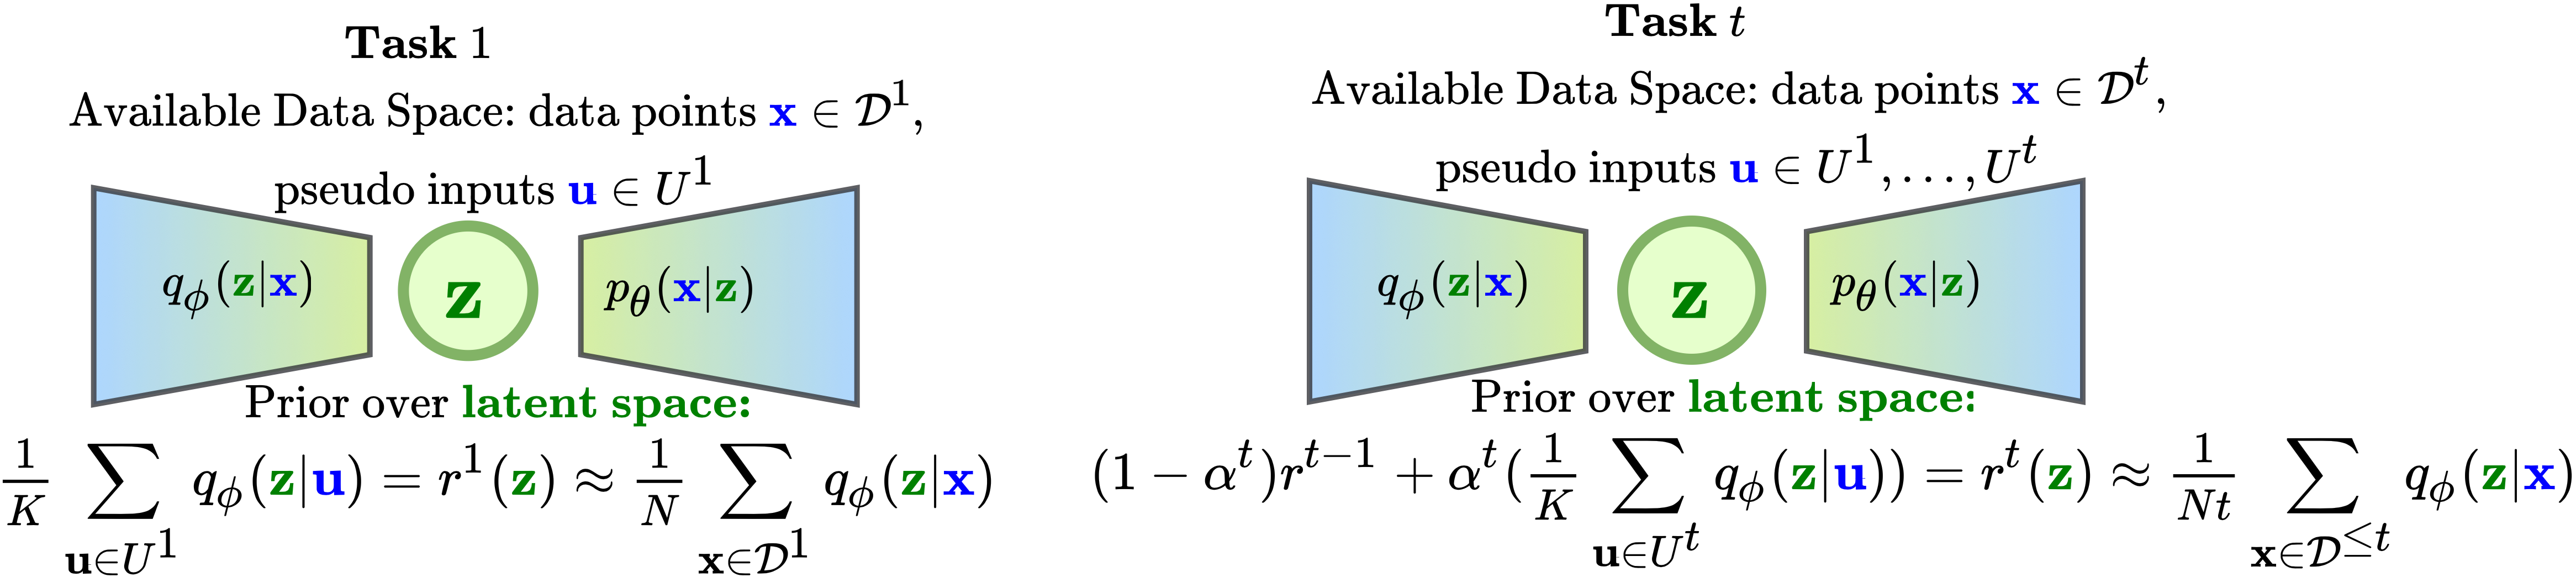
\includegraphics[width=1.0\textwidth]{pics/1_boovae/kek.png}
	\caption{We propose to expand prior distribution in order to match new information from the coming task. We parametrize each component in the prior distribution with encoder, evaluated on the trainable pseudo-inputs. These pseudoinputs store information about the data in the corresponding task.}\label{fig:sheme_inc}
\end{figure}

In this section, we formulate the algorithm for continual learning -- BooVAE (short for Boosting VAE).  
It works as the iterative Minorization-Maximization algorithm. 
In the \textit{minorization step}, we use the obtained optimization problem (Eq.~\ref{eq:final_opt}) to learn a new component of the prior.
These steps are alternated with \textit{ELBO maximization steps} until the desired number of components in prior is reached. From that point further on, only model parameters are updated until convergence. As at maximization step follows the usual routine used in training VAEs, our approach can be easily used on top of any VAE model. The derivations of applications of BooVAE to the VAE with flow-based prior presented in Appendix~\ref{app:flowvae}. These steps are summarized in Algorithm~\ref{alg:boo} and idea of prior learning for continual setting is illustrated in Figure~\ref{fig:sheme_inc}. Now, we are going to consider them in more details.
% \begin{wrapfigure}{R}{0.56\textwidth}
% \vskip -0.2in
% \begin{minipage}[b]{0.56\textwidth}
% \begin{algorithm}[H]
\begin{algorithm}
	\caption{BooVAE algorithm}
	\label{alg:boo}
	\begin{algorithmic}
  \\\hrulefill
  % \baselineskip\hrule{\textwidth}
\State \hskip-3mm  {\bfseries Input:} { Current task $t$ dataset $\mathcal{D}: \,\{x_n\}_{n=1}^N$}
\State \hskip-3mm {\bfseries Input:} { Maximal number of components $K$}
		\State { Prior to approximate:  $\pi^{\leq t}=\alpha r^{t-1} + (1-\alpha)\hat{q}_t $.}
		\State {Initialize prior: $r^{t} = r^{t-1}$}
		\State {$\theta^*, \phi^*  = \argmax_{\theta,\phi} \mathcal{L}(r^{t}, \theta, \phi)$}
		\State $k = 1$
		\While{not converged and $k < K$}
		\State $h^* = \argmin\limits_{h\in\mathcal{R}}\KL{h}{ \frac{ \pi_{\lambda^*}}{r^{t}}}$
		\State $\beta^* = \argmin\limits_{\beta\in(0;1)}\KL{\beta h + (1 - \beta) r^{t}}{\pi^{\leq t}}$
		\State $r^{t} = \beta^* h^* + (1 - \beta^*) r^{t} $
		\State $k = k + 1$
				\State $\theta^*, \phi^*  = \argmax_{\theta,\phi} \mathcal{L}(r^{t}, \theta, \phi) $
		\EndWhile
            \State \hskip-3mm  {\bfseries Output:} $r^{t}$, $\theta^*$, $\phi^*$
	\end{algorithmic}
\end{algorithm}
% \end{minipage}
% \end{wrapfigure}
\paragraph{Prior Update Step} At this step we expand the current approximation of the optimal prior distribution. The subsets $\train^1,\dots, \train^T$ arrive sequentially and may come from different domains. We have access to only one subset of data and current prior at a time but aim to learn the prior distribution $\tfrac{1}{|\train^{\leq T}|}\sum_{\rvx\in\train^{\leq T}}q_{\phi}(\rvz|\rvx)$. At task $t$ we start from the current prior $r^{t}(\rvz):=r^{t-1}(\rvz)$. We expand the current approximation to at most $K$ components. At each step $k$ we add a new component $h$ to the current approximation $r^{t}$ to move it towards an optimal prior $\pi^{\leq t}$. Following \citep{tomczak2018vae}, we select the parametric family $\mathcal{R}$ of the components $h$ as learnable pseudo-inputs $\rvu$ to the encoder: $h(\rvz)=q_{\phi}(\rvz|\rvu)$. This choice connects parameters of the prior with the data-space. We conclude with a two-step procedure for adding a new component:
\begin{enumerate}
	\item Train new component:\newline
	$h^* = \argmin\limits_{h\in\mathcal{R}} \KL{h}{\frac{\pi^{\leq t}}{r^{t}}}$.
	\item Train component weight:\newline
	$\beta^* = \argmin\limits_{\beta\in(0;1)} \KL{\beta h^* + (1 - \beta) r^{t} }{\pi^{\leq t}}$.
	\end{enumerate}
As it was already mentioned, we define the optimal prior to be equal to the aggregate posterior. Therefore, it stores all the information about the training dataset. The optimal prior for tasks $1:t$ can be expressed with the prior from the previous step (e.g. aggregate posterior over tasks $1:t-1$) and the training dataset from the current task only: 
\begin{equation}
\begin{aligned}
& \pi^{\leq t}(\rvz) = \frac{|\train^{\leq t-1}|}{|\train^{\leq t}|} \pi^{\leq t-1}(\rvz) + \frac{|\train^{t}|}{|\train^{\leq t}|}\frac{1}{|\train^{t}|}\sum_{\rvx_n\in\train^{t}}q_{\phi}(\rvz|\rvx_n).
\end{aligned}
\end{equation}
Since we do not have access to the data from previous tasks, we suggest using trained prior $r^{t-1}$ as a proxy for the corresponding part of the mixture. We use a random subset from the current task $\mathcal{M}^t \subset \train^t$ containing $N_{t}$ observations to estimate the aggregated posterior for the current task.
\begin{equation}
\begin{aligned}
& \pi^{\leq t}(\rvz) \approx  \frac{|\train^{\leq t-1}|}{|\train^{\leq t}|} r^{t-1}(\rvz|\{\rvu\}^{\leq t-1}) + \frac{|\train^{t}|}{|\train^{\leq t}|} \frac{1}{N_{t}}\sum_{\rvx \in  \mathcal{M}^t} q_{\phi}(\rvz|\rvx).
\end{aligned}
\end{equation}
This formulation allows an algorithm not to forget information from the previous task, which is stored in the prior distribution and pseudo-inputs $\{\rvu\}^{\leq t-1}$. The prior distribution performs regularization for the VAE model. As the budget of components learning per task is reached, we perform component pruning by weight optimization, see Appendix~\ref{app:stepback}.
\paragraph{ELBO Maximization Step.} At this step parameters of the encoder and decoder $\theta,\phi$ are updated. We add a regularization term to ensure that the model remembers the information which is stored in the pseudo-inputs. Given the fixed mean parameters of the previous task $r^{t-1}$, we keep their components during training the task $t$ as well as distribution of their fixed decoded mean parameters $p^{t-1}(\cdot)$:
\begin{align}\label{eq:reqularizers}
   & R_{enc}(\phi)=\sum_{\rvu\in r^{t-1}}\KLsym{q_{\phi}(\rvz|\rvu)}{r^{t-1}(\rvz|\rvu)}, \\ 
   & R_{dec}(\theta)=\sum_{\rvz \sim r^{t-1}}\KLsym{p_\theta(\rvx|\rvz)}{p^{t-1}(\rvx|\rvz)}.
\end{align}
where $\KLsym{p}{q} = \tfrac12\left(\KL{p}{q} + \KL{q}{p}\right)$. We use symmetric KL-divergence, since we have observed that it helps to avoid encoder and decoder to memorizing delta function centered in the pseudo-input and results in more diverse samples from the previous tasks. 
The final objective for the maximization step over $\phi, \theta$ for the task $t$ is the following:
\begin{equation} \label{eq:obj_with_reg}
    \begin{aligned}
    & \E_{\substack{\rvx\sim\train_t,\\\rvz\sim q(\rvz|\rvx)}}[\log p_{\theta}(\rvx|\rvz) - \KL{q_{\phi}(\rvz|\rvx)}{r^{t}(\rvz)}] - \lambda (R_{enc}(\phi) + R_{dec}(\theta)).
    \end{aligned}
\end{equation}
\section{Related Work}
\paragraph{Boosting density approximation.}
The approximation of the unnormalized distribution with the sequential mixture models has been considered previously in several studies. Several works \citep{miller2017variational,gershman2012nonparametric} perform direct optimization of ELBO with respect to the parameters of the new component. Unfortunately, it leads to an unstable optimization problem. Therefore, other works consider the functional Frank-Wolfe framework, where subproblems are linearized \citep{wang2015functional}. At each step, the KL-divergence functional is linearized at the current approximation point by its convex perturbation, obtaining tractable optimization subproblems over the distribution space for each component. \citet{guo2016boosting} suggested using concave log-det regularization for Gaussian base learners. \citet{egorov2019maxentropy}, \citet{locatello2018boosting} used entropy-based regularization. In our work, we come up with a similar optimization algorithm. We optimize \textit{different objective for different propose}: the weighted sum of exclusive KL to approximate optimal prior for VAE, while the mentioned works approximate inclusive KL, in order to approximate posterior distribution. 
\paragraph{Continual learning for VAE.}
\citet{lesort2019generative} compare EwC, generative replay, and random coresets. We use a single pair of encoder and decoder for all the tasks unless otherwise stated. \citet{nguyen2017variational} propose to use multi-head VAE architecture, where a separate encoder is trained for each task, and an extra head is added to the decoder. We believe that even though this model was shown to produce good results, it has several crucial limitations. Firstly, it makes the scalability of the method very poor, since the number of parameters in the models increases dramatically with the number of tasks. Secondly, task labels must be known both during training and validation to use the suitable "head" for each data point. Finally, it limits the amount of information we can share between tasks, and thus may lead to worse performance for the tasks, which has fewer data available and have a lot of similarities with other tasks. We have observed the latter phenomenon on the CelebA dataset, where all the tasks are supposed to generate images with faces but with different hair colors. Recent work \citep{rao2019continual} uses a learnable mixture as the prior distribution. However, this reached by also expanding the architecture of encoder with multi-heads and using self-replay to overcome forgetting. \citet{achillelife} propose similar ideas of encoder expansion and use also self-replay. However, our goal is to provide orthogonal approach, which avoids self-replay and multi-heads, but can be combined with them.
\section{Experiments}
\label{exper}
We empirically evaluated our algorithm for both disjoint image generation and classification tasks. In the latter case, we suggest using VAE learned in the continual setting for generative replay \citep{shin2017continual}. 

\subsection{Disjoint image generation task}
\paragraph{Setup} We consider an experimental setup, where each task contains objects of 1 class (e.g. one digit for MNIST dataset). The resulting generative model, trained on all the classes one-by-one is supposed to generate images from all the classes. We perform experiments on MNIST \citep{lecun1998mnist} , notMNIST, fashion MNIST \citep{xiao2017fashion}  and CelebA \citep{liu2015faceattributes} datasets. Each of the MNIST datasets has 10 classes with digits, characters, and pieces of clothing correspondingly. For the CelebA dataset we consider 4 tasks based on the attributes: black, blond, brown, and gray hair. For all the datasets, we use VAE \citep{kingma2014autoencoding} model with Gaussian posterior. A complete description of the experimental setup, architectures, and hyperparameters can be found in Appendix~\ref{app:archicture}. 

\paragraph{Compared methods} As a baseline we consider standard VAE model. We expect it to suffer from catastrophic forgetting and use it as a lower bound on the model performance. We refer to this model as \textbf{Standard}.
Our method has some similarities with the regularization-based continual learning algorithms, which add quadratic penalty on the weights. The difference is that we use prior, defined as a mixture of the encoded pseudo-inputs, to avoid catastrophic forgetting both for the encoder and the decoder (Eq.~\ref{eq:reqularizers}). In the experiments we compare with such regularization-based approaches as Elastic Weight Consolidation (\textbf{EWC}) \citep{kirkpatrick2017overcoming} and Variational Continual Learning (\textbf{VCL}) \citep{nguyen2017variational}. 
Our approach uses pseudo-inputs to approximate an optimal prior distribution for each task. This procedure can also be seen as coreset selection \citep{huggins2016coresets, bachem2015coresets}. To validate the quality of the learned coresets, we perform the comparison with \textbf{random coresets}, which was also used in \citep{nguyen2017variational}. We store a random subsample of the training dataset from previous tasks and add them to each batch during training to avoid catastrophic forgetting. 
Moreover, we can learn the prior distribution components in the latent space instead of the data space as we do with the pseudo-inputs. We have conducted experiments, where the prior is trained as a mixture of Gaussian's (with diagonal covariance) in the latent space. We refer to this approach as \textbf{MoG}. Just as we do in BooVAE, in MoG we learn a new mixture of components for each task and use the regularization from Eq.~\ref{eq:reqularizers} to avoid catastrophic forgetting. 
% \begin{figure}[h]
\begin{figure}[t]{}
		     % \vspace*{-\baselineskip}
	\centering
		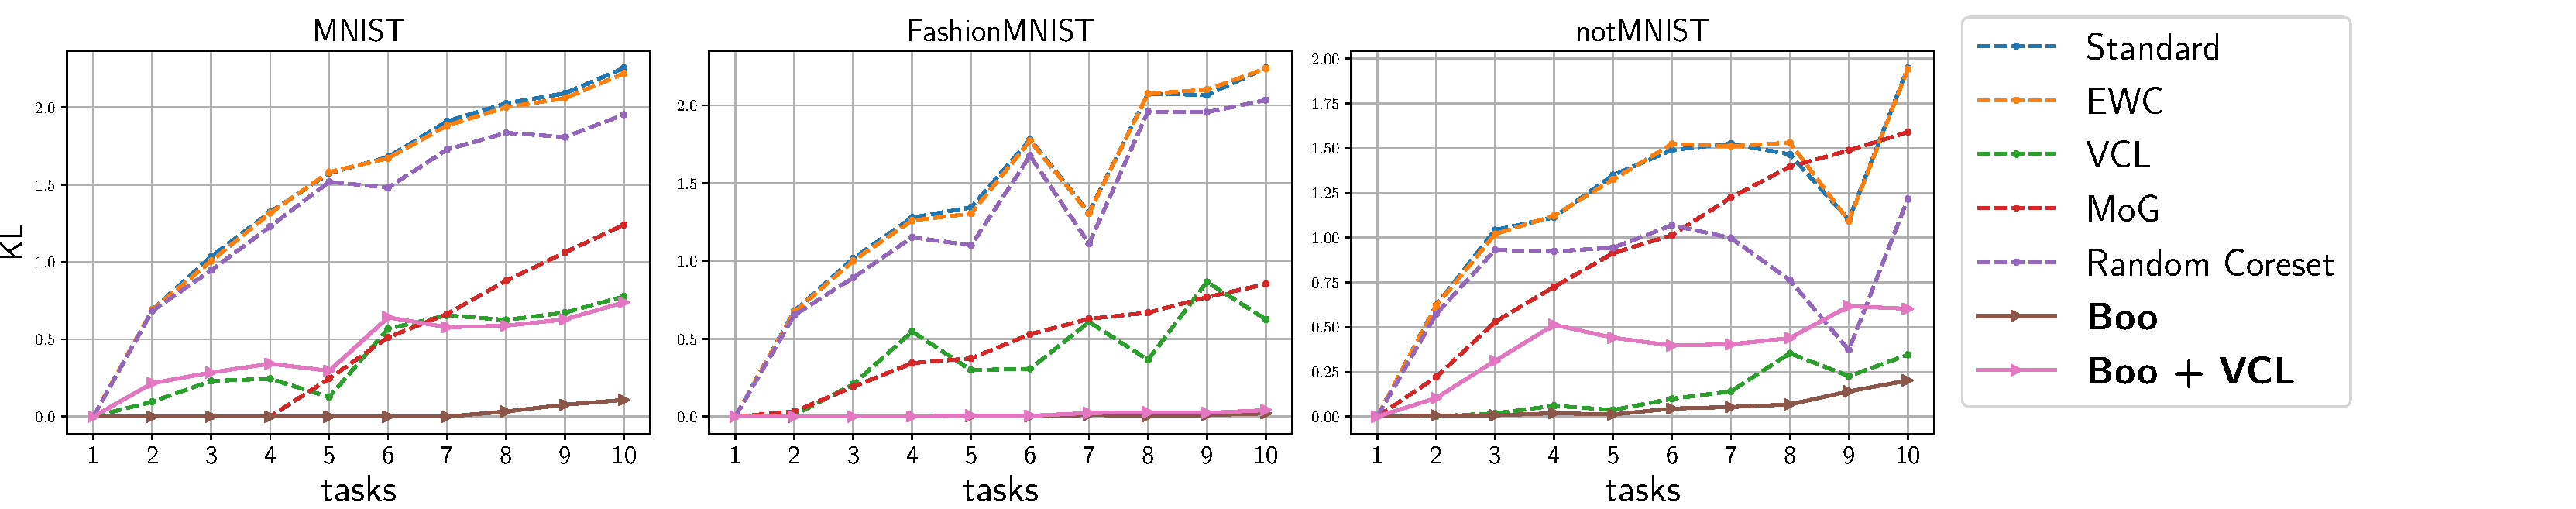
\includegraphics[width=1.1\textwidth]{pics/1_boovae/kl_mnists.pdf}
 \setfloatalignment{t} 
	\caption[][-\baselineskip]{\textbf{Diversity} of generated samples (KL between discrete distribution with the equal probability for each class and empirical distribution of samples from VAE). The lower is the better. We conclude that BooVAE outperforms other approaches.}\label{fig:online:diversity}
	     \vspace*{1.2\baselineskip}
 \end{figure}
 
 \begin{figure}[t]
	\centering
	\vskip \baselineskip
		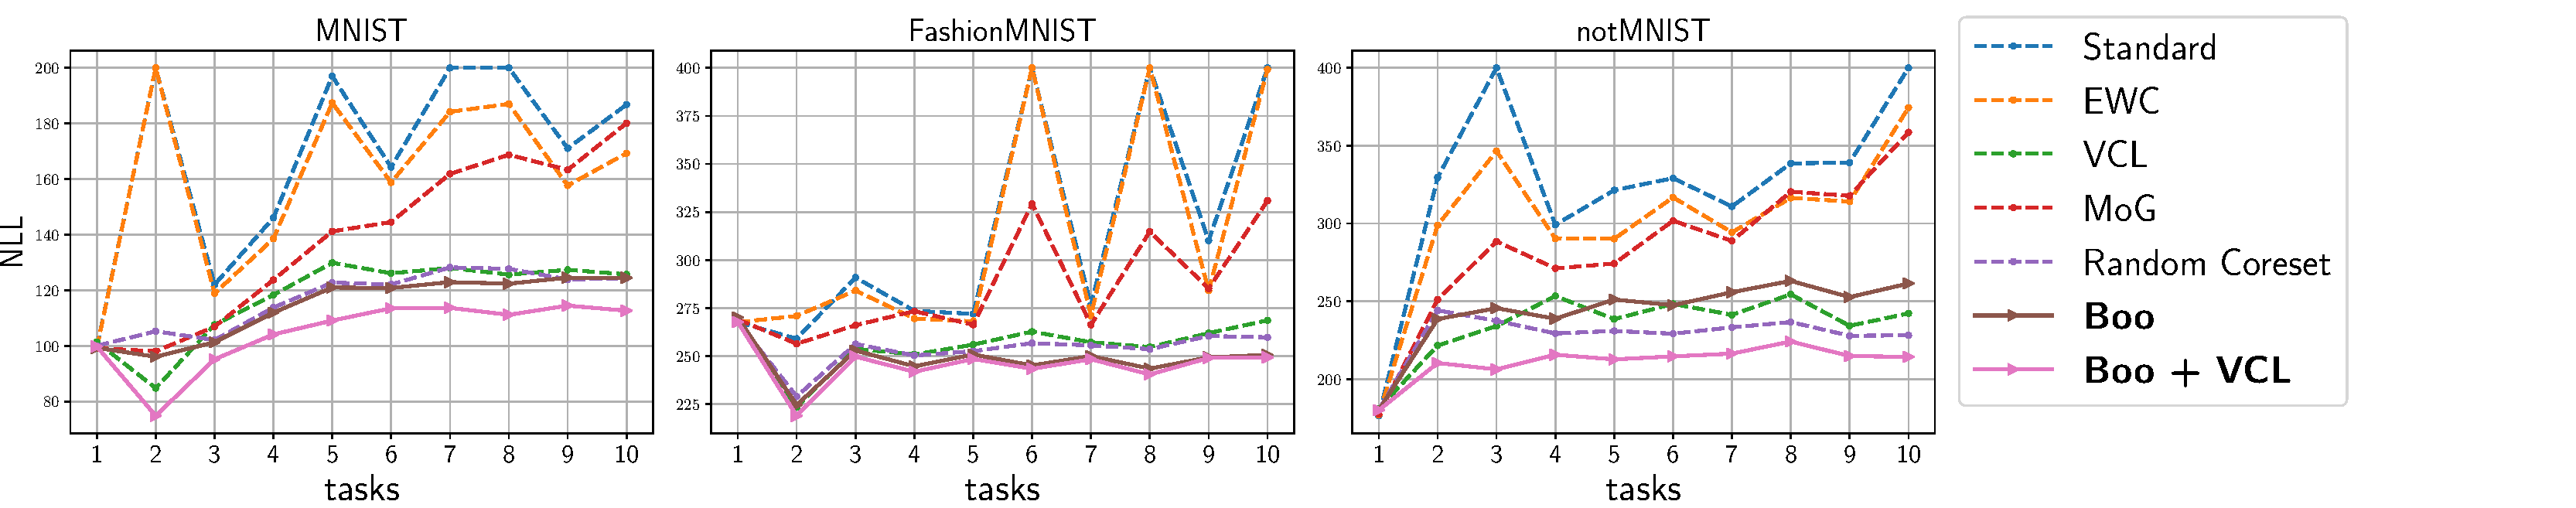
\includegraphics[width=1.1\textwidth]{pics/1_boovae/nll_mnists.pdf}
		 \setfloatalignment{t} 
	\caption[][1.\baselineskip]{\textbf{NLL} on the full test dataset averaged over 5 runs after continually training on 10 tasks. Lower is better. We observe that BooVAE performance is comparable or better than of other methods.}\label{fig:online:NLL} 
	     % \vspace*{-1.5\baselineskip}
\end{figure}

\begin{figure}[t]
	 \setfloatalignment{t} 
		\centering
		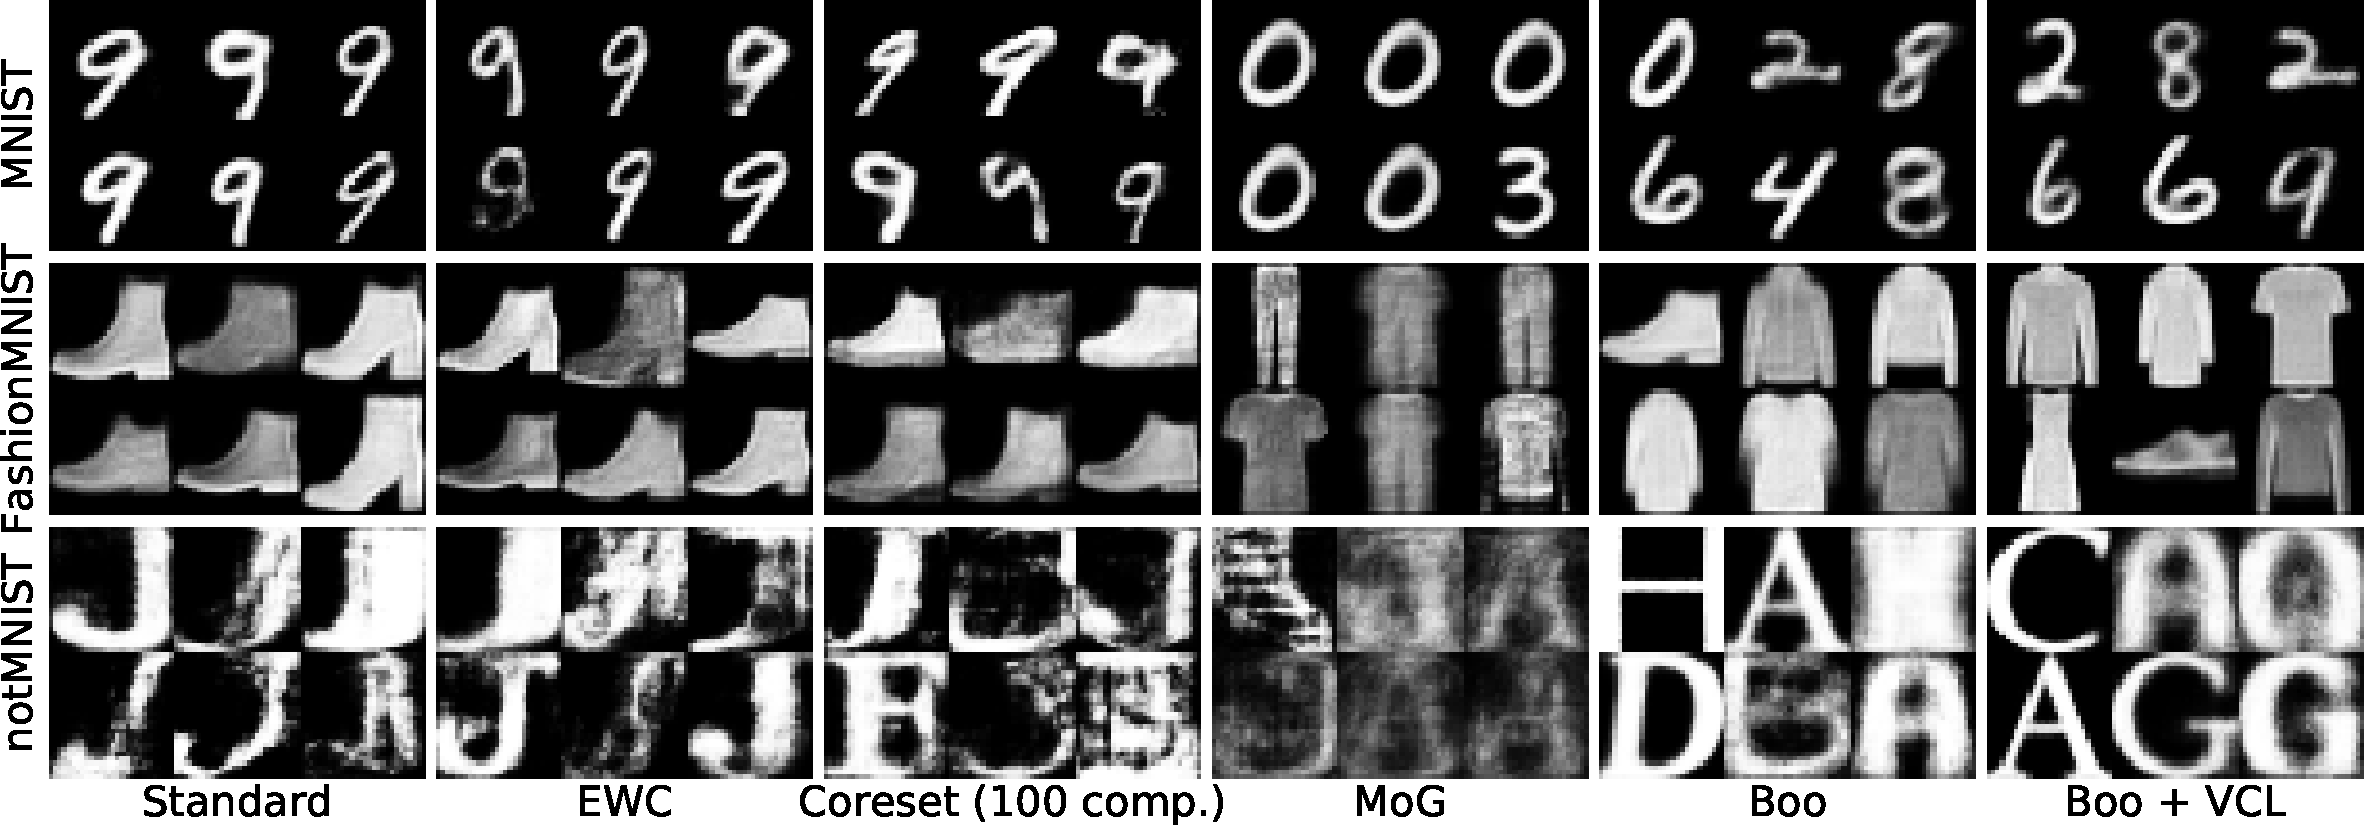
\includegraphics[width=\textwidth]{pics/1_boovae/MNISTSGEN.pdf}
	\caption{Samples from the VAEs after the last task is learned. BooVAE keep sampling different tasks, while other approaches suffer from catastrophic forgetting.}
%	\vskip -3mm
	\label{fig:MNISTSGEN}
\end{figure}

\begin{table}[t]
% \setfloatalignment{t} 
% \captionsetup{width=1.3\textwidth, margin={0pt, -.3\textwidth}}
\caption[][1.1\baselineskip]{FID values for CelebA dataset averaged over 5 runs, the lower is the better. Each row corresponds to the FID for the cumulatively learned tasks of different hair types. BooVAE outperform other approaches, including multihead.}
% \caption{FID values for CelebA dataset averaged over 5 runs, the lower is the better. Each row corresponds to the FID for the cumulatively learned tasks of different hair types. BooVAE outperform other approaches, including multihead.}
\label{tab:celeba_fid}
\begin{center}
\resizebox{1.\textwidth}{!}{
\begin{tabular}{l|ccccccc}
    \toprule
   \multirow{2}{*}{\#T} & \multirow{2}{*}{\small{EWC}} &	\small{Multihead}	& \multirow{2}{*}{\small{VCL}} & \small{Multihead }	& \small{Random }& \small{Random } & \small{Boo}  \\ 
     &  &	\small{+ EWC}	& & \small{ + VCL}	& \small{ Coreset} \small{(40)}& \small{Coreset} \small{(80)}&  \small{(40 comp.)} \\ \midrule
    1 &35.8 \small{(0.8)} &37.7 \small{(1.1)}& 35.8 \small{(0.6)} & 37.93 \small{(1.0)} &36.4 \small{(1.3)}& 38.1 \small{(1.9)}&\textbf{27.5 \small{(0.6)}}       \\
    2 &61.4 \small{(1.7)} &69.2 \small{(1.3)}& 58.7 \small{(0.6)} & 65.54 \small{(0.2)}&59.6 \small{(0.4)}& 59.8 \small{(0.8)}&\textbf{45.7 \small{(2.4)}}             \\
    3 &40.7 \small{(0.6)} &45.2 \small{(0.8)}& 39.3 \small{(0.6)} & 42.18 \small{(0.4)}&39.7 \small{(0.8)}& 41.9 \small{(0.1)}&\textbf{33.4 \small{(1.4)}}             \\
    4 &50.7 \small{(0.6)} &75.7 \small{(0.8)}& 48.7 \small{(0.9)} & 75.16 \small{(2.0)}&48.1 \small{(1.1)}& 47.4 \small{(1.9)}&\textbf{43.1 \small{(0.2)}}             \\
    % \midrule
    \bottomrule 
\end{tabular}
}
    \vspace*{10pt}
\end{center}
\end{table}

\begin{figure}[t]
	     \vspace*{10pt}
		\centering
		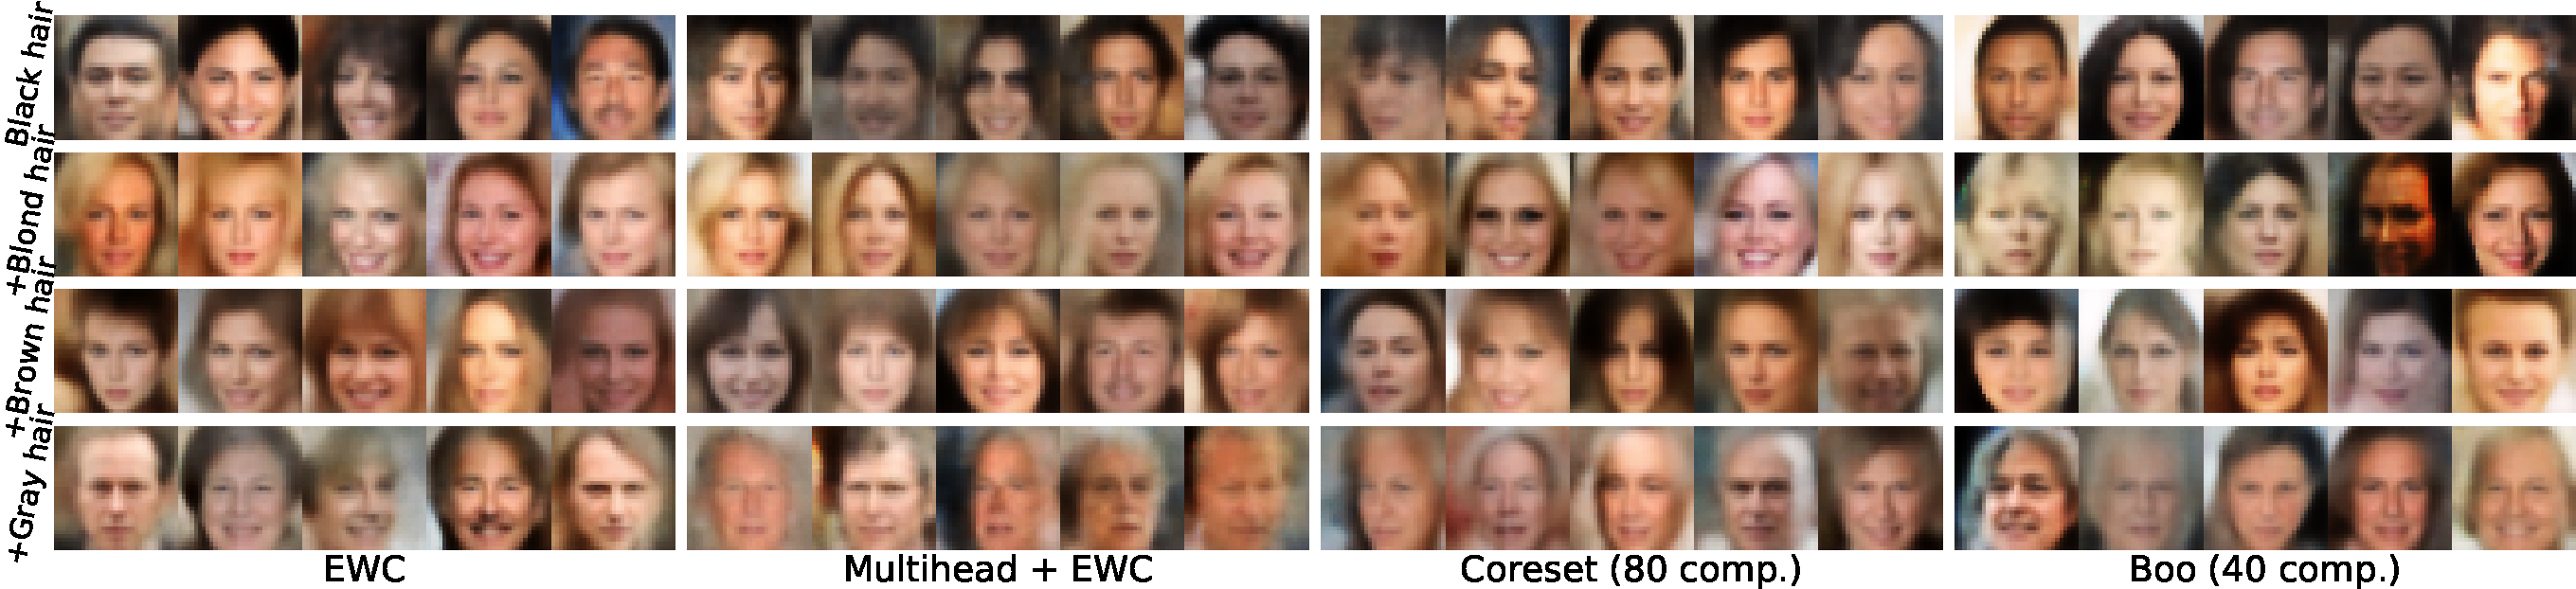
\includegraphics[width=1.\textwidth]{pics/1_boovae/CELEBAGEN.pdf}
	\caption[][\baselineskip]{Samples from VAE trained on CelebA. For each model rows correspond to cumulatively learned tasks of different hair types.}
	\label{fig:CELEBAGEN}
	% \vskip -5pt
\end{figure}
\paragraph{Metrics} To evaluate the performance of the VAE approach on gray scale images, we a standard metric -- negative log-likelihood (\textbf{NLL}) on the test set. NLL is calculated by importance sampling method, using 5000 samples for each test observation: 
\begin{equation*}
\setlength{\abovedisplayskip}{3.5pt}
\setlength{\belowdisplayskip}{3.5pt}
-\log p(x) \approx -\log \tfrac{1}{K} 
\sum_{i = 1}^K \frac{p_\theta(\rvx |\rvz_i) p(\rvz_i)}{q_\phi(\rvz_i | \rvx)},\,\rvz_i \sim q_\phi(\rvz| \rvx).
\end{equation*}
NLL measures the quality of the reconstructions that VAE produces. It is also essential to evaluate the diversity of generated images with respect to all the tasks in the continual setting. In our experiments, each task contains a new class. Thus, we expect our model to generate images from all the classes $t=1,\dots, T$ in the same proportion as they appear in the training dataset. For the dataset with balanced classes, this proportion is equal to $\tfrac{1}{T}$. We assess the diversity using the sum of \textbf{KL-divergences} between $T$ pairs of Bernoulli distributions:
\begin{equation*}
\setlength{\abovedisplayskip}{3.5pt}
\setlength{\belowdisplayskip}{3.5pt}
\sum_{t=1}^{T}\KL{p_t}{\widehat{p}_t},\; p_t \sim \text{Be}\left(\tfrac1T\right),\;  \widehat{p}_t \sim \text{Be}\left(\tfrac{N_t}{\sum_{t=1}^{T}N_t}\right), 
\end{equation*}
where $ \widehat{p}_t$ is an empirical distribution of the generated classes, $N_t$ --- number of generated images from the class $t$. To estimate $N_t$, we train the classification neural network to achieve high accuracy and use it to classify images generated by the model. We use $10^4$ samples in total to calculate the metric.
For the CelebA dataset, we used Frechet Inception Distance (\textbf{FID}) \citep{heusel2017gans} over $10^4$ samples, which is supposed to measure both quality and diversity of generated samples. FID rely heavily on the implementation of Inception network \citep{barratt2018note}; we use PyTorch version of the Inception V3 network \citep{paszke2017automatic}.
\paragraph{Results on MNIST(s)}
In Figures~\ref{fig:online:diversity},\ref{fig:online:NLL} we provide results for three MNIST datasets. 
Both figures depict values averaged over five runs. We report mean values, standard deviations and comparison with the multihead architectures in Appendix~\ref{app:incr}. We evaluate the performance of VAE on the test dataset after each new task is added. The x-axis denotes a total number of tasks seen by the models (and thus, the total number of tasks in the test dataset). The flatter the line is, the less forgetting we observe as a number of tasks increases.  We provide numbers for each task separately in Appendix~\ref{app:pertask}. Notice that BooVAE can be combined with any other weight-regularization method. We have observed that EWC does not improve performance a lot (see Appendix~\ref{app:incr}), therefore we report only results for the combination of BooVAE with VCL, which gives the best performance in terms of NLL.

We observe that, on the basis of the KL metric, pure BooVAE produces the most diverse samples. We plot several samples from the model after training it on ten tasks in Figure~\ref{fig:MNISTSGEN}. For MoG, Random Corsets, and BooVAE, we use the same amount of components equal to 15 for each task. It is worth mentioning that the closer the random corset size is to the size of the training data, the better the performance should be. In the limit case, we can store all the data from the previous tasks, guaranteeing the absence of catastrophic forgetting. Our goal is to reduce the amount of information stored. Thus, we used a pretty small number of components. In Appendix~\ref{app:coreset} we explore how large the random corset should be to get the performance comparable to BooVAE. 

% \begin{wrapfigure}{r}{0.62\textwidth}
%\begin{figure}[t]
%	\centering
%	\begin{tabular}{cc}
%		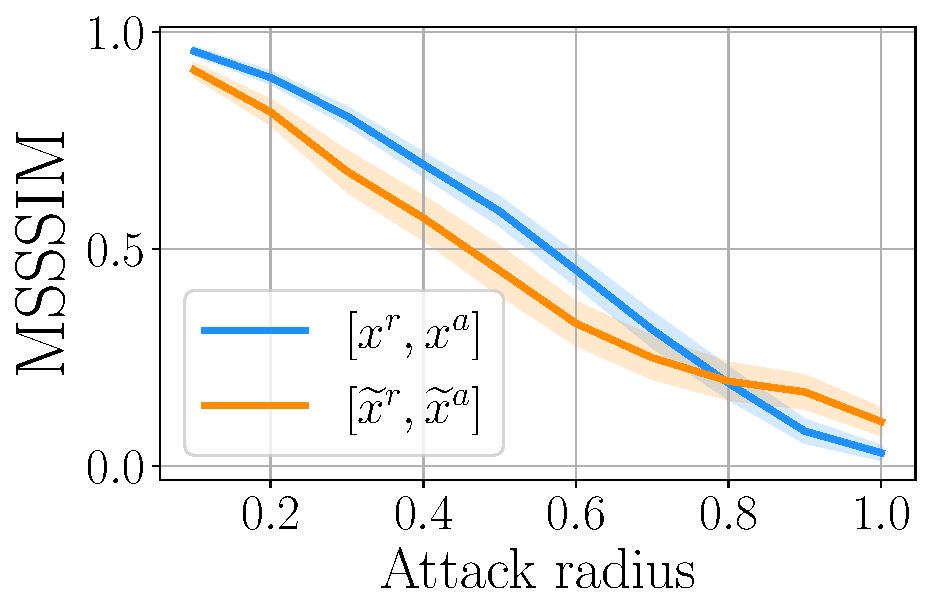
\includegraphics[width=0.4\linewidth]{pics/3_adv_att/attack_mcmc_0_100.pdf} &
%		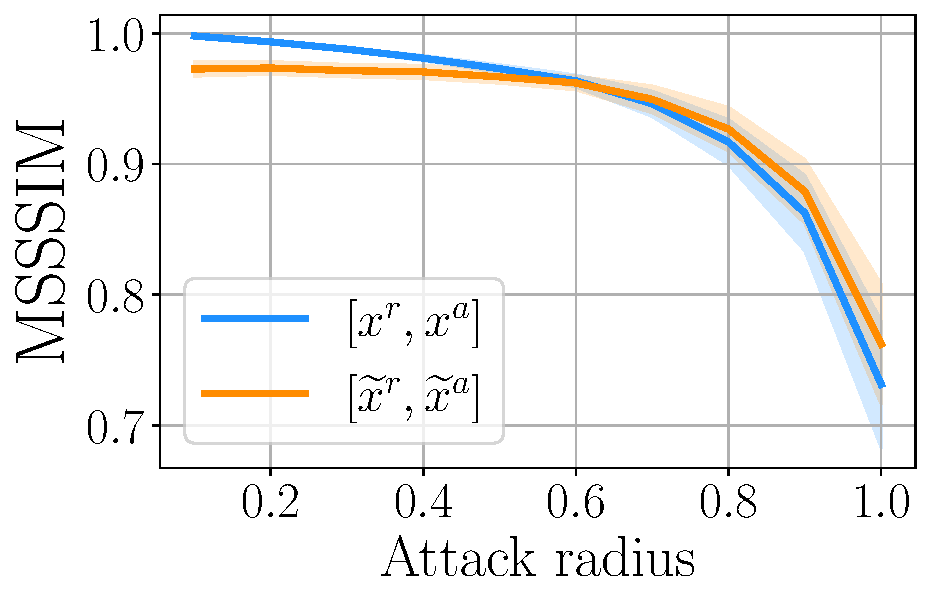
\includegraphics[width=0.4\linewidth]{pics/3_adv_att/attack_mcmc_1_100.pdf} \\
%		\multirow{2}{0.45\linewidth}{\centering \small (a) An attacker does not know the defence strategy}&
%		\multirow{2}{0.45\linewidth}{\centering \small (b) An attacker knows the defence strategy }\\
%		\\
%	\end{tabular}
%	\caption{Robustness to adversarial attack (with HMC defence). We report similarity of the reference and adversarial point (blue) and their reconstructions (orange).}
%	\label{fig:attack_mcmc}
%	\vspace*{\baselineskip}
%\end{figure}

\begin{figure}[t]
	\centering
	\subfloat[MNIST]{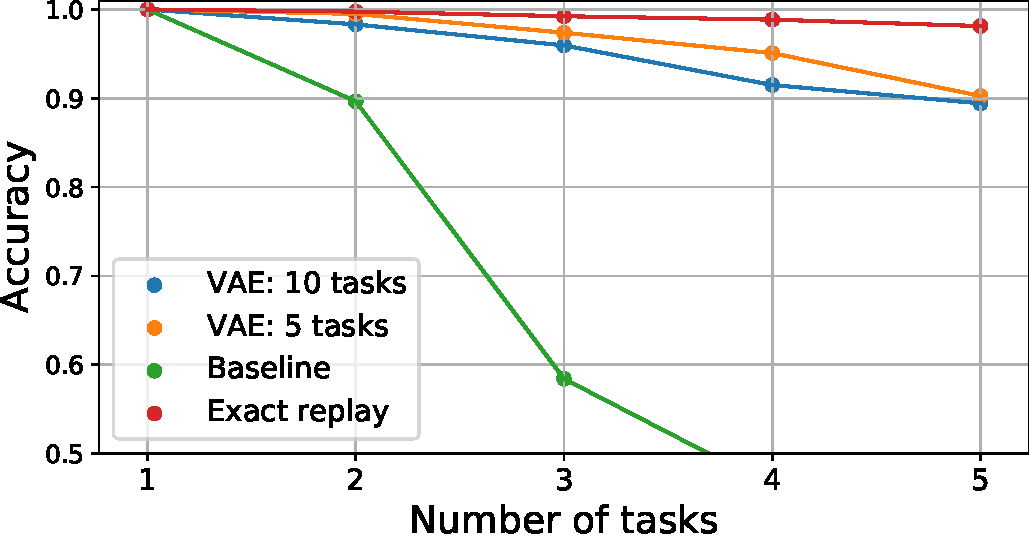
\includegraphics[width=.49\textwidth]{pics/1_boovae/mnist_gen_replay.pdf}}
	\subfloat[Fashion MNIST]{	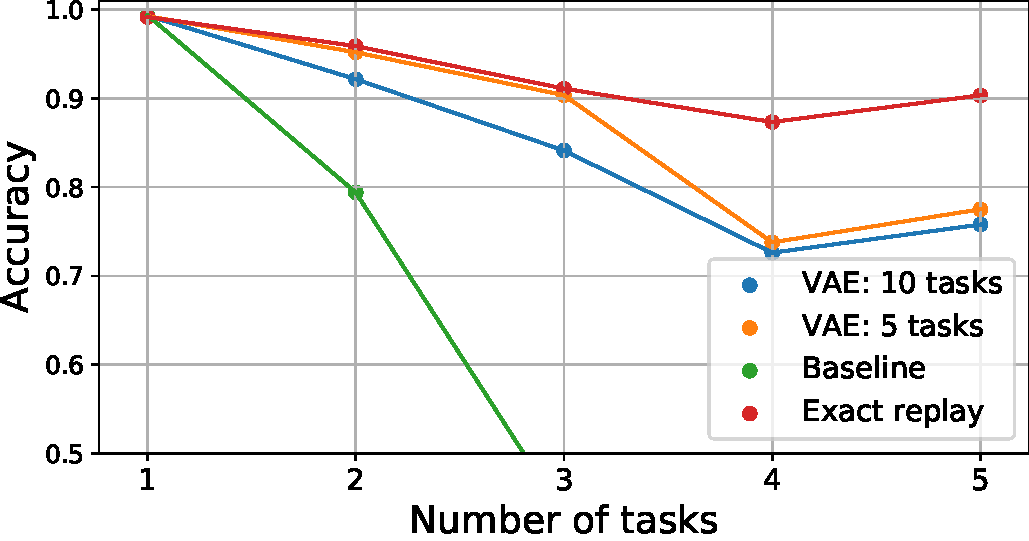
\includegraphics[width=.49\textwidth]{pics/1_boovae/fashion_mnist_gen_replay.pdf}}
	 \setfloatalignment{t} 
		\caption[][\baselineskip]{We consider continual learning experiment for MNIST and Fashion MNIST datasets, where we split the dataset in 5 task, containing pairs of disjoint classes, i.e.  '0/1', '2/3', etc. We train both BooVAE and classification DNN in continual setting, using VAE for generative replay to avoid catastrophic forgetting in classification.}
		\label{fig:gen_relpay}
	\vspace*{\baselineskip}
\end{figure}


%\begin{figure}[!h]
%	\begin{subfigure}[b]{0.5\linewidth}
%	\centering
%		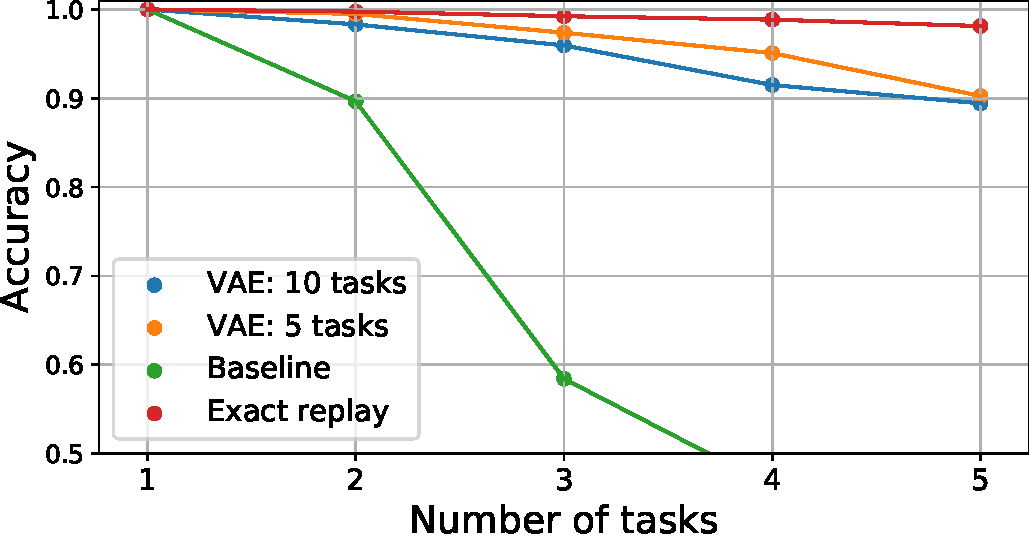
\includegraphics[width=.95\textwidth]{pics/1_boovae/mnist_gen_replay.pdf}
%		\caption{MNIST}
%	\end{subfigure}
%	\begin{subfigure}[b]{0.5\textwidth}
%	\centering
%		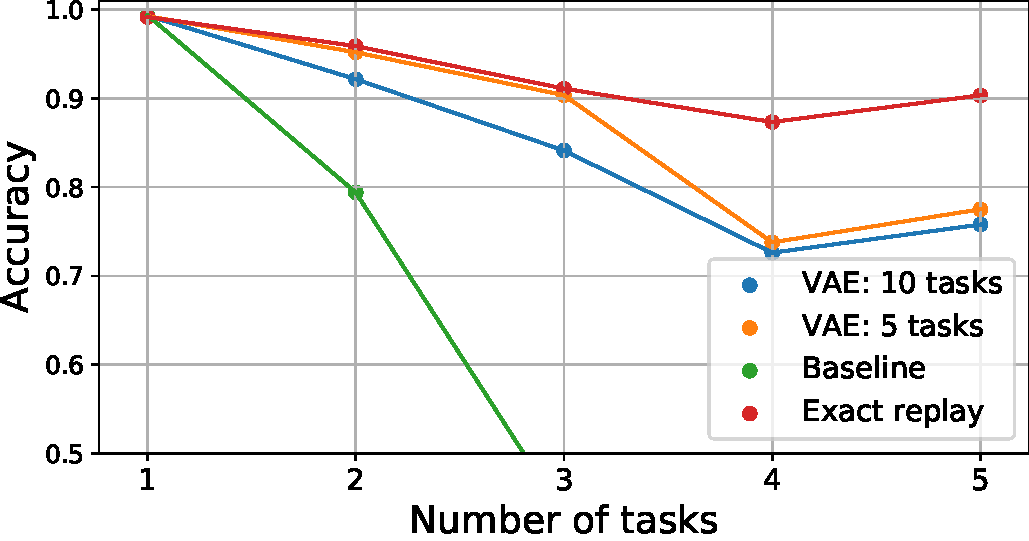
\includegraphics[width=.95\textwidth]{pics/1_boovae/fashion_mnist_gen_replay.pdf}
%		\caption{Fashion MNIST}
%	\end{subfigure}
% \setfloatalignment{t} 
%	\caption{We consider continual learning experiment for MNIST and Fashion MNIST datasets, where we split the dataset in 5 task, containing pairs of disjoint classes, i.e.  '0/1', '2/3', etc. We train both BooVAE and classification DNN in continual setting, using VAE for generative replay to avoid catastrophic forgetting in classification.}
%%	\vskip -3mm
%	\label{fig:gen_relpay}
%\end{figure}
\paragraph{Results on CelebA} We conduct experiments on CelebA dataset for several reasons. Firstly, we want to show that our method works not only on small-scale images, such as MNIST but also on higher-dimensional data. Secondly, since the classes differ only by the hair color in this setting, we may see the advantages of the shared architecture more clearly. In the CelebA dataset there are much fewer faces with grey hair, compared to other colors. Therefore, information from other classes is essential to obtain good results on these images. We compare the FID values as new tasks are added to the models in Table~\ref{tab:celeba_fid}. The BooVAE outperforms other approaches, including model with multihead architecture. Notice that multihead fails on the last task, which has much fewer observations, compared to others. This highlights the benefit of the shared architecture, as  the Multi-heads approach limits the amount of shared information between tasks. Samples from the different VAEs can be found on Figure~\ref{fig:CELEBAGEN}. We provide more samples in Appendix~\ref{app:samples}.
\subsection{Generative Replay for Discriminative Model with continual VAE}
\paragraph{Motivation} Common approach to mitigate catastrophic forgetting in discriminative models is deep generative replay \citep{shin2017continual}. The method is based on the recollection of the past knowledge, such as the data of past classes, by generating it from the trained generative model. However, since continual learning for generative models was limited, it was proposed to re-train the generative model from scratch when a new task arrives. Since we propose the method for the continual learning of the generative model, we can avoid this. We can continually train VAE along with the discriminative model.
\paragraph{Setting} We perform the continual learning experiment using the MNIST and Fashion MNIST datasets. We apply splitMNIST setting when the dataset is split into five binary classification tasks. E.g. the first task containing digits ’0’ and ’1’, the second task --- digits ’2’ and ’3’, and so on. We perform similar splitting into the five tasks for the Fashion MNIST. We train MLP  with two hidden layers, LeakyReLU activations and Dropout layers. For each task, we add a new classification head (one fully connected layer) and train for 200 epochs with batch size 500.  
\paragraph{Results} The mean accuracy across all tasks is reported in Figure~\ref{fig:gen_relpay}. We provide two models for comparison. Exact replay setting reuses all the training data from the previous task, thus, giving an upper bound on the generative replay's performance. In the baseline method, we do not use any information about the previous task. This gives us a lower bound on the performance, i.e. if replay buffer is not used.
We report two versions of the generative replay with VAE. In the first one, we consider each class as a separate task and train VAE in the continual setting (VAE: 10 tasks) and sample images from the last available model. We use prior components to label the image classes. For example, along with the first classification task on MNIST (with digits '0' and '1') we train VAE  firstly on '0's and then on '1's. As a result, we have separate components in the prior distribution for both tasks. Sampling latent vector from these components decoding them gives us the replay buffer for the next classification task. 
In the second setting, we combine classes like in splitMNIST setting, i.e. each task contains two classes (VAE: 5 tasks). In this setting, samples from the prior have to be classified in order to be used in classification model. We follow the approach from \citet{shin2017continual}, using classier from the previous step for this purpose.
Results that we observe are comparable with the MNIST results in \citet{shin2017continual}\footnote{Authors provide only plot (Figure 2 in their paper), therefore we are not able to report exact numbers for comparison}, while our approach avoids full re-training of the generative model.
%\section{Conclusion}
%prior distribution, parametrized by an additive mixture, to memorize information about the learned tasks. The entropy regularization  allows us to reduce the number of components in the approximation of the optimal prior distribution without the loss of performance. In our experiments, we show that method perform on par with state-of-the-art methods. Moreover, we show that it can be successfully combined with other approaches, such as regularization-based ones. 
\section{Conclusion}
\begin{figure}[t]
	\centering
	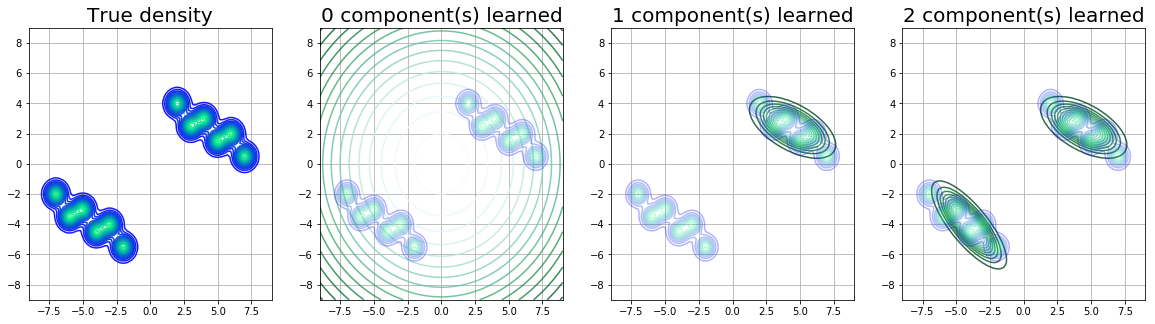
\includegraphics[width=\textwidth]{pics/1_boovae/mpvi_toy.png}
	 \setfloatalignment{t} 
		\caption{The mixture of 12 Gaussian is approximated by 2-component Gaussian mixture with Eq.~\protect\ref{eq:projection}. This toy experiment illustrates the intuition of our approach, where we hope to efficiently approximate prior $\pi^{*}(\rvz)=\E_{p_{e}(\rvx)}q_{\phi}(\rvz|\rvx)$ given only empirical version of the target density $\frac{1}{N}\sum_{n=1}^{N}q_{\phi}(\rvz|\rvx_n)$.}
	\label{fig:mpvi_toy}
%	\vskip -0.1in
\end{figure}
We propose a novel algorithm for continual learning of VAEs with the static architecture by incorporating the data-driven information about new task into the prior over the latent space.
We leverage the specific structure of the VAE model and match new data innovation with the additive aggregated posterior expansion. The boosting-like approach allows us to reduce the number of components in the approximation of the optimal prior distribution without the loss of performance. We empirically validate performance of our algorithm and compare with other approaches. That being said, the proposed algorithm is orthogonal to them and could be easily combined. We would like to finalize with additional comments on performance evaluation and approach intuition.

\paragraph{Model perfomance} In the continual learning setting it is important to evaluate the evolution of the metrics for each task while the new task arrives. Hence in Appendix~\ref{app:incr} - \ref{app:samples} we provide more detailed overview of models performance and report NLL and diversity metric after each additional task is trained. We discuss how performance changes on the whole test dataset as we keep training in continual learning setting. Moreover, we report and discuss these metrics for each task separately in Appendix~\ref{app:pertask}. Finally, we visually study the samples from the model on each step in Appendix~\ref{app:samples}. 
\paragraph{Approach intuition} We provide a toy example visualization in Figure~\ref{fig:2dkek},\ref{fig:mpvi_toy} to illustrate equations in Section~\ref{sec:boovae}.
%\begin{figure}[t!]
%	\begin{subfigure}[b]{0.5\textwidth}
%	\centering
%		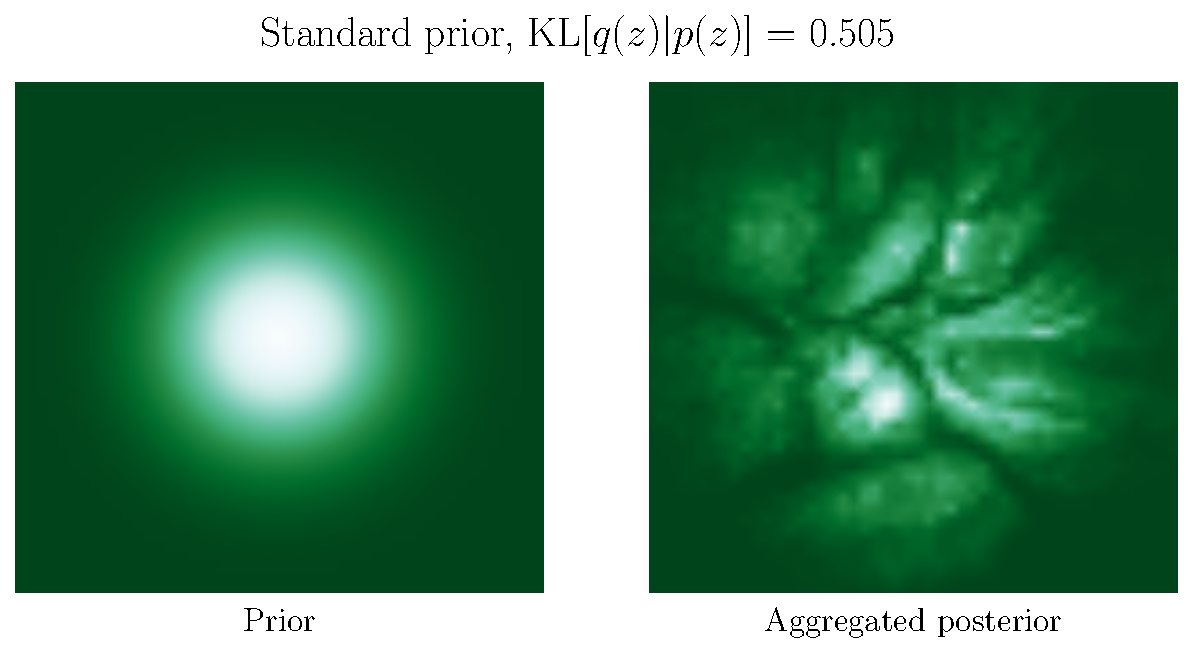
\includegraphics[width=0.99\textwidth]{pics/1_boovae/2dKL_std.pdf}
%	\end{subfigure} 
%	\begin{subfigure}[b]{0.5\textwidth}
%	\centering
%		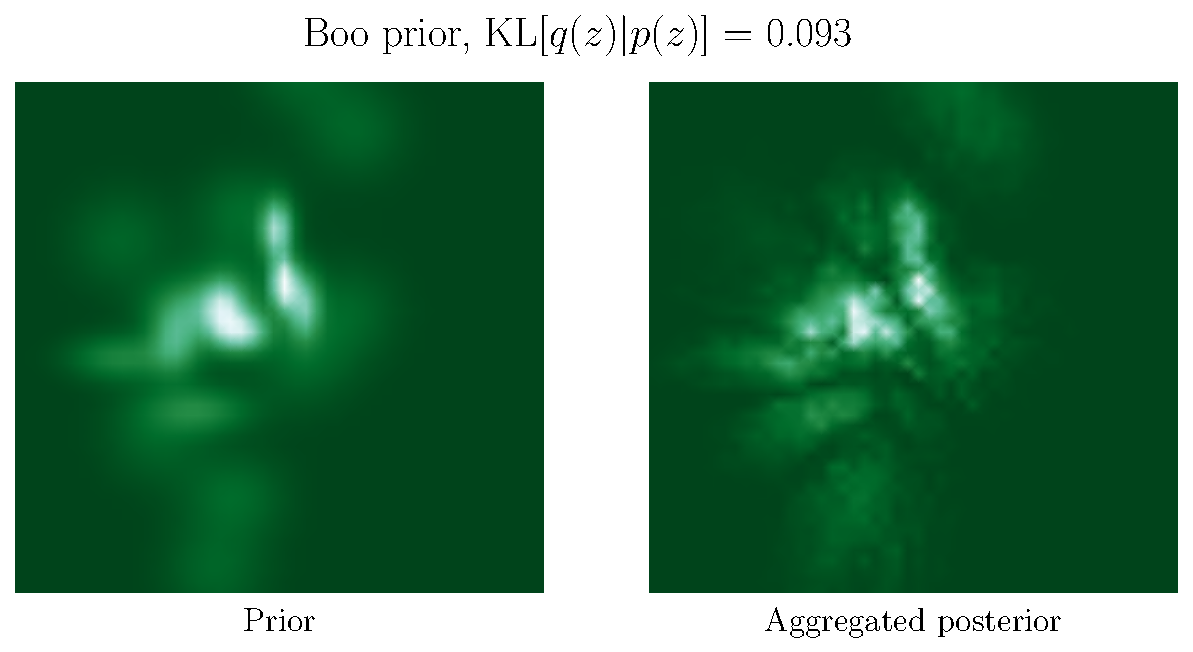
\includegraphics[width=0.95\textwidth]{pics/1_boovae/2dKL_boo20.pdf}
%	\end{subfigure}
%	\caption{Visualization of the prior density and aggregate posterior for the VAE with 2-d latent space. In left we present results for the VAE with $\mathcal{N}(\rvz|\vec{0}, I)$ prior and in the right with the proposed Boo prior. By visual inspection and KL-divergence comparison we conclude that the proposed prior matches the aggregated posterior better that a standard normal prior.}\label{fig:2dkek}
%	\vskip -0.2in
%\end{figure}
\begin{figure}[t!]
	\centering
	\subfloat{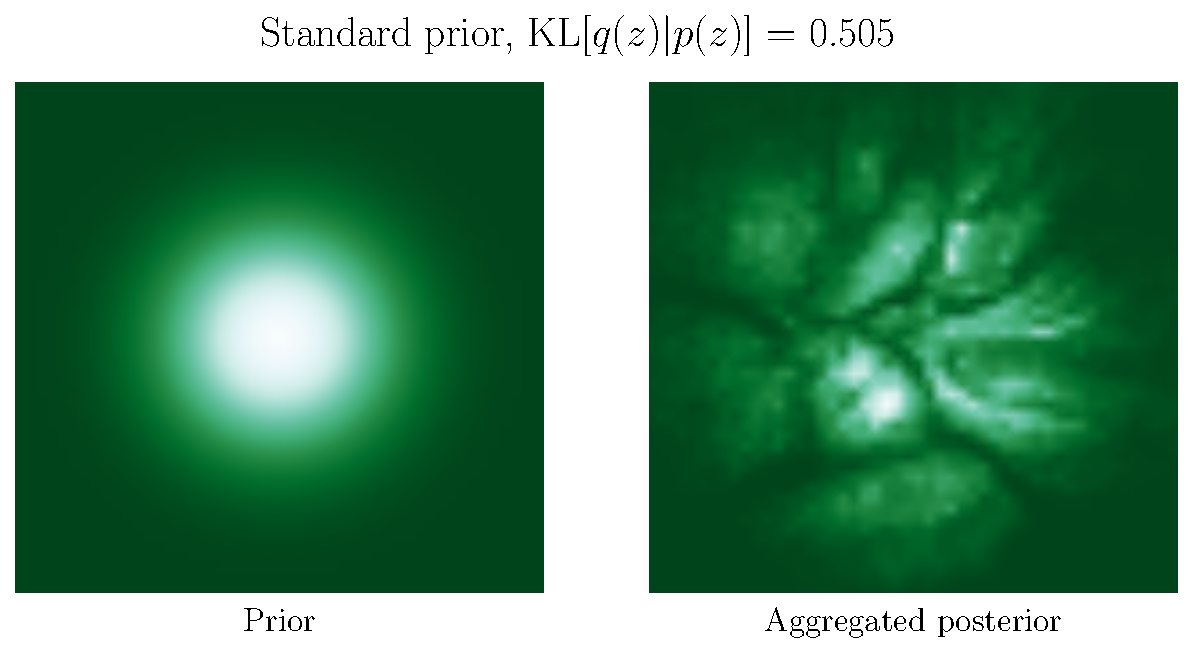
\includegraphics[width=0.5\textwidth]{pics/1_boovae/2dKL_std.pdf}} \hfill
	\subfloat{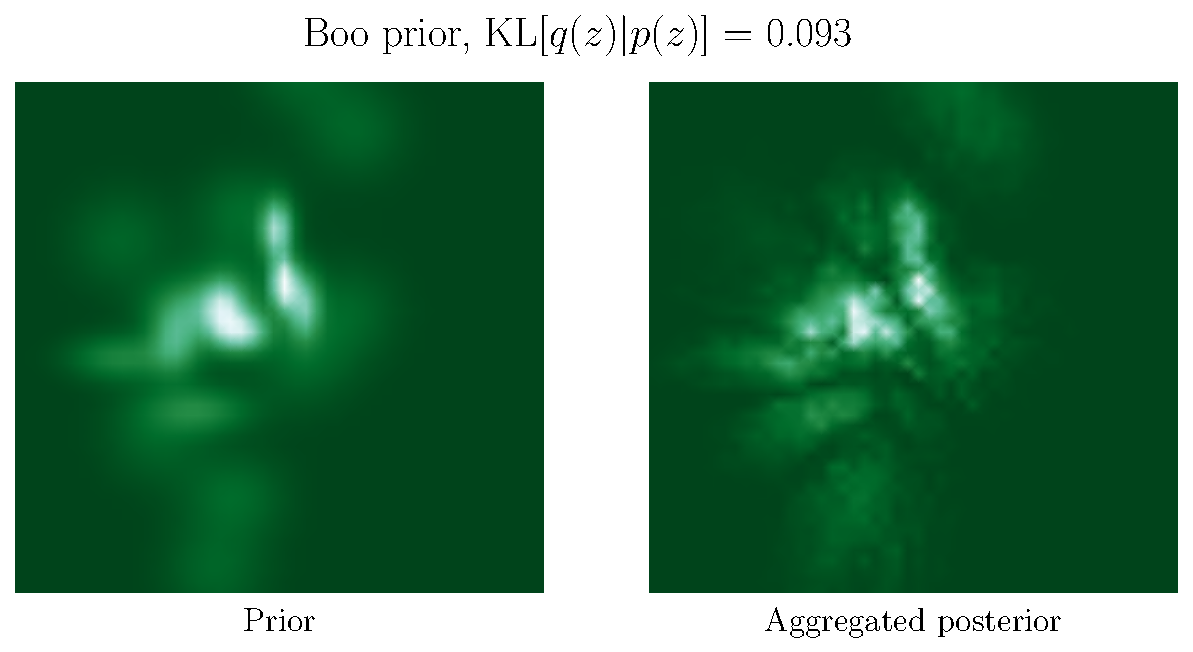
\includegraphics[width=0.5\textwidth]{pics/1_boovae/2dKL_boo20.pdf}}
	\setfloatalignment{t} 
		\caption[][\baselineskip]{Visualization of the prior density and aggregate posterior for the VAE with 2-d latent space. In left we present results for the VAE with $\mathcal{N}(\rvz|\vec{0}, I)$ prior and in the right with the proposed Boo prior. By visual inspection and KL-divergence comparison we conclude that the proposed prior matches the aggregated posterior better that a standard normal prior.}\label{fig:2dkek}
	\vspace*{\baselineskip}
\end{figure}
% \section*{Acknowledgments}
% Authors are thankful to Jakub Tomczak for feedback and inspiring words, to Kirill Neklyudov and Dmitry Molchanov for important discussions during 2019 and to the reviewers who provided detailed feedback. 
% The work of Evgeny Burnaev was supported by Ministry of Science and Higher Education grant No. 075-10-2021-068.




% Я был лишь тем, что ты
% там, внизу, различала:
% смутный облик сначала,
% много позже — черты.
    % Иосиф Бродский


% \usepackage{booktabs, tabularx}       % professional-quality tables
% \usepackage{graphicx}
% \usepackage{multicol, multirow}
% \usepackage{amssymb}
% \usepackage{algorithm}
% \usepackage{algpseudocode}
% \usepackage{adjustbox}
% \usepackage{array}
% \usepackage{wrapfig}
% \usepackage{subfig}
% \usepackage{pifont}

% \usepackage{enumitem}
% \usepackage{capt-of}
% \usepackage{varwidth}
% \newsavebox\tmpbox

% \newcommand{\STAB}[1]{\begin{tabular}{@{}c@{}}#1\end{tabular}}

% \usepackage{hyperref}
% \usepackage{url}

\chapter{Hierarchical VAE with a Diffusion-based VampPrior}\label{chap:dvp}
% Я был лишь тем, что ты
% там, внизу, различала:
% смутный облик сначала,
% много позже — черты.
    % Иосиф Бродский
\begin{quote}
\normalsize\itshape
\begin{flushright}
% \foreignlanguage{russian}{Я был лишь тем, что ты}\\
% \foreignlanguage{russian}{там, внизу, различала:}  \\
\foreignlanguage{russian}{...смутный облик сначала,}\\
\foreignlanguage{russian}{много позже — черты.}  \\
\foreignlanguage{russian}{Иосиф Бродский} \\ \vskip 20pt
 % And the questions...  The questions lack answers, still missing:\\
 % They'll come and they'll burn, fade like measles, unkind.\\
 % Sasha Chorny
\end{flushright}
\end{quote}


\begin{verse}
\textit{
\hfill This chapter is based on the TMLR 2024 paper \citep{kuzina2024hierarchical}.
} 
\end{verse}

\paragraph{Abstract}
Deep hierarchical variational autoencoders (VAEs) are powerful latent variable generative models. 
In this paper, we introduce Hierarchical VAE with Diffusion-based Variational Mixture of the Posterior Prior (VampPrior).
We apply amortization to scale the VampPrior to models with many stochastic layers. 
The proposed approach allows us to  achieve better performance compared to the original VampPrior work and other deep hierarchical VAEs, while using fewer parameters.
We empirically validate our method on standard benchmark datasets (MNIST, OMNIGLOT, CIFAR10) and demonstrate improved training stability and latent space utilization.
\newpage

%%%%%%%%%%%%%%%%%%%%%%%%%%%%%%%%%%%%%%%%%%
% -------------------------------
% ==== SECTION: Introduction ====
%--------------------------------
\section{Introduction}

Latent variable models (LVMs) parameterized with neural networks constitute a large group in deep generative modeling \citep{tomczak2022deep}. One class of LVMs, Variational Autoencoders (VAEs) \citep{kingma2014autoencoding, rezende2014stochastic}, utilize amortized variational inference to efficiently learn distributions over various data modalities, e.g., images \citep{kingma2014autoencoding}, audio \citep{van2017neural}, or molecules \citep{gomez2018automatic}. 
% One of the problems that hinders the performance of VAEs is the \textit{posterior collapse}  \citep{wang2021posterior} when the variational posterior (partially) matches the prior distribution (e.g., the standard Gaussian distribution). 
The expressive power of VAEs can be improved by introducing a hierarchy of latent variables. 
The resulting hierarchical VAEs, such as ResNET VAEs \citep{kingma2016improved}, BIVA \citep{maaloe2019biva}, very deep VAE (VDVAE) \citep{Child2020-ze}, or NVAE \citep{vahdat2020nvae} achieve state-of-the-art performance on images in terms of the negative log-likelihood (NLL). However, hierarchical VAEs are known to have training instabilities \citep{vahdat2020nvae}. To mitigate these issues, various \textit{tricks} were proposed, such as gradient skipping \citep{Child2020-ze}, spectral normalization \citep{vahdat2020nvae}, or softmax parameterization of variances \citep{hazami2022efficientvdvae}. In this work, we propose a different approach that focuses on two aspects of hierarchical VAEs: (i) the structure of latent variables, and (ii) the form of the prior for the given structure. We introduce several changes to the architecture of parameterizations (i.e. neural networks) and the model itself. As a result, we can train a powerful hierarchical VAE with gradient-based methods and ELBO as the objective without any \textit{hacks}.

In the VAE literature, it is a well known fact that the choice of the prior plays an important role in the resulting VAE performance \citep{chen2016variational, tomczak2022deep}. For example, VampPrior \citep{tomczak2018vae}, a form of the prior approximating the aggregated posterior, has been shown to consistently outperform VAEs with a standard prior and a mixture prior. 
In this work, we extend the VampPrior to deep hierarchical VAEs in an efficient manner. 
We propose utilizing a non-trainable linear transformation like Discrete Cosine Transform (DCT) to obtain pseudoinputs. Together with our architecture improvements, we can achieve state-of-the-art performance, high utilization of the latent space, and stable training of deep hierarchical VAEs.

The contributions of the paper are the following:
\begin{itemize} %[itemindent=0pt,leftmargin=15pt]
    \item We propose a new VampPrior-like approximation of the optimal prior (i.e., the aggregated posterior) which can efficiently scale to deep hierarchical VAEs.
    \item We propose a latent aggregation component that consistently improves the utilization of the latent space of the VAE.
    \item Our proposed hierarchical VAE with the new class of priors outperforms other hierarchical VAE models (without additional data augmentations).
\end{itemize}



%--------------------------------
% ==== SECTION: Background ====
%--------------------------------
\section{Background}

% ==== SubSECTION ====
\subsection{Hierarchical Variational Autoencoders} \label{sec:5_dvp_vae}

Let us consider random variables $\rvx \in \mathcal{X}^{D}$ (e.g. $\mathcal{X} = \mathbb{R}$). We observe $N$ $\rvx$'s sampled from the empirical distribution $r(\rvx)$. We assume that each $\rvx$ has $L$ corresponding latent variables $\rvz_{1:L} = (\rvz_1, \dots, \rvz_L)$, where $\rvz_l \in \mathbb{R}^{M_{l}}$ and $M_l$ is the dimensionality of each variable. We aim to find a latent variable generative model with unknown parameters $\theta$, $p_{\theta}(\rvx, \rvz_{1:L}) = \Dec{\rvx}{\rvz_{1:L}} p_{\theta}(\rvz_{1:L})$. 

In general, optimizing latent-variable models with nonlinear stochastic dependencies is non-trivial. A possible solution is approximate inference, e.g., in the form of variational inference \citep{jordan1999introduction} with a family of variational posteriors over latent variables $\{\Enc{\rvz_{1:L}}{\rvx}\}_{\phi}$. This idea is exploited in Variational Auto-Encoders (VAEs) \citep{kingma2014autoencoding, rezende2014stochastic}, in which variational posteriors are referred to as encoders. As a result, we optimize a tractable objective function called the \textit{Evidence Lower BOund} (ELBO) over the parameters of the variational posterior, $\phi$, and the generative part, $\theta$, that is:
\begin{equation}\label{eq:vae_elbo}
\begin{aligned}
\E_{r(\rvx)} &\left[\ln p_{\theta}(\rvx)\right]  \\
&\geq \E_{r(\rvx)} \biggl[ \E_{\Enc{\rvz_{1:L}}{\rvx}}\ln \Dec{\rvx}{\rvz_{1:L}} - \KL{\Enc{\rvz_{1:L}}{\rvx}}{p_{\theta}(\rvz_{1:L})} \biggr] ,
\end{aligned}
\end{equation}

where $r(\rvx)$ is the empirical data distribution. Further, to avoid clutter, we will use $\E_{\rvx}\left[\cdot\right]$ instead of $\E_{r(\rvx)}\left[\cdot\right]$, meaning that the expectation is taken with respect to the empirical distribution. 
% In addition, we use $r^{\text{test}}(\rvx)$ for the hold-out data, where relevant.

% ==== SubSECTION ====
\subsection{VampPrior}
The latent variable prior (or marginal) plays a crucial role in the VAE performance, which motivates the usage of data-dependent priors. 
Note that the KL-divergence term in the ELBO (see Eq.~\ref{eq:vae_elbo}) can be expressed as follows \citep{hoffman2016elbo}:
\begin{equation}
    \mathbb{E}_{\rvx} \KL{q_{\phi}(\rvz|\rvx)}{p(\rvz)} = \KL{q_{\phi}(\rvz)}{ p(\rvz)} + \mathbb{E}_{\rvx} \biggl[ \KL{q_{\phi}(\rvz|\rvx)}{q(\rvz)} \biggr] .
\end{equation}

Therefore, the optimal prior that maximizes the ELBO has the following form:
\begin{equation}\label{eq:optimal_prior}
    p^*(\rvz) = \mathbb{E}_{\rvx} \left[ q_{\phi}(\rvz|\rvx) \right].
\end{equation}

The main problem with the optimal prior in Eq.~\ref{eq:optimal_prior} is the summation over all $N$ training datapoints. Since $N$ could be very large (e.g., tens or hundreds of thousands), using such a prior is infeasible due to potentially very high memory demands. As an alternative approach, \citet{tomczak2018vae} proposed VampPrior, a new class of priors that approximate the optimal prior in the following manner:
\begin{equation} \label{eq:vamp_prior_approx}
    p^*(\rvz) = \mathbb{E}_{\rvx} q_{\phi}(\rvz|\rvx) \approx \mathbb{E}_{r(\rvu)} q_{\phi}(\rvz|\rvu),
\end{equation}
where $\rvu$ is a \textit{pseudoinput}, i.e., a variable mimicking real data, $r(\rvu) =\frac{1}{K}\sum_k \delta(\rvu - \rvu_k)$ is the distribution of $\rvu$ in the form of the mixture of Dirac's deltas, and $\{u_k\}_{k=1}^K$ are learnable parameters (we will refer to them as pseudoinputs as well). $K$ is a hyperparameter and is assumed to be smaller than the size of the training dataset, $K < N$. Pseudoinputs are randomly initialized before training and are learned along with model parameters by optimizing the ELBO objective using a gradient-based method. 
% :  parameter and has less components than number of  points in the dataset.

In follow-up work, \citet{egorov2021boovae} suggested using a separate objective for pseudoinputs (a greedy boosting approach) and demonstrated the superior performance of such formulation in the continual learning setting. Here, we will present a different approximation to the optimal prior instead.

% ==== SubSECTION ====
\subsection{Ladder VAEs (a.k.a. Top-down VAEs)} \label{sec:hierarchical_vae}
% \ak{Here talk more about orignal Ladder VAE and how VDVAE and NVAE differ from those}
We refer to models with many stochastic layers $L$ as deep hierarchical VAEs. They can differ in the way the prior and variational posterior distributions are factorized and parameterized. Here, we follow the factorization proposed in Ladder VAE \citep{sonderby2016ladder} that considers the prior distribution over the latent variables factorized in an autoregressive manner:
\begin{equation}
 p_{\theta}(\rvz_1, \ldots, \rvz_L) = p_{\theta}(\rvz_L)\prod_{l=1}^{L-1}\Dec{\rvz_{l}}{\rvz_{l+1:L}} .
\end{equation}
Next, using the top-down inference model results in the following variational posterior~\citep{sonderby2016ladder}: 
\begin{equation}
\Enc{\rvz_1, \ldots, \rvz_L}{\rvx} = \Enc{\rvz_L}{\rvx}\prod_{l=1}^{L-1}\Enc{\rvz_l}{\rvz_{l+1:L}, \rvx}.    
\end{equation}
This factorization has been previously used by successful deep hierarchical VAEs, among others, 
% BIVA~\citep{maaloe2019biva}, % AK: bive uses different factorization (bi-directional instead of the ladder)
NVAE~\citep{vahdat2020nvae} and Very Deep VAE (VDVAE)~\citep{Child2020-ze}. It was shown empirically that such a formulation allows one to achieve state-of-the-art performance of the hierarchical VAEs on several image datasets. 
% \input{text/1_2_latent_space_properties_background}

%-------------------------------
% ====== SECTION: Method ======
%-------------------------------

%---------------
%----SECTION----
%---------------
% \newpage
\section{Our model: Diffusion-based VampPrior VAE} \label{sec:proposed_approach}
In this work, we introduce the Diffusion-based VampPrior VAE (DVP-VAE). It is a deep hierarchical VAE model that approximates the optimal prior distribution at all levels of the hierarchical VAE in an efficient way.

\subsection{VampPrior for hierarchical VAE}
Directly using the VampPrior approximation (see Eq.~\ref{eq:vamp_prior_approx}) for deep hierarchical VAE can be very computationally expensive since it requires evaluating the variational posterior of all latent variables for $K$ pseudoinputs at each training iteration. Thus, \citet{tomczak2018vae} proposed a modification in which only the top latent variable uses VampPrior, namely:
\begin{equation}\label{eq:hierarchical_vamp}
\begin{aligned}
p^*(\rvz_{1:L}) &= \mathbb{E}_{\rvx} q_{\phi, \theta}(\rvz_{1:L}|\rvx) \\
&\approx \mathbb{E}_{\rvx} q_{\phi, \theta}(\rvz_{L}|\rvx) p_{\theta}(\rvz_{1:L-1})  \\
&\approx \mathbb{E}_{r(\rvu)} q_{\phi, \theta}(\rvz_{L}|\rvu) p_{\theta}(\rvz_{1:L-1}),
\end{aligned}
\end{equation}
where $r(\rvu) = \frac1K \sum_k \delta(\rvu - \rvu_k)$ with learnable pseudoinputs $\{u_k\}_{k=1}^K$.
In this approach, there are a few problems: (i) how to pick the \textit{best} number of pseudoinputs $K$, (ii) how to train pseudoinputs, and (iii) how to train the VampPrior in a scalable fashion. The last issue results from the first two problems and the fact that the dimensionality of pseudoinputs is the same as the original data, i.e., $\mathrm{dim}(\rvu) = \mathrm{dim}(\rvx)$.

Here, we propose a different prior parameterization to overcome all these three problems. Our approach consists of three steps in which we approximate the VampPrior at all levels of the deep hierarchical VAE. 
We propose to \textit{amortize} the distribution of pseudoinputs in VampPrior and use them to \textit{directly} condition the prior distribution:
\begin{equation}\label{eq:our_vamp_prior}
p^*(\rvz_{1:L}) = \mathbb{E}_{\rvx} q_{\phi, \theta}(\rvz_{1:L}|\rvx) \approx \mathbb{E}_{\rvx, r(\rvu|\rvx)} p_{\theta}(\rvz_{1:L}|\rvu),
\end{equation}
where we use $r(\rvu) = \mathbb{E}_{\rvx}[r(\rvu | \rvx)]$. Using $r(\rvu | \rvx)$, which is cheap to evaluate for any input, we avoid the expensive procedure of encoding pseudoinputs along with the inputs $\rvx$. Amortizing the VampPrior solves the problem of picking $K$ and helps with training pseudoinputs. 

To define conditional distribution, we treat pseudoinputs $\rvu$ as a result of some noisy non-trainable transformation of the input datapoints $\rvx$. 
Let us consider a transformation $f: \mathcal{X}^{D} \rightarrow \mathcal{X}^{P}$, i.e., $\rvu = f(\rvx) + \sigma \varepsilon $, where $\varepsilon$ is a standard Gaussian random variable and $\sigma$ is the standard deviation. Note that by applying $f$, e.g., a linear transformation, we can lower the dimensionality of pseudoinputs, $\mathrm{dim}(\rvu) < \mathrm{dim}(\rvx)$, resulting in better scalability. As a result, we get the following amortized distribution:
\begin{equation}\label{eq:amortized_vampprior_posterior}
    r(\rvu|\rvx) = \mathcal{N}(\rvu | f(\rvx), \sigma^2 I).
\end{equation}
The crucial part then is how to choose the transformation $f$. It is a non-trivial choice since we require the following properties of $f$: (i) it should result in $\mathrm{dim}(\rvu) < \mathrm{dim}(\rvx)$, (ii) $\rvu$ should be a \textit{reasonable} representation of $\rvx$, (iii) it should be \textit{easily} computable (e.g., fast for scalability). We have two candidates for such transformations. First, we can consider a downsampled version of an image. Second, we propose to use a discrete cosine transform. We will discuss this approach in the following subsection.

Moreover, the outlined amortized VampPrior in the previous two steps seems to be a good candidate for efficient and scalable training. However, it does not seem to be suitable for generating new data. Therefore, we propose including pseudoinputs as the final level in our model and use a marginal distribution $\hat{r}(\rvu)$ that approximates $r(\rvu)$. Here, we propose to use a diffusion-based model for $\hat{r}(\rvu)$.


\subsection{DCT-based pseudoinputs}

The first important component in our approach is the form of the non-trainable transformation from the input to the pseudoinput space. We assume that for $\rvu$ to be a \textit{reasonable} representation of $\rvx$ means that $\rvu$ should preserve general patterns (information) of $\rvx$, but it does not necessarily contain any high-frequency details of $\rvx$. To achieve this, we propose to use a \textit{discrete cosine transform}\footnote{We consider the most widely used type-II DCT.} (DCT) to convert the input into a frequency domain and then filter the high-frequency component. 

\paragraph{DCT} DCT~\citep{ahmed1974discrete} is a widely used transformation in signal processing for image, video, and audio data. For example, it is part of the JPEG standard \citep{pennebaker1992jpeg}. 
For instance, consider a signal as a $3$-dimensional tensor $\rvx \in \mathbb{R}^{\text{c} \times D \times D}$. DCT is a linear transformation that decomposes each channel $\rvx_{i}$ on a basis consisting of cosine functions of different frequencies: $\rvu_{DCT, i} = \rmC \rvx_{i} \rmC^{\top}$, where for all pairs $(k=0,n)$: $\rmC_{k,n} = \sqrt{\frac{1}{D}}$,  and for all pairs $(k,n)$ such that $k>0$: $\rmC_{k,n} = \sqrt{\frac{2}{D}} \cos \left(\frac{\pi}{D}\left(n+\frac{1}{2}\right) k\right)$. 
 

% \begin{table}[t]
% \begin{minipage}[t]{0.45\textwidth}
\begin{algorithm}[t] %[!htbp]
\caption{$f_{\text{dct}}$: Create DCT-based pseudoinputs}
\label{alg:context_forward}
\begin{algorithmic}
 \\\hrulefill
        \State \hskip-3mm \textbf{Input}: $\rvx \in \mathbb{R}^{\text{c} \times D \times D}, \rmS\in \mathbb{R}^{c \times d \times d}, d \in \mathbb{R}$
    \State $\rvu_{\text{DCT}} = \text{DCT}(\rvx)$
        \State $\rvu_{\text{DCT}} = \text{Crop}(\rvu_{\text{DCT}}, d)$ %\Comment{Keep $\text{Ch} \times d\times d$ (top-left).}
        \State $\rvu_{\text{DCT}} = \frac{\rvu_{\text{DCT}}}{\rmS} $  % \Comment{Normalize}
        \State  \hskip-3mm \textbf{Return}: $\rvu_{\text{DCT}}\in \mathbb{R}^{\text{c} \times d \times d}$
\end{algorithmic}
\end{algorithm}
% \end{minipage}\hfill
% \begin{minipage}[t]{0.49\textwidth}
\begin{algorithm}[t] %[!htbp]
\caption{$f^{\dagger}_{\text{dct}}$: Invert DCT-based pseudoinputs}
\label{alg:context_backward}
\begin{algorithmic} %[1]
 \\\hrulefill
        \State \hskip-3mm \textbf{Input}: $\rvu_{\text{DCT}} \in \mathbb{R}^{\text{c} \times d \times d}, \rmS \in \mathbb{R}^{\text{c} \times d \times d}, D$
        \State $\rvu_{\text{DCT}} = \rvu_{\text{DCT}} \cdot \rmS$
        \State $\rvu_{\text{DCT}} = \text{zero\_pad}(\rvu_{\text{DCT}}, D-d)$% \Comment{Pad to $\text{Ch} \times D\times D$.}
        \State $\rvu_{\text{x}} = \text{iDCT}(\rvu_{\text{DCT}})$ %\Comment{Apply inverse DCT}
        \State \hskip-3mm \textbf{Return}: $\rvu_{\text{x}} \in \mathbb{R}^{\text{c} \times D \times D}$
\end{algorithmic}
\end{algorithm}
% \end{minipage}
% \end{table}

\paragraph{Our transformation} We use the DCT transform as the first step in the procedure of computing pseudoinputs. 
Let us assume that each channel of $\rvx$ is $D\times D$. We select the desired size of the context $d < D$ and remove (crop) $D-d$ bottom rows and right-most columns for each channel in the frequency domain since they contain the highest-frequency information. 
Finally, we perform normalization using the matrix $\rmS$ that contains the maximal absolute value of each frequency. 
We calculate this matrix once (before training the model) using all the training data: $\rmS = \max_{\rvx \in \mathcal{D}_{\text{train}}} |\text{DCT}(\rvx)|$. 
% As a result, we get context variables whose values are in the range $[-1, 1]$. 
The complete procedure is described in Algorithm~\ref{alg:context_forward} and we denote it as $f_{\text{dct}}$. 

In the frequency domain, a pseudoinput has a smaller spatial dimension than its corresponding datapoint. This allows us to use a small prior model %(described in Section~\ref{subsection:diff_prior}) 
and lower the memory consumption.
However, we noticed empirically that conditioning the amortized VampPrior (see Eq.~\ref{eq:our_vamp_prior}) on the pseudoinput in the original domain makes training easier. Therefore, the pseudo-inverse is applied as a part of the TopDown path. First, we start by multiplying the pseudoinput by the normalization matrix $\rmS$. 
Afterward, we pad each channel with zeros to account for the "lost" high frequencies. 
Lastly, we apply the inverse of the Discrete Cosine Transform (iDCT). 
% We explain in more detail how $f_{\text{ctx}}$ and $f^{\dagger}_{\text{ctx}}$ are used in the model architecture in Section~\ref{subsec:arch_decode}.
We denote the procedure for converting a pseudoinput from the frequency domain to the data domain as $f^{\dagger}_{\text{dct}}$ and describe it in Algorithm~\ref{alg:context_backward}.


% We describe this procedure in Algorithm~\ref{alg:context_backward}.  
% We refer to our TopDown hierarchical VAE with a DCT-based context as DCT-VAE.


% Due to cropping operation, the context computation is no longer invertible. 
% However, we can still go back from frequency to data domain. 


\subsection{Our Ladder VAE and Training Objective}
% Consider the context random variable $\rvu$ to be determined by a non-learnable transformation $f(\cdot)$ of the input $\rvx$.
% , namely, $\rvu \sim q(\rvu| f(\rvx))$. 

We use the TopDown architecture and extend this model with a deterministic, non-trainable function to create the pseudoinput. In our generative model, pseudoinputs are treated as another set of latent variables:
\begin{align}
    p_{\theta}(\rvx, \rvz_{1:L}, \rvu) &= p_{\theta}(\rvx| \rvz_{1:L})p_{\theta}(\rvz_{1:L}|\rvu)r(\rvu), \\
    p_{\theta}(\rvz_{1:L}|\rvu) &= p_{\theta}(\rvz_L |\rvu) \prod_{l=1}^{L-1} p_{\theta}(\rvz_l |\rvz_{l+1:L},  \rvu).
\end{align}
Then, we choose variational posteriors in which pseudoinput latent variables are conditionally independent with all other latent variables given the datapoint $\rvx$, that is:
\begin{align}
    q_{\phi}(\rvz_{1:L}, \rvu| \rvx) &= q_{\phi}(\rvz_{1:L}| \rvx)r(\rvu| \rvx),  \\
    q_{\phi}(\rvz_{1:L}| \rvx)  & = q_{\phi}(\rvz_L |\rvx) \prod_{l=1}^{L-1} q_{\phi}(\rvz_l |\rvz_{l+1:L},  \rvx),\\
    r(\rvu| \rvx) & = \mathcal{N}(\rvu | f(\rvx), \sigma^2 I).
\end{align}
In the variational posteriors, we use the amortization of $r(\rvu)$ outlined in Eq.~\ref{eq:our_vamp_prior}.

\begin{figure}[t]
% \begin{wrapfigure}{r}{0.55\textwidth}
\centering
\subfloat[Ladder VAE \label{subfig:ladder_graph}]{%\subfigure{
    \begin{tikzpicture}[node distance=.4cm]
  % ENCODER: ALL RV
  \node[obs, minimum size=0.75cm] (X) {$\rvx$};
  \node[latent, minimum size=0.75cm, above=0.2cm of X] (z1) {$\rvz_1$};
  \node[latent, minimum size=0.75cm, above=0.4cm of z1] (z2) {$\rvz_2$};
  \node[latent, minimum size=0.75cm, above=0.4cm of z2] (z3) {$\rvz_3$};
  % \node[latent, minimum size=0.75cm, above=0.4cm of z3] (zL) {$\rvu$};
  % \node[inner sep=0,minimum size=0.5cm, left=0.2cm of X] (k1) {}; % invisible node
  \node[inner sep=0,minimum size=0.5cm, right=0.1cm of X] (k2) {}; % invisible node
  \node[inner sep=0,minimum size=0.5cm, left=0.05cm of z3] (k3) {}; % invisible node
  % ENCODER:ALL ARROWS 
  % \draw[-Latex, dashed, black] (X) -- (k1.center) |- node[above]{} (zL);
  \draw[-Latex, black] (X) -- (k2.center) |- node[above]{} (z3);
  \draw[-Latex, black] (X) -- (k2.center) |- node[above]{} (z2);
  \draw[-Latex, black] (X) -- (k2.center) |- node[above]{} (z1);
  \draw[-Latex, black!10!blue] (z3) -- (k3.center) |- node[above]{} (z1);
  \edge[-Latex, black!10!blue] {z3} {z2};
  \edge[-Latex, black!10!blue] {z2} {z1};
  \end{tikzpicture}
  \quad
  \begin{tikzpicture}[node distance=.4cm]
   \node[obs, minimum size=0.75cm] (X_gen) {$\rvx$};
  \node[latent, minimum size=0.75cm, above=0.2cm of X_gen] (z1_gen) {$\rvz_1$};
  \node[latent, minimum size=0.75cm, above=0.4cm of z1_gen] (z2_gen) {$\rvz_2$};
  \node[latent, minimum size=0.75cm, above=0.4cm of z2_gen] (z3_gen) {$\rvz_3$};
  
    \node[inner sep=0,minimum size=0.5cm, left=0.05cm of z3_gen] (k4) {}; % invisible node

    \node[inner sep=0,minimum size=0.5cm, right=0.05cm of z3_gen] (k5) {}; % invisible node
    \node[inner sep=0,minimum size=0.5cm, right=0.05cm of z2_gen] (k6) {}; % invisible node
    \node[inner sep=0,minimum size=0.5cm, right=0.05cm of z1_gen] (k7) {}; % invisible node
    
    % \node[inner sep=0,minimum size=0.5cm, left=0.2cm of zL_gen] (k8) {}; % invisible node
    
    % shared path
    \edge[-Latex, black!10!blue] {z3_gen} {z2_gen};
    \edge[-Latex, black!10!blue] {z2_gen} {z1_gen};
    \draw[-Latex, black!10!blue] (z3_gen) -- (k4.center) |- node[above]{} (z1_gen);

    % conditional likelihood
    \draw[-Latex, black] (z3_gen) -- (k5.center) |- (X_gen);
    \draw[-Latex, black] (z2_gen) -- (k6.center) |- (X_gen);
    \draw[-Latex, black] (z1_gen) -- (k7.center) |- (X_gen);

    % context
    % \draw[-Latex, black] (zL_gen) -- (k8.center) |- ($(z1_gen.west)+(0.1em,-0.8em)$);
    % \draw[-Latex, black] (zL_gen) -- (k8.center) |- ($(z2_gen.west)+(0.1em,-0.8em)$);
    % \draw[-Latex, black] (zL_gen) -- (k8.center) |- ($(z3_gen.west)+(0.1em,-0.8em)$);
\end{tikzpicture}}
% \hfill
\hskip 40pt
\subfloat[Ladder VAE with pseudoinouts
 \label{subfig:ctx_ladder_graph}]{
     \begin{tikzpicture}[node distance=.4cm]
  % ENCODER: ALL RV
  \node[obs, minimum size=0.75cm] (X) {$\rvx$};
  \node[latent, minimum size=0.75cm, above=0.2cm of X] (z1) {$\rvz_1$};
  \node[latent, minimum size=0.75cm, above=0.4cm of z1] (z2) {$\rvz_2$};
  \node[latent, minimum size=0.75cm, above=0.4cm of z2] (z3) {$\rvz_3$};
  \node[latent, minimum size=0.75cm, above=0.2cm of z3] (zL) {$\rvu$};
  \node[inner sep=0,minimum size=0.5cm, left=0.2cm of X] (k1) {}; % invisible node
  \node[inner sep=0,minimum size=0.5cm, right=0.1cm of X] (k2) {}; % invisible node
  \node[inner sep=0,minimum size=0.5cm, left=0.05cm of z3] (k3) {}; % invisible node
  % ENCODER:ALL ARROWS 
  \draw[-Latex, dashed, black] (X) -- (k1.center) |- node[above]{} (zL);
  \draw[-Latex, black] (X) -- (k2.center) |- node[above]{} (z3);
  \draw[-Latex, black] (X) -- (k2.center) |- node[above]{} (z2);
  \draw[-Latex, black] (X) -- (k2.center) |- node[above]{} (z1);
  \draw[-Latex, black!10!blue] (z3) -- (k3.center) |- node[above]{} (z1);
  \edge[-Latex, black!10!blue] {z3} {z2};
\edge[-Latex, black!10!blue] {z2} {z1};
  \end{tikzpicture}
  \quad
  \begin{tikzpicture}[node distance=.4cm]
    \node[latent, minimum size=0.75cm, right=0.9cm of zL] (zL_gen) {$\rvu$};
    \node[latent, minimum size=0.75cm, below=0.2cm of zL_gen] (z3_gen) {$\rvz_3$};
    \node[latent, minimum size=0.75cm, below=0.4cm of z3_gen] (z2_gen) {$\rvz_2$};
    \node[latent, minimum size=0.75cm, below=0.4cm of z2_gen] (z1_gen) {$\rvz_1$};
    \node[obs, minimum size=0.75cm, below=0.2cm of z1_gen] (X_gen) {$\rvx$};

    \node[inner sep=0,minimum size=0.5cm, left=0.05cm of z3_gen] (k4) {}; % invisible node

    \node[inner sep=0,minimum size=0.5cm, right=0.05cm of z3_gen] (k5) {}; % invisible node
    \node[inner sep=0,minimum size=0.5cm, right=0.05cm of z2_gen] (k6) {}; % invisible node
    \node[inner sep=0,minimum size=0.5cm, right=0.05cm of z1_gen] (k7) {}; % invisible node
    
    \node[inner sep=0,minimum size=0.5cm, left=0.2cm of zL_gen] (k8) {}; % invisible node
    
    % shared path
    \edge[-Latex, black!10!blue] {z3_gen} {z2_gen};
    \edge[-Latex, black!10!blue] {z2_gen} {z1_gen};
    \draw[-Latex, black!10!blue] (z3_gen) -- (k4.center) |- node[above]{} (z1_gen);

    % conditional likelihood
    \draw[-Latex, black] (z3_gen) -- (k5.center) |- (X_gen);
    \draw[-Latex, black] (z2_gen) -- (k6.center) |- (X_gen);
    \draw[-Latex, black] (z1_gen) -- (k7.center) |- (X_gen);

    % context
    \draw[-Latex, black] (zL_gen) -- (k8.center) |- ($(z1_gen.west)+(0.1em,-0.8em)$);
    \draw[-Latex, black] (zL_gen) -- (k8.center) |- ($(z2_gen.west)+(0.1em,-0.8em)$);
    \draw[-Latex, black] (zL_gen) -- (k8.center) |- ($(z3_gen.west)+(0.1em,-0.8em)$);
\end{tikzpicture}}
    \caption[][\baselineskip]{Graphical model of the TopDown hierarchical VAE with three latent variables (a) without pseudoinputs and (b) with pseudoinputs. The inference model (left) and the generative model (right) share parameters in the TopDown path (blue). The dashed arrow represents a non-trainable transformation.}
    \label{fig:dct_vae_graph_model}
\vskip 15pt
\end{figure}

Let us consider a Ladder VAE (a TopDown VAE) with three levels of latent variables. We depict the graphical model of this latent variable model in Figure~\ref{fig:dct_vae_graph_model}a with the inference model on the left and the generative model on the right. Note that inference and generative models use shared parameters in the TopDown path, denoted by the blue arrows. 

In Figure~\ref{fig:dct_vae_graph_model}b we show a graphical model of our proposed model that additionally contains pseudoinputs $\rvu$.
% There are two main different between Ladder VAE in two ways. 
% As shown in , we introduce additional random variable $\rvu$. 
The generation model (Figure~\ref{fig:dct_vae_graph_model}b right) is conditioned on the pseudoinput variable $\rvu$ at each level. 
This formulation is similar to the iVAE model \citep{khemakhem2020variational} in which the auxiliary random variable $\rvu $ is used to enforce the identifiability of the latent variable model. 
However, unlike iVAE, we do not treat $\rvu$ as a separate observed variable. Instead, we use a non-trainable transformation to obtain it during training and introduce the pseudoinput prior distribution $p_{\gamma}(\rvu)$ with learnable parameters $\gamma$ to sample $\rvu$ at test time. 
This allows us to get unconditional samples from the model.

Finally, the Evidence Lower BOund for our model takes the following form:
\begin{align}\label{eq:our_elbo}
    \mathcal{L}(\rvx, \phi, \theta, \gamma) = 
     &\E_{\Enc{\rvz_{1:L}}{\rvx}} \ln \Dec{\rvx}{\rvz_{1:L}} \\
     &- \E_{q_{\phi}(\rvu|\rvx)}\KL{q_{\phi}(\rvz_{1:L}|\rvx)}{p_{\theta}(\rvz_{1:L}|\rvu)} \\
     &- \KL{r(\rvu|\rvx)}{r(\rvu)}  . 
\end{align}
The ELBO for our model gives a straightforward objective for training an approximate prior by minimizing the Kullback-Leibler between $r(\rvu|\rvx)$ and the amortized VampPrior $r(\rvu) = \mathbb{E}_{\rvx}[r(\rvu|\rvx)]$. However, calculating the KL-term with $r(\rvu)$ is computationally demanding and, in fact, using $r(\rvu)$ as the prior does not help us solve the original problem of using the VampPrior. Therefore, in the following section, we propose to use an approximation $\hat{r}_{\gamma}(\rvu)$ instead.

% The diffusion-based model provides a lower bound on the log density of the prior distribution $\mathcal{L}(\gamma, \rvz_L) \leq \ln p_{\gamma}(\rvz_L)$, which together with VAE objective~\ref{eq:vae_elbo} results in the following objective:
% \small{

% \small
% }

% However, the following question remains: How to model the prior over the variable $\rvz_L$,  namely, $p_{\theta}(f(\rvx))$? 

 
\subsection{Diffusion-based VampPrior}\label{subsection:diff_prior}
Even though pseudoinputs are assumed to be much simpler than the observed datapoint $\rvx$ (e.g., in terms of their dimensionality), a very flexible prior distribution $\hat{r}_{\gamma}(\rvu)$ is required to ensure the high quality of the final samples. Since we cannot use the amortized VampPrior directly, following \citep{vahdat2021score, wehenkel2021diffusion}, we propose to use a diffusion-based generative model \citep{ho2020denoising} as the prior and the approximation of $r(\rvu)$.

Diffusion models are flexible generative models and, in addition, can be seen as latent variable generative models \citep{kingma2021variational}. As a result, we have access to the lower bound on its log-likelihood function: 
\begin{align} \label{eq:5_dvp_diff_elbo}
    \log \hat{r}_{\gamma}(\rvu) \geq L_{vlb}(\rvu, \gamma) = & \E_{q(\rvy_0|\rvu)}[\ln r(\rvu|\rvy_0)]
    - \KL{q(\rvy_1 |\rvu)}{r(\rvy_1)}  \\
    & - \sum_{i=1}^T \E_{q(\rvy_{i/T}|\rvu)} \KL{q(\rvy_{(i-1)/T}|\rvy_{i/T}, \rvu)}{r_{\gamma}(\rvy_{(i-1)/T}|\rvy_{i/T})}. \notag
\end{align}
We provide more details on diffusion models and the derivation of the ELBO in Appendix \ref{appendix:ddgm_theory}. We refer to this prior as \textit{Diffusion-based VampPrior} (DVP). This prior allows us to sample infinitely many pseudoinputs, unlike the original VampPrior that uses a fixed set of $K$ pseudoinputs.

Now, we can plug this lower bound into the objective (Eq.~\ref{eq:our_elbo}) and obtain the final objective of our Ladder VAE with pseudoinputs and the Diffusion-based VampPrior (dubbed DVP-VAE):
% The final training objective has the following form:
\begin{equation}\label{eq:5_dvp_our_elbo_final}
\begin{aligned}
    \max_{\theta, \phi, \gamma}\E_{\rvx} \Bigl[
     &\E_{\Enc{\rvz}{\rvx}} \ln \Dec{\rvx}{\rvz} 
     - \E_{r(\rvu|\rvx)}\KL{q_{\phi}(\rvz|\rvx)}{p_{\theta}(\rvz|\rvu)} \\
     &+ \mathbb{H}[r(\rvu|\rvx)] 
     - \E_{r(\rvu|\rvx)} L_{vlb}(\rvu, \gamma)\Bigr].
\end{aligned}
\end{equation}
Note that $\mathbb{H}[r(\rvu|\rvx)] = \frac{P}{2}\log(2\pi \exp \sigma^2)$ where $\sigma$ is a learnable parameter (see Eq. \ref{eq:amortized_vampprior_posterior}) and $P$ is the dimensionality of the pseudoinput.
%----SECTION----

% \newpage
\section{Model Details: Architecture and parameterization} \label{sec:architecture}

  \begin{figure*}[t]
    \centering
    \resizebox{1.3\textwidth}{!}{
    \begin{tabular}{cc}
    \adjustbox{valign=b}{\subfloat[Model architecture\label{subfig:model_full}]{%
          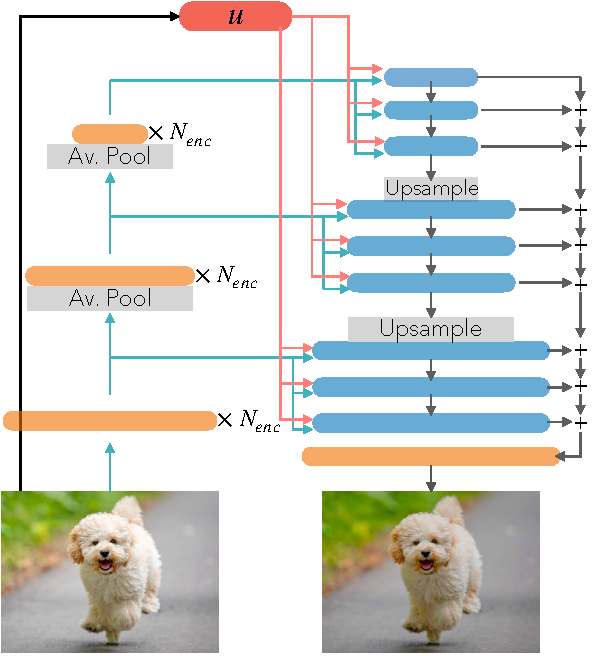
\includegraphics[width=0.51\linewidth]{pics/5_dvp/_full_model.pdf}}}
    &      
    \adjustbox{valign=b}{
        \begin{tabular}{@{}cc@{}}
        \multicolumn{2}{c}{
            \subfloat[Top down block\label{subfig:top_down}]{%
                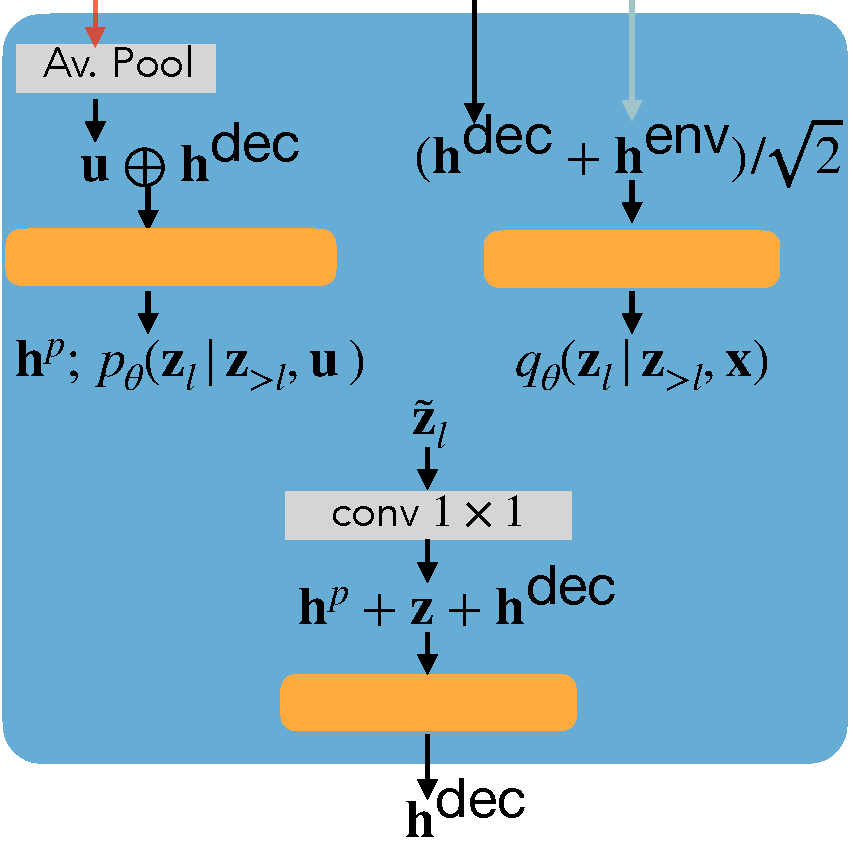
\includegraphics[width=.28\linewidth]{pics/5_dvp/_top_down_dct_2.pdf}}
        }\\
            \subfloat[Resnet block\label{subfig:resnet}]{%
                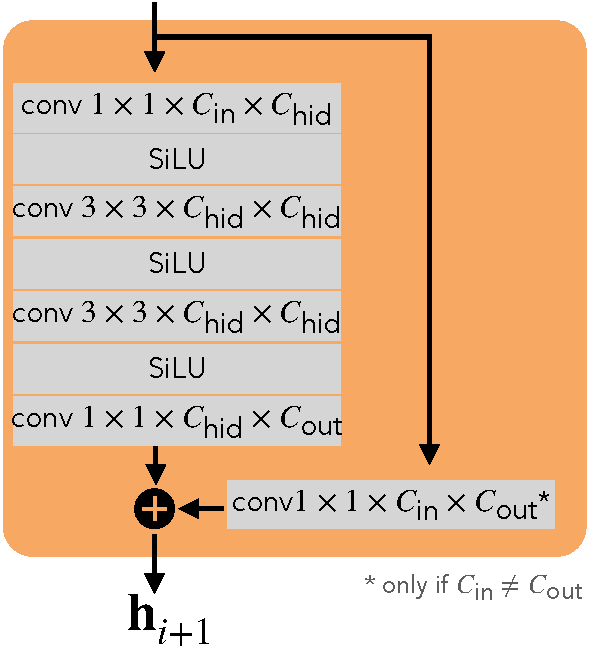
\includegraphics[width=.25\linewidth]{pics/5_dvp/_resnet_block.pdf}} &
            \subfloat[Pseudoinput block\label{subfig:context}]{%
                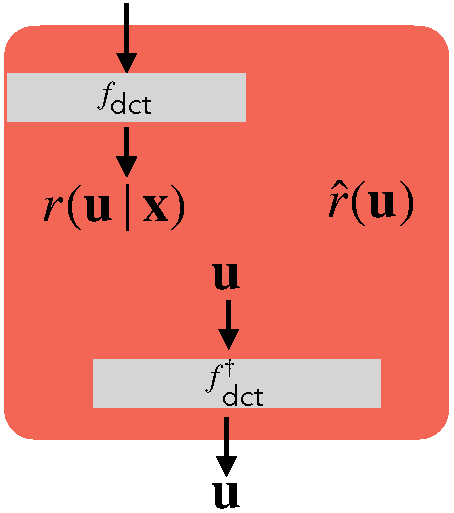
\includegraphics[width=.25\linewidth]{pics/5_dvp/_context_block.pdf}} \\
    \end{tabular}}
    \end{tabular}
    }
    % \caption[][\baselineskip]{A diagram of the DVP-VAE: TopDown hierarchical VAE with the diffusion-based VampPrior.\\
    %  (a) A \textit{BottomUp} path (left) and a \textit{TopDown} path (right). (b) A \textit{TopDown} block that takes features from the block above $\mathbf{h}^{dec}$, encoder features $\mathbf{h}^{enc}$ (only during training) and a pseudoinput $\rvu$ as inputs. (c) A single Resnet block. (d) A single pseudoinput block.
    % } 
    \captionsetup{width=1.3\textwidth, margin={0pt, -.3\textwidth}}
    \caption{A diagram of the DVP-VAE: TopDown hierarchical VAE with the diffusion-based VampPrior.
     (a) A \textit{BottomUp} path (left) and a \textit{TopDown} path (right). (b) A \textit{TopDown} block that takes features from the block above $\mathbf{h}^{dec}$, encoder features $\mathbf{h}^{enc}$ (only during training) and a pseudoinput $\rvu$ as inputs. (c) A single Resnet block. (d) A single pseudoinput block.
    } 
    \label{fig:model_schema}
    % \vskip 15pt
    \vskip -15pt
  \end{figure*}
  
The model architecture and parameterization are crucial to the scalability of the model. In this section, we discuss the specific choices we made.
The starting point for our architecture is the architecture proposed in VDVAE~\citep{Child2020-ze}. However, there are certain differences. We schematically depict our architecture in Figure~\ref{fig:model_schema}. We consider a hierarchical TopDown VAE with $L$ stochastic layers, namely, latent variables $\rvz_1, \dots, \rvz_L$. We assume that each latent variable has the same number of channels, but they differ in spatial dimensions: $\rvz_l \in \mathbb{R}^{c \times h_l \times w_l}$. We refer to different spatial dimensions of the latent space as \textit{scales}.

 \subsection{Bottom-up} \label{subsec:arch_encoder}
The bottom-up part corresponds to calculations of intermediary variables dependent on $\rvx$. We follow the implementation of \citet{Child2020-ze} for it. We start from the bottom-up path depicted in Figure~\ref{fig:model_schema}a (left), which is fully deterministic and consists of several ResNet blocks (see Figure~\ref{fig:model_schema}c)\citep{he2016deep}. 
The input is processed by $N_{\text{enc}}$ blocks at each scale, and the output of the last resnet block of each scale is passed to the TopDown path in Figure~\ref{fig:model_schema}a (right). Note that here $N_{\text{enc}}$ is a separate hyperparameter that does not depend on the number of stochastic layers $L$.
  

 \subsection{TopDown} \label{subsec:arch_decode}
The TopDown path depicted in Figure~\ref{fig:model_schema}a (right) computes the parameters of the variational posterior and the prior distribution starting from the top latent variable $\rvz_L$. 

The first step is the pseudoinput block shown in Figure~\ref{fig:model_schema}d. Using the deterministic function $f_{\text{dct}}$, it creates the pseudoinput random variable from the input $\rvx$ (see Algorithm~\ref{alg:context_forward}) that is used to train the Diffusion-based VampPrior $\hat{r}_{\gamma}(\rvu)$.
At test time, a pseudoinput is sampled using this unconditional prior. The pseudoinput sample is then converted back to the input domain (see Algorithm~\ref{alg:context_backward}) and used to condition prior distributions at all levels $p_{\theta}(\rvz_{1:L}|\rvu)$.

Next, the model has $L$ TopDown blocks depicted in Figure~\ref{fig:model_schema}b. 
Each TopDown block takes deterministic features from the corresponding scale of the bottom-up path denoted as $h_{\text{enc}}$, the output of the pseudoinput block $\rvu$, and deterministic features from the TopDown block above $h_{\text{dec}}$ as inputs. Our implementation of this block is similar to the VDVAE architecture, but there are several differences that we summarize below:
\begin{itemize}%[leftmargin=*]
    \item \textit{Incorporating pseudoinputs}\\
    We concatenate the pseudoinput (properly reshaped using average pooling) with $h_{\text{dec}}$ to compute the parameters of the prior distribution. 
    \item \textit{Variational posterior parameters} \\
    We assume that both $h_{\text{dec}}$ and $h_{\text{enc}}$ have the same number of channels, allowing us to sum them instead of concatenating. This reduces the total number of parameters and the memory consumption.
    \item \textit{Additional ResNet Connections}\\
    Our TopDown block has three ResNet blocks (Figure~\ref{fig:model_schema}c). In contrast to our architecture, in VDVAE only the block that updates $h_{\text{dec}}$ has a residual connection. 
\end{itemize}

We did not observe any training instabilities and did not apply the \textit{gradient skipping} used in \citet{Child2020-ze}.

 \subsection{Latent Aggregation in Conditional Likelihood} \label{subsec:latent_aggr}

% \paragraph{Latent Aggregation}
The last important element of our architecture is the \textit{aggregation of latents}. Let us denote samples from either the variational posteriors $q_{\phi}(\rvz_{1:L}|\rvx)$ during training or the prior $p_{\theta}(\rvz_{1:L}|\rvu)$ during generating new data as $\tilde{\rvz}_1, \dots, \tilde{\rvz}_L$.  
Furthermore, let $\vh_1$ be the output of the last TopDown block. 
These deterministic features are computed as a function of all samples $\tilde{\rvz}_1, \dots, \tilde{\rvz}_L$.
Therefore, it can be used to calculate the final likelihood value.
% \begin{align}\label{eq:cond_like_vdvae}
%     p_{\theta}(\rvx | \rvz_{1:L}) = p_{\theta}(\rvx | \text{Conv}(\vh_1)).
% \end{align}
However, we observe empirically that in such parameterization some layers of latent variables tend to be completely ignored by the model.
Instead, we propose to enforce a strong connection between the conditional likelihood and all latent variables by explicitly conditioning on all of the sampled latent variables, namely: 
\begin{align} \label{eq:cond_like_ours}
    p_{\theta}(\rvx | \rvz_{1:L}) = p_{\theta}\big( \rvx \big| \text{NN}\big(\frac{1}{\sqrt{L}}\sum\nolimits_l \tilde{\rvz}_l\big) \big).
\end{align}

We refer to this as the \textit{latent aggregation}.
We show empirically in the experimental section that this leads to a consistently high ratio of active units. 

 % \begin{table}
 %    % \begin{minipage}[c]{0.65\textwidth}
 %        \centering
 %        \caption{Differences between Very Deep VAE and DCT-VAE
 %        }
 %        \label{tab:main_results}
 %        \begin{tabular}{l| cc}
 %            \toprule
 %              & VDVAE & Ours\\
 %            \midrule
 %           Activation function & \\
 %            % Optimizer \\
 %            ResNet connections \\
 %            q\_net  \\
 %            Upsampling \\
 %            \bottomrule
 %        \end{tabular}% % \end{varwidth}%\hfill 
 % \end{table} 





%-------------------------------
% ==== SECTION: Related ====
%-------------------------------
\section{Related Work}
% \paragraph{Deep Hierarchical VAEs}
% \paragraph{VAE with VampPrior}
% \paragraph{Diffusion Prior in VAEs}
\paragraph{Latent prior in VAEs}
The original VAE formulation uses the standard Gaussian distribution as a prior over the latent variables.
This can be an overly simplistic choice, as the prior minimizing the Evidence Lower bound is given by the aggregated posterior \citep{hoffman2016elbo, tomczak2018vae}. 
Furthermore, using a unimodal prior with multimodal real-world data can lead to non-smooth encoder or meaningless distances in the latent space \citep{bozkurt2019rate}.
% \citet{bozkurt2019rate} study how rate-regularization affects VAE generalization and 
% Several prior works prosed to use more flexible prior distributions. 
More flexible prior distributions proposed in the literature include the Gaussian Mixture Model \citep{jiang2016variational, nalisnick2016approximate, tran2022cauchy}, the autoregressive normalizing flow \citep{chen2016variational}, the autoregressive model \citep{gulrajani2016pixelvae, sadeghi2019pixelvae++}, the rejection sampling distribution with the learned acceptance function \citep{bauer2019resampled}, the diffusion-based prior \citep{vahdat2021score, wehenkel2021diffusion}. The VampPrior \citep{tomczak2018vae} proposes using an approximation of the aggregated posterior as a prior distribution. The approximation is constructed using learnable pseudoinputs to the encoder.
This work can be seen as an efficient extension of the VampPrior to deep hierarchical VAE, which also utilizes a diffusion-based prior over the pseudoinputs. 

\paragraph{Auxiliary Variables in VAEs}

Several works consider auxiliary variables $\rvu$ as a way to improve the flexibility of the variational posterior.
\citet{maaloe2016auxiliary} use auxiliary variables with one-level VAE to improve the variational approximation while keeping the generative model unchanged. 
\citet{salimans2015markov} use Markov transition kernel for the same expressivity purpose. The authors treat intermediate MCMC samples as an auxiliary random variable and derive evidence lower bound of the extended model. 
\citet{ranganath2016hierarchical} introduce hierarchical variational models. They increase the flexibility of the variational approximation by imposing prior on its parameters. 
In this setting, it assumes that the latent variable $\rvz$ and the auxiliary variable $\rvu$ are not conditionally independent and the variational posterior factorizes, for example, as follows:
\begin{equation}
    q_{\phi}(\rvu, \rvz|\rvx) = q_{\phi}(\rvu|\rvx)q_{\phi}(\rvz|\rvu, \rvx).
\end{equation}
In this work, in contrast, we use auxiliary variable to increase the prior flexibility and use conditional independence assumption in the variational posterior:
\begin{equation}
    q_{\phi}(\rvu, \rvz|\rvx) = q_{\phi}(\rvu|\rvx)q_{\phi}(\rvz|\rvx).
\end{equation}

\citet{khemakhem2020variational} consider the non-identifiability problem of VAEs. They propose to use auxiliary observation $\rvu$ and use it to condition the prior distribution. This additional observation is similar to the pseudoinputs that we consider in our work. However, we define a way to construct $\rvu$ from the input and learn a prior distribution to sample it during inference, while \citet{khemakhem2020variational} require $\rvu$ to be observed both during training and at the inference time.

Similarly to our work, \citet{klushyn2019learning} consider the hierarchical prior $p_{\theta}(\rvz|\rvu)p(\rvu)$. However, they treat $\rvu$ rather as a second layer of latent variables and learn a variational posterior in the form $q_{\phi}(\rvu, \rvz|\rvx) = q_{\phi}(\rvu|\rvz)q_{\phi}(\rvz|\rvx)$. 

\paragraph{Latent Variables Aggregation}
There are different ways in which the conditional likelihood $p_{\theta}(\rvx|\rvz_{1:L})$ can be parameterized. In LadderVAE \citep{sonderby2016ladder}, where TopDown hierarchical VAE was originally proposed, the following formulation is used:
\begin{equation}
    p_{\theta}(\rvx|\rvz_{1:L}) = p_{\theta}(\rvx|\text{NN}(\rvz_{1})).
\end{equation}
That is, the conditional likelihood depends directly on the bottom latent variable $\rvz_{1}$ only. 

Later, NVAE \citep{vahdat2020nvae} and VDVAE \citep{Child2020-ze} use a deterministic path in the TopDown architecture in the conditional likelihood, namely:
\begin{equation}\label{eq:cond_like_vdvae}
    p_{\theta}(\rvx|\rvz_{1:L}) = p_{\theta}(\rvx|\text{NN}(\rvh_1)).
\end{equation}
Note that deterministic features depend on all the latent variables. However, we propose to use a more explicit dependency on latent variables in Eq.~\ref{eq:cond_like_ours}. Our idea bears some similarities with Skip-VAE \citep{dieng2019avoiding}. Skip-VAE proposes to add a latent variable to each layer of the neural network parameterizing decoder of the VAE with a single stochastic layer. In this work, instead, we add all the latent variables together to parameterize conditional likelihood. 


%-------------------------------
% ==== SECTION: Experiments ====
%-------------------------------

%----SECTION----
% \newpage
\section{Experiments}


%----SECTION----
\subsection{Settings}
We evaluate DVP-VAE on dynamically binarized MNIST \citep{lecun1998mnist} and OMNIGLOT \citep{lake2015human}. Furthermore, we conduct experiments on natural images using the CIFAR10 dataset \citep{Krizhevsky09learningmultiple}. We provide all the hyperparameters for training DVP-VAE in Appendix \ref{appendix:hyperparams} and in the code repository\footnote{\url{github.com/AKuzina/dvp_vae}}.
%----SECTION----
\subsection{Main Quantitative and Qualitative Results}\label{sect:exp_image_generations}

 \begin{table}[t]
        \centering
        \caption{The test performance: negative log likelihood on MNIST and OMNIGLOT, and bits-per-dimension (BPD) on CIFAR10.\\
        \textsuperscript{$\ddagger$} Results with data augmentation.\\
        \textsuperscript{$*$} Results averaged over 4 random seeds. Standard deviation reported in parentheses. 
        }
        \label{tab:main_results}
        \small{
        \begin{tabular}{l||lll|lll}
            \toprule
            \multirow{2}{*}{\textsc{Model}} & \multirow{2}{*}{\small{\textsc{L}}} & \footnotesize{\textsc{MNIST}} & \footnotesize{\textsc{OMNIGLOT}} & \multicolumn{3}{c}{\footnotesize{\textsc{CIFAR10}}}\\ 
                & &  \multicolumn{2}{c|}{$ - \log p(\rvx) \leq \, \downarrow $} & \small{\textsc{Size}} & \small{\textsc{L}} & \small{\textsc{bpd $ \leq \, \downarrow $}}\\
            \midrule
            \textbf{DVP-VAE} \normalsize{(ours)} & 8 
                    & \textbf{77.10}$^*$\footnotesize{(0.05)} & \textbf{89.07}$^*$\footnotesize{(0.10)}  
                    & 20M & 28 & \textbf{2.73}\\
            Attentive VAE \small{\citep{apostolopoulou2021deep}}  & \multirow{1}{*}{15}
                    & \multirow{1}{*}{77.63} & \multirow{1}{*}{89.50} & 119M & 16 & 2.79\\
            CR-NVAE \small{\citep{sinha2021consistency}}               & \multirow{1}{*}{15}
                    & \multirow{1}{*}{76.93\textsuperscript{$\ddagger$}} & \multirow{1}{*}{---} & 131M & 30 & 2.51\textsuperscript{$\ddagger$} \\
            VDVAE \small{\citep{Child2020-ze}} & --- & --- & --- & 39M & 45& 2.87 \\
            OU-VAE \small{\citep{pervez21a}} & \multirow{1}{*}{5}
                    & \multirow{1}{*}{81.10} & \multirow{1}{*}{96.08}         
                    & 10M & 3 & 3.39 \\
                    % \small{\citep{pervez21a}} \\
            NVAE \small{\citep{vahdat2020nvae}}& \multirow{1}{*}{15}
                    & \multirow{1}{*}{78.01} & \multirow{1}{*}{---} 
                    & --- & 30 & 2.91 \\
            BIVA\small{\citep{maaloe2019biva}}   & 6
                    & 78.41 & 91.34 & 103M & 15 & 3.08 \\
            VampPrior \small{\citep{tomczak2018vae}} & \multirow{1}{*}{2}
                    & \multirow{1}{*}{78.45}  &   \multirow{1}{*}{89.76}             
                    & --- & --- & --- \\
            LVAE \small{\citep{sonderby2016ladder}} & \multirow{1}{*}{5}
                    & \multirow{1}{*}{81.74} & \multirow{1}{*}{102.11}     
                    & --- & --- & --- \\
            IAF-VAE\small{\citep{kingma2016improved}} & \multirow{1}{*}{---}
                    & \multirow{1}{*}{79.10}  &   \multirow{1}{*}{---}             
                    & --- & 12 & 3.11 \\
            % \midrule
            % & \multicolumn{6}{c}{\footnotesize{Diffusion models}}\\
            % Improved DDPM \citep{nichol2021improved} &  --- & --- & --- &  & & 2.94 \\
            % VDM \citep{kingma2021variational} &  --- & --- & --- &  & & 2.64\\
            % DiffEnc \citep{nielsendiffenc} &  --- & --- & --- &  & & 2.62\\
            % NDM \citep{bartosh2023neural}&  --- & --- & --- &  & & 2.70\\
            \bottomrule
        \end{tabular}% % \end{varwidth}%\hfill 
        \vskip 10pt
        }
 \end{table} 
We report all results in Table \ref{tab:main_results}, where we compare the proposed approach with other hierarchical VAEs. 
We observe that DVP-VAE outperforms most of the VAE models\footnote{CR-NVAE \citep{sinha2021consistency} uses NVAE model and considerably improves its performance by applying data augmentations. We did not use any augmentations to compare fairly with all other hierarchical VAEs and were able to get a better NLL than NVAE and more recent hierarchical VAE models.
} while using fewer parameters than other models. For instance, on CIFAR10, our DVP-VAE requires 20M weights to beat Attentive VAE with about 6 times more weights.
Furthermore, because of the smaller model size, we were able to obtain all the results using a single GPU. 
We show the unconditional samples in Figure~\ref{fig:dct_samples} (see Appendix~\ref{appendix:samples} for more samples). 
The top row of each image shows samples from the diffusion-based VampPrior (i.e., pseudoinputs), while the second row shows corresponding samples from the VAE. 
We observe that, as expected, pseudoinputs define the general appearance of an image, while a lot of details are added later by the TopDown decoder. 
This effect can be further observed in Figure~\ref{fig:generative_recon} where we plot the reconstructions using different numbers of latent variables. In the first row, only a pseudoinput corresponding to the original image is used (i.e., $\rvu \sim r(\rvu|\rvx)$) while the remaining latent variables are sampled from the prior with low temperature. Each row below uses more latent variables from the variational posterior grouped by the scales. 
Namely, the second row uses the pseudoinput above and all the $4\times4$ latent variables from the variational posterior, then the third row uses additionally $8\times8$ latent variables, and so on. 

 \begin{figure}[t]
 \begin{center}
    \begin{tabular}{c}
        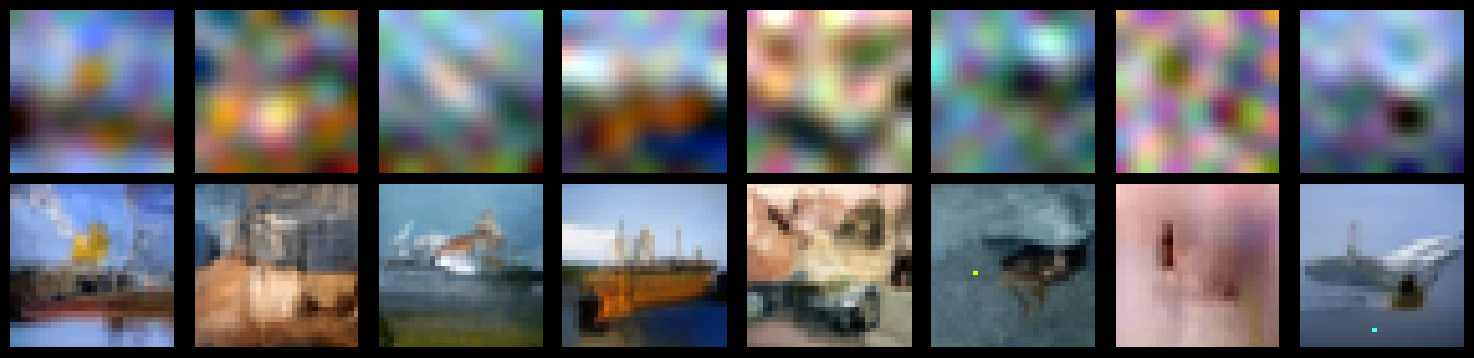
\includegraphics[width=0.5\textwidth]{pics/5_dvp/cifar10_dct_prior_samples.pdf} \\
        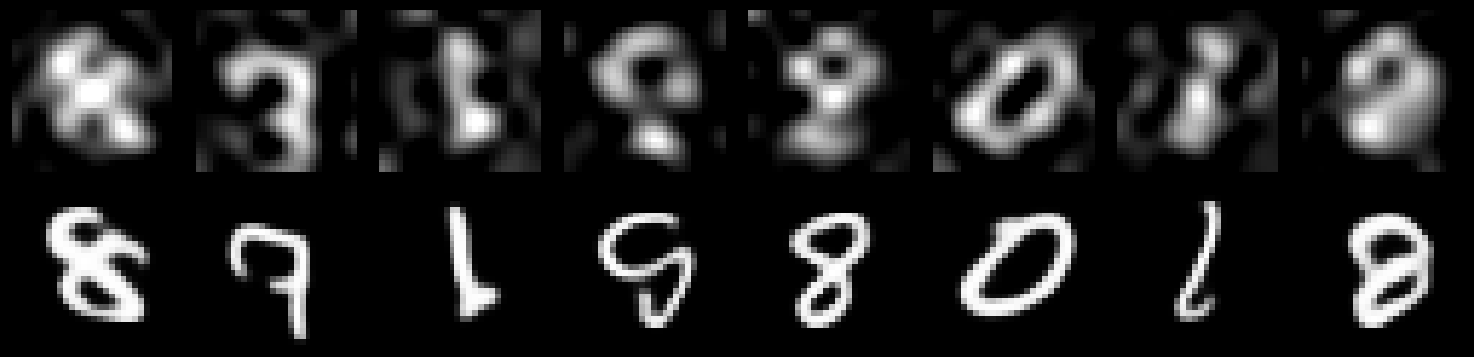
\includegraphics[width=0.5\textwidth]{pics/5_dvp/mnist_dct_prior_samples.pdf} \\
        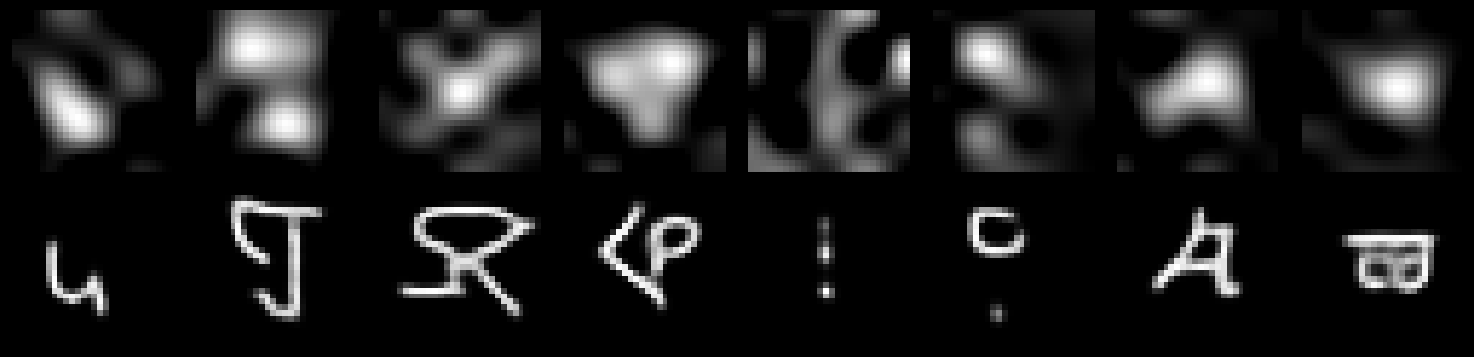
\includegraphics[width=0.5\textwidth]{pics/5_dvp/omniglot_dct_prior_samples.pdf} \\
    \end{tabular}
    \end{center}
    \caption{Unconditional samples from the Diffusion-based VampPrior (top) and corresponding samples from the DVP-VAE (bottom).}
    \label{fig:dct_samples}
    \vskip 20pt
\end{figure}

\begin{figure}[t]
\begin{center}
    \begin{tabular}{cc}
        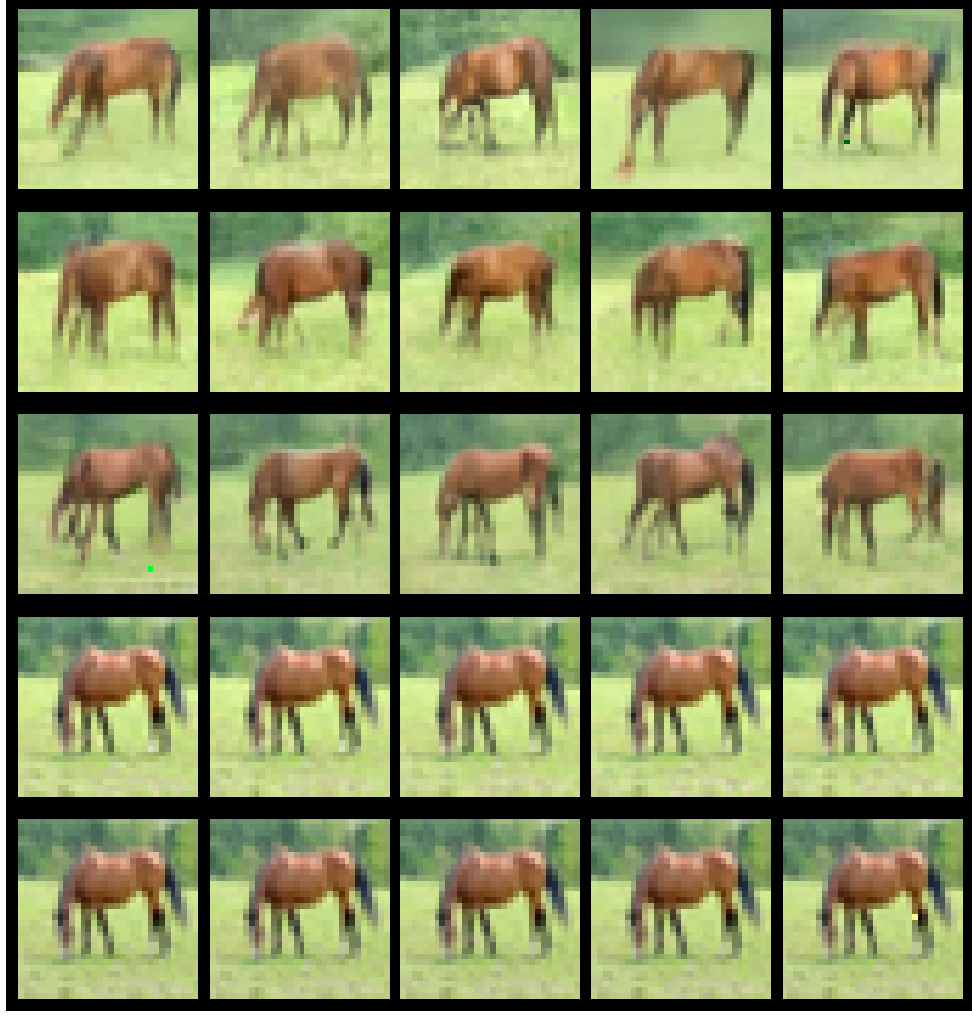
\includegraphics[width=0.4\textwidth]{pics/5_dvp/cifar10_generative_rec_6.pdf} &
        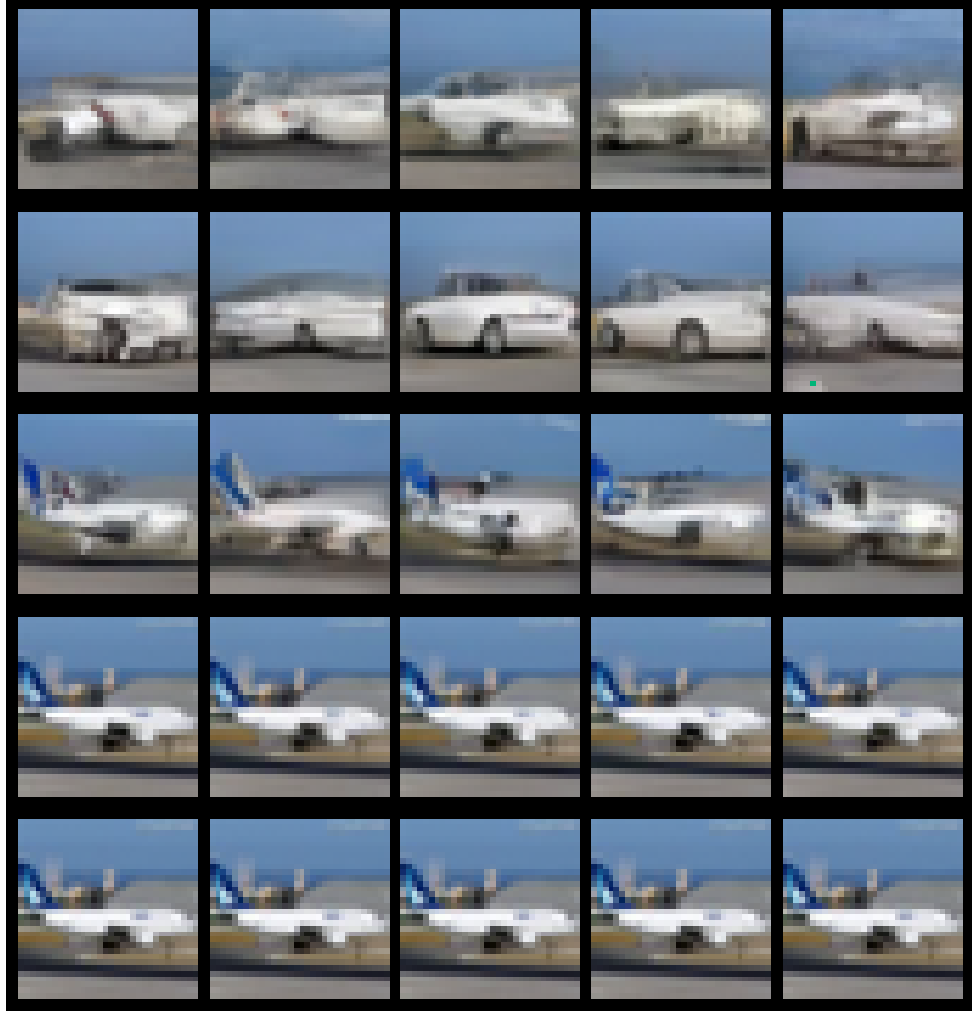
\includegraphics[width=0.4\textwidth]{pics/5_dvp/cifar10_generative_rec_9.pdf} \\ 
    \end{tabular}
\end{center}
    \caption{\textit{Generative reconstruction}s. The top row is using a pseudoinput sampled from $r(\rvu|\rvx)$ \textbf{only}.}
    \label{fig:generative_recon}
    \vskip 10pt
\end{figure}
% \begin{table}[t]
% \begin{minipage}[t]{0.45\linewidth}
% \begin{figure}[H]
%     \begin{tabular}{c}
%         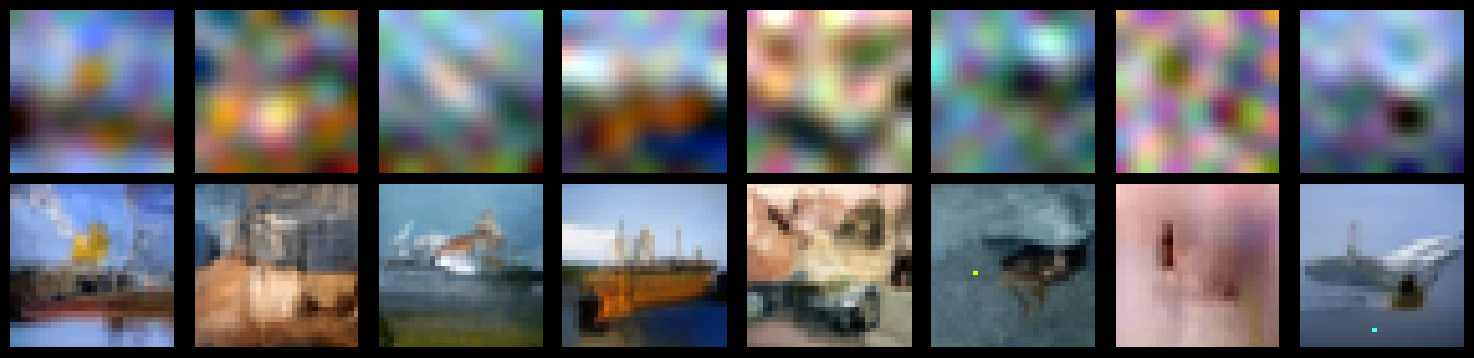
\includegraphics[width=0.85\textwidth]{pics/5_dvp/cifar10_dct_prior_samples.pdf} \\
%         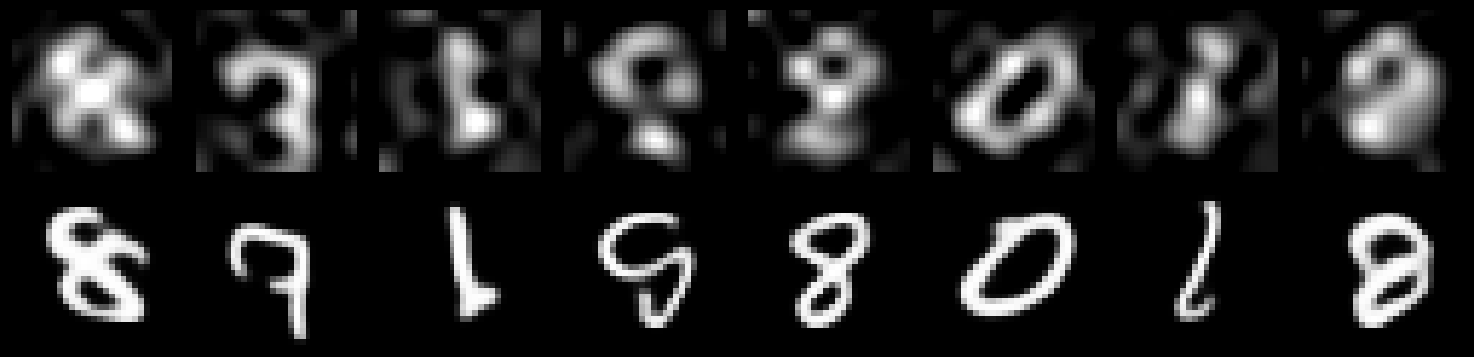
\includegraphics[width=0.85\textwidth]{pics/5_dvp/mnist_dct_prior_samples.pdf} \\
%         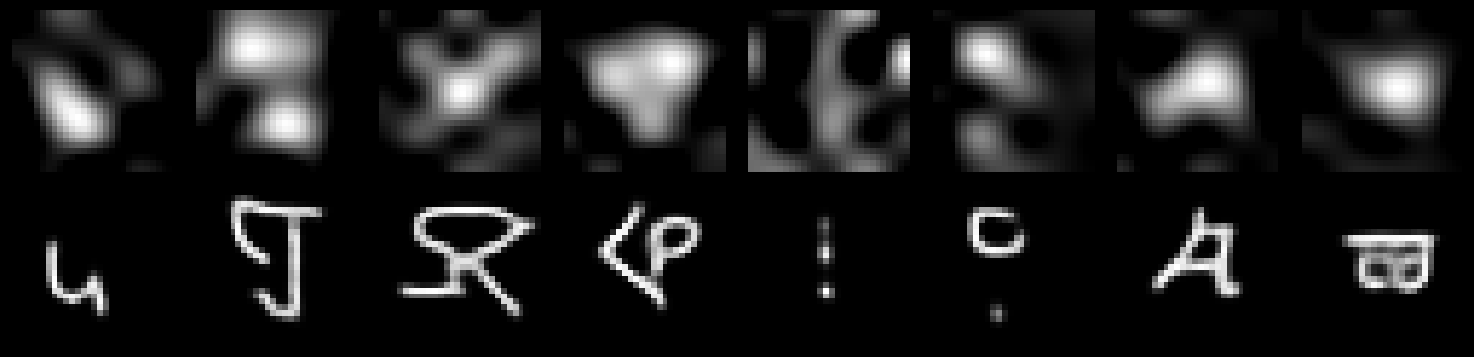
\includegraphics[width=0.85\textwidth]{pics/5_dvp/omniglot_dct_prior_samples.pdf} \\
%     \end{tabular}
%     \caption{Unconditional samples from the Diffusion-based VampPrior (top) and corresponding samples from the DVP-VAE (bottom).}
%     \vskip -5pt
%     \label{fig:dct_samples}
% \end{figure}
% \end{minipage}\hfill
% \begin{minipage}[t]{.65\linewidth}
% \begin{figure}[H]
%     \begin{tabular}{cc}
%         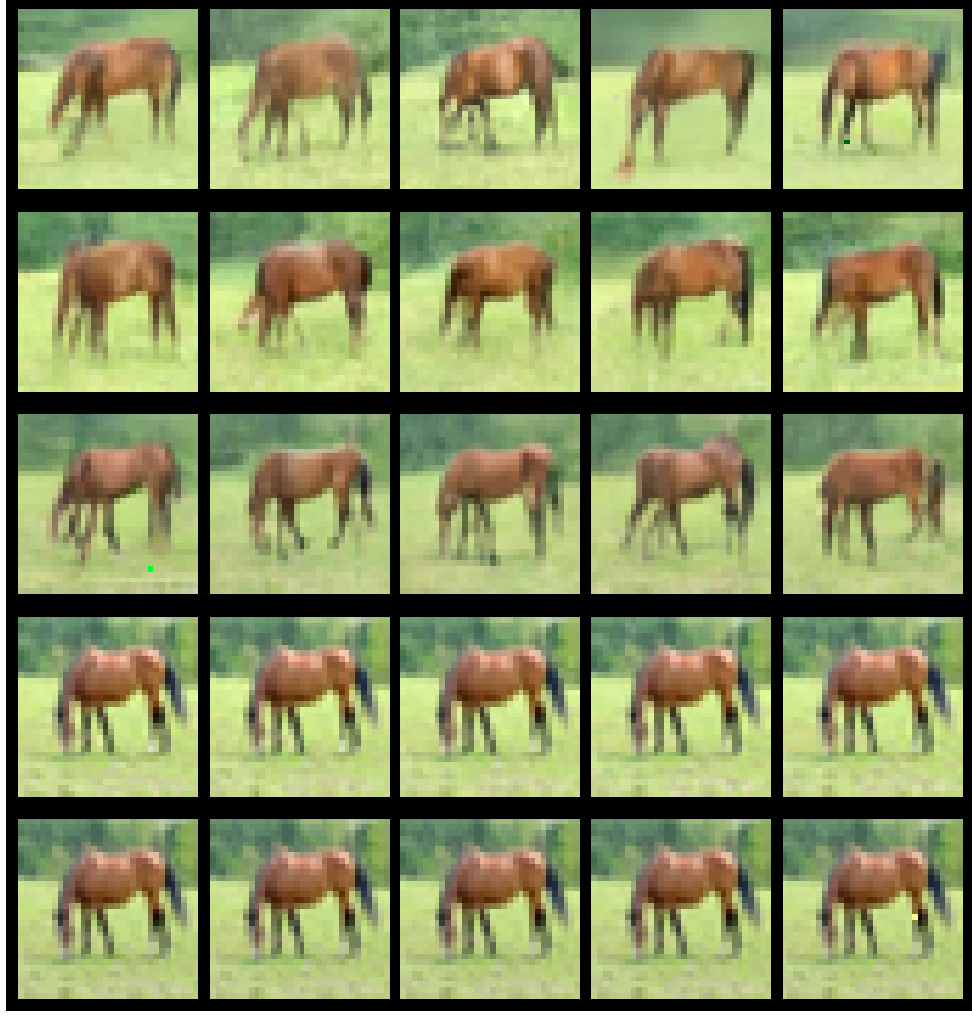
\includegraphics[width=0.43\textwidth]{pics/5_dvp/cifar10_generative_rec_6.pdf} &
%         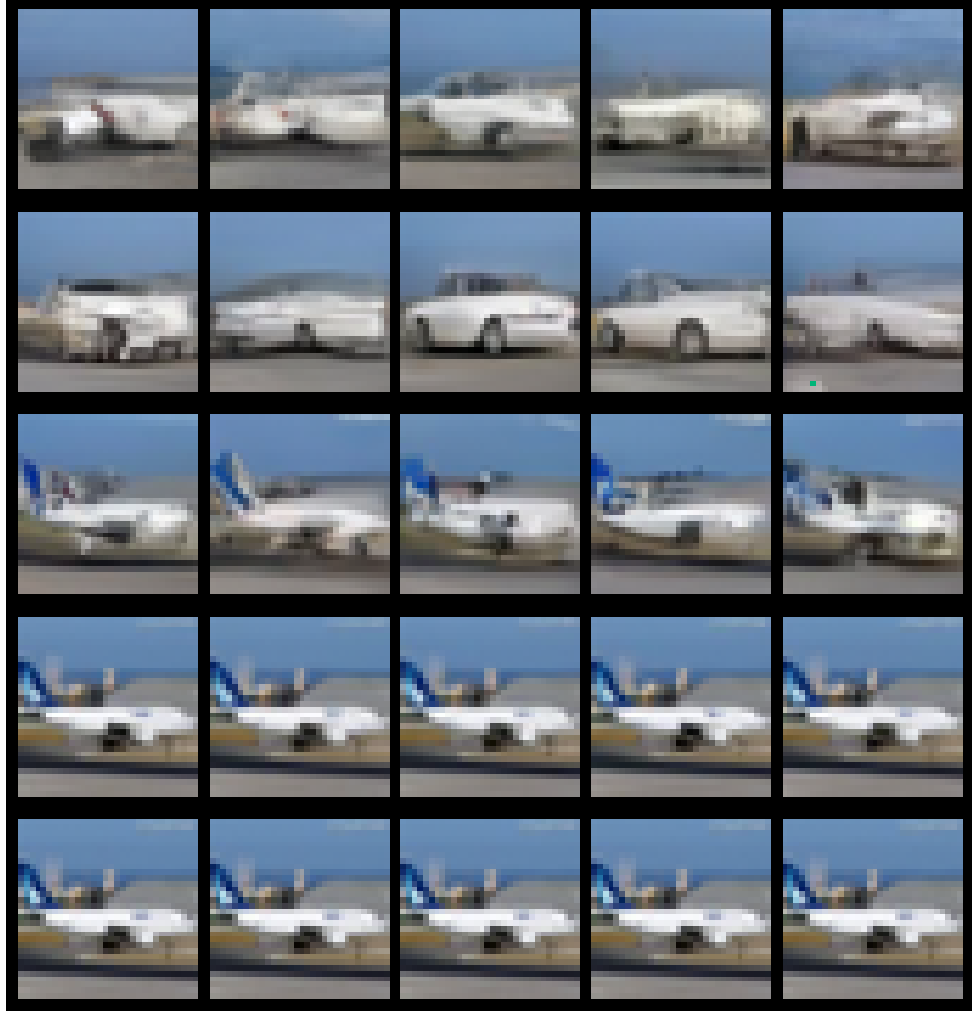
\includegraphics[width=0.43\textwidth]{pics/5_dvp/cifar10_generative_rec_9.pdf} \\ 
%     \end{tabular}
%     \caption{\textit{Generative reconstruction}s. The top row is using a pseudoinput sampled from $r(\rvu|\rvx)$ \textbf{only}.}
%     \vskip -5pt
%     \label{fig:generative_recon}
% \end{figure}
% \end{minipage}\hfill
% \end{table}



%%%%%%%%%%%%%%%%% POSTERIOR COLLAPSE %%%%%%%%%%%%%%%%%

%----SECTION----
\subsection{Ablation Studies}\label{sect:ablation}


\paragraph{Training stability and convergence}

% We employ severla changes in the architecture, which were made to improve training stability. 

In all of our experiments, we did not observe many training instabilities. 
Unlike many contemporary VAEs, we did not use gradient skipping \citep{Child2020-ze}, spectral normalization \citep{vahdat2020nvae}, or softmax parameterization of variances \citep{hazami2022efficientvdvae}. 
We use the Adamax version of the Adam optimizer \citep{kingma2015adam} following \citet{hazami2022efficientvdvae}, as it demonstrated much better convergence for the model with a mixture of discretized logistic likelihood. 

First, we observe a consistent performance improvement as we increase the model size and the number of stochastic layers. 
In Table~\ref{tab:increase_num_layers}, we report test performance and the percentage of active units (see Section~\ref{subsec:active_units} for details) for models of different stochastic depths trained on the CIFAR10 dataset. 
We train each model for 500 epochs, which corresponds to less than 200k training iterations. 
Additionally, we report gradient norms and training and validation losses for all four models in Appendix~\ref{appx:depth_experiment}. 


To demonstrate the advantage of the proposed architecture, we compare our model to a closest deep hierarchical VAE architecture: Very Deep VAE. For this experiment, we chose hyperparameters closest to Table 4 in \cite{Child2020-ze} (CIFAR-10). That is, our model has 45 stochastic layers and a comparable number of trainable parameters. Furthermore, following \cite{Child2020-ze}, we train this model with a batch size of 32, a gradient clipping threshold of 200, and an EMA rate of 0.9998. 
% We trained a model with the same number of stochastic layers (45) and similar number of parameters. 
% We used the same batch size (32) and gradient clipping (200). 
However, in DVP-VAE, we were able to eliminate gradient skipping and gradient smoothing. 
We report the difference in key hyperparameters and test performance in Table \ref{tab:ablation_stability}. We also add a comparison with Efficient-VDVAE (see Table 3 in \cite{hazami2022efficientvdvae}).
We observe that DVP-VAE achieves comparable performance within much fewer training iterations than both VDVAE implementations. 

\begin{table}[t]
    \centering
    \caption{Test performance for the model trained for 500 epochs (or approximately 200k training iterations) on CIFAR10.}    \label{tab:increase_num_layers}
    \begin{tabular}{ll|cc}
        \toprule
         \textsc{L} & \textsc{Size} & \textsc{BPD}$\leq$ $\downarrow$ & \textsc{AU} $\uparrow$\\
        \midrule
        20 & 24M & 2.99 & 94\%\\
        28 & 32M & 2.94 & 93\% \\
        36 & 40M & 2.89 & 98\%\\
        44 & 48M & 2.84 & 97\%\\
        \bottomrule
    \end{tabular}
    \vskip 20pt
\end{table}

% \begin{table*}[t]
% \begin{minipage}[t]{.3\linewidth}
%     \centering
%     \captionof{table}{Test performance for the model trained for 500 epochs (or approximately 200k training iterations) on CIFAR10.}    \label{tab:increase_num_layers}
%     \begin{tabular}{ll|cc}
%         \toprule
%          \textsc{L} & \textsc{Size} & \textsc{BPD}$\leq$ $\downarrow$ & \textsc{AU} $\uparrow$\\
%         \midrule
%         20 & 24M & 2.99 & 94\%\\
%         28 & 32M & 2.94 & 93\% \\
%         36 & 40M & 2.89 & 98\%\\
%         44 & 48M & 2.84 & 97\%\\
%         \bottomrule
%     \end{tabular}
%     \vskip -25pt   
% \end{minipage}\hfill
% \begin{minipage}[t]{.67\linewidth}
\begin{table}[t]
    \centering
    \captionof{table}{Training settings for the model trained on CIFAR-10 compared to two VDVAE implementations. 
    }
    \label{tab:ablation_stability}
    % \small{
    \begin{tabular}{l|ccc}
        \toprule
         & \small{\textsc{VDVAE}} & \small{\textsc{Efficient-VDVAE}} &\small{\textsc{DVP-VAE}} \\
         & \footnotesize{\citep{Child2020-ze}} & \footnotesize{\citep{hazami2022efficientvdvae}}&\footnotesize{(ours)}\\
        \midrule
        \textsc{L} & 45 & 47 & 45 \\
        \textsc{Size} & 39M & 57M & 38M \\
        % Batch size & 32 & 16 & 32\\
        \textsc{Optimizer} & \textsc{AdamW} & \textsc{Adamax} & \textsc{Adamax}\\
        \textsc{Learning rate} & 2e-4 & 1e-3 & 1e-3\\
        % \textsc{Weight decay} & 1e-2 & &1e-6\\
        \textsc{Grad. smoothing} & -- & Yes & --\\
        \textsc{Grad. skip} & 400 & 800 & --\\
        % Grad. clip & 200 & 200\\
        % EMA rate & 0.9998 & 0.9998\\
        \textsc{Training iter.} & 1.1M & 0.8M &\textbf{0.4M} \\
        % \small{GPUs}  & 2$\times$V100 & 1$\times$A100\\
        % \small{Training time} & 6 days & \ak{$\sim$ 5 days}\\
        \midrule
        \textsc{Test BPD} & 2.87 & 2.87 &2.86 \\
        \bottomrule
    \end{tabular}
    \vskip 20pt
    % }
    % \vskip -30pt   
% \end{minipage}
\end{table}


\paragraph{Latent Aggregation Increases Latent Space Utilization}\label{subsec:active_units}

Next, we test the claim that latent variable aggregation discussed in Sec.~\ref{subsec:latent_aggr} improves latent space utilization. We use Active Units (AU) metric~\citep{burda2015importance}, which can be calculated for a given threshold $\delta$ as follows:
\begin{align}\label{eq:active_units}
\text{AU} &= \frac{\sum_{l=1}^L \sum_{i=1}^{M_l}  \left[\text{A}_{l, i} > \delta \right] }{\sum_{l=1}^L M_l }, \\
    \text{where } \text{A}_{l} &= \text{Var}_{q^{\text{test}}(\rvx)} \E_{q_{\phi}(\rvz_{l+1:L}|\rvx)} \E_{q_{\phi}(\rvz_l | \rvz_{l+1:L}, \rvx)}\left[\rvz_l\right].
\end{align}
Here $M_{l}$ is the dimensionality of the stochastic layer $l$, $\left[ B \right]$ is the Iverson bracket, which equals $1$ if $B$ is true and $0$ otherwise, and $\text{Var}$ stands for variance.
Following \citet{burda2015importance}, we use the threshold $\delta = 0.01$. The higher the share of active units, the more efficient the model is in utilizing its latent space. 

We report results in Table~\ref{tab:ablation_active_units} and observe that the model with latent aggregation always attains more than 90\% of active units. Furthermore, latent aggregation considerably improves the utilization of the latent space if we compare it with exactly the same model but with the conditional likelihood parameterized using deterministic feature from the TopDown path (see Eq.~\ref{eq:cond_like_vdvae}).
\begin{table*}[t]
\begin{minipage}[t]{.49\linewidth}
   \centering
       \captionof{table}{Active Units for the DCT-VAE with and without latent aggregation. 
       }
    \label{tab:ablation_active_units}
    \small{
    \begin{tabular}{ccc|c}
        \toprule
             \footnotesize{\textsc{Latent Aggr.}}& \footnotesize{\textsc{Size}} &
             \footnotesize{\textsc{L}} & \footnotesize{\textsc{AU}} $\uparrow$  \\
            \midrule
                \multicolumn{3}{c}{\footnotesize{\textsc{MNIST}}} \\
            \midrule
          \ding{55}   & 0.7M & 8 & 33.2\%\\
          $\checkmark$& 0.7M & 8 & 91.5\%\\
        \midrule
                \multicolumn{3}{c}{\footnotesize{\textsc{OMNIGLOT}}} \\
            \midrule
         \ding{55}    & 1.3M & 8 & 71.3\%\\
         $\checkmark$ & 1.3M & 8 & 93.4\%\\
         \midrule
                \multicolumn{3}{c}{\footnotesize{\textsc{CIFAR10}}} \\
            \midrule
         $\checkmark$    &  19.5M & 28 & 98\%\\
        \bottomrule
    \end{tabular}
    }
\end{minipage}\hfill
\begin{minipage}[t]{0.49\linewidth}
\centering
      \captionof{table}{Test NLL for the model with and without pseudoinputs. Averaged over 4 random seeds, standard deviation in parenthesis.}
    % \vskip 5pt
    \label{tab:ablation_nll}
    \small{
    \begin{tabular}{cc|c}
        \toprule
              \footnotesize{\textsc{Pseudoinputs}} & \footnotesize{\textsc{Size}} & \footnotesize{\textsc{NLL}}$\downarrow$  \\
            \midrule
                \multicolumn{3}{c}{\footnotesize{\textsc{MNIST}}} \\
            \midrule
        \ding{55}    & \footnotesize{0.6M} & 78.85 \footnotesize{(0.24)} \\
        $\checkmark$ & \footnotesize{0.7M} & 77.10  \footnotesize{(0.05)}\\ 
        \midrule
        \multicolumn{3}{c}{\footnotesize{\textsc{OMNIGLOT}}} \\
        \midrule
         \ding{55} & \footnotesize{1.1M} & 89.52 \footnotesize{(0.23)}\\
     $\checkmark$  & \footnotesize{1.3M} & 89.07 \footnotesize{(0.10)}\\
        \bottomrule
    \end{tabular}
    }
\end{minipage}
\end{table*}


\begin{figure}[t]
    \begin{tabular}{cc}
        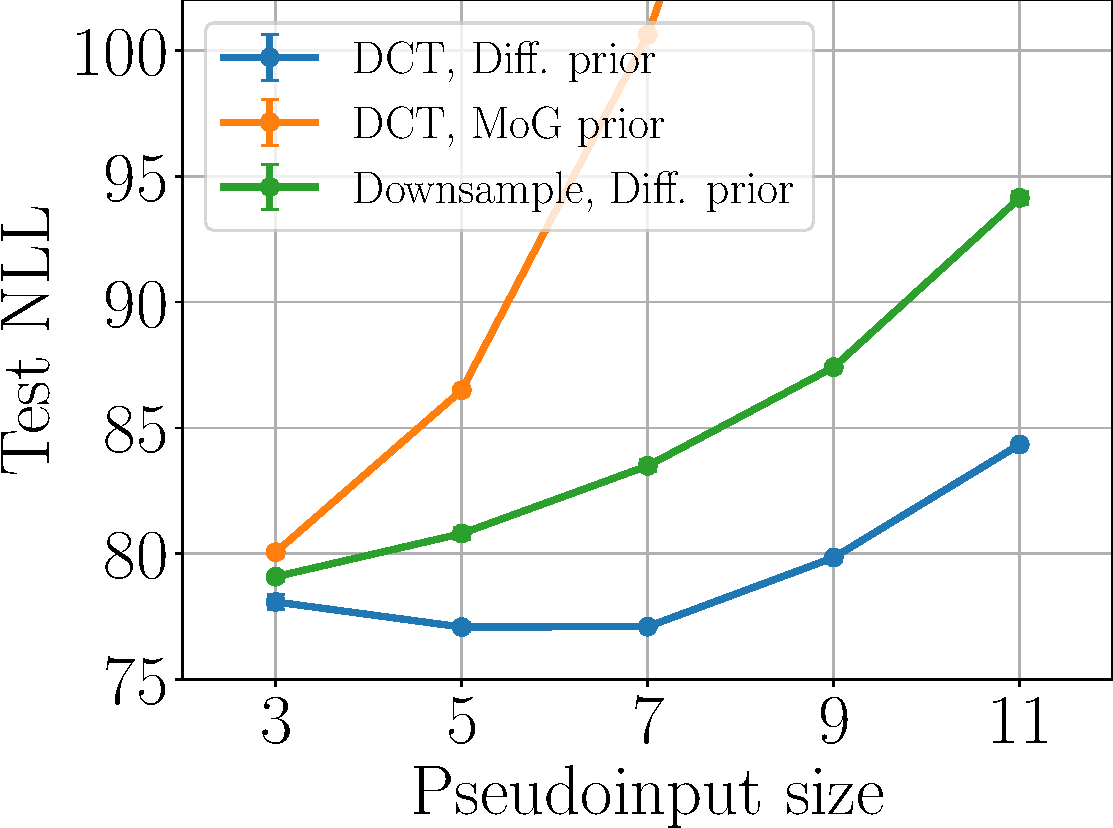
\includegraphics[width=0.43\linewidth]{pics/5_dvp/mnist_ctx_ablaions_line.pdf} &
        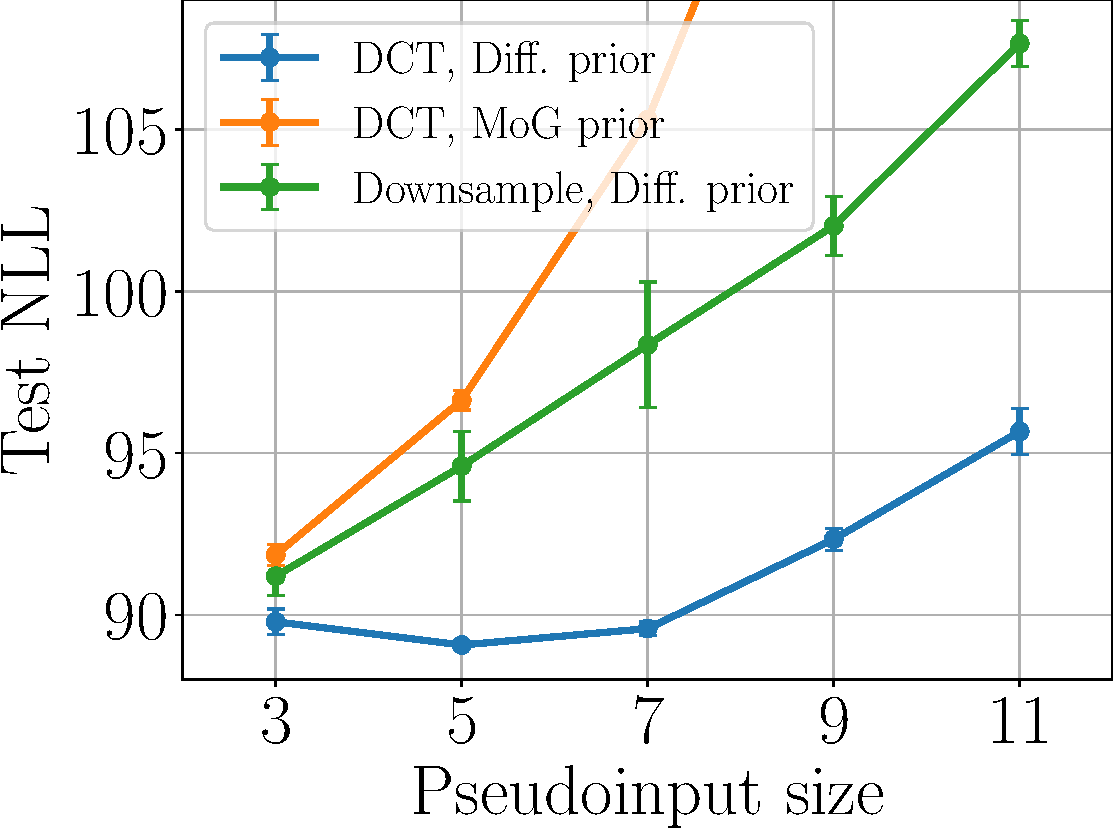
\includegraphics[width=0.43\linewidth]{pics/5_dvp/omniglot_ctx_ablaions_line.pdf} \\
        (a) MNIST &
        (b) OMNIGLOT \\
    \end{tabular}
    \caption{Ablation study of for the pseudoinputs type (DCT and Downsampled image), pseudoinputs prior (Diffusion model and Mixture of Gaussians) and pseudoinputs size (ranging from $3\times 3$ to $11\times 11$). Each configuration is trained with four different random seeds.}
    \label{fig:mnist_ctx_ablations}
    \vskip 10pt
\end{figure}

\begin{figure}[t]
    \begin{tabular}{cc}
        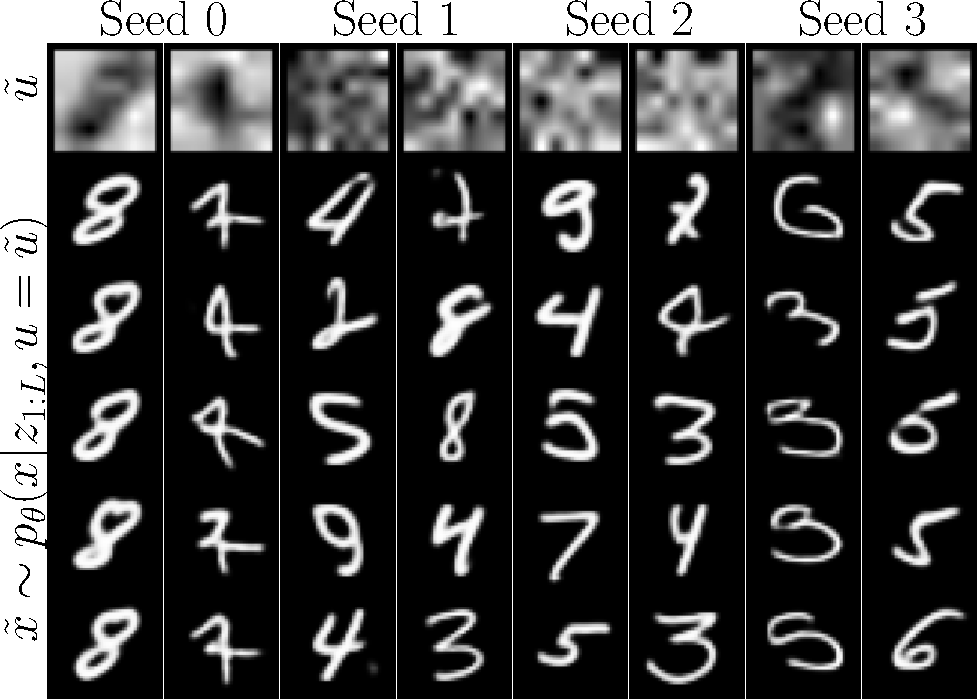
\includegraphics[width=0.43\textwidth]{pics/5_dvp/mnist_linear_prior_samples.pdf} &
        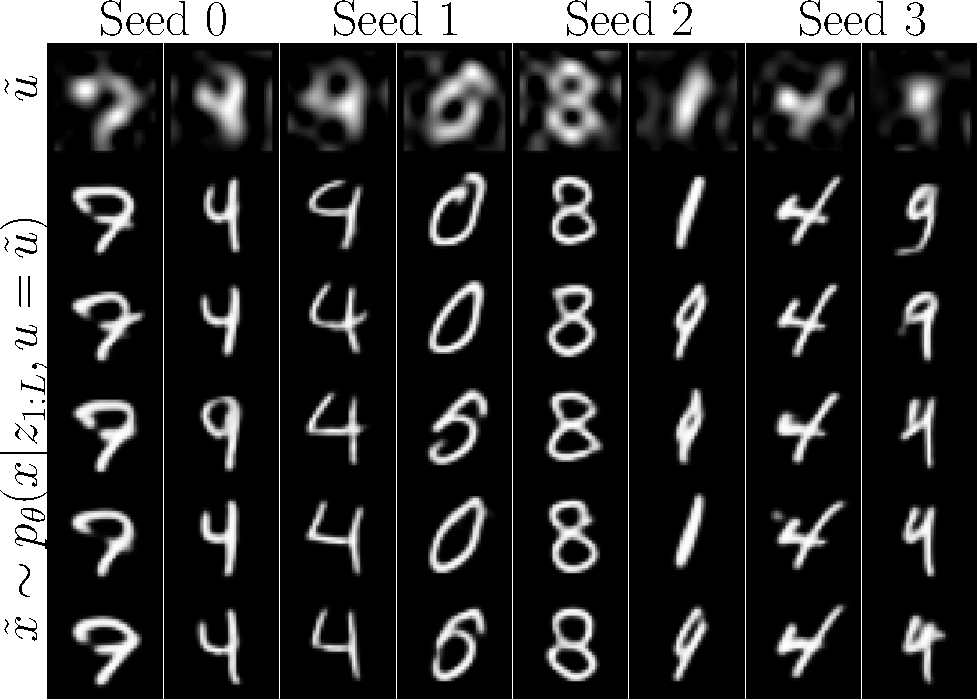
\includegraphics[width=0.43\textwidth]{pics/5_dvp/mnist_dct_prior_samples_seed.pdf} \\ \\
        (a) Learnable pseudoinputs &
        (b) DCT pseudoinputs \\
    \end{tabular}
    \caption[][\baselineskip]{Samples from the pseudoinputs prior $\Tilde{\rvu} \sim \hat{r}(\rvu)$ (top row) and corresponding samples from the model $\Tilde{\rvx} \sim p_{\theta}(\rvx|\rvz_{1:L}, \rvu=\Tilde{\rvu})$ (other rows). Columns corresponds to models trained with different random seeds.}
    \label{fig:linear_context_sampels}
    \vskip 10pt
\end{figure}


\paragraph{Amortized VampPrior Improves BPD}

Further, we test how the proposed amortized VampPrior improves model performance as measured by the negative log-likelihood. We report results in Table~\ref{tab:ablation_nll} and observe that DVP-VAE always has a better NLL metric compared to the deep hierarchical VAE with the same architecture and number of stochastic layers.
Due to additional diffusion-based prior over pseudoinputs, DVP-VAE has slightly more trainable parameters. However, because of the small spatial dimensionality of the pseudoinputs, we were able to keep the size of the two models comparable. 

\paragraph{Pseudoinputs type, size and prior}
We conduct an extensive ablation study regarding pseudoinputs. First, we train VAE with two types of pseudoinputs: DCT and Downsampled images. Moreover, we vary the spatial dimensions of the pseudoinputs between $3\times 3$ and $11\times 11$. We expect that a smaller pseudoinputs size will be an easier task for the prior $\hat{r}(\rvu)$, but will constitute a poorer approximation of an optimal prior. The larger pseudoinput size, on the other hand, results in a better optimal prior approximation since more information about the datapoint $\rvx$ is preserved. However, it becomes harder for the prior to achieve good results since we keep the prior model size fixed.
In Figure~\ref{fig:mnist_ctx_ablations} we observe that the DCT-based transformation performs consistently better across various sizes and datasets. 

\paragraph{Trainable Pseudoinputs}
In the VampPrior, the optimal prior is approximated using learnable pseudoinputs. In this work, on the other hand, we propose to use fixed linear transformation instead. To further verify whether a fixed transformation like DCT is reasonable, we checked a learnable linear transformation. We present in Figure~\ref{fig:linear_context_sampels} that the learnable linear transformation of the input exhibits unstable behavior in terms of the \textbf{quality} of learned pseudoinput. The top row of Figure~\ref{fig:linear_context_sampels}(a) shows samples from the trained prior and the corresponding samples from the decoder. 
We observe that only one out of four models with learnable pseudoinputs was able to learn a visually meaningful representation of the data (seed 0), which also resulted in very high variance of the results (rows below). For other models (e.g., Seed 1 and Seed 2), the same pseudoinput sample corresponds to completely different datapoints.

This lack of consistency motivates us to use a non-trainable transformation for obtaining pseudoinputs. In Figure~\ref{fig:linear_context_sampels}~(b), we show the expected behavior of sampling semantically meaningful pseudoinputs that is consistent across random seeds.
% Each row corresponds to the model trained with different random seeds.


% \begin{wraptable}{l}{0.49\textwidth}
% \small{
% \resizebox{\linewidth}{!}{
\begin{table}[]
    \centering
    \caption{Wall-clock time, memory consumption and sampling time for DVP and VampPrior.}
    \label{tab:vamp_scalability}
        \begin{tabular}{ll|ccc|cc}
            \toprule
            % \multirow{2}{*}{\textsc{Model}} 
            & \multirow{2}{*}{\small{\textsc{K}}} &
             \textsc{Train} & \textsc{GPU} & \textsc{Size} & \textsc{Sample} \\
             &  &\textsc{time}  & \textsc{mem.} &   &  \textsc{time}
             \\ \midrule
                && \multicolumn{3}{c}{\footnotesize{\textsc{MNIST (32 channels)}}} \\
            \midrule
            DVP &  N/A  & 45s & 3Gb & 0.7M & 2.2 \\
            \multirow{2}{*}{Vamp}
                & 500   & 45s & 4Gb & 1.0M & 0.2\\
                & 1000  & 60s &  6Gb & 1.4M & 0.3\\
                \midrule
            && \multicolumn{3}{c}{\footnotesize{\textsc{MNIST (64 channels)}}} \\
            \midrule
            DVP &  N/A  & 50s & 4Gb & 2.4M & 2.3\\
            \multirow{2}{*}{Vamp}& 500   & 65s &  7Gb & 2.7M & 0.5\\
                & 1000  & 90s &  10Gb & 3.1M & 0.8\\
            \midrule
            \midrule
                && \multicolumn{3}{c}{\footnotesize{\textsc{CIFAR10}}} \\
            \midrule
            DVP &  N/A  & 370s & 12Gb  & 19.5M & 4.0\\
            \multirow{3}{*}{Vamp}& 500   & 430s  & 29Gb  & 20.5M & 1.5\\
                & 750   & 500s & 38Gb  & 21.3M & 1.8\\
                & 1000  & OOM  & >40Gb & 22.1M & ---\\
            \bottomrule
        \end{tabular}% % \end{varwidth}%\hfill 
        \vskip 15pt
    \end{table}
% \end{minipage}
% \vskip -5pt
% }
% \end{wraptable} 

\paragraph{Scalability}
Here, we study how DVP-VAE scales as we increase model size and input size in comparison with VampPrior.
% how the wall-clock training time and the memory requirements of the DVP-VAE compares to the original VampPrior. 
For this, we implement VampPrior as proposed by \cite{tomczak2018vae}, where the top latent variable is trained with the VampPrior and the other layers with the conditional Gaussian (see Eq.~\ref{eq:hierarchical_vamp}).
 We use the same architecture as in main experiments for MNIST (32 channels) and CIFAR10 (see Table~\ref{tab:setup}). Additionally, we train model with doubled number of channels on MNIST (64 channels).

In Table \ref{tab:vamp_scalability}, we report the training time (second per epoch), GPU memory utilization and total number of trainable parameters. 
We observe that VampPrior almost always utilizes significantly more memory and requires longer training time. The difference is less visible on a small model and small input size (MNIST, 32 channels). However, as we double number of channels, both training time and memory utilization for VampPrior grows much faster. As a result, for a bigger input size (CIFAR10 dataset) a model with more than 750 pseudoinputs does not fit into a single A100 GPU. For 500 pseudoinputs, memory utilization is already 2.5 times higher for VampPrior compared to DVP-VAE.
% Furthermore, the wall-clock training time for the original VampPrior is larger than for our approach, and training gets slower as we increase the number of pseudoinputs.


% \begin{minipage}[t]{.6\linewidth}



% Table 1. MNIST. Experiments on a single RTX 2080 GPU
% |       |      | Training      |   Inference   | GPU memory (Gb) | # Params |
% |       |      | (1 epoch, s)  | (1 image, ms) |                 |          |
% |-------|------|---------------|---------------|-----------------|----------|
% | DVP   |      |    45         |   1.6         |      3 Gb       | 0.7 M    |
% | Vamp  | 500  |    45         |   0.3         |      4 Gb       | 1.0 M    |
% |       | 1000 |    60         |   0.4         |      6 Gb       | 1.4 M    |
% |       | 1500 |    70         |   0.5         |      8 Gb       | 1.8 M    |

% Table 2. Cifar10. Experiments on a single A100 GPU
% |       |      | Training      |   Inference   | GPU memory (Gb) | # Params  |
% |       |      | (1 epoch, s)  | (1 image, ms) |                 |           |
% |-------|------|---------------|---------------|-----------------|-----------|
% | DVP   |      |     370       |     5.4       |        12 Gb    |  19.5 M   |
% | Vamp  | 500  |     430       |     1.4       |        29 Gb    |  20.5 M   |
% |       | 750  |     500       |     1.7       |        38 Gb    |  21.3 M   |
% |       | 1000 |    – (OOM)    |   — (OOM)     |        >40 Gb   |  22.1 M   |



%------------------------------
% ====  SECTION: Conclusion ====
%------------------------------

\section{Limitations}

One limitation of DVP-VAE is the long sampling time reported in Table \ref{tab:vamp_scalability} (sec. per 1000 images).
It is a direct consequence of using a diffusion-based prior. 
While diffusion is a powerful generative model that allows us to achieve outstanding performance, it is known to be slow at sampling. In our experiments, we use 50 diffusion steps to generate a pseudoinput, however, there are efficient distillation techniques \citep{salimans2022progressive, geng2024one} that can be applied to mitigate this issue and reduce the number of diffusion steps to just a single forward pass through the model. We leave this optimization for future work.

Furthermore, within DVP-VAE, we add an extra learnable block to the model, namely, the diffusion-based prior over pseudoinputs, as a result, additional modelling choices should be made. We provide an ablation study to show the effect of these choices on the performance of the model.
% The original formulation of the VampPrior is a mixture model, where the architecture of the prior is fully determined by the variational posterior. Here, we introduce amortization, and,
% are many existing approaches (e.g. distillation) which can be applied to improve sampling speed which we leave for futher research.

\section{Conclusion}
In this work, we introduce DVP-VAE, a new class of deep hierarchical VAEs with the diffusion-based VampPrior. We propose to use a VampPrior approximation which allows us to use it with hierarchical VAEs with little computational overhead. We show that the proposed approach demonstrate competitive performance
% achieves state-of-the-art performance 
in terms of the negative log-likelihood on three benchmark datasets with much fewer parameters and stochastic layers compared to the best performing contemporary hierarchical VAEs. 




% Но тихий шум не слышен нам
% за суетой и дребезжаньем.Зато в полночной тишине
% внимает долго слух неспящий
% Владимир Набоков




\chapter[On Analyzing Generative and Denoising Capabilities of DDGMs]{On Analyzing Generative and Denoising Capabilities of Diffusion-based Deep Generative Models}\label{chap:daed}

% The \author macro works with any number of authors. There are two commands
% used to separate the names and addresses of multiple authors: \And and \AND.
%
% Using \And between authors leaves it to LaTeX to determine where to break the
% lines. Using \AND forces a line break at that point. So, if LaTeX puts 3 of 4
% authors names on the first line, and the last on the second line, try using
% \AND instead of \And before the third author name.

\begin{flushright}
	\small{
		\textit{
			\hfill This chapter is based on the NeurIPS 2022 paper \citep{deja2022analyzing} 
		} 
		
	}
\end{flushright}

\paragraph{Abstract}

Diffusion-based Deep Generative Models (DDGMs) offer state-of-the-art performance in generative modeling. Their main strength comes from their unique setup in which a model (the backward diffusion process) is trained to reverse the forward diffusion process, which gradually adds noise to the input signal. Although DDGMs are well studied, it is still unclear how the small amount of noise is transformed during the backward diffusion process. 
Here, we focus on analyzing this problem to gain more insight into the behavior of DDGMs and their denoising and generative capabilities. We observe a fluid transition point that changes the functionality of the backward diffusion process from generating a (corrupted) image from noise to denoising the corrupted image to the final sample. Based on this observation, we postulate to divide a DDGM into two parts: a denoiser and a generator. The denoiser could be parameterized by a denoising auto-encoder, while the generator is a diffusion-based model with its own set of parameters. We experimentally validate our proposition, showing its pros and cons.

\newpage
% = SECTION =
\section{Introduction} 

Diffusion-based Deep Generative Models~\cite{sohl2015deep} (DDGM) have recently attracted increasing attention, due to the unprecedented quality of generated samples \cite{dhariwal2021diffusion, ho2022cascaded, kingma2021variational}. The general idea behind this set of methods is to generate samples using diffusion processes \cite{ho2020denoising, huang2021variational, kingma2021variational,song2019generative, song2020score}. 
In the \emph{forward diffusion process}, an image is passed through a number of steps that consecutively add a small portion of noise to it. The \emph{backward diffusion process} is a direct reverse of the forward process, where a generative model is trained to gradually denoise the image. With a sufficient number of the forward diffusion steps, noisy images approach isotropic Gaussian noise. Then, generating new examples is possible by applying the backward diffusion to the noise sampled from the standard Gaussian distribution.

While the performance of DDGMs is impressive, not all of their aspects are fully understood. Intuitively, a DDGM is trained to \emph{remove} small amounts of noise from many intermediary corrupted images. Although this perspective is reasonable and complies with the interpretation of DDGMs using stochastic differential equations \cite{huang2021variational, song2020score}, it is still unclear how the small amount of noise is \emph{removed} during the backward diffusion process where images are composed of almost entirely random values. The more adequate intuition might be that in its initial steps, a diffusion model does not only remove noise but also introduces a new signal according to the distribution learned from the data. In this work, we further investigate this observation to understand the balance between the generative and denoising capabilities of DDGMs.


\begin{figure}[t!]
	\centering
    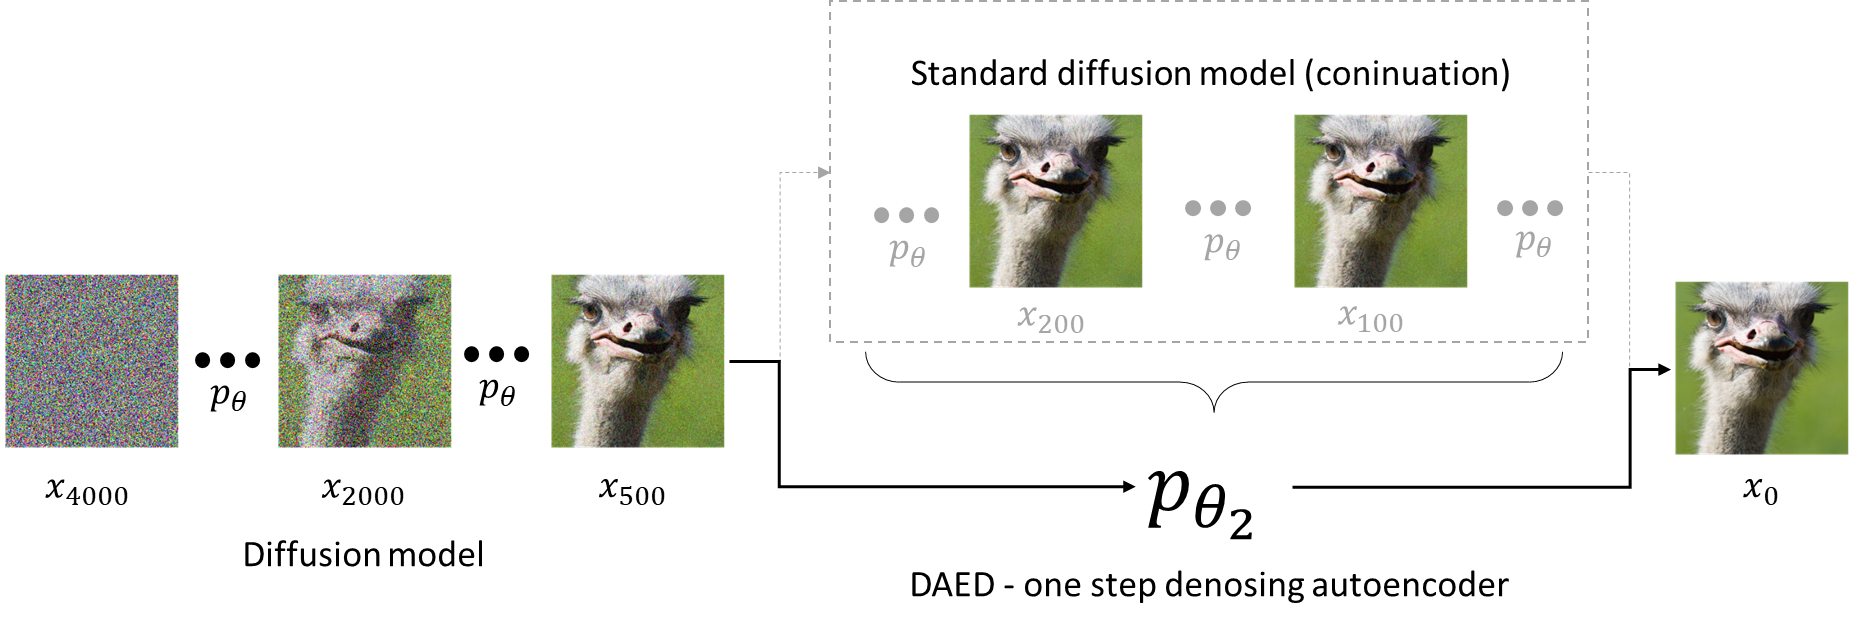
\includegraphics[width=.9\linewidth]{pics/4_daed/teaser.png}
    % \vskip  -4pt
	\caption{Overview of the proposed Denoising Auto-Encoder with Diffusion (DAED). To validate our hypothesis that DDGMs can be understood as a composition of a \emph{generator} and \emph{denoiser}, we propose to explicitly model the denoising part with a separate denoising autoencoder.}
	\label{fig:teaser}
% 	\vskip  -4pt
\end{figure}


In particular, we aim to answer the following three questions in this paper: 
\textbf{(i)} Is there a transition in the functionality of the backward diffusion process that switches from generating to denoising?
\textbf{(ii)} How does this split of functionality affect the performance? 
\textbf{(iii)} Does the denoising part in DDGMs generalize to other data distributions? 
As a result, the contribution of the paper is threefold:
\begin{itemize}
    \item First, we analyze the noise distribution in the forward diffusion process and how steps of the diffusion process are correlated with the reconstruction error.
    \item Second, based on our analysis, we postulate that DDGMs are composed of two parts: a \textit{denoiser} and a \textit{generator}. As a result, we propose a new class of models that consist of a Denoising Auto-Encoder and a Diffusion-based generator shortened as DAED. \ours{} could be considered as a variation of DDGMs with an explicit split into the denoising part and the generating part. 
    \item Third, we empirically assess the performance of DDGMs and \ours{} on three datasets (FashionMNIST, CIFAR10, CelebA) in terms of data generation and transferability (i.e., how DDGMs behave on different data distribution).
\end{itemize}


% = SECTION =

\section{Background}\label{sec:background}

% = SubSECTION =
\subsection{Diffusion-Based Deep Generative Models (DDGMs)}\label{sec:background_ddgm}


\paragraph{Model formulation}
We follow the formulation of the Diffusion-based Deep Generative Models (DDGMs) as presented in \cite{ho2020denoising,sohl2015deep}. DDGMs could be seen as infinitely deep hierarchical VAEs with a specific family of variational posteriors \cite{huang2021variational, kingma2021variational, tomczak2022deep, tzen2019neural}, namely, Gaussian diffusion processes \cite{sohl2015deep}. Given a data point $\rvx_0$ and latent variables $\rvx_{t}, \ldots, \rvx_{T}$, we want to optimize the marginal likelihood $p_{\theta}(\rvx_0) = \int p_{\theta}(\rvx_0, \ldots, \rvx_{T}) \mathrm{d} \rvx_1, \ldots, \rvx_{T}$. We define the \textit{backward} (or \textit{reverse}) \textit{process} as a Markov chain with Gaussian transitions starting with $p(\rvx_T) = \mathcal{N}(\rvx_{T}; \boldsymbol{0}, \mathbf{I})$, that is:
\begin{equation} \label{eq:backward_diffusion}
    p_{\theta}(\rvx_0, \ldots, \rvx_{T}) = p(\rvx_T)\ \prod_{t=0}^{T} p_{\theta}(\rvx_{t-1} | \rvx_{t}),
\end{equation}
where $p_{\theta}(\rvx_{t-1} | \rvx_{t}) = \mathcal{N}(\rvx_{t-1}; \mu_{\theta}(\rvx_{t}, t), \Sigma_{\theta}(\rvx_{t}, t))$.
Additionally, we define the \textit{forward diffusion process} as a Markov chain that gradually adds Gaussian noise to the data according to a variance schedule $\beta_1,...,\beta_T$, namely, $q(\rvx_1, \ldots , \rvx_{T} | \rvx_{0}) = \prod_{t=1}^{T} q(\rvx_t | \rvx_{t-1})$, where $q(\rvx_t|\rvx_{t-1}) = \mathcal{N}(\rvx_t; \sqrt{1 - \beta_t} \rvx_{t-1}, \beta_t \mathbf{I})$. 
Let us further define $\alpha_t = 1 - \beta_t$ and $\overline{\alpha}_t = \prod_{i=0}^{t} \alpha_{i}$. Since the conditionals in the forward diffusion can be seen as Gaussian linear models, we can analytically calculate the following distributions: 
\begin{equation}\label{eq:forward_diffusion_latent_from_data}
    q(\rvx_t|\rvx_0) = \mathcal{N}(\rvx_t; \sqrt{\overline{\alpha}_t} \rvx_0, (1 - \overline{\alpha}_t) \mathbf{I}),
\end{equation}
and 
\begin{equation}\label{eq:forward_diffusion_previous_latent}
q(\rvx_{t-1}|\rvx_{t}, \rvx_0) = \mathcal{N}(\rvx_{t-1}; \Tilde{\mu}(\rvx_t, \rvx_0), \Tilde{\beta}_t \mathbf{I}) ,
\end{equation}
where $\Tilde{\mu}(\rvx_t, \rvx_0) = \frac{\sqrt{\overline{\alpha}_{t-1}} \beta_{t}}{1-\overline{\alpha}_{t}} \rvx_0 + \frac{\sqrt{\alpha_{t}}\left(1-\overline{\alpha}_{t-1}\right)}{1-\overline{\alpha}_{t}} \rvx_{t}$, 
and $\Tilde{\beta}_{t}=\frac{1-\overline{\alpha}_{t-1}}{1-\overline{\alpha}_{t}} \beta_{t}$. We can use (\ref{eq:forward_diffusion_latent_from_data}) and (\ref{eq:forward_diffusion_previous_latent}) to define the variational lower bound as follows:
\begin{align} \label{eq:diff_elbo}
    \ln p_{\theta}(\rvx_0) \geq L_{vlb}(\theta) := &\underbrace{\E_{q(\rvx_1|\rvx_0)}[\ln p_{\theta}(\rvx_0|\rvx_1)]}_{-L_0} - \underbrace{\KL{q(\rvx_T |\rvx_0)}{p(\rvx_T)}}_{L_T} \notag \\
    & - \sum_{t=2}^T \underbrace{\E_{q(\rvx_t|\rvx_0)} \KL{q(\rvx_{t-1}|\rvx_t, \rvx_0)}{p_{\theta}(\rvx_{t-1}|\rvx_t)}}_{L_{t-1}}.
\end{align}
that we further optimize with respect to the parameters of the backward diffusion.

\paragraph{The conditional likelihood} 
In this paper, we focus on images, thus, data is represented by integers from $0$ to $255$. Following \cite{ho2020denoising}, we scale them linearly to $[-1, 1]$. As a result, to obtain discrete log-likelihoods, we consider the discretized (binned) Gaussian conditional likelihood \cite{ho2020denoising}:
\begin{equation}\label{eq:discretized_Gaussian}
    p_{\theta}\left(\rvx_{0} | \rvx_{1}\right)=\prod_{i=1}^{D} \int_{\delta_{-}\left(x_{0}^{i}\right)}^{\delta_{+}\left(x_{0}^{i}\right)} \mathcal{N}\left(x ; \mu_{\theta}^{i}\left(\mathbf{x}_{1}, 1\right), \sigma_{1}^{2}\right) \mathrm{d} x, 
\end{equation}
where $D$ is the data dimensionality of $\rvx_0$, and $i$ denotes one coordinate of $\rvx_0$, and:
\begin{equation}
    \delta_{+}(x)=\left\{\begin{array}{ll}
\infty & \text { if } x=1 \\
x+\frac{1}{255} & \text { if } x<1
\end{array} \quad \delta_{-}(x)= \begin{cases}-\infty & \text { if } x=-1 \\
x-\frac{1}{255} & \text { if } x>-1\end{cases}\right. .
\end{equation}

\paragraph{Noise scheduling} Originally, \cite{ho2020denoising} propose to linearly scale the noise parameters $\beta_t$ (\textit{linear scheduling}), e.g., scaling linearly from $\beta_1 = 10^{-4}$ to $\beta_{T} = 0.02$. In   \cite{nichol2021improved}, authors suggest to increase the number of less noisy steps through \textit{cosine scheduling}: % (\textit{cosine scheduling}, 
$\bar{\alpha}_{t}=\frac{f(t)}{f(0)}$, $f(t)=\cos \left(\frac{t / T+c}{1+c} \cdot \frac{\pi}{2}\right)^{2}, c > 0$
with clipping the values of $\beta_t$ to $0.999$ to prevent potential instabilities at the end of the diffusion.

\paragraph{Training details} In \cite{ho2020denoising}, authors notice that a single part of the variational lower bound is equal to:
\begin{equation}\label{eq:l_t}
    L_{t}(\theta) = \mathbb{E}_{\rvx_{0}, \boldsymbol{\epsilon}}\left[\frac{\beta_{t}^{2}}{2 \sigma_{t}^{2} \alpha_{t}\left(1-\overline{\alpha}_{t}\right)}\left\|\boldsymbol{\epsilon}-\boldsymbol{\epsilon}_{\theta}\left(\sqrt{\overline{\alpha}_{t}} \rvx_{0}+\sqrt{1-\overline{\alpha}_{t}} \boldsymbol{\epsilon}, t\right)\right\|^{2}\right] ,
\end{equation}
where $\boldsymbol{\epsilon} \sim \mathcal{N}(\mathbf{0}, \mathbf{I})$ and $\boldsymbol{\epsilon}_\theta$ is a neural network predicting the noise $\boldsymbol{\epsilon}$ from $\rvx_t$.
Since we use (\ref{eq:forward_diffusion_previous_latent}) in the variational lower bound objective (\ref{eq:diff_elbo}), and $\rvx_t$ could be sampled from the forward diffusion for a given data, see (\ref{eq:forward_diffusion_latent_from_data}), we can optimize one layer at a time. In other words, we can randomly pick a specific component of the objective, $L_t$, and update the parameters by optimizing $L_t$ without running the whole forward process from $\rvx_0$ to $\rvx_T$. As a result, the training becomes very efficient and learning very deep models (with hundreds or even thousands of steps) is possible.

In \cite{ho2020denoising}, it is also proposed to train a simplified objective that is a version of (\ref{eq:l_t}) without scaling, namely:
\begin{equation}\label{eq:l_t_simple}
    L_{t,\text {simple}}(\theta) = \mathbb{E}_{\mathbf{x}_{0}, \boldsymbol{\epsilon}}\left[\left\|\boldsymbol{\epsilon}-\boldsymbol{\epsilon}_{\theta}\left(\sqrt{\overline{\alpha}_{t}} \mathbf{x}_{0}+\sqrt{1-\overline{\alpha}_{t}} \boldsymbol{\epsilon}, t\right)\right\|^{2}\right] ,
\end{equation}
where $t$ is uniformly sampled between $1$ and $T$. To further reduce computational and memory costs, typically, a single, shared neural network is used for modeling $\boldsymbol{\epsilon}_{\theta}$ \cite{ho2020denoising, kingma2021variational, nichol2021improved} that is parameterized by an architecture based on U-Net type neural net \cite{ronneberger2015u}. The U-Net could be seen as a specific auto-encoder that passes all codes from the encoder to the decoder.

% = SubSECTION =
\subsection{Denoising Auto-Encoders}
Another class of models, Denoising Auto-Encoders (DAEs), is similar to DDGMs in the sense that they also revert a known corruption process. However, DAEs are trained to remove the noise in a single pass, and unlike DDGMs, they cannot generate new objects. Specifically, DAEs are auto-encoders that reconstruct a data point $\rvx_0$ from its corrupted (noisy) version \cite{alain2014regularized, bengio2013generalized, chen2014marginalized, vincent2008extracting}. Let us denote the auto-encoder by $f_{\varphi}(\cdot)$. Using the same notation as for DDGMs, the Gaussian corruption distribution is $q(\rvx_1 | \rvx_0)$. Then, a DAE maximizes the following objective function:
\begin{equation}
    \ell(\rvx_0;\varphi) = \mathbb{E}_{q(\rvx_1 | \rvx_0)}\left[\ln p\left(\rvx_0 | f_{\varphi}\left(\rvx_1\right)\right)\right] .
\end{equation}
and, in particular, for the Gaussian distribution with the identity covariance matrix, we get the original objective for DAEs \cite{vincent2008extracting}: $\ln p\left(\rvx_0 | f_{\varphi}\left(\rvx_1\right)\right) = -\left\| \rvx_0 - f_{\varphi}\left(\rvx_1\right) \right\|^2 + const$.


% = SECTION =

% = SECTION =
\section{An analysis of DDGMs \label{sec:analysis}}

The core idea behind DDGMs is the gradual noise injection to images as we go forward in time such that the final object is a sample from the standard Gaussian distribution. Then, in the backward diffusion process model reverts this procedure and, as a result, generates new objects. Therefore, understanding the success of DDGMs relies heavily on understanding how the injected noise influences the behavior of both training and the model itself.

\paragraph{The noise distribution in the forward diffusion process} The first question we ask is how much corrupted an image gets after applying a specific noise schedule. Following %other work (e.g., 
\cite{ho2020denoising, kingma2014autoencoding, nichol2021improved}, we can utilize the signal-to-noise ratio (SNR), expressed as the squared mean of a signal (here: image) divided by the variance of a signal, to quantify the amount of noise in $\rvx_t$. For this purpose, the quantity of interest is the forward diffusion for a given $\rvx_0$, namely, $q(\rvx_t | \rvx_0)$, that results in the following SNR:
\begin{equation}\label{eq:snr}
    SNR(\rvx_0, t) = \frac{\overline{\alpha}_t \rvx_0^2}{1 - \overline{\alpha}_t} .
\end{equation}

Similarly to \cite{kingma2021variational}, we formulate the forward diffusion in such a way that the SNR is strictly monotonically decreasing in time, namely, $SNR(\rvx_0, t) < SNR(\rvx_0, s)$ for $t > s$. This means that an image becomes more noisy as we go forward in time. 

\begin{figure}[h!]
	\centering
    \subfloat[Linear noise schedule]{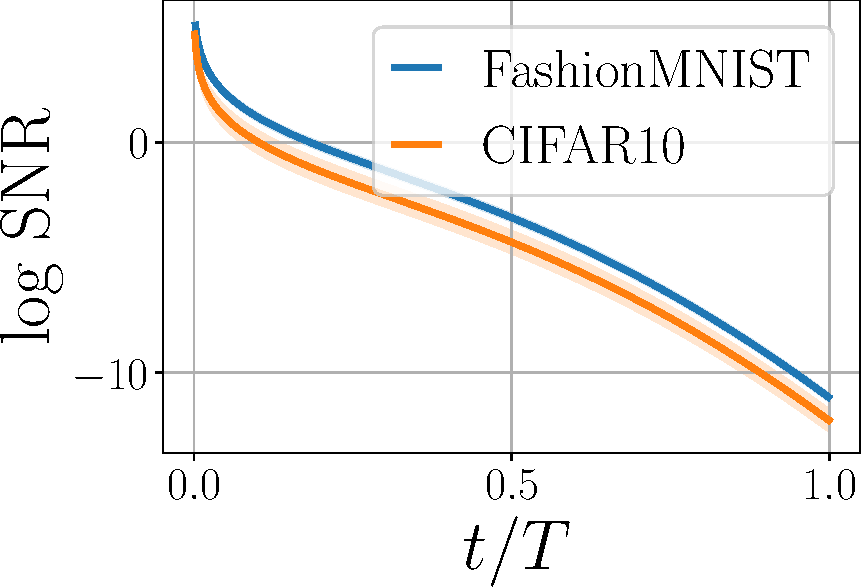
\includegraphics[width=0.34\linewidth]{pics/4_daed/snr/linear_0_1.0_snr_w.pdf}
    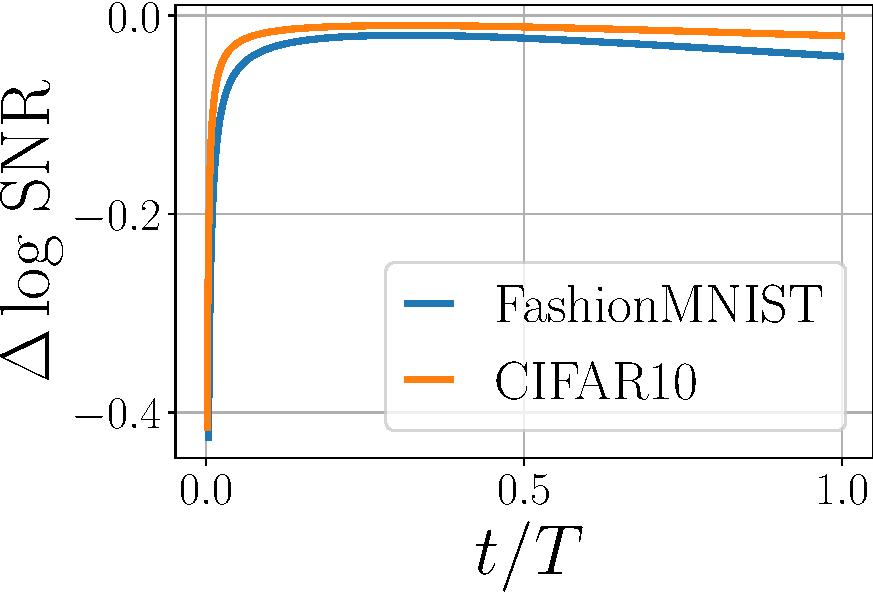
\includegraphics[width=0.34\linewidth]{pics/4_daed/snr/linear_0_1.0_delta_snr.pdf}}  \quad
    \subfloat[Cosine noise schedule]{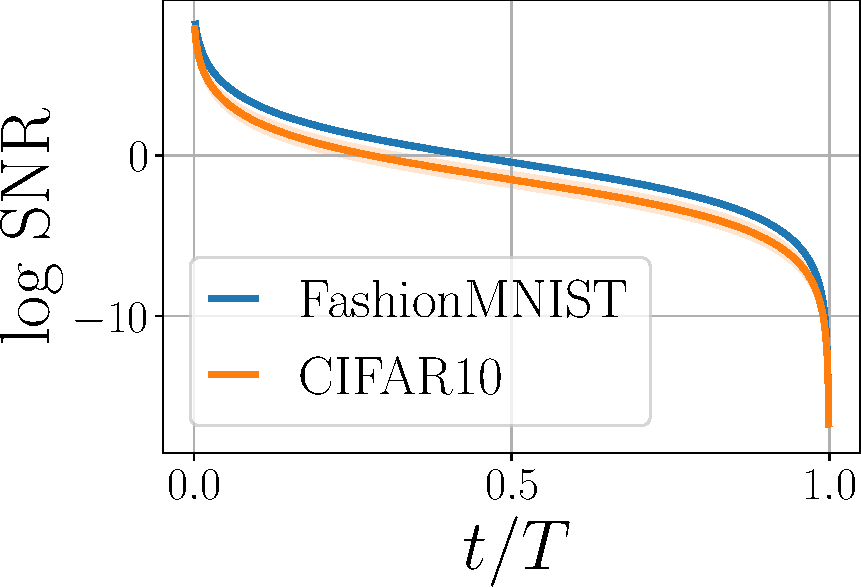
\includegraphics[width=0.34\linewidth]{pics/4_daed/snr/cosine_0_1.0_snr_w.pdf} 
    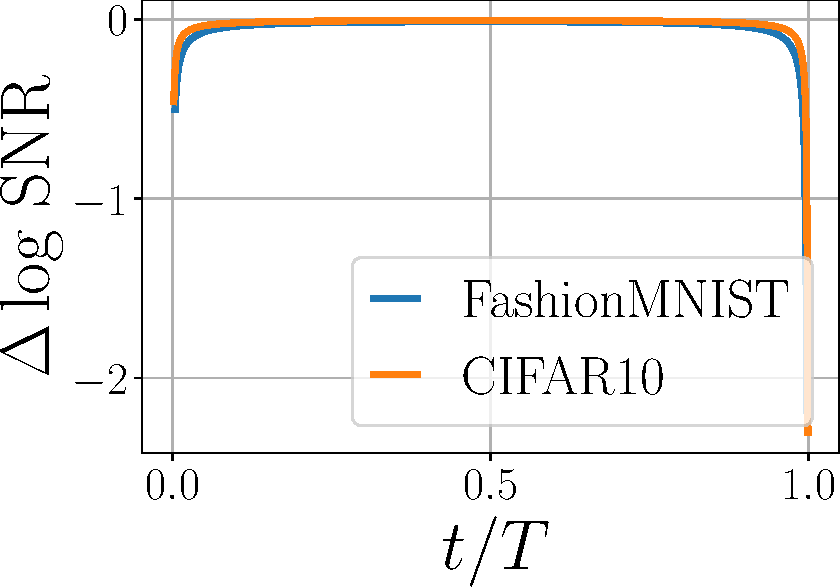
\includegraphics[width=0.34\linewidth]{pics/4_daed/snr/cosine_0_1.0_delta_snr.pdf}}
    % \vskip  -4pt
	\caption{Logarithm of the signal-to-noise ratio averaged over the dataset (solid line) and its standard deviation, and the difference of the $\log$ SNR within two consecutive time steps.}
	\label{fig:snr_analysis}
	\vskip  -4pt
\end{figure}

In Figure \ref{fig:snr_analysis} (left) we plot the logarithm of the SNR for both linear (Figure \ref{fig:snr_analysis}.a) and cosine (Figure \ref{fig:snr_analysis}.b) noise schedules for two datasets (FashionMNIST and CIFAR10). We average SNR over the $\rvx_0$'s (from the corresponding dataset). The right column depicts the change of the $\log$ SNR, i.e., its discrete derivative $\Delta \log \text{SNR}(t) = \log \text{SNR}(x_0, t) - \log \text{SNR}(x_0, t-1)$. First of all, we can notice a point at which the log-SNR drops below $0$. This corresponds to the situation of the noise overshadowing the signal. In the case of the linear noise schedule, this happens after about $20\%$ of steps, while for the cosine noise schedule, it appears after about $25-50\%$ of steps. However, the transition occurs in both cases. The biggest changes in the log-SNR are noticeable within the first $10\%$ of steps. This may suggest that the signal is the strongest within the first $10-20\%$ of the forward diffusion process steps, and then it starts being overshadowed by the noise. 

\paragraph{The reconstruction error of DDGMs} Since we know that the signal is not lost within the first $10-20\%$ of steps, the next question is about the reconstruction capabilities of DDGMs, namely, what is the reconstruction error of $\rvx_t \sim q(\rvx_t | \rvx_0)$. To be clear, we are not interested in how much each step of a DDGM contributes to the final objective (e.g., see Figure 2 in \cite{nichol2021improved}) but rather how well a DDGM reconstructs a noisy image $\rvx_t$.
In Figure \ref{fig:reconstruction_error_analysis} we plot the \textit{Mean Absolute Error} (MAE) and the \textit{Multi-Scale Structural Similarity} (MS-SSIM) \cite{wang2003multiscale} that both measure the difference between an original image $\rvx_0$ and a corrupted image at the $t^{th}$ step $\rvx_t$ reversed by the backward diffusion. 

%\begin{wrapfigure}{r}{0.57\textwidth}
%% \vskip  -11pt
%    \begin{adjustbox}{center}
     \begin{figure}[t]
    \begin{tabular}{cc}
    %   $\log$ SNR $(t)$ &  $\Delta$ $\log$ SNR $(t)$ \\
        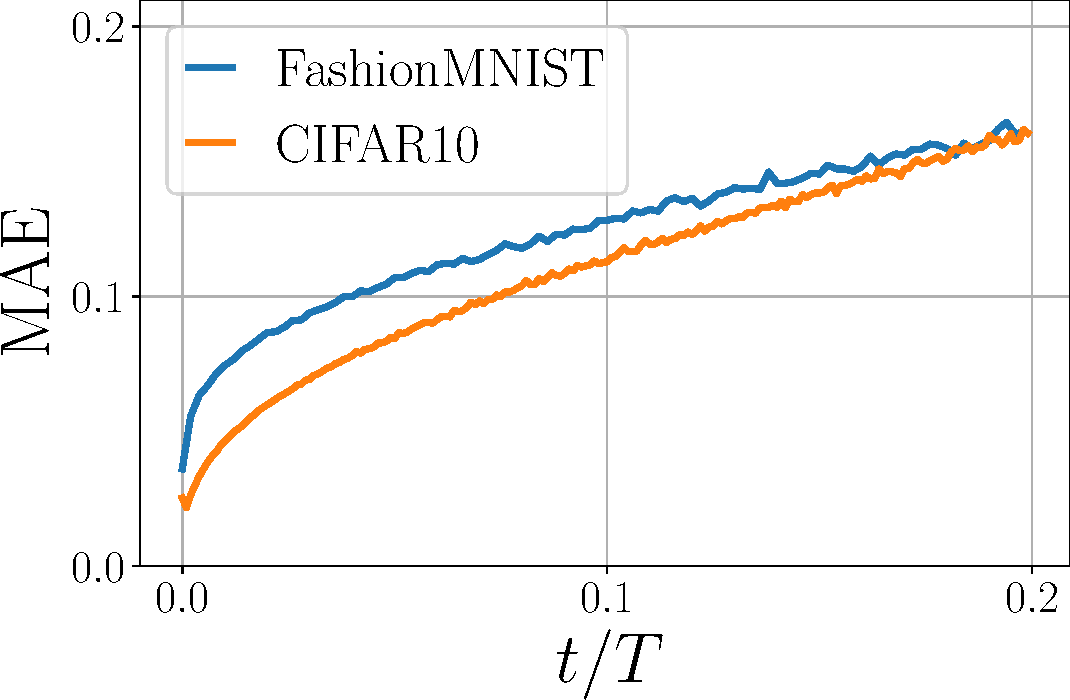
\includegraphics[width=0.4\textwidth]{pics/4_daed/experiments/MAE_step.pdf} &
        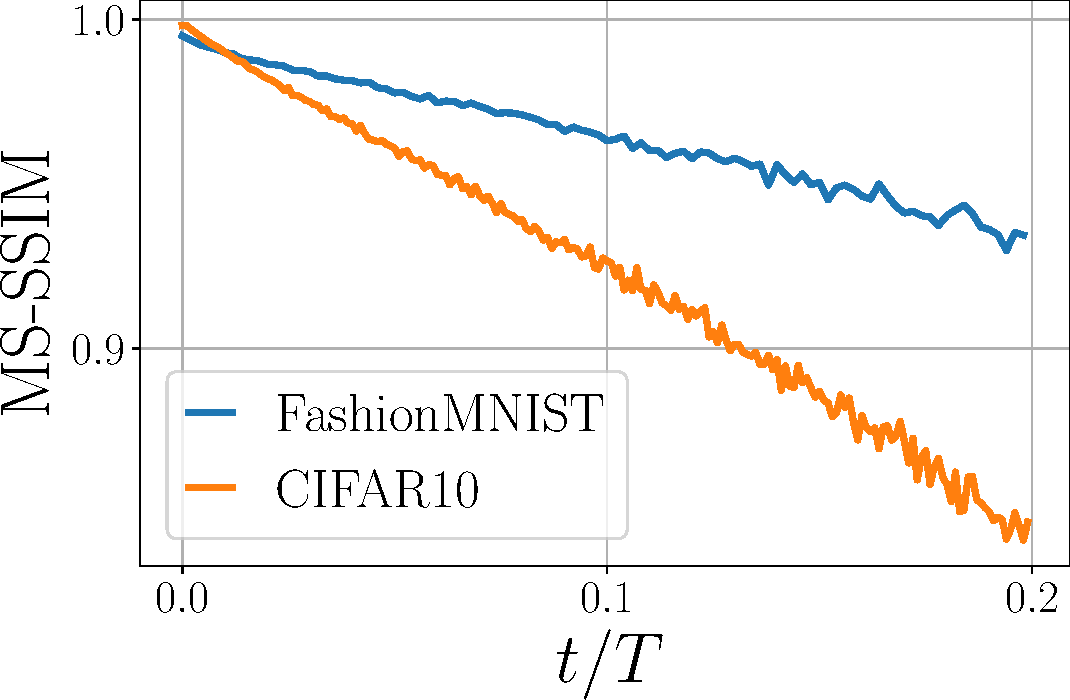
\includegraphics[width=0.4\textwidth]{pics/4_daed/experiments/MSSSIM_step.pdf} \\
    \end{tabular}
%    \end{adjustbox}
    \caption{The averaged reconstruction error calculated using (\textit{left}) the MAE, and (\textit{right}) the MS-SSIM at different steps of a DDGM.}
    \label{fig:reconstruction_error_analysis}
    \vspace*{\baselineskip}
     \end{figure}
%\end{wrapfigure}


We present the values on two datasets (FashionMNIST and CIFAR10) for the first 20\% of steps. Apparently, after around $10\%$ of the steps, the reconstruction error starts growing, and the MAE increases linearly above $0.1$ (i.e., about $6\%$ of error per pixel). At the same time, the MS-SSIM drops below $0.9-0.95$ (i.e., the discrepancy between original images and reconstructions becomes perceptually evident). This observation might suggest that DDGMs could be roughly divided into two parts: a fraction of steps of a DDGM (e.g., first $10\%$ of the steps) constitute a \textit{denoiser} that turns a corrupted image into a clear image, and the remaining steps of the DDGM are responsible for turning noise into a noisy structure (a corrupted image), i.e., a \textit{generator} that generates meaningful patterns. In other words, we claim that DDGM can be interpreted as a composition of a denoiser and a generator, but the boundary between those two parts is fluid. Moreover, the denoiser gradually removes the noise in a generative manner (i.e., by sampling $\rvx_{t-1} \sim p(\rvx_{t-1}|\rvx_t)$).


\paragraph{DDGMs as hierarchical VAEs} In this paper, we postulate that DDGMs could be seen as a composition of parts that serve different purposes. We can get additional insight into our claim by noticing a close connection between DDGMs and hierarchical VAEs. As presented in \cite{huang2021variational,kingma2021variational,tomczak2022deep}, if we treat all $\rvx_t$'s with $t>0$ as latents, and see the forward diffusion process as a composition of (non-trainable) variational posteriors, DGGMs become a specific formulation of hierarchical VAEs. On the other hand, we can start with a VAE with a single latent variable, $\rvx_1$, for which the variational lower bound is equal to:
\begin{equation}
    \ln p(\rvx_0) \geq \mathbb{E}_{\rvx_1 \sim q(\rvx_1 | \rvx_0)}\left[\ln p(\rvx_0|\rvx_1)\right] - D_{\text{KL}}[q(\rvx_1 | \rvx_0)||p(\rvx_1)].
\end{equation}
Then, similarly to \cite{vahdat2021score,wehenkel2021diffusion}, the marginal $p(\rvx_1)$ could be further modeled by a DDGM. By keeping the dimensionality of $\rvx_1$ the same as $\rvx_0$, and taking the variational posterior $q(\rvx_1 | \rvx_0)$ to be fixed and part of the forward diffusion, we get the DDGM model. This perspective of combining a VAE with a DDGM opens new possibilities for developing hybrid models.

\section{\ours{}: Denoising Auto-Encoder with Diffusion}

In this work, we propose a specific combination that distinctly splits the DDGM into generative and denoising parts. As noted in the previous section, the signal in the forward diffusion process is the strongest within the first $10-20\%$ of steps, and, thus, we postulate to perceive this first part of a DDGM as a denoiser. 
Together with the observation about the combination of a VAE with a DDGM-based prior, we consider turning a denoising auto-encoder into a generative model as presented in Figure~\ref{fig:teaser}. We bring a DDGM-based part into DAE for generating corrupted images. The resulting objective is the following:
\begin{align}
    \overline{\ell}(\rvx_0;\varphi, \theta) &= \mathbb{E}_{\rvx_1 \sim q(\rvx_1 | \rvx_0)}\left[\ln p\left(\rvx_0 | f_{\varphi}\left(\rvx_1\right)\right) + \ln p_{\theta}(\rvx_1)\right] \label{eq:daed_1}\\ 
    &\geq \underbrace{\mathbb{E}_{\rvx_1 \sim q(\rvx_1 | \rvx_0)}\left[\ln p\left(\rvx_0 | f_{\varphi}\left(\rvx_1\right)\right)\right]}_{\ell_{\text{DAE}}(\rvx_0;\varphi)} \\
    &\quad + \underbrace{\mathbb{E}_{q(\rvx_2, \ldots , \rvx_T | \rvx_1)} \left[ \frac{\ln p_{\theta}(\rvx_1, \ldots, \rvx_T)}{q(\rvx_1, \ldots , \rvx_T | \rvx_0)} \right]}_{\ell_{\text{D}}(\rvx_0;\theta)} \label{eq:dead_2},
\end{align}
where in (\ref{eq:dead_2}) we introduce additional latent variables and the variational posterior over them, that yields the variational lower bound. We call the resulting model \textit{DAE with a Diffusion}, or DEAD for short. In a sense, DAED is a DDGM with distinct parameterizations of the part between $\rvx_0$ and $\rvx_1$, and the part for the remaining $\rvx$'s. Thus, DEAD is almost identical to a DDGM, but there are the following differences:
% \begin{itemize}[leftmargin=*]
%     \item We can control the amount of noise in $q(\rvx_1|\rvx_0)$. It can correspond to the first step of the forward diffusion model, or we can introduce more noise at once that would correspond to several steps in the DDGM.
%     \item We use two different parameterizations, namely, an auto-encoder (e.g., a U-Net architecture) for $f_{\varphi}(\cdot)$ and a separate, shared U-Net for modeling the DDGM from $\rvx_1$ to $\rvx_T$. Since there are two neural networks, the lower bound to the objective $\overline{\ell}$ is in fact a composition of two objectives with disjunctive parameters, namely, the objective for the \textit{denoiser}, $\ell_{\text{DAE}}$, and the objective for the \textit{generator} (i.e., the diffusion-based generative model), $\ell_{\text{D}}$.
%     \item In the \ours{}, we introduce the \textit{denoiser} explicitly and make a clear distinction between the denoising and the generating parts while, as discussed earlier, this boundary is rather fluid in DDGMs. By introducing \ours{}, we can analyze what happens if we distinctly divide those two aspects with two separate parametrizations.
% \end{itemize}
\textbf{(i)} We can control the amount of noise in $q(\rvx_1|\rvx_0)$. It can correspond to the first step of the forward diffusion model, or we can introduce more noise at once that would correspond to several steps in the DDGM. \textbf{(ii)} We use two different parameterizations, namely, an auto-encoder (e.g., a U-Net architecture) for $f_{\varphi}(\cdot)$ and a separate, shared U-Net for modeling the DDGM from $\rvx_1$ to $\rvx_T$. Since there are two neural networks, the lower bound to the objective $\overline{\ell}$ is in fact a composition of two objectives with disjunctive parameters, namely, the objective for the \textit{denoiser}, $\ell_{\text{DAE}}$, and the objective for the \textit{generator} (i.e., the diffusion-based generative model), $\ell_{\text{D}}$. \textbf{(iii)} In the \ours{}, we introduce the \textit{denoiser} explicitly and make a clear distinction between the denoising and the generating parts while, as discussed earlier, this boundary is rather fluid in DDGMs. By introducing \ours{}, we can analyze what happens if we distinctly divide those two aspects with two separate parametrizations.

Moreover, we hypothesize that the resulting model may better generalize across various data distributions due to decoupling the parameterization of the denoiser and the generator. The training dataset may bias a single, shared parameterization in a DDGM, and while denoising an image from a different domain, it may add some artifacts from the source. While with two distinct parameterizations, there might be a lower chance for that. We evaluate this hypothesis in the experiments. 

% = SECTION =
\section{Related work}

\textbf{DDGM for image generation} 
Various modifications of DDGMs were recently proposed to improve their sampling quality. This includes simplifying the learning objective and proposing new noise schedulers, which allow DDGMs to achieve state-of-the-art results. In this work, we show that splitting the decoder into two parts, namely, a denoiser and a generator, can benefit the performance, especially when training with the variational lower bound.

\textbf{Properties of DDGMs} 
In~\cite{ho2020denoising} authors notice that DDGMs can be beneficial for lossy compression, observing (Figure 5 in~\cite{ho2020denoising}) that most of the bits are allocated to the region of the smallest distortion that corresponds to the first steps of a DDGM. 
We draw a similar conclusion when discussing the denoising ability of the diffusion model in Section \ref{sec:analysis}. However, we base our analysis on the signal-to-noise ratio rather than compression. On the other hand~\cite{salimans2022progressive} focus on the computational complexity of DDGM and propose a progressive distillation that iteratively reduces the number of diffusion steps. The work shows that it is possible to considerably reduce the number of sampling steps without losing performance. We believe that their results support our intuition that it is reasonable to combine several initial steps into a single denoiser model. In~\cite{benny2022dynamic}, authors evaluate how the diffusion process changes in time when model is trained with different objectives (Eq.~\ref{eq:l_t} or Eq.~\ref{eq:l_t_simple}). They observe that the image generation process differs significantly and that it is more beneficial to switch between those two approaches at different stages of the diffusion. 
In this work, we also investigate changes in the diffusion process, but we focus on the generative and denoising capabilities of the model instead.

\textbf{Connection to hierarchical Variational Autoencoders} Several works have noted the connection of DDGM to VAEs. In~\cite{huang2021variational} authors focus on the continuous diffusion models and draw the connection to the infinitely deep hierarchical VAEs. In~\cite{kingma2021variational} authors further explore this connection, formulate a VLB objective in terms of the signal-to-noise ratio and propose to learn noise schedule, which brings the forward diffusion process even closer to the encoder of a VAE. 
Recently a latent score-based generative model (LSGM) was proposed~\cite{vahdat2021score}, which can be seen as a VAE with the score-based prior. We follow a similar direction and propose to see a DDGM as a combination of a denoising auto-encoder with an additional diffusion-based generator of corrupted images.


% = SECTION =
\section{Experiments}


\paragraph{Experimental setup} In all the experiments, we use a U-Net-based architecture with timestep embeddings as proposed in~\citet{ho2020denoising,nichol2021improved}. We train all the models with a linear $\beta$ scheduler and uniform steps sampler to simplify the comparison. All implementation details and hyperparameters are included in the Appendix~\ref{appx:hyperparams} and code repository~\footnote{\url{https://github.com/KamilDeja/analysing_ddgm}}. 
For \ours{}, we use the same architecture for both the diffusion part and the denoising autoencoder. 
We run experiments on three standard benchmarks with different complexity: FashionMNIST~\cite{xiao2017fashion} of gray-scale $28 \times 28$ images, CIFAR-10~\cite{Krizhevsky09learningmultiple} of $32 \times 32$ natural images, and CelebA~\cite{liu2015faceattributes} of $64 \times 64$ photographs of faces. We do not use any augmentations during training for any dataset. We report results for both variational lower bound loss (VLB)~\cite{sohl2015deep} and simplified objective~\cite{ho2020denoising}.
Following~\citet{nichol2021improved} we evaluate the quality of generations with Fréchet Inception Distance (FID)~\cite{heusel2017gans} and distributions Precision (Prec) and Recall (Rec) metrics~\cite{sajjadi2018assessing} that disentangle FID score into two aspects: the quality of generated results (Precision) and their diversity (Recall).

\subsection{Is there a transition in functionality of the backward diffusion process that switches from generating to denoising?}
\label{sect:reasonable_to_use_denoiser}


In Section \ref{sec:analysis}, we investigate how the signal-to-noise ratio and the reconstruction error of a DDGM change with the increasing number of diffusion steps (see Figure \ref{fig:mae_cifar_celeba}). Based on this analysis, we postulate that DDGMs can be divided into two parts: a \emph{denoiser} and a \emph{generator}. To determine the switching point, we propose an experiment that answers the following question: \\
%\begin{wrapfigure}{r}{0.46\textwidth}
%\vskip  -12pt
%    \begin{adjustbox}{center}
%    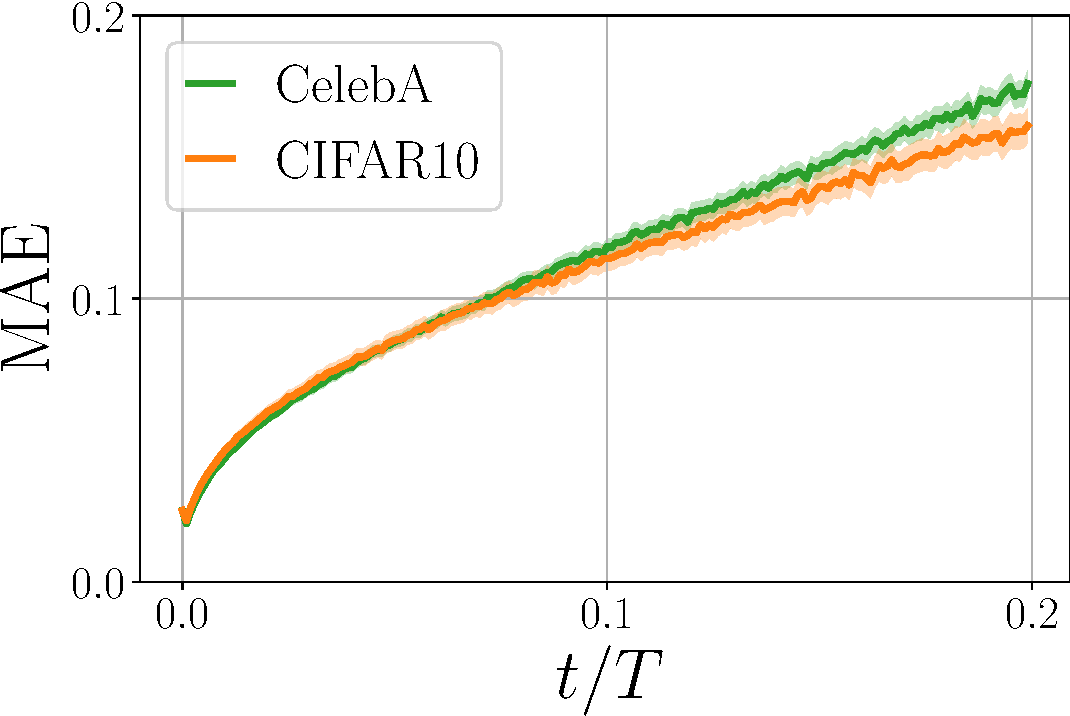
\includegraphics[width=0.4\textwidth]{pics/4_daed/experiments/MAE_step_cifar_celeba.pdf}
%    \end{adjustbox}
%    \vskip -6pt
%    \caption{The MAE for a DDGM trained on CIFAR10 and evaluated on CIFAR10 \& CelebA, with a 0.95 confidence interval.}
%    \label{fig:mae_cifar_celeba}
%    \vskip  -20pt
%    % \end{figure}
%\end{wrapfigure}
\textit{Is there a denoising part of a DDGM that is agnostic to the signal from the data?}
\begin{marginfigure}
	\vspace*{2\baselineskip}
	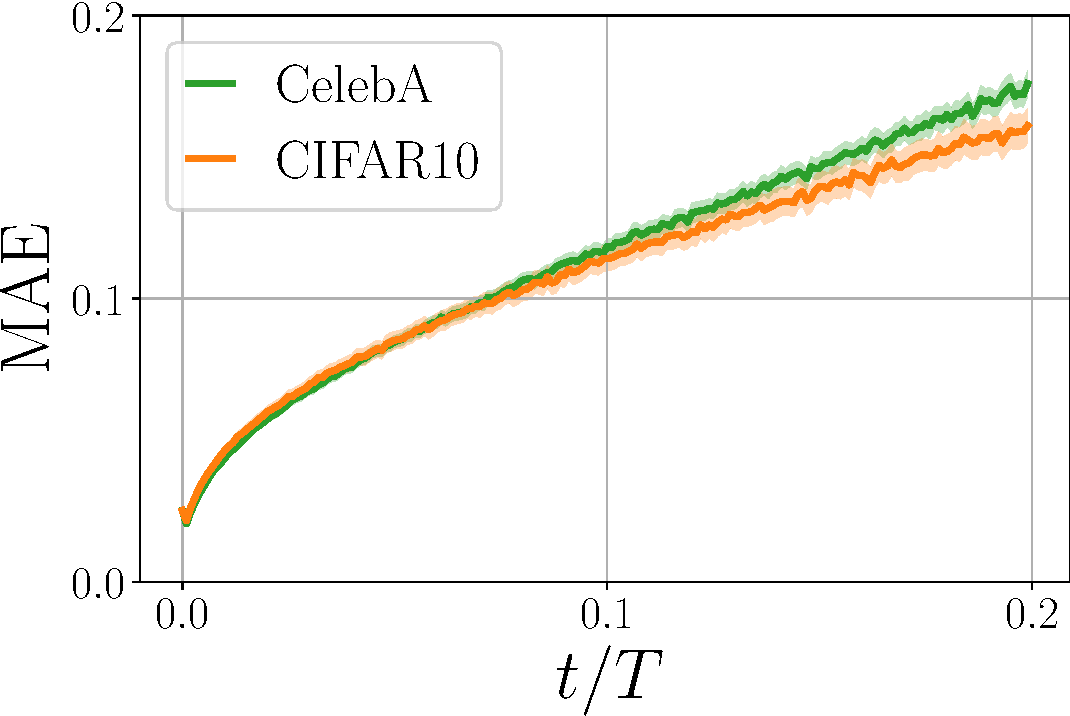
\includegraphics[width=\linewidth]{pics/4_daed/experiments/MAE_step_cifar_celeba.pdf}
	\caption{The MAE for a DDGM trained on CIFAR10 and evaluated on CIFAR10 \& CelebA, with a 0.95 confidence interval.}
	\label{fig:mae_cifar_celeba}
\end{marginfigure}
To that end, we refer once more to the analysis of the reconstruction error (e.g., MAE) from different diffusion steps. This time, however, we compare the quality of reconstructions with a single DDGM model trained on the CIFAR10 dataset and then evaluated on CIFAR10 and CelebA. The result of this experiment is presented in Figure \ref{fig:mae_cifar_celeba}. Interestingly, we notice that for approximately $10\%$ of the initial steps of the DDGM, there is a negligible difference in the reconstruction error between these two datasets. This fact may suggest that, indeed, the model does not require any information about the background data signal in the first steps, and it is capable of denoising corrupted images. However, after this point (about $10\%$ of steps), the reconstruction error starts growing faster for the dataset the model was not trained on. This indicates that information about the domain becomes important and affects performance.


\subsection{How does splitting DDGMs into generative and denoising parts affect the performance?}

The results so far confirm our claims that DDGMs could be divided into denoising and generative parts. Independently of a dataset, there appears to be a transition point at which a DDGM stops generating a corrupted image from noise and starts denoising it in a generative manner. Here, we aim to verify whether it is possible to do a clear split into a denoising part and a generating part. For this purpose, we use the introduced \ours{} approach that consists of a DAE part (the denoiser) and a DDGM (the generator) parameterized by two distinct U-Nets. 

\begin{figure}[t]
    % \vskip -4pt
	\centering
	\begin{tabular}{ccc}
	    	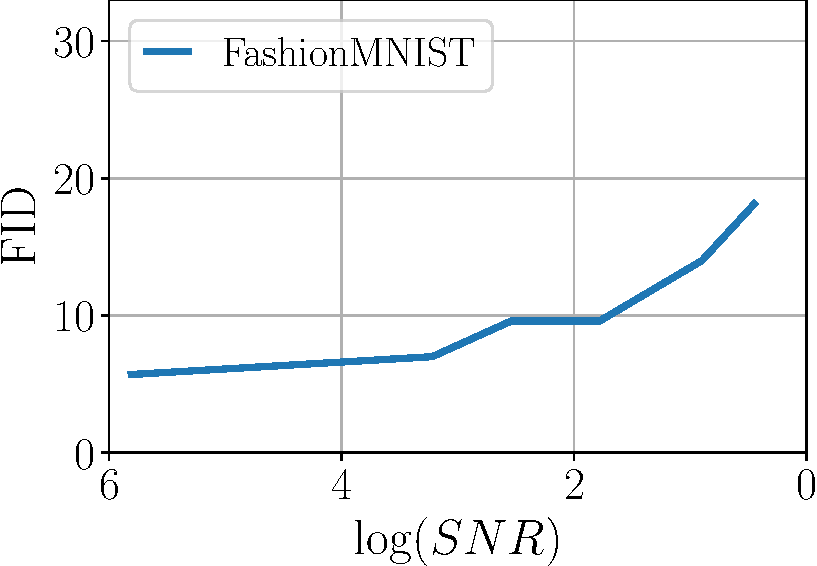
\includegraphics[width=0.3\linewidth]{pics/4_daed/experiments/fid_snr_fmnist.pdf} & %\label{fig:fid_snr_fmnist} &
	     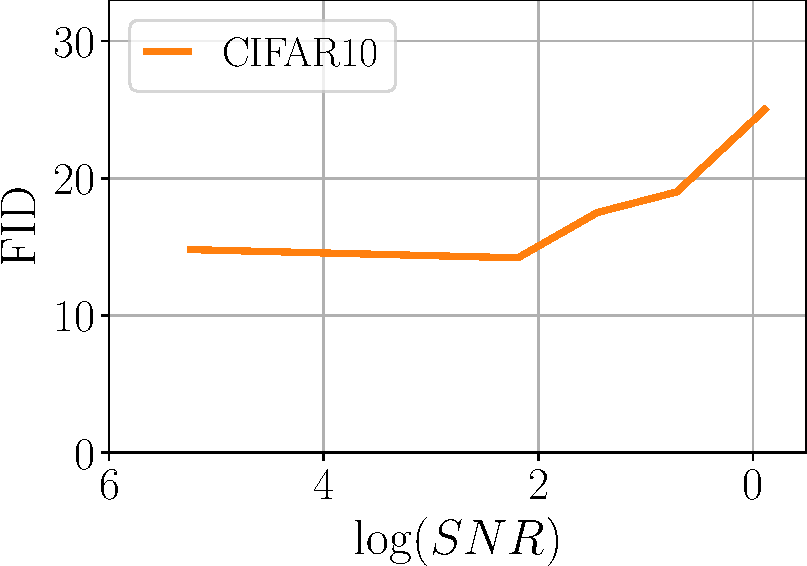
\includegraphics[width=0.3\linewidth]{pics/4_daed/experiments/fid_snr_cifar.pdf} & %\label{fig:fid_snr_cifar10}&
	      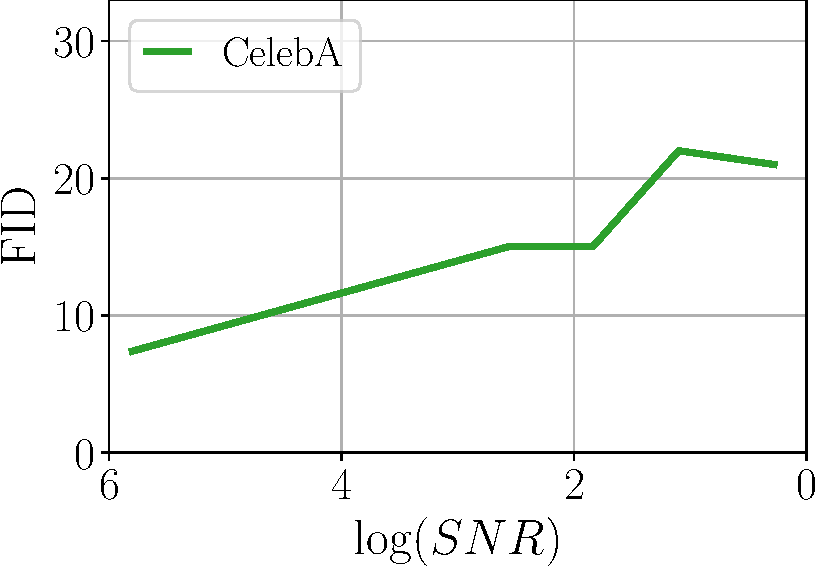
\includegraphics[width=0.3\linewidth]{pics/4_daed/experiments/fid_snr_celeba.pdf} \\ %\label{fig:fid_snr_celeba}\\
	    (a) FashionMNIST& (b) CIFAR10 & (c) CelebA 
	\end{tabular}
% 	\vskip -4pt
	\caption{ The performance (FID) of \ours{} with different switching points with respect to the logarithm of the signal to noise ratio (\protect\ref{eq:snr}) on three different datasets.}
	\label{fig:snr_fid}
	\vskip  -5pt
\end{figure}


First, we consider a situation in which we train a DDGM using the simplified objective (Eq.~\ref{eq:l_t_simple}) and then replace the first steps with a DAE. In other words, we train a \ours{} in two steps: first the DDGM and then the DAE. This experiment aims to check how the decoupling of the DDGM into two parts influences the model performance. In Figure~\ref{fig:snr_fid} we present the dependency between the log-SNR at the splitting point and the FID score. In all cases, the performance of \ours{} is comparable to the DDGM if we replace the DAE with up to the $10\%$ of the steps that correspond to $log(SNR)$ is equal to around $4$. For more complicated datasets like CIFAR10 and CelebA, fewer steps could be replaced. This effect could be explained by the fact that images in these datasets have three channels (RGB), and removing noise is more problematic. That outcome reconfirms our presumptions that it is reasonable to split the DDGM since the final performance is not significantly affected by the division for an adequately chosen splitting point.

% \begin{wrapfigure}{r}{0.6\textwidth}
% \vskip  -10pt
\begin{figure}
    \begin{adjustbox}{center}
    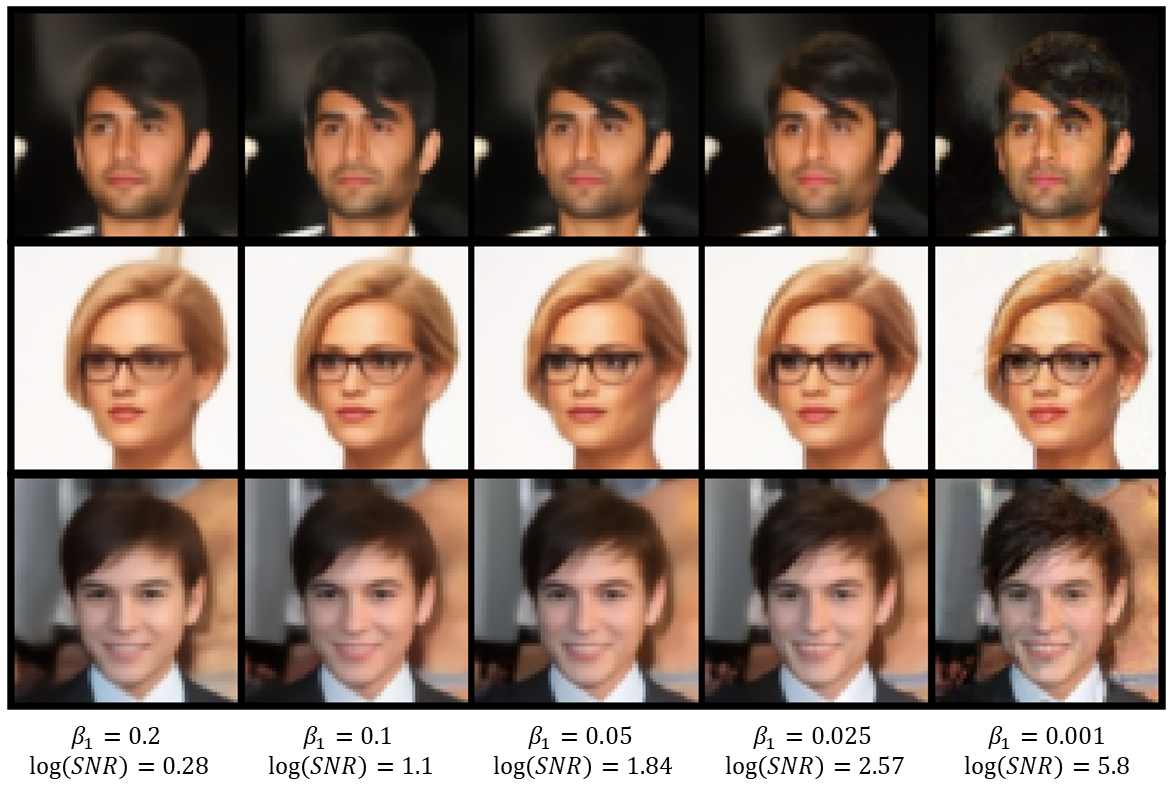
\includegraphics[width=0.8\linewidth]{pics/4_daed/experiments/daed_generations.png}
    \end{adjustbox}
    \caption{Examples of generations from \ours{} with the same noise value and different switching points.}
    \label{fig:daed_generations} 
% \vspace*{\baselineskip}
    \end{figure}
% \end{wrapfigure}

To get further insight into the qualitative performance, in Figure~\ref{fig:daed_generations} we demonstrate how the selection of the splitting point with respect to the Signal to Noise Ratio (SNR) affects the quality of final generations\footnote{Generations for all datasets are presented in Appendix~\ref{appx:generation}}. We present non-cherry-picked samples from \ours{} trained in the same manner as described in the previous paragraph. As expected, the more noise the DAE part (the denoiser) must deal with (see the values of $\beta_1$ in Figure~\ref{fig:daed_generations}), the fewer details in the generations there are. These samples again indicate that by replacing some steps with a denoiser, we get a trade-off between ''cleaning'' the corrupted image or, in fact, further generating details. It seems that there is a sweet spot for perceptually appealing images that contain details and are ''smooth'' at the same time, see $\beta_1=0.025$ in Figure~\ref{fig:daed_generations}. However, as it is typically difficult to provide convincing arguments by \textit{staring} at samples, we further propose to analyze quantitative measures.

\begin{table*}[t!]
  \centering
  \captionsetup{width=1.4\textwidth, margin={0pt, -.4\textwidth}}
  \caption{FID Precision (Prec) and Recall (Rec) scores. For each row, we indicate the length of the diffusion process (T) and the training objective (Loss). \textbf{Best results in bold}.}
  \label{tab:results_fmnist_cifar_celeba}
  \vskip -5pt
  \resizebox{1.4\textwidth}{!}{
  \begin{tabular}{l|c||c|ccc||c|ccc||c|ccc}
    \toprule
     \multicolumn{2}{c||}{Model} & \multicolumn{4}{c||}{Fashion Mnist} & \multicolumn{4}{c||}{CIFAR10} &   \multicolumn{4}{c}{CelebA} \\
    \midrule
    & Loss & T & FID $\downarrow$&Prec $\uparrow$ & Rec $\uparrow$ & T & FID $\downarrow$ & Prec $\uparrow$ & Rec $\uparrow$ & T & FID $\downarrow$ & Prec $\uparrow$ & Rec $\uparrow$\\

    \midrule
    DDGM & VLB & 500 & 8.9 & 68 & 53 & 1000 & 26 & 53 & 54 & 1000 & 23 & 51 &21\\
    \ours{} $\beta_1=0.1$ & VLB & 468 & 9.1 & \textbf{71} & 60 & 900 & 20 & 59 & 46 & 900 & 18 & 63 & \textbf{30}\\
    \ours{} $\beta_1=0.001$ & VLB & 499 & \textbf{7.5} & \textbf{71} & \textbf{64} & 999 & \textbf{15} & \textbf{60} & \textbf{60} & 999 & \textbf{16} & \textbf{70} & 27 \\
    \midrule
    DDGM & Simple & 500 & 7.8 & 72 & \textbf{65} & 1000 & \textbf{7.2} & \textbf{65} & \textbf{61} & 1000 & \textbf{4.9} & 66 & \textbf{57}\\
    \ours{} $\beta_1=0.1$& Simple & 468 & 9.6 & \textbf{73} & 58 & 900 & 19 & 62 & 50 & 900 & 22 & \textbf{67} & 27 \\
    \ours{} $\beta_1=0.001$ &Simple & 499 & \textbf{5.7} & 69 & 64 & 999 & 14.8 & \textbf{65} & 53 & 999 & 7.4 & \textbf{67} & 54 \\
    \bottomrule
  \end{tabular}}
% \vspace*{\baselineskip}
\end{table*}

In Table \ref{tab:results_fmnist_cifar_celeba}, we compare the performance of \ours{} against the DDGM on FashionMNIST, CIFAR10, and CelebA in terms of FID, Precision and Recall scores. We want to highlight that our goal is not to achieve SOTA results on the before-mentioned datasets but to verify whether we can gain some further understanding and, potentially, some improvement by splitting the denoising and generative parts. We consider two scenarios, namely, learning a DDGM and \ours{}s using either the variational lower bound (VBL) or the simplified objective (Simple) with various lengths of the diffusion. Interestingly, \ours{} outperforms the DDGM when these models are trained using the VBL loss. For the simplified objective, \ours{} trained with the same number of diffusion steps yields slightly lower performance than standard DDGMs. As indicated by the Precision/Recall, generations from \ours{} are as precise as those from DDGM. However, they lack certain diversity, probably due to the smoothing effect of the DAE part. Detailed results for other setups are presented in Appendix~\ref{appendix:extra_results}.\footnote{In Appendix~\ref{appx:large_models} we show that increasing the number of parameters of DDGMs to be comparable to \ours{} does not lead to significant performance improvements.}

\subsection{Does the noise removal in DDGMs generalize to other data distributions?}
The last question we are interested in is the generalizability of DDGMs to other data distributions. We refer to this concept as \textit{transferability} for short. In other words, the goal of this experiment is to determine whether we can reuse a model or its part on new data with as good performance as possible. In this experiment, we rely on the results presented in Section~\ref{sect:reasonable_to_use_denoiser} where roughly the first $10\%$ of steps could be seen as the denoising part. To further strengthen this perspective, we also utilize \ours{} with an explicit division into the denoising and generating parts.

\begin{table}[t]
  \centering
  \caption{Reconstruction errors measured by MAE~($\downarrow$), MS-SSIM~($\uparrow$) for images noised with $\beta_1=0.1$. \\
  	*To evaluate models trained on CIFAR10, we downscale CelebA to $32\times32$. \textbf{Best results in bold.}}
  \vskip -5pt
  \resizebox{\textwidth}{!}{
  \begin{tabular}{c|l||cccccc}
    \toprule
    & Target dataset & \multicolumn{2}{c}{CIFAR10} & \multicolumn{2}{c}{CIFAR100} & \multicolumn{2}{c}{CelebA*}\\
    \midrule
    Source Dataset& Model& MAE & MS-SSIM & MAE & MS-SSIM & MAE & MS-SSIM \\ 
    \midrule
    \multirow{3}{*}{CIFAR10} & DDGM VLB & 0.091 &0.94 & 0.097 &0.94 & 0.093 &0.95 \\
    & DDGM Simple & 0.085 & 0.95 & 0.097 & 0.94 & 0.096 & 0.95\\
    & \ours{} & \textbf{0.065} & \textbf{0.97} & \textbf{0.074} & \textbf{0.97} & \textbf{0.068} & \textbf{0.97}\\
    \midrule
    \multirow{3}{*}{ImageNet} & DDGM VLB & 0.113 & 0.93 & 0.110 & 0.93 & 0.077 & 0.96\\
    & DDGM Simple & 0.113 & 0.94 & 0.111 & 0.93 & 0.068 & 0.96\\
    & \ours{} & \textbf{0.071} & \textbf{0.97} & \textbf{0.071} & \textbf{0.97} & \textbf{0.050} & \textbf{0.98}\\
    \bottomrule
  \end{tabular}
  }
  \label{tab:transferability}
\end{table}

First, we consider the case in which we compare the reconstruction errors measured by the MAE and the MS-SSIM. In this scenario, we train a DDGM on a source dataset and then assess it on a target dataset. We use CIFAR10 or ImageNet (32x32 or 64x64) as source data and CIFAR10, CIFAR100, or CelebA as target data. For each image from the target dataset, we apply the DAE part of \ours{} to obtain the reconstruction or 793 steps of the forward and backward diffusion in the case of the DDGM, which corresponds to the same level of added noise. For this experiment, we use the pre-trained DDGM from \citet{nichol2021improved} that consists of 4000 steps and uses the cosine noise scheduler. The results are outlined in Table~\ref{tab:transferability}. First of all, there is no significant difference in the performance of DDGMs trained with either the VBL objective or the simplified objective. They achieve a quite satisfactory MAE and MS-SSIM scores. However, \ours{} outperforms the DDGMs, obtaining much better transferability. We explain it by the fact that probably, with each step in the denoising part DDGM adds details that are typical for source data while \ours{} focuses on removing noise and produces a smoother output. This outcome may further suggest that splitting DDGMs into two parts with two separate parameterizations is reasonable and even beneficial.

To get further insight into the transferability behavior, we present a few (non-cherry-picked) examples from CelebA in Figure~\ref{fig:transferability}a and four toy examples in Figure~\ref{fig:transferability}b. We use the same setup as explained in the previous paragraph (i.e., the pre-trained DDGM provided in \citet{nichol2021improved}), and the images are noised with $\beta_1=0.1$. In columns 3--6 in Figure~\ref{fig:transferability}a, we present reconstructions for the DDGM trained on CelebA, the DDGM trained on ImageNet, \ours{} trained on CelebA, and \ours{} trained on ImageNet, respectively. It becomes apparent that the DDGM trained on CelebA denoises the image by generating new details while \ours{} denoises by smoothing. 
Interestingly, \ours{} performs better than the DDGM when we use ImageNet-trained models to denoise CelebA.
In~Figure~\ref{fig:transferability}b, we depict several toy examples that were denoised with the DDGM and DAED trained on CIFAR10. We see that the DDGM adds many details that are artifacts from the source data. It seems that \ours{} does not suffer from that behavior.

\begin{figure}[t]
	\centering
	\begin{tabular}{cc}
	   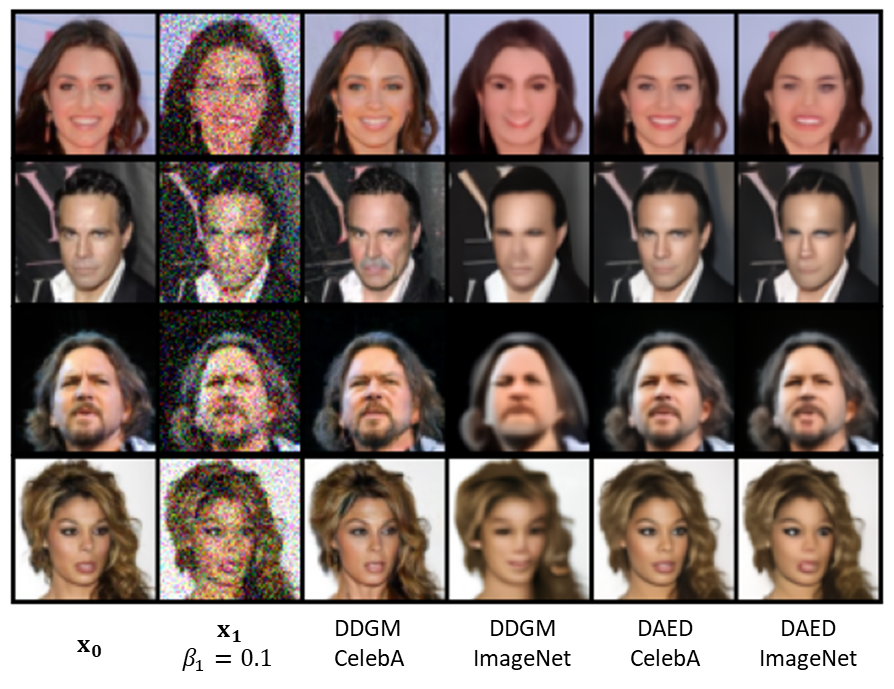
\includegraphics[width=0.56\linewidth, valign=c]{pics/4_daed/experiments/portability.png} & 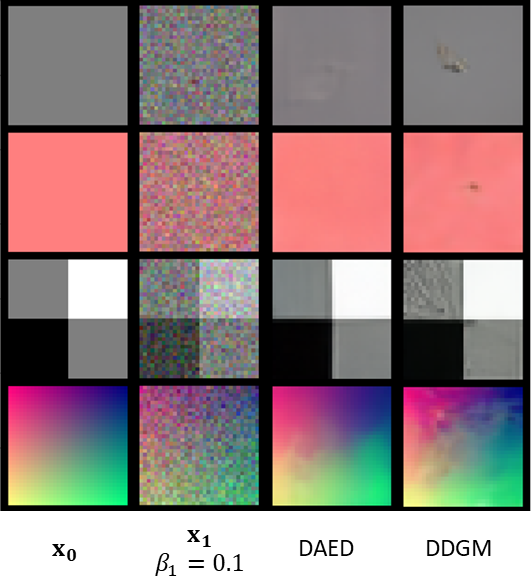
\includegraphics[width=0.38\linewidth, valign=c]{pics/4_daed/experiments/toy_example.png} \\
	    (a) Reconstructions on CelebA & (b) Toy examples
	\end{tabular}
	\caption{(a) Denoising of image with $0.1$ noise using either \ours{} or the corresponding number of the DDGM steps. (b) Four noisy toy examples denoised by \ours{} and the DDGM.}
	\label{fig:transferability}
\end{figure}


% = SECTION =

\section{Conclusion}
In this work, we investigate the generative and denoising capabilities of the Diffusion-based Deep Generative Models. We observe and experimentally validate that it is reasonable to understand DDGMs as a combination of two parts. The first one generates noisy samples from the pure noise by inputting more signal from a learned data distribution, while the second one removes the remaining noise from the signal. Although for standard DDGMs, the exact switching point between those two parts is fluid, we propose a new approach dubbed \ours{} that is explicitly built as a combination of a generative component (a DDGM) and a denoising one (a DAE). 
In the experiments, we observe that \ours{} simplifies training with a standard VLB loss function that leads to improved performance. On the other hand, with increasing noise processed by DAE, \ours{} smoothens the generations resulting in lower performance when training with the simplified objective. 
We further show that DDGMs, and \ours{} especially, generalize well to unseen data, what opens new possibilities for further research in terms of transfer or continual learning of DDGMs.


\part{Properties of Latent Representations}\label{part:2}



% А может, лучшая победа
% Над временем и тяготеньем —
% Пройти, чтоб не оставить следа,
% Пройти, чтоб не оставить тени
    % Марина Ивановна Цветаева

% Женский голос, как ветер, несется,
% Черным кажется, влажным, ночным,
% И чего на лету ни коснется,
% Всё становится сразу иным.
    % Анна Ахматова





\chapter[Alleviating Adversarial Attacks on VAEs with MCMC]{Alleviating Adversarial Attacks\\ on Variational Autoencoders\\ with MCMC}\label{chap:adv_att}
%\begin{verse}
%\textit{
%\hfill This chapter is based on the NeurIPS 2022 paper \citep{kuzina2022alleviating} and ICLR RobustML workshop paper \citep{kuzina2021adv}.
%} 
%\end{verse}
\begin{flushright}
	\small{
		\textit{
			\hfill This chapter is based on the NeurIPS 2022 paper \citep{kuzina2022alleviating} \\
			\hfill 	and ICLR RobustML workshop paper \citep{kuzina2021adv}.
		} 
		
	}
\end{flushright}
\paragraph{Abstract}
Variational autoencoders (VAEs) are latent variable models that can generate complex objects and provide meaningful latent representations. Moreover, they could be further used in downstream tasks such as classification. As previous work has shown, one can easily fool VAEs to produce unexpected latent representations and reconstructions for a visually slightly modified input. Here, we examine several objective functions for adversarial attack construction proposed previously and present a solution to alleviate the effect of these attacks. Our method utilizes the Markov Chain Monte Carlo (MCMC) technique in the inference step that we motivate with a theoretical analysis. Thus, we do not incorporate any extra costs during training, and the performance on non-attacked inputs is not decreased. We validate our approach on a variety of datasets (MNIST, Fashion MNIST, Color MNIST, CelebA) and VAE configurations ($\beta$-VAE, NVAE, $\beta$-TCVAE), and show that our approach consistently improves the model robustness to adversarial attacks.

\newpage
%--------------------------------
% ==== SECTION: Introduction ====
% %--------------------------------
\section{Introduction}\label{sec:intro}

Variational Autoencoders (VAEs) \cite{kingma2014autoencoding, rezende2014stochastic} are latent variable models parameterized by deep neural networks and trained with variational inference. Recently, it has been shown that VAEs with hierarchical structures of latent variables \cite{Ranganath2016-yg}, coupled with skip-connections \cite{Maaloe2019-bp, So_nderby2016-en}, can generate high-quality images \cite{Child2020-ze, Vahdat2020-xe}. An interesting trait of VAEs is that they allow learning meaningful latent space that could be further used in downstream tasks \cite{bengio2013representation, higgins2017darla}. These successes of VAEs motivate us to explore the \textit{robustness} of the resulting latent representations to better understand the capabilities and potential vulnerabilities of VAEs. Here, we focus on \textit{adversarial attacks} on VAEs to verify robustness of latent representations that is especially important in such applications as anomaly detection \cite{an2015variational, Maaloe2019-bp} or data compression \cite{balle2018variational, habibian2019video}. 

The main questions about adversarial attacks for VAEs are mainly focused on how they could be formulated and alleviated. In \cite{Gondim-Ribeiro2018-cu}, it is proposed to minimize the KL-divergence between an adversarial input and a target input to learn an adversarial attack for the vanilla VAE. Further, in \cite{kuzina2021adv}, it is shown that a similar strategy can be used to attack hierarchical VAEs. To counteract the adversarial attacks, the authors of \cite{Willetts2019-mu} suggest using a modified VAE objective, namely, $\beta$-TCVAE, that increases VAE robustness, especially when coupled with a hierarchical structure. It was shown in \cite{camuto2021towards} that $\beta$-VAEs tend to be more robust to adversarial attacks in terms of the $r$-metric proposed therein. The authors of \cite{barrett2021certifiably} presented that the adversarial robustness can be achieved by constraining the Lipschitz constant of the encoder and the decoder. \cite{cemgil2020autoencoding, Cemgil2019-vn} introduced modifications in the VAE framework that allow for better robustness against the adversarial attacks on downstream classification tasks. In our work, we consider $\beta$-VAE, $\beta$-TCVAE and a hierarchical VAE, and outline a defence strategy that improves robustness to attacks on the encoder and the downstream classification task. The proposed method is applied during inference and, therefore, can be combined with other known techniques to get more robust latent representations.


An adversarial attack on a VAE is usually formulated as an additive perturbation $\varepsilon$ of the real data point $\rvx^r$ so that the resulting point is perceived by a model as if it is a totally different image (either during reconstruction or in the downstream classification task) \cite{Gondim-Ribeiro2018-cu}. In Figure \ref{fig:toy_exaple}, we depict an example of an attack on the encoder. The reference point $\rvx^r$ and the adversarial point $\rvx^a$ are almost indistinguishable, but they are encoded into different regions in the latent space. As a result, their reconstructions also differ significantly.

% \begin{wrapfigure}{r}{0.53\textwidth}
\begin{figure}[t]
	% \vskip -100pt
	\begin{center}
		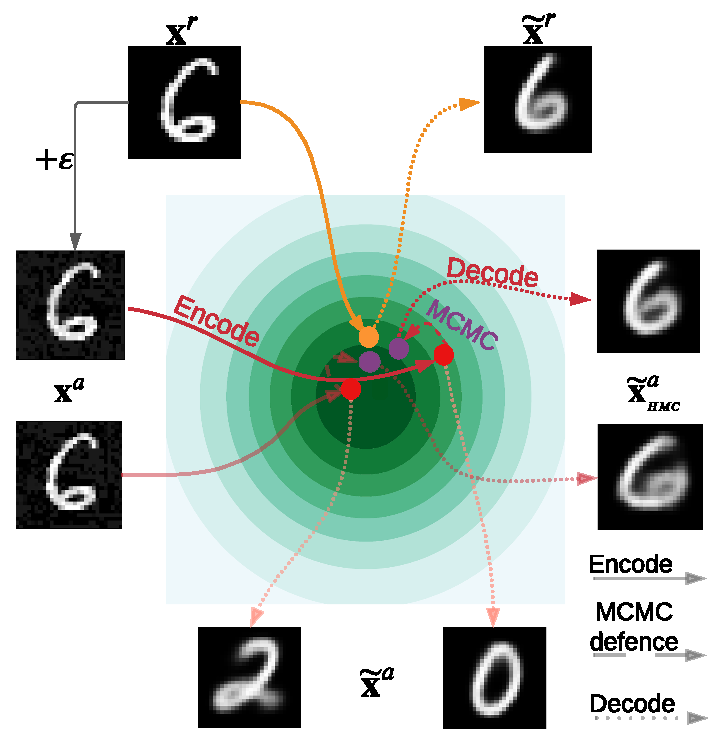
\includegraphics[width=0.6\linewidth]{pics/3_adv_att/Figure_1_upd.pdf}
		\caption{An example of an unsupervised encoder attack on VAE with 2D latent space and the proposed defense. 
			Given a single reference point $\rvx^r$ we learn additive perturbation $\varepsilon$, s.t. perturbed input $\rvx^a$ has the most different latent code and therefore the reconstruction $\widetilde{\rvx}^a$. 
			We observe that a single reference point can be mapped to extremely different regions of the latent space but using MCMC we are able to move them closer to the initial position so that the reconstruction $\widetilde{\rvx}^a_{\text{\tiny{HMC}}}$ is similar to the initial one $\widetilde{\rvx}^r$.}
		\label{fig:toy_exaple}
	\end{center}
\end{figure}
% \end{wrapfigure}

In this paper, we propose the method motivated by the following hypothesis: \textit{An adversarial attack maps the input to a latent region with a lower probability mass assigned by the true posterior (proportional to the conditional likelihood times the marginal over latents) and, eventually, we obtain incorrect reconstructions}. 
Therefore, a potential manner to alleviate the effect of an attack may rely on running a Markov chain to move the latent representation back to a more probable latent region. 
Such a defence is reasonable because we do not modify the training procedure or the model itself, we only insert a correction procedure. As a result, we propose to counteract adversarial attacks by enhancing the variational inference with Markov Chain Monte Carlo (MCMC) sampling. 
The illustrative example depicted in the Figure \ref{fig:toy_exaple} shows that the latent code of the adversarial input (red circle) moves closer to the latent code of the reference point (orange circle) after applying the MCMC (purple circle). 


The contribution of this work is the following:
\begin{itemize}%[leftmargin=*]
    \item We propose to use an MCMC technique during inference to correct adversarial attacks on VAEs.
    \item We show theoretically that the application of an MCMC technique could indeed help to counteract adversarial attacks (Theorem \ref{theorem:main}).
    \item We indicate empirically that the previously proposed strategies to counteract adversarial attacks do not generalize well across various datasets.
    \item We show empirically that the proposed approach (i.e., a VAE with an MCMC during inference) outperforms all baselines by a significant margin.
\end{itemize}

% In Figure \ref{fig:toy_exaple} we show an example of the \textit{supervised} attack on VAE with the 2D latent space. We show that we can add noise $\epsilon$ to a reference image so that the resulting adversarial input (second column) is encoded to a new point in the latent space. This new point is defined by the target image (first column). In \textit{unsupervised} attacks, on the other hand, we assume that the target image is not given. We show that it is still possible to construct an effective attack in this setting. The research goals of this work are the following:
% \begin{itemize}[leftmargin=*]
%     \item Defining robustness measures to understand how VAEs behave for adversarial attacks both in the latent space and the pixel space.
%     \item Assessing robustness of hierarchical and $\beta$-VAEs to adversarial attacks.
%     \item \jt{We need to add a bullet about MCMC to the rescue!}
% \end{itemize}


% %-------------------------------
% % ==== SECTION: Methodology ====
% %-------------------------------


% \section{Methodology}
\section{Background}

% ==== SubSECTION ====
\subsection{Variational Autoencoders}
Let us consider a vector of observable random variables, $\rvx \in \mathcal{X}^{D}$ (e.g., $\mathcal{X} = \mathbb{R}$) sampled from  the empirical distribution $p_{e}(\mathbf{\rvx})$, and vectors of latent variables $\rvz_{k} \in \mathbb{R}^{M_{k}}$, $k=1, 2, \ldots, K$, where $M_k$ is the dimensionality of each latent vector. First, we focus on a model with $K=1$ and the joint distribution $p_{\theta}(\rvx, \rvz) = \Dec{\rvx}{\rvz} p(\rvz)$. The marginal likelihood is then equal to $p_{\theta}(\rvx) = \int p_{\theta}(\rvx, \rvz) \mathrm{d} \rvz$. VAEs exploit variational inference \cite{jordan1999introduction} with a family of variational posteriors $\{\Enc{\rvz}{\rvx}\}$, also referred to as encoders, that results in a tractable objective function, i.e., the Evidence Lower BOund (ELBO): 
%$\mathcal{L}(\phi, \theta)
%    = \E_{p_{e}(\mathbf{\rvx})}\left( \E_{\Enc{\rvz}{\rvx}}\ln \Dec{\rvx}{\rvz} - \KL{\Enc{\rvz}{\rvx}}{p(\rvz)} \right)$. 
 \begin{align}
     \mathcal{L}(\phi, \theta)
     = \E_{p_{e}(\mathbf{\rvx})}\left( \E_{\Enc{\rvz}{\rvx}}\ln \Dec{\rvx}{\rvz} - \KL{\Enc{\rvz}{\rvx}}{p(\rvz)} \right).
 \end{align}

$\beta$-VAE \cite{higgins2016beta} uses a modified objective by weighting the $D_{\text{KL}}$ term by $\beta > 0$.
% \begin{equation}\label{eq:beta_elbo}
%     \mathcal{L}^{\beta}(\phi, \theta)
%     = \E_{p_{e}(\mathbf{\rvx})}\left( \E_{\Enc{\rvz}{\rvx}}\ln \Dec{\rvx}{\rvz} - \beta \KL{\Enc{\rvz}{\rvx}}{p(\rvz)} \right).
% \end{equation}
In the case of $K>1$, we consider a hierarchical latent structure with the generative model of the following form: 
\begin{equation}
    p_{\theta}(\rvx, \rvz_1, \ldots, \rvz_K) = \Dec{\rvx}{\rvz_1, \ldots, \rvz_K} \prod_{k=1}^{K}\Dec{\rvz_{k}}{\rvz_{>k}}.
\end{equation}
There are various possible formulations of the family of variational posteriors. However, here we follow the proposition of \citet{So_nderby2016-en} with the autoregressive inference model, namely, $$\Enc{\rvz_1, \ldots, \rvz_K}{\rvx} = \Enc{\rvz_K}{\rvx}\prod_{k=1}^{K-1}\HEnc{\rvz_k}{\rvz_{>k}, \rvx}.$$
This formulation was used, among others, in NVAE \citep{vahdat2020nvae}. Because of the top-down structure, it allows sharing data-dependent information between the inference model and the generative model.


% ==== SubSECTION ====
\subsection{Adversarial attacks}
\begin{table}[t]
	\caption[][\baselineskip]{Different types of attacks on the VAE. We denote $g_{\theta}(z)$ the deterministic mapping induced by decoder $p_{\theta}(x|z)$ and as $p_{\psi}(y|z)$ classification model in the latent space (downstream task).\\
		\textsuperscript{*} Only used during VAE training}
	\label{tab:attack_variation}
	\begin{center}
		\resizebox{\textwidth}{!}{
			% \begin{small}
			% \begin{sc}
			\begin{tabular}{llcccc}
				\toprule
				& \sc{Reference}  &$f(x)$ & $\Delta\left[A, B\right]$  &  $\|\cdot\|_p$ &  \sc{Type}\\ \midrule
				\multirow{3}{3cm}{Latent Space Attack}
				& \multirow{3}{2cm}{\cite{barrett2021certifiably, Gondim-Ribeiro2018-cu, Willetts2019-mu}}
				& \multirow{3}{*}{$q_{\phi}(\cdot|x)$} &  \multirow{3}{*}{$\KL{A}{B}$}   & \multirow{3}{*}{2} & \multirow{3}{*}{Supervised}\\
				&&&&&\\
				&&&&&\\
				\multirow{3}{3cm}{Unsupervised Encoder Attack}
				& \multirow{3}{2cm}{\cite{kuzina2021adv}}
				& \multirow{3}{*}{$q_{\phi}(\cdot|x)$} 
                    & \multirow{3}{*}{$\mathrm{SKL}\left[A\|B\right]$}   
                    & \multirow{3}{*}{2} 
                    & \multirow{3}{*}{Unsupervised}\\
				&&&&&\\
                    &&&&&\\
				\multirow{3}{3cm}{Targeted Output Attack}
				& \multirow{3}{*}{\cite{Gondim-Ribeiro2018-cu}}
				& \multirow{3}{*}{$g_{\theta}(\tilde{z}), \tilde{z} \sim q_{\phi}(\cdot|x)$}   
                    & \multirow{3}{*}{$\|A - B\|_2^2$}  
                    & \multirow{3}{*}{2} & \multirow{2}{*}{Supervised}\\
				&&&&&\\
                    &&&&&\\
				\multirow{3}{3cm}{Maximum Damage Attack}
				& \multirow{3}{2cm}{\cite{barrett2021certifiably, camuto2021towards}}
				& \multirow{3}{*}{$g_{\theta}(\tilde{z}), \tilde{z} \sim q_{\phi}(\cdot|x)$}   
                    & \multirow{3}{*}{$\|A - B\|_2^2$}  
                    & \multirow{3}{*}{2} 
                    & \multirow{3}{*}{Unsupervised}\\
				&&&&&\\
                    &&&&&\\
				\multirow{4}{3cm}{Projected Gradient Descent Attack\textsuperscript{*}}
				& \multirow{3}{*}{\cite{Cemgil2019-vn}}
				& \multirow{3}{*}{$q_{\phi}(\cdot|x)$} 
                    & \multirow{3}{*}{$\mathcal{WD}\left[A, B\right]$}   
                    & \multirow{3}{*}{$\inf$} 
                    & \multirow{3}{*}{Unsupervised}\\
				&&&&&\\
                    &&&&&\\
				\multirow{2}{3cm}{Adversarial Accuracy}
				& \multirow{2}{*}{\cite{cemgil2020autoencoding, Cemgil2019-vn}}
				& \multirow{2}{*}{$p_{\psi}(y|\tilde{z}), \tilde{z} \sim q_{\phi}(\cdot|x)$}  
                    & \multirow{2}{*}{\sc{Cross Entropy}} 
                    & \multirow{2}{*}{$\inf$} 
                    & \multirow{2}{*}{Unsupervised}\\
				&&&&&\\
				\bottomrule
		\end{tabular}}
		% \end{sc}
		% \end{small}
	\end{center}
	\vskip 15pt
\end{table}


\label{sect:adversarial_attacks}
An \textit{adversarial attack} is a slightly deformed data point that results in an undesired or unpredictable performance of a model \cite{goodfellow2014explaining}. In this work, we focus on the attacks that are constructed as an additive perturbation of the real data point $\rvx^r$ (which we will refer to as \textit{reference}), namely:
\begin{align}
    &\rvx^a = \rvx^r + \varepsilon, \text{where}\\
    &\|\varepsilon\|_{p} \leq \delta ,
\end{align}
where $\delta$ is the radius of the attack. The additive perturbation $\varepsilon$ is chosen in such a way that the attacked point does not differ from the reference point too much in a sense of a given similarity measure. It is a solution to an optimization problem solved by the attacker. The optimization problem could be formulated in various manners by optimizing different objectives and by having specific constraints and/or assumptions.

\paragraph{Attack construction} 
Let $f(x)$ be part of the model available to the attacker. In the case of VAEs, this, for example, may be an encoder network or an encoder with the downstream classifier in the latent space. The attacker uses a similarity measure $\Delta$ to learn an additive perturbation to a reference point. We consider two settings: \textit{unsupervised} and \textit{supervised}. In the former case, the perturbation is supposed to incur the largest possible change in $f$:
\begin{equation}\label{eq:objective_unsup}
    \varepsilon = \arg\max_{\|\varepsilon\|_p \leq \delta }\Delta\left[f(\rvx^r + \varepsilon) , f(\rvx^r) \right].
\end{equation}
The latter setting requires a \textit{target point} $\rvx^t$. The perturbation attempts to match the output for the target and the attacked points, namely:
\begin{equation}\label{eq:objective_sup}
    \varepsilon = \arg\min_{\|\varepsilon\|_p \leq \delta }\Delta\left[ f(\rvx^r + \varepsilon), f(\rvx^t) \right].
\end{equation}
There are different ways to select $f$ and $\Delta$ in the literature. Furthermore, different $L_p$-norms can be used to restrict the radius of the attack. Table \ref{tab:attack_variation} summarizes recent work on the topic. %adversarial attacks on VAE. 

In this work, we focus on attacking the encoder and the downstream classification task using unsupervised adversarial attacks. 
%\mw{I am slightly confused how the description below relates to the text above?}This work focuses on two types of unsupervised attacks\mw{isn't the second one a supervised attack?}: attack on the encoder and the downstream classification task. 
In the former, we maximize the symmetric KL-divergence to get the point with the most unexpected latent code and, therefore, the reconstruction. In the latter case, the latent code is passed to a classifier. The attack is trained to change the class of the point by maximizing the cross-entropy loss. However, the method we propose in Section \ref{sec:defence} is not limited to these setups since it is agnostic to how the attack was trained. 

%%%%%%%%%%%%%%%%%%%%
%-----SubSECTION-----
%%%%%%%%%%%%%%%%%%%%
\paragraph{Robustness measures} 
To measure the robustness of the VAE as well as the success of the proposed defence strategy, we focus on two metrics: $\mathrm{MSSSIM}$ and Adversarial accuracy.
For latent space attacks, we follow \citet{kuzina2021adv} in using Multi-Scale Structural Similarity Index Measure ($\mathrm{MSSSIM}$) \citep{wang2003multiscale}. We calculate $\mathrm{MSSSIM}[\widetilde{\rvx}^{r}, \widetilde{\rvx}^{a}]$, that is, the similarity between the reconstructions of $\rvx^{r}$ and the corresponding $\rvx^{a}$. We do not report the similarity between a reference and the corresponding adversarial input, since this value is the same for all the considered models (for a given attack radius). A successful adversarial attack would have a small value of  $\mathrm{MSSSIM}[\widetilde{\rvx}^{r}, \widetilde{\rvx}^{a}]$. 

For the attacks on the downstream classifier, we follow \citet{cemgil2020autoencoding, Cemgil2019-vn} and calculate the adversarial accuracy. For a given trained VAE model, we first train a linear classifier using latent codes as features. Afterwards, the attack is trained to fool the classifier. Adversarial accuracy is the proportion of points for which the attack was unsuccessful. Namely, when the predicted class of the reference and corresponding adversarial point are the same.  

%%%%%%%%%%%%%%%%%%%%
%-----SubSECTION-----
%%%%%%%%%%%%%%%%%%%%
\section{Preventing adversarial attacks with MCMC} \label{sec:defence}
% \subsection{Preventing adversarial attacks with MCMC}

\paragraph{Assumptions and the hypothesis}

We consider a scenario in which an attacker has access to the VAE encoder and, where relevant, to the downstream classification model. Above, we presented in detail how an attack could be performed. We assume that the defender cannot modify these components, but it is possible to add elements that the attacker has no access to. 

We hypothesize that \textit{the adversarial attacks result in incorrect reconstructions because the latent representation of the adversarial input lands in a region with a lower probability mass assigned by the true posterior. %being proportional to the conditional likelihood and the prior
}
This motivates us to use a method which brings the latents "back" to a highly probable region as a potential defence strategy. 
Since the adversarial attack destroys the input irreversibly, at the first sight it seems impossible to reconstruct the latent representation of the reference point. 
We aim at showing that this is possible to some degree theoretically and empirically (Appendix \ref{appendix:posterior_ratio}). 

\paragraph{The proposed solution } In order to steer the latents towards high probability regions, we propose to utilize an MCMC method during inference time. 
Since we are not allowed to modify the VAE or its learning procedure, this is a reasonable procedure from the defender's perspective. 
Another positive outcome of such an approach is that in a case of no attack, the latents given by the MCMC sampling will be closer to the mean of the posterior, thus, the reconstruction should be sharper or, at least, not worse. 
Note that the variational posterior approximates the true posterior from which the MCMC procedure samples. 
We propose to sample from $q^{(t)}(\rvz|\rvx) = \int Q^{(t)}(\rvz|\rvz_0) q_{\phi}(\rvz_0|\rvx) d\rvz_0$, where $Q^{(t)}(\rvz|\rvz_0)$ is a transition kernel of MCMC with $t$ steps and the target distribution $\pi(\rvz) = p_{\theta}(\rvz|\rvx) \propto p_{\theta}(\rvx|\rvz)p(\rvz)$. 
Alternatively, we can use optimization to find the mode of the posterior, however, MCMC can add extra benefits such as exploration of the typical set and randomness (see Appendix \ref{appendix:hmc_vs_opt} for details).

% Now, the naturally arising question is whether applying the MCMC could indeed help us in the case of an adversarial attack. 
To further analyze the proposed approach, we start with showing the following lemma:

\begin{lemma}\label{lemma:1}
Consider true posterior distributions of the latent code $\rvz$ for a data point $\rvx$ and its corrupted version $\rvx^a$.  
Assume also that $\ln p_{\theta}(\rvz|\rvx)$ is twice differentiable  over $\rvx$ with continuous derivatives at the neighbourhood around $\rvx=\rvx^r$. 
Then the KL-divergence between these two posteriors could be expressed using the small $o$ notation of the radius of the attack, namely:
% Consider true posterior distributions of the latent code $\rvz$ for a data point $\rvx^r$ and its corrupted version $\rvx^a$. Assume also that $\ln p_{\theta}(\rvz|\rvx)$ is differentiable at the point $\rvx = \rvx^r$. Then the KL-divergence between these two posteriors could be expressed using the small $o$ notation in terms of the radius of the attack, namely:
\begin{equation}
     \KL{ p_{\theta}(\rvz|\rvx^r)}{p_{\theta}(\rvz|\rvx^a)} = o(\|\varepsilon\|).
\end{equation}
\end{lemma}
\textit{Proof} See Appendix \ref{appendix:theory}.

According to Lemma \ref{lemma:1}, the difference (in the sense of the Kullback-Leibler divergence) between the true posteriors for a data point $\rvx$ and its corrupted version $\rvx^{a}$ decreases faster than the norm of the attack radius. However, it is important to note that this result is only valid for asymptotically small attack radius.

Next, the crucial step to show is whether we can quantify somehow the difference between the distribution over latents for $\rvx^a$ after running MCMC with $t$ steps, $q^{(t)}(\rvz|\rvx^a)$, and the variational distribution for $\rvx^r$, $q_{\phi}(\rvz|\rvx^r)$. 
We provide an important upper-bound for the Total Variation distance (TV)\footnote{The Total Variation fulfills the triangle inequality and it is a proper distance measure.} between $q^{(t)}(\rvz|\rvx^a)$ and $q_{\phi}(\rvz|\rvx^r)$ in the following lemma:

\begin{lemma}\label{lemma:2}
The Total Variation distance ($\mathrm{TV}$) between the variational posterior with MCMC for a given corrupted point $\rvx^a$, $q^{(t)}(\rvz|\rvx^a)$, and the variational posterior for a given data point $\rvx^r$, $q_{\phi}(\rvz|\rvx^r)$, can be upper bounded by the sum of the following three components:
\begin{align}
\TV{q^{(t)}(\rvz|\rvx^a)}{q_{\phi}(\rvz|\rvx^r)}
\leq &
    \TV{q^{(t)}(\rvz|\rvx^a)}{p_{\theta}(\rvz|\rvx^a)} \notag\\
    &+ 
    \sqrt{\tfrac12 \KL{ p_{\theta}(\rvz|\rvx^r)}{p_{\theta}(\rvz|\rvx^a)} } \notag\\
    &+
   \sqrt{\tfrac12  \KL{q_{\phi}(\rvz|\rvx^r)}{p_{\theta}(\rvz|\rvx^r)} }.
\end{align}
\end{lemma}
\textit{Proof} See Appendix \ref{appendix:theory}.

The difference expressed by $\TV{q^{(t)}(\rvz|\rvx^a)}{q_{\phi}(\rvz|\rvx^r)}$ is thus upper-bounded by the following three components:
\begin{itemize}
    \item The $\mathrm{TV}$ between  $q^{(t)}(\rvz|\rvx^a)$ and the real posterior for the corrupted image, $p_{\theta}(\rvz|\rvx^a)$. Theoretically, if $t \rightarrow \infty$, $q^{(\infty)}(\rvz|\rvx^a) = p_{\theta}(\rvz|\rvx^a)$ and, hence, $\TV{ q^{(\infty)}(\rvz|\rvx^a)}{p_{\theta}(\rvz|\rvx^a) } = 0$.
    \item The second component is the square root of the KL-divergence between the real posteriors for the image and its corrupted counterpart. Lemma \ref{lemma:1} gives us information about this quantity.
    \item The last element, the square root of $\KL{ q_{\phi}(\rvz|\rvx^r)}{p_{\theta}(\rvz|\rvx^r)}$, quantifies the \textit{approximation gap} \cite{cremer2018inference}, i.e., the difference between the best variational posterior from a chosen family, and the true posterior. This quantity has no direct connection with adversarial attacks. However, as we can see, using a rich family of variational posteriors can help us to obtain a tighter upper-bound. In other words, taking flexible variational posteriors allows to counteract attacks. This finding is in line with the papers that propose to use hierarchical VAEs as the means for preventing adversarial attacks \cite{Willetts2019-mu}.
\end{itemize}

Eventually, by applying Lemma \ref{lemma:1} to Lemma \ref{lemma:2}, we obtain the following result:

\begin{theorem}\label{theorem:main}
The upper bound on the total variation distance between samples from MCMC for a given corrupted point $\rvx^a$, $q^{(t)}(\rvz|\rvx^a)$, and the variational posterior for the given real point $\rvx^r$, $q_{\phi}(\rvz|\rvx^r)$, is the following:
\begin{align} \label{eq:theorem_1_main}
    \TV{ q^{(t)}(\rvz|\rvx^a)}{q_{\phi}(\rvz|\rvx^r) }
\leq 
&  \,\TV{ q^{(t)}(\rvz|\rvx^a)}{p_{\theta}(\rvz|\rvx^a) } \notag \\
    &+ 
   \sqrt{\tfrac12  \KL{ q_{\phi}(\rvz|\rvx^r) }{ p_{\theta}(\rvz|\rvx^r)} } \notag\\
   &+ o(\sqrt{\|\varepsilon\|}).
%   \xrightarrow{t\rightarrow \inf}  
%   \sqrt{\tfrac12  \text{KL}\left[ q_{\phi}(\rvz|\rvx) \| p_{\theta}(\rvz|\rvx)\right]} + o(\|\varepsilon\|)
\end{align}
\end{theorem}
\textit{Proof} See Appendix \ref{appendix:theory}.


As discussed already, the first component gets smaller with more steps of the MCMC. %In other words, we can say that it results in the \mw{not so sure this is only variance, as during burn in we also have bias} \textit{variance} (the more steps of the MCMC we apply, the smaller the difference). 
The second component could be treated as a \textit{bias} of the family of variational posteriors. Finally, there is the last element that corresponds to a constant error that is unavoidable. However, this term decays faster than the square root of the attack radius for the asymptotically small attack radius.

\paragraph{Specific implementation of the proposed approach}
In this paper, we use a specific MCMC method, namely, the Hamiltonian Monte Carlo (HMC) \cite{betancourt2017conceptual, duane1987hybrid}. Once the VAE is trained, the attacker calculates an adversarial point $\rvx^a$ using the encoder of the VAE. After the attack, the latent representation of $\rvx^a$ is calculated, $\rvz^a$, and used as the initialization of the HMC.

In the HMC, the target (unnormalized) distribution is $p(\mathbf{x}^{a}|\mathbf{z}) p(\mathbf{z})$. The Hamiltonian is then the energy of the joint distribution of $\rvz$ and the auxilary variable $\rvp$, that is:
\begin{align}
    H(\rvz, \rvp) &= U(\rvz) + K(\rvp),\\
    U(\rvz) &= - \ln p_{\theta}(\mathbf{x}^{a}|\mathbf{z}) - \ln p(\mathbf{z}),\\
    K(\rvp) &= -\tfrac12 \rvp^T\rvp.
\end{align}
When applying the proposed defence to hierarchical models, we update all the latent variables simultaneously. That is, we have $\rvz = \{ \rvz_1, \dots, \rvz_K\}$ and
% \begin{equation}
$U(\rvz) = -\ln \Dec{\rvx^a}{\rvz} - \sum_{k=1}^K\ln p_{\theta}(\rvz_k|\rvz_{k+1}). $
% \end{equation}


\begin{algorithm}
	\caption{One Step of HMC.}
	\label{alg:hmc_step}
	\begin{algorithmic} %[1]
 \\\hrulefill
	   \State \hskip-3mm \textbf{Input}: $\rvz, \eta, L$
		\State $\rvp \sim \mathcal{N}(0,I)$. \Comment{Sample the auxiliary variable }
		\State $\rvz^{(0)} := \rvz, \rvp^{(0)}:=\rvp$.
		\For{$l = 1 \dots, L$} \Comment{Make $L$ steps of \textit{leapfrog}.}
        \State $ \rvp^{(l)} = \rvp^{(l-1)} - \frac{\eta}{2}\nabla_{\rvz} U(\mathbf{z}^{(l)})$.
		\State $\rvz^{(l)} = \rvz^{(l)} + \eta  \nabla_{\rvp} K(\rvp^{(l)})$.
		\State $\rvp^{(l)} = \rvp^{(l)} - \frac{\eta}{2}\nabla_{\rvz} U(\mathbf{z}^{(l)})$.
		\EndFor
		\State $\alpha = \min\left(1, \exp\left(- H(\rvz^{(L)}, \rvp^{(L)}) + H(\rvz^{(0)}, \rvp^{(0)})\right) \right)$
		\State $\rvz =
\begin{cases}
\rvz^{(L)}\, \text{with probability}\, \alpha ,\\
\rvz^{(0)}\, \text{otherwise}.
\end{cases}$  \Comment{Accept a new point with prob. $\alpha$.}
        \State  \hskip-3mm \textbf{Return}: $\rvz$
	\end{algorithmic}
\end{algorithm}

Eventually, the resulting latents from the HMC are decoded. The steps of the whole process are presented below:
\begin{enumerate}%[wide, labelwidth=0pt, labelindent=0pt]
    \item (\textit{Defender}) Train a VAE: $q_{\phi}(\rvz|\rvx)$, $p(\rvz)$, $p_{\theta}(\rvx|\rvz)$.
    \item (\textit{Attacker}) For given $\rvx^r$, calculate the attack $\rvx^{a}$ using the criterion from Eq.~\ref{eq:objective_unsup} or Eq.~\ref{eq:objective_sup}.
    \item (\textit{Defender}) Initialize the latent code $\rvz := \rvz_0$, where $\rvz_{0} \sim q_{\phi}(\rvz|\rvx^{a})$. Then, run $T$ steps of HMC (Algorithm \ref{alg:hmc_step}) with the step size $\eta$ and $L$ \textit{leapfrog} steps.
\end{enumerate}

The resulting latent code $\rvz$ can be passed to the decoder to get a reconstruction or to the downstream classification task.



% %-------------------------------
% % ==== SECTION: Experiments ====
% %-------------------------------

% \newpage
\section{Experiments} \label{sec:experiments}
\subsection{Posterior ratio}\label{sec:exp_ratio}

%\begin{wrapfigure}{r}{0.55\textwidth}
%    \centering
%        \includegraphics[width=0.45\textwidth]{pics/3_adv_att/mnist_posterior_ratio.pdf}
%    \caption{Histograms of the log posterior ratios \textcolor{blue}{before HMC (blue)} and \textcolor{orange}{after HMC (orange)} evaluated on the MNIST dataset.}
%    \label{fig:mnist_post_ratio_main}
%\end{wrapfigure}
\begin{figure}
	\centering
	\includegraphics[width=0.5\textwidth]{pics/3_adv_att/mnist_posterior_ratio.pdf}
	\caption{Histograms of the log posterior ratios \textcolor{blue}{before HMC (blue)} and \textcolor{orange}{after HMC (orange)} evaluated on the MNIST dataset.}
	\label{fig:mnist_post_ratio_main}
\end{figure}

We motivate our method by the hypothesis that the adversarial attack "shifts" a latent code to the region of a lower posterior density, while our approach moves it back to a high posterior probability region. In Section \ref{sec:defence} we theoretically justify our hypothesis, while here we provide an additional empirical evidence.
% In order to verify our claim that applying an MCMC method allows us to counteract attacks by moving a latent code from a region of a lower posterior probability mass to a region of a higher density, we propose to quantify this effect by measuring the ratio of posteriors for $\rvz_1$ and $\rvz_2$. 
The true posterior $p(\rvz | \rvx^{r})$ is not available due to the cumbersome marginal distribution $p(\rvx^{r})$, however, we can calculate the ratio of posteriors because the marginal will cancel out. In our case, we are interested in calculating the posterior ratio between the reference and adversarial latent codes ($\rvz_1 = \rvz^r$,  $\rvz_2 = \rvz^a$) as the baseline, and the posterior ratio between the reference and adversarial code after applying the HMC ($\rvz_1 = \rvz^r$ , $\rvz_2 = \rvz^a_{\text{HMC}}$). The lower the posterior ratio, the better. For practical reasons, we use the logarithm of the posterior ratio since the logarithm does not change the monotonicity and turns products to sums:
\begin{equation}
    \log \text{PR}(\rvz_1, \rvz_2) = \log p_{\theta}(\rvx^r|\rvz_1) + \log p(\rvz_1) - \log p_{\theta}(\rvx^r| \rvz_2) - \log p(\rvz_2) .
\end{equation}
% , namely:

% \begin{align}
% \text{PR}(\rvz_1, \rvz_2) &= \tfrac{p_{\theta}(\rvz_1|\rvx^r)}{p_{\theta}(\rvz_2|\rvx^r)} \\
% &= \tfrac{p_{\theta}(\rvx^r|\rvz_1)p(\rvz_1)}{p_{\theta}(\rvx^r| \rvz_2)p(\rvz_2)} .
% \end{align}
In Figure \ref{fig:mnist_post_ratio_main} we show a plot with two histograms: one with the posterior ratio between the reference and adversarial latent codes ($\rvz_1 = \rvz^r$,  $\rvz_2 = \rvz^a$) in blue, and the second histogram of the posterior ratio between the reference and adversarial code after applying the HMC ($\rvz_1 = \rvz^r$ , $\rvz_2 = \rvz^a_{\text{HMC}}$) in orange. We observe that the histogram has moved to the left after applying the HMC. This indicates that posterior of the adversarial (in the denominator) is increasing when the HMC is used. This is precisely the effect we hoped for and this result provides an empirical evidence in favor of our hypothesis. For more details see \ref{appendix:posterior_ratio}.


% \mw{Max: corrected until here}
% In this section, we experimentally evaluate performance of the proposed approach 
% % \footnote{Our code is publicly available at \url{hidden-repository-due-to-double-blind-review}.}. 
% We perform experiments on a variety of VAE models ($\beta$-VAE, $\beta$-TCVAE and NVAE) and datasets (MNIST. Fashion MNIST, Color MNIST, CelebA).

% ==== SubSECTION ====
\subsection{VAE, $\beta$-VAE and $\beta$-TCVAE} %\texorpdfstring{
% First, we consider attacks on VAE with a single level of latent variables. 
All implementation details and hyperparameters are included in the Appendix ~\ref{appendix:experimental_details} and code repository~\footnote{\url{github.com/AKuzina/defend_vae_mcmc}}. 
\paragraph{Datasets}
VAEs are trained on the MNIST, Fashion MNIST \cite{xiao2017fashion} and Color MNIST datasets. Following \cite{Cemgil2019-vn}, we construct the Color MNIST dataset from MNIST by artificially coloring each image with seven colors (all corners of RGB cube except for black). 

% \begin{wrapfigure}{r}{0.55\textwidth}
\begin{figure}
%\vskip -5pt
    \centering
    \begin{tabular}{ccccc}
        \includegraphics[width=0.1\linewidth]{pics/3_adv_att/mnist_ref_4.pdf} & \includegraphics[width=0.1\linewidth]{pics/3_adv_att/mnist_ref_rec_4.pdf} &
        \includegraphics[width=0.1\linewidth]{pics/3_adv_att/mnist_adv_4.pdf} & \includegraphics[width=0.1\linewidth]{pics/3_adv_att/mnist_adv_rec_4.pdf} & 
        \includegraphics[width=0.1\linewidth]{pics/3_adv_att/mnist_adv_rec_hmc_4.pdf}\\
        \includegraphics[width=0.1\linewidth]{pics/3_adv_att/fashion_mnist_ref_14.pdf} & \includegraphics[width=0.1\linewidth]{pics/3_adv_att/fashion_mnist_ref_rec_14.pdf} &
        \includegraphics[width=0.1\linewidth]{pics/3_adv_att/fashion_mnist_adv_14.pdf} & \includegraphics[width=0.1\linewidth]{pics/3_adv_att/fashion_mnist_adv_rec_14.pdf} & 
        \includegraphics[width=0.1\linewidth]{pics/3_adv_att/fashion_mnist_adv_rec_hmc_14.pdf}\\
        \includegraphics[width=0.1\linewidth]{pics/3_adv_att/color_mnist_ref_4.pdf} & \includegraphics[width=0.1\linewidth]{pics/3_adv_att/color_mnist_ref_rec_4.pdf} &
        \includegraphics[width=0.1\linewidth]{pics/3_adv_att/color_mnist_adv_4.pdf} & \includegraphics[width=0.1\linewidth]{pics/3_adv_att/color_mnist_adv_rec_4.pdf} & 
        \includegraphics[width=0.1\linewidth]{pics/3_adv_att/color_mnist_adv_rec_hmc_4.pdf}\\
        \includegraphics[width=0.1\linewidth]{pics/3_adv_att/color_mnist_ref_9.pdf} & \includegraphics[width=0.1\linewidth]{pics/3_adv_att/color_mnist_ref_rec_9.pdf} &
        \includegraphics[width=0.1\linewidth]{pics/3_adv_att/color_mnist_adv_9.pdf} & \includegraphics[width=0.1\linewidth]{pics/3_adv_att/color_mnist_adv_rec_9.pdf} & 
        \includegraphics[width=0.1\linewidth]{pics/3_adv_att/color_mnist_adv_rec_hmc_9.pdf}\\
        \includegraphics[width=0.1\linewidth]{pics/3_adv_att/celeba_ref_1.png} & \includegraphics[width=0.1\linewidth]{pics/3_adv_att/celeba_ref_rec_1.png} &
        \includegraphics[width=0.1\linewidth]{pics/3_adv_att/celeba_adv_1.png} & \includegraphics[width=0.1\linewidth]{pics/3_adv_att/celeba_adv_rec_1.png} & 
        \includegraphics[width=0.1\linewidth]{pics/3_adv_att/celeba_adv_rec_hmc_1.png}\\
        \includegraphics[width=0.1\linewidth]{pics/3_adv_att/celeba_ref_2.png} & \includegraphics[width=0.1\linewidth]{pics/3_adv_att/celeba_ref_rec_2.png} &
        \includegraphics[width=0.1\linewidth]{pics/3_adv_att/celeba_adv_2.png} & \includegraphics[width=0.1\linewidth]{pics/3_adv_att/celeba_adv_rec_2.png} & 
        \includegraphics[width=0.1\linewidth]{pics/3_adv_att/celeba_adv_rec_hmc_2.png}\\
        (a) $\rvx^r$ & (b) $\widetilde{\rvx}^r$ & (c) $\rvx^a$ & (d) $\widetilde{\rvx}^a$ & (e) $\widetilde{\rvx}^\text{a}_{\text{HMC}}$ \\
    \end{tabular}
    \caption{Examples of (a) reference points, (b) reconstructions of the reference points, (c) adversarial points, (d) reconstructions of the adversarial points, (e) reconstructions of the adversarial points after the proposed defence (HMC). All the adversarial examples are unsupervised attacks on the encoder. Last two rows contain examples for the NVAE model discussed in Section \protect\ref{sec:nvae}}
    \label{fig:adversarial_examples}
    \vspace*{\baselineskip}
\end{figure}
% \end{wrapfigure}


\paragraph{Models}
We train vanilla fully convolutional VAEs, as well as $\beta$-VAE \cite{higgins2016beta} and $\beta$-TCVAE \cite{chen2018isolating, kim2018disentangling}. Both $\beta$-VAE and $\beta$-TCVAE modify the ELBO objective to encourage disentanglement. $\beta$-VAE weighs the KL-term in the ELBO with $\beta > 0$. It is said that the larger values of $\beta$ encourage disentangling of latent representations \cite{chen2018isolating} and improve the model robustness as observed by \cite{camuto2021towards}. $\beta$-TCVAE puts a higher weight on the total correlation (TC) term of the ELBO. Penalization of the total correlation was shown to increase the robustness of VAE adversarial attacks \cite{Willetts2019-mu}.

In Appendix \ref{appendix:beta_vae_param} we provide details of the architecture, optimization, and results on the test dataset for VAE trained with different values of $\beta$. 
We note that the optimal value in terms of the negative log-likelihood (NLL) is always $\beta=1$. Larger values of $\beta$ are supposed to improve robustness in exchange for the reconstruction quality. When evaluating the robustness of $\beta$-VAE and $\beta$-TCVAE, we train models with $\beta \in \{2, 5, 10\}$. Then, we select the value of $\beta$ that provides the most robust model in terms of the used metric. Next, we apply our defence strategy to this model to observe the potential performance improvement. 


\begin{table}[h]
\caption[][\baselineskip]{Results for unsupervised attack with radius $0.1$ and $0.2$ on MNIST and Fashion MNIST datasets. We attack the encoder (left) and the downstream classification task (right).
% Higher values correspond to more robust models.
\\\textsuperscript{$\dagger$} Our implementation.}
\vskip -0.2cm
\label{tab:mnist_attack_result}
\begin{center}
\begin{small}
\begin{sc}
\resizebox{1.0\textwidth}{!}{
\begin{tabular}{lllcc|ccc|ll}
\toprule
& & & \multicolumn{2}{c|}{$\mathrm{MSSSIM}[\widetilde{\rvx}^{r}, \widetilde{\rvx}^{a}]$ $\uparrow$} & \multicolumn{3}{c|}{Adversarial Accuracy $\uparrow$} & \multirow{2}{*}{MSE $\downarrow$}  \\
\multicolumn{3}{c}{$\|\varepsilon\|$} & 0.1 & 0.2 & 0.0 & 0.1 & 0.2           & &\\ 
\midrule
 & \multirow{3}{*}{\STAB{\rotatebox[origin=c]{90}{\small{MNIST}}}} 
 & VAE & 0.70 \tiny{(0.02)} & 0.36 \tiny{(0.03)} & \textbf{0.90} \tiny{(0.04)} & 0.08 \tiny{(0.04)} & 0.05 \tiny{(0.03)} & 578.7 \\
&& \textbf{VAE + HMC} & \textbf{0.88} \tiny{(0.01)} & \textbf{0.76} \tiny{(0.02)} & 0.76 \tiny{(0.01)} & \textbf{0.25} \tiny{(0.03)} & \textbf{0.19} \tiny{(0.03)} & \textbf{478.1} 
\\
&& $\beta$-VAE & 0.75 \tiny{(0.01)} & 0.50 \tiny{(0.03)} & 0.90 \tiny{(0.05)} & 0.11 \tiny{(0.04)} & 0.01 \tiny{(0.01)} & 824.2 \\
&& $\beta$-TCVAE\textsuperscript{$\dagger$} 
& 0.70 \tiny{(0.02)} & 0.46 \tiny{(0.03)} & 0.86 \tiny{(0.05)} & 0.05 \tiny{(0.03)} & 0.03 \tiny{(0.02)} & 828.4
\\ \midrule 
\multirow{3}{*}{\STAB{\rotatebox[origin=c]{90}{\small{Fashion}}}} &\multirow{3}{*}{\STAB{\rotatebox[origin=c]{90}{\small{MNIST}}}} 
&VAE           & 0.59 \tiny{(0.03)} & 0.47 \tiny{(0.03)} & 0.78 \tiny{(0.06)} & 0.00 \tiny{(0.01)} & 0.01 \tiny{(0.01)} & 814.2  \\
&& \textbf{VAE + HMC}    & \textbf{0.66} \tiny{(0.03)} & \textbf{0.54} \tiny{(0.03)} & 0.56 \tiny{(0.01)} & \textbf{0.14} \tiny{(0.02)} & \textbf{0.13} \tiny{(0.02)} & \textbf{764.2} \\ 
&& $\beta$-VAE & 0.52 \tiny{(0.03)} & 0.41 \tiny{(0.03)} & 0.80 \tiny{(0.05)} & 0.00 \tiny{(0.01)} & 0.00 \tiny{(0.01)} & 
1021.1\\
&& $\beta$-TCVAE\textsuperscript{$\dagger$} & 0.52 \tiny{(0.03)} & 0.42 \tiny{(0.03)} & \textbf{0.84} \tiny{(0.05)} & 0.00 \tiny{(0.01)} & 0.02 \tiny{(0.02)} & 980.4\\ 
\bottomrule
\end{tabular}
}
\end{sc}
\end{small}
\end{center}
\vspace*{\baselineskip}
\end{table}

%%%% MOVED TO APPENDIX
% \begin{figure}[t]
%     \centering
%     \begin{tabular}{ll}
%         \includegraphics[width=0.5\textwidth]{img/msssim_eps_1.pdf} & 
%         \includegraphics[width=0.5\textwidth]{img/msssim_eps_2.pdf} \\
%         \multicolumn{1}{c}{(a) $||\varepsilon ||_{\inf} = 0.1$} &
%         \multicolumn{1}{c}{(b) $||\varepsilon ||_{\inf} = 0.2$} \\
%         % (a) & (b) \\
%         % (c) & (d)
%     \end{tabular}
%     \caption{Improvement of the Reconstruction Similarity after the proposed defence. We fix the attack radius to be equal to (a) 0.1 and (b) 0.2. Higher values correspond to a more robust representations.}
%     \vskip -10pt
%     \label{fig:mnist_rec_similarity}
% \end{figure}


\begin{table}[ht]
\caption[][\baselineskip]{Results for unsupervised attack with radius $0.1$ and $0.2$ on ColorMNIST dataset. We attack the encoder (left) and the downstream classification task (right).
% Higher values correspond to more robust models.
\\ \textsuperscript{$\dagger$} Our implementation. \\
\textsuperscript{*} Values reported in \cite{cemgil2020autoencoding}, VAE implementation and evaluation protocol may differ. }
\vskip -0.2cm
\label{tab:color_mnist_attack_results}
\begin{center}
\begin{small}
\begin{sc}
\resizebox{1.03\textwidth}{!}{
\begin{tabular}{lcc|cccccc|ll}
\toprule
 & \multicolumn{2}{c|}{$\mathrm{MSSSIM}[\widetilde{\rvx}^{r}, \widetilde{\rvx}^{a}]$ $\uparrow$} & \multicolumn{6}{c|}{Adversarial Accuracy $\uparrow$} & \multirow{3}{*}{MSE$\downarrow$} &  \multirow{3}{*}{FID $\downarrow$} \\
 &     &     & \multicolumn{3}{c}{Digit} &  \multicolumn{3}{c|}{Color} & & \\
 $\|\varepsilon\|$& 0.1 & 0.2 & 0.0 & 0.1 & 0.2           & 0.0 & 0.1 & 0.2             & & \\ \midrule
% \multirow{9}{*}{\STAB{\rotatebox[origin=c]{90}{Color MNIST}}} & 
VAE & 0.36 \tiny{(0.03)} & 0.19 \tiny{(0.02)} & \textbf{1.00 \tiny{(0.00)}} & 0.04 \tiny{(0.03)} & 0.02 \tiny{(0.02)} & 1.00 \tiny{(0.00)} & 0.06 \tiny{(0.03)} & 0.06 \tiny{(0.03)} & \textbf{261} & \textbf{2.1}\\
% & 
\textbf{VAE + HMC}
& \textbf{0.96 \tiny{(0.01)}} & \textbf{0.90 \tiny{(0.01)}} & 0.42 \tiny{(0.01)} & 0.16 \tiny{(0.02)} & 0.11 \tiny{(0.02)} & 1.00 \tiny{(0.00)} & 0.68 \tiny{(0.03)} & 0.62 \tiny{(0.03)} & \textbf{206} & \textbf{2.1}\\
\midrule
$\beta$-VAE 
& 
0.75 \tiny{(0.01)} & 0.5 \tiny{(0.03)} & 0.88 \tiny{(0.04)} & 0.08 \tiny{(0.04)} & 0.05 \tiny{(0.03)} & 1.00 \tiny{(0.00)} & 0.21 \tiny{(0.06)} & 0.18 \tiny{(0.05)} & 366 & 2.4\\
$\beta$-TCVAE\textsuperscript{$\dagger$} 
& 
0.35 \tiny{(0.02)} & 0.23 \tiny{(0.02)} & 0.94 \tiny{(0.04)} & 0.08 \tiny{(0.04)} & 0.05 \tiny{(0.03)} & 1.00 \tiny{(0.00)} & 0.06 \tiny{(0.03)} & 0.05 \tiny{(0.02)} & 366 & 3.0\\
% & 
$\text{SE}_{0.1}$\textsuperscript{*}
& N/A                & N/A                & 0.94 \tiny{(N/A)}  & 0.89 \tiny{(N/A)}  & 0.02 \tiny{(N/A)}  & 1.00 \tiny{(N/A)}  & 1.00 \tiny{(N/A)}  & 0.22 \tiny{(N/A)}  & 1372 & 13.0\\
% & 
$\text{SE}_{0.2}$\textsuperscript{*}
& N/A                & N/A                & 0.95 \tiny{(N/A)}  & 0.92 \tiny{(N/A)}  & \textbf{0.87 \tiny{(N/A)}}  & 1.00 \tiny{(N/A)}  & 1.00 \tiny{(N/A)}  & \textbf{1.00 \tiny{(N/A)}}  & 1375 & 11.7 \\
% & 
AVAE\textsuperscript{*} 
& N/A                & N/A                & 0.97 \tiny{(N/A)}  & 0.88 \tiny{(N/A)}  & 0.55 \tiny{(N/A)}  & 1.00 \tiny{(N/A)}  & 1.00 \tiny{(N/A)} & 0.88 \tiny{(N/A)}  & 1372 & 15.5\\
% & 
$\text{SE}_{0.1}$-AVAE\textsuperscript{*}
& N/A                & N/A                & 0.97 \tiny{(N/A)}  & \textbf{0.94 \tiny{(N/A)}}  & 0.25 \tiny{(N/A)}  & 1.00 \tiny{(N/A)}  & 1.00 \tiny{(N/A)}  & 0.60 \tiny{(N/A)}  & 1373 & 13.9\\
% & 
$\text{SE}_{0.2}$-AVAE\textsuperscript{*} 
& N/A                & N/A                & 0.98 \tiny{(N/A)}  & \textbf{0.94 \tiny{(N/A)}}  & 0.80 \tiny{(N/A)}  & 1.00 \tiny{(N/A)}  & 1.00 \tiny{(N/A)}  & 0.83 \tiny{(N/A)}  & 1374 & 13.9\\
% & 
AVAE-SS\textsuperscript{*} 
& N/A                & N/A                & 0.94 \tiny{(N/A)}  & 0.73 \tiny{(N/A)}  & 0.21 \tiny{(N/A)}  & 1.00 \tiny{(N/A)}  & 1.00 \tiny{(N/A)}  & 0.57 \tiny{(N/A)}  & 1379 & 12.4\\
\bottomrule
\end{tabular}}
\end{sc}
\end{small}
\end{center}
\vspace*{\baselineskip}
\end{table}

%%%% MOVED TO APPENDIX
% \begin{figure}[t]
%     \centering
%     \begin{tabular}{ll}
%         \includegraphics[width=0.5\textwidth]{img/adv_acc_eps_1.pdf} &
%         \includegraphics[width=0.5\textwidth]{img/adv_acc_eps_2.pdf} \\
%         \multicolumn{1}{c}{(a) $||\varepsilon ||_{\inf} = 0.1$} &
%         \multicolumn{1}{c}{(b) $||\varepsilon ||_{\inf} = 0.2$} \\
%         % (a) & (b) \\
%         % (c) & (d)
%     \end{tabular}
%     % \vskip -10pt
%     \caption{Improvement of the Adversarial Accuracy after proposed defence. We fix the attack radius to be equal to (a) 0.1 and (b) 0.2.}
%     \vskip -10pt
%     \label{fig:mnist_adv_acc}
% \end{figure}
\paragraph{Attacks on the Encoder} 
In the first setup, we assume that the attacker has access to the encoder of the model $\Enc{z}{x}$ {\cite{barrett2021certifiably, Gondim-Ribeiro2018-cu, Willetts2019-mu}. We use the projected gradient descent (PGD) with 50 steps to maximize the symmetric KL-divergence in the unsupervised setting (\eqref{eq:objective_unsup}). We train 10 adversarial attacks (with different random initialization) for each of 50 reference points. See Appendix \ref{appendix:vae_attack} for the details. We report similarity between the reconstruction of the adversarial and reference point as a measure of the robustness (see Section \ref{sect:adversarial_attacks}). 

\paragraph{Attacks on the downstream task} 
In this setup, we examine how the proposed approach can aleviate the effect of the attack on the downstream tasks in the latent space. For this purpose, we follow the procedure from \cite{cemgil2020autoencoding, Cemgil2019-vn}. Once the VAE is trained, we learn a linear classifier using the mean mappings as features. For the MNIST and Fashion MNIST datasets, we have the 10-class classification problem (digits in the former and pieces of clothing in the latter case). For the ColorMNIST dataset, we consider two classification tasks: the digit classification (10 classes), and the color classification (7 classes). We construct the attack to fool the classifier. See Appendix \ref{appendix:vae_attack} for the details.


\paragraph{Results} 
In Tables \ref{tab:mnist_attack_result} and \ref{tab:color_mnist_attack_results}, we compare our method (VAE + HMC) with the vanilla VAE with other methods in the literature. We report more results and the extended comparison in the Appendix \ref{appendix:beta_vae} where we show that our method combined with $\beta$-VAE and $\beta$-TCVAE leads to the increased robustness. For MNIST and Fashion MNIST (Table \ref{tab:mnist_attack_result}), we observe that the vanilla VAE with the HMC is more robust than $\beta$-VAE and $\beta$-TCVAE. The latter model was shown to be more robust to the latent space attack \cite{Willetts2019-mu}. Still, in our experiments (on different datasets), we could not observe the consistent improvement over the vanilla VAE, when using it with a single level of latent variables. 

In Table \ref{tab:color_mnist_attack_results} we report the result on the ColorMNIST dataset. Here, we additionally compare the adversarial accuracy for our method with the Smooth Encoders (SE) and Autoencoding Variational Autoencoder (AVAE) methods \cite{cemgil2020autoencoding, Cemgil2019-vn}.
% We notice that these methods provide higher adversarial accuracy. However, we have also observed a large discrepancy in terms of the MSE and FID scores of the model itself compared to our experiments, which we suspect might be a result of a mistake in \cite{cemgil2020autoencoding, Cemgil2019-vn}.
% \footnote{We have gotten in touch with the authors, who are kindly working with us to address this issue}

Lastly, we would like to highlight that our defence strategy can be also combined with all the above VAE modifications. One advantage of our approach is that it does not require changing the training procedure of a VAE and, as a result, it does not decrease the quality of the generated images. 
Moreover, we can apply the same procedure to reconstruct the non-corrupted points and it will improve the reconstruction error. 
This result can be seen in the Tables \ref{tab:mnist_attack_result} and \ref{tab:color_mnist_attack_results} and it goes in line with the results of the \cite{salimans2015markov}, where MCMC was used to improve the VAE performance. 
% SE and AVAE methods without any restrictions.  
% Another advantage of our approach is that it does not require changing the training procedure of a VAE and, as a result, it does not decrease the quality of the generated images. \ak{As we observe from the columns \textbf{MSE} and \textbf{FID}, the quality of the vanilla VAE is always better compared to the models with modified training objectives. MODIFY: Mention bridging the gap paper.} We depict several examples of the reconstructions of the attacked point in Figure \ref{fig:adversarial_examples}.


% In Figure \ref{fig:mnist_rec_similarity}, we show how similarity between the reconstructions of the reference and adversarial points increases after the proposed defence is applied. This metric consistently improves for all the datasets, radii and models considered. In Figure \ref{fig:adversarial_examples}, we plot examples for each of the datasets considered (see subsection \ref{sec:nvae} for more details on CelebA experiments). The first two columns contain reference points and their reconstructions (columns a \& b). Then we plot the adversarial input (column c) and its reconstruction without the defence (column d). Finally, we provide the reconstruction with the defence applied (column e) that is much closer to the reconstruction of the reference point.
 


% ==== SubSECTION ====
\begin{figure}[t]
    % \centering
    \begin{adjustbox}{center}
    \begin{tabular}{llll}
        \includegraphics[width=0.4\textwidth]{pics/3_adv_att/nvae_mnist_eps_1.pdf} & 
        \includegraphics[width=0.4\textwidth]{pics/3_adv_att/nvae_mnist_eps_2.pdf} \\
        \multicolumn{2}{c}{\small (a) The reconstruction similarity for MNIST} \\ \\
        \includegraphics[width=0.4\textwidth]{pics/3_adv_att/nvae_celeba_eps_1.pdf} & 
        \includegraphics[width=0.4\textwidth]{pics/3_adv_att/nvae_celeba_eps_2.pdf}\\
         \multicolumn{2}{c}{\small (b) The reconstruction similarity for CelebA}\\
    \end{tabular}
    \end{adjustbox}
    \caption[][\baselineskip]{The robustness improvement for the hierarchical model (NVAE) on (a) MNIST and (b) CelebA for two different attack radii. Higher values correspond to more robust representations.}
    \label{fig:nvae_res}
\end{figure}

\subsection{Hierarchical VAE: NVAE}\label{sec:nvae}

\paragraph{Model and datasets} In this section, we explore the robustness of the deep hierarchical VAE (NVAE) \cite{Vahdat2020-xe}, a specific implementation of a hierarchical VAE that works well for high-dimensional data. We attack models trained on MNIST and CelebA \cite{liu2015faceattributes} datasets. We use the weights of the pre-trained model provided in the official NVAE implementation\footnote{The code and model weights were taken from \url{github.com/NVlabs/NVAE}}. 

\paragraph{Attacks construction}
Following \cite{kuzina2021adv} we construct adversarial attacks on the hierarchical VAE by considering higher-level latent variables. That being said, we use latent variables $\{\rvz_{L-k_A}, \rvz_{L-k_A+1}, \dots, \rvz_L\}$ when constructing an attack (\eqref{eq:objective_unsup}). Otherwise, we follow the same procedure we used for VAEs with a single level of latent variables. We assume that the attacker has access to the model's encoder and uses the symmetric KL-divergence as the objective. The radius of an attack is measured with the $L_{\inf}$ norm. For optimization, we use the projected gradient descent with the number of iterations limited to 50 per point. Further details are reported in the Appendix \ref{appendix:vae_attack}.


\paragraph{Results}
In Figure \ref{fig:nvae_res}, we present reconstruction similarity of the reference and adversarial points for both datasets. We observe that the proposed method consistently improves the robustness of the model to the adversarial attack. This result is in line with our theoretical considerations where a flexible class of variational posteriors could help to counteract adversarial attacks and, eventually, deacrease the bias of the class of models measured in terms of the KL-divergence. Additionally, applying the MCMC can further help us to counteract the attack. In Figure \ref{fig:adversarial_examples} (the two bottom rows), we show how an adversarial point (c) is reconstructed without any defence (d) and with the proposed defence (e). In the depicted samples, we have used the top 10 latent variables ($k_A = 10$) to construct the attack with a radius of 0.05. 



% \begin{wrapfigure}{r}{0.62\textwidth}
\begin{figure}[t]
    \centering
    \begin{tabular}{cc}
     \includegraphics[width=0.4\linewidth]{pics/3_adv_att/attack_mcmc_0_100.pdf} &
     \includegraphics[width=0.4\linewidth]{pics/3_adv_att/attack_mcmc_1_100.pdf} \\
     \multirow{2}{0.45\linewidth}{\centering \small (a) An attacker does not know the defence strategy}&
     \multirow{2}{0.45\linewidth}{\centering \small (b) An attacker knows the defence strategy }\\
     \\
    \end{tabular}
    \caption{Robustness to adversarial attack (with HMC defence). We report similarity of the reference and adversarial point (blue) and their reconstructions (orange).}
    \label{fig:attack_mcmc}
	\vspace*{\baselineskip}
\end{figure}

% \end{wrapfigure}


\subsection{Ablation Study: What if the attacker knows the defence strategy?} \label{sec:ablation}
In our experiments, we rely on the assumption that the attacker does not take into account the defence strategy that we use. We believe that it is reasonable, since the defence requires access to the decoder part of the model, $p_{\theta}(x|z)$, which is not necessarily available to the attacker. 

In this ablation study we verify how the robustness results change if we construct the attack with the access to the defence strategy. We train an adversarial attack with the modified objective \ref{eq:objective_unsup}, which takes into account the HMC step. See Appendix \ref{appendix:attack_mcmc} for more details on the experimental setup. 

In Figure \ref{fig:attack_mcmc} we show the experiment results for various attack radii between 0 and 1. We observe that constructing an attack with such an objective is much harder (Figure \ref{fig:attack_mcmc} (b)).  

% In both cases the reconstructions are almost as close as the initial points, which proves the defence strategy to be successful for this experiment.

% Here we consider the most straightforward approach to construct an attack, which is aligned with the previous works on attacking VAEs. 

% It is, however, possible to use more sophisticated adaptive methods \cite{tramer2020adaptive, athalye2018obfuscated}. We are not aware of the works where such attacks were applied to VAEs and believe that it is an interesting direction for the future work on the topic. 


% \ak{add reference to papers with MCMC defence and attacks, explain that it is out of scope of this paper.}
% In Appendix \ref{appendix:attack_mcmc} we report results of the ablation study, where attacks on the encoder are constructed assuming that the attacker knows the defence strategy and attempts to use it during the attack construction. We observe that using MCMC during the attack construction does not help the attacker. On the contrary, it becomes harder to find a reasonable additive perturbation of the input.





\section{Discussion}
Following the previous works on attacking VAEs \cite{barrett2021certifiably, camuto2021towards, cemgil2020autoencoding, Cemgil2019-vn, Gondim-Ribeiro2018-cu, Willetts2019-mu}, we only consider the projected gradient descent as a way to construct the attack. However, more sophisticated adaptive methods \cite{ athalye2018obfuscated, tramer2020adaptive} were proposed to attack discriminative model and can be potentially applied to VAEs as well.
% We are not aware of the works where such attacks were applied to VAEs and 
We believe that it is an interesting direction for the future work. 

\paragraph{Objective Function}
For the unsupervised attack on the encoder, we use the symmetric KL-divergence to measure the dissimilarity. However, other options are possible, e.g., the forward or reverse KL-divergence or even $L_2$ distance between the means (see Table \ref{tab:attack_variation}). In our comparative experiments (see Appendix \ref{appendix:objectives}), we observe that no single objective consistently performs better than others.

% \paragraph{What if attacker knows the defence strategy?}
% In Appendix \ref{appendix:attack_mcmc} we report results of the ablation study, where attacks on the encoder are constructed assuming that the attacker knows the defence strategy and attempts to use it during the attack construction. We observe that using MCMC during the attack construction does not help the attacker. On the contrary, it becomes harder to find a reasonable additive perturbation of the input.

\paragraph{Attack radius}
During the attack construction we seek to obtain a point that will have the most different latent representation or a different predicted class. However, it is also important that the point itself is as similar to the initial reference point as possible. In Appendix \ref{appendix:attack_radius}, we visualize how the attacks of different radii influence the similarity between the adversarial and reference points. Based on these results, we have chosen the radii which do not allow adversarial points to deviate a lot from the reference (as measured by \textsc{MSSSIM}): $\|\varepsilon\|_{\inf} \leq 0.2$ for the MNIST dataset (which goes in line with the previous works \cite{cemgil2020autoencoding, Cemgil2019-vn}) and $\|\varepsilon\|_{\inf} \leq 0.1$ for the CelebA dataset. 


%\begin{wrapfigure}{r}{0.54\textwidth}
%\vskip -10pt
%    % \centering
%    \begin{tabular}{c}
%        \includegraphics[width=0.8\linewidth]{pics/3_adv_att/hmc_steps_time_ref_rec_sim.pdf} \\
%        % \includegraphics[width=\linewidth]{img/hmc_steps_time_adv_acc.pdf} \\ 
%    \end{tabular}
%    \vskip -5pt
%    \caption{Trade-off between robustness and inference time.}
%    \label{fig:time_vs_performance}
%\end{wrapfigure}


\paragraph{Number of MCMC steps and Inference Time}
In our approach, we have to select the number of MCMC steps that the defender performs. This parameter potentially can be critical as it influences both the inference time (see Appendix \ref{appendix:inference_time}) and the performance (see Appendix \ref{appendix:hmc_steps}). 
In Figure \ref{fig:time_vs_performance} we show the trade-off between the reconstruction similarity and the inference time. The increase in the inference time is cause by a larger number of HMC steps used (we consider 0, 100, 500 and 1000 steps for this experiment).
\begin{marginfigure}
	\vspace*{-8\baselineskip}
	\includegraphics[width=\linewidth]{pics/3_adv_att/hmc_steps_time_ref_rec_sim.pdf} 
	\caption{Trade-off between robustness and inference time.}
	\label{fig:time_vs_performance}
\end{marginfigure}

% In our approach, we have to select the number of MCMC steps that the defender performs. This parameter potentially can be critical \upd{as it influences the inference time (see Appendix \ref{appendix:inference_time}}. Following the theoretical analysis, the more steps in the MCMC procedure is taken, the tighter the bound (\ref{eq:theorem_1_main}) is. On the other hand, typically we have time and computational constraints to take into account. In Appendix \ref{appendix:hmc_steps}, we show the method's performance for the number of HMC steps ranging between 0 and 2000. There is a considerable jump in robustness between 0 and 100 steps. At the same time, we do not observe much improvement as we continue to increase the number of steps. 

\section{Conclusion}
In this work, we explore the robustness of VAEs to adversarial attacks.  We propose a theoretically justified method that allows alleviating the effect of attacks on the latent representations by improving the reconstructions of the adversarial inputs and the downstream tasks accuracy. We experimentally validate our approach on a variety of datasets: both grey-scale (MNIST, Fashion MNIST) and colored (ColorMNIST, CelebA) data. We show that the proposed method improves the robustness of the vanilla VAE models and its various modifications, i.e., $\beta$-VAE, $\beta$-TCVAE and NVAE.




% Видишь, августовские любовники пробегают внизу с цветами,
% голубые струи реклам бесконечно стекают с крыш,
% вот ты смотришь вниз, никогда не меняйся местами,
% никогда ни с кем, это ты себе говоришь.
    % Иосиф Бродский
%%%%%%%% ICML 2021 EXAMPLE LATEX SUBMISSION FILE %%%%%%%%%%%%%%%%%

% \documentclass{article}

% % Recommended, but optional, packages for figures and better typesetting:
% \usepackage{microtype}
% \usepackage{graphicx}
% \usepackage{subfigure}
% \usepackage{booktabs} % for professional tables
% \usepackage{tabularx}

% % hyperref makes hyperlinks in the resulting PDF.
% % If your build breaks (sometimes temporarily if a hyperlink spans a page)
% % please comment out the following usepackage line and replace
% % \usepackage{icml2021} with \usepackage[nohyperref]{icml2021} above.
% \usepackage{hyperref}

% \newcolumntype{Y}{>{\centering\arraybackslash}X}

% % Attempt to make hyperref and algorithmic work together better:
% \newcommand{\theHalgorithm}{\arabic{algorithm}}
% \usepackage{algpseudocode}
% % Use the following line for the initial blind version submitted for review:
% % \usepackage{icml2021}
% % If accepted, instead use the following line for the camera-ready submission:
% \usepackage[accepted]{icml2022}

% % ------------------------------------------------------
% %%%%% NEW MATH DEFINITIONS %%%%%

\usepackage{amsmath,amsfonts,bm}

% Mark sections of captions for referring to divisions of figures
\newcommand{\figleft}{{\em (Left)}}
\newcommand{\figcenter}{{\em (Center)}}
\newcommand{\figright}{{\em (Right)}}
\newcommand{\figtop}{{\em (Top)}}
\newcommand{\figbottom}{{\em (Bottom)}}
\newcommand{\captiona}{{\em (a)}}
\newcommand{\captionb}{{\em (b)}}
\newcommand{\captionc}{{\em (c)}}
\newcommand{\captiond}{{\em (d)}}

% Highlight a newly defined term
\newcommand{\newterm}[1]{{\bf #1}}


% Figure reference, lower-case.
\def\figref#1{figure~\ref{#1}}
% Figure reference, capital. For start of sentence
\def\Figref#1{Figure~\ref{#1}}
\def\twofigref#1#2{figures \ref{#1} and \ref{#2}}
\def\quadfigref#1#2#3#4{figures \ref{#1}, \ref{#2}, \ref{#3} and \ref{#4}}
% Section reference, lower-case.
\def\secref#1{section~\ref{#1}}
% Section reference, capital.
\def\Secref#1{Section~\ref{#1}}
% Reference to two sections.
\def\twosecrefs#1#2{sections \ref{#1} and \ref{#2}}
% Reference to three sections.
\def\secrefs#1#2#3{sections \ref{#1}, \ref{#2} and \ref{#3}}
% Reference to an equation, lower-case.
\def\eqref#1{equation~\ref{#1}}
% Reference to an equation, upper case
\def\Eqref#1{Equation~\ref{#1}}
% A raw reference to an equation---avoid using if possible
\def\plaineqref#1{\ref{#1}}
% Reference to a chapter, lower-case.
\def\chapref#1{chapter~\ref{#1}}
% Reference to an equation, upper case.
\def\Chapref#1{Chapter~\ref{#1}}
% Reference to a range of chapters
\def\rangechapref#1#2{chapters\ref{#1}--\ref{#2}}
% Reference to an algorithm, lower-case.
\def\algref#1{algorithm~\ref{#1}}
% Reference to an algorithm, upper case.
\def\Algref#1{Algorithm~\ref{#1}}
\def\twoalgref#1#2{algorithms \ref{#1} and \ref{#2}}
\def\Twoalgref#1#2{Algorithms \ref{#1} and \ref{#2}}
% Reference to a part, lower case
\def\partref#1{part~\ref{#1}}
% Reference to a part, upper case
\def\Partref#1{Part~\ref{#1}}
\def\twopartref#1#2{parts \ref{#1} and \ref{#2}}

\def\ceil#1{\lceil #1 \rceil}
\def\floor#1{\lfloor #1 \rfloor}
\def\1{\bm{1}}
\newcommand{\train}{\mathcal{D}}
\newcommand{\valid}{\mathcal{D_{\mathrm{valid}}}}
\newcommand{\test}{\mathcal{D_{\mathrm{test}}}}

\def\eps{{\epsilon}}


% Random variables
\def\reta{{\textnormal{$\eta$}}}
\def\ra{{\textnormal{a}}}
\def\rb{{\textnormal{b}}}
\def\rc{{\textnormal{c}}}
\def\rd{{\textnormal{d}}}
\def\re{{\textnormal{e}}}
\def\rf{{\textnormal{f}}}
\def\rg{{\textnormal{g}}}
\def\rh{{\textnormal{h}}}
\def\ri{{\textnormal{i}}}
\def\rj{{\textnormal{j}}}
\def\rk{{\textnormal{k}}}
\def\rl{{\textnormal{l}}}
% rm is already a command, just don't name any random variables m
\def\rn{{\textnormal{n}}}
\def\ro{{\textnormal{o}}}
\def\rp{{\textnormal{p}}}
\def\rq{{\textnormal{q}}}
\def\rr{{\textnormal{r}}}
\def\rs{{\textnormal{s}}}
\def\rt{{\textnormal{t}}}
\def\ru{{\textnormal{u}}}
\def\rv{{\textnormal{v}}}
\def\rw{{\textnormal{w}}}
\def\rx{{\textnormal{x}}}
\def\ry{{\textnormal{y}}}
\def\rz{{\textnormal{z}}}

% Random vectors
\def\rvepsilon{{\mathbf{\epsilon}}}
\def\rvtheta{{\mathbf{\theta}}}
\def\rva{{\mathbf{a}}}
\def\rvb{{\mathbf{b}}}
\def\rvc{{\mathbf{c}}}
\def\rvd{{\mathbf{d}}}
\def\rve{{\mathbf{e}}}
\def\rvf{{\mathbf{f}}}
\def\rvg{{\mathbf{g}}}
\def\rvh{{\mathbf{h}}}
\def\rvu{{\mathbf{i}}}
\def\rvj{{\mathbf{j}}}
\def\rvk{{\mathbf{k}}}
\def\rvl{{\mathbf{l}}}
\def\rvm{{\mathbf{m}}}
\def\rvn{{\mathbf{n}}}
\def\rvo{{\mathbf{o}}}
\def\rvp{{\mathbf{p}}}
\def\rvq{{\mathbf{q}}}
\def\rvr{{\mathbf{r}}}
\def\rvs{{\mathbf{s}}}
\def\rvt{{\mathbf{t}}}
\def\rvu{{\mathbf{u}}}
\def\rvv{{\mathbf{v}}}
\def\rvw{{\mathbf{w}}}
\def\rvx{{\mathbf{x}}}
\def\rvy{{\mathbf{y}}}
\def\rvz{{\mathbf{z}}}

% Elements of random vectors
\def\erva{{\textnormal{a}}}
\def\ervb{{\textnormal{b}}}
\def\ervc{{\textnormal{c}}}
\def\ervd{{\textnormal{d}}}
\def\erve{{\textnormal{e}}}
\def\ervf{{\textnormal{f}}}
\def\ervg{{\textnormal{g}}}
\def\ervh{{\textnormal{h}}}
\def\ervi{{\textnormal{i}}}
\def\ervj{{\textnormal{j}}}
\def\ervk{{\textnormal{k}}}
\def\ervl{{\textnormal{l}}}
\def\ervm{{\textnormal{m}}}
\def\ervn{{\textnormal{n}}}
\def\ervo{{\textnormal{o}}}
\def\ervp{{\textnormal{p}}}
\def\ervq{{\textnormal{q}}}
\def\ervr{{\textnormal{r}}}
\def\ervs{{\textnormal{s}}}
\def\ervt{{\textnormal{t}}}
\def\ervu{{\textnormal{u}}}
\def\ervv{{\textnormal{v}}}
\def\ervw{{\textnormal{w}}}
\def\ervx{{\textnormal{x}}}
\def\ervy{{\textnormal{y}}}
\def\ervz{{\textnormal{z}}}

% Random matrices
\def\rmA{{\mathbf{A}}}
\def\rmB{{\mathbf{B}}}
\def\rmC{{\mathbf{C}}}
\def\rmD{{\mathbf{D}}}
\def\rmE{{\mathbf{E}}}
\def\rmF{{\mathbf{F}}}
\def\rmG{{\mathbf{G}}}
\def\rmH{{\mathbf{H}}}
\def\rmI{{\mathbf{I}}}
\def\rmJ{{\mathbf{J}}}
\def\rmK{{\mathbf{K}}}
\def\rmL{{\mathbf{L}}}
\def\rmM{{\mathbf{M}}}
\def\rmN{{\mathbf{N}}}
\def\rmO{{\mathbf{O}}}
\def\rmP{{\mathbf{P}}}
\def\rmQ{{\mathbf{Q}}}
\def\rmR{{\mathbf{R}}}
\def\rmS{{\mathbf{S}}}
\def\rmT{{\mathbf{T}}}
\def\rmU{{\mathbf{U}}}
\def\rmV{{\mathbf{V}}}
\def\rmW{{\mathbf{W}}}
\def\rmX{{\mathbf{X}}}
\def\rmY{{\mathbf{Y}}}
\def\rmZ{{\mathbf{Z}}}

% Elements of random matrices
\def\ermA{{\textnormal{A}}}
\def\ermB{{\textnormal{B}}}
\def\ermC{{\textnormal{C}}}
\def\ermD{{\textnormal{D}}}
\def\ermE{{\textnormal{E}}}
\def\ermF{{\textnormal{F}}}
\def\ermG{{\textnormal{G}}}
\def\ermH{{\textnormal{H}}}
\def\ermI{{\textnormal{I}}}
\def\ermJ{{\textnormal{J}}}
\def\ermK{{\textnormal{K}}}
\def\ermL{{\textnormal{L}}}
\def\ermM{{\textnormal{M}}}
\def\ermN{{\textnormal{N}}}
\def\ermO{{\textnormal{O}}}
\def\ermP{{\textnormal{P}}}
\def\ermQ{{\textnormal{Q}}}
\def\ermR{{\textnormal{R}}}
\def\ermS{{\textnormal{S}}}
\def\ermT{{\textnormal{T}}}
\def\ermU{{\textnormal{U}}}
\def\ermV{{\textnormal{V}}}
\def\ermW{{\textnormal{W}}}
\def\ermX{{\textnormal{X}}}
\def\ermY{{\textnormal{Y}}}
\def\ermZ{{\textnormal{Z}}}

% Vectors
\def\vzero{{\bm{0}}}
\def\vone{{\bm{1}}}
\def\vmu{{\bm{\mu}}}
\def\vtheta{{\bm{\theta}}}
\def\vepsilon{{\bm{\varepsilon}}}
\def\vzero{{\bm{0}}}
\def\vone{{\bm{1}}}
\def\vmu{{\bm{\mu}}}
\def\vtheta{{\bm{\theta}}}
\def\va{{\bm{a}}}
\def\vb{{\bm{b}}}
\def\vc{{\bm{c}}}
\def\vd{{\bm{d}}}
\def\ve{{\bm{e}}}
\def\vf{{\bm{f}}}
\def\vg{{\bm{g}}}
\def\vh{{\bm{h}}}
\def\vi{{\bm{i}}}
\def\vj{{\bm{j}}}
\def\vk{{\bm{k}}}
\def\vl{{\bm{l}}}
\def\vm{{\bm{m}}}
\def\vn{{\bm{n}}}
\def\vo{{\bm{o}}}
\def\vp{{\bm{p}}}
\def\vq{{\bm{q}}}
\def\vr{{\bm{r}}}
\def\vs{{\bm{s}}}
\def\vt{{\bm{t}}}
\def\vu{{\bm{u}}}
\def\vv{{\bm{v}}}
\def\vw{{\bm{w}}}
\def\vx{{\bm{x}}}
\def\vy{{\bm{y}}}
\def\vz{{\bm{z}}}

% Elements of vectors
\def\evalpha{{\alpha}}
\def\evbeta{{\beta}}
\def\evepsilon{{\epsilon}}
\def\evlambda{{\lambda}}
\def\evomega{{\omega}}
\def\evmu{{\mu}}
\def\evpsi{{\psi}}
\def\evsigma{{\sigma}}
\def\evtheta{{\theta}}
\def\eva{{a}}
\def\evb{{b}}
\def\evc{{c}}
\def\evd{{d}}
\def\eve{{e}}
\def\evf{{f}}
\def\evg{{g}}
\def\evh{{h}}
\def\evi{{i}}
\def\evj{{j}}
\def\evk{{k}}
\def\evl{{l}}
\def\evm{{m}}
\def\evn{{n}}
\def\evo{{o}}
\def\evp{{p}}
\def\evq{{q}}
\def\evr{{r}}
\def\evs{{s}}
\def\evt{{t}}
\def\evu{{u}}
\def\evv{{v}}
\def\evw{{w}}
\def\evx{{x}}
\def\evy{{y}}
\def\evz{{z}}

% Matrix
\def\mA{{\bm{A}}}
\def\mB{{\bm{B}}}
\def\mC{{\bm{C}}}
\def\mD{{\bm{D}}}
\def\mE{{\bm{E}}}
\def\mF{{\bm{F}}}
\def\mG{{\bm{G}}}
\def\mH{{\bm{H}}}
\def\mI{{\bm{I}}}
\def\mJ{{\bm{J}}}
\def\mK{{\bm{K}}}
\def\mL{{\bm{L}}}
\def\mM{{\bm{M}}}
\def\mN{{\bm{N}}}
\def\mO{{\bm{O}}}
\def\mP{{\bm{P}}}
\def\mQ{{\bm{Q}}}
\def\mR{{\bm{R}}}
\def\mS{{\bm{S}}}
\def\mT{{\bm{T}}}
\def\mU{{\bm{U}}}
\def\mV{{\bm{V}}}
\def\mW{{\bm{W}}}
\def\mX{{\bm{X}}}
\def\mY{{\bm{Y}}}
\def\mZ{{\bm{Z}}}
\def\mBeta{{\bm{\beta}}}
\def\mPhi{{\bm{\Phi}}}
\def\mLambda{{\bm{\Lambda}}}
\def\mSigma{{\bm{\Sigma}}}

% Tensor
\DeclareMathAlphabet{\mathsfit}{\encodingdefault}{\sfdefault}{m}{sl}
\SetMathAlphabet{\mathsfit}{bold}{\encodingdefault}{\sfdefault}{bx}{n}
\newcommand{\tens}[1]{\bm{\mathsfit{#1}}}
\def\tA{{\tens{A}}}
\def\tB{{\tens{B}}}
\def\tC{{\tens{C}}}
\def\tD{{\tens{D}}}
\def\tE{{\tens{E}}}
\def\tF{{\tens{F}}}
\def\tG{{\tens{G}}}
\def\tH{{\tens{H}}}
\def\tI{{\tens{I}}}
\def\tJ{{\tens{J}}}
\def\tK{{\tens{K}}}
\def\tL{{\tens{L}}}
\def\tM{{\tens{M}}}
\def\tN{{\tens{N}}}
\def\tO{{\tens{O}}}
\def\tP{{\tens{P}}}
\def\tQ{{\tens{Q}}}
\def\tR{{\tens{R}}}
\def\tS{{\tens{S}}}
\def\tT{{\tens{T}}}
\def\tU{{\tens{U}}}
\def\tV{{\tens{V}}}
\def\tW{{\tens{W}}}
\def\tX{{\tens{X}}}
\def\tY{{\tens{Y}}}
\def\tZ{{\tens{Z}}}


% Graph
\def\gA{{\mathcal{A}}}
\def\gB{{\mathcal{B}}}
\def\gC{{\mathcal{C}}}
\def\gD{{\mathcal{D}}}
\def\gE{{\mathcal{E}}}
\def\gF{{\mathcal{F}}}
\def\gG{{\mathcal{G}}}
\def\gH{{\mathcal{H}}}
\def\gI{{\mathcal{I}}}
\def\gJ{{\mathcal{J}}}
\def\gK{{\mathcal{K}}}
\def\gL{{\mathcal{L}}}
\def\gM{{\mathcal{M}}}
\def\gN{{\mathcal{N}}}
\def\gO{{\mathcal{O}}}
\def\gP{{\mathcal{P}}}
\def\gQ{{\mathcal{Q}}}
\def\gR{{\mathcal{R}}}
\def\gS{{\mathcal{S}}}
\def\gT{{\mathcal{T}}}
\def\gU{{\mathcal{U}}}
\def\gV{{\mathcal{V}}}
\def\gW{{\mathcal{W}}}
\def\gX{{\mathcal{X}}}
\def\gY{{\mathcal{Y}}}
\def\gZ{{\mathcal{Z}}}

% Sets
\def\sA{{\mathbb{A}}}
\def\sB{{\mathbb{B}}}
\def\sC{{\mathbb{C}}}
\def\sD{{\mathbb{D}}}
% Don't use a set called E, because this would be the same as our symbol
% for expectation.
\def\sF{{\mathbb{F}}}
\def\sG{{\mathbb{G}}}
\def\sH{{\mathbb{H}}}
\def\sI{{\mathbb{I}}}
\def\sJ{{\mathbb{J}}}
\def\sK{{\mathbb{K}}}
\def\sL{{\mathbb{L}}}
\def\sM{{\mathbb{M}}}
\def\sN{{\mathbb{N}}}
\def\sO{{\mathbb{O}}}
\def\sP{{\mathbb{P}}}
\def\sQ{{\mathbb{Q}}}
\def\sR{{\mathbb{R}}}
\def\sS{{\mathbb{S}}}
\def\sT{{\mathbb{T}}}
\def\sU{{\mathbb{U}}}
\def\sV{{\mathbb{V}}}
\def\sW{{\mathbb{W}}}
\def\sX{{\mathbb{X}}}
\def\sY{{\mathbb{Y}}}
\def\sZ{{\mathbb{Z}}}

% Entries of a matrix
\def\emLambda{{\Lambda}}
\def\emA{{A}}
\def\emB{{B}}
\def\emC{{C}}
\def\emD{{D}}
\def\emE{{E}}
\def\emF{{F}}
\def\emG{{G}}
\def\emH{{H}}
\def\emI{{I}}
\def\emJ{{J}}
\def\emK{{K}}
\def\emL{{L}}
\def\emM{{M}}
\def\emN{{N}}
\def\emO{{O}}
\def\emP{{P}}
\def\emQ{{Q}}
\def\emR{{R}}
\def\emS{{S}}
\def\emT{{T}}
\def\emU{{U}}
\def\emV{{V}}
\def\emW{{W}}
\def\emX{{X}}
\def\emY{{Y}}
\def\emZ{{Z}}
\def\emSigma{{\Sigma}}

% entries of a tensor
% Same font as tensor, without \bm wrapper
\newcommand{\etens}[1]{\mathsfit{#1}}
\def\etLambda{{\etens{\Lambda}}}
\def\etA{{\etens{A}}}
\def\etB{{\etens{B}}}
\def\etC{{\etens{C}}}
\def\etD{{\etens{D}}}
\def\etE{{\etens{E}}}
\def\etF{{\etens{F}}}
\def\etG{{\etens{G}}}
\def\etH{{\etens{H}}}
\def\etI{{\etens{I}}}
\def\etJ{{\etens{J}}}
\def\etK{{\etens{K}}}
\def\etL{{\etens{L}}}
\def\etM{{\etens{M}}}
\def\etN{{\etens{N}}}
\def\etO{{\etens{O}}}
\def\etP{{\etens{P}}}
\def\etQ{{\etens{Q}}}
\def\etR{{\etens{R}}}
\def\etS{{\etens{S}}}
\def\etT{{\etens{T}}}
\def\etU{{\etens{U}}}
\def\etV{{\etens{V}}}
\def\etW{{\etens{W}}}
\def\etX{{\etens{X}}}
\def\etY{{\etens{Y}}}
\def\etZ{{\etens{Z}}}

% The true underlying data generating distribution
\newcommand{\pdata}{p_{\rm{data}}}
% The empirical distribution defined by the training set
\newcommand{\ptrain}{\hat{p}_{\rm{data}}}
\newcommand{\Ptrain}{\hat{P}_{\rm{data}}}
% The model distribution
\newcommand{\pmodel}{p_{\rm{model}}}
\newcommand{\Pmodel}{P_{\rm{model}}}
\newcommand{\ptildemodel}{\tilde{p}_{\rm{model}}}
% Stochastic autoencoder distributions
\newcommand{\pencode}{p_{\rm{encoder}}}
\newcommand{\pdecode}{p_{\rm{decoder}}}
\newcommand{\precons}{p_{\rm{reconstruct}}}

% \newcommand{\laplace}{\mathrm{Laplace}} % Laplace distribution

\newcommand{\E}{\mathbb{E}}
\newcommand{\Ls}{\mathcal{L}}
\newcommand{\R}{\mathbb{R}}
\newcommand{\emp}{\tilde{p}}
\newcommand{\lr}{\alpha}
\newcommand{\reg}{\lambda}
\newcommand{\rect}{\mathrm{rectifier}}
\newcommand{\softmax}{\mathrm{softmax}}
\newcommand{\sigmoid}{\sigma}
\newcommand{\softplus}{\zeta}
% \newcommand{\KL}{D_{\mathrm{KL}}}
\newcommand{\Var}{\mathrm{Var}}
\newcommand{\standarderror}{\mathrm{SE}}
\newcommand{\Cov}{\mathrm{Cov}}
% Wolfram Mathworld says $L^2$ is for function spaces and $\ell^2$ is for vectors
% But then they seem to use $L^2$ for vectors throughout the site, and so does
% wikipedia.
\newcommand{\normlzero}{L^0}
\newcommand{\normlone}{L^1}
\newcommand{\normltwo}{L^2}
\newcommand{\normlp}{L^p}
\newcommand{\normmax}{L^\infty}

\newcommand{\parents}{Pa} % See usage in notation.tex. Chosen to match Daphne's book.

\DeclareMathOperator*{\argmax}{arg\,max}
\DeclareMathOperator*{\argmin}{arg\,min}
\DeclareMathOperator{\diag}{diag}

\DeclareMathOperator{\sign}{sign}
% \DeclareMathOperator{\Tr}{Tr}
\let\ab\allowbreak


\newcommand{\TV}[2]{{\mathrm{TV}\left[#1 ,#2 \right]}}
\newcommand{\Enc}[2]{{q_{\phi}(#1|#2)}}
\newcommand{\HEnc}[2]{{q_{\theta, \phi}(#1|#2)}}
\newcommand{\Dec}[2]{{p_{\theta}(#1|#2)}}
\newcommand{\KL}[2]{D_{\mathrm{KL}}\left[#1\|#2\right]}
\newcommand{\KLsym}[2]{D_{\mathrm{KL}_{\text{sym}}}\left[#1\|#2\right]}

\newtheorem{theorem}{Theorem}[section]
% \theoremstyle{definition}
\newtheorem{definition}[theorem]{Definition}
\newtheorem{lemma}[theorem]{Lemma}

\newcommand*{\inner}[2]{\left\langle#1,#2\right\rangle}
\newcommand*{\norm}[1]{\left\|#1\right\|}
\newcommand*{\card}[1]{\left|#1\right|}
\newcommand*{\abs}[1]{\left|#1\right|}
\newcommand*{\prob}[1]{\mathbb{P}}
\usepackage{todonotes}
\def\st{\text{ subject to }}

\def\conv{\circledast}
\def\gconv{\circledast_{G}}
\def\srec{\text{S-REC}}

% \usepackage{multirow}
% \usepackage{url}
% \newcommand\numberthis{\addtocounter{equation}{1}\tag{\theequation}}
% % For commenting
% \newcommand{\ak}[1]{{\color{orange}#1}}
% \newcommand{\kp}[1]{{\color{red}#1}}
% \newcommand{\STAB}[1]{\begin{tabular}{@{}c@{}}#1\end{tabular}}

% \usepackage{amssymb}
% \usepackage{graphicx}
% \usepackage{caption}
% % \usepackage{subcaption}
% \usepackage{wrapfig}
% \usepackage{adjustbox}
% \usepackage{enumitem}
% \usepackage[utf8]{inputenc} % allow utf-8 input
% \usepackage[T1]{fontenc}    % use 8-bit T1 fonts
% \usepackage{url}            % simple URL typesetting
% \usepackage{amsfonts}       % blackboard math symbols
% \usepackage{nicefrac}       % compact symbols for 1/2, etc.
% \usepackage{xcolor}         % colors
% \usepackage{multirow}
% % ------------------------------------------------------

\chapter[Equivariant Priors for Compressed Sensing with Unknown Orientation]{Equivariant Priors for Compressed Sensing with Unknown Orientation}\label{chap:eqvae}

    
\begin{flushright}
	\small{
		\textit{
			\hfill This chapter is based on the ICML 2022 paper \citep{kuzina2022equivariant}.
		} 
		
	}
\end{flushright}

\paragraph{Abstract}
In compressed sensing, the goal is to reconstruct the signal from an underdetermined system of linear measurements. Thus, prior knowledge about the signal of interest and its structure is required. Additionally, in many scenarios, the signal has an unknown orientation prior to measurements. To address such recovery problems, we propose using equivariant generative models as a prior, which encapsulate orientation information in their latent space. Thereby, we show that signals with unknown orientations can be recovered with iterative gradient descent on the latent space of these models and provide additional theoretical recovery guarantees. We construct an equivariant variational autoencoder and use the decoder as generative prior for compressed sensing. We discuss additional potential gains of the proposed approach in terms of convergence and latency. 

\newpage
% Overall plan of the paper
% \begin{itemize}
%     \item Introduction and problem statements.
%     \item Theoretical analysis 
%     \item Equivariant generative priors
%     \item Experiments on MNIST, Mayo and mmWave dataset
% \end{itemize}


\section{Introduction}
Compressed sensing (CS) deals with the problem of reconstructing an unknown underlying signal $\vx \in \mathbb{R}^m$ from $m$ linear measurements generated as
\begin{equation} \label{eq:cs_main}
    \vy = \mathbf{A}\vx + \vepsilon
\end{equation}
where $\mathbf{A} \in \mathbb{R}^{m\times n}$ is a task-specific measurement matrix and $\vepsilon$ is additive noise. A wide range of practical problems can be formulated as a recovery of an unknown signal from the noisy linear measurements.
Medical applications include computed tomography \citep{chen2008prior}, where one seeks to recover an unknown image from a sinogram (set of linear measurements) and rapid MRI \citep{lustig2007sparse}, where an MR image is reconstructed from an undersampled k-space. It is also used in wireless communication for channel estimation problems \citep{paredes2007ultra}. Single-pixel imaging \citep{duarte2008single} is another example of linear inverse problems.

Since the number of measurements is assumed to be smaller than the signal space dimension, this system of linear equations is under-determined, and extra assumptions are needed to recover the solution. One common approach would be to use the sparsity assumption about the signal of interest in a given basis \citep{tibshirani1996regression,candes_stable_2006,donoho_compressed_2006}. There are other notions of structure beyond sparsity such as low rankness. More complicated structures can be captured using generative modelling. This field is usually referred to as generative compressed sensing. Generative CS  uses a pre-trained generative model to capture the prior over the space of signals. In this case, the signal recovery is done by finding the latent code of the generative model, for example, using gradient descent \cite{Bora2017-as}. There are, however, some challenges in using generative priors for compressed sensing, such as convergence and latency issues. Gradient descent methods sometimes need many iterations and restarts for convergence (see \citet{Whang2021-if} and references and discussions therein).

In this work, we consider a more general setup, where along with the known linear forward operator, the input is also transformed by an unknown group operation. A typical example is a rotation by an angle $\alpha$. Such examples occur in many imaging applications where the signal pose is unknown before the imaging. Another example is cryo-electron microscopy \cite{singer_mathematics_2018}. We are interested in this problem: 
\begin{equation}
    \vy = \mathbf{A} \gT_g \vx  + \vepsilon,
\end{equation}
where $\gT_g: \gG \times \gX \rightarrow \gX $ is an action of a group element $g$ in the group $\gG$ on the signal space $\gX$. For example, it can be a rotation by some angle which is, in many cases, captured by a linear transformation. The group transformation $\gT_g$ is assumed to be unknown.

To use standard generative priors for this task, the signal pose should be estimated jointly with the latent code. It is therefore natural to include group action information in the latent space. In this paper, we propose equivariant generative priors for this task. A generative model $G(\cdot)$ is equivariant if for group representations $\gT_g^x$ on the signal space and $\gT_g^z$ on the latent space, we have $\gT_g^xG(\vz)=G(\gT_g^z \vz)$ for all $g\in\gG$ and $\vz$. In this way, unknown transformations are coded in the latent space and the task boils down to the estimation of the transformed (e.g. rotated) latent code. 


In this work we focus on the group of rotations, however, our approach can be also applied to other groups. 
We show how the current generative compressed sensing approaches can be adapted to the setup of the unknown signal orientation. We compare different baseline generative priors in this setup and propose a rotation equivariant prior based on equivariant variational autoencoder model, which can equally be used for a conventional compressed sensing problem and, at the same time, is well equipped to deal with the unknown orientation of the concerned signal. 

The contributions of this paper are as follows. We propose using equivariant generative priors for solving compressed sensing problems with unknown rotations. We show how standard recovery guarantees for generative priors are transferred to the equivariant models and compressed sensing with unknown orientation. We build an equivariant variational autoencoder. We experimentally show that the proposed prior is useful for both the conventional and the rotation-aware compressed sensing. In particular, these models provide promising gains in terms of latency and convergence. In addition, integrating the inductive bias about rotation equivariance into the model leads to a more parameter efficient generative priors.



\section{Related Work} \label{sec:related_works}


\paragraph{Generative Compressed Sensing} \label{sec:related_gen_cs}
It is common to address a compressed sensing problem using the maximum likelihood approach. Assuming that the additive noise $\vepsilon$ in the linear inverse problem (Eq.~\ref{eq:cs_main}) is standard Gaussian, the likelihood would also follow Gaussian distribution $p(\vy|\vx) = \mathcal{N}(\vy| \mA\vx, \mI)$. Maximum-Likelihood estimation of the unknown signal is, therefore, a solution of the following optimization problem:
\begin{equation}\label{cs:mle}
    \vx^* = \arg\min_\vx \| \vy - \mathbf{A}\vx\|_2^2.
\end{equation}
\cite{Bora2017-as} proposed to use a generative model as a prior in this setup. It is assumed that the generative model is equipped with the generator $G(\cdot)$, which maps latent variables $\vz$ (often assumed to be standard Gaussian) to the space of signals. This way, generative model serves as a regularizer and the optimization problem (Eq.~\ref{cs:mle}) can be reformulated as
\begin{align}
    \vx^* &= G(\vz^*),\\
    \vz^* &= \arg \min_{\vz} \|\vy - \mathbf{A} G(\vz)\|_2^2. \label{eq:cs_mle}
\end{align}
Using MLP-VAE and DCGAN models as a prior was shown to perform better than the sparsity prior \cite{Bora2017-as}. There are many follow-up works on better optimization over latent space \cite{daras_intermediate_2021,lei_inverting_2019}. \citet{Hussein2020-yk} introduce the Image-Adaptive GAN model, where the generator is updated together with the latent code. Normalizing Flow model is used as prior in \citet{Asim2019-lv} and shown that it outperforms previous GAN-based approaches for a variety of inverse problems, including compressed sensing. 

It was observed that the maximum likelihood estimation (Eq.~\ref{eq:cs_mle}) usually requires a proper regularization for faster convergence. Natural way to impose such regularization would be maximum a posteriori estimate of the unknown signal:
\begin{equation}
    \vx^{\text{MAP}} = \arg \max_\vx \log p(\vy|\vx) + \log p(\vx).
\end{equation}

MAP formulation was introduced in \citet{Whang2021-fj} and can be as well written in terms of the generative prior and Gaussian noise model:
\begin{align}
    &\vx^{\text{MAP}} = G(\vz^*),\\
    &\vz^* = \arg \min_\vz \|\vy - \mathbf{A} G(\vz)\|_2^2 + \log p_{G}(G(\vz)). \label{eq:cs_map}
\end{align}
It is worth mentioning that the latter term of Eq.~\ref{eq:cs_map} limits the applicability of the formulations to the generative priors with the explicit density functions, e.g. normalizing flows.  

In some applications it is also beneficial to recover the whole distribution of the unknown signal $\vx$ given the observation $\vy$. Since the true posterior distribution is either too hard or even impossible to recover, one can use stochastic variational inference (SVI) to get the approximate posterior:
\begin{equation}
    q_\vx^* = \arg\min_{q \in \mathcal{Q}} \KL{q(\vx)}{p(\vx|\vy)}.
\end{equation}
This approach was recently applied to compressed sensing \cite{Whang2021-if}. It was proposed to construct $q_\vx$ in such a way that it comprises of two normalizing flow models. The first, pre-generator $q_\vz$, is attached to a prior generative model and is trained to match the posterior distribution of the unknown signal. 
\begin{equation}
    q_\vz^* = \arg\min_{q_\vz} \KL{ q_\vz}{p_\vz} + 
    \E_{q_\vz}\left[\|\vy - \mathbf{A}G(\vz)\|_2^2 \right].
\end{equation}
The problem can be further amortized \citep{kingma2014autoencoding, rezende2014stochastic}, so that the variational posterior is conditioned on the observation $q_{\vx}(\vx|\vy)$. This significantly reduced the computational complexity of the method. The point estimate of the signal can also be obtained in this case. One can sample from the variational posterior and average the results, which gives a Monte-Carlo estimate of the conditional expectation $\E\left[\vx|\vy\right]$.

\paragraph{Equivariant Generative Models}
Group equivariant neural networks \citep{cohen2016group} incorporate symmetries of the data in the architecture. \citet{e2cnn} provide a framework to construct neural networks equivariant under all the isometries of  $\mathbb{R}^2$ plane. Reincorporating symmetries in the architecture was shown to improve generalization and sample efficiency for discriminative models. In \citet{Karras2021-yx} authors show that rotation and translation equivariance can be beneficial for GANs as well.  In this work, we introduce VAE with fully equivariant latent space. Benefits of the equivariant decoder were also shown in \citet{Bepler2019-qi}, where authors use a spacial generator network, which allows representing rotation and translation as a coordinate space transformation. Homeomorphic-VAE \cite{falorsi2018explorations} focuses on generative models with latent space that has SO(3), in general, a Lie group, values. In this work, we consider a conventional Euclidean latent space with real-valued entries. On this space, we define the action of a discrete group of 2D rotations ($C_n$). 

Another promising direction in this area is employing equivariant normalizing flow models. Recent works have introduced equivariant generative models based on continuous normalizing flows \cite{kohler2020equivariant, satorras2021n}, which are, however difficult to scale. 

\paragraph{Compressed Sensing and Unknown Orientation}
In this work, we focus on the reconstruction of the signal with an unknown orientation. \citet{davenport2007smashed} consider reconstructing the rotation angle of the input and focuses primarily on compressive classification and not signal reconstruction. We aim at restoring the signal regardless of the fact that it was rotated or not. Multi-reference alignment \cite{bendory2017bispectrum} aims at solving inverse problems from multiple observations of a single source in different unknown orientations. The main challenge, and focus of research, in these works, is the alignment of these observations. For us, there is only a single observation, and the alignment step does not apply. To the best of our knowledge, this is the first work considering compressed sensing problems with unknown orientation. 



\section{Methodology}


\subsection{Background: Variational Autoencoder}\label{sec:vae}
Variational Autoencoder (VAE) \citep{kingma2014autoencoding, rezende2014stochastic} is a deep generative model which models a joint distribution of observed random variables $\vx \in \mathcal{X}$ (e.g. $\mathcal{X} = \mathbb{R}^n$) and latent variables $\vz \in \mathbb{R}^k$ as $p_{\theta}(\vx, \vz) = p_{\theta}(\vx|\vz)p(\vz)$. The model is trained to maximize the marginal likelihood $p_{\theta}(\vx)$ for a given set of points $\vx_1, \dots \vx_N$. Amortized version of variational inference \citep{jordan1999introduction} is used to obtain a tractable objective: by introducing a variational posterior $q_{\phi}(\vz|\vx)$, also refered to as encoder, one can obtain a lower bound on the intractable marginal likelihood (ELBO):
\begin{equation} \label{eq_ch2:elbo}
    \mathcal{L}(\theta, \phi) = \E_{p_e(\vx)}\Big[\E_{q_{\phi}(\vz|\vx)} \ln p_{\theta}(\vx|\vz) -\KL{q_{\phi}(\vz|\vx) }{p(\vz)} \Big]. 
\end{equation}

\subsection{Equivariant VAE}\label{sec:eq_vae}
\paragraph{Requirements for the Equivariant Latent Space} We start by discussing the requirements, which encoder and decoder of the VAE should satisfy. Forward pass through the VAE model consists of three steps. First, we apply a neural network parameterized by $\phi$ to get parameters of the variational posterior $q_{\phi}(\vz|\vx)$. Secondly, we sample from this distribution $\tilde{\vz} \sim q_{\phi}(\vz|\vx)$. And, on the third step, we push $\tilde{\vz}$ through the neural network parameterized by $\theta$ which returns parameters of the generative distribution $p_{\theta}(\vx|\tilde{\vz})$. 

Consider a group $\gG$. Our goal is to construct VAE, in which latent space is equivariant under the action of the group element $g \in \gG$. Let $\gT_g^x: \gG \times \mathcal{X} \rightarrow \mathcal{X}$ be a transformation of a data point under the group action $g$ and $\gT_g^z: \gG \times \mathbb{R}^k \rightarrow \mathbb{R}^k$ be a transformation of a latent code under the same action $g$. Then, for the encoder to be equivariant, we aim for the following property to hold:

\begin{align}
    \gT_g^z \vz &\stackrel{d}{=} \vz_g, \text{where}\label{eq:eq_encoder}\\ 
     \vz_g &\sim q_{\phi}(\vz| \gT_g^x \vx),\\
     \vz &\sim q_{\phi}(\vz| \vx).
\end{align}
where $\stackrel{d}{=}$ stands for equality in distribution. In other words, sampling latent code for variational posterior conditioned on the transformed input should be the same as transforming a latent code which is sampled from the variational distribution conditioned on the non-transformed input.  

Furthermore, symmetric property should hold for the decoder network. Namely,
\begin{align}
    \gT_g^x \vx &\stackrel{d}{=} \vx_g, \text{where} \label{eq:eq_decoder}\\
    \vx_g &\sim p_{\theta}(\vx| \gT_g^z \vz),\\
    \vx &\sim p_{\theta}(\vx| \vz).
\end{align}

We now discuss how to construct the Encoder and Decoder networks to ensure that both requirements (Eq.~\ref{eq:eq_encoder} and Eq.~\ref{eq:eq_decoder}) hold.

\paragraph{Equivariant Encoder}
The common choice of the variational posterior distribution $q_{\phi}(\vz|\vx)$ is Gaussian 
\begin{align}
    q_{\phi}(\vz|\vx) &= \mathcal{N}(\vz| \mu, \Sigma), \label{eq:var_posterior}\\
    \mu &= \mu_{\phi}(\vx), \notag \\
    \Sigma &= \mL\mL^T, \, \mL = L_{\phi}(\vx). \notag
\end{align}

In general case $\mL$ is a lower triangular matrix, which can be obtained by Cholesky decomposition of $\Sigma$. 
In practice, the covariance matrix is often chosen to be diagonal. That is $\mL$ is also diagonal: $L_{\phi}(\vx) = \diag \sigma_{\phi}(\vx)$. 

Such parametrization is practical for several reasons. Firstly, Gaussian distribution is reparametrizable:
\begin{equation}
    \vz = \mu +  \mL\varepsilon,
\end{equation}
This is crucial for backpropogation through the ELBO (Eq.~\ref{eq_ch2:elbo}). Secondly, the KL-term between variational posterior and prior is to be computed at each iteration. The prior is usually chosen to be standard Gaussian, which gives a closed form for the KL-divergence:
\begin{align} \label{eq:gaus_kl}
    \KL{q_{\phi}(\vz|\vx)}{p(\vz)} = \tfrac{1}{2}\big[-\log\det\Sigma - d + 
    \text{tr}\Sigma + \mu^T\mu \big]. 
\end{align}
With the diagonal covariance matrix computing the log-determinant in Eq.~\ref{eq:gaus_kl} reduces to a summation of $d$ scalars.

In this work, we also focus on the Gaussian $q_{\phi}$. Then it is enough to match the first and second moments of $\gT_g^z \vz$ and $\vz_g$ to satisfy the desired properties of the equivariant latent space. 
When it comes to $\vz_g$, it follows a Gaussian distribution, which gives us the following moments: 
\begin{align}
    \E \vz_g&= \mu_{\phi}(\gT_g^x \vx), \\
    \E(\vz_g - \E \vz_g) (\vz_g - \E \vz_g)^T &= L_{\phi}(\gT_g^x \vx)L_{\phi}(\gT_g^x \vx)^T.
\end{align}

Next, we would like to find the moments of $\gT_g^z \vz$, knowing that $\vz$ is a Gaussian random variable (Eq.~\ref{eq:var_posterior}). The mean value is given by
\begin{equation}
    \E \gT_g^z \vz = \E \gT_g^z[\mu + \mL\varepsilon] =  \gT_g^z[\mu].
\end{equation}
And for the second moment, we have:
\begin{align}
    \E &(\gT_g^z \vz - \E  \gT_g^z \vz)(\gT_g^z \vz - \E  \gT_g^z \vz )^T \\
    &=\E (\gT_g^z[\mu + \mL\varepsilon] + \gT_g^z \mu)(\gT_g^z[\mu + \mL\varepsilon] + \gT_g^z\mu)^T \\
    &=\E \gT_g^z[\mL\varepsilon]\gT_g^z[\mL\varepsilon]^T \\
    &=\gT_g^z[\mL]\gT_g^z[\mL]^T.
\end{align}

This gives us the following condition on the mean function:
\begin{equation}\label{eq:eq_encoder_mean_final}
     \mu_{\phi}(\gT_g^x \vx) = \gT_g^z[\mu_{\phi}(\vx)].
\end{equation}

This property can be satisfied when using an equivariant neural network to model the mean function. The covariance, on the other hand, should satisfy:
\begin{equation}\label{eq:eq_encoder_var_final}
    L_{\phi}(\gT_g^x \vx)L_{\phi}^T(\gT_g^x \vx) = \mathcal{T}_g^z[L_{\phi}(\vx)] \left(\gT_g^z[L_{\phi}(\vx)]\right)^T.
\end{equation}

The main restriction that results from the Eq.~\ref{eq:eq_encoder_var_final} is that the diagonal covariance matrix can violate the desired equivariance property. As mentioned earlier, one usually chooses $L_{\phi}(\vx) = \diag \sigma(\vx)$. In this case $L_{\phi}(\gT_g^x \vx)$ will always be diagonal. However, $\mathcal{T}_g^z[L_{\phi}(\vx)]$ is not necessarily staying diagonal. Therefore, we have to use a non-diagonal covariance matrix. We still need to be able to sample $\vz$, compute log-determinant on the forward pass and ensure that the matrix is positive definite. To this end, we propose to use a full-rank covariance matrix in our model:
\begin{equation}
    \Sigma = V_{\phi}(\vx)V_{\phi}(\vx)^T + \eta \mI,
\end{equation}

where $V_{\phi}(\cdot)$ is an equivariant function, which outputs a full-rank matrix.  We ensure that the resulting covariance matrix is positive definite by adding a small positive perm to the diagonal elements.

\paragraph{Equivariant Decoder}
For the decoder to be equivariant, we should ensure a similar property as we did for the encoder. We consider two distributions to model the conditional likelihood $p_{\theta}(\vx|\vz)$. For RGB images, we can use Gaussian distribution. The same assumptions about the mean function and covariance should be satisfied in this case. 

For gray-scale images, Bernoulli distribution is used: $p_{\theta}(\vx|\vz) = \mathcal{B}e(\vx | f_{\theta}(\vz))$. In this case, it is straightforward to respect the property (Eq.~\ref{eq:eq_decoder}): 
\begin{equation}
f_{\theta}(\gT_g^z \vz)  = \mathcal{T}_g^x[f_{\theta}(\vz)],
\end{equation}

which means that we should just ensure that $f_{\theta}$ is an equivariant function. We summarize the forward pass through the resulting model in the Algorithm \ref{alg:vae_forward}.

\begin{algorithm}[t]
	\caption{Forward pass through equivariant VAE}
	\label{alg:vae_forward}
	\begin{algorithmic}
        \\\hrulefill
	    \State \hskip-3mm \textbf{Input}: $x$
	    \State $\mu = \mu_{\phi}(\vx)$  \Comment{Forward pass through the encoder}
	    \State $\mV = V_{\phi}(\vx)$
		\State $\Sigma = \mV\mV^T + \eta \mI$
		\State $L = \text{Chol}(\Sigma)$ \Comment{Cholesky decomposition of $\Sigma$}
		\State $\widetilde{\vz} = \mu + \mL \varepsilon, \, \varepsilon \sim \mathcal{N}(0, I)$
		\State $\text{KL} = \tfrac12\sum_i\left(-\log \mL_{ii} - 1 + \mL_{ii}^2 + \mu_i^2 \right)$
		\State $\mathrm{p}_x = f_{\theta}(\widetilde{\vz})$ \Comment{Forward pass through the decoder}
		\State $\text{Re} = -\log p_{\theta}(\vx| \mathrm{p}_\vx)$ \Comment{Reconstruction Loss}
		\State $\mathcal{L}(\phi, \theta) =  - \text{Re} - \text{KL}$ \Comment{Compute ELBO}
		\State  \hskip-3mm \textbf{Return}: $ - \mathcal{L}(\phi, \theta)$
	\end{algorithmic}
\end{algorithm}

\subsection{Generative Compressed Sensing with Unknown Orientation} \label{sec:gen_cs_rotation}

We consider the following forward process:
\begin{equation}
    \vy = \mA \gT_g^x \vx + \varepsilon,
\end{equation}

where the sensing matrix $\mA$ is known and $g$ stands for the unknown rotation angle (element of the group of rotations). 
% We also assume that the rotation angle $\alpha$ is not observed. 
Our goal is to reconstruct the rotated signal $\gT_g^x \vx$. The way to address this problem depends on the type of prior generative model that we are using. Below we consider three different scenarios. 

\paragraph{Standard Prior}
Firstly, we may have a prior generative model, which is uninformed of the rotation. That is, it was trained on the signals in the non-rotated (canonical) orientation and it is only able to generate such. However, it is still possible to reformulate the optimization problem (Eq.~\ref{eq:cs_mle}), so that we are able to reconstruct the rotated signal:

\begin{align}
    \vz^*, g^* &= \arg\min_{\vz, g} \|\vy - \mA \gT_{g}^x G(\vz)\|_2^2, \\
    \vx^* &= \gT_{g^*}^x G(\vz^*).
    % \vx^{\alpha} &= \gT_{\alpha^*}\vx^*.
\end{align}

However, we have observed that optimizing for the latent code and the rotation angle simultaneously using the gradient descent does not produce reasonable results. However, coordinate gradient descent can be applied instead. In the latter case, we alternate the gradient steps to update the latent code and the rotation angle. This allows us to use different learning rates and considerably improves the convergence. 

\paragraph{Conditional Prior}
Secondly, we may have a conditional generative model as a prior. In this case, the model is trained on rotated images. As a result, it can generate a rotated image from a latent code and with the desired angle. The optimization task for an MLE solution will then be the following:
\begin{align}
    \vz^*, g^* &= \arg\min_{\vz, g} \|\vy - \mA G(\vz, g)\|_2^2, \\
    \vx^{*} &= G(\vz^*, g^*).
\end{align}


\paragraph{Prior with rotation-aware latent space}
Finally, we may train a prior with a latent code for all the rotated images. For example, we can augment the dataset with the rotated sample while training the prior. Another option would be to train an equivariant generative model. The latter approach does not require the rotated samples during training. However, the equivariance property still allows it to produce the rotated samples. 

\begin{align}
    \vz^* &= \arg\min_{\vz} \|\vy - \mA G(\vz)\|_2^2,\\
    \vx^{*} &= G(\vz^*).
\end{align}

The straightforward advantage of this approach is that we have the same objective as a conventional generative compressed sensing and there is no need to optimize with respect to the rotation angle. Furthermore, in case of equivariant prior, we do not need any additional (augmented) data while training the generative model.

\subsection{Recovery guarantees for equivariant priors}
With some conditions on the sensing matrix, generative  compressed sensing has recovery guarantees in classical setup. The main idea is presented in \citet{Bora2017-as} with follow-up works on more general sensing setups \cite{liu_generalized_2020, liu_sample_2020}. We can provide the same recovery guarantees for equivariant priors. Before stating the result, we introduce some notations. A generative model $G(\cdot)$ is defined as a mapping from $k$-dimensional ball of radius $r$ in $\R^k$ to $\R^n$. We assume that the action of rotation in $\R^n$ is given by a unitary representation ${\gT_g^x}$.

\begin{theorem}
Consider an equivariant generative model $G: B_k(r)\to\R^n$, which is assumed to be an $L$-Lipschitz function. 
Let $\mA\in\R^{m\times n}$ be a random Gaussian matrix with i.i.d. entries $\gN(0,m^{-1})$. 
Assume that a signal $\vx^\star\in\R^n$ is observed in an unknown orientation according to $\vy = \mA \gT_g^x \vx_\star + \vepsilon$. 
Suppose that $\hat{\vz}$ minimizes $\norm{\vy-\mA G(\vz)}$ to within error of $\delta_{\text{approx}}$.
For measurement  number $m =\Omega(k \log (Lr/\delta)$, the following holds with probability $1-e^{-\Omega(m)}$
\begin{align*}
&\norm{G(\hat{\vz})-\gT_g^x \vx_\star}_2  \leq  6 \min_{\vz\in B_k(r)}\norm{G(\vz)-\vx_\star}_2 + 3\norm{\vepsilon}_2 + 2\delta_{\text{approx}} + 2\delta.
\end{align*}
\label{thm:equivmodel}
\end{theorem}
Since equivariant models incorporate the rotation in the latent space, the proof remains the same. Nonetheless, we review it in the Appendix.

Note that the upper bound on the reconstruction error does not depend on the rotation operation $\gT_g^x$. The term $\min_{\vz\in B_k(r)}\norm{G(\vz)-\vx_\star}_2$ is evaluated only on the canonical pose. This is a built-in feature of the equivariant models, namely that,:
\begin{align*}
\norm{G(\vz)-\gT_g^x \vx_\star}_2 &= \norm{{\gT_g^x}^{H}G(\vz)- \vx_\star}_2\\
&= \norm{G({\gT_g^z}^{H}\vz)- \vx_\star}_2.
\end{align*}
Since ${\gT_g^z}$ is a unitary matrix, it maps $B_k(r)$ to itself, and ${\gT_g^z}^{H}\vz$ remains inside $B_k(r)$. This means that:
\begin{align*}
\min_{\vz\in B_k(r)}\norm{G(\vz)-\gT_g^x \vx_\star}_2 
&=\min_{\vz\in B_k(r)} \norm{G({\gT_g^z}^{H}\vz)- \vx_\star}_2\\
&=\min_{\vz\in B_k(r)} \norm{G(\vz)- \vx_\star}_2.
\end{align*}
This upper bound remains the same for generative compressed sensing with no rotation. Although this is just an upper bound, it suggests that there should not be a difference in the performance of equivariant priors on rotated and non-rotated data. Our experimental results confirm that there is a small difference in performance for rotated and non-rotated signals. 
\section{Experiments}\label{sec_equiv:experiments}

We consider two different setups. The conventional compressed sensing discussed in section \ref{sec:related_gen_cs} (no rotation) and compressed sensing with unknown orientation discussed in section \ref{sec:gen_cs_rotation} (unknown rotation).  

\paragraph{Datasets}
We conduct experiments on two different datasets. We start with benchmarking experiments on MNIST. 
Subsequently, concerning a real-world application of the proposed approach, we conduct experiments on the Low Dose CT Image and Projection Data\footnote{\url{https://www.aapm.org/grandchallenge/lowdosect/}} (MAYO) dataset \citep{moen2021low}, which consist of three types of data: DICOM-CT-PD projection data, DICOM image data, and Excel clinical data reports. To our aim, we use the DICOM subset only. Images are divided into three sets labelled N for neuro, C for chest, and L for liver each of which comprises 512x512 images from 50 different patients. To train the generative priors, we consider the L subset which is made of $\sim$7K samples that we divide into train, validation and test sets comprising $\sim$80\%, $\sim$10\%, and $\sim$10\% of the images, respectively.
Before feeding a model, we randomly crop the image and then rescale it to 128x128, and finally, we normalize the pixels value in $[0,1]$.

\begin{figure}[t]
    \centering
    \begin{tabular}{ll}
        \multicolumn{1}{c}{No rotation}& \multicolumn{1}{c}{Unknown rotation}\\
        \includegraphics[width=0.39\textwidth]{pics/2_equiv_vae/vae_mse_no_rotation.png} &
        \includegraphics[width=0.39\textwidth]{pics/2_equiv_vae/vae_mse_unknown_rotation_copy.png} \\
        \multicolumn{1}{c}{Number of measurements} &
        \multicolumn{1}{c}{Number of measurements}\\
    \end{tabular}
    \caption[][\baselineskip]{Comparison of MLP-VAE and Convolutional VAE with the latent dimentions 20 and 128 on MNIST dataset. Average MSE for 10000 test points.}
    \label{fig:vae_prior_types}
    \vskip 0.1in
\end{figure}

\paragraph{Prior Generative Models}
We compare various generative models as prior on the signals that we aim to reconstruct. Broadly speaking, we consider two types of generative models in our experiments: VAE and Normalizing Flow. In the former case, we have MLP-VAE, fully convolutional VAE (Conv-VAE) and Equivariant VAE (Eq-VAE: proposed model). And in the latter, as a flow prior, we consider a multi-scale RealNVP model. To bring the non-equivariant models, i.e., flow and VAE, at par with the Eq-VAE in terms of their ability to generate rotated images so that they can be effectively used as a prior for CS with unknown rotation, we consider two routes, 1. Conditional model: we include a conditional flow (Cond. Flow) model, which has rotation angle as an additional input and is trained on the augmented (rotated) dataset, 2. Augmented models: another way to augment the capabilities of conventional generative models is to train them on augmented (rotated) datasets. On this line, we include augmented VAE (Aug-VAE), and augmented flow (Aug-Flow) as conventional VAE and Flow but explicitly trained on augmented (addition of random rotation as a pre-processing step) dataset. In our MNIST experiments, we noticed impractically high latency of Cond. Flow during both the generative prior training and the following CS experiment. The problem gets highly exacerbated for the MAYO dataset as it is more complex than MNIST, and hence, we decided to drop the Cond. Flow for MAYO due to its impractical latency.

% For the compressed sensing with the rotation we also add a conditional flow model, which has an additional input (rotation angle), which allows it to generate rotated images. Being the MAYO dataset more challenging than MNIST, we decide to train an augmented version for VAE and Flow (Aug-VAE and Aug-Flow) by explicitly adding random rotations as a data preprocessing step. 

\paragraph{Metrics}
When it comes to measuring the success of the compressed sensing, we are interested in two criteria: reconstruction quality and convergence speed. We measure MSE to evaluate the quality of the reconstruction. For convergence, we assume that if the MSE (per pixel) is lower than 0.01, then the reconstruction is successful. We then report the proportion of converged points and the average number of iterations (or gradient descent steps) required for a method to converge. 

\begin{table}[ht]
\caption[][\baselineskip]{CS results on MNIST. We report results averaged over 1000 test points. By Converged Points, we refer to points that, for a given number of iterations, resulted in MSE (per pixel) lower than $1.e^{-2}$. We emphasize in bold, results from the best model.}
\label{tab:mnist_cs_results}
\begin{center}
% \begin{sc}
\resizebox{\textwidth}{!}{
\begin{tabular}{lll|ccc|ccc|ccc}
% \begin{tabular}{\linewidth}{@{}lll|YYc|YYc|YYc@{}}
\toprule
&&\multirow{2}{*}{Prior} & \multicolumn{3}{c|}{50 measurements} & \multicolumn{3}{c|}{100 measurements} & \multicolumn{3}{c}{200 measurements} \\
&&& MSE & Converged  & \# iter$\downarrow$ &  MSE  & Converged  & \# iter$\downarrow$ &  MSE & Converged  & \# iter $\downarrow$\\ 
&&&  ($1.e^{-3}$)$\downarrow$ & Points (\%)$\uparrow$ &  &   ($1.e^{-3}$)$\downarrow$ & Converged  &  &  ($1.e^{-3}$)$\downarrow$ &  Points (\%)$\uparrow$ & \\ \midrule
&\multirow{5}{*}{\STAB{\rotatebox[origin=c]{90}{No rotation}}}
& Flow        & 45.4 & 100 & 59 & 19.2 & 100 & 39 & 10.2 & 100 & 38 \\
&& Cond. Flow & 22.6 & 100 & 35 & 10.1 & 100 & \textbf{22} & 5.8 & 100 & \textbf{22} \\
&& MLP-VAE    & 25.7 & 100 & 50 & 12.1 & 100 & 41 & 8.7 & 100 & 38\\
&& Conv-VAE   & 18.0 & 100 & 48 & 5.5  & 100 & 39 & 3.2 & 100 & 35\\
&& Eq-VAE     & \textbf{10.6} & 100 & \textbf{34} & \textbf{2.6}  & 100 & \textbf{22} & \textbf{2.1} & 100 & \textbf{22}\\ \midrule
\multirow{5}{*}{\STAB{\rotatebox[origin=c]{90}{Unknown}}}
& \multirow {5}{*}{\STAB{\rotatebox[origin=c]{90}{rotation}}}
& Flow        & 27.2 & 100 & 73 & 13.2 & 100 & 60 & 7.6  & 100 & 36 \\
&& Cond. Flow & 17.9 & 100 & 42 & 7.2  & 100 & 32 & 6.0  & 100 & 30 \\
&& MLP-VAE    & 25.9 & 100 & 48 & 16.4 & 100 & 40 & 11.7 & 100 & 34\\
&& Conv-VAE   & 17.5 & 100 & 51 & 7.0  & 100 & 39 & 4.2  & 100 & 32\\
&& Eq-VAE     & \textbf{11.8} & 100 & \textbf{33} & \textbf{4.2}  & 100 & \textbf{24} & \textbf{3.2}  & 100 & \textbf{23}\\
\bottomrule
\end{tabular}
}
% \end{sc}
\end{center}
% \vskip 0.2in
\vspace*{\baselineskip}
\end{table}


\subsection{Benchmark experiments on MNIST}
Concerning compressed sensing experiments, we consider a different number of linear measurements to reconstruct the input signal. Specifically, in \autoref{tab:mnist_cs_results} we report CS results for the MNIST dataset considering 50, 100, and 200 measurements. For each of the mentioned values, and each prior model, we report the average value for the MSE and the number of iterations required to achieve a 100\% success rate for reconstructing the input signals.
As mentioned previously, we consider two different scenarios: no rotations and unknown rotations. In both cases, Eq-VAE prior report the best performance concerning MSE and the number of iterations required to reconstruct the input images.
Indeed, although with all the priors we observe a 100\% convergence rate for the CS experiments, Eq-VAE requires fewer iterations and reports a lower average MSE than all the other models.

Following \cite{Bora2017-as} we train MLP-VAE with 20 dimensional latent space. However, as can be seen from the Figure \ref{fig:vae_prior_types}, fully convolutional VAE with the same latent space dimensionality tends to perform better both with and without rotation. Presumably, the introduction of the fully convolutional architecture makes the model equivariant to the translation, which is beneficial for the compressed sensing. As results in Table \ref{tab:mnist_cs_results} show, equivariance to rotation improves the performance even further. 

Figure \ref{fig:vae_prior_types} also shows that larger latent space of the convolutional VAE gives a slight performance improvement. Thus we chose to train equivariant prior with the same latent dimension. When rotation is unknown, we also compare coordinate gradient descent (\textit{dashed line}) with the joint optimization of the latent code and the rotation angle (\textit{solid line}). In all the experiments, coordinate gradient descent shows better results.
% (e.g. \cs{vae\_mlp\_coord} vs  \cs{vae\_mlp}).  #Arash

\begin{table}[t]
\caption[][\baselineskip]{CS results on MAYO. The reported results corresponding to 200 measurements. By Converged Points, we refer to points that, for a given number of iterations, resulted in MSE (per pixel) lower than $1.e^{-2}$. Concerning the MSE, we reported the mean value $\pm 1 \sigma$. The MSE is computed across converged points only. We emphasize in bold, results from the best model.}

\label{tab:mayo_cs_results}
\begin{center}
\resizebox{\textwidth}{!}{
\begin{tabular}{lll|cc|cc|cc|cc}
% \begin{tabularx}{\linewidth}{@{}lll|YY|YY|YY|YY@{}}
\toprule
&&\multirow{2}{*}{Prior} & \multicolumn{2}{c|}{50 iterations} & \multicolumn{2}{c|}{100 iterations} & \multicolumn{2}{c|}{150 iterations} & \multicolumn{2}{c}{200 iterations} \\
&&& MSE  & Converged  &  MSE  & Converged   &  MSE & Converged  &  MSE  & Converged \\
&&& ($1.e^{-3}$)$\downarrow$ & Points (\%)$\uparrow$  &  ($1.e^{-3}$)$\downarrow$ & Points (\%)$\uparrow$  &   ($1.e^{-3}$)$\downarrow$ & Points (\%)$\uparrow$  &  ($1.e^{-3}$)$\downarrow$ & Points (\%)$\uparrow$ \\ \midrule
&\multirow{5}{*}{\STAB{\rotatebox[origin=c]{90}{No rotation}}}
& Flow & 8.9 $\pm$ 0.9 & 28.2 & 8.1 $\pm$ 1.2 & 65.9 & 7.3 $\pm$ 1.3 & 79.7 & 6.8 $\pm$ 1.4  & 86.8  \\
&& Aug-Flow & N/A & 0.0 & 8.2 $\pm$ 1.2 & 40.1 & 7.4 $\pm$ 1.4 & 77.1 & 6.7 $\pm$ 1.4 & 83.4 \\
&& Conv-VAE & 7.9 $\pm$ 1.3 & 39.9 & 6.8 $\pm$ 1.6 & 76.2 & 6.2 $\pm$ 1.8 & \bf{89.6} & 5.9 $\pm$ 1.8  & \bf{95.5}  \\
&& Aug-VAE & 7.5 $\pm$ 1.3 & 51.7 & \bf{6.1 $\pm$ 1.6} & 75.7 & \bf{5.7 $\pm$ 1.7} & 83.8 & \bf{5.5 $\pm$ 1.6}  & 88.1  \\
&& Eq-VAE &  \bf{7.4 $\pm$ 1.4} & \bf{73.5} & 6.4 $\pm$ 1.4 & \bf{86.9} & 6.1 $\pm$ 1.5  & 89.2  & 6.0 $\pm$ 1.5  & 90.4  \\ \midrule
\multirow{5}{*}{\STAB{\rotatebox[origin=c]{90}{Unknown}}}
& \multirow{5}{*}{\STAB{\rotatebox[origin=c]{90}{rotation}}}
& Flow & 7.2 $\pm$ 1.4 & \bf{76.4} & \bf{5.8 $\pm$ 1.5} & 83.8 & \bf{5.2 $\pm$ 1.6} & 87.5 & \bf{5.0 $\pm$ 1.7} & \bf{93.3}  \\
&& Aug-Flow & N/A & 0.0 & 8.2 $\pm$ 1.1 & 49.9 & 6.9 $\pm$ 1.3 & 80.9 & 6.0 $\pm$ 1.3 & 84.3 \\
&& Conv-VAE & \bf{7.1 $\pm$ 1.7} & 55.3 & 5.9 $\pm$ 2.1 & 80.5 & 5.4 $\pm$ 2.1 & 88.2 & 5.0 $\pm$ 2.0  & 90.2 \\
&& Aug-VAE & 7.5 $\pm$ 1.5 & 59.3 & 5.9 $\pm$ 1.6 & 85.2 & 5.3 $\pm$ 1.5 & 89.1 & 5.1 $\pm$ 1.6  & 92.4  \\
&& Eq-VAE &  7.6 $\pm$ 1.4 & 70.3 & 6.6 $\pm$ 1.5 & \bf{87.5} & 6.1 $\pm$ 1.5 & \bf{91.3} & 6.0 $\pm$ 1.6 & 92.7  \\ \midrule
\bottomrule
% \end{tabularx}
\end{tabular}
}
\end{center}
\vspace*{\baselineskip}
\end{table}


\subsection{CT scans reconstruction: MAYO dataset}
We report in~\autoref{tab:mayo_cs_results} results for the MAYO dataset. Differently from the MNIST result, in this case, we fix the number of measurements to 200 and evaluate the performance of the different generative priors on the CS task considering a different number of iterations. Specifically, we consider 50, 100, 150, and 200 iterations, and for each of them, we report the average MSE and the percentage of points successfully reconstructed (i.e., with MSE per pixel below 0.01). 
Being the MAYO dataset more complex than the MNIST, in this case, we do not observe a clear dominance of one type of prior compared to the others. However, as a general remark, we can notice that using Eq-VAE the average percentage of converged points is higher than for other models for both no rotations, 85.0\%, and unknown rotations, 85.5\%. As a comparison, the second-best performing priors are the VAE with 75.3\%, and the Flow with 85.2\%, concerning no and unknown rotations, respectively. 
Instead, regarding the MSE, all the results agree within 1 standard deviation.

\begin{figure}[!ht]
    \centering
    \includegraphics[width=\linewidth]{pics/2_equiv_vae/eqvae_vae_cs_recon_unk_rot.pdf}\hfill
    \caption{Example of reconstructed images using Eq-VAE (left-3) and VAE (right-3) as a prior. The top row shows ground truth rotated images prior to measurement, and the bottom row shows the corresponding CS reconstructed images. We notice in the third column (both left and right images), the VAE reconstructed image is $180^{\circ}$ rotated with respect to the canonical configuration while the Eq. VAE is able to retrieve the configuration effectively.}
    \label{fig:mayo_eqvae_vae_rec_unk}
\end{figure}


\subsection{Discussion}
As we discussed before, the upper bound on the reconstruction error in Theorem \ref{thm:equivmodel} suggests that there is no difference in the performance of equivariant models in rotated and non-rotated cases. The results for the MAYO dataset show a small performance drop from no rotation to unknown rotation cases. The discrepancy is a bit larger for MNIST experiments. 
The difference can be attributed to the fact that equivariant models are built for finite rotation groups while we test on continuous rotation groups. 
In Figure~\ref{fig:mayo_eqvae_vae_rec_unk} we report a comparison between reconstructed rotated samples from Eq-VAE(left) and VAE (right). As expected, Eq-VAE successfully recovers the correct orientation for the reconstructed images while VAE struggles to achieve such a goal. 

\paragraph{Group Choice} 
We train the equivariant prior under the action of the cyclic group. This is a discrete group, size of which, is a hyperparameter to choose. However, in our compressed sensing experiments with unknown orientation, the rotation angle is sampled uniformly. Thus, a larger group size will potentially lead to a better-compressed sensing performance. We compared three different group sizes (see Appendix \ref{appx:eq_vae_group}) and conclude that group $C_{16}$ results in the best reconstruction results in both the CS setups.

% \section{Conclusion}
% \ak{Plan of the section (~0.25 page)
% \begin{itemize}
%     \item Equivariant Prior outperforms competitors
%     \item Rotation equivarince is usefull even when there is no rotation in th ecompressed sensing: GD converges faster and to a better local minimum
% \end{itemize}
% }
We consider a generative compressed sensing problem with unknown orientation of the measurement signal. This new setup motivates the usage of new generative prior models, which are capable of producing rotated images. We propose an equivariant variational autoencoder and extend theoretical convergence guarantees to the case of unknown rotation and equivariant generative prior. We experimentally show that the proposed equivariant prior is better or comparable to other benchmarks in terms of reconstruction quality and provide potential additional advantages in terms of convergence speed, as it usually requires fewer iterations (gradient descent steps).
% \newpage





% А вопросы… Вопросы не знают ответа —
% Налетят, разожгут и умчатся, как корь.
% Соломон нам оставил два мудрых совета:
% Убегай от тоски и с глупцами не спорь.
% Саша Черный

% Он думал о том, и он думал о сем, -
% Теперь из него размышления вынуты.
% Николай Олейников

\chapter{Conclusion}

% Он думал о том, и он думал о сем, -
% Теперь из него размышления вынуты.
% Николай Олейников

\begin{quote}
\normalsize\itshape
\begin{flushright}
\foreignlanguage{russian}{Он думал о том, и он думал о сем, -}\\
\foreignlanguage{russian}{Теперь из него размышления вынуты.}  \\
\foreignlanguage{russian}{Николай Олейников} \\ \vskip 10pt
 % And the questions...  The questions lack answers, still missing:\\
 % They'll come and they'll burn, fade like measles, unkind.\\
 % Sasha Chorny
\end{flushright}
\end{quote}

In this thesis, we have suggested the improvement of latent variable generative models in different scenarios and aspects. In the first part, we focused on the improved density estimation, while in the second part, we explored properties of the latent representations. 
We will now give a summary of the contributions to each of the research questions outlined in Chapter~\ref{chap:intro} and suggest future research directions.

\section{Research Questions}
\rqs{1}
In Chapter~\ref{chap:boovae}, we address the problem of continual learning for Variational Autoencoders. 
The choice of the prior distribution is crucial for VAE performance and, as we have shown in the work, may help to avoid catastrophic forgetting in continual learning. 
Following VampPrior, we use the approximation of the optimal prior, which is parameterized as an additive mixture of distributions induced by the encoder evaluated at trainable pseudoinputs. 
However, we propose a greedy boosting-like approach with entropy regularization to learn the mixture components. 
The objective ensures that the approximation improves with every component added, while encouraging the diversity among the components. 
Diversity is essential in continual learning, as we aim to memorize the current task using as few components as possible. 
Based on the learnable prior, we introduce an end-to-end approach for continual learning of VAEs. 
We provide empirical studies on commonly used benchmarks (MNIST, Fashion MNIST, NotMNIST) and the CelebA dataset, demonstrating that our proposed method avoids catastrophic forgetting in a fully automatic way.


\rqs{2}
In Chapter~\ref{chap:dvp}, we address the issue of scalability of the VampPrior for Deep Hierarchical VAEs. 
This is a powerful class of deep generative models.
However, the standard VampPrior parameterization with trainable pseudoinput limits it's scalability. 
Therefore, prior works were usually using Gaussian distribution and avoided the mixture parametrization.
We apply amortization to allow scaling the VampPrior to models with many stochastic layers. 
This is achieved by substituting the pseudoinput with the simple non-trainable input transformation and learning a diffusion model prior over the space of pseudoinput to allow unconditional sampling.
This proposed approach achieves better performance compared to the original VampPrior work and other deep hierarchical VAEs, while using fewer parameters. 
We empirically validate our method on standard benchmark datasets (MNIST, OMNIGLOT, CIFAR10) and demonstrate improved training stability and latent space utilization.

\rqs{3}
In Chapter~\ref{chap:daed}, we turn to the diffusion model, which is a different class of deep latent variable models. 
We analyze its denoising and generative capabilities and observe a transition point at which the generative model switches between generating a corrupted image from noise and denoising this corrupted image to obtain a final sample. 
Based on this observation, we propose a novel parameterization, where these functions are fulfilled by different neural networks: a generator and a denoiser.
The denoiser could be parameterized by a denoising autoencoder, while the generator is a diffusion-based model with its own set of parameters. 
We experimentally validate this proposition, discussing its advantages and disadvantages.


\rqs{4}
In Chapter \ref{chap:adv_att}, examine the adversarial robustness of the latent representation in VAEs.
We examine several previously proposed objective functions for adversarial attack construction and present a solution to mitigate the effect of these attacks. 
Our method utilizes the Markov Chain Monte Carlo (MCMC) technique during the inference step, which we justify through the theoretical analysis. 
The proposed approach does not incur any additional costs during training, and the performance on non-attacked inputs is not diminished. 
We validate our approach on a variety of datasets (MNIST, Fashion MNIST, Color MNIST, CelebA) and VAE configurations ($\beta$-VAE, NVAE, $\beta$-TCVAE).
Our experiments demonstrate that our method consistently improves the model's robustness to adversarial attacks.


\rqs{5}
In Chapter~\ref{chap:eqvae}, we propose an equivariant Variational Autoencoder (VAE) and use it as a prior for compressed sensing with unknown signal orientation. 
Compressed sensing aims to reconstruct a signal from an underdetermined system of linear measurements, which requires prior knowledge of the signal structure. 
If the signal might have been rotated by an unknown angle before the measurement took place, the prior is required to assign equal probabilities to the same signal in different orientations. 
This can be achieved by making the prior and the latent space that is used in compressed sensing equivariant to the rotation. 
To ensure equivariance, we formulate constraints on neural networks that parameterize the variational posterior and conditional likelihood distributions. 
We demonstrate that signals with unknown orientations can be recovered using iterative gradient descent on the latent space of these models, and provide theoretical recovery guarantees.

% \jakub{After Conclusion, it is expected to add Future Directions. I know you a bit, and I know that you won't like to write it, but once you are finished with writing and correcting everything, think for a while, sit down and write how you see GenAI, VAEs, and so on. Think of it as a way of being a doctor of philosopy.}

\section{Future Work}

% \paragraph{Metrics for samples}
% Measuring the quality of the generated images poses several challenges. First, visual perception is subjective, and what one person considers high quality, another might find lacking. 

% Additionally, traditional metrics such as pixel similarity do not always align with human aesthetic judgments. The context and purpose of the image add further complexity, requiring specialized evaluation metrics for different use cases. In addition, the diversity and distribution of the generated images can have an impact on quality assessments, making it difficult to establish a universal measurement standard. 

% \paragraph{Performance GAP between diffusion models and hierarchical VAEs}




%%%%% Bibliography
% \cleardoublepage
\begin{fullwidth}
\begin{singlespace}
	\bibliography{main}
	\addcontentsline{toc}{chapter}{Bibliography}
	% \bibliographystyle{apalike}
	\bibliographystyle{tmlr}
\end{singlespace}
\end{fullwidth}

%%%%% Appendix
\appendix

\cleardoublepage
\thispagestyle{empty}
\begin{fullwidth}
\begin{singlespace}
\vspace*{\fill}
\LARGE\rmfamily 
\centering\color{niceRed}\scshape \allcaps
\hfil Appendix \hfil
\vspace*{\fill}
\end{singlespace}
\end{fullwidth}

% \part*{Appendix}
\addtocontents{toc}{\protect\setcounter{tocdepth}{0}}
\newpage
\newpage

\chapter{BooVAE: Boosting Approach for Continual Learning of VAEs} 


\paragraph{Appendix Organization}
\begin{itemize}
    \item Section (\ref{app:algodetails}) contains technical details of BooVAE algorithm. In \ref{app:MEPVI} we provide skipped details related to the algorithm derivation: ELBO decomposition, approximated optimal prior, properties of the optimization problem and functional gradient of the objective. Next, we provide derivations for trainable flow-based prior (\ref{app:flowvae}). Finally, we discuss step-back for selection of the number of components for each task (\ref{app:stepback}).
    \item Section (\ref{app:expdetails}) contains broader details and results for experiments in continual framework. 
    \begin{itemize}
        \item In Sections (\ref{app:incr}) - (\ref{app:samples}) we provide more detailed overview of models performance. In Section (\ref{app:incr}) we report NLL and diversity metric after each additional task is trained. We discuss how the performance changes on the whole test dataset as we keep training in continual learning setting. Moreover, we report and discuss these metrics for each task separately in Section (\ref{app:pertask}). Finally, we visually study the samples from the model on each step in Section (\ref{app:samples}). 
        \item In Section (\ref{app:coreset})  we provide additional comparison with random coresets, showing that BooVAE requires much less components to get comparable results in term of NLL and diversity metrics.
        \item The implementation details for experiments are in Sec. (\ref{app:archicture}), including architecture of neural networks and optimization details.
        The source code is available at \url{https://github.com/AKuzina/BooVAE}.
    \end{itemize}
    
\end{itemize}


\section{Details of the BooVAE algorithm derivations}\label{app:algodetails}

\subsection{Derivations for the optimal prior in continual framework}
\label{app:MEPVI}
\paragraph{ELBO decomposition derivation}
We begin with derivations of the used decomposition in Eq.(\ref{eq:decomp}). We start form the ELBO definition (\ref{eq:elbo}) and conclude with the desirable result with several re-arrangements. 
\begin{equation}
\label{eq:app_decomp_begin}
    \begin{aligned}
     \mathcal{L}(\theta, \phi, \lambda) &\triangleq  \E_{\substack{p_{e}(\rvx)\\q_{\phi}(\rvz|\rvx)}}\log \dfrac{p_{\theta}(\rvx|\rvz)\pi(\rvz)}{q_{\phi}(\rvz|\rvx)} \\
   & = \E_{\substack{p_{e}(\rvx)\\q_{\phi}(\rvz|\rvx)}}\log p_{\theta}(\rvx|\rvz) + \E_{\substack{p_{e}(\rvx)\\q_{\phi}(\rvz|\rvx)}}\log\dfrac{\pi(\rvz)}{q_{\phi}(\rvz|\rvx)}\frac{\hat{q}(\rvz)}{\hat{q}(\rvz)} \\
    & = \E_{\substack{p_{e}(\rvx)\\q_{\phi}(\rvz|\rvx)}}\log p_{\theta}(\rvx|\rvz) - \Big(\E_{p_{e}(\rvx)}\KL{q_{\phi}(\rvz|\rvx)}{\hat{q}(\rvz)} \\
   &\hspace{50mm}  +\underbrace{\E_{\substack{p_{e}(\rvx)\\q_{\phi}(\rvz|\rvx)}}\log\dfrac{\hat{q}(\rvz)}{\pi(\rvz)}}_{\raisebox{.5pt}{\textcircled{\raisebox{-.9pt} {\text{\ttfamily 1}}}}}\Big).
    \end{aligned}
%\setlength{\belowdisplayskip}{2pt}
\end{equation}
This decomposition holds for any choice of the density $\hat{q}(\rvz)$ (under mild conditions). We make the specific choice $\hat{q}(\rvz) = \E_{p_{e}(\rvx)}q_{\phi}(\rvz|\rvx)$ and proceed with the term $\raisebox{.5pt}{\textcircled{\raisebox{-.9pt} {\text{\ttfamily 1}}}}$, with celebrated Fubini's theorem:
\begin{equation}
\label{eq:app_term1}
    \begin{aligned}
     \raisebox{.5pt}{\textcircled{\raisebox{-.9pt} {\text{\ttfamily \normalfont 1}}}} 
     = &\int d\rvx d\rvz~p_{e}(\rvx)q_{\phi}(\rvz|\rvx) \log\dfrac{\hat{q}(\rvz)}{\pi(\rvz)} \\
     = &\int d\rvz~ \log\dfrac{\hat{q}(\rvz)}{\pi(\rvz)}\underbrace{\int d\rvx~p_{e}(\rvx)q_{\phi}(\rvz|\rvx)}_{=\E_{p_{e}(\rvx)}q_{\phi}(\rvz|\rvx)} \\
     = & \int d\rvz~\hat{q}(\rvz)\log\dfrac{\hat{q}(\rvz)}{\pi(\rvz)} \\
     = & \KL{\hat{q}(\rvz)}{\pi(\rvz)}.
    \end{aligned}
\end{equation}
We substitute (\ref{eq:app_term1}) in (\ref{eq:app_decomp_begin})
and obtain the decomposition (\ref{eq:decomp}):
\begin{fullwidth}
\begin{equation}
\begin{aligned}
     \E_{\substack{p_{e}(\rvx)\\q_{\phi}(\rvz|\rvx)}}\log \dfrac{p_{\theta}(\rvx|\rvz)\pi(\rvz)}{q_{\phi}(\rvz|\rvx)} 
    =  \E_{p_{e}(\rvx)}\biggl[\E_{q_{\phi}(\rvz|\rvx)}\log p_{\theta}(\rvx|\rvz) 
       -  \left(\KL{q_{\phi}(\rvz|\rvx)}{\hat{q}(\rvz)}+ \KL{\hat{q}(\rvz)}{\pi(\rvz)}\right)\biggr].
    \end{aligned}
\end{equation}
\end{fullwidth}
	
Next, we proceed to the case of $p_{e}(\rvx) = \alpha~p_{e}^{1}(\rvx) + (1-\alpha)~p_{e}^{2}(\rvx), \alpha\in(0;1)$. We start with a noticing:
\begin{fullwidth}
\begin{equation}
    \begin{aligned}
    \E_{\substack{p_{e}(\rvx)\\q_{\phi}(\rvz|\rvx)}}\log\dfrac{\pi(\rvz)}{q_{\phi}(\rvz|\rvx)}\dfrac{\hat{q}(\rvz)}{\hat{q}(\rvz)}  
   =  \alpha~\E_{\substack{p^{1}_{e}(\rvx)\\q_{\phi}(\rvz|\rvx)}}\log\dfrac{\pi(\rvz)}{q_{\phi}(\rvz|\rvx)}\dfrac{\hat{q}_{1}(\rvz)}{\hat{q}_{1}(\rvz)} + (1-\alpha) ~\E_{\substack{p^{2}_{e}(\rvx)\\q_{\phi}(\rvz|\rvx)}}\log\dfrac{\pi(\rvz)}{q_{\phi}(\rvz|\rvx)}\dfrac{\hat{q}_{2}(\rvz)}{\hat{q}_{2}(\rvz)}.
    \end{aligned}
\end{equation}
\end{fullwidth}
	
We select $\hat{q}_{i}(\rvz) = \E_{p^{i}_{e}(\rvx)}q_{\phi}(\rvz|\rvx),~i=1,2$ and with direct using derivations above conclude with the desirable decomposition (\ref{eq:big_decimpose}):
\begin{fullwidth}
\begin{equation}
    \begin{aligned}
     \mathcal{L}(\theta, \phi, \lambda) = & \E_{\substack{p_{e}(\rvx)\\q_{\phi}(\rvz|\rvx)}}\log p_{\theta}(\rvx|\rvz)  - \sum\limits_{i=1,2}\alpha_i~\left( \E_{p^i_{e}(\rvx)}\KL{q_{\phi}(\rvz|\rvx)}{\hat{q}_{i}(\rvz)}+ \KL{\hat{q}_{i}(\rvz)}{\pi(\rvz)}\right).
    \end{aligned}
\end{equation}
\end{fullwidth}
\paragraph{Proof of the approximated optimal prior in (\ref{eq:second_kl_opt})}
We consider the modified optimization problem over the probability density space $\mathcal{P}$ ($\ref{eq:first_kl_opt}$) with the approximation of the aggregated variational posterior of the first task
$\hat{q}_{1}^{a}(\rvz)\approx\hat{q}_{1}(\rvz)$:
\begin{equation}
\label{eq:app_optprior}
    \begin{aligned}
    \min\limits_{\pi(\rvz)\in\mathcal{P}}\alpha~\KL{\hat{q}^{a}(\rvz)}{\pi(\rvz)}  + (1-\alpha)~\KL{\hat{q}_{2}(\rvz)}{\pi(\rvz)}.
    \end{aligned}
\end{equation}
The optimization problem (\ref{eq:app_optprior}) is convex over $\pi(\rvz)$ as the sum of convex functions, hence we proceed with FOC of the corresponded Lagrangian with normalization conditions:
\begin{fullwidth}
\begin{equation}
    \begin{aligned}
     \frac{\delta}{\delta\pi} ~\Bigl[&\alpha~\KL{\hat{q}^{a}(\rvz)}{\pi(\rvz)} + (1-\alpha)~\KL{\hat{q}_{2}(\rvz)}{\pi(\rvz)}  + \lambda \left(\int d\rvz~\pi(\rvz) - 1 \right)\Bigr]  \\
     &= - \left(\alpha \frac{\hat{q}^{a}(\rvz)}{\pi(\rvz)} + (1-\alpha)\frac{\hat{q}_{2}(\rvz)}{\pi(\rvz)}\right) + \lambda \\
     &= 0.
    \end{aligned}
\end{equation}
\end{fullwidth}
By rearranging terms and normalize the solution, we conclude with the stated result:
\begin{equation}
    \begin{aligned}
    \pi^{1,2}(\rvz) = \alpha \hat{q}_{1}^{a}(\rvz) + (1-\alpha) \hat{q}_{2}(\rvz).
    \end{aligned}
\end{equation}
\paragraph{Proof of the bi-convexity of the optimization problem (\ref{eq:third_kl_opt}) over $h$ and $\beta$}
We consider the functional:
\begin{equation}
    \begin{aligned}
     \alpha~&\KL{\hat{q}_{1}^{a}(\rvz)}{(1-\beta)\pi^{1}(\rvz)+\beta h(\rvz)} + \\
    + (1-\alpha)~&\KL{\hat{q}_{2}(\rvz)}{(1-\beta)\pi^{1}(\rvz)+\beta h(\rvz)}).
    \end{aligned}
\end{equation}
We show bi-convexity over $h$ and $\beta$ for the term $\KL{\hat{q}_{1}^{a}(\rvz)}{(1-\beta)\pi^{1}(\rvz)+\beta h(\rvz)}$ as other is of the same form and sum of convex functions is a convex function. The convexity over $h$ follows from convexity of KL-divergence:
\begin{equation}
    \begin{aligned}
     &\KL{\hat{q}_{1}^{a}(\rvz)}{(1-\beta)\pi^{1}(\rvz)+\beta(\alpha h_1(\rvz) + (1-\alpha)h_2(\rvz))} \leq \\
   &\quad\quad  \leq  (1-\beta)~\KL{\hat{q}_{1}^{a}(\rvz)}{\pi^{1}(\rvz)} + \\
   &\quad\quad +  \beta~\Big(\alpha ~\KL{\hat{q}_{1}^{a}(\rvz)}{h_1(\rvz)} + (1-\alpha)~\KL{\hat{q}_{1}^{a}(\rvz)}{h_2(\rvz)}\Big).
    \end{aligned}
\end{equation}
We check convexity over $\beta$ by expecting of the second derivative:
\begin{equation*}
    \begin{aligned}
    & \nabla_{\beta} \KL{\hat{q}_{1}^{a}(\rvz)}{(1-\beta)\pi^{1}(\rvz)+\beta h(\rvz)} = - \int d\rvz~\hat{q}_{1}^{a}(\rvz)\frac{h(\rvz)-\pi^{1}(\rvz)}{(1-\beta)\pi^{1}(\rvz)+\beta h(\rvz)}, \\
    & \nabla^{2}_{\beta}\KL{\hat{q}_{1}^{a}(\rvz)}{(1-\beta)\pi^{1}(\rvz)+\beta h(\rvz)} = \int d\rvz~\hat{q}_{1}^{a}(\rvz) \left(\frac{h(\rvz)-\pi^{1}(\rvz)}{(1-\beta)\pi^{1}(\rvz)+\beta h(\rvz)}\right)^2 > 0.
    \end{aligned}
\end{equation*}
\paragraph{Derivation of the functional gradient for the optimization problem (\ref{eq:third_kl_opt}) over $h$}
The functional of our interest is $\alpha~\KL{\hat{q}_{1}^{a}(\rvz)}{(1-\beta)\pi^{1}(\rvz)+\beta h(\rvz)} +  (1-\alpha)~\KL{\hat{q}_{2}(\rvz)}{(1-\beta)\pi^{1}(\rvz)+\beta h(\rvz)})$.
We consider the perturbation of the argument $\pi^{1}(\rvz)$ with $h(\rvz)$ as following $(1-\beta)\pi^{1}(\rvz)+\beta h(\rvz)$. We start from the linearization of the first term:
\begin{equation}
    \begin{aligned}
     & \KL{\hat{q}_{1}^{a}(\rvz)}{(1-\beta)\pi^{1}(\rvz)+\beta h(\rvz)} = \\
     & = -\int d\rvz~\hat{q}_{1}^{a}(\rvz)\Big\{\log\frac{\pi^{1}(\rvz)}{{q}_{1}^{a}(\rvz)}+\log \left[1+\beta \left(\tfrac{h(\rvz)}{\pi^{1}(\rvz)}- 1\right)\right]\Big\} = \\ 
     & = \{\substack{\log(1+x) = x + o(x),\\ x\to 0}\} =  \\
     & = \KL{\hat{q}_{1}^{a}(\rvz)}{\pi^{1}(\rvz)} - \beta\left(\int d\rvz~h(\rvz) \frac{\hat{q}_{1}^{a}(\rvz)}{\pi^{1}(\rvz)} - 1\right) + o(\beta).
    \end{aligned}
\end{equation}
With application of this result to the second term, we obtain:
\begin{equation}
    \begin{aligned}
     &\alpha~\KL{\hat{q}_{1}^{a}(\rvz)}{(1-\beta)\pi^{1}(\rvz)+\beta h(\rvz)} +  \\
     & \quad\quad + (1-\alpha)~\KL{\hat{q}_{2}(\rvz)}{(1-\beta)\pi^{1}(\rvz)+\beta h(\rvz)}) = \\
    = &\alpha~\KL{\hat{q}_{1}^{a}(\rvz)}{\pi^{1}(\rvz)} + (1-\alpha)~\KL{\hat{q}_{2}(\rvz)}{\pi^{1}(\rvz)} - \\
    & \quad\quad- \beta\underbrace{\left(\int d\rvz~h(\rvz)\left[\alpha \frac{\hat{q}_{1}^{a}(\rvz)}{\pi^{1}(\rvz)} + (1-\alpha)\frac{\hat{q}_{2}(\rvz)}{\pi^{1}(\rvz)}\right]- 1\right)}_{ \raisebox{.5pt}{\textcircled{\raisebox{-.9pt} {\text{\ttfamily \normalfont 1}}}}} + o(\beta).
    \end{aligned}
\end{equation}
The term $\raisebox{.5pt}{\textcircled{\raisebox{-.9pt} {\text{\ttfamily \normalfont 1}}}}$ is the functional gradient. We project direction $h$ to match it at the optimization problem (\ref{eq:final_opt}).

%%%%%%%
\newpage
\subsection{BooVAE for VAE with flow-based prior}
\label{app:flowvae}
Consider the ELBO objective:
\begin{equation}
    \begin{aligned}
    \mathcal{L}(\theta, \phi) \triangleq  \E_{p_{e}(\rvx)q_{\phi}(\rvz|\rvx)}\left(\log p_{\theta}(\rvx|\rvz)\pi(\rvz) - \log q_{\phi}(\rvz|\rvx)\right).
    \end{aligned}
\end{equation}
The simplest choice of the prior $p(\rvz)$ is the standard normal distribution. Instead, in order to improve ELBO, one could obtain multi-modal prior distribution $p(\rvz)$ by using learnable bijective transformation $f$:
\begin{equation}
    \begin{aligned}
    & \rvv \sim p_{0}(\rvv), \rvz = f(\rvv).
    \end{aligned}
\end{equation}
This induce the following density over the prior in $\rvz$-space:
\begin{equation}
    \begin{aligned}
    & \pi(\rvz) = \int p(\rvv)\delta_{\rvz}(f(\rvv))~d\rvv =  p_{0}(f^{-1}(\rvz))\big|J^{f^{-1}}_{\rvz}\big|.
    \end{aligned}
\end{equation}
We could obtain optimal prior in z-space by using the following decomposition of the ELBO:
\begin{equation}
    \begin{aligned}
 \E_{p_{e}(\rvx)}\left[\E_{q_{\phi}(\rvz|\rvx)}\log p_{\theta}(\rvx\|\rvz)  -\KL{q_{\phi}(\rvz}{\rvx)\|\hat{q}(\rvz)} -\KL{\hat{q}(\rvz)}{\pi(\rvz)}\right],
    \end{aligned}
\end{equation}
where $\hat{q}(\rvz)=\E_{p_{e}(\rvx)}q_{\phi}(\rvz|\rvx)$ is the aggregated variational posterior. As KL-divergence is non-negative, the global maximum over $\pi$ is reached when: $\pi(\rvz)=\E_{p_{e}(\rvx)}q_{\phi}(\rvz|\rvx)$. In oder to reach it, we should match:
\begin{equation}
    \begin{aligned}
    \label{eq:match}
    & \pi(\rvz)=\hat{q}(\rvz) \Longrightarrow p_{0}(f^{-1}(\rvz))\big|J^{f^{-1}}_{\rvz}\big| =  \E_{p_{e}(\rvx)}q_{\phi}(\rvz|\rvx).
    \end{aligned}
\end{equation}
It could be done with tuning base distribution $p_0$ and parameters of the transformation $f$. In order to use BooVAE algorithm, we decouple this updates. The parameters of the transformation $f$ are updated in the Maximization step, together with encoder $q_{\phi}(\rvz|\rvx)$ and decoder $p_{\theta}(\rvx|\rvz)$ and base prior distribution $p_0(\cdot)$ is fixed. So this step is the same as optimization step in VAE training. In the Minorization step, we need to update $p_0(\cdot)$. In order to do this, we came back to the $\rvv$-space.
\begin{equation}
    \begin{aligned}
    & \KL{\pi(\rvz)}{\hat{q}(\rvz)} = \int \pi(\rvz)\log\frac{\pi(\rvz)}{\hat{q}(\rvz)}~d\rvz = \Big\{\substack{\rvz = f(\rvv), \\ d\rvz=\big|J^{f}_{\rvv}\big|d\rvv}\Big\} = \\
    & = \int p_{0}(\rvv)\big|J^{f^{-1}}_{f(\rvv)}\big|\log \frac{p_{0}(f^{-1}(f(\rvv)))\big|J^{f^{-1}}_{f(\rvv)}\big|}{\hat{q}(f(\rvv))}~\big|J^{f}_{\rvv}\big|d\rvv = \\
    & = \int p_0(\rvv)\log\frac{p_0(\rvv)}{\hat{q}(f(\rvv)\big|J^{f}_{\rvv}\big|}~d\rvv =  \KL{p_0(\rvv)}{\hat{q}(f(\rvv)\big|J^{f}_{\rvv}\big|}.
    \end{aligned}
\end{equation}
We conclude with the same problem of matching aggregation posterior, but in the $\rvv$-space.

\newpage
\subsection{Step-back for components}
\label{app:stepback}
In practice, it is not obvious what is the optimal number of components in the prior. We have experimentally observed that an excessive amount of the prior component can be as harmful as an insufficient number of components. This happens because we learn each component as a pseudoinput to the encoder. Throughout VAE training we update parameters of the encoder by maximizing the ELBO, meaning that components are also unintentionally updated and some of them become irrelevant.

To circumvent this disadvantage without the need to retrain VAE with different number components,  we suggest to prune the prior after the maximal number of components is reached. This approach allows us in theory to select this maximal number to be as large as possible and then remove all the relevant ones during pruning. 

Pruning is performed as minimization of the KL-divergence between optimal prior and current approximation with the respect to the weights if the mixture. This optimization procedure is performed in the latent space and only ones during training. Therefore, it almost does not influence the training time. 
In the experiment setting we report the \textbf{maximal} number of components. That is total number of prior components before pruning.

\newpage
\section{Details of the Experiments and Ablation Study}\label{app:expdetails}
All the experiments we performed on a single NVIDIA Tesla V100 GPU.

\subsection{Results in continual learning setting}\label{app:incr}
In Tables (\ref{tab:onlineNLL}), (\ref{tab:onlineDiv}) we provide full results for continual learning experiments, which are illustrated by Fig.(\ref{fig:online:diversity}),(\ref{fig:online:NLL}). We provide negative log-likelihood in Table (\ref{tab:onlineNLL}) and KL-divergence used as diversity measure in Table (\ref{tab:onlineDiv}). The first column in both tables states how many tasks did the VAE see in total and the value in the table indicates value of negative log-likelihood or diversity metrics on the test set containing current and all the previous tasks.

We add comparison with multi-head architectures. We observe that BooVAE is capable to achieve results comparable to multi-head architecture. We find this to be a good result, because fixed architecture that we use has approximately 6 times less parameters. Moreover, when computing NLL on the test set multi-head architecture requires task tables in order to use proper head, while in case of BooVAE the test evaluation is performed in unsupervised manner.
% We compare our method (BooVAE) with VAE with standard normal prior, Elastic Weight Consolidation (EWC), Random coresets, VAE with MoG prior and multihead VAE (with and without EWC). In multi-head the separate Encoder was trained for each tasks, as well as the separate head for the Decoder. Thus, number of parameters in this case is much larger. In all other models we use a single Encoder-Decoder pair for all the tasks.
% Results in the tables above demonstrate that BooVAE manages to overcome catastrophic forgetting better than pure EWC regularization with standard normal prior. At the same time, a combination of EWC regularization and Boosting approach leads to the improvement of the latter and produces the best result among one-headed architectures in most cases.
% There are also works, where multi-head architectures are used to improve performance in the incremental setting. It means that task-specific layers are being added to the network. In our experiments, the architecture was fixed, and we only increase the number of components in the prior; therefore, it is not fair to compare the two. Nevertheless, we provide results for multi-head approach as used in  \citep{nguyen2017variational} with multi-head decoder and task-specific encoder networks both with and without regularizations for the comparison.
\begin{table}[!h]
\caption{NLL on a test set, averaged over 5 runs with standard deviation in the brackets. Each model was trained on 10 tasks in a continual setting, in multi-head models new encoder and extra decoder layer was added for every new task. We use \textbf{\textit{bold italics}} to denote the best result among all the models and \textbf{bold} to denote best among the models with one encoder-decoder pair for all the tasks.}\label{tab:onlineNLL}
\begin{adjustbox}{max width=1\textwidth}{}
\begin{tabular}{@{}c|lllllll|ll@{}}\toprule
\multirow{4}{*}{\rotatebox{70}{\# Tasks }} & Standard & EWC  & VCL & Coreset &MoG & Boo & Boo + VCL & Multihead & Multihead +  \\
  &  &  & &  & & & & & EWC \\
&\multicolumn{9}{c}{\multirow{2}{*}{MNIST}}  \\
& \multicolumn{9}{c}{} \\\midrule
2  & 343.5 (26)   & 258.3 (12)   & 84.8 (0.4)  & 108.6 (2.2) & 98.1 (3.2)  & 96.1 (0.9)  & \textbf{\textit{74.9 (0.3)}}  & 399.2 (6.8) & 119.6 (18.5) \\
3  & 122.0 (2.3)  & 118.9 (1.5)  & 107.6 (0.6) & 106.9 (0.2) & 106.9 (2.7) & 101.3 (0.4) & \textbf{\textit{95.2 (0.7)}}  & 203.9 (1.5) & 114.2 (6.9)  \\
4  & 146.1 (0.3)  & 138.5 (1.5)  & 118.3 (0.5) & 121.8 (1.3) & 123.7 (0.8) & 111.9 (0.1) & \textbf{\textit{104.1 (0.9)}} & 217.6 (3.5) & 115.3 (7.0)  \\
5  & 197.0 (5.7)  & 187.4 (2.2)  & 129.9 (1.2) & 138.1 (1.9) & 141.2 (3.5) & 121.0 (2.3) & \textbf{\textit{109.1 (0.8)}} & 281.5 (2.6) & 115.9 (8.0)  \\
6  & 164.3 (3.8)  & 158.8 (2.8)  & 126.1 (0.8) & 135.8 (1.1) & 144.5 (3.4) & 120.8 (0.2) & \textbf{\textit{113.5 (0.9)}} & 215.0 (2.3) & \textit{\textbf{113.5 (5.8)}}  \\
7  & 205.2 (5.6)  & 184.2 (3.8)  & 128.0 (0.8) & 144.2 (1.7) & 161.9 (5.8) & 122.9 (0.3) & \textbf{\textit{113.7 (0.8)}} & 247.6 (4.2) & \textit{\textbf{113.7 (6.1)}}  \\
8  & 213.2 (9.2)  & 187.0 (2.5)  & 125.6 (0.6) & 141.4 (2.5) & 168.7 (7.8) & 122.4 (0.8) & \textbf{\textit{111.2 (0.4)}} & 301.0 (5.8) & \textit{\textbf{112.2 (6.6)}}  \\
9  & 171.0 (3.6)  & 157.7 (3.7)  & 127.4 (0.5) & 137.5 (2.8) & 163.3 (2.4) & 124.5 (2.7) & \textbf{\textit{114.5 (0.9)}} & 210.6 (5.0) & \textit{\textbf{112.3 (5.9)}}  \\
10 & 186.8 (2.3)  & 169.3 (3.2)  & 125.7 (0.6) & 137.0 (3.5) & 180.1 (1.3) & 124.5 (1.9) & \textbf{\textit{112.7 (1.1)}} & 256.5 (6.3) & \textit{\textbf{111.3 (5.6)}}   \\ \midrule
& \multicolumn{9}{c}{\multirow{2}{*}{notMNIST}}  \\
& \multicolumn{9}{c}{} \\\midrule
2  & 329.5 (24)   & 298.9 (9.0) & 221.6 (3.1) & 241.8 (2.4) & 251.1 (4.7) & 238.6 (0.7) & \textbf{210.4 (0.9)} & 497.9 (21) & \textit{\textbf{188.1 (1.7)}} \\
3  & 412.3 (23)   & 346.5 (7.1) & 234.1 (5.5) & 243.5 (4.6) & 288.5 (11)  & 245.6 (3.1) & \textbf{206.3 (1.7)} & 702.6 (58) & \textit{\textbf{179.8 (1.8)}} \\
4  & 299.2 (6.2)  & 290.3 (8.2) & 253.4 (5.4) & 227.5 (1.4) & 271.2 (6.3) & 238.8 (3.6) & \textbf{215.7 (2.3)} & 662.5 (38) & \textit{\textbf{175.2 (3.5)}} \\
5  & 321.4 (9.6)  & 290.1 (4.7) & 238.5 (3.8) & 235.0 (4.9) & 274.2 (4.6) & 251.1 (7.1) & \textbf{212.7 (1.1)} & 644.0 (33) & \textit{\textbf{174.2 (2.3)}} \\
6  & 329.1 (15)   & 316.8 (11)  & 248.3 (4.3) & 228.1 (3.5) & 301.7 (18)  & 247.5 (11)  & \textbf{214.6 (0.9)} & 803.7 (72) & \textit{\textbf{170.2 (2.0)}} \\
7  & 310.9 (20)   & 294.3 (3.6) & 241.3 (3.3) & 231.2 (3.1) & 288.8 (7.1) & 255.8 (5.9) & \textbf{216.4 (0.9)} & 724.6 (39) & \textit{\textbf{170.8 (2.1)}} \\
8  & 338.6 (35)   & 316.4 (14)  & 254.5 (7.1) & 230.6 (2.0) & 320.4 (15)  & 263.1 (4.2) & \textbf{224.2 (1.6)} & 757.9 (47) & \textit{\textbf{169.1 (2.0)}} \\
9  & 339.1 (12)   & 314.1 (3.8) & 234.2 (3.1) & 229.0 (2.6) & 317.8 (13)  & 252.7 (5.3) & \textbf{214.8 (1.3)} & 905.3 (56) & \textit{\textbf{161.5 (1.6)}} \\
10 & 402.4 (13)   & 374.4 (12)  & 242.2 (3.3) & 233.7 (2.3) & 358.6 (14)  & 261.4 (8.7) & \textbf{214.3 (1.0)} & 951.2 (47) & \textit{\textbf{158.7 (2.2)}}  \\ \midrule
& \multicolumn{9}{c}{\multirow{2}{*}{fashionMNIST}}  \\
& \multicolumn{9}{c}{} \\\midrule
2  & 259.1 (4.9)& 270.9 (9.7) & 223.5 (0.6) & 230.3 (1.3) & 256.4 (13)  & 224.5 (0.6) & \textbf{218.8 (0.6)}          & 383.3 (15)  & \textit{\textbf{231.0 (11.4)}} \\
3  & 290.9 (3.8)& 284.1 (6.8) & 253.8 (0.4) & 257.8 (0.6) & 266.1 (2.7) & 252.9 (0.6) & \textbf{\textit{249.7 (0.4)}} & 327.1 (9.6) & \textit{\textbf{250.8 (4.2)}}  \\
4  & 273.5 (2.4)& 269.5 (1.8) & 250.9 (0.6) & 254.1 (1.5) & 273.4 (3.8) & 244.7 (0.4) & \textbf{\textit{242.1 (0.6)}} & 336.1 (9.5) & \textit{\textbf{240.8 (4.0)}}  \\
5  & 272.0 (1.8)& 268.1 (1.0) & 255.9 (0.4) & 255.2 (0.9) & 266.3 (3.2) & 250.8 (0.8) & \textbf{\textit{248.6 (0.2)}} & 333.6 (3.7) & \textit{\textbf{247.7 (3.5)}}  \\
6  & 507.8 (46) & 447.4 (20)  & 262.7 (2.4) & 258.1 (0.5) & 329.3 (14)  & 245.2 (3.2) & \textbf{\textit{243.5 (1.7)}} & 675.8 (14.1)& \textit{\textbf{242.8 (5.6)}}  \\
7  & 276.5 (3.2)& 271.0 (2.8) & 257.2 (0.5) & 255.7 (0.7) & 266.3 (4.7) & 250.0 (1.1) & \textbf{\textit{248.5 (0.3)}} & 382.7 (9.4) & \textit{\textbf{247.7 (3.2)}}  \\
8  & 1468 (585) & 540.8 (25)  & 254.7 (1.6) & 258.0 (0.3) & 314.8 (18)  & 243.5 (1.4) & \textbf{\textit{240.5 (0.8)}} & 606.2 (35.7)& \textit{\textbf{239.7 (3.0)}}  \\
9  & 310.1 (19) & 284.1 (1.4) & 261.9 (0.9) & 260.8 (0.8) & 285.1 (3.0) & 249.3 (1.1) & \textbf{\textit{249.1 (1.1)}} & 502.7 (30.3)& \textit{\textbf{248.9 (4.5)}}  \\
10 & 799.9 (273)& 399.2 (27)  & 268.6 (1.5) & 263.0 (1.6) & 330.9 (8.4) & 250.6 (4.6) & \textbf{\textit{248.7 (0.5)}} & 569.1 (28.4)& \textit{\textbf{247.3 (4.7)}}   \\
\bottomrule
\end{tabular}
\end{adjustbox}
\vspace*{\baselineskip}
\end{table}

\begin{fullwidth}
\begin{table}[!ht]
\captionof{table}{Diversity results, averaged over 5 runs with standard deviation in the brackets. The lower is better, we use \textbf{bold} to denote the best model with one encoder-decoder pair.}\label{tab:onlineDiv}
\begin{adjustbox}{max width=1.\textwidth}{}
\begin{tabular}{@{}c|lllllll@{}}\toprule
\multirow{4}{*}{\rotatebox{70}{\# Tasks }} & Standard & EWC & VCL & Coreset& MoG & Boo & Boo + VCL  \\
%   &  &EWC  & (15 comp.)& (30 comp.) &(15 comp.) &(15 comp.) &(15 comp.)\\
&\multicolumn{7}{c}{\multirow{2}{*}{MNIST}}  \\
& \multicolumn{7}{c}{} \\\midrule
2 & 0.69 (0.00) & 0.69 (0.00) & 0.10 (0.02) &0.69 (0.00) & \textbf{0.00 (0.00)} & \textbf{0.00 (0.00)} & 0.21 (0.03) \\
3 & 1.04 (0.00) & 1.01 (0.01) & 0.23 (0.02) &1.00 (0.01) & \textbf{0.00 (0.00)} & \textbf{0.00 (0.00)} & 0.29 (0.02) \\
4 & 1.33 (0.01) & 1.32 (0.02) & 0.24 (0.02) &1.29 (0.02) & \textbf{0.00 (0.00)} & \textbf{0.00 (0.00)} & 0.34 (0.02) \\
5 & 1.57 (0.01) & 1.58 (0.01) & 0.12 (0.02) &1.54 (0.01) & 0.24 (0.00)          & \textbf{0.00 (0.00)} & 0.30 (0.02) \\
6 & 1.68 (0.03) & 1.67 (0.02) & 0.57 (0.04) &1.58 (0.03) & 0.51 (0.01)          & \textbf{0.00 (0.00)} & 0.64 (0.01) \\
7 & 1.92 (0.01) & 1.88 (0.02) & 0.65 (0.04) &1.82 (0.01) & 0.67 (0.14)          & \textbf{0.00 (0.00)} & 0.58 (0.02) \\
8 & 2.02 (0.02) & 2.01 (0.01) & 0.63 (0.04) &1.91 (0.04) & 0.88 (0.15)          & \textbf{0.03 (0.05)} & 0.59 (0.02) \\
9 & 2.09 (0.02) & 2.07 (0.02) & 0.67 (0.02) &1.90 (0.04) & 1.07 (0.14)          & \textbf{0.08 (0.11)} & 0.63 (0.02) \\
10& 2.26 (0.01) & 2.22 (0.01) & 0.78 (0.02) &2.09 (0.01) & 1.23 (0.14)          & \textbf{0.11 (0.15)} & 0.74 (0.01)
\\ \midrule
& \multicolumn{7}{c}{\multirow{2}{*}{notMNIST}}  \\
& \multicolumn{7}{c}{} \\\midrule
2    & 0.62 (0.02) & 0.62 (0.02) & \textbf{0.00 (0.00)} & 0.57 (0.05) & 0.22 (0.08) & 0.01 (0.01)          & 0.10 (0.03) \\
3    & 1.04 (0.01) & 1.02 (0.01) & \textbf{0.02 (0.01)} & 0.93 (0.03) & 0.53 (0.16) & \textbf{0.01 (0.00)} & 0.31 (0.05) \\
4    & 1.11 (0.09) & 1.12 (0.03) & 0.06 (0.01)          & 0.92 (0.05) & 0.72 (0.18) & \textbf{0.02 (0.02)} & 0.51 (0.07) \\
5    & 1.35 (0.04) & 1.32 (0.03) & 0.04 (0.01)          & 0.94 (0.04) & 0.91 (0.19) & \textbf{0.01 (0.01)} & 0.44 (0.06) \\
6    & 1.49 (0.08) & 1.52 (0.03) & 0.10 (0.02)          & 1.07 (0.06) & 1.01 (0.19) & \textbf{0.05 (0.03)} & 0.40 (0.06) \\
7    & 1.52 (0.12) & 1.51 (0.04) & 0.14 (0.03)          & 1.00 (0.05) & 1.22 (0.24) & \textbf{0.05 (0.04)} & 0.40 (0.06) \\
8    & 1.46 (0.14) & 1.53 (0.06) & 0.35 (0.07)          & 0.76 (0.03) & 1.40 (0.21) & \textbf{0.07 (0.03)} & 0.44 (0.07) \\
9    & 1.10 (0.39) & 1.09 (0.09) & 0.23 (0.03)          & 0.37 (0.08) & 1.49 (0.22) & \textbf{0.14 (0.10)} & 0.62 (0.06) \\
10   & 1.95 (0.06) & 1.94 (0.05) & 0.35 (0.06)          & 1.22 (0.03) & 1.59 (0.21) & \textbf{0.20 (0.15)} & 0.60 (0.05)
\\ \midrule
& \multicolumn{7}{c}{\multirow{2}{*}{fashionMNIST}}  \\
& \multicolumn{7}{c}{} \\\midrule
2 & 0.68 (0.00) & 0.67 (0.01) & 0.01 (0.00) & 0.65 (0.01) & 0.03 (0.03) & \textbf{0.00 (0.00)} & \textbf{0.00 (0.00)} \\
3 & 1.02 (0.00) & 1.00 (0.02) & 0.21 (0.02) & 0.89 (0.03) & 0.19 (0.07) & \textbf{0.00 (0.00)} & \textbf{0.00 (0.00)} \\
4 & 1.28 (0.01) & 1.26 (0.02) & 0.55 (0.01) & 1.15 (0.03) & 0.34 (0.11) & \textbf{0.00 (0.00)} & \textbf{0.00 (0.00)} \\
5 & 1.34 (0.01) & 1.30 (0.02) & 0.30 (0.01) & 1.10 (0.04) & 0.37 (0.09) & \textbf{0.00 (0.00)} & 0.01 (0.00) \\
6 & 1.78 (0.00) & 1.77 (0.01) & 0.31 (0.02) & 1.68 (0.02) & 0.53 (0.14) & \textbf{0.00 (0.00)} & 0.01 (0.00) \\
7 & 1.31 (0.03) & 1.31 (0.05) & 0.61 (0.03) & 1.11 (0.04) & 0.63 (0.12) & \textbf{0.01 (0.01)} & \textbf{0.02 (0.01)} \\
8 & 2.08 (0.00) & 2.08 (0.00) & 0.36 (0.02) & 1.96 (0.02) & 0.67 (0.12) & \textbf{0.00 (0.00)} & 0.03 (0.01) \\
9 & 2.07 (0.01) & 2.10 (0.00) & 0.86 (0.04) & 1.96 (0.02) & 0.77 (0.11) & \textbf{0.01 (0.01)} & \textbf{0.02 (0.01)} \\
10& 2.24 (0.01) & 2.24 (0.01) & 0.63 (0.03) & 2.03 (0.03) & 0.85 (0.10) & \textbf{0.02 (0.02)} & 0.04 (0.01)
 \\
\bottomrule
\end{tabular}
\end{adjustbox}
\vspace*{\baselineskip}
\end{table}
\end{fullwidth}

Even though NLL on a test set is a default way of assessing VAEs, during our experiments, we've observed that good NLL scores do not always correspond to diverse samples from the prior in the continual setting. See samples in Fig.(\ref{fig:MNIST_gen}),(\ref{fig:notMNIST_gen}),(\ref{fig:fMNIST_gen}) for the confirmation of this observation. For example, random coresets are performing well in terms of NLL, but we can see that they are still prone to catastrophic forgetting when it comes to generating samples. 
Therefore, we were interested in quantitative evaluation of the samples, produced by the VAE on each step. As the diversity score we calculate KL-divergence between desired $P(x)$ and observed $Q(x)$ distribution of generated images over the classes. Desired distribution is multinomial with equal probabilities for each class. To evaluate observed distribution of classes we generate $N = 10^3$ samples from VAE and classify them using neural network, trained on the same dataset as the VAE. Then we calculate the proportion of images from the class $i$ in the generated sample and evalutate KL-divergence:
\begin{equation}
\begin{aligned}
\setlength{\abovedisplayskip}{1pt}
\setlength{\belowdisplayskip}{1pt}
P(x=i) &= p_i = \frac{1}{T}, \,\, i \in \{1, \dots, T\}, \\
Q(x=i) &= \hat{p}_i = \frac{N_i}{N}, \,\, i \in \{1, \dots, T\},\\
\KL{P(x)}{Q(x)} &= \sum_{i=1}^T \frac{1}{T} \log\frac{\frac{1}{T}}{\hat{p}_i}.
\end{aligned}
\end{equation}
If the model generates images from all the classes in equal proportions, the value of the metrics is zero. The large is KL-divergence, the less diversity is there in the samples. We would like to note, that this metric is reflecting the situation that we observe in Figures \ref{fig:MNIST_gen}, \ref{fig:notMNIST_gen}, \ref{fig:fMNIST_gen} and confirms that BooVAE is dealing with catastrophic forgetting much better that other methods. Moreover, we observe that even though the combination of BooVAE with VCL is the best in terms of reconstruction error (NLL), it produce more blurred samples and therefore the classification network make more error with is reflected on the KL-divergence.

\newpage
\subsection{Metrics for each task separately} \label{app:pertask}
In Fig.(\ref{fig:online:NLL_pertask}),(\ref{fig:online:Div_pertask}) we report test NLL and diversity metrics from the previous section for each task separately. Each subgraph shows performance of the VAE on one specific task (e.g. on '0's, '1's, etc. for MNIST), depending on the total number of tasks seen by the model in continual setting. Each line begins when the class appears in the train set for the first time. We observe, how the performance on this task changes as wee keep updating the model on the new tasks. We expect the line to be as flat as possible. This means, that quality of reconstructions and proportion of samples does not get worse when new tasks arrive. 
%\begin{figure}[!h]
%	\begin{subfigure}[b]{\textwidth}
%	\centering
%		\includegraphics[width=0.99\textwidth]{pics/1_boovae/MNIST_pertask.pdf}
%	\caption{MNIST}
%	\end{subfigure}
%	\begin{subfigure}[b]{\textwidth}
%	\centering
%		\includegraphics[width=0.99\textwidth]{pics/1_boovae/notMNIST_pertask.pdf}
%		\caption{notMNIST}
%	\end{subfigure}
%	\begin{subfigure}[b]{\textwidth}
%	\centering
%		\includegraphics[width=0.99\textwidth]{pics/1_boovae/FashionMNIST_pertask.pdf}
%		\caption{Fashion MNIST}
%	\end{subfigure}
%	\caption{NLL on the test dataset for each task separately averaged over 5 runs. The lower is better.}\label{fig:online:NLL_pertask}
%\end{figure}
\begin{figure}[h]
	\centering
		\subfloat[MNIST]{\includegraphics[width=1.05\textwidth]{pics/1_boovae/MNIST_pertask.pdf}} \hfill
		\subfloat[notMNIST]{\includegraphics[width=1.05\textwidth]{pics/1_boovae/notMNIST_pertask.pdf}}\hfill
		\subfloat[Fashion MNIST]{\includegraphics[width=1.05\textwidth]{pics/1_boovae/FashionMNIST_pertask.pdf}}
	\setfloatalignment{t} 
		\caption{NLL on the test dataset for each task separately averaged over 5 runs. The lower is better.}\label{fig:online:NLL_pertask}
	\vspace*{\baselineskip}
\end{figure}
In Fig.(\ref{fig:online:Div_pertask}) we show each term in the KL-divergence as a characteristic of the per task diversity, which is equal to the $\tfrac1K \left(\log\tfrac1K - \log\hat{p_i}\right), \, i \in \{1, \cdots, K\}$. Ideally, this value should be 0 everywhere. If it is positive, then there is not enough images from a given class in the sample. And vice versa, in case of negative value, there are too many samples from a given class. As we can see from the plots, BooVAE is extremely close to the desired behaviour. If the method suffer from catastrophic forgetting, it produces too many samples when the task is seen for the first time (green zone on the graph) and not enough samples later on (red area), since it forgets how to produce this samples.
%\begin{figure}[!h]
%	\begin{subfigure}[b]{\textwidth}
%	\centering
%		\includegraphics[width=0.99\textwidth]{pics/1_boovae/MNIST_pertask_kl.pdf}
%	\caption{MNIST}
%	\end{subfigure}
%	\begin{subfigure}[b]{\textwidth}
%	\centering
%		\includegraphics[width=0.99\textwidth]{pics/1_boovae/notMNIST_pertask_kl.pdf}
%		\caption{notMNIST}
%	\end{subfigure}
%	\begin{subfigure}[b]{\textwidth}
%	\centering
%		\includegraphics[width=0.99\textwidth]{pics/1_boovae/FashionMNIST_pertask_kl.pdf}
%		\caption{Fashion MNIST}
%	\end{subfigure}
%	\caption{Diversity score for each computed for each class separately. Each subgraph shows values $\sfrac1K \left(\log\sfrac1K - \log\hat{p_i}\right), \, i \in \{1, \cdots, K\}$ for the task $k$. That is one term from the sum (KL-divergence), which shows difference between ideal and generated proportion of images for a specific class. On the $x$ axis there is total number of tasks seen by the model. Negative value means that model generates too many images of the class, positive --- not enough images from the given class. }\label{fig:online:Div_pertask}
%\end{figure}
\begin{figure}[t!]
	\centering
	\subfloat[MNIST]{\includegraphics[width=1.05\textwidth]{pics/1_boovae/MNIST_pertask_kl.pdf}} \hfill
	\subfloat[notMNIST]{\includegraphics[width=1.05\textwidth]{pics/1_boovae/notMNIST_pertask_kl.pdf}}\hfill
	\subfloat[Fashion MNIST]{\includegraphics[width=1.05\textwidth]{pics/1_boovae/FashionMNIST_pertask_kl.pdf}}
	\setfloatalignment{t} 
	\caption{Diversity score for each computed for each class separately. Each subgraph shows values $\sfrac1K \left(\log\sfrac1K - \log\hat{p_i}\right), \, i \in \{1, \cdots, K\}$ for the task $k$. That is one term from the sum (KL-divergence), which shows difference between ideal and generated proportion of images for a specific class. On the $x$ axis there is total number of tasks seen by the model. Negative value means that model generates too many images of the class, positive --- not enough images from the given class. }\label{fig:online:Div_pertask}
	\vspace*{\baselineskip}
\end{figure}

\clearpage
\subsection{Examples of generated samples} \label{app:samples}
Figures (\ref{fig:celeba_gen}),(\ref{fig:MNIST_gen}),(\ref{fig:notMNIST_gen}),(\ref{fig:fMNIST_gen}) contain samples from different VAE. Each row-block corresponds to the total number of tasks seen by the model, while each columns corresponds to a different model. We can clearly see, that BooVAE generates diverse samples after training on all the tasks (last row). We also observe that addition of the regularization-based approaches makes samples from the models more blurred. We assume that this is exactly reflected in the worse diversity metrics for BooVAE with VCL. Even though the samples are still diverse, they are are sometimes of lower quality and classification network makes more mistakes.  

These samples provide qualitative proof of the generation diversity metrics, shown in Figure (\ref{fig:online:diversity}) and in Tables (\ref{tab:onlineDiv}),(\ref{tab:celeba_fid}). 

\begin{figure}[ht]
		\centering
		\includegraphics[width=\textwidth]{pics/1_boovae/celeba_full.pdf}
		\caption{Samples from prior after training on different number of tasks in the continual setting: CelebA dataset. Each row-wise block from the top to the bottom corresponds to the cumulative increasing number of tasks. Each column-wise block corresponds to the particular model.}
		\label{fig:celeba_gen}
\end{figure}

\begin{figure}[ht]
		\centering
		\includegraphics[width=\textwidth]{pics/1_boovae/MNIST_full.pdf}
		\caption{Samples from prior after training on different number of tasks  in the continual setting: MNIST dataset. Each row-wise block from the top to the bottom corresponds to the cumulative increasing number of tasks. Each column corresponds to the particular model.}
		\label{fig:MNIST_gen}
\end{figure}

\begin{figure}[ht]
		\centering
		\includegraphics[width=\textwidth]{pics/1_boovae/notMNIST_full.pdf}
		\caption{Samples from prior after training on different number of tasks  in the continual setting: notMNIST dataset. Each row-wise block from the top to the bottom corresponds to the cumulative increasing number of tasks. Each column-wise block corresponds to the particular model.}
		\label{fig:notMNIST_gen}
\end{figure}

\begin{figure}[ht]
		\centering
		\includegraphics[width=\textwidth]{pics/1_boovae/FashionMNIST_full.pdf}
		\caption{Samples from prior after training on different number of tasks  in the continual setting: Fashion MNIST dataset. Each row-wise block from the top to the bottom corresponds to the cumulative increasing number of tasks. Each column-wise block corresponds to the particular model.}
		\label{fig:fMNIST_gen}
\end{figure}

\clearpage
\subsection{Random Coreset Size}\label{app:coreset}

In all the experiments we use the size of the random coreset equal to the maximal number of components in BooVAE, which is 15 for all the MNIST dataset and 40 for CelebA. Since random coreset basically means that we store a subset of the training data from the previous tasks, it is always possible to find such size of the random coreset, that there is no catastrophic forgetting at all. In this section we show, how large the random coreset should be to achieve results comparable to BooVAE with 15 components. 

We observe that on MNIST dataset only random coreset of size 500 per task results in better results in terms of both NLL and KL divergence. Lower size of the random coreset does not produce samples that are as diverse as samples from BooVAE.  For Fashion MNIST we observe that situation with NLL is similar, but even 500 samples is not enough to get diverse enough samples from the model.

\begin{figure}[ht]
		\centering
		\includegraphics[width=0.8\textwidth]{pics/1_boovae/coresets_mnist.pdf}
		\caption{Negative Loglikelohood (top row) and KL, which assesses diversity of generated samples (bottom row) for MNIST and Fashion MNIST dataset for different sizes of Random Corsets after training on 10 tasks.}
		\label{fig:coresets}
\end{figure}

\newpage
\subsection{Architecture and Optimization details}\label{app:archicture}
\paragraph{Optimization} 
We use validation dataset to select hyperparameters for a simple VAE (with a standard Normal prior, trained on the whole training dataset) for each dataset. After that we fix these hyperparemeters for all the methods used in the experiments in the continual learning setting. 

For MNIST and FashionMNIST we randomly remove 10'000 images from the train dataset for validation. For notMNIST we use small version of the dataset (19k images in total) and remove 10\% as a test data and 10\% more as validation. For CelebA dataset we use split provided by the dataset authors. 

We use Adam to perform the optimization for all the datasets with LR scheduler, that reduce learning rate by the \texttt{factor} when the loss is not decreasing for \texttt{patience} number of epochs. In the Table \ref{tab:optim_params} we provide all the parameters of the optimization procedure. For CelebA dataset we use $\beta$-VAE with $\beta$ annealing. The value of $\beta$ is gradually increasing from 0 to 2 during the first 10 epochs. 
\begin{table}[ht]
\begin{center}
\caption[][\baselineskip]{Optimization parameters used in the experiments.}
\label{tab:optim_params}
\resizebox{1.0\textwidth}{!}{
\begin{tabular}{l|llll}
% \begin{tabular}{@{}l|llll@{}}
\toprule
% Parameter   & Value            \\ \midrule
Parameter                   & MNIST & notMNIST & FashionMNIST & CelebA \\ \midrule
Batch-size                  & 250   & 250      & 500          & 512\\
Initial Learning rate       & 5e--4 & 5e--4    & 5e--4        & 1e--3\\
LR scheduler patience       & 30    & 30       & 30           & 9\\
LR scheduler factor         & 0.5   & 0.5      & 0.5          & 0.5\\ 
Max epochs                  & 500   & 500      & 1000         & 300\\
Early stopping              & 50    & 50       & 50           & 15\\
(\# ep. without improvement)&       &          &              &    \\
Latent dimension            & 40    & 40       & 40           & 128\\
Beta annealing              & No    & No       & No           & From 0 to 2\\
              &     &        &            & during first 10 epochs\\
\# components per task (BooVAE)      & 15    &15        & 15           & 40 \\
Regularization weight (BooVAE, Eq.~\eqref{eq:obj_with_reg}) & 1& 1& 1&1\\
\bottomrule
\end{tabular}}
\vspace{20pt}
\end{center}
\end{table}

\paragraph{MNIST architecture} We've used MLP with 3 linear layers and LeakyReLU activations both for the encoder and decoder in all the cases. Detailed architectures are presented in Table \ref{tab:mnist_arc}.

\begin{table}[ht]
\begin{center}
\caption[][\baselineskip]{MLP architectures for MNIST, notMNIST and FashionMNIST datasets.}
\label{tab:mnist_arc}
\resizebox{1.0\textwidth}{!}{
\begin{tabular}{@{}llll@{}}
\toprule
                   & MNIST & notMNIST & FashionMNIST  \\  \midrule
& \multicolumn{3}{c}{Encoder}                     \\ \midrule
& \texttt{Linear}(784 -> 300)   & \texttt{Linear}(784 -> 1024)      & \texttt{Linear}(784 -> 1024)          \\
& \texttt{LeakyReLU()} & \texttt{LeakyReLU}& \texttt{LeakyReLU}\\
&  \texttt{Linear(300 -> 300)} &  \texttt{Linear(1024 -> 1024)} &  \texttt{Linear(1024 -> 1024)} \\
& \texttt{LeakyReLU()} & \texttt{LeakyReLU}& \texttt{LeakyReLU}\\
& $\mu_z \leftarrow$  \texttt{Linear(300 -> 40)} & $\mu_z \leftarrow$  \texttt{Linear(1024 -> 40)} & $\mu_z \leftarrow$  \texttt{Linear(1024 -> 40)}\\
& $\log \sigma^2_z \leftarrow$ \texttt{Linear(300 -> 40)}& $\log \sigma^2_z \leftarrow$ \texttt{Linear(1024 -> 40)}& $\log \sigma^2_z \leftarrow$ \texttt{Linear(1024 -> 40)}\\ \midrule
& \multicolumn{3}{c}{Decoder}                     \\ \midrule
& \texttt{Linear(40 -> 300)}   & \texttt{Linear(40 -> 1024)}      & \texttt{Linear(40 -> 1024)}          \\
& \texttt{LeakyReLU()} & \texttt{LeakyReLU}& \texttt{LeakyReLU}\\
&  \texttt{Linear(300 -> 300)} &  \texttt{Linear(1024 -> 1024)} &  \texttt{Linear(1024 -> 1024)} \\
& \texttt{LeakyReLU()} & \texttt{LeakyReLU}& \texttt{LeakyReLU}\\
& \texttt{Linear(300 -> 784)} & \texttt{Linear(1024 -> 784)} & \texttt{Linear(1024 -> 784)}\\
& $\mu_x \leftarrow$ \texttt{Sigmoid()}& $\mu_x \leftarrow$ \texttt{Sigmoid()}& $\mu_x \leftarrow$ \texttt{Sigmoid()}\\
\bottomrule
\end{tabular}
}
\vspace{20pt}
\end{center}
\end{table}

\paragraph{CelebA architecture} For CelebA dataset we've used convolutional NN. We use 2D convolutions with kernel size $5\times 5$, Batch normalization and ReLU activations for encoder and symmetric architecture but with transposed convolutions for the decoder. See all the details in Table \ref{tab:celeba_arc}.

\begin{table}[ht]
\begin{center}
\caption{Convolutional architecture for CelebA dataset.}
\label{tab:celeba_arc}
\begin{tabular}{@{}lll@{}}
\toprule
                   & Encoder & Decoder  \\  \midrule
& \texttt{Conv(5x5, 3 -> 32)} & \texttt{Linear(128 -> 4096)} \\
& \texttt{BatchNorm()} &\texttt{ReLU()} \\
& \texttt{ReLU()} &\texttt{ConvTranspose(5x5, 256 -> 128)} \\
& \texttt{Conv(5x5, 32 -> 64)} & \texttt{BatchNorm()}\\
& \texttt{BatchNorm()} & \texttt{ReLU()}\\
& \texttt{ReLU()} & \texttt{ConvTranspose(5x5, 128 -> 64)}\\
& \texttt{Conv(5x5, 64 -> 128)} &\texttt{BatchNorm()} \\
& \texttt{BatchNorm()} & \texttt{ReLU()}\\
& \texttt{ReLU()} & \texttt{ConvTranspose(5x5, 64 -> 32)}\\
& \texttt{Conv(5x5, 128 -> 256)} & \texttt{BatchNorm()}\\
& \texttt{BatchNorm()} & \texttt{ReLU()}\\
& \texttt{ReLU()} & \texttt{Conv(1x1, 32 -> 3)}\\
& $\mu_z \leftarrow$  \texttt{Linear(256 -> 128)} & $\mu_x \leftarrow$  \texttt{Softsign()}  \\
& $\log \sigma^2_z \leftarrow$ \texttt{Linear(256 -> 128)}&\\ 
\bottomrule
\end{tabular}
\end{center}
\end{table}


\newpage

\chapter{Hierarchical VAE with a Diffusion-based VampPrior}


%%%%%%%%%%%%%%%%%%%%%%%%%%%%%%%%%%%%%%%%%%%%%%%%%%%%%%%%%%%%
%%%%%%%%%%%%%%%% difusion %%%%%%%%%%%%%%%%
%%%%%%%%%%%%%%%%%%%%%%%%%%%%%%%%%%%%%%%%%%%%%%%%%%%%%%%%%%%%
\newpage
\section{Diffusion probabilistic models}\label{appendix:ddgm_theory}

Diffusion Probabilistic Models  or Diffusion-based Deep Generative Models \citep{ho2020denoising, sohl2015deep} constitute a class of generative models that can be viewed as a special case of the Hierarchical VAEs \citep{huang2021variational, kingma2021variational, tomczak2022deep, tzen2019neural}. Here, we follow the definition of the variational diffusion model \citep{kingma2021variational}. We use the diffusion model as a prior over the pseudoinputs $\rvu$.

\subsection*{Forward diffusion process}

 The \textit{forward} diffusion \textit{process} runs forward in time and gradually adds noise to the input $\rvu$ as follows:
\begin{align}\label{eq:5_dvp_forward_diffusion_latent_from_data}
    q(\rvy_t|\rvu) = &\mathcal{N}(\rvy_t; \alpha_t \rvu, (1 - \alpha_t^2) \mathbf{I}).
\end{align}
where  $\rvy_{t}$ are auxiliary latent variables indexed by time $t \in [0, 1]$, $\alpha_t$ is chosen in such a way that the signal-to-noise ratio decreases monotonically over time.

Since the conditionals in the forward diffusion can be seen as Gaussian linear models, we can analytically calculate the following distributions for $t > s$: 

\begin{align}\label{eq:5_dvp_forward_diffusion_previous_latent}
q(\rvy_{t}|\rvy_{s}, \rvu) &= \mathcal{N}(\rvy_{t-1}; \Tilde{\mu}(\rvy_t, \rvu), \Tilde{\sigma}(t, s) \mathbf{I}) ,\\
\text{where  } \Tilde{\mu}(\rvy_t, \rvu) &= 
\frac{\alpha_{t}\left(1-\alpha_{s}^2\right)}{\alpha_{s}\left(1-\alpha_{t}^2\right)} \rvy_{t}+
    \frac{\alpha_s^2 - \alpha_t^2}{(1-\alpha_{t}^2)\alpha_s} \rvu, \\
\Tilde{\sigma}(t, s) &=  \frac{(\alpha_s^2 - \alpha_t^2)}{\alpha_s^2}\frac{(1 - \alpha_s^2)}{(1 - \alpha_t^2)} .
\end{align}

\subsection*{Backward diffusion process}
Similarly, we define a generative model, also referred to as the \textit{backward} (or \textit{reverse}) \textit{process}, as a Markov chain with Gaussian transitions starting with $r(\rvy_1) = \mathcal{N}(\rvy_{1}| \boldsymbol{0}, \mathbf{I})$. We discretize time uniformly into $T$ timestamps of length $1/T$:
\begin{equation} \label{eq:5_dvp_backward_diffusion}
    r(\rvy_0, \ldots, \rvy_{1}) = r(\rvy_1)\ \prod_{i=1}^{T} r_{\gamma}(\rvy_{(i-1)/T} | \rvy_{i/T}),
\end{equation}
where $r_{\gamma}(\rvy_{t-1} | \rvy_{t}) = \mathcal{N}(\rvy_{t-1}; \mu_{\gamma}(\rvy_{t}, t), \Sigma_{\gamma}(\rvy_{t}, t))$.

\subsection*{The Likelihood term}

Common practice is to define the likelihood term as being proportional to the first step of the forward process: $r\left(\rvu| \rvy_{0} \right) \propto q\left( \rvy_{0} |\rvu\right)$. Since we assume that the pseudoinput random variable $\rvu$ is continuous, we get the Gaussian likelihood distribution:

\begin{equation}
    r\left(\rvu| \rvy_{0} \right) = \mathcal{N}(\rvu | \rvy_0 / \alpha_0, \sigma_0^2 / \alpha_0^2 I)
\end{equation}

Note that the same likelihood term was used for continuous atom positions in the equivariant diffusion model \citep{hoogeboom2022equivariant}.


\subsection*{Training objective}

We can use Eq.~\ref{eq:5_dvp_forward_diffusion_latent_from_data} and Eq.~\ref{eq:5_dvp_forward_diffusion_previous_latent} to define the variational lower bound as follows:
\begin{align} \label{eq:diff_elbo_appx}
    \hat{r}_{\gamma}(\rvu) \geq L_{vlb}(\rvu, \gamma) = & \underbrace{\E_{q(\rvy_0|\rvu)}[\ln r(\rvu|\rvy_0)]}_{-L_0} % \notag \\
    % &
    - \underbrace{\KL{q(\rvy_1 |\rvu)}{r(\rvy_1)}}_{L_1}  \\
    & - \underbrace{\sum_{i=1}^T \E_{q(\rvy_{i/T}|\rvu)} \KL{q(\rvy_{(i-1)/T}|\rvy_{i/T}, \rvu)}{r_{\gamma}(\rvy_{(i-1)/T}|\rvy_{i/T})}}_{L_{T}}. \notag
\end{align}

Here we refer to $L_0$ as the reconstruction loss, $L_1$ as the prior loss, and $L_T$ as the diffusion loss with $T$ steps.  
% \ak{
% Parameters $\gamma$ of the diffusion model and parameters $\theta, \phi$ of the hierarchical VAE are optimized simultaneously with the joint objective Eq. \ref{eq:our_elbo}, where we use the lower bound (Eq. \ref{eq:diff_elbo}) instead of the $\ln p_{\gamma}(f(\rvx))$ term.%}
% This lower bound is optimized  with respect to the parameters $\gamma$ together with the hierarchical VAE parameters $\theta$ and $\phi$ in the Eq. \ref{eq:our_elbo}.
% that we further optimize with respect to the parameters $\gamma$ of the backward diffusion.


\newpage
\section{Training Stability: depth}\label{appx:depth_experiment}

We report the $\ell_2$-norm of the gradient for each iteration training for models of different stochastic depth in Figure \ref{fig:grad_norm_depth}. We observe very high gradient norms for the first few training iterations but no spikes at later stages of training. 
This happens because we did not initiate the KL-term to be zero at the beginning of the training and it tends to be large at the initialization step for very deep VAEs. 
However, we did not observe our model diverge since the gradient is clipped to reasonable values (200 in these experiments) and after the first few gradient updates, the KL-term goes to reasonable values.
Moreover, we plot training and validation losses in Figure \ref{fig:losses_depth}.

\begin{figure}[t] 
\includegraphics[width=\textwidth]{pics/5_dvp/cifar_depth_grad_norm.pdf}
\caption[][0.5\baselineskip]{The gradient norm at each training iteration. Models were trained on CIFAR10 with different stochastic depths $\mathrm{L}$.}
\label{fig:grad_norm_depth}
\end{figure}

\begin{figure}[t] 
\centering
\includegraphics[width=0.7\textwidth]{pics/5_dvp/cifar_depth_losses.pdf}
\caption[][\baselineskip]{The ELBO per pixel on train (left) and validation (right) dataset. Models were trained on CIFAR10 with different stochastic depths $\mathrm{L}$.}
\label{fig:losses_depth}
\end{figure}

\newpage
% \section{Model details}
\section{Hyperparameters}\label{appendix:dvp_hyperparams}
In Table \ref{tab:5_dvp_setup}, we report all hyperparameter values that were used to train the DVP-VAE.

\paragraph{The pseudoinput prior}
We use the diffusion generative model as a prior over pseudoinputs. As a backbone, we use the UNet implementation from \citep{dhariwal2021diffusion}, available on GitHub\footnote{https://github.com/openai/guided-diffusion} with the hyperparameters provided in Table \ref{tab:5_dvp_setup}.

\begin{table*}[h]
\caption{Full list of hyperparameters.}
\label{tab:5_dvp_setup}
\begin{center}
% \resizebox{.99\textwidth}{!}{
\begin{tabular}{ll||cc|cc|cc}
\toprule
& &  \multicolumn{2}{c|}{MNIST}   & \multicolumn{2}{c|}{OMNIGLOT} 
% & \multicolumn{2}{c|}{SVHN}   
& \multicolumn{2}{c}{CIFAR10} \\
% & & VAE & DCT-VAE & VAE & DCT-VAE 
% % & VAE & DCT-VAE 
% & VAE & DCT-VAE \\ 
\midrule
\small{\multirow{11}{*}{\STAB{\rotatebox[origin=c]{90}{Optimization}}}} 
& \# Epochs              & \multicolumn{2}{c|}{300}     
                         & \multicolumn{2}{c|}{500}
                         & \multicolumn{2}{c}{3000}
\\
& Batch Size (per GPU)   & \multicolumn{2}{c|}{250}     & \multicolumn{2}{c|}{250}
                         & \multicolumn{2}{c}{128}
\\
& \# GPUs                & \multicolumn{2}{c|}{1}       & \multicolumn{2}{c|}{1}
                         & \multicolumn{2}{c}{1}
\\
& Optimizer              & \multicolumn{2}{c|}{Adamax}  
                         & \multicolumn{2}{c|}{Adamax}  
                         & \multicolumn{2}{c}{Adamax} 
\\
& Scheduler              &  \multicolumn{2}{c|}{Cosine} 
                         & \multicolumn{2}{c|}{Cosine} 
                         & \multicolumn{2}{c}{Cosine}
\\
& Starting LR            &  \multicolumn{2}{c|}{1e-2}   
                         & \multicolumn{2}{c|}{1e-2} 
                         & \multicolumn{2}{c}{3e-3} 
\\ 
& End LR                 &  \multicolumn{2}{c|}{1e-5}   
                         & \multicolumn{2}{c|}{1e-4} 
                         & \multicolumn{2}{c}{1e-4}
\\ 
& LR warmup (epochs)     &  \multicolumn{2}{c|}{2}   
                         & \multicolumn{2}{c|}{2} 
                         & \multicolumn{2}{c}{5}
\\ 
& Weight Decay           &  \multicolumn{2}{c|}{1e-6}   
                         & \multicolumn{2}{c|}{1e-6} 
                         & \multicolumn{2}{c}{1e-6}
\\
& EMA rate               & \multicolumn{2}{c|}{0.999}       & \multicolumn{2}{c|}{0.999}
                         & \multicolumn{2}{c}{0.999}
\\
& Grad. Clipping         & \multicolumn{2}{c|}{5}       
                         & \multicolumn{2}{c|}{2}   
                         & \multicolumn{2}{c}{150}
\\
& $\log\sigma$ clipping  & \multicolumn{2}{c|}{-10}       
                         & \multicolumn{2}{c|}{-10}   
                         & \multicolumn{2}{c}{-10}
\\
\midrule
\multirow{7}{*}{\STAB{\rotatebox[origin=c]{90}{Latents}}} 
& L                             & \multicolumn{2}{c|}{8}              
                                & \multicolumn{2}{c|}{8}         
                                &  \multicolumn{2}{c}{28}
\\
& \multirow{4}{*}{Latent Sizes} & &
                                & &
                                & \multicolumn{2}{c}{$10\times32^2$,}
\\
&                               & \multicolumn{2}{c|}{$4\times14^2$,}  
                                & \multicolumn{2}{c|}{$4\times14^2$,}
                                & \multicolumn{2}{c}{$8\times16^2$.}
\\
&                               & \multicolumn{2}{c|}{$4\times7^2$.}  
                                & \multicolumn{2}{c|}{$4\times7^2$.}
                                & \multicolumn{2}{c}{$6\times8^2$,}
\\
&                               & &
                                & &
                                & \multicolumn{2}{c}{$4\times4^2$.}
\\
& Latent Width (channels)       & \multicolumn{2}{c|}{1}             
                                & \multicolumn{2}{c|}{1}          
                                & \multicolumn{2}{c}{3} 
\\
& Context Size                  & \multicolumn{2}{c|}{$1\times7\times7$ } 
                                & \multicolumn{2}{c|}{$1\times5\times5$ }    
                                & \multicolumn{2}{c}{$3\times7\times7$ }
\\ \midrule
\multirow{6}{*}{\STAB{\rotatebox[origin=c]{90}{Architecture}}} 
& $N_{\text{enc}}$ blocks       &  \multicolumn{2}{c|}{3}            
                                &  \multicolumn{2}{c|}{3} 
                                &  \multicolumn{2}{c}{4} 
\\
& ResBlock  $C_{in}$              &  \multicolumn{2}{c|}{32}            
                                &  \multicolumn{2}{c|}{80} 
                                &  \multicolumn{2}{c}{128} 
\\
& ResBlock  $C_{hid}$             &  \multicolumn{2}{c|}{32}            
                                & \multicolumn{2}{c|}{40}
                                &  \multicolumn{2}{c}{96} 
\\
& Activation                    & \multicolumn{2}{c|}{SiLU}  
                                & \multicolumn{2}{c|}{SiLU}
                                & \multicolumn{2}{c}{SiLU}
\\
& Likelihood                    & \multicolumn{2}{c|}{Bernoulli}  
                                & \multicolumn{2}{c|}{Bernoulli}
                                & \multicolumn{2}{c}{Discretized Logisitc}
\\
& \# mixture comp                & \multicolumn{2}{c|}{---}  
                                & \multicolumn{2}{c|}{---}
                                & \multicolumn{2}{c}{10}
\\
\midrule
\small{\multirow{7}{*}{\STAB{\rotatebox[origin=c]{90}{Context Prior}}}} 
& \# Diffusion Steps     & \multicolumn{2}{c|}{50}  
                         & \multicolumn{2}{c|}{50}
                         & \multicolumn{2}{c}{50}
\\
& \# Scales in UNet      & \multicolumn{2}{c|}{1}  
                         & \multicolumn{2}{c|}{1}
                         & \multicolumn{2}{c}{1}
\\
& \# ResBlocks per Scale & \multicolumn{2}{c|}{2}  
                         & \multicolumn{2}{c|}{2}
                         & \multicolumn{2}{c}{3}
\\
& \# Channels            & \multicolumn{2}{c|}{16}  
                         & \multicolumn{2}{c|}{16}
                         & \multicolumn{2}{c}{32}
\\
& $\beta$ schedule       & \multicolumn{2}{c|}{linear}  
                         & \multicolumn{2}{c|}{linear}
                         & \multicolumn{2}{c}{linear}
\\
& $\log$ SNR min         & \multicolumn{2}{c|}{-6}  
                         & \multicolumn{2}{c|}{-6}
                         & \multicolumn{2}{c}{-10}
\\
& $\log$ SNR max         & \multicolumn{2}{c|}{7}  
                         & \multicolumn{2}{c|}{7}
                         & \multicolumn{2}{c}{7}
\\
\bottomrule
\end{tabular}
\end{center}
\end{table*}


\newpage
\section{Samples}\label{appendix:samples}

In Figure \ref{fig:all_samples}, we present non-cherry-picked unconditional samples from our DVP-VAE and in Figure~\ref{fig:ctx_samples} we present non-cherry-picked unconditional samples from the pseudoinput prior $\hat{r}(\rvu)$.

\begin{figure}[!htbp]
    \centering
    \begin{tabular}{ccc}
    \includegraphics[width=0.3\textwidth]{pics/5_dvp/mnist_samples_t0.7.pdf} &  
        \includegraphics[width=0.3\textwidth]{pics/5_dvp/omniglot_samples_t0.7.pdf} & 
        \includegraphics[width=0.3\textwidth]{pics/5_dvp/cifar10_samples_t0.7.pdf}\\
        (a) MNIST  & (b) OMNIGLOT & (c) Cifar10\\
        % \includegraphics[width=0.75\textwidth]{pics/mnist_dct_vae_sample.pdf} \\
        % (a) DCT-VAE \\
    \end{tabular}
    \caption{Unconditional samples.}
    \label{fig:all_samples}
\end{figure}

\begin{figure}[!htbp]
    \centering
    \begin{tabular}{ccc}
    \includegraphics[width=0.3\textwidth]{pics/5_dvp/mnist_ctx_samples.pdf} &  
        \includegraphics[width=0.3\textwidth]{pics/5_dvp/omniglot_ctx_samples.pdf} & 
        \includegraphics[width=0.3\textwidth]{pics/5_dvp/cifar10_ctx_samples.pdf}\\
        (a) MNIST  & (b) OMNIGLOT & (c) Cifar10\\
    \end{tabular}
    \caption{Unconditional samples of pseudoinputs.}
    \label{fig:ctx_samples}
\end{figure}






\newpage

\chapter{On Analyzing Generative and Denoising Capabilities of DDGMs}
\newpage
%%%%%%%%%%%%%%%%%%%%%%%%%%%%%%%%%%%%%%%%%%%%%%%%%%%%%%%%%%%%
%%%%%%%%%%%%%%%%%%%%%%%%%%%%%%%%%%%%%%%%%%%%%%%%%%%%%%%%%%%%
\section{Additional experiments} \label{appendix:extra_results}

In this section, we present extended evaluation of all models introduced in the main work. Following~\citet{nichol2021improved}, we show the assessment of generations quality in terms of additional metrics namely Inception Score~\cite{salimans2016improved} and spatial Fréchet Inception Distance~\cite{nash2021generating} -- a version of standard FID score but based on spatial image features.

\begin{table}[h]
  \centering
  \caption{Extended evaluation results for CIFAR10 dataset.
}
  \label{tab:extended_results_cifar}
%   \footnotesize
  \begin{tabular}{l|c|c||ccccc}
    \toprule
     \multicolumn{3}{c||}{Model} &  \multicolumn{5}{c}{CIFAR-10}\\
    %  &   \multicolumn{3}{c}{CelebA} \\
    \midrule
     &Loss& T &IS  $\uparrow$&FID $\downarrow$& sFID $\downarrow$&Prec $\uparrow$&Rec $\uparrow$\\

    \midrule
    DDGM & VLB& 1000  & 7.6&26.1&10.5&54&55\\
    \ours{} $\beta_1=0.1$ & VLB &900  & 8.2&20.4&16.1&59&46\\
    % \ours{} $\beta_1=0.05$ & VLB &962  & 7.7&24.1&17.9&55&52\\
    \ours{} $\beta_1=0.025$ & VLB &979  & 7.7&22.4&15.8&57&53\\
    \ours{} linear &VLB& 999  & 8.1&14.5&9.8&60&59 \\
    \midrule
    DDGM & Simple & 1000  & 9.5&7.2&8.6&65&61\\
    \ours{} $\beta_1=0.2$& Simple &891 & 7.8&29.4&24.7&53&40 \\
    \ours{} $\beta_1=0.1$& Simple &900 & 8.0&19.0&14.9&62&50 \\
    % \ours{} $\beta_1=0.05$& Simple &962 & 8.6&17.5&17.9&58&51 \\
    \ours{} $\beta_1=0.025$& Simple &979 & 8.6&14.2&14.6&60&53 \\
    \ours{} $\beta_1=0.001$ &Simple &999 & 9.1&14.9&10.1&66&54 \\
    \bottomrule
  \end{tabular}
\vspace*{2\baselineskip}
\end{table}


\begin{table}[h]
  \centering
  \caption{Extended evaluation results for CelebA dataset. Additionally to standard models, we also include evaluation for \ours{} setup where DAE model is trained only on ImageNet dataset.
}
  \label{tab:extended_results_celeba}
  \resizebox{\textwidth}{!}{
  \begin{tabular}{l|c|c||ccccc}
    \toprule
     \multicolumn{3}{c||}{Model} &  \multicolumn{5}{c}{CelebA}\\
    \midrule
     &Loss& T &IS  $\uparrow$&FID $\downarrow$& sFID $\downarrow$&Prec $\uparrow$&Rec $\uparrow$\\
    \midrule
    DDGM & VLB& 1000  & 2.4&23.1&37.3&51&21\\
    \ours{} $\beta_1=0.1$ & VLB &900  & 2.9&18.2&23.9&63&31\\
    % \ours{} $\beta_1=0.05$ & VLB &963  &2.7&24.1&36.8&65&17\\
    \ours{} $\beta_1=0.025$ & VLB &979  & 2.7&25.4&35.8&64&17\\
    \ours{} linear &VLB&1000  &2.6&16.8&23.6&70&27 \\
    \midrule
    DDGM & Simple & 1000  & 3.0&6.1&14.7&66&56\\
    \ours{} $\beta_1=0.2$& Simple &890 & 2.7&21.0&31.2&63&22 \\
    \ours{} $\beta_1=0.1$& Simple &900 & 3.0&17.0&23.3&66&31\\
    % \ours{} $\beta_1=0.05$& Simple &963 &2.7&15.5&20.7&63&36 \\
    \ours{} $\beta_1=0.025$& Simple &979 &2.7&15.1&17.6&64&38 \\
    \ours{} $\beta_1=0.001$ &Simple &999 & 2.8&6.2&11.0&69&55\\
        \midrule
    \ours{} (IN) $\beta_1=0.1$  &Simple &900 &2.9&25.6&30.5&44&29\\

    \bottomrule
  \end{tabular}
}
\vspace*{2\baselineskip}
\end{table}

\begin{table}[ht]
  \centering
  \caption{Extended evaluation results for Fashion MNIST dataset.
}
  \label{tab:extended_results_mnist}
%   \footnotesize
  \begin{tabular}{l||c|c|ccccc}
    \toprule
     & & & \multicolumn{5}{c}{Fashion Mnist}  \\
    \midrule
     &Loss& T &IS  $\uparrow$&FID $\downarrow$& sFID $\downarrow$&Prec $\uparrow$&Rec $\uparrow$\\

    \midrule
    DDGM &vlb& 500 &4.1& 8.9 &11&68 & 53 \\
    \ours{} $\beta_1=0.1$ &vlb& 468 & 4.06& 9.1 &13&71 & 60 \\
    % \ours{} $\beta_1=0.05$ &vlb& 481 &4.0&11.3&12.8&69&59\\
    \ours{} $\beta_1=0.025$ &vlb& 489  & 4.02&9.7&11&70&62\\
    \ours{} linear &vlb & 499 & 4.1 &7.5 & 11.3 &70.5 & 64 \\
    \midrule
    DDGM &Simple & 500 &4.3  & 7.8 & 9.03 &71.5 & 65.3\\
    \ours{} $\beta_1=0.3$ &Simple& 426 & 3.78& 18 &24 & 73.8 & 41\\
    \ours{} $\beta_1=0.2$ &Simple& 445 & 3.87& 14 &20 & 74.8 & 47\\
    \ours{} $\beta_1=0.1$ &Simple& 468 &3.95& 9.6 &11.2& 73.2 & 58.4\\
    % \ours{} $\beta_1=0.05$ &Simple& 481 & 3.99& 9.7 &15 & 73 & 56\\
    \ours{} $\beta_1=0.025$ &Simple& 489 & 4.05& 7.36&13 & 73 & 61\\
    \ours{} $\beta_1=0.001$&Simple & 499 &4.3& 5.7 &11.3 & 69.3 & 64.2\\

    \bottomrule
  \end{tabular}
\vspace*{2\baselineskip}
\end{table}

%% \clearpage
\newpage
\subsection{Signal-to-noise ratio detailed plots}\label{appx:full_snr}

In this section we present detailed signal-to-noise ratio (SNR) plots that are used for analysis in Section~\ref{sec:analysis} for all evaluated datasets. Independently on the original dataset, SNR changes in the similar manner -- with the most drastic loss in the first ~10\% steps.
\begin{figure}[ht]
	\centering
    \subfloat[\normalsize{FashionMNIST}]{
    \includegraphics[width=0.34\linewidth]{pics/4_daed/snr/FashionMNIST_snr_w.pdf}
    \quad \quad
    \includegraphics[width=0.34\linewidth]{pics/4_daed/snr/FashionMNIST_delta_snr.pdf}} 
    \quad
    \subfloat[\normalsize{CIFAR10}]{
    \includegraphics[width=0.34\linewidth]{pics/4_daed/snr/CIFAR10_snr_w.pdf}
    \quad \quad
    \includegraphics[width=0.34\linewidth]{pics/4_daed/snr/CIFAR10_delta_snr.pdf}}  
    \quad
    \subfloat[\normalsize{CelebA}]{
    \includegraphics[width=0.34\linewidth]{pics/4_daed/snr/CelebA_snr_w.pdf}
    \quad \quad
    \includegraphics[width=0.34\linewidth]{pics/4_daed/snr/CelebA_delta_snr.pdf}}  
	\caption{Signal-to-noise ratio and its discrete derivative for each of the three datasets: (a) FashionMNIST, (b) CIFAR10 and (c) CelebA.}
	\label{fig:snr_per_dataset} 
\vspace*{\baselineskip}
\end{figure}

\clearpage
\newpage
\subsection{Examples of generations}\label{appx:generation}

In this section we present generations for all datasets with different models we compare in this work.

% \paragraph{FashionMNIST}

\begin{figure}[htbp!]
	\centering
	\subfloat[\normalsize{DDGM}]{\includegraphics[width=0.34\linewidth, valign=c]{pics/4_daed/generations/FMnist_classic_500_100k_no_KL_no_sigma.png}}
	\subfloat[\normalsize{\ours{} $\beta_1=0.1$}]{ \includegraphics[width=0.34\linewidth, valign=c]{pics/4_daed/generations/FMnist_dae_468_100k_no_KL_no_sigma.png}}
	\subfloat[\normalsize{\ours{} $\beta_1=0.001$}]{ \includegraphics[width=0.34\linewidth, valign=c]{pics/4_daed/generations/FMnist_dae_500_100k_no_KL_no_sigma.png}}
		\caption[][\baselineskip]{ Generations from different models trained on FashionMNIST dataset. All models were trained with Simple loss function.}
	\label{fig:fmnist_gen}
%\vspace*{\baselineskip}
\end{figure}

% \paragraph{CIFAR-10}

\begin{figure}[htbp!]
	\centering
	\subfloat[\normalsize{DDGM}]{\includegraphics[width=0.34\linewidth, valign=c]{pics/4_daed/generations/CIFARAUG_classic_1000_500k_4GPU_no_KL.jpg}}
	\subfloat[\normalsize{\ours{} $\beta_1=0.1$}]{ \includegraphics[width=0.34\linewidth, valign=c]{pics/4_daed/generations/CIFARAUG_dae_900_500k_4GPU_no_KL_no_sigma.jpg}}
	\subfloat[\normalsize{\ours{} $\beta_1=0.001$}]{ \includegraphics[width=0.34\linewidth, valign=c]{pics/4_daed/generations/CIFAR_dae_1000_linear_500k_4GPU_no_KL_no_sigma.jpg}}
	\caption[][\baselineskip]{ Generations from different models trained on CIFAR10 dataset. All models were trained with Simple loss function.}
	\label{fig:cifar_gen}
%\vspace*{\baselineskip}
\end{figure}


% \paragraph{CelebA}

\begin{figure}[htbp!]
	\centering
	\subfloat[\normalsize{DDGM}]{\includegraphics[width=0.34\linewidth, valign=c]{pics/4_daed/generations/CelebA_classic_1000_500k_4GPU_no_KL_no_sigma.jpg}}
	\subfloat[\normalsize{\ours{} $\beta_1=0.1$}]{ \includegraphics[width=0.34\linewidth, valign=c]{pics/4_daed/generations/CelebA_dae_900_500k_4GPU_no_KL_no_sigma.jpg}}
	\subfloat[\normalsize{\ours{} $\beta_1=0.001$}]{ \includegraphics[width=0.34\linewidth, valign=c]{pics/4_daed/generations/CelebA_dae_1000_linear_500k_4GPU_no_KL_no_sigma.jpg}}
		\caption[][\baselineskip]{ Generations from different models trained on CelebA dataset. All models were trained with Simple loss function.}
	\label{fig_ch4:celeba_gen}
%\vspace*{\baselineskip}
\end{figure}


\begin{figure}[htbp!]
	\centering
	\subfloat[\normalsize{DDGM}]{\includegraphics[width=0.34\linewidth, valign=c]{pics/4_daed/generations/CelebA_classic_1000_500k_4GPU_with_KL.jpg}}
	\subfloat[\normalsize{\ours{} $\beta_1=0.1$}]{ \includegraphics[width=0.34\linewidth, valign=c]{pics/4_daed/generations/CelebA_dae_900_500k_4GPU_with_KL.jpg}}
	\subfloat[\normalsize{\ours{} $\beta_1=0.001$}]{ \includegraphics[width=0.34\linewidth, valign=c]{pics/4_daed/generations/CelebA_dae_1000_linear_500k_4GPU_with_KL.jpg}}
		\caption[][\baselineskip]{Generations from different models trained on CelebA dataset with original VLB loss function.}
	\label{fig:celeba_gen_kl} 
%	\vspace*{\baselineskip}
\end{figure}

\begin{figure}[htbp!]
	\centering
	\subfloat[\normalsize{\ours{} $\beta_1=0.1$}]{\includegraphics[width=0.5\linewidth, valign=c]{pics/4_daed/generations/CelebA_ImageNet.jpg}}
		\caption[][\baselineskip]{Generations from \ours{} model where DDGM part was trained on CelebA dataset while DAE on ImageNet.}
	\label{fig:celeba_gen_im} 
\vspace*{\baselineskip}
\end{figure}
%\newpage
% \paragraph{Combined datasets}

%\clearpage
\newpage
\subsection{Training Dynamics}\label{appx:train_curve}

\paragraph{How does the objective of a diffusion model change in time?}
In the standard DDGM setup, a single model is optimized with a joint loss from all of the diffusion steps. However, as depicted in Figure~\ref{fig:nnl_cumsum_fullfig}a, different parts of the diffusion contribute to the sum differently. In fact, the first step of the diffusion is already responsible for 75\% of the whole training loss, while first 1\% of steps contributes to over the 90\% of the training objective. This observation implies that a single neural network applied to all diffusion steps %same model used for the remaining 99\% of diffusion steps 
is mostly optimized to denoise the initial steps. 
In Figure~\ref{fig:NLL_dynamics} we present how this loss contribution changes over time. Surprisingly, only 2\% of the training time is needed to align latter 90\% of training steps to the loss value below $0.01$. These observations led to the emergence of cosine scheduler in \citet{nichol2021improved} where authors change the noise scheduler to increase the number of steps with higher loss values.

In this work, we propose to tackle this problem from a different perspective and to analyze what happens if we detach the loss from initial diffusion steps from the total sum. In Figure~\ref{fig:nnl_cumsum_fullfig}b, we compare how such a detachment of the first step of 1000-stepped DDGM with \ours{} influence the loss value on the remaining 999 steps. As depicted in \ours{}, the loss converges to lower values that explains the improvement of the performance of \ours{} when training with the VLB loss.

\begin{figure}[ht]
	\centering
	\subfloat[\normalsize{NLL Cumsum}]{\includegraphics[width=.5\linewidth]{pics/4_daed/experiments/NLL_cumsum.pdf}}%
	\subfloat[\normalsize{NLL Cumsum without $t_1$}]{\includegraphics[width=.5\linewidth]{pics/4_daed/experiments/NLL_cumsum_compare.pdf}}%
	\caption[][\baselineskip]{The cumulative sum of the negative log likelihood for different steps of a standard DDGM trained on CIFAR10 with the VLB objective (left), and the same cumulative sum without the first diffusion step in comparison to \ours{} with exactly the same $\beta$ scheduler.}
	\label{fig:nnl_cumsum_fullfig}
	\vspace*{2\baselineskip}
\end{figure}
\begin{figure}[ht]
	\centering
    \includegraphics[width=\textwidth]{pics/4_daed/experiments/NLL_dynamics.pdf}
	\caption{Dynamics of the negative log likelihood for different steps of standard DDGM trained on CIFAR10 with VLB objective. Already after 2\% of training time, $p_\theta$ converges to very low loss values (below 0.001) for all of the training steps above 0.1T. }
	\label{fig:NLL_dynamics}
		\vspace*{2\baselineskip}
\end{figure}



\newpage
\subsection{Training Hyperparameters}\label{appx:hyperparams}
In all of our experiments, we follow \citet{nichol2021improved}. We train all models with U-Net architecture, with three or four depth levels (depending on a dataset), with three residual blocks each, with a given number of filters depending on the dataset -- as presented in Table~\ref{tab:hyperparams}. In all of our models, we use time embeddings and attention-based layers with three attention heads in each model.

We optimize our models on the basis of randomly selected diffusion steps. For the standard DDGM, for simplicity, we use a uniform sampler, while for~\ours{}, we propose a weighted uniform sampler, where the probability of sampling from a given step $t$ is proportional to the given $\beta_t$. This also applies to the Denoising Autoencoder as a part of \ours{} that is updated accordingly to the new sampler. We update models parameters with AdamW~\cite{loshchilov2017decoupled} optimizer for a given number of batches as presented in Table~\ref{tab:hyperparams}. To prevent our model from overfitting, we use dropout~\cite{hinton2012improving} with probability $p=0.3$. Detailed implementation choices, examples of training runs and models can be found in the attached code repository.

\begin{table}[ht]
  \centering
  \caption{DDGM and \ours{} hyperparameters for different datasets
}
  \label{tab:hyperparams}
%   \footnotesize
  \begin{tabular}{l||ccc}
    \toprule
     Dataset & train-steps & depth & channels\\
     
    \midrule
    FashionMNIST & 100k & 3 & 64, 128, 128 \\
    CIFAR10 & 500k & 3 & 128, 256, 256, 256 \\
    CelebA & 200k & 4 & 128, 256, 384, 512\\

    \bottomrule
  \end{tabular}
		\vspace*{2\baselineskip}
\end{table}

\subsection{Computational details}

Diffusion-based deep generative models are known for being computationally expensive. For our training, we used Nvidia Titan RTX GPUs for complex datasets (CIFAR, CelebA, ImageNet) and Nvidia GeForce 1080Ti for FashionMNIST. Full training of our model on FashionMNIST for 100k steps on a single GPU took approximately 35 hours. For CIFAR and CelebA we used parallel computation based with four GPUs. Full training with this setup took approximately 48 hours. Those estimates are valid for training of both DDGM and \ours{}.

\newpage
\subsection{A comparison between DAED and DDGMs with more parameters}\label{appx:large_models}

The \ours{} model uses two separate UNet models for the generative and denoising parts. As a result, it has twice as many parameters as a DDGM. In Table \ref{tab:size_comparizon} we compare DEAD with DDGMs that have a comparable number of parameters. We double the size of the UNet model for vanilla DDGM in two setups. In the first one we increase the number of convolution channels, while in the second one, we double the number of residual blocks.


\begin{table}[htbp]
  \centering
  \caption{A comparison of \ours{} with DDGMs of different sizes on the FashionMNIST dataset.
}
  \label{tab:size_comparizon}
%   \footnotesize
\resizebox{\textwidth}{!}{
  \begin{tabular}{l||cc|ccc}
    \toprule
    & Total Params & Inference Time  & \multirow{2}{*}{FID $\downarrow$} &  \multirow{2}{*}{Prec $\uparrow$}  & \multirow{2}{*}{Rec $\uparrow$} \\
    & (mln.) & (sec. per sample) & &   &  \\
    \midrule
    DDGM & 8.8 & 0.65 & 7.8 & 72 & 65 \\
    DDGM $1.5 \times$ channels & 19.8  & 0.84 & 8 & 74 & 65 \\
    DDGM   $2 \times$ blocks & 15.1  &   1.19 & 7.5 & 66 & 66\\
    \ours{}  & 17.6 & 0.66 & 5.7 & 69 & 64 \\
    \bottomrule
 \end{tabular}
 }
		\vspace*{2\baselineskip}
 \end{table}
 

 The results in Table \ref{tab:size_comparizon} suggest that the performance of \ours{} over DDGMs cannot be attributed purely to the larger number of parameters. As we increase the number of layers of the UNet used by the DDGM, we see only a slight improvement of the performance. Furthermore, a larger UNet leads to a significant increase in the inference time compared to the smaller DDGM and \ours{}.


\newpage


\chapter{Alleviating Adversarial Attacks on VAEs with MCMC}
%-----SECTION-----

\onecolumn
\section{Theory}\label{appendix:theory}
We consider an attack, which has an additive structure:
\begin{align}
    \rvx^a = \rvx^r + \varepsilon, \\
    \text{such that }\|\varepsilon\| \leq \delta,
\end{align}
where $\delta$ is a radius of the attack. 

In the vanilla VAE setup we will get the latent code by sampling from $q_{\phi}(\rvz|\rvx)$. With our approach, instead, we get a sample from the following distribution:
\begin{align}
    q^{(t)}(\rvz|\rvx) = \int Q^{(t)}(\rvz|\rvz_0) q_{\phi}(\rvz_0|\rvx) d\rvz_0,
\end{align}

where $Q^{(t)}(\rvz|\rvz_0)$ is a transition kernel of MCMC with the target distribution $\pi(\rvz) = p_{\theta}(\rvz|\rvx) \propto p_{\theta}(\rvx|\rvz)p(\rvz)$.


\paragraph{Lemma 1}
Consider true posterior distributions of the latent code $\rvz$ for a data point $\rvx$ and its corrupted version $\rvx^a$.  Assume also that $\ln p_{\theta}(\rvz|\rvx)$ is twice differentiable over $\rvx$ with continuous derivatives at the neighbourhood around $\rvx=\rvx^r$. 
Then the KL-divergence between these two posteriors could be expressed using the small $o$ notation of the radius of the attack, namely:
\begin{equation}
     \KL {p_{\theta}(\rvz|\rvx^r)} {p_{\theta}(\rvz|\rvx^a)} = o(\|\varepsilon\|).
\end{equation}
\textit{Proof}\\
Let us use definition of the KL-divergence:
\begin{align} \label{eq:kl_def}
     \KL{p_{\theta}(\rvz|\rvx^r)}{p_{\theta}(\rvz|\rvx^a)} &= \E_{p_{\theta}(\rvz|\rvx^r)} \ln \frac{p_{\theta}(\rvz|\rvx^r)}{p_{\theta}(\rvz|\rvx^a)}  %\mathrm{d} \rvz 
\end{align}

Let us introduce $\ln p_{\theta}(\rvz|\rvx) = g(\rvx, \rvz)$. Assume that this function is differentiable at $\rvx = \rvx^r$. Then, we can apply Taylor expansion to $g(\rvx, \rvz)$ in the point $\rvx^r$ which yields:
\begin{equation}
    g(\rvx, \rvz) =  g(\rvx^r, \rvz) + (\rvx - \rvx^r)^T \nabla_{\rvx} g(\rvx, \rvz) \Big|_{\rvx^r} + R_1(\rvx, \rvx^r) .
\end{equation}

The remainder term in the Lagrange form can be written as
\begin{equation}\label{eq:remainder}
    R_1(\rvx, \rvx^r) = \tfrac{1}{2}(\rvx - \rvx^r)^T \nabla^2_{\rvx\rvx} g(\rvx + \theta (\rvx - \rvx^r), \rvz) (\rvx - \rvx^r), \, \theta \in (0, 1)
\end{equation}
Under the assumption that $g$ is twice differentiable with the continuous derivatives on the segment around $\rvx = \rvx^r$ the remainder term asymptotically converges to zero with $\rvx \rightarrow \rvx^r$. 
\begin{equation}
    R_1(\rvx, \rvx^r) = o(\|\rvx - \rvx^r\|).
\end{equation}

Then, the log-ratio of two distributions is the following:
\begin{align}
    &\ln \frac{p_{\theta}(\rvz| \rvx^r)}{p_{\theta}(\rvz|\rvx^a)}
    = g(\rvx^r, \rvz) - g(\rvx^a, \rvz) \\
    &\quad\quad\quad = g(\rvx^r, \rvz) - \left( g(\rvx^r, \rvz) + (\rvx^a - \rvx^r)^T \nabla_{\rvx} g(\rvx, \rvz) \Big|_{\rvx^r} + o(\|\rvx^a - \rvx^r\|)\right). \\
    &\quad\quad\quad =  -\varepsilon^T\nabla_{\rvx} g(\rvx, \rvz) \Big|_{\rvx^r} + o(\|\varepsilon\|) .
\end{align}
Notice that $\varepsilon^T \nabla_{\rvx} g(\rvx, \rvz) \Big|_{\rvx^r} $ is the dot product between $\varepsilon$ and $\nabla_{\rvx} g(\rvx, \rvz) \Big|_{\rvx^r} $, i.e., $\varepsilon^T \nabla_{\rvx} g(\rvx, \rvz) \Big|_{\rvx^r}  = \langle \varepsilon, \nabla_{\rvx} g(\rvx, \rvz) \Big|_{\rvx^r}  \rangle$.

We can now plug this into the KL-divergence definition (Eq.~\ref{eq:kl_def}):
\begin{align}
     \KL{p_{\theta}(\rvz|\rvx^r)}{p_{\theta}(\rvz|\rvx^a)} &= \E_{p_{\theta}(\rvz|\rvx^r)} \left[ -\langle \varepsilon, \nabla_{\rvx} \ln p_{\theta}(\rvz|\rvx) \Big|_{\rvx^r}  \rangle + o(\|\varepsilon\|)\right] \\
     &=   -\langle \varepsilon, \underbrace{ \E_{p_{\theta}(\rvz|\rvx^r)}  \nabla_{\rvx} \ln p_{\theta}(\rvz|\rvx) \Big|_{\rvx^r}}_{\text{A}(\rvx^r)}  \rangle + o(\|\varepsilon\|) \label{eq:kl_in_lemma1}
\end{align}

Note that for Eq.~\ref{eq:kl_in_lemma1} to hold we need to make sure that $\E_z R_1 = o(\|\varepsilon\|)$. As follows from Eq.~\ref{eq:remainder}, this requirement is satisfied if $\E_{z}\nabla^2_{\rvx\rvx} g(\rvx + \theta (\rvx - \rvx^r), \rvz)$ is bounded around $\rvx = \rvx^r$.

Let us take a closer to look at the term $\text{A}(\rvx^r)$ in the equation above:

\begin{align}
\text{A}(\rvx^r) &=    \E_{p_{\theta}(\rvz|\rvx^r)}  \nabla_{\rvx} \ln p_{\theta}(\rvz|\rvx) \Big|_{\rvx^r} \\
&=  \E_{p_{\theta}(\rvz|\rvx^r)}  \nabla_{\rvx} \ln \frac{p_{\theta}(\rvx|\rvz)p(\rvz)}{p_{\theta}(\rvx)} \Big|_{\rvx^r}   \label{eq:bayes_rule}  \\
&= \E_{p_{\theta}(\rvz|\rvx^r)}  \nabla_{\rvx} \ln p_{\theta}(\rvx|\rvz) \Big|_{\rvx^r} - \E_{p_{\theta}(\rvz|\rvx^r)}  \nabla_{\rvx} \ln p_{\theta}(\rvx) \Big|_{\rvx^r} \\
&= \int p_{\theta}(\rvz|\rvx^r)\frac{\nabla_{\rvx} p_{\theta}(\rvx|\rvz)\Big|_{\rvx^r}}{p_{\theta}(\rvx^r|\rvz)}d\rvz - \int p_{\theta}(\rvz|\rvx^r)\frac{\nabla_{\rvx} p_{\theta}(\rvx)\Big|_{\rvx^r}}{p_{\theta}(\rvx^r)} d\rvz  
\label{eq:log_derivative}\\
&= \int \frac{p_{\theta}(\rvz)}{p_{\theta}(\rvx^r)} \nabla_{\rvx} p_{\theta}(\rvx|\rvz)\Big|_{\rvx^r} d\rvz - \frac{\nabla_{\rvx} p_{\theta}(\rvx)\Big|_{\rvx^r}}{p_{\theta}(\rvx^r)}  \underbrace{\int p_{\theta}(\rvz|\rvx^r)d\rvz }_{=1}  \label{eq:bayes_rule_2} \\
&= \frac{1}{p_{\theta}(\rvx^r)} \left[ \int p(\rvz) \nabla_{\rvx} p_{\theta}(\rvx|\rvz)\Big|_{\rvx^r} d\rvz - \nabla_{\rvx} p_{\theta}(\rvx)\Big|_{\rvx^r} \right]\\
&= \frac{1}{p_{\theta}(\rvx^r)} \left[ \E_{p(\rvz)} \nabla_{\rvx} p_{\theta}(\rvx|\rvz)\Big|_{\rvx^r} - \nabla_{\rvx} \E_{p(\rvz)}p_{\theta}(\rvx|\rvz)\Big|_{\rvx^r} \right]\\
&= \frac{1}{p_{\theta}(\rvx^r)}  \underbrace{\left[ \E_{p(\rvz)} \nabla_{\rvx} p_{\theta}(\rvx|\rvz)\Big|_{\rvx^r} -  \E_{p(\rvz)}\nabla_{\rvx} p_{\theta}(\rvx|\rvz)\Big|_{\rvx^r} \right]}_{=0} = 0.
\end{align}

where we use Bayes rule in Eq.~\ref{eq:bayes_rule}, Eq.~\ref{eq:bayes_rule_2}, log-derivative trick in Eq.~\ref{eq:log_derivative}. 

We have shown that $\text{A}(\rvx^r) = 0$, therefore, from Eq.~\ref{eq:kl_in_lemma1} we have:
 
\begin{align}
    \KL{p_{\theta}(\rvz|\rvx^r)}{p_{\theta}(\rvz|\rvx^a)} &= -\langle \varepsilon, \text{A}(\rvx^r) \rangle + o(\|\varepsilon\|) \\
    &= o(\|\varepsilon\|). 
\end{align}
% \begin{align}
%     \KL{p_{\theta}(\rvz|\rvx^r)}{p_{\theta}(\rvz|\rvx^a)} &= - \frac{\langle \varepsilon, \E_{p(\rvz)}\nabla_{\rvx^r} p_{\theta}(\rvx^r|\rvz)\rangle }{p_{\theta}(\rvx^r)} + o(\|\varepsilon\|) +
%     \frac{\langle \varepsilon, \E_{p(\rvz)} \nabla_{\rvx^r} p_{\theta}(\rvx^r|\rvz) \rangle }{p_{\theta}(\rvx^r)} + o(\|\varepsilon\|) \\
%     &= o(\|\varepsilon\|) .
% \end{align}
$\hfill\blacksquare$

%%%%%%%%%%%%%%%%%%%%%%%%%%%%%%%%%%%%%%%%%%%%%%%%%%%%%%%%
\paragraph{Lemma 2}
The Total Variation distance (TV) between the variational posterior with MCMC for a given corrupted point $\rvx^a$, $q^{(t)}(\rvz|\rvx^a)$, and the variational posterior for a given data point $\rvx^r$, $q_{\phi}(\rvz|\rvx^r)$, can be upper bounded by the sum of the following three components:
\begin{equation}
    \begin{aligned}
\TV{q^{(t)}(\rvz|\rvx^a)}{q_{\phi}(\rvz|\rvx^r)} &\leq 
    \TV{q^{(t)}(\rvz|\rvx^a)}{p_{\theta}(\rvz|\rvx^a)} \\
     &\quad+ 
    \sqrt{\tfrac12 \KL{p_{\theta}(\rvz|\rvx^r)}{p_{\theta}(\rvz|\rvx^a)}  } \\
    &\quad+
   \sqrt{\tfrac12  \KL{q_{\phi}(\rvz|\rvx^r)}{p_{\theta}(\rvz|\rvx^r)}}.
    \end{aligned}
\end{equation}
\textit{Proof}\\
Total variation is a proper distance, thus, the triangular inequality holds for it. For the proof, we apply the triangular inequality twice. First, we use the triangle inequality for $\text{TV}\left[ q^{(t)}(\rvz|\rvx^a), q_{\phi}(\rvz|\rvx^r) \right]$, namely: 
\begin{equation}
    \begin{aligned}
    \TV{q^{(t)}(\rvz|\rvx^a)}{q_{\phi}(\rvz|\rvx^r)} &\leq 
    \TV{q^{(t)}(\rvz|\rvx^a)}{p_{\theta}(\rvz|\rvx^r)}  \\
    &\quad+ \TV{p_{\theta}(\rvz|\rvx^r)}{q_{\phi}(\rvz|\rvx^r)}.        
    \end{aligned}
\end{equation}

Second, we utilize the triangle inequality for $\TV{q^{(t)}(\rvz|\rvx^a)} {p_{\theta}(\rvz|\rvx^r) }$, that is:
\begin{equation}
    \begin{aligned}
    \TV{q^{(t)}(\rvz|\rvx^a)}{p_{\theta}(\rvz|\rvx^r)}
    &\leq 
    \TV{q^{(t)}(\rvz|\rvx^a)}{p_{\theta}(\rvz|\rvx^a)}  \\
     &\quad+ \TV{p_{\theta}(\rvz|\rvx^a)}{p_{\theta}(\rvz|\rvx^r)} .
    \end{aligned}
\end{equation}

Combining the two gives us the following upper bound on the initial total variation:

\begin{align}
\TV{q^{(t)}(\rvz|\rvx^a)}{q_{\phi}(\rvz|\rvx^r)}
&\leq 
    \TV{q^{(t)}(\rvz|\rvx^a)}{p_{\theta}(\rvz|\rvx^a)} \\
     &\quad+ 
    \TV{p_{\theta}(\rvz|\rvx^a)}{p_{\theta}(\rvz|\rvx^r)} \label{eq:three_comp_2}\\
    &\quad+
    \TV{p_{\theta}(\rvz|\rvx^r)}{q_{\phi}(\rvz|\rvx^r)} \label{eq:three_comp_3}
\end{align}

Moreover, the Total Variation distance is a lower bound of the KL-divergence (by Pinsker inequality):
\begin{equation}
    \TV{p(\rvx)}{q(\rvx)}
    \leq \sqrt{\tfrac12 \KL{p(\rvx)}{q(\rvx)}} .
\end{equation}

Applying Pinsker inequality to 
% the second and the third terms in the right-hand part of \eqref{eq:three_comp} 
Eq.~\ref{eq:three_comp_2} and Eq.~\ref{eq:three_comp_3}
yields:
\begin{align}
\TV{q^{(t)}(\rvz|\rvx^a)}{q_{\phi}(\rvz|\rvx^r)}
&\leq 
% \underbrace{
    \TV{q^{(t)}(\rvz|\rvx^a)}{p_{\theta}(\rvz|\rvx^a)} \\
% }_{\substack{\text{1)}\stackrel{t}{\rightarrow}  0}}
     &\quad+ 
% \underbrace{
    \sqrt{\tfrac12 \KL{p_{\theta}(\rvz|\rvx^r)}{p_{\theta}(\rvz|\rvx^a)}  } \\
% }_{\substack{\text{2) Similarities of posteriors}}}
    &\quad+
% \underbrace{
   \sqrt{\tfrac12  \KL{q_{\phi}(\rvz|\rvx^r)}{p_{\theta}(\rvz|\rvx^r)}} .
% }_{\substack{\text{3) Posterior gap}}}
\end{align}
$\hfill\blacksquare$

%%%%%%%%%%%%%%%%%%%%%%%%%%%%%%%%%%%%%%%%%%%%%%%%%%%%%%%%
\paragraph{Theorem 1}
The upper bound on the total variation distance between samples from MCMC for a given corrupted point $\rvx^a$, $q^{(t)}(\rvz|\rvx^a)$, and the variational posterior for the given real point $\rvx$, $q_{\phi}(\rvz|\rvx)$, is the following:

\begin{equation}
\begin{aligned}
    \TV{q^{(t)}(\rvz|\rvx^a)}{q_{\phi}(\rvz|\rvx^r)}
&\leq 
\TV{q^{(t)}(\rvz|\rvx^a)}{p_{\theta}(\rvz|\rvx^a)}
      \\ 
 &\quad+   \sqrt{\tfrac12  \KL{q_{\phi}(\rvz|\rvx^r)}{p_{\theta}(\rvz|\rvx^r)}} \\
  &\quad+ o(\sqrt{\|\varepsilon\|}).
    \end{aligned}
\end{equation}
\textit{Proof}\\
Combining \textbf{Lemma 1} and \textbf{2} we get:
\begin{align}
    \TV{q^{(t)}(\rvz|\rvx^a)}{q_{\phi}(\rvz|\rvx^r)}
\underbrace{\leq }_{\text{Lemma 2}}
    &\TV{q^{(t)}(\rvz|\rvx^a)}{p_{\theta}(\rvz|\rvx^a)} \\
     &+ 
    \sqrt{\tfrac12 \KL{p_{\theta}(\rvz|\rvx^r)}{p_{\theta}(\rvz|\rvx^a)}} \\
    &+
   \sqrt{\tfrac12  \KL{q_{\phi}(\rvz|\rvx^r)}{p_{\theta}(\rvz|\rvx^r)}} \\
   \underbrace{=}_{\substack{\text{Lemma 1}}}
 &\TV{q^{(t)}(\rvz|\rvx^a)}{p_{\theta}(\rvz|\rvx^a)}\\
     &+ 
    \sqrt{\tfrac12 o(\|\varepsilon\|)  }\\
    &+
   \sqrt{\tfrac12  \KL{q_{\phi}(\rvz|\rvx^r)}{p_{\theta}(\rvz|\rvx^r)}}.
\end{align}

Note that $\sqrt{\tfrac12 o(\|\varepsilon\|)  } =  o(\sqrt{\|\varepsilon\|}) $ that gives us the final expression:

\begin{equation}
\begin{aligned}
    \TV{q^{(t)}(\rvz|\rvx^a)}{q_{\phi}(\rvz|\rvx^r)}
&\leq 
 \TV{q^{(t)}(\rvz|\rvx^a)}{p_{\theta}(\rvz|\rvx^a)}
     \\
  &\quad+ \sqrt{\tfrac12  \KL{q_{\phi}(\rvz|\rvx^r)}{p_{\theta}(\rvz|\rvx^r)}} \\
    &\quad+ o(\sqrt{\|\varepsilon\|}).
    \end{aligned}
\end{equation}
$\hfill\blacksquare$



%-----SECTION-----

% \onecolumns
\newpage
\section{Background on MCMC}\label{appendix:background}

% ==== SubSECTION ====
\subsection{Sampling from an unnormalized density with MCMC}
Markov Chain Monte Carlo (MCMC) is a class of methods that are used to obtain samples from the density $p(\rvv)$ (also referred to as \textbf{target}), which is only known up to a normalizing constant. That is, we have access to $\tilde{p}(\rvv)$, such that $p(\rvv) = \frac{\tilde{p}(\rvv)}{Z}$ and $Z$ is a typically unknown and hard to estimate normalizing constant. Thus, we construct a Markov Chain with samples $\{\rvv^{(t)}\}_{t=1}^T$ so that they mimic the samples from $p(\rvv)$. To ensure they are proper samples, the stationary distribution of the constructed Markov Chain should be the target distribution $p(\rvv)$.

The most popular way of constructing such Markov Chains is the Metropolis-Hastings (MH) method. The majority of the MCMC methods used in practice can be formulated as a special case of the MH \cite{andrieu2003introduction}. In the MH method, we introduce a proposal distribution $q(\rvv^{t+1}|\rvv^t)$ to obtain a new sample and then accept it with the following probability:
\begin{equation}\label{eq:accept}
\mathcal{A}(\rvv^t, \rvv^{t+1})= \min\{ 1, \tfrac{p(\rvv^t)q(\rvv^{t+1}|\rvv^{t})}{p(\rvv^{t+1})q(\rvv^{t}|\rvv^{t+1})} \} .    
\end{equation}

If the point is not accepted, we reuse the previous point, i.e., $\rvv^{t+1} = \rvv^{t}$. It can be proven that the resulting chain of correlated samples converges in the distribution to the target density \cite{andrieu2003introduction}. 

It is worth mentioning that the performance of the method strongly depends on the choice of the proposal distribution. In higher dimensional spaces, it is especially important to incorporate the information about the geometry of the target distribution into the proposal density to improve the convergence time. The Hamiltonian Monte-Carlo (HMC) \cite{neal2011mcmc} is known to be one of the most efficient MCMC methods. It uses gradient of a target distribution in the proposal to incorporate the information about the geometry of the space.

The idea of the HMC is to introduce an auxiliary variable $\rvp$ with a known density (usually assumed to be the standard Gaussian) and the joint distribution formulated as follows: 

\begin{align}\label{eq:hmc}
p(\rvv, \rvp) &= \frac{1}{Z}\exp(-U(\rvv)) \exp(-K(\rvp)),   \\
\text{with:}& \notag\\
K(\rvp) &= - \frac{1}{2}\rvp^T\rvp, \\
U(\rvv) &= -\log \tilde{p}(\rvv). 
\end{align}

We obtain samples $(\rvv, \rvp)$ using the Hamiltonian dynamics \cite{neal2011mcmc} that describes how the $\rvv$ and $\rvp$ change over time for the given Hamiltonian $H(\rvv, \rvp) = U(\rvv) + K(\rvp)$, namely:

\begin{align}
\dot{\rvv} &= \frac{\partial H}{\partial \rvp},\\
\dot{\rvp} &= - \frac{\partial H}{\partial \rvv}.
\end{align}

For the practical implementation, these continuous-time equations are approximated by discretizing the time using $L$ small steps of size $\eta$. The discretization method that is often used is called the \textit{leapfrog}.

\subsection{The MCMC and Variational Autoencoders}
In this paper, we use the MCMC to sample from the posterior distribution $p_{\theta}(\rvz|\rvx^a)$. That is, in our case $\rvv = \rvz$ and $ \tilde{p}(\rvv) = p_{\theta}(\rvx^a|\rvz)p(\rvz)$. The HMC is a widely applied method to sampling from an unknown posterior distribution in deep learning (e.g. \cite{izmailov2021bayesian}). 
% and in VAEs specifically \cite{ruiz2019contrastive, salimans2015markov}. 
% This default implementation is only compatible with the continuous latent space.

A lot of effort was already done in combining variational inference with MCMC (and more specifically with HMC). Hamiltonian Variational Inference \cite{salimans2015markov, wolf2016variational} was proposed in order to obtain a more flexible variational approximation. Different approaches were proposed to use HMC during VAE training. \cite{hoffman2017learning} approximate the gradients of the likelihood and avoid the use of variational approximation. \cite{caterini2018hamiltonian} propose an unbiased estimate for the ELBO gradient, which allows training Hamiltonian Variational Autoencoder. \cite{ruiz2019contrastive} propose an alternative objective, which uses a contrastive divergence instead of standard KL-divergence. 

In this work we are not changing the training procedure, instead, we propose to only use HMC during evaluation. 
% way to approximate the 
% and Hamiltonian Variational Auto-Encoder  uses HMC to obtain a more flexible variational approximation. 

% MCMC was also widely applied to Variation In the context of VAEs, MCMC 

\paragraph{A possible extension to discrete latent spaces}
Some VAEs operate on discrete latent spaces, a very popular example would be a VQ-VAE \cite{van2017neural}. However, the classical HMC that we use in our experiments is not able to sample from a discrete distribution. Therefore, other MCMC methods should be used in this case, such as population-based MCMC \cite{auzina2021approximate}, modifications of HMC~\cite{nishimura2020discontinuous} or Langevin Dynamics~\cite{zhang2022langevin}.
% There are also modifications of the HMC that could deal with discrete random variables, e.g., \cite{nishimura2020discontinuous}.


% \subsection{Finding the mode of the posterior}

% We do not have a rigorous answer why HMC is definitely better, but intuitively we have the following motivation to use it instead of just maximizing the posterior:

% \paragraph{Posterior modes similarity}
% Ideally, we would like to obtain a sample from the variational posterior $q(z|x^r)$, due to its unavailability we sample from $p_{\theta}(z|x^a)$ instead. We show theoretically that the distance between these two distributions is bounded. However, that does guarantee that their modes are the same. Thus, the fact that the HMC allows us to “wander” around that mode may be beneficial. 

% \paragraph{Concentration of measure} During reconstruction, we get a sample from q and pass it to the decoder, thus, a mode can be actually a bad latent code for these purposes. Instead, ideally, we want to get a sample from the typical set where most of the probability mass is concentrated. In theory, the HMC allows us to do that. 


% \paragraph{Randomness} The HMC adds a source of randomness to our defence strategy that potentially makes it harder to attack. This is supported by our experiment in Section 4.3 (see the next question for the discussion).

\subsection{Mode optimization}\label{appendix:hmc_vs_opt}

In this work we hypothesise that adversarial attacks move latent codes to the region of low probability and we use HMC to get a sample from the high posterior probability region. However, another strategy can be to find the posterior mode instead. Here we explain, what was our motivation to not use this approach. 

\paragraph{Posterior modes similarity}
Ideally, we would like to obtain a sample from the variational posterior $q_{\phi}(\rvz|\rvx^r)$, because our decoder was trained to produce reconstructions from such latent codes. At the same time, VAE was trained to match this variational posterior to the true one $p_{\theta}(\rvz|\rvx^r)$. However, both these distributions are not available to us, since we observe attacked point $\rvx^a$ instead of the reference $\rvx^r$. 

Instead, we sample from $p_{\theta}(\rvz|\rvx^a)$ and show theoretically that the resulting samples are close (in terms of total variation distance) to the "goal" ones. However, that does guarantee that their modes are the same. Therefore, obtaining the mode of $p_{\theta}(\rvz|\rvx^a)$  is not necessarily a mode of $q_{\phi}(\rvz|\rvx^r)$. Thus, the fact that the HMC allows us to “wander” around that mode may be beneficial. 

\paragraph{Concentration of measure}
During reconstruction, we get a sample from $q(\rvz|\rvx)$ and pass it to the decoder, thus, a mode can actually be a bad latent code for these purposes. Instead, ideally, we want to get a sample from the typical set where most of the probability mass is concentrated. In theory, the HMC allows us to do that.

\paragraph{Randomness}
The HMC adds a source of randomness to our defence strategy that potentially makes it harder to attack. This is supported by our experiment in Section \ref{sec:ablation}

%%%%%%%%%%%%%%%%%%
%-----SECTION-----
%%%%%%%%%%%%%%%%%%
\newpage

%%%%%%%%%%%%%%%%%%
%-----RESULTS-----
%%%%%%%%%%%%%%%%%%
\section{Additional results}
\subsection{Posterior ratio} \label{appendix:posterior_ratio}

We motivate our method by the hypothesis that the adversarial attack "shifts" a latent code to the region of a lower posterior density, while our approach moves it back to a high posterior probability region. In Section \ref{sec:defence} we theoretically justify our hypothesis, while here we provide an additional empirical evidence.

In order to verify our claim that applying an MCMC method allows us to counteract attacks by moving a latent code from a region of a lower posterior probability mass to a region of a higher density, we propose to quantify this effect by measuring the ratio of posteriors for $\rvz_1$ and $\rvz_2$. The true posterior $p(\rvz | \rvx^{r})$ is not available due to the cumbersome marginal distribution $p(\rvx^{r})$, however, we can calculate the ratio of posteriors because the marginal will cancel out, namely:

\begin{align}
\text{PR}(\rvz_1, \rvz_2) &= \tfrac{p_{\theta}(\rvz_1|\rvx^r)}{p_{\theta}(\rvz_2|\rvx^r)} \\
&= \tfrac{p_{\theta}(\rvx^r|\rvz_1)p(\rvz_1)}{p_{\theta}(\rvx^r| \rvz_2)p(\rvz_2)} .
\end{align}

In our case, we are interested in calculating the posterior ratio between the reference and adversarial latent codes ($\rvz_1 = \rvz^r$,  $\rvz_2 = \rvz^a$) as the baseline, and the posterior ratio between the reference and adversarial code after applying the HMC ($\rvz_1 = \rvz^r$ , $\rvz_2 = \rvz^a_{\text{HMC}}$). The lower the posterior ratio, the better. For practical reasons, we use the logarithm of the posterior ratio (the logarithm does not change the monotonicity and turns products to sums):
\begin{equation}
    \log \text{PR}(\rvz_1, \rvz_2) = \log p_{\theta}(\rvx^r|\rvz_1) + \log p(\rvz_1) - \log p_{\theta}(\rvx^r| \rvz_2) - \log p(\rvz_2) .
\end{equation}

We present results on the log-posterior-ratio calculated on the MNIST dataset. In Figure \ref{fig:mnist_post_ratio} we show a plot with two histograms: one with the posterior ratio between the reference and adversarial latent codes ($\rvz_1 = \rvz^r$,  $\rvz_2 = \rvz^a$) in blue, and the second histogram of the posterior ratio between the reference and adversarial code after applying the HMC ($\rvz_1 = \rvz^r$ , $\rvz_2 = \rvz^a_{\text{HMC}}$) in orange. 

% In this section we experimentally validate this hypothesis. Since the true posterior is not available to us, we use posterior ratio, which can be estimated as the unknown normalization constant cancels out:
% % \ak{repeat the hypothesis. In section A we prove theoretically. Here we verify it empirically. }
% \begin{equation}
% \text{PR}(\rvz_1, \rvz_2) = \tfrac{p_{\theta}(\rvz_1|\rvx^r)}{p_{\theta}(\rvz_2|\rvx^r)}     = \tfrac{p_{\theta}(\rvx^r|\rvz_1)p(\rvz_1)}{p_{\theta}(\rvx^r| \rvz_2)p(\rvz_2)}    
% \end{equation}

% We calculate posterior ratio for adversarial attacks on the MNIST dataset. On Figure \ref{fig:mnist_post_ratio} we plot two histograms: posterior ratio between the reference and adversarial latent codes ($\rvz_1 = \rvz^r$,  $\rvz_2 = \rvz^a$) in blue and posterior ratio between the reference and adversarial code after HMC ($\rvz_1 = \rvz^r$ , $\rvz_2 = \rvz^a_{\text{HMC}}$) in orange. 

We observe that the histogram has moved to the left after applying the HMC. This indicates that posterior of the adversarial (in the denominator) is increasing when the HMC is used. This is precisely the effect we hoped for and this result provides an empirical evidence in favor of our hypothesis.

\begin{figure}[ht]
    \centering
        \includegraphics[width=0.55\textwidth]{pics/3_adv_att/mnist_posterior_ratio.pdf}
    \caption{Histograms of the log posterior ratios without HMC (blue) and with HMC (orange) evaluated on MNIST dataset.}
    \label{fig:mnist_post_ratio}
\end{figure}



\paragraph{Experimental Details}
For this experiment we construct 500 adversarial attacks with the radius 0.1 on the encoder of the VAE trained on MNIST dataset. We run 500 HMC steps with the same hyperparameters as mentioned in Table \ref{tab:adv_setup} to obtain $\rvz^a_{HMC}$.

\paragraph{Statistical Analisys}
We performed a two-sample Kolmagorov-Smirnov test with the null hypothesis that two histograms are drawn from the same distribution. As an alternative hypothesis is that the underlying distributions are different. Choosing the confidence level of 95\% results in the rejection of the null hypothesis (p-value is equal to 0.029) in favour of the alternative: two histograms were not drawn from the same distribution.




\newpage
\subsection{Detailed results for $\beta$-VAE and $\beta$-TCVAE} \label{appendix:beta_vae}
% In this section, we report the values that were used to produce Figures \ref{fig:mnist_rec_similarity} and \ref{fig:mnist_adv_acc}. We report mean values of the metric along with the corresponding standard deviations. 
In this section we report extended results for MNIST, FashionMNIST and ColorMNIST datasets. We train VAE,  $\beta$-VAE and $\beta$-TCVAE on three datasets: MNIST, FashionMNIST and ColorMNIST. Then, we compare the robustness to adversarial attack with and without HMC. We present all the result with the standard error in Table $\ref{tab:mnist_results}$. On Figures \ref{fig:mnist_rec_similarity}, \ref{fig:mnist_adv_acc} we show visually how HMC improve the robustness for each dataset and model. 

\begin{table}[ht]
\caption{Robustness results on MNIST, Fashion MNIST and Color MNIST datasets. We perform unsupervised attack with radius $0.1$ (top) and $0.2$ (bottom). We attack the encoder (left) and the downstream classification task (right). Higher values correspond to more robust models.\\
}
\label{tab:mnist_results}
\begin{center}
% \begin{small}
\begin{sc}
\resizebox{.99\textwidth}{!}{
\begin{tabular}{llccc|cccc}
\toprule
% & \multicolumn{6}{c}{\sc{Attack Radius}} \\
% & \multicolumn{3}{c}{\sc{0.1}} & \multicolumn{3}{c}{\sc{0.2}} \\
& & \multicolumn{3}{c|}{$\mathrm{MSSSIM}[\widetilde{\rvx}^{r}, \widetilde{\rvx}^{a}]$ $\uparrow$} & \multicolumn{3}{c}{Adversarial Accuracy $\uparrow$} \\
 & & \multirow{2}{*}{\sc{MNIST}} &  \multirow{2}{*}{\sc{Fashion MNIST}} &  \multirow{2}{*}{\sc{Color MNIST}}  &  \multirow{2}{*}{\sc{MNIST}} &  \multirow{2}{*}{\sc{Fashion MNIST}} & \multicolumn{2}{c}{\sc{Color MNIST}} \\
 & &  &  &   & &  & Digit & Color \\
\midrule
\multirow{7}{*}{\STAB{\rotatebox[origin=c]{90}{$\|\varepsilon \|_{\inf} = 0.1$}}} 
& VAE              & 0.70 \tiny{(0.02)}          & 0.59 \tiny{(0.03)}          & 0.36 \tiny{(0.03)}           & 0.08 \tiny{(0.04)}          & 0.00 \tiny{(0.01)}          & 0.04 \tiny{(0.03)}          & 0.06 \tiny{(0.03)}  \\
& \quad\quad + HMC & \textbf{0.88 \tiny{(0.01)}} & \textbf{0.66 \tiny{(0.03)}} & \textbf{0.96 \tiny{(0.01)}}  & 0.25 \tiny{(0.03)}          & \textbf{0.14 \tiny{(0.02)}} & 0.16 \tiny{(0.02)}          & 0.68 \tiny{(0.03)} \\
& $\beta$-VAE      & 0.75 \tiny{(0.01)}          & 0.52 \tiny{(0.03)}          & 0.50 \tiny{(0.04)}           & 0.11 \tiny{(0.04)}          & 0.00 \tiny{(0.02)}          & 0.08 \tiny{(0.04)}          & 0.21 \tiny{(0.06)} \\
& \quad\quad + HMC & 0.84 \tiny{(0.01)}          & 0.64 \tiny{(0.03)}          & 0.92 \tiny{(0.03)}           & \textbf{0.30 \tiny{(0.03)}} & 0.13 \tiny{(0.02)}          & 0.14 \tiny{(0.02)}          & 0.66 \tiny{(0.04)} \\
& $\beta$-TCVAE    & 0.70 \tiny{(0.02)}          & 0.52 \tiny{(0.03)}          & 0.35 \tiny{(0.02)}           & 0.05 \tiny{(0.03)}          & 0.01 \tiny{(0.01)}          & 0.08 \tiny{(0.04)}          & 0.06 \tiny{(0.03)} \\
& \quad\quad + HMC & 0.79 \tiny{(0.02)}          & \textbf{0.66 \tiny{(0.03)}} & \textbf{0.96 \tiny{(0.01)}}  & 0.25 \tiny{(0.04)}          & 0.13 \tiny{(0.02)}          & \textbf{0.22 \tiny{(0.03)}} & \textbf{0.81 \tiny{(0.02)}} \\ 
% & AVAE-SS\textsuperscript{*}            & ---          & ---          & ---           & ---          & ---          & 0.73 \tiny{(N/A)}           & 0.99 \tiny{(N/A)}  \\
\midrule
\multirow{6}{*}{\STAB{\rotatebox[origin=c]{90}{$\|\varepsilon \|_{\inf} = 0.2$}}} 
& VAE              & 0.36 \tiny{(0.03)}          & 0.47 \tiny{(0.03)}          & 0.19 \tiny{(0.02)}          & 0.05 \tiny{(0.03)}          & 0.01 \tiny{(0.01)}          & 0.02 \tiny{(0.02)}          & 0.06 \tiny{(0.03)}\\
& \quad\quad + HMC & \textbf{0.76 \tiny{(0.02)}} & \textbf{0.54 \tiny{(0.03)}} & \textbf{0.90 \tiny{(0.01)}} & \textbf{0.19 \tiny{(0.03)}} & \textbf{0.13 \tiny{(0.02)}} & 0.11 \tiny{(0.02)}          & 0.62 \tiny{(0.03)}\\
& $\beta$-VAE      & 0.50 \tiny{(0.03)}          & 0.41 \tiny{(0.03)}          & 0.38 \tiny{(0.04)}          & 0.01 \tiny{(0.01)}          & 0.00 \tiny{(0.01)}          & 0.05 \tiny{(0.03)}          & 0.18 \tiny{(0.05)}\\
& \quad\quad + HMC & 0.69 \tiny{(0.03)}          & 0.50 \tiny{(0.03)}          & 0.87 \tiny{(0.01)}          & 0.16 \tiny{(0.03)}          & 0.12 \tiny{(0.02)}          & \textbf{0.15 \tiny{(0.02)}} & 0.56 \tiny{(0.04)}\\
& $\beta$-TCVAE    & 0.45 \tiny{(0.03)}          & 0.42 \tiny{(0.03)}          & 0.20 \tiny{(0.02)}          & 0.03 \tiny{(0.02)}          & 0.02 \tiny{(0.02)}          & 0.05 \tiny{(0.03)}          & 0.05 \tiny{(0.03)}\\
& \quad\quad + HMC & 0.65 \tiny{(0.03)}          & 0.52 \tiny{(0.03)}          & 0.87 \tiny{(0.01)}          & 0.16 \tiny{(0.04)}          & 0.11 \tiny{(0.02)}          & 0.14 \tiny{(0.02)}          & \textbf{0.72 \tiny{(0.03)}} \\
% & AVAE-SS\textsuperscript{*}            & ---          & ---          & ---           & ---          & ---          & 0.21 \tiny{(N/A)}          & 0.57 \tiny{(N/A)}  \\
\bottomrule
\end{tabular}}
\end{sc}
% \end{small}
\end{center}
\vspace*{2\baselineskip}
\end{table}

\begin{figure}[ht]
    \centering
    \begin{tabular}{ll}
        \includegraphics[width=0.5\textwidth]{pics/3_adv_att/msssim_eps_1.pdf} & 
        \includegraphics[width=0.5\textwidth]{pics/3_adv_att/msssim_eps_2.pdf} \\
        \multicolumn{1}{c}{(a) $||\varepsilon ||_{\inf} = 0.1$} &
        \multicolumn{1}{c}{(b) $||\varepsilon ||_{\inf} = 0.2$} \\
        % (a) & (b) \\
        % (c) & (d)
    \end{tabular}
    \caption{Improvement of the Reconstruction Similarity after the proposed defence. We fix the attack radius to be equal to (a) 0.1 and (b) 0.2. Higher values correspond to a more robust representations.}
    \label{fig:mnist_rec_similarity}
    \vspace*{2\baselineskip}
\end{figure}

\begin{figure}[ht]
    \centering
    \begin{tabular}{ll}
        \includegraphics[width=0.5\textwidth]{pics/3_adv_att/adv_acc_eps_1.pdf} &
        \includegraphics[width=0.5\textwidth]{pics/3_adv_att/adv_acc_eps_2.pdf} \\
        \multicolumn{1}{c}{(a) $||\varepsilon ||_{\inf} = 0.1$} &
        \multicolumn{1}{c}{(b) $||\varepsilon ||_{\inf} = 0.2$} \\
        % (a) & (b) \\
        % (c) & (d)
    \end{tabular}
    % \vskip -10pt
    \caption{Improvement of the Adversarial Accuracy after proposed defence. We fix the attack radius to be equal to (a) 0.1 and (b) 0.2.}
    \label{fig:mnist_adv_acc}
    \vspace*{\baselineskip}
\end{figure}



\newpage

%%%%%%%%%%%%%%%%%%%%%%
%-----ATTACK MCMC-----
%%%%%%%%%%%%%%%%%%%%%%
\subsection{What if the attacker knows the defence strategy?} \label{appendix:attack_mcmc}
In our experiments we relied on the assumption that attack does not take into account the defence strategy that we use. We believe that it is reasonable, since defence requires access to the decoder part of the model ($p_{\theta}(x|z)$), which is not necessarily available to the attacker. 

However, one may assume that the defence strategy is known to the attacker. In this case, it is reasonable to verify whether the robustness results change. In the conducted experiment we show that it is vastly more complicated to attack the encoder with taking the MCMC defence into account. We train the unsupervised attack (Eq.~\ref{eq:objective_unsup}). The attack has access to the encoder and MCMC defence:
\begin{equation}
f(x) = q^{(t)}(\rvz|\rvx) = \int Q^{(t)}(\rvz|\rvz_0) q_{\phi}(\rvz_0|\rvx) d\rvz_0,
\end{equation}
where $Q^{(t)}(\rvz|\rvz_0)$ is MCMC kernel. 

Then, given the attack radius $\delta$, we train the attack using the following objective:
\begin{align}
    \varepsilon^* &= \arg\max_{\|\varepsilon\|_{\inf} < \delta}\|\widetilde{z}^a - \widetilde{z}^r\|^2, \\
    \widetilde{z}^a &\sim q^{(t)}(\rvz|\rvx^r + \varepsilon), \label{eq:z_a_mcmc}\\
    \widetilde{z}^r &\sim q^{(t)}(\rvz|\rvx^r). \label{eq:z_r_mcmc}
\end{align}

The similarity results of these attacks are plotted in Figure \ref{fig:mcmc_attack}. We observe that the reconstructed reference and adversarial points have approximately the same similarity (measured by MSSSIM) as the initial points $\rvx^r$ and $\rvx^a$, which indicates that the attacks were unsuccessful. 


\begin{figure}[h]
	\centering
	\begin{tabular}{cc}
		\includegraphics[width=0.4\columnwidth]{pics/3_adv_att/attack_mcmc_0_0.pdf} & 
		\includegraphics[width=0.43\columnwidth]{pics/3_adv_att/attack_mcmc_0_100.pdf} \\
		\small{(a) No defence} & \small{(b) MCMC defence} \\
	\end{tabular}
	\caption[][\baselineskip]{Adversarial attack, if attacker \textbf{does not use MCMC}. We report similarity of the reference and adversarial point before forward pass (blue) and after forward pass (orange). }
	\label{fig:no_mcmc_attack}
	\vspace*{2\baselineskip}
\end{figure}

\begin{figure}[h]
	\centering
	\begin{tabular}{cc}
		\includegraphics[width=0.4\columnwidth]{pics/3_adv_att/attack_mcmc_1_0.pdf} & 
		\includegraphics[width=0.44\columnwidth]{pics/3_adv_att/attack_mcmc_1_100.pdf} \\
		\small{(a) No defence} & \small{(b) MCMC defence} \\
	\end{tabular}
	\caption[][\baselineskip]{Adversarial attack, if attacker \textbf{uses MCMC}. We report similarity of the reference and adversarial point before forward pass (blue) and after forward pass (orange). }
	\label{fig:mcmc_attack}
	\vspace*{2\baselineskip}
\end{figure}

However, if we use the same objective, but omit the MCMC step (e.g $t=0$ in Eq.~\ref{eq:z_a_mcmc} and Eq.~\ref{eq:z_r_mcmc}), then, as observed in Figure \ref{fig:no_mcmc_attack}, the attack becomes much more successful (Figure \ref{fig:no_mcmc_attack}a), but we can fix it with the proposed defence (Figure \ref{fig:no_mcmc_attack}b).

It is interesting to compare how the attacked points look in both cases, especially as we increase the radius of the attack. In Figure \ref{fig:mcmc_attack_example}, we plot attack on two reference points for radius values in $\{0.1, 0.6, 0.8, 1.0\}$. When the attacker does not use MCMC (left), it just learns to add more and more noise to the image, which eventually makes it meaningless. 
 
 When we use MCMC during an attack, the situation is different. The adversarial input is almost indistinguishable from the reference point for a small radius. After each gradient update, the attacker runs a new MCMC, which moves point closer to the region of high posterior probability, but may follow a different trajectory every time. Eventually, it makes it harder to learn an additive perturbation $\varepsilon$. However, as we increase the attack radius, we observe a very interesting effect. Instead of meaningless noise, the attacker learns to change the digit. For instance, we see how $4$ is transformed into $0$ in the first example and into $9$ in the second. This way, the attacker ensures that the MCMC will move the latent far away from the reference latent code, which now has a different posterior distribution.


\begin{figure}[h]%[H]
    \centering
    \begin{tabular}{cccc|ccc}
    \multirow{2}{*}{Radius} & \multicolumn{3}{c|}{Attacker doe not use MCMC} & \multicolumn{3}{c}{Attacker uses MCMC} \\
        & $\rvx^a$ & $\widetilde{\rvx}^a$ & $\widetilde{\rvx}^a_{\text{HMC}}$ & $\rvx^a$ & $\widetilde{\rvx}^a$ & $\widetilde{\rvx}^a_{\text{HMC}}$ \\
        0.1 & \includegraphics[width=0.1\linewidth]{pics/3_adv_att/mnist_MCMC/mnist_noMCMC_adv_0_rad_0.1.pdf} &
        \includegraphics[width=0.1\linewidth]{pics/3_adv_att/mnist_MCMC/mnist_noMCMC_adv_rec_0_rad_0.1.pdf} &
        \includegraphics[width=0.1\linewidth]{pics/3_adv_att/mnist_MCMC/mnist_noMCMC_adv_rec_t_0_rad_0.1.pdf} &
        \includegraphics[width=0.1\linewidth]{pics/3_adv_att/mnist_MCMC/mnist_MCMC_adv_0_rad_0.1.pdf} &
        \includegraphics[width=0.1\linewidth]{pics/3_adv_att/mnist_MCMC/mnist_MCMC_adv_rec_0_rad_0.1.pdf} &
        \includegraphics[width=0.1\linewidth]{pics/3_adv_att/mnist_MCMC/mnist_MCMC_adv_rec_t_0_rad_0.1.pdf}\\ 
        0.6 & \includegraphics[width=0.1\linewidth]{pics/3_adv_att/mnist_MCMC/mnist_noMCMC_adv_0_rad_0.6.pdf} &
        \includegraphics[width=0.1\linewidth]{pics/3_adv_att/mnist_MCMC/mnist_noMCMC_adv_rec_0_rad_0.6.pdf} &
        \includegraphics[width=0.1\linewidth]{pics/3_adv_att/mnist_MCMC/mnist_noMCMC_adv_rec_t_0_rad_0.6.pdf} &
        \includegraphics[width=0.1\linewidth]{pics/3_adv_att/mnist_MCMC/mnist_MCMC_adv_0_rad_0.6.pdf} &
        \includegraphics[width=0.1\linewidth]{pics/3_adv_att/mnist_MCMC/mnist_MCMC_adv_rec_0_rad_0.6.pdf} &
        \includegraphics[width=0.1\linewidth]{pics/3_adv_att/mnist_MCMC/mnist_MCMC_adv_rec_t_0_rad_0.6.pdf} \\ 
        0.8 & \includegraphics[width=0.1\linewidth]{pics/3_adv_att/mnist_MCMC/mnist_noMCMC_adv_0_rad_0.8.pdf} &
        \includegraphics[width=0.1\linewidth]{pics/3_adv_att/mnist_MCMC/mnist_noMCMC_adv_rec_0_rad_0.8.pdf} &
        \includegraphics[width=0.1\linewidth]{pics/3_adv_att/mnist_MCMC/mnist_noMCMC_adv_rec_t_0_rad_0.8.pdf} &
        \includegraphics[width=0.1\linewidth]{pics/3_adv_att/mnist_MCMC/mnist_MCMC_adv_0_rad_0.8.pdf} &
        \includegraphics[width=0.1\linewidth]{pics/3_adv_att/mnist_MCMC/mnist_MCMC_adv_rec_0_rad_0.8.pdf} &
        \includegraphics[width=0.1\linewidth]{pics/3_adv_att/mnist_MCMC/mnist_MCMC_adv_rec_t_0_rad_0.8.pdf} \\ 
        1.0 & \includegraphics[width=0.1\linewidth]{pics/3_adv_att/mnist_MCMC/mnist_noMCMC_adv_0_rad_1.0.pdf} & 
         \includegraphics[width=0.1\linewidth]{pics/3_adv_att/mnist_MCMC/mnist_noMCMC_adv_rec_0_rad_1.0.pdf} & 
          \includegraphics[width=0.1\linewidth]{pics/3_adv_att/mnist_MCMC/mnist_noMCMC_adv_rec_t_0_rad_1.0.pdf} &
           \includegraphics[width=0.1\linewidth]{pics/3_adv_att/mnist_MCMC/mnist_MCMC_adv_0_rad_1.0.pdf} &
           \includegraphics[width=0.1\linewidth]{pics/3_adv_att/mnist_MCMC/mnist_MCMC_adv_rec_0_rad_1.0.pdf} &
           \includegraphics[width=0.1\linewidth]{pics/3_adv_att/mnist_MCMC/mnist_MCMC_adv_rec_t_0_rad_1.0.pdf} \\\midrule
         0.1 & \includegraphics[width=0.1\linewidth]{pics/3_adv_att/mnist_MCMC/mnist_noMCMC_adv_3_rad_0.1.pdf} &
        \includegraphics[width=0.1\linewidth]{pics/3_adv_att/mnist_MCMC/mnist_noMCMC_adv_rec_3_rad_0.1.pdf} &
        \includegraphics[width=0.1\linewidth]{pics/3_adv_att/mnist_MCMC/mnist_noMCMC_adv_rec_t_3_rad_0.1.pdf} &
        \includegraphics[width=0.1\linewidth]{pics/3_adv_att/mnist_MCMC/mnist_MCMC_adv_3_rad_0.1.pdf} &
        \includegraphics[width=0.1\linewidth]{pics/3_adv_att/mnist_MCMC/mnist_MCMC_adv_rec_3_rad_0.1.pdf} &
        \includegraphics[width=0.1\linewidth]{pics/3_adv_att/mnist_MCMC/mnist_MCMC_adv_rec_t_3_rad_0.1.pdf}\\ 
        0.6 & \includegraphics[width=0.1\linewidth]{pics/3_adv_att/mnist_MCMC/mnist_noMCMC_adv_3_rad_0.6.pdf} &
        \includegraphics[width=0.1\linewidth]{pics/3_adv_att/mnist_MCMC/mnist_noMCMC_adv_rec_3_rad_0.6.pdf} &
        \includegraphics[width=0.1\linewidth]{pics/3_adv_att/mnist_MCMC/mnist_noMCMC_adv_rec_t_3_rad_0.6.pdf} &
        \includegraphics[width=0.1\linewidth]{pics/3_adv_att/mnist_MCMC/mnist_MCMC_adv_3_rad_0.6.pdf} &
        \includegraphics[width=0.1\linewidth]{pics/3_adv_att/mnist_MCMC/mnist_MCMC_adv_rec_3_rad_0.6.pdf} &
        \includegraphics[width=0.1\linewidth]{pics/3_adv_att/mnist_MCMC/mnist_MCMC_adv_rec_t_3_rad_0.6.pdf} \\ 
        0.8 & \includegraphics[width=0.1\linewidth]{pics/3_adv_att/mnist_MCMC/mnist_noMCMC_adv_3_rad_0.8.pdf} &
        \includegraphics[width=0.1\linewidth]{pics/3_adv_att/mnist_MCMC/mnist_noMCMC_adv_rec_3_rad_0.8.pdf} &
        \includegraphics[width=0.1\linewidth]{pics/3_adv_att/mnist_MCMC/mnist_noMCMC_adv_rec_t_3_rad_0.8.pdf} &
        \includegraphics[width=0.1\linewidth]{pics/3_adv_att/mnist_MCMC/mnist_MCMC_adv_3_rad_0.8.pdf} &
        \includegraphics[width=0.1\linewidth]{pics/3_adv_att/mnist_MCMC/mnist_MCMC_adv_rec_3_rad_0.8.pdf} &
        \includegraphics[width=0.1\linewidth]{pics/3_adv_att/mnist_MCMC/mnist_MCMC_adv_rec_t_3_rad_0.8.pdf} \\ 
        1.0 & \includegraphics[width=0.1\linewidth]{pics/3_adv_att/mnist_MCMC/mnist_noMCMC_adv_3_rad_1.0.pdf} & 
         \includegraphics[width=0.1\linewidth]{pics/3_adv_att/mnist_MCMC/mnist_noMCMC_adv_rec_3_rad_1.0.pdf} & 
          \includegraphics[width=0.1\linewidth]{pics/3_adv_att/mnist_MCMC/mnist_noMCMC_adv_rec_t_3_rad_1.0.pdf} &
           \includegraphics[width=0.1\linewidth]{pics/3_adv_att/mnist_MCMC/mnist_MCMC_adv_3_rad_1.0.pdf} &
           \includegraphics[width=0.1\linewidth]{pics/3_adv_att/mnist_MCMC/mnist_MCMC_adv_rec_3_rad_1.0.pdf} &
           \includegraphics[width=0.1\linewidth]{pics/3_adv_att/mnist_MCMC/mnist_MCMC_adv_rec_t_3_rad_1.0.pdf} \\
    \end{tabular}
    \caption{Examples of adversarial point and their reconstructions, when attacker does not use MCMC (left) and when attacker uses MCMC(right).}
    \label{fig:mcmc_attack_example}
        \vspace*{2\baselineskip}
\end{figure}


\newpage

%%%%%%%%%%%%%%%%
%-----STEPS-----
%%%%%%%%%%%%%%%%

% %%%%%%%%%%%%%%%%%%
% %-----RADIUS-----
% %%%%%%%%%%%%%%%%%%

\subsection{Which attack radius should be considered?}\label{appendix:attack_radius}

In out experiments, we use attacks with the radius $0.1$ and $0.2$ for all the models except for CelebA dataset, where radii $0.05$ and $0.1$ were considered. Here, we provide additional experiment to justify this choice. In Figure~\ref{fig:radius_metrics}a we show the similarity between the reference point and the adversarial point. We observe that for CelebA the similarity drops faster than for the MNIST. Further, if we look at the example plotted in Figure~\ref{fig:radius_adversarial_examples}, we can clearly notice that with the radius $0.2$ CelebA image is already containing a lot of noise. At the same time, we observe (Figure~\ref{fig:radius_metrics}b) that reconstruction similarity, which indicates the success of the attack, drops relatively fast when the radius of the attack increases. 

\begin{figure}[ht]
    \centering
    \begin{tabular}{cc}
        \includegraphics[width=0.4\columnwidth]{pics/3_adv_att/radius_ref_sim.pdf} &
        \includegraphics[width=0.4\columnwidth]{pics/3_adv_att/radius_ref_rec_sim.pdf} \\
        \multirow{2}{0.4\columnwidth}{\centering \small (a) Reference and adversarial point similarity} &
        \multirow{2}{0.4\columnwidth}{\centering \small (b) Reconstruction similarity } 
        \\
        \\
    \end{tabular}
    \caption[][\baselineskip]{Average images similarity (a) before it is passed to VAE and (b) after image is encoded and decoded back. We consider unsupervised attack on the encoder with the radiuses ranging from 0.01 to 0.5 for MNIST and CelebA datasets.}
    \label{fig:radius_metrics}
        \vspace*{2\baselineskip}
\end{figure}

\begin{figure}[h]
    \centering
    \resizebox{.99\textwidth}{!}{
    \begin{tabular}{c|ccccccc}
        $\rvx^r$ & \multicolumn{7}{|c}{$\rvx^a$} \\
        \includegraphics[width=0.11\linewidth]{pics/3_adv_att/radius_mnist_ref.pdf} &
        \includegraphics[width=0.11\linewidth]{pics/3_adv_att/radius_mnist_adv_0.pdf} &
        \includegraphics[width=0.11\linewidth]{pics/3_adv_att/radius_mnist_adv_1.pdf} &
        \includegraphics[width=0.11\linewidth]{pics/3_adv_att/radius_mnist_adv_2.pdf} &
        \includegraphics[width=0.11\linewidth]{pics/3_adv_att/radius_mnist_adv_3.pdf} &
        \includegraphics[width=0.11\linewidth]{pics/3_adv_att/radius_mnist_adv_4.pdf} &
        \includegraphics[width=0.11\linewidth]{pics/3_adv_att/radius_mnist_adv_5.pdf} &
        \includegraphics[width=0.11\linewidth]{pics/3_adv_att/radius_mnist_adv_6.pdf} \\
        \includegraphics[width=0.11\linewidth]{pics/3_adv_att/radius_celeba_ref.pdf} &
        \includegraphics[width=0.11\linewidth]{pics/3_adv_att/radius_celeba_adv_0.pdf} &
        \includegraphics[width=0.11\linewidth]{pics/3_adv_att/radius_celeba_adv_1.pdf} &
        \includegraphics[width=0.11\linewidth]{pics/3_adv_att/radius_celeba_adv_2.pdf} &
        \includegraphics[width=0.11\linewidth]{pics/3_adv_att/radius_celeba_adv_3.pdf} &
        \includegraphics[width=0.11\linewidth]{pics/3_adv_att/radius_celeba_adv_4.pdf} &
        \includegraphics[width=0.11\linewidth]{pics/3_adv_att/radius_celeba_adv_5.pdf} &
        \includegraphics[width=0.11\linewidth]{pics/3_adv_att/radius_celeba_adv_6.pdf} \\
        $\|\varepsilon\|_{\inf} = 0.0$ & $\|\varepsilon\|_{\inf} = 0.01$ & $\|\varepsilon\|_{\inf} = 0.05$  &  $\|\varepsilon\|_{\inf} = 0.1$ &  $\|\varepsilon\|_{\inf} = 0.2$& $\|\varepsilon\|_{\inf} = 0.3$ & $\|\varepsilon\|_{\inf} = 0.4$ &  $\|\varepsilon\|_{\inf} = 0.5$\\
    \end{tabular}}
    \caption[][\baselineskip]{Examples of images corrupted with different noise levels.}
    \label{fig:radius_adversarial_examples}
           \vspace*{\baselineskip}
\end{figure}


\newpage

\subsection{How many HMC steps are required for a defence?}\label{appendix:hmc_steps}
One of the main hyperparameters of the proposed approach is number of steps of MCMC that the defender does. We have conducted experiments with MNIST and Color MNSIT dataset to see how the robustness metrics change when we increase number of HMC steps from 0 to 200. As we can see from the Figure~\ref{fig:hmc_step_metrics}, there is always a considerable jump between 0 steps (no defence) and 100 steps (lowest number of steps considered). However, as we continue making steps, we do not observe further improvement of the metrics. 
\begin{figure}[ht]
    \centering
    \begin{tabular}{cc}
        \includegraphics[width=0.4\columnwidth]{pics/3_adv_att/hmc_steps_ref_rec_sim.pdf} &
        \includegraphics[width=0.4\columnwidth]{pics/3_adv_att/hmc_steps_adv_acc.pdf} \\
        \multirow{2}{0.4\columnwidth}{\centering \small (a) Reconstruction similarity.} &
        \multirow{2}{0.4\columnwidth}{\centering \small (b) Adversarial Accuracy (digit classification task). } 
        \\
        \\
    \end{tabular}
    \caption[][\baselineskip]{Example of the reference point (leftmost column) and adversarial points for different raduises of the attack.}
    \label{fig:hmc_step_metrics}
\end{figure}
\newpage

%%%%%%%%%%%%%%%%%%%%
%-----OBJECTIVES-----
%%%%%%%%%%%%%%%%%%%%
\subsection{Comparison of objective functions} \label{appendix:objectives}
This section compares different objective functions that can be used to construct adversarial attacks on VAE. In general, in both supervised and unsupervised setting, we need to measure the difference between variational posterior in the adversarial point $q(\rvz|\rvx^a)$ and a point from the dataset (either a target or reference point). We consider a Gaussian encoder, and the simplest way to compare two Gaussian distributions is to measure the distance between their means. To take into account the variances, we can use the KL-divergence. It is a non-symmetric metric. Thus, we have two options: to use the forward or reverse KL. Finally, it is also possible to consider the symmetrical KL divergence that is an average between the two.


\begin{figure}[ht]
    \centering
    \begin{tabular}{cc}
        \includegraphics[width=0.33\textwidth]{pics/3_adv_att/Objectives_0} &
        \includegraphics[width=0.54\textwidth]{pics/3_adv_att/Objectives_1.pdf} \\
        \multirow{2}{0.45\columnwidth}{\centering {\small (a) Reconstructions similarity: adversarial point and the reference.}} &
        \multirow{2}{0.45\columnwidth}{\centering {\small (b) Adversarial Accuracy.} } 
        \\
        \\
    \end{tabular}
    \caption[][\baselineskip]{Comparison of different objectives function used to train an attack. Arrows represent the direction of the successful attack.}
\label{fig:objectives}
          \vspace*{\baselineskip}
\end{figure}

% \begin{figure}[ht]
%      \begin{subfigure}{0.47\columnwidth}
%          \centering
%          \includegraphics[width=0.68\columnwidth]{pics/3_adv_att/Objectives_0}
%          \caption{Reconstructions similarity: adversarial point and the reference.}
%          \label{fig:objectives_0}
%      \end{subfigure}%
%      \begin{subfigure}{0.51\columnwidth}
%          \centering
%          \includegraphics[width=1.\columnwidth]{pics/3_adv_att/Objectives_1}
%          \caption{Adversarial Accuracy.}
%          \label{fig:objectives_1}
%      \end{subfigure}
%      \vskip -5pt
% \caption{Comparison of different objectives function used to train an attack. Arrows represent the direction of the successful attack.}
% \label{fig:objectives}
% % \vskip -10pt
% \end{figure}

In Figure~\ref{fig:objectives}, we measure how successful the attacks are in terms of the proposed metrics. We use arrows in the plot titles to indicate desirable values of the metric for a successful attack. We compare supervised and unsupervised attacks on VAE trained on MNIST and fashion MNIST datasets. We observe that there is no single objective function that consistently outperforms others. 


%%%%%%%%%%%%%%%%%%%%%%%%%
%-----Inference Time-----
%%%%%%%%%%%%%%%%%%%%%%%%%
\subsection{Inference Time} \label{appendix:inference_time}


Even though our approach does not require changing the training procedure, it has influence on the inference time. In practice, this can be a limiting factor. Therefore, in Table~\ref{tab:inferece_time} we report the computational overhead during the inference time. We measure the inference time in seconds per test point without HMC ($T=0$) and for different budgets ($T=\{100, 500, 1000\}$). 


% Sampling from the discrete latent spaces
% \begin{wrapfigure}{r}{0.39\textwidth}
\begin{table}[ht]
\begin{center}
\begin{small}
\begin{sc}
% \vskip -20pt
\caption{Inference wall-clock time of the VAE for various number of MCMC steps ($T$).}
\label{tab:inferece_time}
\begin{tabular}{l|cccc}
\toprule
\multicolumn{1}{c|}{$T$} &  0 & 100 & 500 &  1000 \\
\midrule
 & \multicolumn{4}{c}{VAE} \\
MNIST & 0.0001 & 0.0099 & 0.0505 & 0.1011\\
Color MNIST & 0.0001& 0.0110 & 0.0553 & 0.1111\\
\midrule
& \multicolumn{4}{c}{NVAE}  \\
% MNIST & 0.011 & 0.181 & 0.898 & 1.802\\
CelebA & 0.429 & 6.512 & 31.551 & 63.031\\
\bottomrule
\end{tabular}  
\end{sc}
\end{small}
\end{center}
\end{table}

%%%%%%%%%%%%%%%%%%
%-----SECTION-----
%%%%%%%%%%%%%%%%%%
\newpage

%%%%%%%%%%%%%%%%%%%%%%%%%%%%%%%%
%-----Experimental details------
%%%%%%%%%%%%%%%%%%%%%%%%%%%%%%%%
\section{Details of the experiments} \label{appendix:experimental_details}
\subsection{Training VAE models} \label{appendix:beta_vae_param}

\paragraph{Architecture} We use the same fully convolutional architecture with latent dimension 64 for MNIST, FashionMNISt and ColorMNIST datasets. In Table~\ref{tab:mnist_arch}, we provide detailed scheme of the architecture. We use $\texttt{Conv(3x3, 1->32)}$ to denote convolution with kernel size $\texttt{3x3}$, $\texttt{1}$ input channel and  $\texttt{32}$ output channels. We denote stride of the convolution with $\texttt{s}$, padding with $\texttt{p}$ and dilation with $\texttt{d}$. The same notation applied for the transposed convolutions ($\texttt{ConvTranspose}$). ColorMNIST has 3 input channels, so the first convolutional layer in the encoder and the last of the decoder are slightly different. In this cases  values for ColorMNIST are report in parenthesis with the red color. 

\begin{table}[ht]
\caption[][\baselineskip]{Convolutional architecture for VAE trained on MNIST, Fashion MNIST and ColorMNIST datasets.}
\label{tab:mnist_arch}
\begin{center}
\resizebox{\textwidth}{!}{
\begin{tabular}{@{}lll@{}}
\toprule
                  & Encoder & Decoder  \\  \midrule
& \texttt{Conv(3x3, 1\textcolor{red}{(3)}->32, s=2, p=1)} & \texttt{ConvTranspose(3x3,64->128,s=1,p=0, d=2)} \\
& \texttt{ReLU()}& \texttt{ReLU()} \\
& \texttt{Conv(3x3, 32->64, s=2, p=1)} & \texttt{ConvTranspose(3x3,128->96,s=1,p=0)}\\
& \texttt{ReLU()} & \texttt{ReLU()}\\
& \texttt{Conv(3x3, 64->96, s=2, p=1)} &\texttt{ConvTranspose(3x3,96->64,s=1,p=1)} \\
& \texttt{ReLU()} &  \texttt{ReLU()} \\
& \texttt{Conv(3x3,96->128,s=2,p=1)} & \texttt{ConvTranspose(4x4,64->32,s=2,p=1)} \\
& \texttt{ReLU()} & \texttt{ReLU()} \\
& $\mu_z \leftarrow$  \texttt{Conv(3x3,128->64,s=2,p=1)} &  \texttt{ConvTranspose(4x4,31->1\textcolor{red}{(3)},s=2,p=1)} \\
& $\log \sigma^2_z \leftarrow$  \texttt{Conv(3x3,128->64,s=2,p=1)}&  $\mu_x \leftarrow$  \texttt{Sigmoid()} \textcolor{red}{(\texttt{Identity()})}\\ 
\bottomrule
\end{tabular}
}
\end{center}
\vspace*{2\baselineskip}
\end{table}

\paragraph{Optimization} We use Adam to perform the optimization. We start from the learning rate $5e-4$ and reduce it by the factor of 2 if the validation loss does not decrease for 10 epochs. We train a model for 300 epochs with the batch size 128. In Table \ref{tab:mnist_vae_res}, we report the values of the test metrics for VAEs trained on MNIST, Fashion MNIST and Color MNIST. 

For calculating the FID score, we use \texttt{torchmetrics} library: \url{torchmetrics.readthedocs.io/en/latest/references/modules.html#frechetinceptiondistance}.

% \begin{wraptable}{r}{0.36\linewidth}
\begin{table}[ht]
\caption[][\baselineskip]{Test performance of the $\beta$-VAE and $\beta$-TCVAE with different values of $\beta$.
Negative loglikelihood is estimated with importance sampling ($k = 1000$) as suggested in \cite{burda2015importance}.} 
\label{tab:mnist_vae_res}
\begin{center}
% \begin{normalsize}
\begin{sc}
\resizebox{\textwidth}{!}{
\begin{tabular}{ll|ccccccc}
\toprule
& & \multicolumn{2}{c}{MNIST} & \multicolumn{2}{c}{Fashion MNIST} & \multicolumn{3}{c}{Color MNIST} \\
& $\beta$ & $-\log p(\rvx)$    &  MSE &  $-\log p(\rvx)$    &  MSE &  $-\log p(\rvx)$    &  MSE & FID \\\midrule
&1    & \textbf{88.3} & 578.6 & \textbf{232.8} & 814.3 & \textbf{54.87}  & 261.3 & 2.09\\ \midrule
\small{\multirow{3}{*}{\STAB{\rotatebox[origin=c]{90}{$\beta$-VAE}}}}
&2    & 89.3  &  824.2   & 234.1 & 1021.1 &  55.6 & 365.6 & 2.4  \\
&5    & 100.6 &  1485.1  & 241.8 & 1457.8 &  63.6 & 586.1 & 2.5\\
&10   & 126.8 &  2498.9  & 248.7 & 1842.3 &  88.7 & 936.2 & 2.4\\ \midrule
\small{\multirow{3}{*}{\STAB{\rotatebox[origin=c]{90}{$\beta$-TCVAE}}} }
&2    & 89.3  &   828.4 & 233.6 & 980.4 & 55.8 & 366.4 & 3.0\\
&5    & 96.7  &  1325.4 & 238.2 & 1024.6 & 63.0 & 574.8 & 2.0\\
&10   & 107.2 &  1686.1 & 247.5 & 1570.0 & 76.5 & 806.2 & 2.2\\ \midrule
\end{tabular}
}
\end{sc}
% \end{normalsize}
\end{center}
\end{table} 


\newpage
\subsection{Adversarial Attacks and Defence Hyperparameters} \label{appendix:vae_attack}
In Table~\ref{tab:adv_setup}, we report all the hyperparameter values that were used to attack and defend VAE models. 

In all the experiments we randomly select reference points from the test dataset. We also ensure that the resulting samples are properly stratified --- include an even number of points from each of the classes. For each reference point, we train 10 adversarial inputs with the same objective function but different initialization. 

We use projected gradient descent to learn the adversarial attacks. Optimization parameters were the same for all the datasets and models. They are presented in Table~\ref{tab:adv_setup}.

We choose HMC to defend the model against the trained attack. We perform $T$ steps of HMC with the step size $\eta$ and $L$ leapfrog steps. Where indicated, we adapt the step size after each step of HMC using the following formula:
\begin{equation}
    \eta_t = \eta_{t-1} + 0.01\cdot\frac{\alpha_{t-1} - 0.9}{0.9}\cdot\eta_{t-1},
\end{equation}
where $\alpha_t$ is the acceptance rate at step $t$. This way we increase the step size if the acceptance rate is higher than 90\% and decrease it otherwise. When adaptive steps size is used, a value in the table indicates the $\eta_0$.

\begin{table}[ht]
\caption{Full list of hyperparameters for attack construction and the defence.}
\label{tab:adv_setup}
\begin{center}
\resizebox{.99\textwidth}{!}{
\begin{tabular}{llccc|cc}
\toprule
& & \multicolumn{3}{c}{VAE} & \multicolumn{2}{|c}{NVAE} \\
& &  MNIST   & Fashion MNIST & Color MNIST   & MNIST & CelebA\\\midrule
&\# of reference points & 50 & 50 & 50  & 50 & 20\\
&\# of adversarial points & 500 & 500 & 500 & 500 & 200 \\
&Radius norm ($\|\cdot\|_{p}$) & $\inf$ & $\inf$ &$\inf$&$\inf$&$\inf$ \\
&Radius & $\{0.1, 0.2\}$& $\{0.1, 0.2\}$& $\{0.1, 0.2\}$& $\{0.1, 0.2\}$& $\{0.05, 0.1\}$\\\midrule
\small{\multirow{4}{*}{\STAB{\rotatebox[origin=c]{0}{Optimization (PGD)}}}} &Optimizer &  \multicolumn{5}{c}{SGD}\\
 & Num. steps & \multicolumn{5}{c}{50}\\
 & $\varepsilon$ initialization & \multicolumn{5}{c}{$\mathcal{N}(0, 0.2\cdot I)$}\\
 & Learning rate (lr) & \multicolumn{5}{c}{$1$}\\\midrule
\small{\multirow{4}{*}{\STAB{\rotatebox[origin=c]{0}{Defence (HMC)}}}} 
& Num. steps ($T$) & 500 & 1000& 1000 & 2000 & 1000\\
& Step size $\eta $ & 0.1 & 0.05 & 0.05 & 1e-4 & 1e-4\\
& Num. Leapfrog steps ($L$) & 20 & 20 & 20 & 20 & 1\\
& Adaptive step size & True & True & True & True & False \\
\bottomrule
\end{tabular}}
\end{center}
\end{table}






\newpage

\chapter{Equivariant Priors for Compressed Sensing} 
\newpage
%%%%%%%%%%%%%%%%%%%%
%Group Convolutional Neural Network
%%%%%%%%%%%%%%%%%%%%
\section[Group Theory and Equivariant Neural Networks]{Group Theory and \\ Equivariant Neural Networks}

We review some basics of group theory and group convolutional neural networks. There are other ways of building equivariant networks beyond group convolutional neural networks, see for example \cite{e2cnn,cohen_steerable_2016,Kondor2018-GENERAL,cesa2022a}. Our theoretical results and equivariant VAE constructions are oblivious to the choice of architecture. 

For a set $\gG$, a law of composition $\cdot : \gG \times \gG \to \gG$ is a mapping that maps $h, g\in\gG$ to $h \cdot g\in\gG$. A \textit{group} is a set $\gG$ with a  law of composition $\cdot : \gG \times \gG \to \gG$, called {group law},  which satisfies following properties:
    \begin{itemize}
        \item The law $\cdot$ is associative: $a \cdot (b \cdot c) = (a \cdot b) \cdot c$ for all $ a, b, c \in \gG$
        \item There is an identity element in $\gG$, denoted by $1$, such that $a \cdot 1 = 1 \cdot a = a$ for all $a\in\gG$
        \item Every element of $a\in\gG$ has an inverse, denoted by $b$ such that $a\cdot b=1$ and $b\cdot a=1$.
    \end{itemize}

A group $\gG$ is an abelian group if the group law is {commutative}, namely $a\cdot b =b \cdot a$. 
A group $\gG$ is {finite} if the set $\gG$ is finite. A group $\gG$ is a {compact} group if $\gG$ is a compact topological space with continuous group operation.

For an arbitrary space $\gX$, we can define the action of the group $\gG$ by a mapping $\gT_g: \gG \times \gX \to \gX$, which maps $\vx\in\gX$ and $g\in\gG$ to $\gT_g\vx$. For the identity element, $\vx$ is mapped to itself. In this work, the action of the group is assumed to be linear on a vector space $\gX$, and $\gT_g$ has a matrix representation. The action of the group $\gG$ satisfies group properties indicates above, and therefore, $\gT_g$ is a linear representation of the group $\gG$ on $\gX$. Representation theory characterizes linear representations of groups on general vector spaces. We work with unitary representations, that is,  $\gT_g$ is a unitary transformation.


A mapping $f:\gX\to\gY$ is equivariant to the action of the group $\gG$ if
\[
f(\gT^{\gX}_g\vx) =\gT^{\gY}_g f(\vx),
\]
where $\gT^{\gX}_g$ and $\gT^{\gY}_g$ are linear representations of the group $\gG$ on $\gX$ and $\gY$. 


%%%%%%%%%%%%%%%%%%%%%%%
\paragraph{Group Convolution} One example of equivariant neural networks is  group equivariant convolutional networks \cite{cohen2016group}. 
The group convolution is defined on the space $\gX$ as:
\begin{align}
    \forall g \in \gG \quad  (\vw \gconv \vx)(g) := \langle \gT_g\vw, \vx \rangle, 
\label{def:group_conv}
\end{align}
where $\vw,\vx\in\gX$. The group convolution is an equivariant transformation w.r.t. the actions of group $\gG$. Note that $(\vw \gconv \vx)\in\R^{|\gG|}$, and the actions of group $\gG$ on $\vx\in\R^{|\gG|}$ is permuting the entries of $\vx$. This means that the regular representation $\gG$ is used as group representation \cite{serre1977linear}. 

Each group convolution can be seen as a function defined on the group $\gG$, and therefore, after the first layer, we can focus on functions on $\gG$ determined by $|\gG|$-dimensional vectors. 
Given the group $\gG=(g_0, g_1, \dots, g_i, \dots, g_{|G|-1})$, and vectors $\vx, \vw \in \R^{|\gG|}$, the group convolution can be defined by a matrix multiplication between the vector $\vx$ and a matrix $\mW$:
\begin{equation}
    (\vw \gconv \vx)(g_i) = (\mW\vx)[i]
\end{equation}
where the matrix $\mW$ is given as follows:
\begin{equation}
    \mW=\begin{pmatrix}
    w(g_0)& \dots & w(g_{|\gG|-1})\\
    w(g_1^{-1}g_0) & \dots&   w(g_1^{-1}g_{|\gG|-1})\\
    \vdots &\ddots &\vdots \\
    w(g_{|\gG|-1}^{-1}g_0) & \dots&   w(g_{|\gG|-1}^{-1}g_{|\gG|-1}).\\
    \end{pmatrix}
\label{eq:group_circulant}
\end{equation}
A group convolutional neural network is defined by concatenating group convolution layers with pointwise non-linearities in the middle. At each layer, multiple 
kernel like $\vw$ can be chosen, each one corresponding to a single channel. It is possible to use other representations of the group $\gG$ to build equivariant networks (see \cite{cohen_steerable_2016,e2cnn} for some examples). 

% where the $i$-th entry contains the value of the function evaluated on $g_i$:
% \begin{equation}
%     \vx=
%     \begin{pmatrix}
%     x(g_0)\\
%     \vdots\\
%     x(g_{|G|-1})
%     \end{pmatrix},\quad 
%         \vw=
%     \begin{pmatrix}
%     w(g_0)\\
%     \vdots\\
%     w(g_{|G|-1})
%     \end{pmatrix}.
% \end{equation}
% The same holds for the output signal $w \gconv x$. Define matrix $\mW$ as follows:
% \begin{equation}
%     \mW=\begin{pmatrix}
%     w(g_0)& \dots & w(g_{|G|-1})\\
%     w(g_1^{-1}g_0) & \dots&   w(g_1^{-1}g_{|G|-1})\\
%     \vdots &\ddots &\vdots \\
%     w(g_{|G|-1}^{-1}g_0) & \dots&   w(g_{|G|-1}^{-1}g_{|G|-1})\\
%     \end{pmatrix}
% \label{eq:group_circulant}
% \end{equation}
% Then, the group convolution can then be expressed as a matrix multiplication between the vector $\vx$ and a matrix $\mW$ containing at position $(i, j)$ the entry of $w_{g_i^{-1} g_j}$:
% \begin{equation}
%     (w \gconv h.x)(g_i) = (\mW\vx)[i]
% \end{equation}
% The matrix $\mW$ contains permuted copies of its first row, where the respective permutation matrix is determined by group actions.
% Assuming $g_0 = e$ is the identity, the first row of $\mW$ contains $\vw^T$ while the $i$-th row contains $(g_i.\vw)^T$, i.e. the vector representing the signal $g_i.w$. The matrix $\mW$ is a $G$-\textbf{circulant matrix}.




% Given a space $\gX$ associated with the action of a group $G$ and an invariant inner product $\langle \cdot, \cdot \rangle: \gX \times \gX \to \R$, we define the \textit{group convolution} $w \gconv x : G \to \R$ of two elements $w, x \in \gX$ as
% \begin{align}
%     \forall g \in G \quad  (w \gconv x)(g) := \langle g.w, x \rangle \ .
% \label{def:group_conv}
% \end{align}
% % Note that what we defined is technically a \textbf{group cross-correlation} and so it differs from the usual definitions of convolution over groups.
% % We still refer to is as group convolution to follow the common terminology in the Deep Learning literature.
% Group convolution satisfies the following equality:
% \begin{align}
%     \label{eq:fourier_conv_theorem}
%     \widehat{w \gconv x}(\psi) &= \hat{x}(\psi) \hat{w}(\psi)^T
% \end{align}

% The classical definition of \textit{group convolution} between two signals $w, x : G \to \R$ is a special case of the one above in the case $\gX$ is the space of square integrable functions over $G$ and the invariant inner product is defined as:
% \begin{align*}
%     \langle w, x \rangle := \int_{g \in G} w(g) x(g) \ d\mu(g)
% \end{align*}
% where $\mu: G \to \R$ is a Haar measure over $G$.
% The group convolution, then, becomes 
% \[
%     (w \gconv x)(g) := \int_{h \in G} w(g^{-1} h) x(h) \ d\mu(h) =\int_{h \in G} w(h) x(g.h) \ d\mu(h) \ .
% \]
% Note that what we defined is technically a \textbf{group cross-correlation}, and so it differs from the usual definitions of convolution over groups.
% We still refer to is as group convolution to follow the common terminology in the deep learning literature. 

% When $G$ is finite, the Haar measure is the counting measure and the integral becomes a sum. Fix an ordering of group elements as  $(g_0, g_1, \dots, g_i, \dots, g_{|G|-1})$ with $g_0=e$ the identity element. The signals $x, w : G \to \R$ can be stored as $|G|$ dimensional vectors $\vx, \vw \in \R^{|G|}$, where the $i$-th entry contains the value of the function evaluated on $g_i$:
% \begin{equation}
%     \vx=
%     \begin{pmatrix}
%     x(g_0)\\
%     \vdots\\
%     x(g_{|G|-1})
%     \end{pmatrix},\quad 
%         \vw=
%     \begin{pmatrix}
%     w(g_0)\\
%     \vdots\\
%     w(g_{|G|-1})
%     \end{pmatrix}.
% \end{equation}
% The same holds for the output signal $w \gconv x$. Define matrix $\mW$ as follows:
% \begin{equation}
%     \mW=\begin{pmatrix}
%     w(g_0)& \dots & w(g_{|G|-1})\\
%     w(g_1^{-1}g_0) & \dots&   w(g_1^{-1}g_{|G|-1})\\
%     \vdots &\ddots &\vdots \\
%     w(g_{|G|-1}^{-1}g_0) & \dots&   w(g_{|G|-1}^{-1}g_{|G|-1})\\
%     \end{pmatrix}
% \label{eq:group_circulant}
% \end{equation}
% Then, the group convolution can then be expressed as a matrix multiplication between the vector $\vx$ and a matrix $\mW$ containing at position $(i, j)$ the entry of $w_{g_i^{-1} g_j}$:
% \begin{equation}
%     (w \gconv h.x)(g_i) = (\mW\vx)[i]
% \end{equation}
% The matrix $\mW$ contains permuted copies of its first row, where the respective permutation matrix is determined by group actions.
% Assuming $g_0 = e$ is the identity, the first row of $\mW$ contains $\vw^T$ while the $i$-th row contains $(g_i.\vw)^T$, i.e. the vector representing the signal $g_i.w$. The matrix $\mW$ is a $G$-\textbf{circulant matrix}.

%%%%%%%%%%%%%%%%%%%%
%Theory
%%%%%%%%%%%%%%%%%%%%
\newpage
\section[Recovery Guarantees  and Theoretical Analysis]{Recovery Guarantees  and \\ Theoretical Analysis} \label{appx:theory}
In this section, we present more details on theoretical guarantees for unknown rotation. We consider the following inverse problem with unknown rotation $g$: 
\begin{equation}
    \vy = \mA \gT_g^x \vx_\star + \vepsilon,
\end{equation}
where $\gT_g^x$ is the group representation in the input space. We work with unitary representations, which means that $(\gT_g^x)^{-1}=(\gT_g^x)^{H}$. We start by introducing some preliminary definitions.

\subsection{Definitions}
As we will see, we require the sensing matrix $\mA$ to satisfy certain constraints. The first on is set-restricted eigenvalue (S-REC) condition.
\begin{definition} A matrix $\mA$ is said to satisfy 
$\srec(\gS,\gamma,\delta)$ for some $\delta\geq 0$ and $\gamma>0$ and a set $\gS$ if for all $\vx,\vy\in\gS$:
\[
\norm{\mA(\vx-\vy)}_2\geq \gamma\norm{\vx-\vy}-\delta.
\]
\end{definition}
This is reminiscent of the null space property in compressed sensing. The idea is to guarantee that two points from the set of interest $S$ are \textit{separated} enough after mapping $\mA$, i.e., their difference lies away from the null space of $\mA$. 

The second condition on $\mA$ is that for every fixed $\vx\in\R^n$, we have:
\begin{equation}
    \norm{\mA\vx}_2\leq 2\norm{\vx}_2.
    \label{eq:norm_condition}
\end{equation}
Note that this bound needs to hold for a fixed $\vx$ and not all $\vx$, and therefore, this is a weaker assumption that bounding the spectral norm. We will see how these conditions are satisfied for a random Gaussian matrix.

% When the generative model $G(\cdot)$ is equivariant, we have: 
% \[
% \norm{G(z)-\gT_g^x \vx_\star}_2 = \norm{{\gT_g^x}^{H}G(z)- \vx_\star}_2 = \norm{G({\gT_g^z}^{H}z)- \vx_\star}_2
% \]


% As you can see in this theorem, the reconstruction error is upper bounded by $\min_{\vz}\norm{G(z)-\vx_\star}_2$.

% \begin{theorem}
% Consider an equivariant generative model $G: B_k(r)\to\R^n$, which is assumed to be an $L$-Lipschitz function. Let $\mA\in\R^{m\times n}$ be a random Gaussian matrix with i.i.d. entries $\gN(0,m^{-1})$. Assume that a signal $\vx^\star\in\R^n$ is observed in an unknown orientation according to $\vy = \mA \gT_g^x \vx + \vepsilon$. Suppose that $\hat{\vz}$ minimizes $\norm{\vy-\mA G(\vz)}$ to within error of $\delta_{\text{approx}}$.
% For measurement  number $m =\Omega(k \log (Lr/\delta)$, the following holds with probability $1-e^{-\Omega(m)}$
% \[
% \norm{G(\hat{\vz})-\gT_g^x \vx_\star}_2 \leq 6 \min_{\vz\in B_k(r)}\norm{G(\vz)-\vx_\star}_2 + 3\norm{\vepsilon}_2 + 2\delta_{\text{approx}} + 2\delta.
% \]
% \end{theorem}

% Note that the key point is the generative modeling with respect to canonical poses are relevant. 
% When the generative model is non-equivariant, even with known rotation, the problem 
% \[
% \norm{G(z)-\gT_g^x \vx_\star}_2 = \norm{{\gT_g^x}^{-1}G(z)- \vx_\star}_2
% \]
% Using equivariant generative priors, the recovery problem .
\subsection{Proof}
To train the generative prior, we assume that the data is given in a canonical orientation. The existence of a canonical orientation is not necessary. The following argument can be reworked by considering the quotient space and its proper parametrization instead. Without rotation, generative priors enjoy recovery guarantees of type provided in \cite{Bora2017-as}. For canonical orientations, the very same analysis holds for equivariant generative priors too.  The difference appears for the scenario with unknown orientation $g$. 

The proof for the equivariant priors follows standard steps exactly as \cite{Bora2017-as}. The reason is that unknown rotations are absorbed into the latent of the generative model so the main steps remain intact. We replicate the essence of the proof here to be self-contained.

The proof strategy for Theorem \ref{thm:equivmodel} is as follows. First, let $\hat{\vz}$ be the estimated latent that minimizes $\norm{\vy-\mA G(\vz)}$ to within error of $\delta_{\text{approx}}$. This means that for all $\vz$, we have
\[
\norm{\vy-\mA G(\hat{\vz})}_2\leq \norm{\vy-\mA G({\vz})}_2 +\delta_{\text{approx}}.
\]
Also, let $\vz_\star$ be the latent code\footnote{Existence of $\hat{\vz}$ and $\vz_\star$ follows from compactness of domain and continuity of the objective function. For a more general case, the proof can be replicated by replacing $\hat{\vz}$ and $\vz_\star$ with their definition.} minimizing $\norm{\vx_\star- G(\vz)}_2$. Note that the equivariance condition implies that:
\[
\gT_g^x G(\vz) =  G(\gT_g^z\vz),
\]
for group representation $\gT_g^x$ and $\gT_g^z$. Therefore, the unitary property of $\gT_g^x$ implies that 
\[
\norm{\vx_\star- G(\vz)}_2 = \norm{\gT_g^x\vx_\star- \gT_g^x G(\vz)}_2 = 
 \norm{\gT_g^x\vx_\star- G(\gT_g^z\vz)}_2.
\]
This means that $\gT_g^z\vz_\star$ is the minimizer of $ \norm{\gT_g^x\vx_\star- G(\vz)}_2$. According to the assumption of the theorem, and as seen above,  $\hat{\vz}$ and $\vz_\star$ satisfy:
\[
\norm{\vy-\mA G(\hat{\vz})}_2\leq \norm{\vy-\mA\gT_g^x G(\vz_\star)}_2+\delta_{approx}.
\]
The goal is to convert this inequality to another one in terms of $\norm{\gT_g^x\vx_\star- G(\hat{\vz})}_2$ and $\norm{\vx_\star-G(\vz_\star)}_2$. The main steps are contained in the following derivation:
\begin{align}
    \norm{\gT_g^x G(\vz_\star)- G(\hat{\vz})}_2&=
    \norm{ G(\gT_g^z\vz_\star)- G(\hat{\vz})}_2 \tag{equivariance}
    \\
    &\leq \frac{\norm{\mA G(\gT_g^z\vz_\star)-\mA G(\hat{\vz})}_2+ \delta}{\gamma}\tag{$\srec$}\\
    &\leq \frac{ 
    \norm{\vy-\mA G(\hat{\vz})}_2 
    +\norm{\vy-\mA \gT_g^x G(\vz_\star)}_2 + \delta
    }{\gamma}
    \tag{triangle ineq.}\\
    &\leq \frac{ 
    2\norm{\vy-\mA \gT_g^x G(\vz_\star)}_2 +\delta_{approx}+ \delta
    }{\gamma}
    \tag{theorem assumption}\\
    &\leq \frac{ 
    2\norm{\mA\gT_g^x\vx_\star-\mA \gT_g^x G(\vz_\star)}_2 +2\norm{\vepsilon}_2+\delta_{approx}+ \delta
    }{\gamma}
    \tag{triangle ineq.}\\
    &\leq \frac{ 
    4\norm{\gT_g^x\vx_\star- \gT_g^x G(\vz_\star)}_2 +2\norm{\vepsilon}_2+\delta_{approx}+ \delta
    }{\gamma}\tag{condition (\ref{eq:norm_condition})}
\end{align}
These inequalities, Lemma 4.3 in \cite{Bora2017-as}, only require triangle inequalities, $\srec$  property and bound on the condition (\ref{eq:norm_condition}), where the last two conditions are satisfied by random Gaussian sensing matrices with i.i.d. entries and appropriately chosen variance. Using the following triangle inequality,
\begin{equation}
    \norm{\gT_g^x G(\vz_\star)- G(\hat{\vz})}_2\geq \norm{\gT_g^x\vx_\star- G(\hat{\vz})}_2 -\norm{\gT_g^x\vx_\star - \gT_g^x G(\vz_\star)}_2,
\end{equation}
and unitary property of $\gT_g^x$
\begin{equation}
\norm{\gT_g^x\vx_\star-\gT_g^x G(\vz_\star)}_2  = \norm{\vx_\star-  G(\vz_\star)}_2
\end{equation}
the theorem follows. 


Let's consider the $\srec$  property and the condition (\ref{eq:norm_condition}). The later is satisfied by a random Gaussian matrix properly normalized. We use Gaussian concentration inequality to prove this.

\begin{theorem}[{Theorem 8.34  - \cite{foucart_mathematical_2013}}]
For a Lipschitz function $f:\R^n\to\R$ with Lipschitz constant $L$, if $\vg$ is a standard Gaussian random vector, then for all $t>0$, we have
\[
\mathbb{P}\left(f(\vg)-\E[f(\vg)]\geq t\right)\leq \exp\left(-\frac{t^2}{4L^2}\right).
\]
\end{theorem}
We choose $f$ as a function of the matrix $\mA$ and defined by $f(\mA)=\norm{\mA\vx}_2$. First, see that $f(\cdot)$ is Lipschitz with $L=\norm{\vx}_2$:
\[
\card{\norm{\mA\vx}_2 - \norm{\mB\vx}_2 }\leq \norm{\mA\vx-\mB\vx}_2\leq \norm{\mA-\mB}_2 \norm{\vx}_2\leq    \norm{\mA-\mB}_F \norm{\vx}_2.
\]
Therefore, we get, from the theorem, and for standard Gaussian random matrix $\mA$:
\[
\mathbb{P}(\norm{\mA\vx}_2-\E(\norm{\mA\vx}_2)\geq t)\leq \exp{\left(\frac{-t^2}{4\norm{\vx}^2_2}\right)}
\]
Note that $\E(f(\mA)=\E(\norm{\mA\vx}_2)$ can be upper bounded as: 
\[
\E(\norm{\mA\vx}_2)\leq (\E(\norm{\mA\vx}^2_2)^{1/2}=  (\sum_{i=1}^m \E(\inner{\va_i}{\vx})^2)^{1/2}  = (m\norm{\vx}^2_2)^{1/2}=\sqrt{m}\norm{\vx}_2.
\]
Finally, by choosing $t= \sqrt{m}\norm{\vx}_2$, we get with probability $1-e^{-m^2/4}$ that:
\[
\norm{\mA\vx}_2\leq t + \sqrt{m}\norm{\vx}_2 = 2 \sqrt{m}\norm{\vx}_2 
\]
Normalizing entries of the standard Gaussian random matrix $\mA$ by $1/\sqrt{m}$ will provide the desired result by choosing $\vx = \gT_g^x \vx^\star-\gT_g^x G(\vz_\star)$ which is a fixed vector independent of $\mA$.

The next step is, therefore, $\srec$ property. Since we use an equivariant generative model, the ambiguity about the rotation operation is captured in the latent space. Therefore, the very same approach of \cite{Bora2017-as} can be used to build $\epsilon$-nets and use that to establish $\srec$ for the equivariant generative model. We re-state this theorem for completeness here.

\begin{lemma}
For $L$-Lipshcitz equivariant generative model $G:\R^k\to\R^n$ and $\alpha<1$, the random Gaussian matrix $\mA\in\R^{m\times n}$ with i.i.d. entries $\gN(0,m^{-1})$ and $m =\Omega\left(\frac{k}{\alpha^2} \log (Lr/\delta)\right)$ satisfies $\srec(G(B_k(r)),1-\alpha,\delta)$ with probability $1-e^{-\Omega(\alpha^2m)}$.
\end{lemma}

Note that the proof of this lemma remains identical to \cite{Bora2017-as}, since the equivariance property does not play any role in the proof. It  is only necessary to establish it for a generative model $G$ and choosing $\gS=G(B_k(r))$.

% \gT_{g_\star}^x
% \gT_{\hat{g}}^x
As a final remark, consider for the moment the case of non-equivariant priors where the rotation needs to be extracted jointly with the latent code. In this case $\srec$ would translate to:
\begin{align}
    \norm{\gT_{g_\star}^x G(\vz_\star)- \gT_{\hat{g}}^x G(\hat{\vz})}_2&\leq 
 \frac{\norm{\mA \gT_{g_\star}^x G(\vz_\star)-\mA \gT_{\hat{g}}^x G(\hat{\vz})}_2+ \delta}{\gamma}.
\end{align}
In this case, we would need to establish $\srec$ for the set $\cup_{g\in\gG}\gT_{g}^x G(B_k(r))$. If the sets $\gT_{g}^x G(B_k(r))$ are disjoint for different $g$, the number of $\epsilon$-nets would increase, proportional to the $\epsilon$-net required to cover the group $\gG$. This would contribute another factor inside the logarithm for sample complexity.


% \begin{theorem}

% \end{theorem}

%%%%%%%%%%%%%%%%%%%%
%ADDITIONAL EXPERIMENTS
%%%%%%%%%%%%%%%%%%%%
\newpage
\section{Additional results} \label{appx:additional_exp}
% \subsection{VAE Priors}\label{appx:vae_conv_mlp}
% \begin{figure}[h]
%     \centering
%     \begin{tabular}{cc}
%         \includegraphics[width=0.4\textwidth]{new_images/vae_mse_no_rotation.png} &
%         \includegraphics[width=0.4\textwidth]{new_images/vae_mse_unknown_rotation copy.png} \\
%         \multicolumn{1}{c}{Number of measurements} &
%         \multicolumn{1}{c}{Number of measurements}\\
%     \end{tabular}
%     \caption{Comparison of MLP-VAE and Convolutional VAE with latent dimnetions 20 and 128 on MNIST dataset.}
%     \label{fig:vae_prior}
% \end{figure}
\subsection{Eq-VAE: group choice}\label{appx:eq_vae_group}

Group choice can be rather important to the performance of compressed sensing. Thus, we compare results of three different prior: equivariant under the cyclic group of $4$, $8$ and $16$ rotations. In Figure \ref{fig:vae_prior_group} we report MSE for CS on MNIST with 100 measurements. All three priors perform well, but the best results are achieved when we use the cyclic group of 16 rotations. 
\begin{figure}[h]
    \centering
    \begin{tabular}{cc}
        \includegraphics[width=0.4\textwidth]{pics/2_equiv_vae/eq_vae_group_no_rotation.png} &
        \includegraphics[width=0.4\textwidth]{pics/2_equiv_vae/eq_vae_group_rotation.png} \\
    \end{tabular}
    \caption{Compressed sensing with 100 measurements on MNIST. We compare VAE equivariant under the cyclic groups $C_4$, $C_8$ and $C_{16}$.}
    \label{fig:vae_prior_group}
\end{figure}

\newpage
\subsection{Eq-VAE: Samples}\label{appx:eq_vae_group_sample}
We report the compressed sensing results for the $C_{16}$-equivariant VAE. Figure \ref{fig:vae_prior_samples} shows, how the reconstructions change when we apply the group action to a latent code and push it through the decoder (for three different latent codes). This way we observe that even though the model was not trained on the rotated images, it can generate them perfectly well.
\begin{figure}[h]
    \centering
    \begin{tabular}{cc}
        \includegraphics[width=0.8\textwidth]{pics/2_equiv_vae/mnist_reconstruction_full_covariance_non-cs.png} 
    \end{tabular}
    \caption{Samples from the equivariant VAE.}
    \label{fig:vae_prior_samples}
\end{figure}


\newpage
\subsection{Eq-VAE Priors for MAYO}\label{appx:eq_vae}

\begin{figure}[ht!]
    \centering
    \includegraphics[width=0.5\textwidth]{pics/2_equiv_vae/mayo_rotated_reconstructed.png}
    \caption{
    Rotated reconstructions from Eq-VAEs for MAYO dataset.}
    \label{fig:mayo_train_points}
    \vspace*{\baselineskip}
\end{figure}
\begin{figure}[ht!]
    \includegraphics[width=\textwidth]{pics/2_equiv_vae/eqvae_iters_conv.pdf}\hfill
    \caption[][\baselineskip]{Number of iterations until convergence (i.e., MSE $\leq 1.e^{-2}$), for the MAYO dataset, using Eq-VAE as a generative prior. Left: No rotation angle. Right: Unknown rotations.}
    \label{fig:mayo_cdf_mse_conv}
    \vspace*{\baselineskip}
\end{figure}
\begin{figure}[ht!]
    \includegraphics[width=\textwidth]{pics/2_equiv_vae/eqvae_mse.pdf}\hfill
    \caption[][\baselineskip]{MSE from compressed sensing experiments, for the MAYO dataset, using Eq-VAE as a generative prior. Left: No rotation angle. Right: Unknown rotations.}
    \label{fig:mayo_cdf_mse_eqvae}
    \vspace*{\baselineskip}
\end{figure}
\begin{figure}[ht!]
    \includegraphics[width=\textwidth]{pics/2_equiv_vae/eqvae_psnr.pdf}
    \caption[][\baselineskip]{PSNR from compressed sensing experiments, for the MAYO dataset, using Eq-VAE as a generative prior. Left: No rotation angle. Right: Unknown rotations.}
    \label{fig:mayo_psnr}
       \vspace*{\baselineskip}
\end{figure}

%%%%%%%%%%%%%%%%%%%%
%Experimental details
%%%%%%%%%%%%%%%%%%%%
\newpage
\section{Experimental Setup}\label{appx:exp_setup}

% \subsection{Training Generative Prior}
\subsection{Training Convolutional VAE and Equivariant VAE}

\paragraph{Architecture} We train a VAE model, where both encoder and decoder are fully convolutional neural networks with the ReLU activations. 
% In Tables \ref{tab:mnist_arch} we report the exact architecture used for MNIST and MAYO dataset.

The representation space size is set to $z_{dim} = 128$. 

For MNIST, the Conv-VAE encoder is fully convolutional architecture with kernel size, number of filters, stride, and padding as follows: $\text{Input signal (1)} \rightarrow [(3, 32, 2, 1) \rightarrow (3, 64, 2, 1) \rightarrow (3, 96, 2, 1) \rightarrow (3, 128, 2, 1) \rightarrow (3, 256, 2, 1) \rightarrow flatten(.) \rightarrow (\mu_z, \log\sigma_z^2)]$. The decoder comprises of transpose convolutional layers. Following the preceding format, the architectural details of decoder is as follows: $\text{Input signal (128)} \rightarrow [(3, 128, 1, 0) \rightarrow (3, 96, 1, 0) \rightarrow (3, 64, 1, 1) \rightarrow (4, 32, 2, 1) \rightarrow (4, 1, 2, 1) \rightarrow flatten(.) \rightarrow (\mu_x)]$.

For MAYO, the Conv-VAE encoder is fully convolutional architecture with kernel size, number of filters, stride, and padding as follows: $\text{Input signal (1)} \rightarrow [(5, 32, 1, 0) \rightarrow (3, 32, 1, 0) \rightarrow (3, 64, 2, 0) \rightarrow (3, 64, 1, 0) \rightarrow (3, 128, 2, 0) \rightarrow (3, 128, 2, 0) \rightarrow (3, 256, 2, 0) \rightarrow (3, 256, 2, 0) \rightarrow (2, 256, 2, 0) \rightarrow flatten(.) \rightarrow (\mu_z, \log\sigma_z^2)]$. The decoder comprises of transpose convolutional layers. Following the preceding format, the architectural details of decoder is as follows: $\text{Input signal (128)} \rightarrow [(6, 256, 1, 0) \rightarrow (3, 256, 2, 0) \rightarrow (3, 128, 2, 0) \rightarrow (4, 128, 1, 0) \rightarrow (3, 64, 2, 0) \rightarrow (3, 32, 2, 0) \rightarrow (4, 32, 1, 0) \rightarrow (3, 1, 1, 0) \rightarrow flatten(.) \rightarrow (\mu_x)]$.

For MAYO, the Equivariant VAE encoder comprises of group equivariant convolutional architecture with kernel size, number of filters, stride, and padding as follows: $\text{Input signal (1)} \rightarrow [(5, 16, 1, 0) \rightarrow (3, 16, 1, 0) \rightarrow (3, 16, 2, 0) \rightarrow (3, 16, 2, 0) \rightarrow (3, 32, 2, 0) \rightarrow (3, 32, 1, 0) \rightarrow (3, 32, 1, 0) \rightarrow (3, 64, 1, 0) \rightarrow (2, 256, 2, 0)  \rightarrow flatten(.) \rightarrow (\mu_z, \log\sigma_z^2)]$. The decoder comprises of equivariant transpose convolutional layers. Following the preceding format, the architectural details of decoder is as follows: $\text{Input signal (128)} \rightarrow [(6, 128, 1, 0) \rightarrow (3, 32, 2, 0) \rightarrow (3, 128, 2, 0) \rightarrow (4, 32, 1, 0) \rightarrow (3, 16, 2, 0) \rightarrow (3, 16, 2, 0) \rightarrow (4, 8, 1, 0) \rightarrow (3, 8, 1, 0) \rightarrow (3, 1, 1, 0) \rightarrow flatten(.) \rightarrow (\mu_x)]$.

Note: Aug-VAE and Aug-Flow follow the same architecture as Conv-VAE and Flow respectively. The only difference between augmented and their non-augmented counterpart is that the augmented models are trained on augmented (rotated) dataset.

% \begin{table}[h]
% \caption{Architecture of convolutional VAE (latent dimension $=128$) deployed for MNIST dataset.}
% \label{tab:mnist_arch}
% \begin{center}
% \begin{tabular}{@{}lll@{}}
% \toprule
%                   & Encoder & Decoder  \\  \midrule
% & \texttt{Conv(3x3, 1->32, s=2, p=1)} & \texttt{ConvTranspose(3x3, 128->128, s=1, p=0, d=2)} \\
% & \texttt{ReLU()}& \texttt{ReLU()} \\
% & \texttt{Conv(3x3, 32->64, s=2, p=1)} & \texttt{ConvTranspose(3x3, 128->96, s=1, p=0)}\\
% & \texttt{ReLU()} & \texttt{ReLU()}\\
% & \texttt{Conv(3x3, 64->96, s=2, p=1)} &\texttt{ConvTranspose(3x3, 96->64, s=1, p=1)} \\
% & \texttt{ReLU()} &  \texttt{ReLU()} \\
% & \texttt{Conv(3x3, 96->128, s=2, p=1)} & \texttt{ConvTranspose(4x4, 64->32, s=2, p=1)} \\
% & \texttt{ReLU()} & \texttt{ReLU()} \\
% & \texttt{Conv(3x3, 128->128, s=2, p=1)} &  \texttt{ConvTranspose(4x4, 32->1, s=2, p=1)} \\
% & $\mu_z \leftarrow$ \texttt{Flatten()} & - \\
% & \texttt{Conv(3x3, 128->128, s=2, p=1)}&  $\mu_x \leftarrow$  \texttt{Sigmoid()} \\
% & $\log \sigma^2_z \leftarrow$ \texttt{Flatten()} & - \\
% \bottomrule
% \end{tabular}
% \end{center}
% \end{table}

% \begin{table}[h]
% \caption{Architecture of convolutional VAE (latent dimension $=128$) deployed for MAYO dataset.}
% \label{tab:mayo_arch}
% \begin{center}
% \begin{tabular}{@{}lll@{}}
% \toprule
%                   & Encoder & Decoder  \\  \midrule
% & \texttt{Conv(5x5, 1->32, s=1, p=0)} & \texttt{ConvTranspose(6x6, 128->256, s=1, p=0)} \\
% & \texttt{ReLU()}& \texttt{ReLU()} \\
% & \texttt{Conv(3x3, 32->32, s=1, p=0)} & \texttt{ConvTranspose(3x3, 256->256, s=2, p=0)}\\
% & \texttt{ReLU()} & \texttt{ReLU()}\\
% & \texttt{Conv(3x3, 32->64, s=2, p=0)} &\texttt{ConvTranspose(3x3, 256->128, s=2, p=0)} \\
% & \texttt{ReLU()} &  \texttt{ReLU()} \\
% & \texttt{Conv(3x3, 64->64, s=1, p=0)} & \texttt{ConvTranspose(4x4, 128->128, s=1, p=0)} \\
% & \texttt{ReLU()} & \texttt{ReLU()} \\
% & \texttt{Conv(3x3, 64->128, s=2, p=0)} & \texttt{ConvTranspose(3x3, 128->64, s=2, p=0)} \\
% & \texttt{ReLU()} & \texttt{ReLU()} \\
% & \texttt{Conv(3x3, 128->128, s=2, p=0)} & \texttt{ConvTranspose(3x3, 64->32, s=2, p=0)} \\
% & \texttt{ReLU()} & \texttt{ReLU()} \\
% & \texttt{Conv(3x3, 128->256, s=2, p=0)} & \texttt{ConvTranspose(4x4, 32->32, s=1, p=0)} \\
% & \texttt{ReLU()} & \texttt{ReLU()} \\
% & \texttt{Conv(3x3, 256->256, s=2, p=0)} & - \\
% & \texttt{ReLU()} & - \\
% & $\mu_z \leftarrow$  \texttt{Conv(2x2, 256->128, s=2, p=0).flatten()} &  \texttt{ConvTranspose(3x3, 32->1, s=1, p=0)} \\
% & $\log \sigma^2_z \leftarrow$  \texttt{Conv(2x2, 256->128, s=2, p=0).flatten()}&  $\mu_x \leftarrow$  \texttt{HardTanH()} \\ 
% \bottomrule
% \end{tabular}
% \end{center}
% \end{table}

% \begin{table}[h]
% \caption{Architecture of Equivariant convolutional VAE (latent dimension $=128$) deployed for MAYO dataset.}
% \label{tab:mayo_eq_arch}
% \begin{center}
% \begin{tabular}{@{}lll@{}}
% \toprule
%                   & Equivariant encoder & Equivariant decoder  \\  \midrule
% & \texttt{EqConv(5x5, 1->16, s=1, p=0)} & \texttt{EqConvTranspose(6x6, 128->128, s=1, p=0)} \\
% & \texttt{ELU()}& \texttt{ELU()} \\
% & \texttt{EqConv(3x3, 16->16, s=1, p=0)} & \texttt{EqConvTranspose(3x3, 128->32, s=2, p=0)}\\
% & \texttt{ELU()} & \texttt{ELU()}\\
% & \texttt{EqConv(3x3, 16->16, s=2, p=0)} &\texttt{EqConvTranspose(3x3, 32->32, s=2, p=0)} \\
% & \texttt{ELU()} &  \texttt{ELU()} \\
% & \texttt{EqConv(3x3, 16->16, s=2, p=0)} & \texttt{EqConvTranspose(4x4, 32->32, s=1, p=0)} \\
% & \texttt{ELU()} & \texttt{ELU()} \\
% & \texttt{EqConv(3x3, 16->32, s=2, p=0)} & \texttt{EqConvTranspose(3x3, 32->16, s=2, p=0)} \\
% & \texttt{ELU()} & \texttt{ELU()} \\
% & \texttt{EqConv(3x3, 32->32, s=1, p=0)} & \texttt{EqConvTranspose(3x3, 16->16, s=2, p=0)} \\
% & \texttt{ELU()} & \texttt{ELU()} \\
% & \texttt{EqConv(3x3, 32->32, s=1, p=0)} & \texttt{EqConvTranspose(4x4, 16->8, s=1, p=0)} \\
% & \texttt{ELU()} & \texttt{ELU()} \\
% & \texttt{EqConv(3x3, 32->64, s=1, p=0)} & \texttt{EqConvTranspose(3x3, 8->8, s=1, p=0)} \\
% & \texttt{ELU()} & \texttt{ELU()} \\
% & $\mu_z \leftarrow$  \texttt{EqConv(2x2, 256->128, s=2, p=0).flatten()} &  \texttt{EqConvTranspose(3x3, 8->1, s=1, p=0)} \\
% & $\log \sigma^2_z \leftarrow$  \texttt{EqConv(2x2, 256->128, s=2, p=0).flatten()}&  $\mu_x \leftarrow$  \texttt{Sigmoid()} \\ 
% \bottomrule
% \end{tabular}
% \end{center}
% \end{table}


% \paragraph{Optimization}

\subsection{Training Multi-scale RealNVP}
\paragraph{Architecture}
The architecture of RealNVP comprises of 8 real-NVP blocks with scaling set to $3$.
% @Anna Kuzina. The number of input channel is set to 16 but I don't know how the number of channels varies with the depth for the implemented Flows.
% \paragraph{Optimization}

% Uncommen this if needed
% \newpage

\chapter{Comments on Chapter Epigraphs}


\clearpage




\end{document}

